\chapter{Union-Find Balanced Bloom decoder}\label{ch:ufbb}

\tikzstyle{node}=[circle, draw=black, fill=white, minimum size=25pt, line width=1, inner sep= 5pt]
\tikzstyle{nodel}=[circle, draw=black, fill=white, minimum size=15pt, line width=1, inner sep= 0pt]
\tikzstyle{node1}=[circle, draw=black, fill=white, minimum size=15pt, line width=1, inner sep= 2pt]
\tikzstyle{node2}=[circle, draw=black, fill=white, minimum size=8pt, line width=1, inner sep= 0pt, fill=white!70!black]
\tikzstyle{l1}=[line width=1]
\tikzfading[name=fade right, left color=transparent!0, right color=transparent!100]

% Recall that in the Union-Find decoder, each cluster represented by a set of vertices $C_i = |\{v_1, v_2, ...\}$ stored as a disjoint-set tree of the Union-Find data structure. To find the parent cluster of any given vertex, we follow subsequent parent pointers to the root vertex of the tree, which is the representative element of the cluster. Merges between clusters is done by simply pointing the root of one tree to another. By implementing additional rules \emph{path compression} and either \emph{union by weight} or \emph{union by rank}, the heights of the trees are dynamically kept low, such that the overall complexity of the algorithm for a system of $n$ qubits is $n\alpha(n)$, where $\alpha(n)\leq 4$ for all physical values of $n$. 

In this chapter we describe a modification of the UF-decoder, dubbed the \emph{Union-Find Balanced-Bloom} decoder, that increases the code threshold of the UF-decoder by improving its heuristic for minimum-weight matchings. We show that the modified decoder retains a relatively low time-complexity. 

Within the vanilla UF-decoder, not all odd-parity clusters are grown at the same time. Larger clusters relatively add more "incorrect edges" to themselves than compared to a smaller cluster (lemma \ref{lem:incorrectedges}). The UF decoder therefore applies \emph{weighted growth} of clusters, where the order of cluster growth is sorted based on the cluster sizes. We have shown a linear time implementation utilizing \emph{bucket sort} in Section \ref{sec:bucketwg}. With the addition of weighted growth, the error threshold of the UF decoder is reported to increase from $9.2\%$ to $9.9\%$ for a 2D toric lattice \cite{delfosse2017almost}, whereas we measured an increase from $9.716\%$ to $9.984\%$ in our implementation of the decoder (Section \ref{sec:ufperformance}). Furthermore, we showed that by always maintaining a dynamic forest where all clusters are connected acyclic graphs (Section \ref{sec:dynamicforest}), a slight increase in the code threshold and reduced running time can be obtained. 

From the simulated results of several of our implementations of the Union-Find decoder (Section \ref{sec:ufimplementations}), we grew the intuition that a decreased weight is to some extend a heuristic for an increased code threshold (formalized in Proposition \ref{prop:mw2}). In fact, the instruction of the Union-Find decoder mostly tries to obtain a low weight matching; by growing the odd-parity clusters on their boundaries a single layer at the time, unions between odd-parity clusters mostly occur on nearest neighbors. The discrete coordinates of the lattice limits the number of growth iterations to a constant proportional to the lattice. But also due to this discreteness, there may be many unions within each growth iteration, and nearest-neighbor unions between clusters may not result in a minimum-weight matching between syndromes. Especially as the clusters increase in size, also does their boundaries, and a increasingly larger amount of "incorrect edges" are added to the cluster. Weighted grow reduces the number of large-cluster growths, but does not decrease the number of "incorrect edges" if a large cluster is grown. This leaves us with the question: Should all boundary edges of a cluster be grown simultaneously?

% A large cluster is generally the result of multiple rounds of growth of a smaller cluster. Each iteration of cluster growth buries the syndromes within that cluster with a layer of edges, of which only a small portion will be part of the matching, where each layer adds to the matching weight. With weighted growth, smaller clusters are grown first, such that this effect is less dominant. But the UF decoder is unsurprisingly less successful at minimum-weight than the MWPM decoder, which does this perfectly. The MWPM decoder considers all possible matchings by constructing a fully connected graph where the edges have the distance between syndrome as weights. The UF decoder does not look at the lattice in such a global way, but performs locally on each cluster. This should yield the same result conceptually, but in reality it does not due to a major weakness; In each round of growth, all boundary edges are grown simultaneously. The potential union of two clusters is reserved to one edge but may occur on many, is only handled after each round, where the order of the merging edges determines which edge is selected as the bridge.
We suspect that the error threshold of the Union-Find decoder can be increased by improving the heuristic for minimum-weight matchings. In this chapter, we accomplish this by sorting the growth of specific subsets ofa cluster according to a parameter that we dub the \emph{potential matching weight}, explained in \ref{sec:PMW}. We introduce a new data structure that we call the \emph{node set} of a cluster in \ref{sec:nodeset}. Within this node set, we compute the node \emph{parity} and \emph{delay} in \ref{sec:nodedelay} and \ref{sec:bbstate}, which sets the order of boundary edge growth. In \ref{sec:growingcluster} through \ref{sec:multiplejoint}, we cover the rules for growth and join operations for the node sets, which are more complex than those of the UF algorithm. The modified decoder, the Union-Find Balanced-Bloom decoder, still has a relatively low worst-case quasilinaer time complexity, which is approximated in \ref{sec:ufbbcomplexity}. 

\section{A potential matching weight}\label{sec:PMW}

The Minimum-Weight Perfect Matching decoder finds the minimum-weight subset of edges by constructing a fully connected graph between all vertices (Section \ref{sec:MWPMdecoder}). By computing on the entire lattice, we denote such decoder as a \emph{global} decoder. The Union-Find decoder is a \emph{local} decoder, as each cluster is grown individually, oblivious about its surrounding neighbors until it merges into them. We introduce in this section the concept of a \emph{potential matching weight} of an odd-parity cluster, and we show that its value is not constant across the vertices of a cluster. Recall from Definition \ref{def:cluster} that a cluster with index $i$ is defined as a object $c_i$ with an edge set $\m{E}_i$ and vertex set $\m{V}_i$.

\begin{definition}\label{def:pmw}
  Consider an odd-parity cluster $c_i$ containing a vertex $v$. The Potential Matching Weight (PMW) of the vertex $v$ is the matching weight in the subset of edges of an odd-parity cluster $c_i$ in a hypothetical union with another cluster $c_j$ in the next growth iteration, where the merging boundary edge is supported by $v$. 
  \begin{equation}
    PMW(v) = \abs{\m{C} \cap \m{E}_{i}} + 1 \text{ if } c_i, c_j \text{ merged by } \codefunc{Union}(v,u) | v \in \delta\m{V}_{i}, u \in \delta\m{V}_{j}, 
  \end{equation}
  In other words, the potential matching weight is a vertex-specific predictive heuristic to the matching weight assuming an union in the next growth iteration. 
\end{definition}

Note that the potential matching weight is thus not defined for a vertex that is not in the boundary of a cluster. Let us first consider an example. Cluster $c_e$ is defined by vertex set $\vset_e = \{v_1, v_2, v_3\}$, where each vertex is a syndrome-vertex $\vset_e \subset \sigma$ (Figure \ref{fig:PMW}). The vertices lie on a horizontal line, distance 1 from each other, where each vertex has grown a single iteration of half-edges. The cluster has odd parity and is queued for growth. Let us investigate the weights of a matching if an additional vertex $v_o$ is connected to the cluster. If $v_o$ is connected to $v_1$ or to $v_3$, then the resulting matchings have a total weight of 2: $\{(v_o,v_1), (v_2,v_3)\}$ or $\{(v_o,v_3),(v_1,v_2)\}$, respectively. However if $v_o$ is connected to vertex $v_2$, then the total weight is 3: $\{(v_o, v_2),(v_1, v_3)\}$, where $(v_1,v_3)$ has weight 2. 

From the above example, we can see that even for a minimal size odd cluster that is not a single vertex, the PMW is not equal for all vertices in the cluster. It would therefore not be optimal to grow all boundary edges simultaneously, as boundaries connected to vertices with a high PNW potentially result in a higher matching weight. The growth these high PMV boundaries should thus be delayed for some iterations. When the PMV across the cluster reach an equilibrium, there is no benefit of growing some boundaries before others, and simultaneous growth is allowed again.

\begin{figure}
  \centering
  \vspace{1em}
   \begin{tikzpicture}
    \node at (-1, -1) {$\mathcal{V}_e$};
    \draw[l1] (0, 0) -- (4,0);
    \draw[l1] (-1,0) -- (5,0);
    \draw[l1] (0,1) -- (0,-1);
    \draw[l1] (2,1) -- (2,-1);
    \draw[l1] (4,1) -- (4,-1);
    \node[node] at (0,0) (1) {$v_1$};
    \node[node, draw=mblue, fill=mblue, fill opacity=.2, text opacity=1, dashed] at (0,2) (2) {$v_o$};
    \node[node] at (2,0) (3){$v_2$};
    \node[node, draw=morange, fill=morange, fill opacity=.2, text opacity=1,dotted] at (2,2) (4) {$v_o$};
    \node[node] at (4,0) (5) {$v_3$};
    \node[node, draw=mgreen, fill=mgreen, fill opacity=.2, text opacity=1,dashdotted] at (4,2) (6) {$v_o$};

    \draw[l1, dashed, mblue] (1) -- (2);
    \draw[l1, dashed, mblue, transform canvas={yshift=3pt}] (3) -- (5);
    \draw[l1, dotted, morange] (3) -- (4);
    \draw[l1, dotted, morange, transform canvas={yshift=-3pt}] (1) -- (3) -- (5);
    \draw[l1, dashdotted, mgreen] (5) -- (6);
    \draw[l1, dashdotted, mgreen, transform canvas={yshift=3pt}] (3) -- (1);

  \end{tikzpicture}
  \caption{Unequal matching weight in cluster vertex set $\vset_e$. The matching edges (dashed) correspond to the position of $v_o$. If $v_o$ is connected to $v_1$ or $v_3$, the resulting matchings have a weight of 2. If $v_o$ is connected to $v_2$, the resulting matching has a weight of 3.}\label{fig:PMW}
\end{figure}

However, the calculation of the PMW is seemingly not as straight forward, especially for clusters if increasingly larger size. Furthermore, if the PMW is to be calculated for every vertex with boundary edges in all clusters in every growth iteration, the time complexity of the algorithm would increase dramatically. Luckily, we can reduce these calculations to be performed on a set of \emph{nodes} in each cluster, which we clarify in the next section.

\section{Node set data structure of clusters}\label{sec:nodeset}

To efficiently calculate the potential matching weights in a cluster, we introduce here an additional data structure, the \emph{node set} of a cluster, that coexists with the Union-Find data structure. We consider the case of independent noise, after syndrome identification, all identified clusters consist of a single syndrome-vertex $v_\sigma \in \sigma$. Note that with erasure noise, the initial identified clusters may be of larger size, where each connected graph of erased edges belonging to the same cluster. This set of clusters is equivalent to the syndrome set $\sigma$. Within syndrome validation, these clusters are subjected to growth and merge events with other clusters. During growth, all vertices that are added to some cluster $c_j$ have a closest syndrome $\sigma$ within $c_j$ that is in the syndrome set $\sigma$, if a dynamic tree of the cluster is maintained. Recall from section \ref{sec:dynamicforest} that a such a cluster always is a connected acyclic graph. Even after cluster merges, newly added vertices have some closely located syndrome-vertex. The growth of a clusters can thus be interpreted to be \emph{seeded} in the syndrome vertices $v_\sigma \in \sigma$, thus the growth of a single cluster containing multiple syndrome vertices is related to multiple seeded growths. 

\begin{theorem}\label{the:nodepmw}
  All vertices in the subset of boundary vertices seeded in the same syndrome-vertex $ \{v_1, v_2,...\}_{v_\sigma}$ have the same potential matching weight, if a dynamic forest is maintained. 
\end{theorem}
\begin{proof}
  All vertices $v_i \in \{v_1, v_2,...\}_{v_\sigma} \subseteq \delta\vset_j$ of an odd-parity cluster $c_j$ have the same syndrome-vertex $v_\sigma$ located a minimum distance $d_i = |(v_i, v_\sigma)|$ on a path supported by edges in $\m{E}_j$. As a growth iterations means to grown all boundaries, all distances $d_i$ have the same value. A hypothetical matching $\m{C}$ with an other odd-parity cluster on vertex $v_i$ must contain edges $(v_i, v_\sigma)$, since $c_j$ is a tree. Furthermore, $\m{E}_j\cap (\m{C} \setminus (v_i, v_\sigma))$ is independent from which vertex $v_i$ as long as they have the same seed. Thus the potential matching weight
  \begin{equation}
    PMW(v_i) = \abs{(v_i, v_\sigma)} + \abs{\m{E_j}\cap (\m{C} \setminus (v_i, v_\sigma))} = \text{ constant } \forall v_i \in \{v_1, v_2,...\}_{v_\sigma}. 
  \end{equation}
\end{proof}

\begin{definition}\label{def:node}
  Let a node $\gls{nnode}$ represent a subset of vertices of a cluster for which each vertex is seeded in the same seed vertex $v_{seed}$, which is denoted as $n.\vset$ in object notation. 
\end{definition}

\begin{definition}\label{def:nodeset}
  Let a cluster $c_j$ also be represent by a \emph{node set} $\gls{snodeset}_j = \{n_1, n_2, ...\}$. The subset of $n_i.\vset$ containing vertices in the boundary $\delta\vset_j$ is denoted $n_i.\delta\vset$, where $\delta\vset_j \supseteq n_i.\delta\vset \subseteq n_i.\vset$. Let the combined set of all nodes on a graph be denoted as $\nset$.
\end{definition}

Per Theorem \ref{the:nodepmw} and Definition \ref{def:nodeset}, all boundary vertices of a node have the same potential matching weight. The calculation of the potential matching weights within a cluster can thus be limited to its node set $\nset_j$. From our previous example, each vertex in cluster $c_e$ is a syndrome-vertex. For each of the vertices, their seed syndrome vertices are themselves. The node set is thus $\nset_e = \{n_1, n_2, n_3\}$ where $v_1 \in n_1.\vset$, $v_2 \in n_2.\vset$ and $v_3 \in n_3.\vset$. As this cluster grows in size, the number of vertices in $\vset_e$ increases in each round, while the number of nodes in $\nset_e$ remains the same at 3 nodes (Figure \ref{fig:nodesetpmw}). The node set is thus a \emph{reduced tree} of cluster $c_i$ where each node contains a subset of vertices in $\vset_j$ and each edge of the \emph{reduced tree} is equivalent to one or more edges in $\m{E}_j$. Futhermore, as every node needs to be seeded in some vertex, the number of nodes $|\nset|$ is limited by the number of vertices on the lattice. 
\begin{equation}\label{eq:sets}  
  \abs{\nset} \leq \abs{\vset} 
\end{equation}

\begin{figure}[htbp]
 \centering
 \begin{tikzpicture}
   \path[pattern=dots, pattern color=mblue] (0,3) arc (90:225:1) arc (45:-135:.4142) arc (45:315:1) arc (135:-45:.4142) arc (135:405:1) arc (225:135:.4142) arc (-45:45:1) arc (225:135:.4142) arc (-45:90:1) -- cycle;
   \path[pattern=grid , pattern color=morange] (2,1) arc (90:450:1);
   \node[node, fill=white!70!mblue] at (0,0) (0) {$v_1$};
   \node[node, fill=white!70!morange] at (2,0) (1) {$v_2$};
   \node[node, fill=white!70!black, path fading=fade right] at (4,0) (5) {$v_3$};
   \node[node] at (-2,0) (2) {$v_4$};
   \node[node] at (0,2) (3) {$v_5$};
   \node[node] at (0,-2) (4) {$v_6$};
   \draw[l1] (1) -- (0) -- (3);
   \draw[l1] (2) -- (0) -- (4);
   \draw[l1, dotted] (2, 1.5) -- (1) -- (2,-1.5);
   \draw[l1] (1) -- (5);
  
   \node at (-2, 2.5) {$\mathcal{V}_e$};
   \node at (7, 2.5) {$\mathcal{N}_e$};

   \node[node, pattern=dots, pattern color=mblue] at (7,0) (d) {$n_1$};
   \node[node, pattern=grid , pattern color=morange] at (9,0) (e) {$n_2$};
   \node[node, fill=white!70!black, path fading=fade right] at (11,0) (f) {$n_3$};
   \draw[l1] (d) -- (e) -- (f);
  \end{tikzpicture}
  \caption{A vertex set $\vset_e$ compared to a node set $\nset_e$, both representing cluster $c_e$. Every shaded area in $\vset_e$ covers a set of vertices belonging to the same node in $\nset_e$. Edges connected to $v_3$ and $n_3$ are removed for illustration.}\label{fig:nodesetpmw}
\end{figure}

\subsection{Node types}

There are various types of nodes that behave slightly differently. In this section, we introduce the \emph{syndrome-node} and the \emph{linking-node}, which are required for decoding on a toric code. For bounded surfaces such as the planar code, the \emph{boundary-node} is required additionally, which is covered in Section \ref{sec:ufbbbound}. 

\begin{definition}\label{def:syndromenode}
  Let a syndrome-node $\gls{nsyndromenode}$ denote a node that is seeded in a syndrome-vertex. 
\end{definition}

The node type that we have described in the previous section is a syndrome-node. Boundary vertices $v_i$ of a syndrome-node have a single seed syndrome-vertex for which there exists a minimum distance $d_i$ as stated in the proof of Theorem \ref{the:nodepmw}. This is true if all syndrome vertices are located an odd distance from each other. But this is not the case at all as the distance between syndrome vertices is only limited by the discrete nature of the lattice and the size and boundary (if it exists) of the lattice itself. For two syndrome vertices $v_1, v_2$ located an even distance from each other, each seeds a syndrome-node $s_1, s_2$, there exists some vertex $v_{l}$ that lie in equal distance to both syndromes. If the clusters of $s_1, s_2$ grow and reach vertex $v_{l}$ in the same growth iterations, it is not clear to which syndrome-node $v_l$ belongs, or which vertex $v_1$ or $v_2$ seeds $v_l$. 

\begin{definition}\label{def:linkingnode}
  Let a linking-node $\gls{nlinkingnode}$ denote a node that is seeded in a vertex that lies in equal distance to two or more seeds of other nodes. 
\end{definition}

This problem is solved by initiating a linking-node $l$ with the vertex $v_l$ as its seed. By doing so, every boundary vertex of the nodes $s_1$ and $s_2$ is limited to have a single nearest syndrome-vertex, which are $v_1$ and $v_2$, respectively. For the linking-node, every boundary vertex in $l.\delta \vset$ is limited to have a single nearest \emph{linking-vertex} $v_l$, which is its seed. We can replace every instance of $v_\sigma$ in Theorem \ref{the:nodepmw} and its proof with $v_l$ to see that the theorem also holds for linking-nodes. Thus a linking-node also has the property that its boundary vertex set $l.\delta \vset$ has the same potential matching weight. Note that a linking-node initiated on a vertex that lies in equal distance to the seeds of \emph{any} node, thus including other linking-nodes. 

Consider our example cluster $c_e$ of 3 nodes $\{n_1, n_2, n_3\}$ again. Now we slightly alter this cluster by increasing the distance between the seeds $v_1, v_2$ and $v_2, v_3$ to two edges. This means that cluster $c_e$ is only established after two growth iterations of the three previous separate cluster of node sets $\{n_1\}, \{n_2\}, \{n_3\}$, and has a total size of 13 vertices (Figure \ref{fig:linkingode}). Now consider the vertices $v_{12}$ and $v_{23}$ that lie between $v_1, v_2$ and $v_2, v_3$, respectively. These are linking-vertices as they lie in equal distance to two seeds. Thus in the node set of the merged cluster $\nset_e$, linking-nodes $l_{12}$ and $l_{23}$ are initiated. 
% It is not clear in which nodes these vertices are seeded, as they lie in equal distance to two nodes. To solve this, a new type of node called \emph{linking-nodes} $j$ is initiated on the merging vertices, which lie on the linking of two flowers. All nodes $j$ have the same characteristics of syndrome-nodes $\sigma$; they have their own flowers and can thus be separately delayed during growth.
% \begin{lemma}\label{lem:linkingode}
%   On a merging vertex $v$ that lies in equal distance to two syndrome-nodes from two separate clusters merging into one, a linking-node $j$ is initiated in the joined node set $\nset$. A linking-node has the same properties as a syndrome-node.
% \end{lemma}
\begin{figure}[htbp]
  \centering
  \begin{tikzpicture}[scale=1.2]
    \node at (-1,1) {$\vset_e$};
    
    \node at (0,0) (0) {}; \node at (2,0) (1) {}; \node at (4,0) (2) {};
    
    \path[pattern=horizontal lines, pattern color=mblue, rounded corners=10pt, rotate around={45:(0)}] (-1,-1) rectangle (1,1);
    \path[pattern=vertical lines, pattern color=morange, rounded corners=10pt, rotate around={45:(1)}] (1,-1) rectangle (3,1);
    \path[pattern=horizontal lines, pattern color=mgreen, rounded corners=10pt, rotate around={45:(2)}] (3,-1) rectangle (5,1);

    \node[nodel, minimum size=0.6cm, fill=white!70!mblue] at (0) (v0) {\small$v_1$};
    \node[nodel, minimum size=0.6cm] at (-1,0) (v0l) {};
    \node[nodel, minimum size=0.6cm] at (0,1) (v0u) {};
    \node[nodel, minimum size=0.6cm] at (0,-1) (v0d) {};

    \node[nodel, minimum size=0.6cm, fill=white!70!morange] at (1) (v1) {\small$v_2$};
    \node[nodel, minimum size=0.6cm] at (1,0) (v1l) {\small$v_{12}$};
    \node[nodel, minimum size=0.6cm] at (2,1) (v1u) {};
    \node[nodel, minimum size=0.6cm] at (2,-1) (v1d) {};

    \node[nodel, minimum size=0.6cm, fill=white!70!mgreen] at (2) (v2) {\small$v_3$};
    \node[nodel, minimum size=0.6cm] at (3,0) (v2l) {\small$v_{23}$};
    \node[nodel, minimum size=0.6cm] at (5,0) (v2r) {};
    \node[nodel, minimum size=0.6cm] at (4,1) (v2u) {};
    \node[nodel, minimum size=0.6cm] at (4,-1) (v2d) {};

    \draw[l1] (v0l) -- (v0) -- (v1l) -- (v1) -- (v2l) -- (v2) -- (v2r);
    \draw[l1] (v0u) -- (v0) -- (v0d);
    \draw[l1] (v1u) -- (v1) -- (v1d);
    \draw[l1] (v2u) -- (v2) -- (v2d);

    \node at (7,1) {$\nset_e$};
    \node[nodel, pattern=horizontal lines, minimum size=0.8cm, pattern color=mblue!50!white] at (7,0) (n0) {\small$s_1$};
    \node[nodel, pattern=horizontal lines, minimum size=0.8cm, pattern color=mblue!50!white, line width=0] at (8,0) {};
    \node[nodel, pattern=vertical lines,   minimum size=0.8cm, pattern color=morange!50!white] at (8,0) (j01) {\small$l_{12}$};
    \node[nodel, pattern=vertical lines,   minimum size=0.8cm, pattern color=morange!50!white] at (9,0) (n1) {\small$s_2$};
    \node[nodel, pattern=vertical lines,   minimum size=0.8cm, pattern color=morange!50!white, line width=0] at (10,0) {};
    \node[nodel, pattern=horizontal lines, minimum size=0.8cm, pattern color=mgreen!50!white] at (10,0) (j12) {\small$l_{23}$};
    \node[nodel, pattern=horizontal lines, minimum size=0.8cm, pattern color=mgreen!50!white] at (11,0) (n2) {\small$s_3$};
    \draw[l1] (n0) -- (j01) -- (n1) -- (j12) -- (n2);

  \end{tikzpicture}
  \caption{Linking-vertices $v_{12}$ and $v_{23}$ are seeded in linking-nodes $l_{12}$ and $l_{23}$, respectively, as they lie in equal distance to more than a single syndrome-node.}\label{fig:linkingode}
\end{figure}

% The union of the set of linking-nodes $\m{J}$ and set of syndrome-nodes (syndromes) $\sigma$ is equal to the node set $\m{N}$. A vertex can either be a node in the syndrome-node set, a node in the linking-node set, or not a node at all, but never both $\sigma$ and $\m{J}$ as these sets are mutually exclusive. The node set size $S_\nset$, is therefore upper-bounded by the cluster size or vertex set size $S_\vset$, as all nodes are vertices, but not all vertices are nodes.
% \begin{eqnarray}
% % \nonumber % Remove numbering (before each equation)
%   \m{N} \subseteq \m{V} &,& S_\nset \leq S_\vset \label{eq:sets}  \\
%   \nonumber \sigma &\cup& \m{J} = \m{N} \\
%   \nonumber \sigma &\cap& \m{J} = \emptyset
% \end{eqnarray}

\subsection{Balanced-bloom}

The data structure of the node set can be utilized to to delay the growth of boundaries with a high potential matching weight, or prioritize the growth of boundaries with a low potential matching weight, as the boundaries confined in each node have the same potential matching weight per Theorem \ref{the:nodepmw}. In order to do so, the growth of a cluster must be separated for the nodes in its node set. 

\begin{definition}\label{def:bloom}
  Let the \emph{bloom} of a node $n_i$ refer to the growth of the boundaries $n_i.\delta\vset$. The growth for all boundaries of a cluster $
  \delta\vset_j$ is the equivalent to the combined bloom of all nodes in its node set $\nset_j$. Let the radius of a node $n_i.r$ be the number of iterations it has bloomed. 
\end{definition}

% The node set $\m{N} = \{n_1, n_2, .... n_{S_{\nset}}\}$ is stored as a tree, an connected and acyclic graph, where the edges $\epsilon$ between the nodes are the branches in our figurative flower bush. Each node-edge $\epsilon$ can have arbitrary length and consists of one or more vertex-edges $e$. For any node set $\nset_j$, we would prefer that the difference PMW for all nodes in the set to be minimal.
In the search of a minimal weight matching, the growth of a cluster can thus prioritize the bloom of nodes with the lowest potential matching weight, and delay the bloom of nodes with larger potential matching weight. As these prioritized nodes bloom and increase in radius, the cluster moves towards equal potential matching weight across all nodes, where in each iteration the number of delayed nodes decreases. Once the equilibrium is reached, no nodes are delayed.
\begin{definition}\label{def:balancedbloom}
  Balanced-bloom is the state of growth of a odd-parity cluster $c_j$ when all nodes in its node set $\nset_j$ have the same potential matching weight, and thus all nodes in $\nset_j$ are bloomed. This state can be reached by prioritizing the growth of nodes with the lowest potential matching weight. 
\end{definition}
\begin{lemma}\label{lem:calconce}
  Between union events, the potential matching weight of nodes in a clusters need only to be calculated once. The delayed node can be queued for some iterations based on the difference of its own potential matching wight and the minimal potential matching weight in the cluster.
\end{lemma}
\begin{proof}
  While no unions between clusters occur, the cluster will be defined by the same set of nodes. The potential matching weight of nodes in the cluster is then defined by the some potential matching $\m{C}$ (Theorem \ref{the:nodepmw}). The changes to the potential matching weight of a node $n_i$ due to the growth of the cluster, or some iterations of bloom, is directly related to its radius $n_i.r$. As we can store the radius as an attribute of the node, the altered potential matching weight is then simply a $\m{O}(1)$ calculation involving its old value and $n_i.r$. 
\end{proof}

To finalize, the node set $\nset_j$ of a cluster $c_j$ is a reduced tree of the graph formed by $\vset_j$ and $\m{E}_j$, and is thus also a connected acyclic graph. The node set is stored by its root node $n_r \in \nset_j$ at the cluster $c_j.n_r$. As node sets merge and linking-nodes are initiated, children nodes added to the set by connecting them to the parent nodes by \emph{undirected} edges. This is different from $\vset$ which utilizes the Union-Find data structure (Section \ref{sec:ufdata}), which has \emph{directed} edges that point to the root. We will see in the next section why this is the case. 



% To be able to bloom each node separately, we cannot store the boundary edges of a cluster in a single list $\m{L}$ at the cluster. Instead, we store the boundary list for each node $n_i$ separately in their own boundary lists $n_i.\m{L}$. As we will see in the next section, the calculation of node-delays is dependent on the direction in which $\m{N}$ is traversed. We store the node set by its root $n_r$ at the cluster $C$.
% \begin{figure}
%   \centering
%   \begin{tikzpicture}
%     \draw[l1] (0,0) circle [x radius = 4cm, y radius = 2cm];
%     \draw[l1] (1,0) circle [x radius = 2.9cm, y radius = 1.4cm, line width=1];
%     \draw[l1, dashed] (1,0) circle [x radius = 3cm, y radius = 1.5cm];
%     \draw[l1] (1,1.4) -- (1,-1.4);
%     \node at (-3, 0) {$\m{V}$};
%     \node at (-.5, 0) {$\m{S}$};
%     \node at (2.5, 0) {$\m{J}$};
%     \node at (-2.5, -1) (nnode) {$\m{N}$};
%     \draw (-2, 0) -- (nnode) ;
%   \end{tikzpicture}
%   \caption{The space occupied by the sets of vertices $\vset$ and nodes $\nset$ (union of syndrome-node set $\mathcal{S}$ and linking-node set $\mathcal{J}$).}\label{fig:sets}
% \end{figure}

% \begin{theorem}
%   The set of nodes $\m{N} = \{n_1, n_2, .... n_{\nset}\}$ of cluster $C$ is a connected acyclic graph with root $n_r$, and exists next to the exists set of vertices $\m{V}$. The function of $\m{N}$ is to store the list of boundary edges at the nodes and to selectively bloom each node dependent on some calculated delay.
% \end{theorem}


\section{Node parity and delay}\label{sec:nodedelay}

The node set data structure allows for a reduction in the calculation of the potential matching weight, as the value for boundary vertices within the node are equal. However, if this calculation is done naively by calculating the potential matching weight for each node individually, where in each calculation the entire node set is traversed, the full calculation runs in quadratic time. Luckily, as we will explore in this section, the node set data structure allows us to calculate several values that relate closely to the potential matching weight; the \emph{node parity} and \emph{node delay}, by two depth-first searches from the root node. 


\begin{definition}\label{def:nodedelay}
  Let the \emph{node delay} $n.d$ be the the difference in the number of bloom delay iterations of a node $n$ and the root node $n_r$ in the node-tree of an odd-parity cluster.
\end{definition}

\begin{definition}\label{def:nodeparity}
  Let the \emph{node parity} $n.p$ be an indicator for whether the a node $n_\beta$ has a larger delay compared to its parent $n.\alpha$ in an odd-parity cluster; if $n_\beta.p=0$ then $n_\beta.d < n_\alpha.d$, and if $n_\beta.p=1$ then $n_\beta.d > n_\alpha.d$. 
\end{definition}

\begin{theorem}\label{the:delayequation}
  The node parity of a node $n_\beta$ is only dependent on its own attributes and its children $\{n_{\gamma,1}, ...\}$:
  \begin{equation}\label{eq:nodeparity}
    n_\beta.p =
    \begin{cases}
      \big( \sum_{n_\gamma} (1-n_\gamma.p) \big ) \bmod 2 \hspace{1em} | \hspace{1em} n_\gamma \text{ child node of } n_\beta & n_\beta \equiv s_\beta \\
      1 - \big( \sum_{n_\gamma} (1-n_\gamma.p) \big ) \bmod 2 \hspace{1em} | \hspace{1em} n_\gamma \text{ child node of } n_\beta & n_\beta \equiv l_\beta.
    \end{cases} 
  \end{equation}
  The node delay of a node $n_\beta$ is only dependent on its own attributes and its parent $n_\alpha$:
  \begin{multline}\label{eq:delayequation}
    s_\beta.d = s_\alpha.d + \Bigg \lceil f_{eq} \Bigg( 2\bigg(\ceil{\frac{s_\beta.r}{2}} - \floor{\frac{s_\alpha.r + s_\beta.r \bmod 2}{2}} - (-1)^{s_\beta.p}\abs{(s_\beta,s_\alpha)}\bigg)
    \Bigg) - \\
    (s_\beta.r - s_\alpha.r) \bmod 2 \Bigg \rceil \hspace{1em} | \hspace{1em} s_\beta \neq s_r.
  \end{multline}
  where $n.r$ denotes the node radius (Definition \ref{def:bloom}) and $f_{eq}$ is an optimization parameter.
\end{theorem}
\begin{proof}
  Equation \ref{eq:nodeparity} is proven by Lemmas \ref{lem:nodeparitypart} and \ref{lem:nodeparity}. 
\end{proof}

We will prove Theorem \ref{the:delayequation} throughout the following sections. In Section \ref{sec:1dnodetree}, we introduce the concept of node delays and parities on syndrome-nodes through an example of a one-dimensional node-tree. In Section \ref{sec:realisticnodetree}, the same concept is applied to realistic node-trees, which is the dimension of the surface code that applies to realistic node-trees. These concepts are extended to linking-nodes in Section \ref{sec:linkparitydelay}. In Section \ref{sec:bbstate}, we introduce the concept of the \emph{equilibrium-state} of a node-tree that optimizes the minimal weight behavior through the $f_{eq}$ parameter. Finally, the pseudo-codes for the calculation of node delays are listed in Section \ref{sec:pdccalc}.

\subsection{One-dimensional node-tree parity and delay}\label{sec:1dnodetree}
\begin{figure}[htbp]
  \centering
  \tikzstyle{nodea}=[node, minimum size=20, pattern=dots, pattern color=black!25!white]
  \tikzstyle{nodeb}=[nodel, solid, pattern=dots, pattern color=black!25!white]
  \begin{tikzpicture}
    \node at (-1,1) {$\nset_{1D}$};
    \node[nodea] at (0,0) (n1) {$s_1$};
    \node[nodea] at (1.5,0) (n2) {$s_2$};
    \node[nodea] at (3,0) (n3) {$s_3$};
    \node[nodea] at (4.5,0) (n8) {$s_4$};
    \node[nodeb] at (6,0) (n4) {};
    \node[nodeb] at (7,0) (n5) {};
    \node[nodeb] at (8,0) (n6) {};
    \node[nodeb] at (9,0) (n7) {};
    \draw[l1]  (n1) -- (n2) -- (n3) -- (n8) -- (n4);
    \draw[l1, dotted] (n4) -- (n5) -- (n6) -- (n7);
    \draw[l1, decorate, decoration={brace, amplitude=5}] (n4.west) ++(0,-.4) node[inner sep=0] (r1) {} (n7.east) ++(0,-.4) -- (r1) node[midway, below=4pt] {$\abs{\nset_{1D}} - 4$ nodes};
    \draw[l1, decorate, decoration={brace, amplitude=5}] (n7.west) ++ (0,.4) node[inner sep=0] (r2) {} (n4.east) ++ (0.,.4) -- (r2) node[midway, above=4pt] {$\abs{(s_4, s_{|\nset_{1D}|})} = k$};
  \end{tikzpicture}
  \caption{The one-dimensional node-tree $\nset_{1D}$, consisting of only syndrome-nodes $s_i$. The first 4 nodes $s_1, s_2, s_3, s_4$ are labelled. The distance of the edges between $s_4$ and $s_{|\nset_{1D}|}$ is $k$.}\label{fig:1dnodetree}
\end{figure}
We introduce the concepts of node parity and node delay from Definitions \ref{def:nodeparity} and \ref{def:nodedelay} through a one-dimensional node-tree $\nset_{1D}$ of exclusively syndrome-nodes. In this simplification, all nodes lie on a horizontal line from $s_1$ to $s_{|\nset_{1D}|}$ (Figure \ref{fig:1dnodetree}). Let us calculate the potential matching weights (PMW) for the nodes in this cluster. Recall from Definition \ref{def:bloom} that the radius of the node $s.r$ is equal to number of bloom iterations, one half-edge on the boundaries per iteration. This means that if a merge with some other cluster occurs on a boundary edge of $s$, the weight of the matchings edges within the node $s$ is equal to $\floor{s.r/2}+1$ or. For a merge on $s_1$, the matching weight $|\m{C}|$ is the the sum of $\floor{s.r/2}+1$, the length of edges $(s_2,s_3), (s_4,s_5)$, and some value $k$ corresponding to the weight of matching edges in the remainder of the cluster. This calculation can be continued for other nodes:
\begin{eqnarray*}
% \nonumber % Remove numbering (before each equation)
  PMW(s_1) &=& \floor{s_1.r/2}+1 + \abs{(s_2,s_3)} + \abs{(s_4,s_5)} + k \\
  PMW(s_2) &=& \floor{s_2.r/2}+1 + \abs{(s_1,s_2)} + \abs{(s_2,s_3)} + \abs{(s_4,s_5)} + k \\
  PMW(s_3) &=& \floor{s_3.r/2}+1 + \abs{(s_1,s_2)} + \abs{(s_4,s_5)} + k\\
  &\vdots&
\end{eqnarray*}
The difference in the potential matching weight of a node $s_i$ and its parent $s_{i-1}$ has a more constant definition that is only dependent on the radii of $s_i$,  $s_{i-1}$, and the length of the edge connecting the two:
\begin{eqnarray*}
% \nonumber % Remove numbering (before each equation)
  PMW(s_2) - PMW(s_1) &=& \floor{s_2.r/2} - \floor{s_1.r/2} + \abs{(s_1,s_2)} \\
  PMW(s_3) - PMW(s_2) &=& \floor{s_3.r/2} - \floor{s_2.r/2} - \abs{(s_2,s_3)} \\
  &\vdots&
\end{eqnarray*}

There is a trend in which contribution of the edge length the difference in the potential matching weight is dependent on the \emph{parity} of the node number $i$. The difference $ PMW(s_{2i}) - PMW(s_{2i-1})$ for some integer $i$ has the positive addition of $|(s_{2i}, s_{2i-1})|$, whereas the difference The difference $ PMW(s_{2i+1}) - PMW(s_{2i})$ has the subtraction of $|(s_{2i}, s_{2i-1})|$. Thus we can generalize the difference as
\begin{equation}\label{eq:pmwdiff}
  PMW(s_i) - PMW(s_{i-1}) = \floor{\frac{s_i.r}{2}} - \floor{\frac{s_{i-1}.r}{2}} + (-1)^{i}\abs{(s_i,s_{i-1})} \hspace{1em} | \hspace{1em} i\geq 2.
\end{equation}



\begin{lemma}
  The difference in delay between a node $s_i$ and its parent $s_{i-1}$ is related to the difference in potential matching weight by 
  \begin{equation}\label{eq:delaydiff}
    s_i.d - s_{i-1}.d =2\big(PMW(s_i) - PMW(s_{i-1})\big) + f_{deg}(s_i.r, s_{i-1}.r) \hspace{1em} | \hspace{1em} i\geq 2,
  \end{equation}
  where $f_{deg}$ is a repair function accounts for the degeneracy of the potential matching weight with
  \begin{equation}\label{eq:degenrepair}
    f_{deg}(r_i, r_{i-1}) = (r_i - r_{i-1}) \bmod 2 \cdot \left(\frac{r_i - r_{i-1}}{\abs{r_i - r_{i-1}}}\right) \cdot (-1)^{\left(\frac{r_i+r_{i-1}-1}{2}\right)\bmod 2} .
  \end{equation}
\end{lemma}
\begin{proof}
  As the boundary edges grow only a half-edge per bloom, the difference in the node delays between a node $s_i$ and its parent $s_{i-1}$ is thus twice the difference in their potential matching weights. But also due to this discrete multiplication factor of 2 between the delay and the potential matching weight, there is a degeneracy when calculating the potential matching weights from the node radii. For example, the radii $s_i.r = s_{i-1}.r = 2k$ for some integer $k$ yields the same potential matching weight as $s_i.r = 2k$, $s_{i-1}.r = 2k + 1$.

  The degeneracy between the node radius $r_i$ and the parent node radius $r_{i-1}$ exists only if the difference between the radii is odd. This is due to the division by 2 and the subsequent floor function. Thus the degeneracy repair function $f_{deg}$ acts only when $(r_i - r_{i-1}) \bmod 2$ is 1. 
  
  Disregarding the length of edges between two subsequent nodes, for nodes $s_i, s_{i-1}$ with radii $r_i-r_{i-1}=1$, node $s_i$ is thus larger and should have delay $+1$ compared with node $s_{i-1}$. For radii $r_i-r_{i-1}=-1$, node $s_i$ should have delay $-1$ compared with node $s_{i-1}$. This can be simplified with
  \begin{equation}\label{eq:nodediff}
    s_i.d - s_{i-1}.d = \frac{r_i - r_{i-1}}{\abs{r_i - r_{i-1}}} \hspace{1em} | \hspace{1em} \abs{r_i - r_{i-1}} = 1.
  \end{equation}
  
  Futhermore, we find that the degeneracy is caused by a non-linearity in the difference of the potential matching weights:
  \begin{equation}\label{eq:nonlinear}
    \floor{r_i/2}-\floor{r_{i-1}/2} = 
    \begin{cases}
      \pm 2\abs{r_i - r_{i-1}} & \text{if } \left(\frac{r_i+r_{i-1}-1}{2}\right)\bmod 2 = 1 \\
      \pm 2(\abs{r_i - r_{i-1}} - 1) & \text{else}.
    \end{cases}
  \end{equation}
   The non-linearity can be accounted for by combining Equation \eqref{eq:nodediff} with the condition of Equation \eqref{eq:nonlinear} to obtain the repair function of \eqref{eq:degenrepair}, which proves the lemma. 
\end{proof}

Combining Equations \eqref{eq:pmwdiff} and \eqref{eq:delaydiff}, we find that the delay of a node is defined as
\begin{multline}\label{eq:1ddelaycomp}
  s_i.d = s_{i-1}.d + 2\bigg(\floor{\frac{s_i.r}{2}} - \floor{\frac{s_{i-1}.r}{2}} + (-1)^{i}\abs{(s_i,s_{i-1})}\bigg) + \\
  (s_i.r - s_{i-1}.r) \bmod 2 \cdot \left(\frac{s_i.r - s_{i-1}.r}{\abs{s_i.r - s_{i-1}.r}}\right) \cdot (-1)^{\left(\frac{s_i.r+s_{i-1}.r-1}{2}\right)\bmod 2} \hspace{1em} | \hspace{1em} i\geq 2,
\end{multline}
which can be further simplified to 
\begin{multline}\label{eq:1ddelay}
  s_i.d = s_{i-1}.d + 2\Bigg(\ceil{\frac{s_i.r}{2}} - \floor{\frac{s_{i-1}.r + s_i.r \bmod 2}{2}} + (-1)^{i}\abs{(s_i,s_{i-1})}\Bigg) - \\
  (s_i.r - s_{i-1}.r) \bmod 2 \hspace{1em} | \hspace{1em} i\geq 2,
\end{multline}
where the repair function $f_{deg}$ has been partially moved into the main part of the function. We will not provide a description of this simplification, but Equation \eqref{eq:1ddelay} has the exact same output as Equation \eqref{eq:1ddelaycomp}. 

Using equation \eqref{eq:1ddelay}, we can calculate all the node delays in the one-dimensional node-tree by setting some initial delay for $s_1$, for example $s_1.d=0$. This is why the node delay is defined as the difference in the bloom delay iterations between a node and the root node, which is $n_r=s_1$ in the one-dimensional node-tree. The node delay can thus also take negative values, as the choice for $s_1.d$ is arbitrary. The absolute delay, the number of iterations for a node to wait, can then be calculated by subtracting the minimum delay in the node-tree $\min \{s.d\} | s \in \nset_{1D}$. Not to mention, as the potential matching weight does not change between union events (Lemma \ref{lem:calconce}), the node delays do not have to be recalculated in every iteration. This means that it is necessary to additionally to the number of iterations a node has waited.
\begin{definition}\label{def:absolutedelay}
  Let $n.w$ denote the number of bloom iterations a node $n$ has already \emph{waited}, then the \emph{absolute delay} $n_i.D$ of a node $n_i$ in a cluster $c_j$ with node set $\nset_j$ is the actual number of blooms to wait at any given moment. The absolute delay is calculated with
  \begin{equation}\label{eq:absulutedelay}
    n_i.D = n_i.d - c_j.d - n.w, 
  \end{equation}
  where $c_j.d$ is the minimal delay value in the cluster
  \begin{equation}\label{eq:cd}
    c_j.d = \min \{n.d\} \hspace{1em} | \hspace{1em} n\in \nset_j.
  \end{equation}
\end{definition}
% The difference between the root delays and the minimal root delay value in the cluster relates to the PMW.
% \begin{equation}\label{eq:pmw}
%   PMW(n_i) = n_i.d - \min \{s_1.d,...,n_{S_\nset-1}.d\} + K - n.w
% \end{equation}
% Here, the constant $K$ is equal to the lowest PMW in the cluster. Recall from theorem \ref{def:balancedbloom} that the algorithm searches for the lowest PMW nodes in the cluster, thus the value of $K$ is irrelevant for our algorithm. The variable $n.w$ stores the number of iterations a node has waited based on its calculated delay value, which is equivalent to the queue in lemma \ref{lem:calconce}, and will be clarified in \ref{sec:growingcluster}. If we store the minimal delay value in the cluster at the cluster object with
% \begin{equation}\label{eq:cd}
%   C.d = \min \{s_1.d,...,n_{S_\nset-1}.d\},
% \end{equation}
% we can define a \emph{Potential Normalized Weight} (PNW) that is normalized in $K$,
% \begin{equation}\label{eq:pnw}
%   PNW(n_i) = n_i.d - C.d - n.w.
% \end{equation}
% Balanced bloom in a cluster is now achieved by blooming the nodes that has $PNW(n_i) = 0$. Additionally, we can define a normalized delay (ND) of a node that is equal to the actual number of iterations for a node to wait:
% \begin{equation}\label{eq:ad}
%   ND(n_i) = n_i.d - C.d.
% \end{equation}
Note that in Definition \ref{def:absolutedelay}, the general node element $n$ is used in stead of the syndrome-node $s$. This definition also holds for other types of nodes, such as linking-nodes (Section \ref{sec:linkparitydelay}) or boundary-nodes (Section \ref{sec:ufbbbound}). The balanced-bloom state (Definition \ref{def:balancedbloom}) is thus reached when $n_i.D = 0$ for all nodes in the node set. 

\subsection{Realistic node-tree parity and delay}\label{sec:realisticnodetree}

The one-dimensional node-tree from the previous section does not accurately represent node-trees that occupy a real lattice. On a two-dimensional lattice (independent noise) and a three-dimensional lattice (phenomenological noise), the node-tree $\nset$ is allowed to form in the same dimensions as an acyclic graph, in stead of a linear set with index number $i$. The delay calculation on an entire node tree is not a sequence of calculations from node $s_1$ to $s_{|\nset_{1D}|}$, but a depth-first search from the root node $s_r$. Just as the previous section, we assume that $\nset$ has excursively syndrome-nodes. Using the same strategy as in the previous section, we find that the equation for calculating the node delays is quite similar. The delay calculation is performed on a node $s_\beta$ comparatively with the parent node $s_\alpha$, which means that there must be some directed path within $\nset$, such that there is a clear direction, and the calculation is started from the root node $s.r$ by setting $s.r.d=0$.

The edge contribution to the node parity $|(s_\beta, s_\alpha)|$, whose sign was previously determined by the node index $i$, is now set by the node parity (Definition \ref{def:nodeparity}). 
\begin{lemma}\label{lem:nodeparitypart}
  For a node-tree of exclusively syndrome-nodes, the concept of the node parity can be defined as the number of descendant nodes modulo 2 (see Figure \ref{fig:parities}). It can be calculated without counting the number of descendants for every node by using the recursive relation where the parity of a node $n_\beta$ is only dependent on the parities of its immediate children $n_\gamma$:
  \begin{equation}\label{eq:nodeparitypart}
    s_\beta.p = \big( \sum_{s_\gamma} (1-s_\gamma.p) \big ) \bmod 2 \hspace{1em} | \hspace{1em} s_\gamma \text{ child node of } s_\beta.
  \end{equation}
\end{lemma}
\begin{proof}
  For a node $s_\beta$ with a set of children nodes $\{s_\gamma, ...\}$, the node parity $s_\beta.p$ can only be even if it has an even number of children nodes with even parity $s_\gamma.p = 0$, and a even number of children nodes with odd parity $s_\gamma.p=1$. This is accomplished by Equation \ref{eq:nodeparitypart}. 
\end{proof}
Note that this definition of the node parity is identical as in a one-dimensional syndrome-node-tree, where a node with an odd index effectively has an even number of descendent nodes and results in a contribution $-|(s_i, s_{i-1})|$, and an even indexed node results in a contribution $+|(s_i, s_{i-1})|$. The parity calculation thus requires the parity of every child node to be known, which means that the parity calculation of $\nset$ is related to a depth-first search from the root node $s_r$, with a tail-recursive function to calculate the parities from the bottom up. To calculate the node delays within $\nset$, a second depth-first search is applied with
% \begin{multline}
%   n_\beta.d = n_\alpha.d + 2\bigg(\floor{\frac{(n_\beta.s+n_\beta.g)}{2}} - \floor{\frac{(n_\alpha.s+n_\beta.g)}{2}} + (-1)^{n_\beta.p-1+1}(n_\alpha,n_\beta)\bigg) \\
%          - (n_\beta.g + n_\alpha.g)\bmod 2 \hspace{.5cm} | \hspace{.5cm} n_r.d = 0, \hspace{.2cm} n_\beta \mbox{ child of } n_\alpha,
% \end{multline}
\begin{multline}\label{eq:2ddelay}
  s_\beta.d = s_\alpha.d + 2\Bigg(\ceil{\frac{s_\beta.r}{2}} - \floor{\frac{s_\alpha.r + s_\beta.r \bmod 2}{2}} - (-1)^{s_\beta.p}\abs{(s_\beta,s_\alpha)}\Bigg) - \\
  (s_\beta.r - s_\alpha.r) \bmod 2 \hspace{1em} | \hspace{1em} s_\beta \neq s_r.
\end{multline}
where $n_\beta$ is the node of interest and $n_\alpha$ is an parent of $n_\beta$, and the sign of the edge component is now dependent on the node parity $s.p$.

\tikzstyle{odd}=[node1, dashed, pattern=dots, pattern color=black!25!white]
\tikzstyle{even}=[node1, pattern=dots, pattern color=black!25!white]
\tikzstyle{undef}=[node1, dotted, pattern=dots, pattern color=black!25!white]
\begin{figure}[htbp]
  \centering
  \begin{tikzpicture}
    \node at (1,-1) {\emph{a)} $s_r = s_0$};
    \node[even] (0) at (1, 3) {$s_0$};
    \node[odd] (1) at (1, 2) {$s_1$};
    \node[odd] (2) at (1, 1) {$s_2$};
    \node[even] (3) at (1, 0) {$s_3$};
    \node[even] (4) at (0, 1) {$s_4$};
    \node[even] (5) at (0, 0) {$s_5$};
    \node[odd] (6) at (2, 2) {$s_6$};
    \node[even] (7) at (2, 1) {$s_7$};
    \node[even] (8) at (2, 0) {$s_8$};
    \draw[l1] (0) -- (1) -- (2) -- (3);
    \draw[l1] (1) -- (4); \draw[l1] (2) -- (5); \draw[l1] (2) -- (8);
    \draw[l1] (0) -- (6) -- (7);

    \begin{scope}[shift={(3.5,0)}]
      \node at (1,-1) {\emph{b)} $s_r = s_1$};
      \node[even] (1) at (1,3) {$s_1$};
      \node[even] (4) at (0, 2) {$s_4$};
      \node[odd] (2) at (1, 2) {$s_2$};
      \node[even] (3) at (1, 1) {$s_3$};
      \node[even] (5) at (0, 1) {$s_5$};
      \node[even] (8) at (2, 1) {$s_8$};
      \node[even] (0) at (2, 2) {$s_0$};
      \node[odd] (6) at (3, 1) {$s_6$};
      \node[even] (7) at (3, 0) {$s_7$};
      \draw[l1] (3) -- (2) -- (1) -- (0) -- (6) -- (7);
      \draw[l1] (4) -- (1); \draw[l1] (2) -- (5); \draw[l1] (2) -- (8);
    \end{scope}

    \begin{scope}[shift={(8,0)}]
      \node at (1,-1) {\emph{c)} $s_r = s_4$};
      \node[even] (4) at (1, 3) {$s_4$};
      \node[odd]  (1) at (1, 2) {$s_1$};
      \node[odd] (2) at (1, 1) {$s_2$};
      \node[even] (5) at (0, 0) {$s_5$};
      \node[even] (3) at (1, 0) {$s_3$};
      \node[even] (8) at (2, 0) {$s_8$};
      \node[even] (0) at (2, 1) {$s_0$};
      \node[odd] (6) at (3, 0) {$s_6$};
      \node[even] (7) at (3, -1) {$s_7$};
      \draw[l1] (7) -- (6) -- (0) -- (1) -- (2) -- (3);
      \draw[l1] (4) -- (1); \draw[l1] (2) -- (5); \draw[l1] (2) -- (8);

      \path (4,3) node[even]{} -- +(.5,0) node[anchor=west] {$s.p$ even}; 
      \path (4,2) node[odd]{} -- +(.5,0) node[anchor=west] {$s.p$ odd}; 
    \end{scope}
  \end{tikzpicture}
  \caption{The nodes in a node set can have even or odd  parities. The node parities are dependent on which node is set as root $n_r$. Here the same node-tree $\nset$ is illustrated with different roots.}\label{fig:parities}
\end{figure}


\subsection{linking-node parity and delay}\label{sec:linkparitydelay}

Up until now, the existence of linking-nodes has been neglected in the node parity and delays calculations. In this section, we will extend upon the previous equations for node parity and delay to include linking-nodes. Luckily, the delay calculation of Equation \eqref{eq:2ddelay} still holds for linking-nodes. However, the parity of a linking-node is calculated differently. Consider an example node set $\nset_s$ with 5 syndrome-nodes $\{s_1,...,s_5\}$ lined up linearly with distance 1 between them and $n_r = s_1$ (Figure \ref{fig:linkingparity}a). Let us consider a delay $n.d^*$ from Equation \eqref{eq:2ddelay} but leaving out the node radius components as we are now only interested in the parity component $- (-1)^{s_\beta.p}\abs{(s_\beta,s_\alpha)}$. The parity of $s_4$ is odd, therefore
\begin{equation*}
  s_4.d^* = s_3.d^* + 2(s_3, s_4).
\end{equation*}
\begin{figure}[htbp]
  \centering
  \begin{tikzpicture}
    \node[even] at (0,5) (0) {$s_1$};
    \node[odd] at (0,4) (1) {$s_2$};
    \node[even] at (0,3) (2) {$s_3$};
    \node[odd] at (0,2) (3) {$s_4$};
    \node[even] at (0,1) (4) {$s_5$};
    \draw[l1] (0) -- (1) -- (2) -- (3) -- (4);
    \node[left=1 of 0] {$\nset_s$};
      \begin{scope}[shift={(5,0)}]
        \node[even] at (0,5) (0) {$s_1$};
        \node[odd] at (0,4) (1) {$l_2$};
        \node[odd] at (0,3) (2) {$s_3$};
        \node[even] at (0,2) (3) {$l_4$};
        \node[even] at (0,1) (4) {$s_5$};
        \draw[l1] (0) -- (1) -- (2) -- (3) -- (4);
        \node[left=1 of 0] {$\nset_l$};

        \path (2,5) node[even]{} -- +(.5,0) node[anchor=west] {$n.p$ even}; 
        \path (2,4) node[odd]{} -- +(.5,0) node[anchor=west] {$n.p$ odd}; 
      \end{scope}
  \end{tikzpicture}
  \caption{Two example node sets $\nset_s$ and $\nset_l$ each containing 5 nodes, where syndrome-nodes $s_i$ are circles and linking-nodes $l_i$ are diamonds. Their appropriate parities are calculated where an even parity correspond to continuous lines and odd to dashed lines. }\label{fig:linkingparity}
\end{figure}
Consider now a second example node set $\nset_l$ with 3 syndrome-nodes and 2 linking-nodes $\{s_1, l_2, s_3, l_4, s_5\}$ (Figure \ref{fig:linkingparity}b). Recall that a linking-node does not have a syndrome-vertex as seed, and thus matchings must occur between seeds of the syndrome-nodes. The potential matching weights without the radius component $PMW^*$ in $\nset_l$ are
\begin{align*}
  PMW^*(s_1) &= \abs{(s_1, l_2)} + \abs{(l_1, s_3)} + \abs{(l_3, l_4)} + \abs{(l_4, s_5)} \\
  PMW^*(l_2) &= \abs{(s_1, l_2)} + \abs{(l_3, l_4)} + \abs{(l_4, s_5)} \\
  PMW^*(s_3) &= \abs{(s_1, l_2)} + \abs{(l_1, s_3)} + \abs{(l_3, l_4)} + \abs{(l_4, s_5)} \\
  PMW^*(l_4) &= \abs{(s_1, l_2)} + \abs{(l_1, s_3)} + \abs{(l_4, s_5)} \\
  PMW^*(s_5) &= \abs{(s_1, l_2)} + \abs{(l_1, s_3)} + \abs{(l_3, l_4)} + \abs{(l_4, s_5)},
\end{align*}
and the delays in $\nset_l$ are 
\begin{align*}
  l_2.d^* &= s_1.d^* + 2(l_2, s_1)\\
  s_3.d^* &= l_2.d^* + 2(s_3, l_2)\\
  l_4.d^* &= s_3.d^* - 2(l_4, s_3)\\
  s_5.d^* &= l_4.d^* - 2(s_5, l_4).
\end{align*}

\begin{lemma}\label{lem:nodeparity}
  The parity equation \eqref{eq:nodeparitypart} can be altered to apply for both syndrome-nodes as well as linking-nodes by   
  \begin{equation}
    n_\beta.p =
    \begin{cases}
      \big( \sum_{n_\gamma} (1-n_\gamma.p) \big ) \bmod 2 \hspace{1em} | \hspace{1em} n_\gamma \text{ child node of } n_\beta & n_\beta \equiv s_\beta \\
      1 - \big( \sum_{n_\gamma} (1-n_\gamma.p) \big ) \bmod 2 \hspace{1em} | \hspace{1em} n_\gamma \text{ child node of } n_\beta & n_\beta \equiv l_\beta.
    \end{cases}\tag{\ref{eq:nodeparity}}
  \end{equation}
\end{lemma}
\begin{proof}
  The node parities of subsequent syndrome-nodes in a node tree should be independent on the number of intermediate linking-nodes, as the matchings only occur between the syndrome-vertex seeds of the syndrome-nodes. The parities of the intermediate linking-nodes should thus satisfy this requirement. By applying 1 minus the definition for the parity of a syndrome-node, the parity of the nearest descendant syndrome-node is effectively passed on to the linking-node, such that the parity flip only occurs at the next syndrome-node when moving upwards in the node-tree. 
\end{proof}

% To put this into perspective of lemma \ref{lem:anynoderoot}, the parity of a syndrome-node is the number of children \emph{syndrome}-nodes. The parity of a linking-node is 1 minus the number of children syndrome-nodes. From here, our definitions of parity and delay calculation stay unchanged; the parities can to be calculated by a reversed DFS of the node-tree from the root with equation \eqref{eq:nodeparity}, and the delays by a second DFS with equation \eqref{eq:2ddelay}.

\subsection{Node tree ancestry}


Recall from the last paragraph of Section \ref{sec:nodeset} that the edges of the node tree are \emph{undirected}. However, the depth-first searches to calculate the node parities and delays clearly indicates that there is some ancestry in the node tree. In this section, we will clarify this feature of the node-tree. 
\begin{lemma}\label{lem:anynoderoot}
  Any node $n_i \in \m{N}$ is a valid root. The root $n_r$, which has parity $n_r.p=0$, determines the node parities within the node-tree. 
\end{lemma}
\begin{proof}
  Since the node parities are calculated from the descendants to the root, and the node delays are subjected to an arbitrarily chosen delay for the root $n_r.d$, any node in $\nset$ can be chosen as the root. Recall from Definition \ref{def:nodeparity} that the node parity is only defined for an odd-parity cluster. For a node-tree of exclusively syndrome-nodes, this means that $n_r$ must have an even number of descendant nodes, and thus per Lemma \ref{lem:nodeparitypart} it must be that $s_r.p=0$. From a node-tree of mixed syndrome-nodes and linking-nodes, recall from Lemma \ref{lem:nodeparity} that linking-nodes always copies the parity of the nearest descendant syndrome-node, thus $n_r.p=0$. Choosing which node $n_i \in \nset$ is the root node $n_r$ for this reason determines the parities in the node-tree (see Figure \ref{fig:parities}). 
\end{proof}

The node-tree has undirected edges, such that it is not set in stone which node is the root. When to clusters merge into one, their respective node trees need to be merged too. As the edges in the node-tree reflect one or many physical edges on the lattice, the merge of node-trees can not be applied by simply pointing one root to another, such as in the Union-Find data structure. In stead, the node-trees $\nset_i, \nset_j$ are joined on the nodes $n_i \in \nset_i, n_j\in \nset_j$ containing the boundary vertices that support the newly grown edge that links the clusters. This can be done by setting one of the nodes $n_i$ or $n_j$ as the \emph{sub-root} if its tree and connecting it with the other. This motivates the use of undirected edges. New roots can be chosen that allows for the union of node-trees. More on the union of node sets is described in Section \ref{sec:jointnodesets}. 

\begin{lemma}\label{lem:nodecalc_ancestrypath}
  The calculated node delays $n_i.d$ are only valid while node parities have been calculated with the same root node $n_r$. The absolute delay $n_i.D$ is independent on the selected root node. 
\end{lemma}
\begin{proof}
  Since both the calculation of the node parities and node delays are performed by a depth-first search of the node tree, and the node parities are dependent on which node is set as root (Lemma \ref{lem:anynoderoot}), it is trivial that the node delay calculation should follow the same depth-first search as the parity calculation. The absolute delay $n_i.D$ is independent on root node as it is the node delay $n_i.d$ minus the minimal delay in the cluster $c.d$ (Definition \ref{def:absolutedelay}). Recall that the node delay value the difference with $n_r.d$, whose value is arbitrary. By subtracting the minimal delay value in the cluster, this arbitrariness is accounted for. 
\end{proof}


%  An interesting aspect of the node delays is that the differential delays $\delta(n.d)$ are indifferent for which node is set as root $n_r = n$. The root delay value $n.d$ however may differ for different roots as de delay value for the root node is arbitrary. But as we subtract by the minimal delay $C.d$ to find the normalized delay, the root dependance of node PMW and node PNW is accounted for. This fact strengthens lemma \ref{lem:anynoderoot}.

\subsection{Equilibrium optimization}\label{sec:bbstate}

In this section, we alter the delay equation \eqref{eq:2ddelay} with an extra parameter $f_{eq}$ to optimize a trade-off in this algorithm. This trade-off occurs in about $50\%$ of the node-tree unions in an event that we dub \emph{parity-inversion}. Recall from Lemma \ref{lem:calconce} that after an union, the potential matching weight within the node-tree changes, and the parities and delays may have to be recalculated. Note that we will describe in Section \ref{sec:growingcluster} necessary steps to actually grow a cluster with the node-tree data structure, and in Section \ref{sec:jointnodesets} we describe how to actually merge node-trees. In this section, the focus is on what happens to the potential matching weight and the subsequent required recalculation of the node parities and delays. 

% Consider the case of an union between an even-parity node-tree $\nset^e$ on the node $n_e\in\nset^e$ and an odd-parity node-tree $\nset^o$ on node $n_o\in \nset^o$. The merged tree is an odd-parity with tree $\nset^o_m$ with the sub-trees $'\nset^e$ and $'\nset^o$. The trees are merged by making $n_o$ the new sub-root of $'\nset^O$ and connecting $n_o$ with $n_e$. As an 
% If some odd number of nodes $\nset^o$ is attached to $n_e$ of $\nset^e$ during an union of the two node sets, node parities for nodes in subset $'\nset^e= \{n_i \in \nset^e | n_i \mbox{ ancestor of } n^e\}$ are flipped, where odd nodes become even and even become odd, which is called \emph{parity inversion}. Per lemma \ref{lem:anynoderoot} and \ref{lem:nodecalc_ancestrypath}, the delays in $'\nset^e$ are now undefined and need to be recalculated. Before the union, the cluster of $'\nset^e$ is grown according to Balanced Bloom, where the odd nodes are delayed and consequently the even nodes will have some node sizes larger than the odd node sizes $n^e_{even}.s > n^e_{odd}.s$.
% After the union, the parities for nodes in $'\nset^e$ flip, and the pre-union even nodes are now odd and have some positive delay. As $n^e_{even}.s > n^e_{odd}.s$, the absolute delays (equation \eqref{eq:ad}) of these nodes are larger than the absolute delays of the pre-union odd nodes per equation \eqref{eq:2ddelay}. Subsequent parity inversions further increases the absolute delays in the post-union odd nodes.
When clusters grow in size, their nodes are delayed such that the equilibrium in the potential matching weight can be reached. Because of this, the prioritized nodes have larger radii than the delayed nodes. As clusters merge, their node-trees are also joined on the nodes that contain the vertices supporting the connecting edge. Due to the merges, the parities of nodes in parts of the joined node-tree may flip, which we dub parity inversions. This means that the previously prioritized nodes become the nodes to be delayed, and the previously delayed nodes are to be prioritized. As these nodes have already grown in different radii, the parity inversion causes that after the flip in priority, it takes twice as many iterations to reach the equilibrium in potential matching weight. As more and more unions occur, the number of parity inversions increases and so does the number of iterations needed to reach equilibrium. 

\begin{definition}\label{def:eqstate}
  The equilibrium-state $(I:M)$ of cluster describes the degree of potential matching weight equilibrium in the cluster with node-tree $\nset$, where $M$ is the number of iterations with delayed blooms needed to reach equal potential matching weight, and $I\leq M$ is the number of iterations grown while equal potential matching weight has not been reached (Figure \ref{fig:eqstate}). The $(M:M)$ equilibrium-state is when all nodes in the node-tree have equal potential matching weights. 
\end{definition}
\begin{figure}
  \centering
    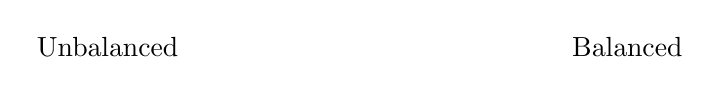
\begin{tikzpicture}
      \DSPECTRUM{4}{2}{1}
      \draw (-1.5,.5) node[align=right] {Unbalanced} ++(6.6,0) node[align=left] {Balanced};
    \end{tikzpicture}
  \caption{Visual representation of the equilibrium-state $(2:4)$. The size of the full x-axis is $M=4$ and the length of the bar is $I=2$. The left side of the spectrum is equivalent to the unbalanced equilibrium-state, and the right the balanced state.}\label{fig:eqstate}
\end{figure}
For example, a cluster with $M=4$ requires 4 growth iterations to reach an equilibrium in potential matching weight in all nodes in the cluster. The equilibrium-state thus gives us an indication of the how near balanced-bloom a cluster performs. 
\begin{lemma}
  Let $(I_t, M_t)$ denote the equilibrium-state of a cluster just before an union with another cluster that causes a parity inversion, and $(I_{t+1}, M_{t+1})$ the equilibrium-state after union, then 
  \begin{equation}\label{eq:eqpropto}
    I_t \propto M_{t+1}.
  \end{equation}
\end{lemma}
\begin{proof}
  In the context of the equilibrium-state, the delayed bloom of nodes in cluster growth is equivalent to increasing the value of $I$ in the equilibrium-state. As $I_t\to M_t$, the difference between the radii of the prioritized and delayed nodes increases, thus also increases the iterations $M_a$ needed after the union and parity inversion. 
\end{proof}
Subsequent parity inversions cause a gradual but certain increase in $M$ of the equilibrium-state, depending on $(I_t:M_t)$ during the parity inversion at the union, requiring a growing number of growth iterations $I_{t+1}$ to reach the equilibrium-state $(M:M)_{t+1}$. As the lattice size is increased, the total number of unions of a cluster with other clusters also increases, leading to a growing number of parity inversions. Thus increasing the lattice size has the consequence that more growth iterations $I$ are needed to reach equilibrium-state $(M:M)$. This is the trade-off in the effectiveness of this algorithm. On the one hand, it is preferred that $I\to M$ to maximally occupy the equilibrium-state that is a heuristic for minimum-weight, but on the other, $I$ is also proportional to the number of iterations needed to actually reach $(M:M)$ due to parity inversions. 

\begin{definition}
  Let the \emph{equilibrium factor} $f_{eq}\in [0,1]$ be a target factor to the node delay. 
\end{definition}
\begin{lemma}
  The delay equation where the delays have a factor $f_{eq}\in [0,1]$ minimizes the trade-off caused by parity inversion. 
  \begin{multline}
    s_\beta.d = s_\alpha.d + \Bigg \lceil f_{eq} \Bigg( 2\bigg(\ceil{\frac{s_\beta.r}{2}} - \floor{\frac{s_\alpha.r + s_\beta.r \bmod 2}{2}} - (-1)^{s_\beta.p}\abs{(s_\beta,s_\alpha)}\bigg)
    \Bigg) - \\
    (s_\beta.r - s_\alpha.r) \bmod 2 \Bigg \rceil \hspace{1em} | \hspace{1em} s_\beta \neq s_r. \tag{\ref{eq:delayequation}}
  \end{multline}
\end{lemma}
\begin{proof}
  For any $f_{eq} < 1$, a cluster will never actually reach the $(M:M)$ equilibrium-state, but only $(f_{eq}M:M)$. Consequently, after a parity inversion, the difference in node radii between prioritized and delayed nodes is decreased, such $I\to f_{eq}M$ can be reached in a lower amount of growth iterations. 
\end{proof}

The optimal value of $f_{eq}$ is dependent on the number of parity inversions, and consequently the lattice size, growth iteration, and the node-tree and cluster sizes $|\nset|, |\vset|$, with the goal of maximally occupying the equilibrium-state after the last parity inversion. We suspect that due to the fact that $M$ doubles after parity inversion, a constant factor of $f_{eq}=1/2$ should behave well on average. However, other values of $f_{eq}$ should be explored and optimizations dependent on these variables could be possible. 

\tikzstyle{edge}=[above,midway,font=\tiny]
\newcommand\DLINE[4]{
  \draw (#1, #2) ++ (-.3,-.9) node[inner sep=0] (lb) {} ++(#3,0) ++(.6,0) node[inner sep=0] (rb) {} ++(0,0.4) node[inner sep=0] (rt) {};;
  \path[fill=white!80!black, rounded corners=2pt] (lb) rectangle (rt);
  \ifnumequal{#4}{1}{\draw[thin] (lb) -- (rb);}{}
}
\begin{figure}[htbp]
\centering
    \begin{tikzpicture}[on grid, scale=1]
      \foreach \x in {0,3,6}{\DLINE{\x}{0}{2}{1}}
      \foreach \x in {0,2,3,5,6,8}{\draw (\x,0) node [even] (a\x) {1} ++(0,-.7) node (ad\x) {0};}
      \foreach[count=\i] \x in {1,4,7}{      \draw (\x,0) node [odd]  (a\x) {1} ++(0,-.7) node (ad\x) {2};
                                             \node at (\x,0.7) {$\nset_\i$};}
      \foreach \x in {0.5,3.5,6.5}{\DSPECTRA{2}{0}{\x}{-1.5}{0.3}{0.5}}
      \draw[l1] (a0) -- (a1) node[edge]{1} -- (a2) node[edge]{1} (a3) -- (a4) node[edge]{1} -- (a5) node[edge]{1} (a6) -- (a7) node[edge]{1} -- (a8) node[edge]{1};

      \begin{scope}[shift={(0,-3)}]
      \foreach \x in {0,3,6}{\DLINE{\x}{0}{2}{0}}
      \foreach \x in {0,2,3,5,6,8}{\draw (\x,0) node [even] (e\x) {2} ++(0,-.7) node {0};}
      \foreach \x in {1,4,7}{      \draw (\x,0) node [odd]  (e\x) {1} ++(0,-.7) node {1};}
      \foreach \x in {0.5,3.5,6.5}{\DSPECTRA{2}{1}{\x}{-1.5}{0.3}{0.5}}
      \draw[l1] (e0) -- (e1) node[edge]{1} -- (e2) node[edge]{1} (e3) -- (e4) node[edge]{1} -- (e5) node[edge]{1} (e6) -- (e7) node[edge]{1} -- (e8) node[edge]{1};
      \draw[l1, dashed] (e2) -- (e3) (e5) -- (e6);
      \end{scope}

      \begin{scope}[shift={(0,-6)}]
      \DLINE{0}{0}{8}{1}
      \foreach \x in {0,2,6,8}{\draw (\x,0) node [even] (b\x) {2} ++(0,-.7) node {0};}
      \foreach \x in {1,7}{    \draw (\x,0) node [odd]  (b\x) {1} ++(0,-.7) node {1};}
      \foreach \x in {3,5}{    \draw (\x,0) node [odd]  (b\x) {2} ++(0,-.7) node {4};}
                               \draw (4,0)  node [even] (b4)  {1} ++(0,-.7) node {1};
      \DSPECTRA{4}{0}{3}{-1.5}{0.3}{0.5}
      \draw[l1] (b0) -- (b1) node[edge]{1} -- (b2) node[edge]{1} -- (b3) node[edge]{2} -- (b4) node[edge]{1} -- (b5) node[edge]{1} -- (b6) node[edge]{2} -- (b7) node[edge]{1} -- (b8) node[edge]{1};
      \end{scope}

      \node[anchor=east, align=right] at (-1,0) {$n_i.s$};
      \node[anchor=east, align=right] at (-1,-0.75) {$n_i.d$};
      \node[anchor=east, align=right] at (-1,-1.5) {$(I:M)$};
      \path (-3,-3) node[even]{} -- +(.5,0) node[anchor=west] {$n.p$ even}; 
      \path (-3,-4) node[odd]{} -- +(.5,0) node[anchor=west] {$n.p$ odd}; 
      \draw[semithick, ->] (9,-.75) to [out=-60, in=60] ++(0,-2.5);
      \draw[semithick, ->] (9,-3.75) to [out=-60, in=60] ++(0,-2.5);
      \node at (10, -2) [align=right, text width = 3cm] {\underline{PDC}, \codefunc{Grow}};
      \node at (10, -5) [align=right, text width = 3cm] {\codefunc{Join}, \underline{PDC}};

%       \draw[l1, ->] (a8) ++(1,-.35) -- +(0,-2) node[midway, right, text width = 5cm, align=left] {Grow and calculate \\delay with eq. \eqref{eq:2ddelay}};
%       \draw[l1, ->] (c8) ++(1,-.35) -- +(0,-2) node[midway, right, text width = 5cm, align=left] {Grow and calculate \\delay with eq. \eqref{eq:delayequation},\\ $K_{bloom} = 0.5$};
    \end{tikzpicture}
    \caption{The delay values $n_i.d$ and the equilibrium-states $(I:M)$ for 3 odd clusters $\{\nset_1, \nset_2, \nset_3\}$ of 3 nodes that grow and join into a size-9 cluster. Initially (top), parity and delay calculations (PDC) are performed with delay equation \eqref{eq:2ddelay} on each odd cluster which have equilibrium-states $(0:2)$, with delay $2$ in the middle node. The clusters are grown (middle), where the middle node is delayed, such that it's delay value decreases to $1$, and the clusters have equilibrium-states $(1:2)$. The clusters join (bottom) to a single odd cluster, which is selected for growth. Hence PDC is performed again, and the equilibrium-state is $(0:4)$, thus requiring 4 growth iterations before equal potential matching weight is reached in all nodes.}\label{fig:kbloom}
\end{figure}

\begin{figure}[htbp]
  \centering
  \begin{tikzpicture}
      \foreach \x in {0,3,6}{\DLINE{\x}{0}{2}{1}}
      \foreach \x in {0,2,3,5,6,8}{\draw (\x,0) node [even] (c\x) {1} ++(0,-.7) node {0};}
      \foreach[count=\i] \x in {1,4,7}{      \draw (\x,0) node [odd]  (c\x) {1} ++(0,-.7) node (cd\x) {2};
                                             \node at (\x,0.7) {$\nset_\i$};}
      \foreach \x in {.75,3.75,6.75}{\DSPECTRA{1}{0}{\x}{-1.5}{0.3}{0.5}}
      \draw[l1] (c0) -- (c1) node[edge]{1} -- (c2) node[edge]{1} (c3) -- (c4) node[edge]{1} -- (c5) node[edge]{1} (c6) -- (c7) node[edge]{1} -- (c8) node[edge]{1};

      \begin{scope}[shift={(0,-3)}]
      \foreach \x in {0,3,6}{\DLINE{\x}{0}{2}{0}}
      \foreach \x in {0,2,3,5,6,8}{\draw (\x,0) node [even] (c\x) {2} ++(0,-.7) node {0};}
      \foreach \x in {1,4,7}{      \draw (\x,0) node [odd]  (c\x) {1} ++(0,-.7) node {0};}
      \foreach \x in {.75,3.75,6.75}{\DSPECTRA{1}{1}{\x}{-1.5}{0.3}{0.5}}
      \draw[l1] (c0) -- (c1) node[edge]{1} -- (c2) node[edge]{1} (c3) -- (c4) node[edge]{1} -- (c5) node[edge]{1} (c6) -- (c7) node[edge]{1} -- (c8) node[edge]{1};
      \draw[l1, dashed] (e2) -- (e3) (e5) -- (e6);
      \end{scope}

      \begin{scope}[shift={(0,-6)}]
      \DLINE{0}{0}{8}{1}
      \foreach \x in {0,2,6,8}{\draw (\x,0) node [even] (d\x) {2} ++(0,-.7) node {0};}
      \foreach \x in {1,7}{    \draw (\x,0) node [odd]  (d\x) {1} ++(0,-.7) node {0};}
      \foreach \x in {3,5}{    \draw (\x,0) node [odd]  (d\x) {2} ++(0,-.7) node {2};}
                               \draw (4,0)  node [even] (d4)  {1} ++(0,-.7) node {0};
      \draw[l1] (d0) -- (d1) node[edge]{1} -- (d2) node[edge]{1} -- (d3) node[edge]{2} -- (d4) node[edge]{1} -- (d5) node[edge]{1} -- (d6) node[edge]{2} -- (d7) node[edge]{1} -- (d8) node[edge]{1};
      \DSPECTRA{2}{0}{3.5}{-1.5}{0.3}{0.5}
      \end{scope}

      \node[anchor=east, align=right] at (-1,0) {$n_i.s$};
      \node[anchor=east, align=right] at (-1,-0.75) {$n_i.d$};
      \node[anchor=east, align=right] at (-1,-1.5) {$(I:M)$};
      \path (-3,-3) node[even]{} -- +(.5,0) node[anchor=west] {$n.p$ even}; 
      \path (-3,-4) node[odd]{} -- +(.5,0) node[anchor=west] {$n.p$ odd}; 
      \draw[semithick, ->] (9,-.75) to [out=-60, in=60] ++(0,-2.5);
      \draw[semithick, ->] (9,-3.75) to [out=-60, in=60] ++(0,-2.5);
      \node at (10, -2) [align=right, text width = 3cm] {\underline{PDC}, \codefunc{Grow}};
      \node at (10, -5) [align=right, text width = 3cm] {\codefunc{Join}, \underline{PDC}};

  \end{tikzpicture}
  \caption{The same clusters, growths and joins as in Figure \ref{fig:kbloom}, but now with delay equation \eqref{eq:delayequation} for $f_{eq} = 1/2$. With the equilibrium factor, $(f_{eq}M:M)$ can be reached in fewer growth iterations; e.g. after 1 round (middle), $(1:1)$ is reached. Also after join to a single cluster (bottom), fewer iterations are needed (2 compared to 4 in Figure \ref{fig:kbloom}).}\label{fig:kbloom2}
\end{figure}
 
\subsection{Parity and delay calculations}\label{sec:pdccalc}

With equation \eqref{eq:nodeparity} and \eqref{eq:delayequation}, we now finally have the tools to formulate the algorithms to calculate the node parities and delays. For a node set with root $n_r$, we can calculate the parities by calling the \emph{head recursive} function \codefunc{CalcParity} on $n_r$ in algorithm \ref{al:calcparity}, where we do a reverse DFS of the node-tree. The node delays are calculated by calling the \emph{tail recursive} function \codefunc{CalcDelay} in algorithm \ref{al:calcdelay}, where we perform a second DFS of the node-tree. These Parity and Delay Calculation will from this point be referred to as the PDC. A schematic of the directions of these calcultions in an example node-tree is included in Figure \ref{fig:2dfs}.

\begin{algorithm}[htbp]
  \SetKwData{node}{node}
  \SetKwData{cluster}{cluster}
  \SetKwData{child}{child}
  \SetKwData{parity}{parity}
  \SetKwData{pary}{p}
  \SetKwFunction{cp}{CalcParity}
  \SetKwFunction{summation}{Sum}

  \KwData{\node}
  \KwResult{Defined parities for all children of \node}

  \BlankLine

  \parity $=$ \summation{$[1 - $ \cp{\child} $\forall$ \child of \node $]$} $\%2$\;
  \uIf{\node $\equiv \sigma$}{
      \node.\pary $=$ \parity}
  \uElseIf{\node $\equiv j$}{
      \node.\pary $= 1-$ \parity}
  \KwRet{\node.\pary}
  \caption{\codefunc{CalcParity}}\label{al:calcparity}
\end{algorithm}


\begin{algorithm}[htbp]
  \SetKwData{node}{node}
  \SetKwData{cluster}{cluster}
  \SetKwData{child}{child}
  \SetKwData{delay}{d}
  \SetKwFunction{cdelay}{CalcDelay}

  \KwData{\node, \cluster}
  \KwResult{Defined parities for all children of \node}

  \BlankLine

  \If{\node has an ancestor}{
    calculate \node.\delay with equation \eqref{eq:delayequation}\;
    \If{\node.\delay $<$ \cluster.\delay}{
      \cluster.\delay $=$ \node.\delay
      }
    }
  \For{\child of \node}{
    \cdelay{\child, \cluster}
  }
  \caption{\codefunc{CalcDelay}}\label{al:calcdelay}
  \end{algorithm}


\begin{figure}
  \centering
  \begin{tikzpicture}[x=1.5cm,y=1.5cm]
    \node[node1,even] (a) at (1, 3) {$n_r$};
    \node[node1,odd]  (b) at (1, 2) {};
    \node[node1,odd]  (c) at (1, 1) {};
    \node[node1,even] (d) at (1, 0) {};
    \node[node1,even] (e) at (0, 1) {};
    \node[node1,even] (f) at (0, 0) {};
    \node[node1,odd]  (g) at (2, 2) {};
    \node[node1,even] (h) at (2, 1) {};
    \node[node1,even] (i) at (2, 0) {};
    \draw[l1] (a) -- (b) -- (c) -- (d);
    \draw[l1] (b) -- (e);
    \draw[l1] (c) -- (f);
    \draw[l1] (c) -- (i);
    \draw[l1] (a) -- (g) -- (h);

    \draw[l1, ->, dashed, color=mblue] (0, 1.3) -- +(45:0.85) arc (-45:0:.5) -- +(90:.6);
    \draw[l1, ->, dashed, color=mblue] (0, 0.3) -- +(45:0.85) arc (-45:0:.5) -- +(90:.2);
    \draw[l1, ->, dashed, color=mblue] (0.75,0.2) -- +(90:.3);
    \draw[l1, ->, dashed, color=mblue] (1.5,0.2) -- +(135:.4);
    \draw[l1, ->, dashed, color=mblue] (1.75,1.2) -- +(90:0.5) arc (0:45:.5) -- +(135:0.4);
    \draw[l1, ->, color=mred] (1.4, 3) -- +(-45:1.1) arc (45:0:0.5) -- +(-90:0.7);
    \draw[l1, ->, color=mred] (1.3, 2.1) -- +(-90:0.9) arc (180:225:.5) -- +(-45:0.7);
    \draw[l1, ->, color=mred] (0.6, 1.3) -- +(225:.3);
    \draw[l1, ->, color=mred] (0.6, 0.3) -- +(225:.3);
    \draw[l1, ->, color=mred] (1.3, 0.3) -- +(-90:.2);
    \node[text=mblue] at (0,2.2) {Parity};
    \node[text=mred] at (2.6,2.8) {Delay};
    \node at (0,3) {$\mathcal{N}$};
  \end{tikzpicture}
  \caption{The parity and delay calculation (PDC) performed on a the root node $n_r$, which is equivalent to two depth-first searches on $\mathcal{N}$ to compute node parities (head recursively) and delays (tail recursively).}\label{fig:2dfs}
\end{figure}


\section{Growing a cluster}\label{sec:growingcluster}
With the knowledge of previous section, we now have the equations and algorithms available to describe the steps to grow a cluster in the context of Balanced Bloom. In the node data structure, the growth of a cluster is equivalent to a DFS of the node set. The boundary list for each cluster is not stored at $C$, but separately stored at each of the nodes $n_i$ in $\m{N}$. We traverse all $n_i \in \m{N}$ from the root $n_r$ and apply $\codefunc{Bloom}(n_i)$, which increases the support of all boundary edges in $n_i.m{L}$ by 1.

Recall from theorem \ref{def:balancedbloom} that with Balanced Bloom, we need to conditionally bloom the nodes with minimal PMW, or zero PNW. Also, from lemma \ref{lem:calconce}, the delays are not recalculated after each growth iteration (in the absence of unions) but stored in memory at the nodes, and the PNW is updated via $n.w$ (equation \eqref{eq:pnw}), the number of growths a node has waited. Thus, we can define a function $\codefunc{Grow}(n_i)$ where $\codefunc{Bloom}(n_i)$ is only applied if $PNW(n_i) = n_i.d - C.d - n_i.w = 0$ is satisfied. If not, node $n_i$ is skipped, the wait is increased $n_i.w = n_i.w +1$ and \codefunc{Bloom} is recursively applied on its children.

New vertices $v_{new}$ grown from node $n_i$ are added to $\m{V}$, while storing the seed node at each new vertex $v_{new}.n = n_i$. New boundary edges are appended to the boundary list $n_i.\m{L}$ stored each seed node $n_i$. The number of nodes in $\m{N}$ and the shape of the flower bush tree therefore does not change while no merge between clusters has happened.

\begin{theorem}\label{the:grownode}
  A cluster $C$ is grown by calling $\codefunc{Grow}(n)$ on the root node $n_r$, which first checks for the wait of the current node $ n.d - C.d - n.w = 0$ to grow its boundary edges with $\codefunc{Bloom}(n)$, and then recursively applies \codefunc{Grow} to its children.
\end{theorem}


\begin{algorithm}[htbp]

  \SetKwData{node}{node}
  \SetKwData{child}{child}
  \SetKwData{cluster}{cluster}
  \SetKwData{delay}{d}\SetKwData{waited}{w}
  \SetKwData{edge}{edge}\SetKwData{support}{support}
  \SetKwFunction{grow}{Grow}
  \SetKwFunction{bloom}{Bloom}

  \KwData{\node}
  \KwResult{A node that has either grown or waited one iteration.}

  \BlankLine

  \eIf{\node.\delay $-$ \cluster.\delay $-$ \node.\waited $=0$}{
    \bloom{\node}, add all edges \edge.\support $= 2$ to $\m{F}$
  }{
    \node.\waited $+=1$
  }
  \For{\child of \node}{
    \grow{\child}
  }
  \caption{\codefunc{Grow}}\label{al:bbgrow}
\end{algorithm}


\section{Joining node sets}\label{sec:jointnodesets}
With the extension of the node set data structure, during a union of clusters $C_\alpha$ and $C_\beta$, we have to additionally combine the node sets $\m{N}_{\alpha}$ and $\m{N}_\beta$ that requires its own set of rules that we will explain in this section. Let us first make a clear distinction between the various routines. On the vertex set $\m{V}$ we apply $\codefunc{Union}(v^\alpha, v^\beta)$, on the two vertices spanning the edge connecting two clusters. On node set $\m{N}$, we introduce here $\codefunc{Join}(n^\alpha, n^\beta)$, which is called on the two nodes $n^\alpha, n^\beta$ that seed vertices $v^\alpha, v^\beta$, respectively. During a merge of two clusters, these routines are both applied on their respective sets. From this point, when either one of the expressions "merge clusters $C^\alpha$ and $C^\beta$", "the union of vertex sets $\m{V}_\alpha$ and $\m{V}_\beta$" or the "join of node sets $\m{N}_{\alpha}$ and $\m{N}_\beta$" is mentioned, it is always implied that both routines are executed.

Within the vertex set $\m{V}$, we apply \emph{path compression} and \emph{weighted union} to minimize the depth of the tree and therefore minimizing the calls to the \codefunc{Find} function. Similarly, in the node set $\m{N}$, we would also like to apply a set of rules to minimize the calls to \codefunc{CalcParity} and \codefunc{CalcDelay}, which are the parity and delay calculation(s) (PDC). As the structure of the tree is crucial in computing the parity of the nodes and relative delays between the nodes, these rules will be quite different than in vertex set $\m{V}$ that changes the ancestry dynamically by path compression. Join rules will be dependent on the parities of the joining node sets $\m{N}.p$, which is the number of syndrome-nodes in the set modulo 2. The parity of a node set $\m{N}.p$ is equivalent to the parity of a cluster $C.p$, which also refer to the number of syndromes in the cluster.
\begin{lemma}
  The parity of node set $\m{N}.p$ is the number of syndrome-nodes $a_i \in \m{N}$ modulo 2. The parity of node set $\m{N}.p$ is analogous to cluster parity $C.p$.
\end{lemma}

Only odd clusters with odd parity node sets are grown in the UF-decoder. It may thus be tempting to conclude that a join must include at least one odd node set. This is however not true as within the same growth iteration, there may be many joins, where some odd cluster $\nset_1^o$ first joins with odd cluster $\nset_2^o$, but also joins with even cluster $\nset_3^e$. The second join is effectively between even clusters. Hence there are 3 types of joins: 1) odd-odd, 2) even-odd and 3) even-even, where even-odd is equivalent to odd-even. These joins can be put into 2 \emph{classes}, dependent on the parity of the resulting cluster. Both odd-odd and even-even joins to an even cluster and thus belongs to the even class join (E-join), whereas even-odd (and odd-even) joins to an odd cluster in the odd class join (O-join).


\subsection{E-joins}

For E-joins, the joined even cluster $\nset^e$ will not be selected for growth by the UF-decoder. One could naively conclude that no PDC will be performed and no PDC minimization can be made. This is of course not true as it is entirely possible that another cluster grows, and merges with the cluster of $\m{N}^{e}$ in a O-join. In that case, we might think about "reusing" some of the node parities and delays that were already calculated in the subsets of $\m{N}^e$, such that $\m{N}^{e}$ doesn't have to be traversed entirely for its parities and delays. In this case, a \emph{partial PDC} is performed over the undefined part.

To reuse prior calculated parities and delays, we need to traverse $\nset^e$ to find which sections are still valid, and which sections are not. This is no trivial task and often requires us to traverse the entire set $\nset^e$, especially when the clusters in the E-join are the results of joins within the same growth iteration.  Checking the validity to reuse prior parities and delays then acquires the same complexity as redoing the PDC over the subset $\nset^e$. Hence the node parities and delays in the joined set after an E-join are \emph{undefined}.

\begin{lemma}\label{lem:nodecalc_even}
  Node parities and delays become undefined if multiple node sets joins into a new set $\m{N}$ with even parity.
\end{lemma}

\subsection{O-joins}

Consider now an O-join between an even node set $\m{N}^e$ and an odd node set $\m{N}^o$ in nodes $n^e, n^o$ respectively, and assume that this join is due to the growth of odd cluster $\m{N}^o$ onto an "idle" $\m{N}^e$. The join of these two sets produces a new odd node set $\m{N}_{new}^o$ with subsets $'\nset^e$ and $'\nset^o$, referring to the original node sets. We are provided with two choices, A) make $n^e$ child of $n^o$, or B) make $n^o$ child of $n^e$. The ancestry in the parent node set stays unchanged, but the ancestry in the child subset is changed by setting the joining node in the child set $n^c$ as the sub-root of the child subset $'\m{N}^c$. This is allowed per lemma \ref{lem:anynoderoot}, but removes any calculated parities or delays per lemma \ref{lem:anynoderoot} and \ref{lem:nodecalc_ancestrypath}.

For option A, an even number of nodes of $'\m{N}^e$ is attached to $n^o$, and the ancestry in $'\m{N}^o$ hasn't changed. The parities and delays in $'\m{N}^o$ stay valid and can be reused. From $n^e$, which is now the sub-root of  $'\m{N}^e$, a partial PDC is applied, where the relative delay of $n^e$ is calculated with respect to its parent $n^o$ (Figure \ref{fig:joinrules}A). This is efficient as the parities and delays in $'\m{N}^e$ are already undefined per lemma \ref{lem:nodecalc_even}. For option B, we need to redo the PDC in both $'\m{N}^o$ and $'\m{N}^e$ (Figure \ref{fig:joinrules}B), as $'\m{N}^o$ has a changed ancestry and  $'\m{N}^e$ is even. The PDC is thus minimized if option A is always chosen. \\

% If the subset $'\m{N}^e$ consists of only two odd node sub-subsets $''\m{N}^o_0, ''\m{N}^o_1$, where $n_0, n_1$ are the joining nodes, the ancestry in $''\m{N}^o_0$ is preserved and $n_1$ is the sub-root of $''\m{N}^o_1$. We see that the parities in all ancestors of $n_0$ are flipped. Let's consider the cases and find whether we can minimize the parity and delay calculation in $'\m{N}^{e}$.
%
% For case a), an even number of nodes of $'\m{N}^e$ is attached to $n^o$, and the ancestry in $'\m{N}^o$ hasn't changed. This means that the parities in $'\m{N}^o$ do not change per lemma \ref{lem:anynoderoot}, and the delays in $'\m{N}^o$ are still valid as per lemma \ref{lem:nodecalc_ancestrypath}. In $'\m{N}^e$, as the ancestry path has changed, we are certain to traverse $'\m{N}^e$ from the sub-root $n^e$ to calculate the delays in this subset which is in the order of $S_{'\m{N}^e}$.
%
% In case b), as an odd number of nodes of $'\m{N}^o$ is attached to $n^e$, it means that parities of all ancestor of $n^e$ are flipped. As the ancestry in $'\m{N}^{o}$ has changed, we are certain to traverse $'\m{N}^o$ from the sub-root $n^o$ to calculate the delays which is in the order of $S_{'\m{N}^o}$. The node parity changes in $'\m{N}^e$ will be dependent on the location of $n^e$ in the ancestry compared to $n^1$ and $n^2$, and all children nodes of these parity changes will have to recalculate their delays. Let's call the number of nodes needs to calculate parity and delays in $'\m{N}^e$ a value $S_e \leq S_{'\m{N}^e}$, leaving the total number of operations in the order of $S_e + S_{'\m{N}^o}$.
%
% For $'\m{N}^e$ consisting of two subsets, keeping track of the parity changes between $n^e$, $n^0$ and $n^1$ is still an easy task, and we might gain in minimization in operations in case b) compared to case a) for some value $S_e$ such that $S_e + S_{'\m{N}^o} < S_{'\m{N}^e}$. But as the number of subsets in $'\m{N}^e$ increases, the task of finding the ancestry paths of parity changes becomes analogous to traversing $'\m{N}^e$ entirely $S_e \rightarrow S_{'\m{N}^e}$. To simplify, we always choose case a.
The rules are thus very simple for the function $\codefunc{Join}(n^\alpha, n^\beta)$. For O-joins between an even and an odd node set $\nset^e, \nset^o$ in the nodes $n^e, n^o$, always make the even node set a child of the even node set, where $n^e$ is now the sub-root of the subset $'\nset^e$. For E-joins between two even or two odd node sets, the parent and child sets can be picked at random. Finally, we note the concept of a $partial$ PDC is rather redundant, as a PDC is always applied partially on the undefined part of a set for any set with $S_\nset>1$.

\begin{theorem}\label{the:nodejoint}
  The union of node sets $\m{N}^\alpha, \m{N}^\beta$ on nodes $n^\alpha, n^\beta$ respectively is performed with $\codefunc{Join}(n^\alpha, n^\beta)$. If the join is between an even and an odd node set $\nset^e, \nset^o$ in the nodes $n^e, n^o$, $\codefunc{Join}(n^e, n^o)$ makes the node of the even set $n^e$ a child of the node of the odd set $n^o$. If the join is between two even or two odd node sets, the choice is arbitrary.
\end{theorem}

\begin{figure}
\centering
\begin{tikzpicture}[on grid]
  \node (o1) [even] at (1.5, 1) {$n_1$};
  \node (o2) [even] at (1, 0) {$n_2$};
  \node (o3) [even] at (2, 0) {$n_3$};
  \node (e4) [undef] at (3.5,1) {$n_4$};
  \node (e5) [undef] at (3.5,0) {$n_5$};
  \draw[l1] (o2) -- (o1) -- (o3) (e4) -- (e5);
  \draw[l1, dashed] (o3) -- (e5) node[midway,below] (a) {};
  \draw[l1, <-] (a) -- ++(0,-.5) node[below] {$\codefunc{Join}(n_3, n_5)$};

  \begin{scope}[shift={(5,1)}]
  \node (o1) [even] at (1.5, 1) {$n_1$};
  \node (o2) [even] at (1, 0) {$n_2$};
  \node (o3) [even] at (2, 0) {$n_3$};
  \node (e4) [undef] at (2,-2) {$n_4$};
  \node (e5) [undef] at (2,-1) {$n_5$};
  \draw[l1] (o2) -- (o1) -- (o3) -- (e5) -- (e4);
  \draw[l1, ->, dashed, color=mblue] (e4) ++(-.7,0) -- + (0,1);
  \draw[l1, ->, color=mred] (o3) ++(.7,-.5) -- +(0,-1.5);
  \end{scope}

  \begin{scope}[shift={(10,1.5)}]
  \node (o1) [even] at (1, -2) {$n_1$};
  \node (o2) [even] at (1, -3) {$n_2$};
  \node (o3) [even] at (1, -1) {$n_3$};
  \node (e4) [undef] at (1,1) {$n_4$};
  \node (e5) [undef] at (1,0) {$n_5$};
  \draw[l1] (o2) -- (o1) -- (o3) -- (e5) -- (e4);
  \draw[l1, ->, dashed, color=mblue] (o3) ++(-.7,.5) -- +(0,1.5);
  \draw[l1, ->, dashed, color=mblue] (o2) ++(-.7,0) -- +(0,2);
  \draw[l1, ->, color=mred] (e4) ++(.7,0) -- +(0,-1);
  \draw[l1, ->, color=mred](e5) ++(.7,-.5) -- + (0,-2.5);
  \end{scope}

  \node at (5,2) {A)};
  \node at (9.5,2) {B)};
\end{tikzpicture}
\caption{An odd cluster $\nset^e=\{n_1, n_2, n_3\}$ with root $n^e_r = n_1$ joins with an odd cluster $\nset^o=\{n_4, n_5\}$ with root $n^o_r=n^4$ on nodes $n_3, n_5$, respectively, to a new set $\nset$ with subsets $'\nset^e$ and $'\nset^o$. Here we use dotted outlines on the nodes of $'\nset^e$ to indicate that their parities and delays are undefined. If we choose to A), make $n_5$ a child of $n_3$, the parities and delays in $'\nset^o$ can be reused, and we only have to redo PDC over $'\nset^e$. If we choose to B), make $n_3$ a child of $n_5$, PDC's have to be redone over both $'\nset^o$, as it has a new sub-root $n_3$, as well as $'\nset^e$ as its parties and delays were undefined.}\label{fig:joinrules}
\end{figure}

\subsection{Prevention of redundant PDC's}\label{sec:multiplejoint}
The final rule for joins between clusters introduces a data structure to store undefined parts of a cluster, such that multiple PDC's over a subset is prevented. If there are many O-joins (and E-joins) within the same growth iteration $i$, that at the end of $i$ results to one single cluster $\nset$, every O-join will require the PDC over the even subset. There may be subsets where multiple PDC's are performed before the final cluster $\nset$ is constructed. If the PDC is done directly after an O-join, the calculated values may thus be redundant.

Consider an example with 5 odd clusters $\nset_1, ...,  \nset_5$ (Figure \ref{fig:redundantpdc}). The join of $\nset_1$ and $\nset_2$ to $\nset_{12}$ is an E-join and requires no PDC. The join of $\nset_{12}$ and $\nset_3$ is an O-join, and we apply PDC in $\nset_{12}$. The join of $\nset_{123}$ and $\nset_4$ is an E-join and the join of $\nset_{1234}$ and $\nset_5$ is an O-join, with PDC executed in $\nset_{1234}$. The earlier computation in $\nset_{12}$ was therefore unnecessary and possibly invalid.

\tikzstyle{enset}=[node1, thick, double, font=\footnotesize]
\tikzstyle{onset}=[node1, thick, densely dashed, double, font=\footnotesize]

\begin{figure}
\centering
\begin{tikzpicture}
  \node (n1) [onset] at (0,0) {$\nset_1$};
  \node (n2) [onset] at (0,-1) {$\nset_2$};
  \draw[l1, dashed] (n1) -- (n2);

  \begin{scope}[shift={(3,-.5)}]
  \node (n3) [onset] at (0,1) {$\nset_3$};
  \node (n1) [onset] at (0,0) {$\nset_1$};
  \node (n2) [onset] at (0,-1) {$\nset_2$};
  \draw[l1, dashed] (n3) -- (n1); \draw[l1] (n1) -- (n2);
  \draw[l1, ->, dashed, color=mblue] (n2) ++(-.7,0) -- +(0,1);
  \draw[l1, ->, color=mred] (n1) ++(.7,0) -- +(0,-1);
  \end{scope}

  \begin{scope}[shift={(6.5,-.5)}]
  \node (n3) [onset] at (0,1) {$\nset_3$};
  \node (n1) [onset] at (0,0) {$\nset_1$};
  \node (n2) [onset] at (-.5,-1) {$\nset_2$};
  \node (n4) [onset] at (.5,-1) {$\nset_4$};
  \draw[l1, dashed] (n1) -- (n4); \draw[l1] (n3) -- (n1) -- (n2);
  \end{scope}

  \begin{scope}[shift={(10,-1)}]
  \node (n5) [onset] at (0,2) {$\nset_5$};
  \node (n3) [onset] at (0,1) {$\nset_3$};
  \node (n1) [onset] at (0,0) {$\nset_1$};
  \node (n2) [onset] at (-.5,-1) {$\nset_2$};
  \node (n4) [onset] at (.5,-1) {$\nset_4$};
  \draw[l1, dashed] (n3) -- (n5); \draw[l1] (n3) -- (n1) -- (n2) (n1) -- (n4);
  \draw[l1, ->, dashed, color=mblue] (n2) ++(-.7,0) -- +(0,2);
  \draw[l1, ->, color=mred] (n3) ++(1.2,0) -- +(0,-2);
  \end{scope}

  \node at (-1, 1) {a)};
  \node at (2, 1) {b)};
  \node at (5.5, 1) {c)};
  \node at (9, 1) {d)};
\end{tikzpicture}
\caption{If the PDC is directly performed on the even subset in an O-join, there may be redundant PDC's in a series of O-joins and E-joins within the same growth iteration. Here we picture a series of join events between odd node sets (double lined circles, dashed for odd parity), where the O-join in b) initiates a redundant PDC.}\label{fig:redundantpdc}
\end{figure}

Note that some odd node set $\nset^o$ must always consist of some odd part $'\nset^o$ and an even part $'\nset^e$. The even part $'\nset^e$ may be subdivided into a number of odd and even sub-subsets $''\nset$, as long as the sum of their parities is even. Let us call the \emph{final O-join} between $'\nset^e$ and $'\nset^o$ in a series of joins between clusters within the same growth iteration a \emph{FO-join}, and all others O-joins that play a role in constructing $'\nset^e$ \emph{intermediate O-joins} or \emph{IO-joins}. The PDC needs only to be executed on the even subset in the FO-join $'\nset^e$.
\begin{lemma}\label{lem:oddisevenodd}
  An odd node set $\nset$ that is the result of some joins must consist of an odd subset $'\nset^o$ and an even subset $'\nset^e$, where the even subset $'\nset^e$ may consist of smaller sub-subsets $''\nset$.
\end{lemma}
To circumvent the PDC multiplicity, the calculation is suspended as much as possible. The parities and delays are required for the growth of a cluster. Thus the PDC is to be executed just before a cluster is grown, not when some O-join has occurred.
\begin{lemma}\label{lem:delaywhengrown}
  Parity and delay calculations are only performed on the undefined part of a node set when a cluster is grown, not directly after a join.
\end{lemma}

The only task now is to store where the even subset $'\nset^e$ of the FO-join starts in the ancestry of subset $\nset^o$, as the sub-root of $'\nset^e$ is the starting point of the DFS's of the PDC. For each join between odd node set $'\m{N}^o$ and even node set $'\m{N}^e$ on nodes $'n^o, 'n^e$, we additionally store the sub-root $'n^e_r$ of subset $'\m{N}^e$ at the root node of the resulting set $\m{N}^{o}$ as $n^{o}_r.u$, the \emph{undefined} sub-root. If $\m{N}^{o}$ is selected for growth, we apply $\codefunc{CalcParity}(n^{o}_r.u)$ and $\codefunc{CalcDelay}(n^{o}_r.u)$ calculate parities and delays in undefined parts of the set, if it exists. The recursiveness of these function will make sure that the PDC are performed on all children nodes of (and including) $n^{o}_r.u$. We then call $\codefunc{Bloom}(n_r)$ per theorem \ref{the:grownode}.

This data structure dynamically saves the root of the undefined part of a cluster to the root node. For any IO-join, we don't know yet whether another O-join will occur, thus each IO-join to cluster $''\nset^o$ is treated as a FO-join. For a IO-join, we thus also store the undefined sub-root $u_1$ at the root $r_1=''n_r^o$. If $''\nset^o$ joins with other clusters in subsequent E-join to cluster $'\nset^e$ and lastly the "real final" FO-join with $'\nset^o$ to $\nset^o$, we again store the undefined sub-root $u_2='n_r^e$ at the new root of $r_2='n_r^o$. Due to theorem \ref{the:nodejoint}, it is certain that $u_2$ is an ancestor of $u_1$, and the PDC will traverse over all undefined regions of the set.

\begin{theorem}\label{the:delayonce}
  Undefined region of an odd cluster $\nset^o$ is defined as the sub-root $u$ for which all children nodes including $u$ have undefined parities and delays, and is stored at root node $n^o_r$. PDC is performed for $n^o_r.u$ and its children before cluster $\nset^o$ is grown.
\end{theorem}

\section{Pseudo-code}
Now we have the full description of the \emph{Balanced Bloom} alteration of the UF decoder, which we dub the \emph{Union-Find Balanced Bloom} (UFBB) decoder. We present its pseudo-code in algorithm \ref{al:ufbb}. The recursive \codefunc{Grow} function of algorithm \ref{al:bbgrow} has been added fully to the pseudo-code in lines 7-12, as it is a crucial part of the decoder. Note that the structure of the code is mostly identical to the BCS UF decoder, where we sort the clusters growth in buckets, and apply the merge, in this case the combination of \codefunc{Union} and \codefunc{Join}, after each bucket iteration.

\begin{algorithm}[htbp]
  \SetKwData{bucket}{bucket}\SetKwData{buckets}{buckets}
  \SetKwData{edge}{edge}\SetKwData{support}{support}
  \SetKwData{node}{node}
  \SetKwData{cluster}{cluster}
  \SetKwData{child}{child}
  \SetKwData{delay}{d}\SetKwData{waited}{w}
  \SetKwFunction{calcdelay}{CalcDelay}
  \SetKwFunction{calcparity}{CalcParity}
  \SetKwFunction{place}{Place}
  \SetKwFunction{bloom}{Bloom}
  \SetKwFunction{join}{Join}
  \SetKwFunction{union}{Union}

  \KwData{\buckets}
  \KwResult{Set of even clusters grown according to Balanced Bloom}

  \BlankLine

  \For{\bucket in \buckets}{

    \For{\cluster in \bucket}{
      check if \cluster belongs is current \bucket \;
      \For{\node in \cluster.$\m{C}$}{
        \calcparity{\node}\;
        \calcdelay{\node, \cluster}
      }
      \eIf{\node.\waited $=$ \node.\delay $-$ \cluster.\delay}{
        \bloom{\node}, add all edges \edge.\support $= 2$ to $\m{F}$
      }{
        \node.\waited $+=1$
      }
      \For{\child of \node}{
        repeat lines 7-12 on \child
      }
    }
    \For{\edge in $\m{F}$}{
      \union{$v_1, v_2$} for \edge $= (v_1, v_2)$ \;
      \join{$n_1, n_2$} for $v_1, v_2$ seeded in nodes $n_1, n_2$
    }
    \place{\cluster} $\forall$ odd clusters
  }
  \caption{Union-Find Balanced Bloom decoder}\label{algo:ufbb}
\end{algorithm}


\section{Complexity of Balanced Bloom}\label{sec:ufbbcomplexity}

The contribution to the time complexity of the UF-EG decoder compared to the UF decoder can be divided into two parts. First is the contribution by \codefunc{CalcParity} and \codefunc{CalcDelay}, the parity and delay calculations (PDC), which is called \emph{PDC complexity}. The second contribution will be caused by \codefunc{Grow} of algorithm \ref{al:bbgrow}, as now we have to additionally traverse the node set tree's of each cluster to access its boundary edges and grow them with \codefunc{Bloom} as compared to a single boundary list per cluster. We call this second contribution the \emph{bloom complexity}.

\subsection{PDC complexity}
As per lemma \ref{lem:nodecalc_ancestrypath} and \ref{lem:nodecalc_even}, the total cost of the PDC is increased when the ancestries within subtrees change due to join operations, and node parities and delays have to be recalculated by traversal of the subtree. Per theorem \ref{the:nodejoint} and \ref{the:delayonce}, these calculations can be limited to the even subtrees in FO-joins. The size of the even subtrees in FO-joins, multiplied by the number of join operations thus estimates the count of these calculations. We will take a top-down approach to find these estimates, where we retrace the ancestor node sets in their join operations in what we call the \emph{fragmentation} of $\nset$.

\subsubsection{Fragmentation of a node set}

\begin{figure}
  \centering
  \begin{tikzpicture}[node distance=1cm, on grid]

    \node (a) at (0,0) {};
    \node (b) [right = 4cm of a] {};
    \node (c) [right = 5cm of b] {};

    \node (b1l) [below left = 1cm and 2cm of a] {};
    \node (b1r) [above right = 3.5cm and 2cm of b] {};
    \path[fill=black!10!white, rounded corners=0.5cm] (b1l) rectangle (b1r);
    \node (b1t) at ($(a)!0.5!(b)$) {}; \node [above=3cm of b1t] {generation $k$};
    \node (b2l) [below left = 1cm and 2cm of c] {};
    \node (b2r) [above right = 3.5cm and 2cm of c] {};
    \path[fill=black!10!white, rounded corners=0.5cm] (b2l) rectangle (b2r);
    \node [above=3cm of c] {generation $k-1$};

    \foreach \i in {0,1,2}{
        \node (a\i) [above = \i cm of a] {\footnotesize $\pre{k}\nset^o_\i$};
        \draw[densely dashed, thick, double] (a\i) circle[radius=.4cm];
    }

    \foreach \i in {0,1,2}{
        \node (b\i) [above = \i cm of b] {};
    }
    \node at (b2) {\footnotesize $\pre{k}\nset^o_0$};
    \node at ($(b0)!0.5!(b1)$) {\footnotesize $\pre{k}\nset^e$};
    \draw[densely dashed, thick, double] (b2) circle[radius=0.4cm];
    \draw[l1,opacity=0.3,dotted] (b1) circle[radius=.4cm];
    \draw[l1,opacity=0.3,dotted] (b0) circle[radius=.4cm];
    \node[right = 0.5cm of b] (bc) {};
    \draw[thick, double] (bc) -- +(0, 1) arc (0:180:0.5) -- +(0, -1) arc (180:360:0.5) -- cycle;

    \foreach \i in {0,1,2}{
      \node (c\i) [above =\i cm of c] {};
      \draw[l1,opacity=0.3,dotted] (c\i) circle[radius=.4cm];
    }
    \node[right = 0.5cm of c] (cc1) {}; \node[right = 0.6cm of c] (cc2) {};
    \draw[l1, opacity=0.3, dotted] (cc1) -- +(0, 1) arc (0:180:0.5) -- +(0, -1) arc (180:360:0.5) -- cycle;
    \draw[densely dashed, thick, double] (cc2) -- +(0, 2) arc (0:180:0.6) -- +(0, -2) arc (180:360:0.6) -- cycle;
    \node at (c1) {\footnotesize $\pre{k-1}\nset^o$};

    \node (f1a) [below left = 0.4cm and 0.4cm of c] {}; \node (f1b) [below right = 0.4cm and 0.4cm of b] {};
    \node (f2a) [below left = 0.4cm and 0.4cm of b] {}; \node (f2b) [below right = 0.4cm and 0.4cm of a] {};
    \node (fa) [below = 0.6cm of c] {}; \node (fb) [below = 0.6cm of a] {};
    \draw[l1, ->, dashed] (f1a) .. controls +(225:0.5cm) and +(315:0.5cm) .. (f1b);
    \draw[l1, ->, dashed] (f2a) .. controls +(225:0.5cm) and +(315:0.5cm) .. (f2b);
    \draw[l1, ->, dashed] (fa)  .. controls +(210:1cm) and +(330:1cm) .. (fb);

    \node (ca) at ($(c)!0.5!(a)$) {}; \node [below = 1.5cm of ca] {$f$};
    \node (cb) at ($(c)!0.5!(b)$) {}; \node [below = 0.4cm of cb] {$f_e$};
    \node [below = 0.4cm of b1t] {$f_o$};

    \node (u1lt) at ($(a0)!0.5!(a1)$) {}; \node(u1l) [right=1cm of u1lt] {};
    \node (u1rt) at ($(b0)!0.5!(b1)$) {}; \node(u1r) [left=1cm of u1rt] {};
    \node (u2lt) at ($(b1)!0.5!(b2)$) {}; \node(u2l) [right=1cm of u2lt] {};
    \node (u2rt) at ($(c1)!0.5!(c2)$) {}; \node(u2r) [left=1cm of u2rt] {};
    \draw[l1, ->] (u1l) -- (u1r) node[midway,above] {join};
    \draw[l1, ->] (u2l) -- (u2r) node[midway,above] {join};

  \end{tikzpicture}
  \caption{In the fragmentation of cluster $\pre{k+1}\nset^o$ that belongs to ancestral generation $k-1$, we find the clusters $\pre{k}\nset_j$ of which the joins constructed cluster $\pre{k+1}\nset^o$. Any odd cluster can be fragmented into an odd (double dashed) and even (double continuous) cluster.}\label{fig:generation}
\end{figure}

For each odd node set $\nset^o$ that is grown, it may have constructed by many joins of smaller ancestral node sets in some previous growth iteration. Before $\nset^o$ is grown, PDC is performed on the even subset $'\nset^e$ of the FO-join of its ancestral node sets, where its size is proportional to the \emph{PDC count} $N_{PDC}$, the number of calculations performed during PDC. Subset $'\nset^e$ may itself be the result of many IO-joins and E-joins in some previous growth iteration $i$. But as these joins do not add towards the PDC count, it is not crucial to know which joins have occurred. What matters to the PDC count is to know the entire set of odd subsets $''\nset^o$ that spans $'\nset^e$, as each of $''\nset^o$ is subjected to PDC the first time it is grown.

We introduce a function that is called the \emph{fragmentation} of a node set $\pre{k-1}\nset^o$, that splits $\pre{k-1}\nset^o$ into its ancestral node sets $\{\pre{k}\nset_j\}$, and resembles the inverse of a join operation. Here the prefix $k$ indicates the \emph{ancestral generation}, where a larger $k$ is equivalent to a more distant ancestor set of smaller subsets. As the size of the even node set in the FO-join is crucial for the PDC count, we make the distinction of \emph{partial fragmentations} $f_e$ and $f_o$. Partial fragmentation $f_e$ is equivalent to the inverse of the FO-join to $\pre{k-1}\nset^o$, where
\begin{equation}\label{eq:pfe}
  f_e(\pre{k-1}\nset^o) = \m{F}^e_k = \{\pre{k}\nset^o_0, \pre{k}\nset^e\}.
\end{equation}
Partial fragmentation $f_o$ is equivalent to the combination of all IO-joins and E-joins that spans $\pre{k}\nset^e$, with
\begin{equation}\label{eq:pfo}
  f_e(\pre{k}\nset^e) = \m{F}^o_k=\{\pre{k}\nset^{o}_1,...,\pre{k}\nset^o_{N_f}\},
\end{equation}
with the \emph{partial fragmentation number} $N_f$ indicating the total number of odd ancestral sets of $\pre{k}\nset^e$. Let us call the 2 fragmentations $f_e, f_o$ of $\pre{k-1}\nset^o$ into a set of node sets $\m{F}_k = \{\pre{k}\nset^o_0,..., \pre{k}\nset^{o}_{N_f}\}$ a \emph{fragmentation step} $f$. Note that a node set $\nset^o$ can only be fragmented if $S_{\nset^o} \geq 3$, in which case the resulting subsets have size 1.
\begin{equation}\label{eq:fstep}
  f(\pre{k-1}\nset^o) = \m{F}_k = f_o(f_e(\pre{k-1}\nset^o)) = \{\pre{k}\nset^o_0,...,\pre{k}\nset^{o}_{N_f}\} \hspace{.3cm} | \hspace{.3cm} S_{\pre{k}\nset^o_j} \geq 3
\end{equation}


\begin{lemma}\label{lem:partialfrag}
  Let the separation of an odd node set $\pre{k-1}\nset^o$ into subsets $\m{F}_k^o=\{\pre{k}\nset^o_0, \pre{k}\nset^e\}$ be the partial fragmentation $f_e$ and subsequently $\pre{k}\nset^e$ into  $\m{F}_k^o=\{\pre{k}\nset^{o}_1,...,\pre{k}\nset^o_{N_f}\}$ be $f_o$. The combination of the two is a fragmentation step $f$.
\end{lemma}

If partial fragmentation function $f_e$ is called on a set of node sets $f_e(\{\nset^o, \nset^e, ...\})$, it fragments all odd node sets in the set, and $f_o$ fragments all even node sets. Accordingly, the entire set of odd node sets $\m{F}_k$ can undergo the same fragmentation step into odd subsets, resulting in a second set of node subsets $\m{F}_{k+1}$. We can do this some $p$ times on $\pre{0}\nset^o$, where we have set $k-1=0$, until our resulting set of node sets $\m{F}_{p}$ consists only of smallest possible node subsets $\pre{p}\nset^o$ where $S_{\pre{p}\nset^o}=1$. Let us call the series of all $p$ fragmentation steps on $\pre{0}\nset^o$ the \emph{full fragmentation} $F$, with

\begin{equation}\label{eq:fullfrag}
    F(\pre{0}\nset^o) = \underbrace{f(f(...f(\pre{0}\nset^o)))}_\text{p times} = \{\pre{p}\nset^{o}_1, \pre{p}\nset^{o}_2,...,\pre{p}\nset^{o}_{N_\sigma} \} \hspace{.3cm} | \hspace{.3cm} S_{\pre{p}\nset^{o}_i} = 1.
  \end{equation}

To find the worst case complexity, we want to maximize $N_{PDC}$ during the construction of all the final clusters on the lattice. Let us assume that the final clusters are a single odd cluster $\pre{0}\nset^o$ of size $N/2-1$, which is the largest odd cluster that can be grown. As the PDC is only executed on the even subsets, the sequence of join operations that maximizes the sum of even node sets sizes $S_{\pre{k}\nset^e}$, in the partial fragmentations $\m{F}^e_{k}$ in all fragmentation steps $k=[1,...,p]$ in $F(\pre{0}\nset^o)$, maximizes $N_{PDC}$.
\begin{equation}\label{eq:maxdelay}
  N_{PDC} = \sum_{k=1}^{p} \sum_j \{ S_{\pre{k}\nset_j^e} | \pre{k}\nset_j^e \in \m{F}^e_k \}.
\end{equation}

\begin{proposition}
  The worst-case delay complexity is computed by maximizing $N_{PDC}$ of the full fragmentation of $\pre{0}\nset^o$ with $S_{\pre{0}\nset^o} = N/2-1$.
\end{proposition}

\newcommand\Square[1]{+(-#1,-#1) rectangle +(#1,#1)}
\begin{figure}
  \centering
    \begin{tikzpicture}[scale=0.4, on grid]
      \foreach \x in {0,...,2}{\foreach \y in {0,...,8}{
       \path[fill=white!80!black] (\x,\y) \Square{0.46cm};
      }}
      \draw[l1] (0,0) ++(-.5,-.5) rectangle +(3,9);

      \begin{scope}[shift={(5,0)}]
      \foreach \x in {0,...,2}{
        \foreach \y in {0,...,5}{
          \path[fill=white!50!black] (\x,\y) \Square{0.46cm};}
        \foreach \y in {6,...,8}{
          \path[fill=white!80!black] (\x,\y) \Square{0.46cm};}}

      \draw[l1,dashed] (-.5,-.5) ++(0,6) -- ++(0,-6) -- ++(3,0) -- +(0,6);
      \draw[l1] (0,6) ++(-.5,-.5) rectangle +(3,3);
      \end{scope}

      \begin{scope}[shift={(10,0)}]
        \foreach \x in {0,...,2}{\foreach \y in {0,...,8}{
       \path[fill=white!80!black] (\x,\y) \Square{0.46cm};
      }}
      \draw[l1] (0,0) ++(-.5,-.5) rectangle +(3,3);
      \draw[l1] (0,3) ++(-.5,-.5) rectangle +(3,3);
      \draw[l1] (0,6) ++(-.5,-.5) rectangle +(3,3);
      \end{scope}

      \begin{scope}[shift={(15,0)}]
      \foreach \x in {0,...,2}{
       \foreach \y in {0,1,3,4,6,7}{
       \path[fill=white!50!black] (\x,\y) \Square{0.46cm};}
       \foreach \y in {2,5,8}{
       \path[fill=white!80!black] (\x,\y) \Square{0.46cm};}}

      \foreach \y in {0,3,6}{
       \draw[l1] (0,\y) ++(-.5,1.5) rectangle + (3,1);
       \draw[l1, dashed] (0,\y) ++(-.5,-.5) -- +(0,2) (3,\y) ++(-.5,-.5) -- +(0,2);}
      \draw[l1, dashed] (0,0) ++(-.5,-.5) -- +(3,0);
      \end{scope}

      \begin{scope}[shift={(20,0)}]
        \foreach \x in {0,...,2}{\foreach \y in {0,...,8}{
       \path[fill=white!80!black] (\x,\y) \Square{0.46cm};
      }}
      \foreach \y in {0,...,8}{ \draw[l1] (0,\y) ++(-.5,-.5) rectangle +(3,1);}
      \end{scope}

      \begin{scope}[shift={(25,0)}]
       \foreach \y in {0,...,8}{\foreach \x in {1,2}{
       \path[fill=white!50!black] (\x,\y) \Square{0.46cm};}
       \path[fill=white!80!black] (0,\y) \Square{0.46cm};
       \draw[l1] (0,\y) ++(-.5,-.5) rectangle +(1,1);}

       \foreach \y in {0,...,9}{\draw[l1,dashed] (3,\y) ++(-.5,-.5) -- +(-2,0);}
       \draw[l1,dashed] (3,0) ++(-.5,-.5) -- +(0,9);
      \end{scope}

      \begin{scope}[shift={(30,0)}]
        \foreach \x in {0,...,2}{\foreach \y in {0,...,8}{
       \path[fill=white!80!black] (\x,\y) \Square{0.46cm};
       \draw[l1] (\x,\y) ++(-.5,-.5) rectangle +(1,1);
      }}
      \end{scope}

      \foreach \x in {3,13,23}{ \draw[l1, ->] (\x,4) -- +(1,0) node[midway, above] {$f_e$};}
      \foreach \x in {8,18,28}{ \draw[l1, ->] (\x,4) -- +(1,0) node[midway, above] {$f_o$};}
      \node at (1,4) {$\nset^o$};
    \end{tikzpicture}
  \caption{The full fragmentation of $\nset^o$ per equation \eqref{eq:fullfrag}. Each odd node set in the fragmentation is a rectangle with continuous lines, and even node set has dashed lines. Each square is equivalent to a node, where the sum of all dark shaded squares is $N_{PDC}$. Here, $N_{PDC}$ is maximized as $N_{f_e} = N_{f} = 2$ and $R_j = \frac{1}{2}$. }\label{fig:fragcorrect}
\end{figure}

\subsubsection{Partial fragmentation number}
For the partial fragmentation $f_o$, an even set $\pre{k}\nset^e$ can be separated in $2n_o$ odd and $n_e$ even subsets, where $n_o\geq 1$ and $n_e \geq 0$. The fragmentation number is thus $N_f = 2n_o + n_e$. But any even subset will be subjected to the same partial fragmentation $f_o$ in the full fragmentation. Thus we can set $n_e=0$. To find $n_o$, let us consider two cases where $n_o = 1$ or $n_o=2$. If an even node set $\pre{k-1}\nset^e$ is fragmented with $N_{f}=2$, a fragmentation step $f(\pre{k-1}\nset^e)=f_e(f_o(\pre{k-1}\nset^e))$ produces the following partial fragmentation sets:
\begin{eqnarray*}
% \nonumber % Remove numbering (before each equation)
  \m{F}^o_{k-1} &=& \{ \pre{k-1} \nset^{o}_1, \pre{k-1} \nset^{o}_2\},  \\
  \m{F}^e_{k} &=& \{\pre{k}\nset^{o,o}_{1,0}, \pre{k}\nset^{o,e}_1, \pre{k}\nset^{o,o}_{2,0}, \pre{k}\nset^{o,e}_2 \}.
\end{eqnarray*}
For $N_{f} = 4$, the partial fragmentation sets are
\begin{eqnarray*}
% \nonumber % Remove numbering (before each equation)
  \m{F}^e_{k-1} &=& \{ \pre{k-1}\nset^{o}_1, \pre{k-1}\nset^{o}_2,  \pre{k-1}\nset^{o}_3, \pre{k-1}\nset^{o}_4\},  \\
  \m{F}'^e_{k} &=& \{\pre{k}\nset^{o,o}_{1,0}, \pre{k}\nset^{o,e}_1,  \pre{k}\nset^{o,o}_{2,0}, \pre{k}\nset^{o,e}_2,  \pre{k}\nset^{o,o}_{3,0}, \pre{k}\nset^{o,e}_3, \pre{k}\nset^{o,o}_{4,0}, \pre{k}\nset^{o,e}_4 \}.
\end{eqnarray*}

If the size of $S_{\nset^e}$ is large enough, and we fragment in the same ratio (see next paragraph), the sum of even node set sizes in these two kinds of fragmentations will be the same. However, the number of subsets in each fragmentation step has increased by a factor of 2, which means that the average size of subsets have decreased by 2. Consequently, the node set size decreases faster towards the minimum size of 3 nodes as more fragmentation steps are applied. As the sum of even node set sizes in each fragmentation step is the same, increasing $n_o$ will decrease the number of fragmentation steps and consequently the PDC count $N_{PDC}$ per equation \eqref{eq:maxdelay}. Hence $N_{PDC}$ is maximized for minimal $n_o = 1$, and we find that $N_f=2$.

\begin{figure}
  \centering
    \begin{tikzpicture}[scale=0.4]
      \foreach \x in {0,...,2}{\foreach \y in {0,...,8}{
       \path[fill=white!80!black] (\x,\y) \Square{0.46cm};
      }}
      \draw[l1] (0,0) ++(-.5,-.5) rectangle +(3,9);

      \begin{scope}[shift={(5,0)}]
      \foreach \x in {0,...,2}{
        \foreach \y in {0,...,5}{
          \path[fill=white!50!black] (\x,\y) \Square{0.46cm};}
        \foreach \y in {6,...,8}{
          \path[fill=white!80!black] (\x,\y) \Square{0.46cm};}}

      \draw[l1,dashed] (-.5,-.5) ++(0,6) -- ++(0,-6) -- ++(3,0) -- +(0,6);
      \draw[l1] (0,6) ++(-.5,-.5) rectangle +(3,3);
      \end{scope}

      \begin{scope}[shift={(10,0)}]
        \foreach \x in {0,...,2}{\foreach \y in {0,...,8}{
       \path[fill=white!80!black] (\x,\y) \Square{0.46cm};
      }}
      \foreach \y in {0,...,5}{\draw[l1] (0,\y) ++(-.5,-.5) rectangle +(3,1);}
      \draw[l1] (0,6) ++(-.5,-.5) rectangle +(3,3);
      \end{scope}

      \begin{scope}[shift={(15,0)}]
      \foreach \y in {0,...,5}{
       \path[fill=white!80!black] (0,\y) \Square{0.46cm};
       \foreach \x in {1,2}{\path[fill=white!50!black] (\x,\y) \Square{0.46cm};}}
      \foreach \x in {0,1,2}{
       \path[fill=white!50!black] (\x,6) \Square{0.46cm};
       \path[fill=white!50!black] (\x,7) \Square{0.46cm};
       \path[fill=white!80!black] (\x,8) \Square{0.46cm};}
      \foreach \y in {0,...,5}{\draw[l1] (0,\y) ++(-.5,-.5) rectangle +(1,1);}
      \draw[l1] (0,8) ++(-.5,-.5) rectangle +(3,1);
      \foreach \y in {0,...,6}{\draw[l1,dashed] (3,\y) ++(-.5,-.5) -- +(-2,0);}
      \draw[l1,dashed] (3,0) ++(-.5,-.5) -- +(0,8) (0,6) ++(-.5,-.5) -- +(0,2);
      \end{scope}

      \begin{scope}[shift={(20,0)}]
        \foreach \x in {0,...,2}{\foreach \y in {0,...,8}{
       \path[fill=white!80!black] (\x,\y) \Square{0.46cm};
      }}
      \foreach \y in {6,7,8}{ \draw[l1] (0,\y) ++(-.5,-.5) rectangle +(3,1);}
      \foreach \y in {0,...,5}{
       \draw[l1,dashed] (3,\y) ++(-.5,-.5) -- +(-2,0);
       \foreach \x in {0,1,2}{\draw[l1] (\x,\y) ++(-.5,-.5) rectangle +(1,1);}}
      \end{scope}

      \begin{scope}[shift={(25,0)}]
       \foreach \y in {6,7,8}{\foreach \x in {1,2}{
       \path[fill=white!50!black] (\x,\y) \Square{0.46cm};}
       \path[fill=white!80!black] (0,\y) \Square{0.46cm};
       \draw[l1] (0,\y) ++(-.5,-.5) rectangle +(1,1);}
       \foreach \y in {7,8,9}{\draw[l1,dashed] (3,\y) ++(-.5,-.5) -- +(-2,0);}
       \draw[l1,dashed] (3,6) ++(-.5,-.5) -- +(0,3);

       \foreach \y in {0,...,5}{\foreach \x in {0,1,2}{
        \path[fill=white!80!black] (\x,\y) \Square{0.46cm};
        \draw[l1] (\x,\y) ++(-.5,-.5) rectangle +(1,1);}}
      \end{scope}

      \begin{scope}[shift={(30,0)}]
        \foreach \x in {0,...,2}{\foreach \y in {0,...,8}{
       \path[fill=white!80!black] (\x,\y) \Square{0.46cm};
       \draw[l1] (\x,\y) ++(-.5,-.5) rectangle +(1,1);
      }}
      \end{scope}

      \foreach \x in {3,13,23}{ \draw[l1, ->] (\x,4) -- +(1,0) node[midway, above] {$f_e$};}
      \foreach \x in {8,18,28}{ \draw[l1, ->] (\x,4) -- +(1,0) node[midway, above] {$f_o$};}
      \node at (1,4) {$\nset^o$};
    \end{tikzpicture}
  \caption{A full fragmentation of $\nset^o$ where in the first $f_0$, the fragmentation number is increased to $N_{f_o} = 6$. The number of dark shaded squares or $N_{PDC}$ has decreased from the fragmentation with optimal settings (Figure \ref{fig:fragcorrect}). }\label{fig:fragfnumber}
\end{figure}

\subsubsection{Partial fragmentation ratio}
To complete the fragmentation formalism, we will need to find the \emph{fragmentation ratios} $R_0, R_1, R_2$ of a fragmentation step. The fragmentation ratios determine the node set sizes of the subsets in $\m{F}_{k}$ with respect to the size of $\pre{k-1}\nset^o$, where $R_i S_{\pre{k-1}\nset^o}$ is the size of subset $\pre{k}\nset^o_i$. Note that $R_0$ corresponds to the odd subset from $f_e$, and $R_1, R_2$ to the odd subsets in $f_o$.

\begin{lemma}\label{lem:fragratio}
  Let the fragmentation ratios $R_0, R_2, R_2$ be the relative set sizes of the odd subsets in the fragmentation set $\m{F}_{k} = \{\pre{k}\nset^o_0, \pre{k}\nset^{o}_1, \pre{k}\nset^{o}_2 \}$ with respect to set $\pre{k-1}\nset^o$, where
  \begin{equation}\label{eq:fragratio}
    R_i = \frac{S_{\pre{k}\nset^o_i}}{S_{\pre{k-1}\nset^o}}
  \end{equation}
\end{lemma}

Recall lemma \ref{lem:delaywhengrown} that the delay calculations are only done before a cluster is grown. During this grow process, some $n_v$ vertices are added to the cluster, and some join operations can occur. If no join operations occur, the node set stays unchanged, and the cluster is allowed to continue growth without delay calculations per lemma \ref{lem:calconce}. We want to minimize $n_v$, as each added vertex here is not a node that can possibly count towards $N_{PDC}$. Thus in each growth iteration of a cluster, some join operation must occur for the maximization of $N_{PDC}$.

Take the first fragmentation sets $\m{F}^e_{k} = \{\nset^o_0, \nset^{e} \}$ and $\m{F}_{k} = \{\nset^o_0, \nset^{o}_1, \nset^{o}_2 \}$ of cluster $\pre{k-1}\nset^o$. These partial fragmentations correspond to 2 join operations, the E-join between two odd clusters $ \nset^{o}_1, \nset^{o}_2 $ in $f_o$, and the FO-join between odd and even clusters $\nset^o_0, \nset^{e} $ in $f_e$. If we want to minimize $n_v$ in $f_o$, these odd clusters must grow within the same bucket $b_i$, which means that $S_{\vset_1} = S_{\vset_2}$. Note that these are the cluster sizes and not node set sizes. For $f_e$, the merge event is caused by growth of $\nset^o_0$ in either some larger or equal bucket $b_j \geq b_i$ where $ S_{\vset_0} \geq S_{\vset_1} $. This leaves us with $S_{\vset_0} \geq S_{\vset_1} = S_{\vset_2}$. To maximize $N_{PDC}$, we want to maximize $S_{\nset^e} = S_{\nset^o_1} + S_{\nset^o_2}$ in $f_e$. Recall from equation \eqref{eq:sets} that $S_\nset \leq S_\vset$. We assume the largest possible node set size $S_\nset = S_\vset$ to find that $ S_{\nset^e} $ is largest if $S_{\vset_0} = S_{\vset_1}$. We can therefore conclude that $S_{\nset^o_0} = S_{\nset^o_1} = S_{\nset^o_2}$ and $R_0 = R_1 = R_2 = \frac{1}{3}$

\begin{lemma}\label{lem:thirdratio}
  A fragmentation step of $\pre{k-1}\nset^o$ is maximized in $S_{\pre{k}\nset^e}$ if the fragmentation ratios take the value $R = \frac{1}{3}$.
\end{lemma}

\begin{figure}
  \centering
    \begin{tikzpicture}[scale=0.4]
      \foreach \x in {0,...,2}{\foreach \y in {0,...,8}{
       \path[fill=white!80!black] (\x,\y) \Square{0.46cm};
      }}
      \draw[l1] (0,0) ++(-.5,-.5) rectangle +(3,9);

      \begin{scope}[shift={(5,0)}]
      \foreach \x in {0,...,2}{
        \foreach \y in {0,...,7}{
          \path[fill=white!50!black] (\x,\y) \Square{0.46cm};}
        \path[fill=white!80!black] (\x,8) \Square{0.46cm};}

      \draw[l1,dashed] (-.5,-.5) ++(0,8) -- ++(0,-8) -- ++(3,0) -- +(0,8);
      \draw[l1] (0,8) ++(-.5,-.5) rectangle +(3,1);
      \end{scope}

      \begin{scope}[shift={(10,0)}]
        \foreach \x in {0,...,2}{\foreach \y in {0,...,8}{
       \path[fill=white!80!black] (\x,\y) \Square{0.46cm};
      }}
      \draw[l1] (0,0) ++(-.5,-.5) rectangle +(3,4);
      \draw[l1] (0,4) ++(-.5,-.5) rectangle +(3,4);
      \draw[l1] (0,8) ++(-.5,-.5) rectangle +(3,1);

      \draw[l1, decorate, decoration={brace, amplitude=5}] (3,9) ++(0,-.5) -- +(0,-5);
      \draw[l1, ->] (4,4.5) -- +(5,0) node [midway, above, text width = 5cm, align=center] {\codefunc{Grow} top, \\union};
      \draw[l1, decorate, decoration={brace, amplitude=5}] (3,0) ++(0,-1) -- +(-4,0) node[midway, below=4pt] {$\m{F}_k$};
      \end{scope}

      \begin{scope}[shift={(20,0)}]
        \foreach \x in {0,...,2}{
        \foreach \y in {0,...,3}{\path[fill=white!80!black] (\x,\y) \Square{0.46cm};}
        \foreach \y in {4,...,8}{\path[fill=white!50!black] (\x,\y) \Square{0.46cm};}}
      \draw[l1] (0,0) ++(-.5,-.5) rectangle +(3,4);
      \draw[l1, dashed] (0,4) ++(-.5,-.5) -- ++(0,5) -- ++(3,0) -- +(0,-5);

      \end{scope}

      \draw[l1, ->] (3,4) -- +(1,0) node[midway, above] {$f_e$};
      \draw[l1, ->] (8,4) -- +(1,0) node[midway, above] {$f_o$};
      \node at (1,4) {$\nset^o$};
    \end{tikzpicture}
  \caption{A fragmentation step $f$ of $\nset^o$, where the fragmentation ratios are not optimal $R_i \neq \frac{1}{3}$. This fragmentation is not possible, as the clusters in $\m{F}_k$ will grow and join in a different path according to the rules of weighted growth.}\label{fig:fragfratio}
\end{figure}

\subsubsection{Time complexity}
The last unknown parameter for the delay calculation is $p$, the number of fragmentation steps. If we assume that in each growth step not a single non-node vertex is added $n_v = 0$, the full fragmentation of some node set $\nset^o$ is just the continuous division of the set in 3 parts per lemma \ref{lem:thirdratio}, which can be calculated easily.
\begin{equation}\label{eq:numfrag}
  p = \log_3(S_{\nset^o})
\end{equation}
In each fragmentation step $\m{F}^e_k$, $f_e$ is equivalent to the join operation of odd node sets with even node sets where the sum of odd sets sizes is
\begin{equation}\label{eq:sumoddsetsize}
  \sum_j \{ S_{\pre{k}\nset_j^o} | \pre{k}\nset_j^o \in \m{F}^e_k \} = \frac{1}{3}S_{\nset^o},
\end{equation}
and the sum of even node set of sizes is
\begin{equation}\label{eq:sumevensetsize}
  \sum_j \{ S_{\pre{k}\nset_j^e} | \pre{k}\nset_j^e \in \m{F}^e_k \} = \frac{2}{3}S_{\nset^o}.
\end{equation}
This approximation is true as we have taken $S_\nset = S_\vset$ and $n_v=0$. Filling in equation \eqref{eq:numfrag} and \eqref{eq:sumevensetsize} in \eqref{eq:maxdelay}, we find that
\begin{eqnarray}
% \nonumber % Remove numbering (before each equation)
\nonumber  N_{PDC} &\leq& \sum_{k=1}^{p} \sum_j \{ S_{\pre{k}\nset_j^e} | \pre{k}\nset_j^e \in \m{F}^e_k \}. \\
\nonumber   &=& \sum_{k=1}^{\log_3(S_{\nset^o})} \frac{2}{3}S_{\nset^o} \\
   &=& \frac{2}{3}S_{\nset^o}\log_3(S_{\nset^o})
\end{eqnarray}

The node set size of set is bounded by the lattice size $\nset^o \leq N$. The worst case time complexity of the delay computation is thus bounded by $\m{O}(N\log_3(N))$. The average-case complexity is even lower as it is quite certain that not all vertices are nodes such that $S_\nset < S_\vset$ and $n_v > 0$.

\subsection{Bloom complexity}

To grow a cluster represented by a node set $\nset$, we have to traverse the entire set from root to stem to iterate over each boundary list that are stored at the nodes. Let's call the total number of times any node is traversed by \codefunc{Bloom} $N_{bloom}$.

Similar to the previous section we make the assumption of a maximum number of nodes on the lattice where in each cluster $S_\nset = S_\vset$ and $n_v = 0$. Recall that every odd node set $\pre{k}N^o_j$ in each fragmentation set $\m{F}_k$ is subjected to growth in each partial fragmentation, and that we start with a maximum number of smallest cluster of size $S_{\pre{p}\nset} = S_{\pre{p}\vset} = 1$. Thus we are certain that with this assumption we have the upper bound in $N_{bloom}$.
\begin{equation}\label{eq:nnode}
  N_{bloom} \leq \sum^{p}_{k=1}\sum_j \{ S_{\pre{k}\nset_j} | \pre{k}\nset_j \in \m{F}_k \}
\end{equation}
For a full fragmentation of $\nset$ of size $S_\nset$, the sum of all set sizes in each fragmentation set $\m{F}$ is
\begin{equation}\label{eq:sumsetsfrag}
  \sum_j \{S_{\pre{k}\nset_j} | \pre{k}\nset_j \in \m{F}_k \} = S_\nset.
\end{equation}
By filling in $p$ we find that
\begin{eqnarray}
% \nonumber % Remove numbering (before each equation)
  \nonumber N_{bloom} &\leq& \sum^{p}_{k=1}\sum_j \{ S_{\pre{k}\nset_j} | \pre{k}\nset_j \in \m{F}_k \} \\
  \nonumber &=& \sum_{k=1}^{\log_3(S_{\nset^o})} S_\nset \\
   &=& S_{\nset^o}\log_3(S_{\nset^o}),
\end{eqnarray}
which again corresponds to a worst case time complexity that is bounded by $\m{O}(N\log_3(N))$.

\section{Boundaries}\label{sec:ufbbbound}
For the UF decoder on surfaces with boundaries, we introduced the concept of \emph{boundary vertices} that in contrast to normal vertices are not equivalent to stabilizers generators, measurements or ancillary qubits. During formation of the spanning forest $F_C$ of a cluster, we must make sure that $F_C$ does not contain more than 1 element of the set of boundary vertices $\delta\vset$, as multiple elements of $\delta\vset$ is equivalent to a cycle.

The addition of boundaries requires a new type of node element, the \emph{boundary node} $\beta$, that is exclusive to boundary vertices of $\delta\vset$, and are initiated on a boundary vertex if a cluster grows into the boundary. For a cluster, it is already defined in the vanilla UF decoder that there can be only 1 boundary vertex in $\vset$, and therefore only one boundary node in $\nset$. As a result, a boundary node will always be a trailing node in $\nset$ with no children, and will never be the root node. However, the always-trailing boundary node  always has parity 1, as a matching with the boundary is equally valid as a matching with another syndrome. The addition of boundary nodes just requires a small alteration to algorithm \ref{al:calcparity}.

\begin{algo}[algotitle=CalcParity for surfaces with boundaries, label=al:calcparity2]
\begin{algorithm}[H]
\SetKwData{node}{node}
\SetKwData{cluster}{cluster}
\SetKwData{child}{child}
\SetKwData{parity}{parity}
\SetKwData{pary}{p}
\SetKwFunction{cp}{CalcParity}
\SetKwFunction{summation}{Sum}

\KwData{\node}
\KwResult{Defined parities for all children of \node}

\BlankLine

\parity $=$ \summation{$[1 - $ \cp{\child} $\forall$ \child of \node $]$} $\%2$\;
\uIf{\node $\equiv \sigma$}{
    \node.\pary $=$ \parity}
\uElseIf{\node $\equiv j$}{
    \node.\pary $= 1-$ \parity}
\uElseIf{\node $\equiv \beta$}{
    \node.\pary $= 1$}
\KwRet{\node.\pary}
\end{algorithm}
\end{algo}

For a surface containing $N$ qubits, the number of boundary elements scales with $\sqrt{N}$. The number of node elements is thus bounded by $N + \sqrt{N}$. The added complexity due to the boundary elements will therefore not exceed some linear factor and remains the same as previously computed.


\section{Erasure noise}

The inspiration for the UF decoder is the Peeling decoder \cite{delfosse2017linear}, that only accounted for \emph{erasure} errors. As the UFBB decoder is a descendant of the original Peeling decoder, we naturally needs to make sure that it can also solve erasure errors. The UF decoder solves for Pauli errors by considering each non-trivial syndrome as an single vertex odd cluster, and growing odd cluster in size until only even clusters remain. Each even cluster can than be considered as an pseudo-erasure to be solved by the Peeling decoder. Real erasures undergo the same growth, but have larger initial sizes.

To account for these erasures, we must construct the node sets for these initial erasure clusters. We can easily check that for an erasure-cluster, the PMW for each neighboring vertex is different. Each vertex in the cluster is therefore a node in $\nset$, where each syndrome-vertex is a syndrome-node $\sigma$, and every other vertex is a linking-node $j$. Note that if the erasure is connected to the boundary, we need to make sure that only a single edge is connected to the boundary, where the single boundary vertex in the cluster naturally is a boundary node $\beta$. After constructing these initial clusters and node sets, we can proceed to the UFBB algorithm.  

\section{Performance}

\begin{table}[htb]
  \centering
  \begin{tabularx}{\textwidth} { | R{1} || C{1.5} | C{.5} | C{1.5} | C{.5} | }
   \hline
   & \multicolumn{2}{c|}{Independent noise}& \multicolumn{2}{c|}{Phenomenal noise} \\
   \hline
   & $p_{th}$ & $k_C$ & $p_{th}$ & $k_C$ \\
   \hhline{|=||=|=|=|=|}
   Toric code & $0.10229 \pm 0.00007$ & $0.7312$ & $0.02846 \pm 0.00003$ & $0.9165$ \\
   \hline
   Planar code  & $0.9927 \pm 0.0001$ & $0.8689$ & $0.02711 \pm 0.00006$ & $0.9480$ \\
  \hline
  \end{tabularx}
  \caption{Sumulation results for the Union-Find Balanced-Bloom decoder. $L = 8:8:64, L=8:4:24$}\label{tab:ufbblow}
\end{table}

\begin{table}[htb]
  \centering
  \begin{tabularx}{\textwidth} { | R{1} || C{1.5} | C{.5} | C{1.5} | C{.5} | }

   \hline
   & \multicolumn{2}{c|}{Independent noise}& \multicolumn{2}{c|}{Phenomenal noise} \\
   \hline
   & $p_{th}$ & $k_C$ & $p_{th}$ & $k_C$ \\
   \hhline{|=||=|=|=|=|}
   Toric code & $0.1007 \pm 0.0001$ & $0.769 $ & $0.0278 \pm 0.0003$ & $0.941$ \\
   \hline
   Planar code  & $0.9615 \pm 0.0004$ & $0.904$ &$0.02455 \pm 0.0004$ & $0.982$ \\
  \hline
  \end{tabularx}
  \caption{Sumulation results for the Union-Find Balanced-Bloom decoder $L = 72:8:96, L=28:4:44$}\label{tab:ufbbhigh}
\end{table}


\begin{figure}[htbp]
  \centering
  % \begin{subfigure}[b]{\textwidth}
  %   \begin{adjustbox}{Clip=0 1em 0 0}
  %   %% Creator: Matplotlib, PGF backend
%%
%% To include the figure in your LaTeX document, write
%%   \input{<filename>.pgf}
%%
%% Make sure the required packages are loaded in your preamble
%%   \usepackage{pgf}
%%
%% Figures using additional raster images can only be included by \input if
%% they are in the same directory as the main LaTeX file. For loading figures
%% from other directories you can use the `import` package
%%   \usepackage{import}
%% and then include the figures with
%%   \import{<path to file>}{<filename>.pgf}
%%
%% Matplotlib used the following preamble
%%   \usepackage[utf8x]{inputenc}
%%   \usepackage[T1]{fontenc}
%%
\begingroup%
\makeatletter%
\begin{pgfpicture}%
\pgfpathrectangle{\pgfpointorigin}{\pgfqpoint{6.000000in}{3.708204in}}%
\pgfusepath{use as bounding box, clip}%
\begin{pgfscope}%
\pgfsetbuttcap%
\pgfsetmiterjoin%
\definecolor{currentfill}{rgb}{1.000000,1.000000,1.000000}%
\pgfsetfillcolor{currentfill}%
\pgfsetlinewidth{0.000000pt}%
\definecolor{currentstroke}{rgb}{1.000000,1.000000,1.000000}%
\pgfsetstrokecolor{currentstroke}%
\pgfsetdash{}{0pt}%
\pgfpathmoveto{\pgfqpoint{0.000000in}{0.000000in}}%
\pgfpathlineto{\pgfqpoint{6.000000in}{0.000000in}}%
\pgfpathlineto{\pgfqpoint{6.000000in}{3.708204in}}%
\pgfpathlineto{\pgfqpoint{0.000000in}{3.708204in}}%
\pgfpathclose%
\pgfusepath{fill}%
\end{pgfscope}%
\begin{pgfscope}%
\pgfsetbuttcap%
\pgfsetmiterjoin%
\definecolor{currentfill}{rgb}{1.000000,1.000000,1.000000}%
\pgfsetfillcolor{currentfill}%
\pgfsetlinewidth{0.000000pt}%
\definecolor{currentstroke}{rgb}{0.000000,0.000000,0.000000}%
\pgfsetstrokecolor{currentstroke}%
\pgfsetstrokeopacity{0.000000}%
\pgfsetdash{}{0pt}%
\pgfpathmoveto{\pgfqpoint{0.576284in}{0.523557in}}%
\pgfpathlineto{\pgfqpoint{5.850000in}{0.523557in}}%
\pgfpathlineto{\pgfqpoint{5.850000in}{3.558204in}}%
\pgfpathlineto{\pgfqpoint{0.576284in}{3.558204in}}%
\pgfpathclose%
\pgfusepath{fill}%
\end{pgfscope}%
\begin{pgfscope}%
\pgfpathrectangle{\pgfqpoint{0.576284in}{0.523557in}}{\pgfqpoint{5.273716in}{3.034647in}}%
\pgfusepath{clip}%
\pgfsetbuttcap%
\pgfsetroundjoin%
\pgfsetlinewidth{0.501875pt}%
\definecolor{currentstroke}{rgb}{0.690196,0.690196,0.690196}%
\pgfsetstrokecolor{currentstroke}%
\pgfsetdash{{0.500000pt}{0.825000pt}}{0.000000pt}%
\pgfpathmoveto{\pgfqpoint{0.815998in}{0.523557in}}%
\pgfpathlineto{\pgfqpoint{0.815998in}{3.558204in}}%
\pgfusepath{stroke}%
\end{pgfscope}%
\begin{pgfscope}%
\pgfsetbuttcap%
\pgfsetroundjoin%
\definecolor{currentfill}{rgb}{0.000000,0.000000,0.000000}%
\pgfsetfillcolor{currentfill}%
\pgfsetlinewidth{0.803000pt}%
\definecolor{currentstroke}{rgb}{0.000000,0.000000,0.000000}%
\pgfsetstrokecolor{currentstroke}%
\pgfsetdash{}{0pt}%
\pgfsys@defobject{currentmarker}{\pgfqpoint{0.000000in}{-0.048611in}}{\pgfqpoint{0.000000in}{0.000000in}}{%
\pgfpathmoveto{\pgfqpoint{0.000000in}{0.000000in}}%
\pgfpathlineto{\pgfqpoint{0.000000in}{-0.048611in}}%
\pgfusepath{stroke,fill}%
}%
\begin{pgfscope}%
\pgfsys@transformshift{0.815998in}{0.523557in}%
\pgfsys@useobject{currentmarker}{}%
\end{pgfscope}%
\end{pgfscope}%
\begin{pgfscope}%
\definecolor{textcolor}{rgb}{0.000000,0.000000,0.000000}%
\pgfsetstrokecolor{textcolor}%
\pgfsetfillcolor{textcolor}%
\pgftext[x=0.815998in,y=0.426335in,,top]{\color{textcolor}\rmfamily\fontsize{8.000000}{9.600000}\selectfont \(\displaystyle 0.0900\)}%
\end{pgfscope}%
\begin{pgfscope}%
\pgfpathrectangle{\pgfqpoint{0.576284in}{0.523557in}}{\pgfqpoint{5.273716in}{3.034647in}}%
\pgfusepath{clip}%
\pgfsetbuttcap%
\pgfsetroundjoin%
\pgfsetlinewidth{0.501875pt}%
\definecolor{currentstroke}{rgb}{0.690196,0.690196,0.690196}%
\pgfsetstrokecolor{currentstroke}%
\pgfsetdash{{0.500000pt}{0.825000pt}}{0.000000pt}%
\pgfpathmoveto{\pgfqpoint{1.415284in}{0.523557in}}%
\pgfpathlineto{\pgfqpoint{1.415284in}{3.558204in}}%
\pgfusepath{stroke}%
\end{pgfscope}%
\begin{pgfscope}%
\pgfsetbuttcap%
\pgfsetroundjoin%
\definecolor{currentfill}{rgb}{0.000000,0.000000,0.000000}%
\pgfsetfillcolor{currentfill}%
\pgfsetlinewidth{0.803000pt}%
\definecolor{currentstroke}{rgb}{0.000000,0.000000,0.000000}%
\pgfsetstrokecolor{currentstroke}%
\pgfsetdash{}{0pt}%
\pgfsys@defobject{currentmarker}{\pgfqpoint{0.000000in}{-0.048611in}}{\pgfqpoint{0.000000in}{0.000000in}}{%
\pgfpathmoveto{\pgfqpoint{0.000000in}{0.000000in}}%
\pgfpathlineto{\pgfqpoint{0.000000in}{-0.048611in}}%
\pgfusepath{stroke,fill}%
}%
\begin{pgfscope}%
\pgfsys@transformshift{1.415284in}{0.523557in}%
\pgfsys@useobject{currentmarker}{}%
\end{pgfscope}%
\end{pgfscope}%
\begin{pgfscope}%
\definecolor{textcolor}{rgb}{0.000000,0.000000,0.000000}%
\pgfsetstrokecolor{textcolor}%
\pgfsetfillcolor{textcolor}%
\pgftext[x=1.415284in,y=0.426335in,,top]{\color{textcolor}\rmfamily\fontsize{8.000000}{9.600000}\selectfont \(\displaystyle 0.0925\)}%
\end{pgfscope}%
\begin{pgfscope}%
\pgfpathrectangle{\pgfqpoint{0.576284in}{0.523557in}}{\pgfqpoint{5.273716in}{3.034647in}}%
\pgfusepath{clip}%
\pgfsetbuttcap%
\pgfsetroundjoin%
\pgfsetlinewidth{0.501875pt}%
\definecolor{currentstroke}{rgb}{0.690196,0.690196,0.690196}%
\pgfsetstrokecolor{currentstroke}%
\pgfsetdash{{0.500000pt}{0.825000pt}}{0.000000pt}%
\pgfpathmoveto{\pgfqpoint{2.014570in}{0.523557in}}%
\pgfpathlineto{\pgfqpoint{2.014570in}{3.558204in}}%
\pgfusepath{stroke}%
\end{pgfscope}%
\begin{pgfscope}%
\pgfsetbuttcap%
\pgfsetroundjoin%
\definecolor{currentfill}{rgb}{0.000000,0.000000,0.000000}%
\pgfsetfillcolor{currentfill}%
\pgfsetlinewidth{0.803000pt}%
\definecolor{currentstroke}{rgb}{0.000000,0.000000,0.000000}%
\pgfsetstrokecolor{currentstroke}%
\pgfsetdash{}{0pt}%
\pgfsys@defobject{currentmarker}{\pgfqpoint{0.000000in}{-0.048611in}}{\pgfqpoint{0.000000in}{0.000000in}}{%
\pgfpathmoveto{\pgfqpoint{0.000000in}{0.000000in}}%
\pgfpathlineto{\pgfqpoint{0.000000in}{-0.048611in}}%
\pgfusepath{stroke,fill}%
}%
\begin{pgfscope}%
\pgfsys@transformshift{2.014570in}{0.523557in}%
\pgfsys@useobject{currentmarker}{}%
\end{pgfscope}%
\end{pgfscope}%
\begin{pgfscope}%
\definecolor{textcolor}{rgb}{0.000000,0.000000,0.000000}%
\pgfsetstrokecolor{textcolor}%
\pgfsetfillcolor{textcolor}%
\pgftext[x=2.014570in,y=0.426335in,,top]{\color{textcolor}\rmfamily\fontsize{8.000000}{9.600000}\selectfont \(\displaystyle 0.0950\)}%
\end{pgfscope}%
\begin{pgfscope}%
\pgfpathrectangle{\pgfqpoint{0.576284in}{0.523557in}}{\pgfqpoint{5.273716in}{3.034647in}}%
\pgfusepath{clip}%
\pgfsetbuttcap%
\pgfsetroundjoin%
\pgfsetlinewidth{0.501875pt}%
\definecolor{currentstroke}{rgb}{0.690196,0.690196,0.690196}%
\pgfsetstrokecolor{currentstroke}%
\pgfsetdash{{0.500000pt}{0.825000pt}}{0.000000pt}%
\pgfpathmoveto{\pgfqpoint{2.613856in}{0.523557in}}%
\pgfpathlineto{\pgfqpoint{2.613856in}{3.558204in}}%
\pgfusepath{stroke}%
\end{pgfscope}%
\begin{pgfscope}%
\pgfsetbuttcap%
\pgfsetroundjoin%
\definecolor{currentfill}{rgb}{0.000000,0.000000,0.000000}%
\pgfsetfillcolor{currentfill}%
\pgfsetlinewidth{0.803000pt}%
\definecolor{currentstroke}{rgb}{0.000000,0.000000,0.000000}%
\pgfsetstrokecolor{currentstroke}%
\pgfsetdash{}{0pt}%
\pgfsys@defobject{currentmarker}{\pgfqpoint{0.000000in}{-0.048611in}}{\pgfqpoint{0.000000in}{0.000000in}}{%
\pgfpathmoveto{\pgfqpoint{0.000000in}{0.000000in}}%
\pgfpathlineto{\pgfqpoint{0.000000in}{-0.048611in}}%
\pgfusepath{stroke,fill}%
}%
\begin{pgfscope}%
\pgfsys@transformshift{2.613856in}{0.523557in}%
\pgfsys@useobject{currentmarker}{}%
\end{pgfscope}%
\end{pgfscope}%
\begin{pgfscope}%
\definecolor{textcolor}{rgb}{0.000000,0.000000,0.000000}%
\pgfsetstrokecolor{textcolor}%
\pgfsetfillcolor{textcolor}%
\pgftext[x=2.613856in,y=0.426335in,,top]{\color{textcolor}\rmfamily\fontsize{8.000000}{9.600000}\selectfont \(\displaystyle 0.0975\)}%
\end{pgfscope}%
\begin{pgfscope}%
\pgfpathrectangle{\pgfqpoint{0.576284in}{0.523557in}}{\pgfqpoint{5.273716in}{3.034647in}}%
\pgfusepath{clip}%
\pgfsetbuttcap%
\pgfsetroundjoin%
\pgfsetlinewidth{0.501875pt}%
\definecolor{currentstroke}{rgb}{0.690196,0.690196,0.690196}%
\pgfsetstrokecolor{currentstroke}%
\pgfsetdash{{0.500000pt}{0.825000pt}}{0.000000pt}%
\pgfpathmoveto{\pgfqpoint{3.213142in}{0.523557in}}%
\pgfpathlineto{\pgfqpoint{3.213142in}{3.558204in}}%
\pgfusepath{stroke}%
\end{pgfscope}%
\begin{pgfscope}%
\pgfsetbuttcap%
\pgfsetroundjoin%
\definecolor{currentfill}{rgb}{0.000000,0.000000,0.000000}%
\pgfsetfillcolor{currentfill}%
\pgfsetlinewidth{0.803000pt}%
\definecolor{currentstroke}{rgb}{0.000000,0.000000,0.000000}%
\pgfsetstrokecolor{currentstroke}%
\pgfsetdash{}{0pt}%
\pgfsys@defobject{currentmarker}{\pgfqpoint{0.000000in}{-0.048611in}}{\pgfqpoint{0.000000in}{0.000000in}}{%
\pgfpathmoveto{\pgfqpoint{0.000000in}{0.000000in}}%
\pgfpathlineto{\pgfqpoint{0.000000in}{-0.048611in}}%
\pgfusepath{stroke,fill}%
}%
\begin{pgfscope}%
\pgfsys@transformshift{3.213142in}{0.523557in}%
\pgfsys@useobject{currentmarker}{}%
\end{pgfscope}%
\end{pgfscope}%
\begin{pgfscope}%
\definecolor{textcolor}{rgb}{0.000000,0.000000,0.000000}%
\pgfsetstrokecolor{textcolor}%
\pgfsetfillcolor{textcolor}%
\pgftext[x=3.213142in,y=0.426335in,,top]{\color{textcolor}\rmfamily\fontsize{8.000000}{9.600000}\selectfont \(\displaystyle 0.1000\)}%
\end{pgfscope}%
\begin{pgfscope}%
\pgfpathrectangle{\pgfqpoint{0.576284in}{0.523557in}}{\pgfqpoint{5.273716in}{3.034647in}}%
\pgfusepath{clip}%
\pgfsetbuttcap%
\pgfsetroundjoin%
\pgfsetlinewidth{0.501875pt}%
\definecolor{currentstroke}{rgb}{0.690196,0.690196,0.690196}%
\pgfsetstrokecolor{currentstroke}%
\pgfsetdash{{0.500000pt}{0.825000pt}}{0.000000pt}%
\pgfpathmoveto{\pgfqpoint{3.812428in}{0.523557in}}%
\pgfpathlineto{\pgfqpoint{3.812428in}{3.558204in}}%
\pgfusepath{stroke}%
\end{pgfscope}%
\begin{pgfscope}%
\pgfsetbuttcap%
\pgfsetroundjoin%
\definecolor{currentfill}{rgb}{0.000000,0.000000,0.000000}%
\pgfsetfillcolor{currentfill}%
\pgfsetlinewidth{0.803000pt}%
\definecolor{currentstroke}{rgb}{0.000000,0.000000,0.000000}%
\pgfsetstrokecolor{currentstroke}%
\pgfsetdash{}{0pt}%
\pgfsys@defobject{currentmarker}{\pgfqpoint{0.000000in}{-0.048611in}}{\pgfqpoint{0.000000in}{0.000000in}}{%
\pgfpathmoveto{\pgfqpoint{0.000000in}{0.000000in}}%
\pgfpathlineto{\pgfqpoint{0.000000in}{-0.048611in}}%
\pgfusepath{stroke,fill}%
}%
\begin{pgfscope}%
\pgfsys@transformshift{3.812428in}{0.523557in}%
\pgfsys@useobject{currentmarker}{}%
\end{pgfscope}%
\end{pgfscope}%
\begin{pgfscope}%
\definecolor{textcolor}{rgb}{0.000000,0.000000,0.000000}%
\pgfsetstrokecolor{textcolor}%
\pgfsetfillcolor{textcolor}%
\pgftext[x=3.812428in,y=0.426335in,,top]{\color{textcolor}\rmfamily\fontsize{8.000000}{9.600000}\selectfont \(\displaystyle 0.1025\)}%
\end{pgfscope}%
\begin{pgfscope}%
\pgfpathrectangle{\pgfqpoint{0.576284in}{0.523557in}}{\pgfqpoint{5.273716in}{3.034647in}}%
\pgfusepath{clip}%
\pgfsetbuttcap%
\pgfsetroundjoin%
\pgfsetlinewidth{0.501875pt}%
\definecolor{currentstroke}{rgb}{0.690196,0.690196,0.690196}%
\pgfsetstrokecolor{currentstroke}%
\pgfsetdash{{0.500000pt}{0.825000pt}}{0.000000pt}%
\pgfpathmoveto{\pgfqpoint{4.411714in}{0.523557in}}%
\pgfpathlineto{\pgfqpoint{4.411714in}{3.558204in}}%
\pgfusepath{stroke}%
\end{pgfscope}%
\begin{pgfscope}%
\pgfsetbuttcap%
\pgfsetroundjoin%
\definecolor{currentfill}{rgb}{0.000000,0.000000,0.000000}%
\pgfsetfillcolor{currentfill}%
\pgfsetlinewidth{0.803000pt}%
\definecolor{currentstroke}{rgb}{0.000000,0.000000,0.000000}%
\pgfsetstrokecolor{currentstroke}%
\pgfsetdash{}{0pt}%
\pgfsys@defobject{currentmarker}{\pgfqpoint{0.000000in}{-0.048611in}}{\pgfqpoint{0.000000in}{0.000000in}}{%
\pgfpathmoveto{\pgfqpoint{0.000000in}{0.000000in}}%
\pgfpathlineto{\pgfqpoint{0.000000in}{-0.048611in}}%
\pgfusepath{stroke,fill}%
}%
\begin{pgfscope}%
\pgfsys@transformshift{4.411714in}{0.523557in}%
\pgfsys@useobject{currentmarker}{}%
\end{pgfscope}%
\end{pgfscope}%
\begin{pgfscope}%
\definecolor{textcolor}{rgb}{0.000000,0.000000,0.000000}%
\pgfsetstrokecolor{textcolor}%
\pgfsetfillcolor{textcolor}%
\pgftext[x=4.411714in,y=0.426335in,,top]{\color{textcolor}\rmfamily\fontsize{8.000000}{9.600000}\selectfont \(\displaystyle 0.1050\)}%
\end{pgfscope}%
\begin{pgfscope}%
\pgfpathrectangle{\pgfqpoint{0.576284in}{0.523557in}}{\pgfqpoint{5.273716in}{3.034647in}}%
\pgfusepath{clip}%
\pgfsetbuttcap%
\pgfsetroundjoin%
\pgfsetlinewidth{0.501875pt}%
\definecolor{currentstroke}{rgb}{0.690196,0.690196,0.690196}%
\pgfsetstrokecolor{currentstroke}%
\pgfsetdash{{0.500000pt}{0.825000pt}}{0.000000pt}%
\pgfpathmoveto{\pgfqpoint{5.011000in}{0.523557in}}%
\pgfpathlineto{\pgfqpoint{5.011000in}{3.558204in}}%
\pgfusepath{stroke}%
\end{pgfscope}%
\begin{pgfscope}%
\pgfsetbuttcap%
\pgfsetroundjoin%
\definecolor{currentfill}{rgb}{0.000000,0.000000,0.000000}%
\pgfsetfillcolor{currentfill}%
\pgfsetlinewidth{0.803000pt}%
\definecolor{currentstroke}{rgb}{0.000000,0.000000,0.000000}%
\pgfsetstrokecolor{currentstroke}%
\pgfsetdash{}{0pt}%
\pgfsys@defobject{currentmarker}{\pgfqpoint{0.000000in}{-0.048611in}}{\pgfqpoint{0.000000in}{0.000000in}}{%
\pgfpathmoveto{\pgfqpoint{0.000000in}{0.000000in}}%
\pgfpathlineto{\pgfqpoint{0.000000in}{-0.048611in}}%
\pgfusepath{stroke,fill}%
}%
\begin{pgfscope}%
\pgfsys@transformshift{5.011000in}{0.523557in}%
\pgfsys@useobject{currentmarker}{}%
\end{pgfscope}%
\end{pgfscope}%
\begin{pgfscope}%
\definecolor{textcolor}{rgb}{0.000000,0.000000,0.000000}%
\pgfsetstrokecolor{textcolor}%
\pgfsetfillcolor{textcolor}%
\pgftext[x=5.011000in,y=0.426335in,,top]{\color{textcolor}\rmfamily\fontsize{8.000000}{9.600000}\selectfont \(\displaystyle 0.1075\)}%
\end{pgfscope}%
\begin{pgfscope}%
\pgfpathrectangle{\pgfqpoint{0.576284in}{0.523557in}}{\pgfqpoint{5.273716in}{3.034647in}}%
\pgfusepath{clip}%
\pgfsetbuttcap%
\pgfsetroundjoin%
\pgfsetlinewidth{0.501875pt}%
\definecolor{currentstroke}{rgb}{0.690196,0.690196,0.690196}%
\pgfsetstrokecolor{currentstroke}%
\pgfsetdash{{0.500000pt}{0.825000pt}}{0.000000pt}%
\pgfpathmoveto{\pgfqpoint{5.610286in}{0.523557in}}%
\pgfpathlineto{\pgfqpoint{5.610286in}{3.558204in}}%
\pgfusepath{stroke}%
\end{pgfscope}%
\begin{pgfscope}%
\pgfsetbuttcap%
\pgfsetroundjoin%
\definecolor{currentfill}{rgb}{0.000000,0.000000,0.000000}%
\pgfsetfillcolor{currentfill}%
\pgfsetlinewidth{0.803000pt}%
\definecolor{currentstroke}{rgb}{0.000000,0.000000,0.000000}%
\pgfsetstrokecolor{currentstroke}%
\pgfsetdash{}{0pt}%
\pgfsys@defobject{currentmarker}{\pgfqpoint{0.000000in}{-0.048611in}}{\pgfqpoint{0.000000in}{0.000000in}}{%
\pgfpathmoveto{\pgfqpoint{0.000000in}{0.000000in}}%
\pgfpathlineto{\pgfqpoint{0.000000in}{-0.048611in}}%
\pgfusepath{stroke,fill}%
}%
\begin{pgfscope}%
\pgfsys@transformshift{5.610286in}{0.523557in}%
\pgfsys@useobject{currentmarker}{}%
\end{pgfscope}%
\end{pgfscope}%
\begin{pgfscope}%
\definecolor{textcolor}{rgb}{0.000000,0.000000,0.000000}%
\pgfsetstrokecolor{textcolor}%
\pgfsetfillcolor{textcolor}%
\pgftext[x=5.610286in,y=0.426335in,,top]{\color{textcolor}\rmfamily\fontsize{8.000000}{9.600000}\selectfont \(\displaystyle 0.1100\)}%
\end{pgfscope}%
\begin{pgfscope}%
\definecolor{textcolor}{rgb}{0.000000,0.000000,0.000000}%
\pgfsetstrokecolor{textcolor}%
\pgfsetfillcolor{textcolor}%
\pgftext[x=3.213142in,y=0.272655in,,top]{\color{textcolor}\rmfamily\fontsize{10.000000}{12.000000}\selectfont  \(\displaystyle  p_X \)}%
\end{pgfscope}%
\begin{pgfscope}%
\pgfpathrectangle{\pgfqpoint{0.576284in}{0.523557in}}{\pgfqpoint{5.273716in}{3.034647in}}%
\pgfusepath{clip}%
\pgfsetbuttcap%
\pgfsetroundjoin%
\pgfsetlinewidth{0.501875pt}%
\definecolor{currentstroke}{rgb}{0.690196,0.690196,0.690196}%
\pgfsetstrokecolor{currentstroke}%
\pgfsetdash{{0.500000pt}{0.825000pt}}{0.000000pt}%
\pgfpathmoveto{\pgfqpoint{0.576284in}{0.573013in}}%
\pgfpathlineto{\pgfqpoint{5.850000in}{0.573013in}}%
\pgfusepath{stroke}%
\end{pgfscope}%
\begin{pgfscope}%
\pgfsetbuttcap%
\pgfsetroundjoin%
\definecolor{currentfill}{rgb}{0.000000,0.000000,0.000000}%
\pgfsetfillcolor{currentfill}%
\pgfsetlinewidth{0.803000pt}%
\definecolor{currentstroke}{rgb}{0.000000,0.000000,0.000000}%
\pgfsetstrokecolor{currentstroke}%
\pgfsetdash{}{0pt}%
\pgfsys@defobject{currentmarker}{\pgfqpoint{-0.048611in}{0.000000in}}{\pgfqpoint{0.000000in}{0.000000in}}{%
\pgfpathmoveto{\pgfqpoint{0.000000in}{0.000000in}}%
\pgfpathlineto{\pgfqpoint{-0.048611in}{0.000000in}}%
\pgfusepath{stroke,fill}%
}%
\begin{pgfscope}%
\pgfsys@transformshift{0.576284in}{0.573013in}%
\pgfsys@useobject{currentmarker}{}%
\end{pgfscope}%
\end{pgfscope}%
\begin{pgfscope}%
\definecolor{textcolor}{rgb}{0.000000,0.000000,0.000000}%
\pgfsetstrokecolor{textcolor}%
\pgfsetfillcolor{textcolor}%
\pgftext[x=0.328211in,y=0.534750in,left,base]{\color{textcolor}\rmfamily\fontsize{8.000000}{9.600000}\selectfont \(\displaystyle 0.4\)}%
\end{pgfscope}%
\begin{pgfscope}%
\pgfpathrectangle{\pgfqpoint{0.576284in}{0.523557in}}{\pgfqpoint{5.273716in}{3.034647in}}%
\pgfusepath{clip}%
\pgfsetbuttcap%
\pgfsetroundjoin%
\pgfsetlinewidth{0.501875pt}%
\definecolor{currentstroke}{rgb}{0.690196,0.690196,0.690196}%
\pgfsetstrokecolor{currentstroke}%
\pgfsetdash{{0.500000pt}{0.825000pt}}{0.000000pt}%
\pgfpathmoveto{\pgfqpoint{0.576284in}{1.062132in}}%
\pgfpathlineto{\pgfqpoint{5.850000in}{1.062132in}}%
\pgfusepath{stroke}%
\end{pgfscope}%
\begin{pgfscope}%
\pgfsetbuttcap%
\pgfsetroundjoin%
\definecolor{currentfill}{rgb}{0.000000,0.000000,0.000000}%
\pgfsetfillcolor{currentfill}%
\pgfsetlinewidth{0.803000pt}%
\definecolor{currentstroke}{rgb}{0.000000,0.000000,0.000000}%
\pgfsetstrokecolor{currentstroke}%
\pgfsetdash{}{0pt}%
\pgfsys@defobject{currentmarker}{\pgfqpoint{-0.048611in}{0.000000in}}{\pgfqpoint{0.000000in}{0.000000in}}{%
\pgfpathmoveto{\pgfqpoint{0.000000in}{0.000000in}}%
\pgfpathlineto{\pgfqpoint{-0.048611in}{0.000000in}}%
\pgfusepath{stroke,fill}%
}%
\begin{pgfscope}%
\pgfsys@transformshift{0.576284in}{1.062132in}%
\pgfsys@useobject{currentmarker}{}%
\end{pgfscope}%
\end{pgfscope}%
\begin{pgfscope}%
\definecolor{textcolor}{rgb}{0.000000,0.000000,0.000000}%
\pgfsetstrokecolor{textcolor}%
\pgfsetfillcolor{textcolor}%
\pgftext[x=0.328211in,y=1.023870in,left,base]{\color{textcolor}\rmfamily\fontsize{8.000000}{9.600000}\selectfont \(\displaystyle 0.5\)}%
\end{pgfscope}%
\begin{pgfscope}%
\pgfpathrectangle{\pgfqpoint{0.576284in}{0.523557in}}{\pgfqpoint{5.273716in}{3.034647in}}%
\pgfusepath{clip}%
\pgfsetbuttcap%
\pgfsetroundjoin%
\pgfsetlinewidth{0.501875pt}%
\definecolor{currentstroke}{rgb}{0.690196,0.690196,0.690196}%
\pgfsetstrokecolor{currentstroke}%
\pgfsetdash{{0.500000pt}{0.825000pt}}{0.000000pt}%
\pgfpathmoveto{\pgfqpoint{0.576284in}{1.551252in}}%
\pgfpathlineto{\pgfqpoint{5.850000in}{1.551252in}}%
\pgfusepath{stroke}%
\end{pgfscope}%
\begin{pgfscope}%
\pgfsetbuttcap%
\pgfsetroundjoin%
\definecolor{currentfill}{rgb}{0.000000,0.000000,0.000000}%
\pgfsetfillcolor{currentfill}%
\pgfsetlinewidth{0.803000pt}%
\definecolor{currentstroke}{rgb}{0.000000,0.000000,0.000000}%
\pgfsetstrokecolor{currentstroke}%
\pgfsetdash{}{0pt}%
\pgfsys@defobject{currentmarker}{\pgfqpoint{-0.048611in}{0.000000in}}{\pgfqpoint{0.000000in}{0.000000in}}{%
\pgfpathmoveto{\pgfqpoint{0.000000in}{0.000000in}}%
\pgfpathlineto{\pgfqpoint{-0.048611in}{0.000000in}}%
\pgfusepath{stroke,fill}%
}%
\begin{pgfscope}%
\pgfsys@transformshift{0.576284in}{1.551252in}%
\pgfsys@useobject{currentmarker}{}%
\end{pgfscope}%
\end{pgfscope}%
\begin{pgfscope}%
\definecolor{textcolor}{rgb}{0.000000,0.000000,0.000000}%
\pgfsetstrokecolor{textcolor}%
\pgfsetfillcolor{textcolor}%
\pgftext[x=0.328211in,y=1.512989in,left,base]{\color{textcolor}\rmfamily\fontsize{8.000000}{9.600000}\selectfont \(\displaystyle 0.6\)}%
\end{pgfscope}%
\begin{pgfscope}%
\pgfpathrectangle{\pgfqpoint{0.576284in}{0.523557in}}{\pgfqpoint{5.273716in}{3.034647in}}%
\pgfusepath{clip}%
\pgfsetbuttcap%
\pgfsetroundjoin%
\pgfsetlinewidth{0.501875pt}%
\definecolor{currentstroke}{rgb}{0.690196,0.690196,0.690196}%
\pgfsetstrokecolor{currentstroke}%
\pgfsetdash{{0.500000pt}{0.825000pt}}{0.000000pt}%
\pgfpathmoveto{\pgfqpoint{0.576284in}{2.040371in}}%
\pgfpathlineto{\pgfqpoint{5.850000in}{2.040371in}}%
\pgfusepath{stroke}%
\end{pgfscope}%
\begin{pgfscope}%
\pgfsetbuttcap%
\pgfsetroundjoin%
\definecolor{currentfill}{rgb}{0.000000,0.000000,0.000000}%
\pgfsetfillcolor{currentfill}%
\pgfsetlinewidth{0.803000pt}%
\definecolor{currentstroke}{rgb}{0.000000,0.000000,0.000000}%
\pgfsetstrokecolor{currentstroke}%
\pgfsetdash{}{0pt}%
\pgfsys@defobject{currentmarker}{\pgfqpoint{-0.048611in}{0.000000in}}{\pgfqpoint{0.000000in}{0.000000in}}{%
\pgfpathmoveto{\pgfqpoint{0.000000in}{0.000000in}}%
\pgfpathlineto{\pgfqpoint{-0.048611in}{0.000000in}}%
\pgfusepath{stroke,fill}%
}%
\begin{pgfscope}%
\pgfsys@transformshift{0.576284in}{2.040371in}%
\pgfsys@useobject{currentmarker}{}%
\end{pgfscope}%
\end{pgfscope}%
\begin{pgfscope}%
\definecolor{textcolor}{rgb}{0.000000,0.000000,0.000000}%
\pgfsetstrokecolor{textcolor}%
\pgfsetfillcolor{textcolor}%
\pgftext[x=0.328211in,y=2.002109in,left,base]{\color{textcolor}\rmfamily\fontsize{8.000000}{9.600000}\selectfont \(\displaystyle 0.7\)}%
\end{pgfscope}%
\begin{pgfscope}%
\pgfpathrectangle{\pgfqpoint{0.576284in}{0.523557in}}{\pgfqpoint{5.273716in}{3.034647in}}%
\pgfusepath{clip}%
\pgfsetbuttcap%
\pgfsetroundjoin%
\pgfsetlinewidth{0.501875pt}%
\definecolor{currentstroke}{rgb}{0.690196,0.690196,0.690196}%
\pgfsetstrokecolor{currentstroke}%
\pgfsetdash{{0.500000pt}{0.825000pt}}{0.000000pt}%
\pgfpathmoveto{\pgfqpoint{0.576284in}{2.529491in}}%
\pgfpathlineto{\pgfqpoint{5.850000in}{2.529491in}}%
\pgfusepath{stroke}%
\end{pgfscope}%
\begin{pgfscope}%
\pgfsetbuttcap%
\pgfsetroundjoin%
\definecolor{currentfill}{rgb}{0.000000,0.000000,0.000000}%
\pgfsetfillcolor{currentfill}%
\pgfsetlinewidth{0.803000pt}%
\definecolor{currentstroke}{rgb}{0.000000,0.000000,0.000000}%
\pgfsetstrokecolor{currentstroke}%
\pgfsetdash{}{0pt}%
\pgfsys@defobject{currentmarker}{\pgfqpoint{-0.048611in}{0.000000in}}{\pgfqpoint{0.000000in}{0.000000in}}{%
\pgfpathmoveto{\pgfqpoint{0.000000in}{0.000000in}}%
\pgfpathlineto{\pgfqpoint{-0.048611in}{0.000000in}}%
\pgfusepath{stroke,fill}%
}%
\begin{pgfscope}%
\pgfsys@transformshift{0.576284in}{2.529491in}%
\pgfsys@useobject{currentmarker}{}%
\end{pgfscope}%
\end{pgfscope}%
\begin{pgfscope}%
\definecolor{textcolor}{rgb}{0.000000,0.000000,0.000000}%
\pgfsetstrokecolor{textcolor}%
\pgfsetfillcolor{textcolor}%
\pgftext[x=0.328211in,y=2.491228in,left,base]{\color{textcolor}\rmfamily\fontsize{8.000000}{9.600000}\selectfont \(\displaystyle 0.8\)}%
\end{pgfscope}%
\begin{pgfscope}%
\pgfpathrectangle{\pgfqpoint{0.576284in}{0.523557in}}{\pgfqpoint{5.273716in}{3.034647in}}%
\pgfusepath{clip}%
\pgfsetbuttcap%
\pgfsetroundjoin%
\pgfsetlinewidth{0.501875pt}%
\definecolor{currentstroke}{rgb}{0.690196,0.690196,0.690196}%
\pgfsetstrokecolor{currentstroke}%
\pgfsetdash{{0.500000pt}{0.825000pt}}{0.000000pt}%
\pgfpathmoveto{\pgfqpoint{0.576284in}{3.018610in}}%
\pgfpathlineto{\pgfqpoint{5.850000in}{3.018610in}}%
\pgfusepath{stroke}%
\end{pgfscope}%
\begin{pgfscope}%
\pgfsetbuttcap%
\pgfsetroundjoin%
\definecolor{currentfill}{rgb}{0.000000,0.000000,0.000000}%
\pgfsetfillcolor{currentfill}%
\pgfsetlinewidth{0.803000pt}%
\definecolor{currentstroke}{rgb}{0.000000,0.000000,0.000000}%
\pgfsetstrokecolor{currentstroke}%
\pgfsetdash{}{0pt}%
\pgfsys@defobject{currentmarker}{\pgfqpoint{-0.048611in}{0.000000in}}{\pgfqpoint{0.000000in}{0.000000in}}{%
\pgfpathmoveto{\pgfqpoint{0.000000in}{0.000000in}}%
\pgfpathlineto{\pgfqpoint{-0.048611in}{0.000000in}}%
\pgfusepath{stroke,fill}%
}%
\begin{pgfscope}%
\pgfsys@transformshift{0.576284in}{3.018610in}%
\pgfsys@useobject{currentmarker}{}%
\end{pgfscope}%
\end{pgfscope}%
\begin{pgfscope}%
\definecolor{textcolor}{rgb}{0.000000,0.000000,0.000000}%
\pgfsetstrokecolor{textcolor}%
\pgfsetfillcolor{textcolor}%
\pgftext[x=0.328211in,y=2.980348in,left,base]{\color{textcolor}\rmfamily\fontsize{8.000000}{9.600000}\selectfont \(\displaystyle 0.9\)}%
\end{pgfscope}%
\begin{pgfscope}%
\pgfpathrectangle{\pgfqpoint{0.576284in}{0.523557in}}{\pgfqpoint{5.273716in}{3.034647in}}%
\pgfusepath{clip}%
\pgfsetbuttcap%
\pgfsetroundjoin%
\pgfsetlinewidth{0.501875pt}%
\definecolor{currentstroke}{rgb}{0.690196,0.690196,0.690196}%
\pgfsetstrokecolor{currentstroke}%
\pgfsetdash{{0.500000pt}{0.825000pt}}{0.000000pt}%
\pgfpathmoveto{\pgfqpoint{0.576284in}{3.507730in}}%
\pgfpathlineto{\pgfqpoint{5.850000in}{3.507730in}}%
\pgfusepath{stroke}%
\end{pgfscope}%
\begin{pgfscope}%
\pgfsetbuttcap%
\pgfsetroundjoin%
\definecolor{currentfill}{rgb}{0.000000,0.000000,0.000000}%
\pgfsetfillcolor{currentfill}%
\pgfsetlinewidth{0.803000pt}%
\definecolor{currentstroke}{rgb}{0.000000,0.000000,0.000000}%
\pgfsetstrokecolor{currentstroke}%
\pgfsetdash{}{0pt}%
\pgfsys@defobject{currentmarker}{\pgfqpoint{-0.048611in}{0.000000in}}{\pgfqpoint{0.000000in}{0.000000in}}{%
\pgfpathmoveto{\pgfqpoint{0.000000in}{0.000000in}}%
\pgfpathlineto{\pgfqpoint{-0.048611in}{0.000000in}}%
\pgfusepath{stroke,fill}%
}%
\begin{pgfscope}%
\pgfsys@transformshift{0.576284in}{3.507730in}%
\pgfsys@useobject{currentmarker}{}%
\end{pgfscope}%
\end{pgfscope}%
\begin{pgfscope}%
\definecolor{textcolor}{rgb}{0.000000,0.000000,0.000000}%
\pgfsetstrokecolor{textcolor}%
\pgfsetfillcolor{textcolor}%
\pgftext[x=0.328211in,y=3.469467in,left,base]{\color{textcolor}\rmfamily\fontsize{8.000000}{9.600000}\selectfont \(\displaystyle 1.0\)}%
\end{pgfscope}%
\begin{pgfscope}%
\definecolor{textcolor}{rgb}{0.000000,0.000000,0.000000}%
\pgfsetstrokecolor{textcolor}%
\pgfsetfillcolor{textcolor}%
\pgftext[x=0.272655in,y=2.040881in,,bottom,rotate=90.000000]{\color{textcolor}\rmfamily\fontsize{10.000000}{12.000000}\selectfont \(\displaystyle k_C\)}%
\end{pgfscope}%
\begin{pgfscope}%
\pgfpathrectangle{\pgfqpoint{0.576284in}{0.523557in}}{\pgfqpoint{5.273716in}{3.034647in}}%
\pgfusepath{clip}%
\pgfsetrectcap%
\pgfsetroundjoin%
\pgfsetlinewidth{1.003750pt}%
\definecolor{currentstroke}{rgb}{0.121569,0.466667,0.705882}%
\pgfsetstrokecolor{currentstroke}%
\pgfsetstrokeopacity{0.500000}%
\pgfsetdash{}{0pt}%
\pgfpathmoveto{\pgfqpoint{0.815998in}{2.576976in}}%
\pgfpathlineto{\pgfqpoint{1.055713in}{2.555883in}}%
\pgfpathlineto{\pgfqpoint{1.295427in}{2.523478in}}%
\pgfpathlineto{\pgfqpoint{1.535141in}{2.487100in}}%
\pgfpathlineto{\pgfqpoint{1.774856in}{2.459638in}}%
\pgfpathlineto{\pgfqpoint{2.014570in}{2.413885in}}%
\pgfpathlineto{\pgfqpoint{2.254284in}{2.378984in}}%
\pgfpathlineto{\pgfqpoint{2.493999in}{2.354477in}}%
\pgfpathlineto{\pgfqpoint{2.733713in}{2.304496in}}%
\pgfpathlineto{\pgfqpoint{2.973428in}{2.271684in}}%
\pgfpathlineto{\pgfqpoint{3.093285in}{2.263254in}}%
\pgfpathlineto{\pgfqpoint{3.213142in}{2.260169in}}%
\pgfpathlineto{\pgfqpoint{3.332999in}{2.225829in}}%
\pgfpathlineto{\pgfqpoint{3.452856in}{2.198978in}}%
\pgfpathlineto{\pgfqpoint{3.572713in}{2.177936in}}%
\pgfpathlineto{\pgfqpoint{3.692571in}{2.163925in}}%
\pgfpathlineto{\pgfqpoint{3.812428in}{2.150145in}}%
\pgfpathlineto{\pgfqpoint{3.932285in}{2.131266in}}%
\pgfpathlineto{\pgfqpoint{4.052142in}{2.120965in}}%
\pgfpathlineto{\pgfqpoint{4.171999in}{2.081895in}}%
\pgfpathlineto{\pgfqpoint{4.411714in}{2.071501in}}%
\pgfpathlineto{\pgfqpoint{4.651428in}{2.024322in}}%
\pgfpathlineto{\pgfqpoint{4.891143in}{1.979486in}}%
\pgfpathlineto{\pgfqpoint{5.130857in}{1.945248in}}%
\pgfpathlineto{\pgfqpoint{5.370571in}{1.936229in}}%
\pgfpathlineto{\pgfqpoint{5.610286in}{1.879165in}}%
\pgfusepath{stroke}%
\end{pgfscope}%
\begin{pgfscope}%
\pgfpathrectangle{\pgfqpoint{0.576284in}{0.523557in}}{\pgfqpoint{5.273716in}{3.034647in}}%
\pgfusepath{clip}%
\pgfsetbuttcap%
\pgfsetroundjoin%
\definecolor{currentfill}{rgb}{0.000000,0.000000,0.000000}%
\pgfsetfillcolor{currentfill}%
\pgfsetfillopacity{0.000000}%
\pgfsetlinewidth{1.003750pt}%
\definecolor{currentstroke}{rgb}{0.121569,0.466667,0.705882}%
\pgfsetstrokecolor{currentstroke}%
\pgfsetdash{}{0pt}%
\pgfsys@defobject{currentmarker}{\pgfqpoint{-0.027778in}{-0.027778in}}{\pgfqpoint{0.027778in}{0.027778in}}{%
\pgfpathmoveto{\pgfqpoint{0.000000in}{-0.027778in}}%
\pgfpathcurveto{\pgfqpoint{0.007367in}{-0.027778in}}{\pgfqpoint{0.014433in}{-0.024851in}}{\pgfqpoint{0.019642in}{-0.019642in}}%
\pgfpathcurveto{\pgfqpoint{0.024851in}{-0.014433in}}{\pgfqpoint{0.027778in}{-0.007367in}}{\pgfqpoint{0.027778in}{0.000000in}}%
\pgfpathcurveto{\pgfqpoint{0.027778in}{0.007367in}}{\pgfqpoint{0.024851in}{0.014433in}}{\pgfqpoint{0.019642in}{0.019642in}}%
\pgfpathcurveto{\pgfqpoint{0.014433in}{0.024851in}}{\pgfqpoint{0.007367in}{0.027778in}}{\pgfqpoint{0.000000in}{0.027778in}}%
\pgfpathcurveto{\pgfqpoint{-0.007367in}{0.027778in}}{\pgfqpoint{-0.014433in}{0.024851in}}{\pgfqpoint{-0.019642in}{0.019642in}}%
\pgfpathcurveto{\pgfqpoint{-0.024851in}{0.014433in}}{\pgfqpoint{-0.027778in}{0.007367in}}{\pgfqpoint{-0.027778in}{0.000000in}}%
\pgfpathcurveto{\pgfqpoint{-0.027778in}{-0.007367in}}{\pgfqpoint{-0.024851in}{-0.014433in}}{\pgfqpoint{-0.019642in}{-0.019642in}}%
\pgfpathcurveto{\pgfqpoint{-0.014433in}{-0.024851in}}{\pgfqpoint{-0.007367in}{-0.027778in}}{\pgfqpoint{0.000000in}{-0.027778in}}%
\pgfpathclose%
\pgfusepath{stroke,fill}%
}%
\begin{pgfscope}%
\pgfsys@transformshift{0.815998in}{2.576976in}%
\pgfsys@useobject{currentmarker}{}%
\end{pgfscope}%
\begin{pgfscope}%
\pgfsys@transformshift{1.055713in}{2.555883in}%
\pgfsys@useobject{currentmarker}{}%
\end{pgfscope}%
\begin{pgfscope}%
\pgfsys@transformshift{1.295427in}{2.523478in}%
\pgfsys@useobject{currentmarker}{}%
\end{pgfscope}%
\begin{pgfscope}%
\pgfsys@transformshift{1.535141in}{2.487100in}%
\pgfsys@useobject{currentmarker}{}%
\end{pgfscope}%
\begin{pgfscope}%
\pgfsys@transformshift{1.774856in}{2.459638in}%
\pgfsys@useobject{currentmarker}{}%
\end{pgfscope}%
\begin{pgfscope}%
\pgfsys@transformshift{2.014570in}{2.413885in}%
\pgfsys@useobject{currentmarker}{}%
\end{pgfscope}%
\begin{pgfscope}%
\pgfsys@transformshift{2.254284in}{2.378984in}%
\pgfsys@useobject{currentmarker}{}%
\end{pgfscope}%
\begin{pgfscope}%
\pgfsys@transformshift{2.493999in}{2.354477in}%
\pgfsys@useobject{currentmarker}{}%
\end{pgfscope}%
\begin{pgfscope}%
\pgfsys@transformshift{2.733713in}{2.304496in}%
\pgfsys@useobject{currentmarker}{}%
\end{pgfscope}%
\begin{pgfscope}%
\pgfsys@transformshift{2.973428in}{2.271684in}%
\pgfsys@useobject{currentmarker}{}%
\end{pgfscope}%
\begin{pgfscope}%
\pgfsys@transformshift{3.093285in}{2.263254in}%
\pgfsys@useobject{currentmarker}{}%
\end{pgfscope}%
\begin{pgfscope}%
\pgfsys@transformshift{3.213142in}{2.260169in}%
\pgfsys@useobject{currentmarker}{}%
\end{pgfscope}%
\begin{pgfscope}%
\pgfsys@transformshift{3.332999in}{2.225829in}%
\pgfsys@useobject{currentmarker}{}%
\end{pgfscope}%
\begin{pgfscope}%
\pgfsys@transformshift{3.452856in}{2.198978in}%
\pgfsys@useobject{currentmarker}{}%
\end{pgfscope}%
\begin{pgfscope}%
\pgfsys@transformshift{3.572713in}{2.177936in}%
\pgfsys@useobject{currentmarker}{}%
\end{pgfscope}%
\begin{pgfscope}%
\pgfsys@transformshift{3.692571in}{2.163925in}%
\pgfsys@useobject{currentmarker}{}%
\end{pgfscope}%
\begin{pgfscope}%
\pgfsys@transformshift{3.812428in}{2.150145in}%
\pgfsys@useobject{currentmarker}{}%
\end{pgfscope}%
\begin{pgfscope}%
\pgfsys@transformshift{3.932285in}{2.131266in}%
\pgfsys@useobject{currentmarker}{}%
\end{pgfscope}%
\begin{pgfscope}%
\pgfsys@transformshift{4.052142in}{2.120965in}%
\pgfsys@useobject{currentmarker}{}%
\end{pgfscope}%
\begin{pgfscope}%
\pgfsys@transformshift{4.171999in}{2.081895in}%
\pgfsys@useobject{currentmarker}{}%
\end{pgfscope}%
\begin{pgfscope}%
\pgfsys@transformshift{4.411714in}{2.071501in}%
\pgfsys@useobject{currentmarker}{}%
\end{pgfscope}%
\begin{pgfscope}%
\pgfsys@transformshift{4.651428in}{2.024322in}%
\pgfsys@useobject{currentmarker}{}%
\end{pgfscope}%
\begin{pgfscope}%
\pgfsys@transformshift{4.891143in}{1.979486in}%
\pgfsys@useobject{currentmarker}{}%
\end{pgfscope}%
\begin{pgfscope}%
\pgfsys@transformshift{5.130857in}{1.945248in}%
\pgfsys@useobject{currentmarker}{}%
\end{pgfscope}%
\begin{pgfscope}%
\pgfsys@transformshift{5.370571in}{1.936229in}%
\pgfsys@useobject{currentmarker}{}%
\end{pgfscope}%
\begin{pgfscope}%
\pgfsys@transformshift{5.610286in}{1.879165in}%
\pgfsys@useobject{currentmarker}{}%
\end{pgfscope}%
\end{pgfscope}%
\begin{pgfscope}%
\pgfpathrectangle{\pgfqpoint{0.576284in}{0.523557in}}{\pgfqpoint{5.273716in}{3.034647in}}%
\pgfusepath{clip}%
\pgfsetrectcap%
\pgfsetroundjoin%
\pgfsetlinewidth{1.003750pt}%
\definecolor{currentstroke}{rgb}{1.000000,0.498039,0.054902}%
\pgfsetstrokecolor{currentstroke}%
\pgfsetstrokeopacity{0.500000}%
\pgfsetdash{}{0pt}%
\pgfpathmoveto{\pgfqpoint{0.815998in}{2.839419in}}%
\pgfpathlineto{\pgfqpoint{1.055713in}{2.790100in}}%
\pgfpathlineto{\pgfqpoint{1.295427in}{2.747403in}}%
\pgfpathlineto{\pgfqpoint{1.535141in}{2.693346in}}%
\pgfpathlineto{\pgfqpoint{1.774856in}{2.654878in}}%
\pgfpathlineto{\pgfqpoint{2.014570in}{2.591700in}}%
\pgfpathlineto{\pgfqpoint{2.254284in}{2.546610in}}%
\pgfpathlineto{\pgfqpoint{2.493999in}{2.492756in}}%
\pgfpathlineto{\pgfqpoint{2.733713in}{2.437475in}}%
\pgfpathlineto{\pgfqpoint{2.973428in}{2.383876in}}%
\pgfpathlineto{\pgfqpoint{3.093285in}{2.352833in}}%
\pgfpathlineto{\pgfqpoint{3.213142in}{2.326965in}}%
\pgfpathlineto{\pgfqpoint{3.332999in}{2.285579in}}%
\pgfpathlineto{\pgfqpoint{3.452856in}{2.271735in}}%
\pgfpathlineto{\pgfqpoint{3.572713in}{2.242411in}}%
\pgfpathlineto{\pgfqpoint{3.692571in}{2.209168in}}%
\pgfpathlineto{\pgfqpoint{3.812428in}{2.165615in}}%
\pgfpathlineto{\pgfqpoint{3.932285in}{2.159645in}}%
\pgfpathlineto{\pgfqpoint{4.052142in}{2.134397in}}%
\pgfpathlineto{\pgfqpoint{4.171999in}{2.073081in}}%
\pgfpathlineto{\pgfqpoint{4.411714in}{2.022182in}}%
\pgfpathlineto{\pgfqpoint{4.651428in}{1.961552in}}%
\pgfpathlineto{\pgfqpoint{4.891143in}{1.914219in}}%
\pgfpathlineto{\pgfqpoint{5.130857in}{1.856442in}}%
\pgfpathlineto{\pgfqpoint{5.370571in}{1.813338in}}%
\pgfpathlineto{\pgfqpoint{5.610286in}{1.739715in}}%
\pgfusepath{stroke}%
\end{pgfscope}%
\begin{pgfscope}%
\pgfpathrectangle{\pgfqpoint{0.576284in}{0.523557in}}{\pgfqpoint{5.273716in}{3.034647in}}%
\pgfusepath{clip}%
\pgfsetbuttcap%
\pgfsetmiterjoin%
\definecolor{currentfill}{rgb}{0.000000,0.000000,0.000000}%
\pgfsetfillcolor{currentfill}%
\pgfsetfillopacity{0.000000}%
\pgfsetlinewidth{1.003750pt}%
\definecolor{currentstroke}{rgb}{1.000000,0.498039,0.054902}%
\pgfsetstrokecolor{currentstroke}%
\pgfsetdash{}{0pt}%
\pgfsys@defobject{currentmarker}{\pgfqpoint{-0.027778in}{-0.027778in}}{\pgfqpoint{0.027778in}{0.027778in}}{%
\pgfpathmoveto{\pgfqpoint{-0.027778in}{-0.027778in}}%
\pgfpathlineto{\pgfqpoint{0.027778in}{-0.027778in}}%
\pgfpathlineto{\pgfqpoint{0.027778in}{0.027778in}}%
\pgfpathlineto{\pgfqpoint{-0.027778in}{0.027778in}}%
\pgfpathclose%
\pgfusepath{stroke,fill}%
}%
\begin{pgfscope}%
\pgfsys@transformshift{0.815998in}{2.839419in}%
\pgfsys@useobject{currentmarker}{}%
\end{pgfscope}%
\begin{pgfscope}%
\pgfsys@transformshift{1.055713in}{2.790100in}%
\pgfsys@useobject{currentmarker}{}%
\end{pgfscope}%
\begin{pgfscope}%
\pgfsys@transformshift{1.295427in}{2.747403in}%
\pgfsys@useobject{currentmarker}{}%
\end{pgfscope}%
\begin{pgfscope}%
\pgfsys@transformshift{1.535141in}{2.693346in}%
\pgfsys@useobject{currentmarker}{}%
\end{pgfscope}%
\begin{pgfscope}%
\pgfsys@transformshift{1.774856in}{2.654878in}%
\pgfsys@useobject{currentmarker}{}%
\end{pgfscope}%
\begin{pgfscope}%
\pgfsys@transformshift{2.014570in}{2.591700in}%
\pgfsys@useobject{currentmarker}{}%
\end{pgfscope}%
\begin{pgfscope}%
\pgfsys@transformshift{2.254284in}{2.546610in}%
\pgfsys@useobject{currentmarker}{}%
\end{pgfscope}%
\begin{pgfscope}%
\pgfsys@transformshift{2.493999in}{2.492756in}%
\pgfsys@useobject{currentmarker}{}%
\end{pgfscope}%
\begin{pgfscope}%
\pgfsys@transformshift{2.733713in}{2.437475in}%
\pgfsys@useobject{currentmarker}{}%
\end{pgfscope}%
\begin{pgfscope}%
\pgfsys@transformshift{2.973428in}{2.383876in}%
\pgfsys@useobject{currentmarker}{}%
\end{pgfscope}%
\begin{pgfscope}%
\pgfsys@transformshift{3.093285in}{2.352833in}%
\pgfsys@useobject{currentmarker}{}%
\end{pgfscope}%
\begin{pgfscope}%
\pgfsys@transformshift{3.213142in}{2.326965in}%
\pgfsys@useobject{currentmarker}{}%
\end{pgfscope}%
\begin{pgfscope}%
\pgfsys@transformshift{3.332999in}{2.285579in}%
\pgfsys@useobject{currentmarker}{}%
\end{pgfscope}%
\begin{pgfscope}%
\pgfsys@transformshift{3.452856in}{2.271735in}%
\pgfsys@useobject{currentmarker}{}%
\end{pgfscope}%
\begin{pgfscope}%
\pgfsys@transformshift{3.572713in}{2.242411in}%
\pgfsys@useobject{currentmarker}{}%
\end{pgfscope}%
\begin{pgfscope}%
\pgfsys@transformshift{3.692571in}{2.209168in}%
\pgfsys@useobject{currentmarker}{}%
\end{pgfscope}%
\begin{pgfscope}%
\pgfsys@transformshift{3.812428in}{2.165615in}%
\pgfsys@useobject{currentmarker}{}%
\end{pgfscope}%
\begin{pgfscope}%
\pgfsys@transformshift{3.932285in}{2.159645in}%
\pgfsys@useobject{currentmarker}{}%
\end{pgfscope}%
\begin{pgfscope}%
\pgfsys@transformshift{4.052142in}{2.134397in}%
\pgfsys@useobject{currentmarker}{}%
\end{pgfscope}%
\begin{pgfscope}%
\pgfsys@transformshift{4.171999in}{2.073081in}%
\pgfsys@useobject{currentmarker}{}%
\end{pgfscope}%
\begin{pgfscope}%
\pgfsys@transformshift{4.411714in}{2.022182in}%
\pgfsys@useobject{currentmarker}{}%
\end{pgfscope}%
\begin{pgfscope}%
\pgfsys@transformshift{4.651428in}{1.961552in}%
\pgfsys@useobject{currentmarker}{}%
\end{pgfscope}%
\begin{pgfscope}%
\pgfsys@transformshift{4.891143in}{1.914219in}%
\pgfsys@useobject{currentmarker}{}%
\end{pgfscope}%
\begin{pgfscope}%
\pgfsys@transformshift{5.130857in}{1.856442in}%
\pgfsys@useobject{currentmarker}{}%
\end{pgfscope}%
\begin{pgfscope}%
\pgfsys@transformshift{5.370571in}{1.813338in}%
\pgfsys@useobject{currentmarker}{}%
\end{pgfscope}%
\begin{pgfscope}%
\pgfsys@transformshift{5.610286in}{1.739715in}%
\pgfsys@useobject{currentmarker}{}%
\end{pgfscope}%
\end{pgfscope}%
\begin{pgfscope}%
\pgfpathrectangle{\pgfqpoint{0.576284in}{0.523557in}}{\pgfqpoint{5.273716in}{3.034647in}}%
\pgfusepath{clip}%
\pgfsetrectcap%
\pgfsetroundjoin%
\pgfsetlinewidth{1.003750pt}%
\definecolor{currentstroke}{rgb}{0.172549,0.627451,0.172549}%
\pgfsetstrokecolor{currentstroke}%
\pgfsetstrokeopacity{0.500000}%
\pgfsetdash{}{0pt}%
\pgfpathmoveto{\pgfqpoint{0.815998in}{2.996039in}}%
\pgfpathlineto{\pgfqpoint{1.055713in}{2.940606in}}%
\pgfpathlineto{\pgfqpoint{1.295427in}{2.886395in}}%
\pgfpathlineto{\pgfqpoint{1.535141in}{2.828261in}}%
\pgfpathlineto{\pgfqpoint{1.774856in}{2.770229in}}%
\pgfpathlineto{\pgfqpoint{2.014570in}{2.718770in}}%
\pgfpathlineto{\pgfqpoint{2.254284in}{2.651770in}}%
\pgfpathlineto{\pgfqpoint{2.493999in}{2.589102in}}%
\pgfpathlineto{\pgfqpoint{2.733713in}{2.522154in}}%
\pgfpathlineto{\pgfqpoint{2.973428in}{2.441704in}}%
\pgfpathlineto{\pgfqpoint{3.093285in}{2.409619in}}%
\pgfpathlineto{\pgfqpoint{3.213142in}{2.369712in}}%
\pgfpathlineto{\pgfqpoint{3.332999in}{2.353667in}}%
\pgfpathlineto{\pgfqpoint{3.452856in}{2.307960in}}%
\pgfpathlineto{\pgfqpoint{3.572713in}{2.256955in}}%
\pgfpathlineto{\pgfqpoint{3.692571in}{2.219715in}}%
\pgfpathlineto{\pgfqpoint{3.812428in}{2.172748in}}%
\pgfpathlineto{\pgfqpoint{3.932285in}{2.146551in}}%
\pgfpathlineto{\pgfqpoint{4.052142in}{2.114110in}}%
\pgfpathlineto{\pgfqpoint{4.171999in}{2.064369in}}%
\pgfpathlineto{\pgfqpoint{4.411714in}{1.987179in}}%
\pgfpathlineto{\pgfqpoint{4.651428in}{1.911875in}}%
\pgfpathlineto{\pgfqpoint{4.891143in}{1.829999in}}%
\pgfpathlineto{\pgfqpoint{5.130857in}{1.755510in}}%
\pgfpathlineto{\pgfqpoint{5.370571in}{1.688154in}}%
\pgfpathlineto{\pgfqpoint{5.610286in}{1.601284in}}%
\pgfusepath{stroke}%
\end{pgfscope}%
\begin{pgfscope}%
\pgfpathrectangle{\pgfqpoint{0.576284in}{0.523557in}}{\pgfqpoint{5.273716in}{3.034647in}}%
\pgfusepath{clip}%
\pgfsetbuttcap%
\pgfsetmiterjoin%
\definecolor{currentfill}{rgb}{0.000000,0.000000,0.000000}%
\pgfsetfillcolor{currentfill}%
\pgfsetfillopacity{0.000000}%
\pgfsetlinewidth{1.003750pt}%
\definecolor{currentstroke}{rgb}{0.172549,0.627451,0.172549}%
\pgfsetstrokecolor{currentstroke}%
\pgfsetdash{}{0pt}%
\pgfsys@defobject{currentmarker}{\pgfqpoint{-0.039284in}{-0.039284in}}{\pgfqpoint{0.039284in}{0.039284in}}{%
\pgfpathmoveto{\pgfqpoint{-0.000000in}{-0.039284in}}%
\pgfpathlineto{\pgfqpoint{0.039284in}{0.000000in}}%
\pgfpathlineto{\pgfqpoint{0.000000in}{0.039284in}}%
\pgfpathlineto{\pgfqpoint{-0.039284in}{0.000000in}}%
\pgfpathclose%
\pgfusepath{stroke,fill}%
}%
\begin{pgfscope}%
\pgfsys@transformshift{0.815998in}{2.996039in}%
\pgfsys@useobject{currentmarker}{}%
\end{pgfscope}%
\begin{pgfscope}%
\pgfsys@transformshift{1.055713in}{2.940606in}%
\pgfsys@useobject{currentmarker}{}%
\end{pgfscope}%
\begin{pgfscope}%
\pgfsys@transformshift{1.295427in}{2.886395in}%
\pgfsys@useobject{currentmarker}{}%
\end{pgfscope}%
\begin{pgfscope}%
\pgfsys@transformshift{1.535141in}{2.828261in}%
\pgfsys@useobject{currentmarker}{}%
\end{pgfscope}%
\begin{pgfscope}%
\pgfsys@transformshift{1.774856in}{2.770229in}%
\pgfsys@useobject{currentmarker}{}%
\end{pgfscope}%
\begin{pgfscope}%
\pgfsys@transformshift{2.014570in}{2.718770in}%
\pgfsys@useobject{currentmarker}{}%
\end{pgfscope}%
\begin{pgfscope}%
\pgfsys@transformshift{2.254284in}{2.651770in}%
\pgfsys@useobject{currentmarker}{}%
\end{pgfscope}%
\begin{pgfscope}%
\pgfsys@transformshift{2.493999in}{2.589102in}%
\pgfsys@useobject{currentmarker}{}%
\end{pgfscope}%
\begin{pgfscope}%
\pgfsys@transformshift{2.733713in}{2.522154in}%
\pgfsys@useobject{currentmarker}{}%
\end{pgfscope}%
\begin{pgfscope}%
\pgfsys@transformshift{2.973428in}{2.441704in}%
\pgfsys@useobject{currentmarker}{}%
\end{pgfscope}%
\begin{pgfscope}%
\pgfsys@transformshift{3.093285in}{2.409619in}%
\pgfsys@useobject{currentmarker}{}%
\end{pgfscope}%
\begin{pgfscope}%
\pgfsys@transformshift{3.213142in}{2.369712in}%
\pgfsys@useobject{currentmarker}{}%
\end{pgfscope}%
\begin{pgfscope}%
\pgfsys@transformshift{3.332999in}{2.353667in}%
\pgfsys@useobject{currentmarker}{}%
\end{pgfscope}%
\begin{pgfscope}%
\pgfsys@transformshift{3.452856in}{2.307960in}%
\pgfsys@useobject{currentmarker}{}%
\end{pgfscope}%
\begin{pgfscope}%
\pgfsys@transformshift{3.572713in}{2.256955in}%
\pgfsys@useobject{currentmarker}{}%
\end{pgfscope}%
\begin{pgfscope}%
\pgfsys@transformshift{3.692571in}{2.219715in}%
\pgfsys@useobject{currentmarker}{}%
\end{pgfscope}%
\begin{pgfscope}%
\pgfsys@transformshift{3.812428in}{2.172748in}%
\pgfsys@useobject{currentmarker}{}%
\end{pgfscope}%
\begin{pgfscope}%
\pgfsys@transformshift{3.932285in}{2.146551in}%
\pgfsys@useobject{currentmarker}{}%
\end{pgfscope}%
\begin{pgfscope}%
\pgfsys@transformshift{4.052142in}{2.114110in}%
\pgfsys@useobject{currentmarker}{}%
\end{pgfscope}%
\begin{pgfscope}%
\pgfsys@transformshift{4.171999in}{2.064369in}%
\pgfsys@useobject{currentmarker}{}%
\end{pgfscope}%
\begin{pgfscope}%
\pgfsys@transformshift{4.411714in}{1.987179in}%
\pgfsys@useobject{currentmarker}{}%
\end{pgfscope}%
\begin{pgfscope}%
\pgfsys@transformshift{4.651428in}{1.911875in}%
\pgfsys@useobject{currentmarker}{}%
\end{pgfscope}%
\begin{pgfscope}%
\pgfsys@transformshift{4.891143in}{1.829999in}%
\pgfsys@useobject{currentmarker}{}%
\end{pgfscope}%
\begin{pgfscope}%
\pgfsys@transformshift{5.130857in}{1.755510in}%
\pgfsys@useobject{currentmarker}{}%
\end{pgfscope}%
\begin{pgfscope}%
\pgfsys@transformshift{5.370571in}{1.688154in}%
\pgfsys@useobject{currentmarker}{}%
\end{pgfscope}%
\begin{pgfscope}%
\pgfsys@transformshift{5.610286in}{1.601284in}%
\pgfsys@useobject{currentmarker}{}%
\end{pgfscope}%
\end{pgfscope}%
\begin{pgfscope}%
\pgfpathrectangle{\pgfqpoint{0.576284in}{0.523557in}}{\pgfqpoint{5.273716in}{3.034647in}}%
\pgfusepath{clip}%
\pgfsetrectcap%
\pgfsetroundjoin%
\pgfsetlinewidth{1.003750pt}%
\definecolor{currentstroke}{rgb}{0.839216,0.152941,0.156863}%
\pgfsetstrokecolor{currentstroke}%
\pgfsetstrokeopacity{0.500000}%
\pgfsetdash{}{0pt}%
\pgfpathmoveto{\pgfqpoint{0.815998in}{3.115415in}}%
\pgfpathlineto{\pgfqpoint{1.055713in}{3.059472in}}%
\pgfpathlineto{\pgfqpoint{1.295427in}{2.994715in}}%
\pgfpathlineto{\pgfqpoint{1.535141in}{2.934594in}}%
\pgfpathlineto{\pgfqpoint{1.774856in}{2.875950in}}%
\pgfpathlineto{\pgfqpoint{2.014570in}{2.796876in}}%
\pgfpathlineto{\pgfqpoint{2.254284in}{2.730845in}}%
\pgfpathlineto{\pgfqpoint{2.493999in}{2.653554in}}%
\pgfpathlineto{\pgfqpoint{2.733713in}{2.565767in}}%
\pgfpathlineto{\pgfqpoint{2.973428in}{2.511047in}}%
\pgfpathlineto{\pgfqpoint{3.093285in}{2.471408in}}%
\pgfpathlineto{\pgfqpoint{3.213142in}{2.404307in}}%
\pgfpathlineto{\pgfqpoint{3.332999in}{2.371916in}}%
\pgfpathlineto{\pgfqpoint{3.452856in}{2.315093in}}%
\pgfpathlineto{\pgfqpoint{3.572713in}{2.281040in}}%
\pgfpathlineto{\pgfqpoint{3.692571in}{2.231637in}}%
\pgfpathlineto{\pgfqpoint{3.812428in}{2.174230in}}%
\pgfpathlineto{\pgfqpoint{3.932285in}{2.148487in}}%
\pgfpathlineto{\pgfqpoint{4.052142in}{2.075573in}}%
\pgfpathlineto{\pgfqpoint{4.171999in}{2.039760in}}%
\pgfpathlineto{\pgfqpoint{4.411714in}{1.947133in}}%
\pgfpathlineto{\pgfqpoint{4.651428in}{1.854506in}}%
\pgfpathlineto{\pgfqpoint{4.891143in}{1.766566in}}%
\pgfpathlineto{\pgfqpoint{5.130857in}{1.664055in}}%
\pgfpathlineto{\pgfqpoint{5.370571in}{1.581057in}}%
\pgfpathlineto{\pgfqpoint{5.610286in}{1.483182in}}%
\pgfusepath{stroke}%
\end{pgfscope}%
\begin{pgfscope}%
\pgfpathrectangle{\pgfqpoint{0.576284in}{0.523557in}}{\pgfqpoint{5.273716in}{3.034647in}}%
\pgfusepath{clip}%
\pgfsetbuttcap%
\pgfsetmiterjoin%
\definecolor{currentfill}{rgb}{0.000000,0.000000,0.000000}%
\pgfsetfillcolor{currentfill}%
\pgfsetfillopacity{0.000000}%
\pgfsetlinewidth{1.003750pt}%
\definecolor{currentstroke}{rgb}{0.839216,0.152941,0.156863}%
\pgfsetstrokecolor{currentstroke}%
\pgfsetdash{}{0pt}%
\pgfsys@defobject{currentmarker}{\pgfqpoint{-0.026418in}{-0.022473in}}{\pgfqpoint{0.026418in}{0.027778in}}{%
\pgfpathmoveto{\pgfqpoint{0.000000in}{0.027778in}}%
\pgfpathlineto{\pgfqpoint{-0.026418in}{0.008584in}}%
\pgfpathlineto{\pgfqpoint{-0.016327in}{-0.022473in}}%
\pgfpathlineto{\pgfqpoint{0.016327in}{-0.022473in}}%
\pgfpathlineto{\pgfqpoint{0.026418in}{0.008584in}}%
\pgfpathclose%
\pgfusepath{stroke,fill}%
}%
\begin{pgfscope}%
\pgfsys@transformshift{0.815998in}{3.115415in}%
\pgfsys@useobject{currentmarker}{}%
\end{pgfscope}%
\begin{pgfscope}%
\pgfsys@transformshift{1.055713in}{3.059472in}%
\pgfsys@useobject{currentmarker}{}%
\end{pgfscope}%
\begin{pgfscope}%
\pgfsys@transformshift{1.295427in}{2.994715in}%
\pgfsys@useobject{currentmarker}{}%
\end{pgfscope}%
\begin{pgfscope}%
\pgfsys@transformshift{1.535141in}{2.934594in}%
\pgfsys@useobject{currentmarker}{}%
\end{pgfscope}%
\begin{pgfscope}%
\pgfsys@transformshift{1.774856in}{2.875950in}%
\pgfsys@useobject{currentmarker}{}%
\end{pgfscope}%
\begin{pgfscope}%
\pgfsys@transformshift{2.014570in}{2.796876in}%
\pgfsys@useobject{currentmarker}{}%
\end{pgfscope}%
\begin{pgfscope}%
\pgfsys@transformshift{2.254284in}{2.730845in}%
\pgfsys@useobject{currentmarker}{}%
\end{pgfscope}%
\begin{pgfscope}%
\pgfsys@transformshift{2.493999in}{2.653554in}%
\pgfsys@useobject{currentmarker}{}%
\end{pgfscope}%
\begin{pgfscope}%
\pgfsys@transformshift{2.733713in}{2.565767in}%
\pgfsys@useobject{currentmarker}{}%
\end{pgfscope}%
\begin{pgfscope}%
\pgfsys@transformshift{2.973428in}{2.511047in}%
\pgfsys@useobject{currentmarker}{}%
\end{pgfscope}%
\begin{pgfscope}%
\pgfsys@transformshift{3.093285in}{2.471408in}%
\pgfsys@useobject{currentmarker}{}%
\end{pgfscope}%
\begin{pgfscope}%
\pgfsys@transformshift{3.213142in}{2.404307in}%
\pgfsys@useobject{currentmarker}{}%
\end{pgfscope}%
\begin{pgfscope}%
\pgfsys@transformshift{3.332999in}{2.371916in}%
\pgfsys@useobject{currentmarker}{}%
\end{pgfscope}%
\begin{pgfscope}%
\pgfsys@transformshift{3.452856in}{2.315093in}%
\pgfsys@useobject{currentmarker}{}%
\end{pgfscope}%
\begin{pgfscope}%
\pgfsys@transformshift{3.572713in}{2.281040in}%
\pgfsys@useobject{currentmarker}{}%
\end{pgfscope}%
\begin{pgfscope}%
\pgfsys@transformshift{3.692571in}{2.231637in}%
\pgfsys@useobject{currentmarker}{}%
\end{pgfscope}%
\begin{pgfscope}%
\pgfsys@transformshift{3.812428in}{2.174230in}%
\pgfsys@useobject{currentmarker}{}%
\end{pgfscope}%
\begin{pgfscope}%
\pgfsys@transformshift{3.932285in}{2.148487in}%
\pgfsys@useobject{currentmarker}{}%
\end{pgfscope}%
\begin{pgfscope}%
\pgfsys@transformshift{4.052142in}{2.075573in}%
\pgfsys@useobject{currentmarker}{}%
\end{pgfscope}%
\begin{pgfscope}%
\pgfsys@transformshift{4.171999in}{2.039760in}%
\pgfsys@useobject{currentmarker}{}%
\end{pgfscope}%
\begin{pgfscope}%
\pgfsys@transformshift{4.411714in}{1.947133in}%
\pgfsys@useobject{currentmarker}{}%
\end{pgfscope}%
\begin{pgfscope}%
\pgfsys@transformshift{4.651428in}{1.854506in}%
\pgfsys@useobject{currentmarker}{}%
\end{pgfscope}%
\begin{pgfscope}%
\pgfsys@transformshift{4.891143in}{1.766566in}%
\pgfsys@useobject{currentmarker}{}%
\end{pgfscope}%
\begin{pgfscope}%
\pgfsys@transformshift{5.130857in}{1.664055in}%
\pgfsys@useobject{currentmarker}{}%
\end{pgfscope}%
\begin{pgfscope}%
\pgfsys@transformshift{5.370571in}{1.581057in}%
\pgfsys@useobject{currentmarker}{}%
\end{pgfscope}%
\begin{pgfscope}%
\pgfsys@transformshift{5.610286in}{1.483182in}%
\pgfsys@useobject{currentmarker}{}%
\end{pgfscope}%
\end{pgfscope}%
\begin{pgfscope}%
\pgfpathrectangle{\pgfqpoint{0.576284in}{0.523557in}}{\pgfqpoint{5.273716in}{3.034647in}}%
\pgfusepath{clip}%
\pgfsetrectcap%
\pgfsetroundjoin%
\pgfsetlinewidth{1.003750pt}%
\definecolor{currentstroke}{rgb}{0.580392,0.403922,0.741176}%
\pgfsetstrokecolor{currentstroke}%
\pgfsetstrokeopacity{0.500000}%
\pgfsetdash{}{0pt}%
\pgfpathmoveto{\pgfqpoint{0.815998in}{3.185318in}}%
\pgfpathlineto{\pgfqpoint{1.055713in}{3.138342in}}%
\pgfpathlineto{\pgfqpoint{1.295427in}{3.072209in}}%
\pgfpathlineto{\pgfqpoint{1.535141in}{3.015400in}}%
\pgfpathlineto{\pgfqpoint{1.774856in}{2.955585in}}%
\pgfpathlineto{\pgfqpoint{2.014570in}{2.887567in}}%
\pgfpathlineto{\pgfqpoint{2.254284in}{2.798608in}}%
\pgfpathlineto{\pgfqpoint{2.493999in}{2.713929in}}%
\pgfpathlineto{\pgfqpoint{2.733713in}{2.632155in}}%
\pgfpathlineto{\pgfqpoint{2.973428in}{2.533719in}}%
\pgfpathlineto{\pgfqpoint{3.093285in}{2.482061in}}%
\pgfpathlineto{\pgfqpoint{3.213142in}{2.428355in}}%
\pgfpathlineto{\pgfqpoint{3.332999in}{2.363857in}}%
\pgfpathlineto{\pgfqpoint{3.452856in}{2.326251in}}%
\pgfpathlineto{\pgfqpoint{3.572713in}{2.270943in}}%
\pgfpathlineto{\pgfqpoint{3.692571in}{2.214773in}}%
\pgfpathlineto{\pgfqpoint{3.812428in}{2.169135in}}%
\pgfpathlineto{\pgfqpoint{3.932285in}{2.137991in}}%
\pgfpathlineto{\pgfqpoint{4.052142in}{2.069829in}}%
\pgfpathlineto{\pgfqpoint{4.171999in}{2.015100in}}%
\pgfpathlineto{\pgfqpoint{4.411714in}{1.905558in}}%
\pgfpathlineto{\pgfqpoint{4.651428in}{1.791837in}}%
\pgfpathlineto{\pgfqpoint{4.891143in}{1.674500in}}%
\pgfpathlineto{\pgfqpoint{5.130857in}{1.567912in}}%
\pgfpathlineto{\pgfqpoint{5.370571in}{1.468764in}}%
\pgfpathlineto{\pgfqpoint{5.610286in}{1.337618in}}%
\pgfusepath{stroke}%
\end{pgfscope}%
\begin{pgfscope}%
\pgfpathrectangle{\pgfqpoint{0.576284in}{0.523557in}}{\pgfqpoint{5.273716in}{3.034647in}}%
\pgfusepath{clip}%
\pgfsetbuttcap%
\pgfsetmiterjoin%
\definecolor{currentfill}{rgb}{0.000000,0.000000,0.000000}%
\pgfsetfillcolor{currentfill}%
\pgfsetfillopacity{0.000000}%
\pgfsetlinewidth{1.003750pt}%
\definecolor{currentstroke}{rgb}{0.580392,0.403922,0.741176}%
\pgfsetstrokecolor{currentstroke}%
\pgfsetdash{}{0pt}%
\pgfsys@defobject{currentmarker}{\pgfqpoint{-0.027778in}{-0.027778in}}{\pgfqpoint{0.027778in}{0.027778in}}{%
\pgfpathmoveto{\pgfqpoint{-0.000000in}{-0.027778in}}%
\pgfpathlineto{\pgfqpoint{0.027778in}{0.027778in}}%
\pgfpathlineto{\pgfqpoint{-0.027778in}{0.027778in}}%
\pgfpathclose%
\pgfusepath{stroke,fill}%
}%
\begin{pgfscope}%
\pgfsys@transformshift{0.815998in}{3.185318in}%
\pgfsys@useobject{currentmarker}{}%
\end{pgfscope}%
\begin{pgfscope}%
\pgfsys@transformshift{1.055713in}{3.138342in}%
\pgfsys@useobject{currentmarker}{}%
\end{pgfscope}%
\begin{pgfscope}%
\pgfsys@transformshift{1.295427in}{3.072209in}%
\pgfsys@useobject{currentmarker}{}%
\end{pgfscope}%
\begin{pgfscope}%
\pgfsys@transformshift{1.535141in}{3.015400in}%
\pgfsys@useobject{currentmarker}{}%
\end{pgfscope}%
\begin{pgfscope}%
\pgfsys@transformshift{1.774856in}{2.955585in}%
\pgfsys@useobject{currentmarker}{}%
\end{pgfscope}%
\begin{pgfscope}%
\pgfsys@transformshift{2.014570in}{2.887567in}%
\pgfsys@useobject{currentmarker}{}%
\end{pgfscope}%
\begin{pgfscope}%
\pgfsys@transformshift{2.254284in}{2.798608in}%
\pgfsys@useobject{currentmarker}{}%
\end{pgfscope}%
\begin{pgfscope}%
\pgfsys@transformshift{2.493999in}{2.713929in}%
\pgfsys@useobject{currentmarker}{}%
\end{pgfscope}%
\begin{pgfscope}%
\pgfsys@transformshift{2.733713in}{2.632155in}%
\pgfsys@useobject{currentmarker}{}%
\end{pgfscope}%
\begin{pgfscope}%
\pgfsys@transformshift{2.973428in}{2.533719in}%
\pgfsys@useobject{currentmarker}{}%
\end{pgfscope}%
\begin{pgfscope}%
\pgfsys@transformshift{3.093285in}{2.482061in}%
\pgfsys@useobject{currentmarker}{}%
\end{pgfscope}%
\begin{pgfscope}%
\pgfsys@transformshift{3.213142in}{2.428355in}%
\pgfsys@useobject{currentmarker}{}%
\end{pgfscope}%
\begin{pgfscope}%
\pgfsys@transformshift{3.332999in}{2.363857in}%
\pgfsys@useobject{currentmarker}{}%
\end{pgfscope}%
\begin{pgfscope}%
\pgfsys@transformshift{3.452856in}{2.326251in}%
\pgfsys@useobject{currentmarker}{}%
\end{pgfscope}%
\begin{pgfscope}%
\pgfsys@transformshift{3.572713in}{2.270943in}%
\pgfsys@useobject{currentmarker}{}%
\end{pgfscope}%
\begin{pgfscope}%
\pgfsys@transformshift{3.692571in}{2.214773in}%
\pgfsys@useobject{currentmarker}{}%
\end{pgfscope}%
\begin{pgfscope}%
\pgfsys@transformshift{3.812428in}{2.169135in}%
\pgfsys@useobject{currentmarker}{}%
\end{pgfscope}%
\begin{pgfscope}%
\pgfsys@transformshift{3.932285in}{2.137991in}%
\pgfsys@useobject{currentmarker}{}%
\end{pgfscope}%
\begin{pgfscope}%
\pgfsys@transformshift{4.052142in}{2.069829in}%
\pgfsys@useobject{currentmarker}{}%
\end{pgfscope}%
\begin{pgfscope}%
\pgfsys@transformshift{4.171999in}{2.015100in}%
\pgfsys@useobject{currentmarker}{}%
\end{pgfscope}%
\begin{pgfscope}%
\pgfsys@transformshift{4.411714in}{1.905558in}%
\pgfsys@useobject{currentmarker}{}%
\end{pgfscope}%
\begin{pgfscope}%
\pgfsys@transformshift{4.651428in}{1.791837in}%
\pgfsys@useobject{currentmarker}{}%
\end{pgfscope}%
\begin{pgfscope}%
\pgfsys@transformshift{4.891143in}{1.674500in}%
\pgfsys@useobject{currentmarker}{}%
\end{pgfscope}%
\begin{pgfscope}%
\pgfsys@transformshift{5.130857in}{1.567912in}%
\pgfsys@useobject{currentmarker}{}%
\end{pgfscope}%
\begin{pgfscope}%
\pgfsys@transformshift{5.370571in}{1.468764in}%
\pgfsys@useobject{currentmarker}{}%
\end{pgfscope}%
\begin{pgfscope}%
\pgfsys@transformshift{5.610286in}{1.337618in}%
\pgfsys@useobject{currentmarker}{}%
\end{pgfscope}%
\end{pgfscope}%
\begin{pgfscope}%
\pgfpathrectangle{\pgfqpoint{0.576284in}{0.523557in}}{\pgfqpoint{5.273716in}{3.034647in}}%
\pgfusepath{clip}%
\pgfsetrectcap%
\pgfsetroundjoin%
\pgfsetlinewidth{1.003750pt}%
\definecolor{currentstroke}{rgb}{0.549020,0.337255,0.294118}%
\pgfsetstrokecolor{currentstroke}%
\pgfsetstrokeopacity{0.500000}%
\pgfsetdash{}{0pt}%
\pgfpathmoveto{\pgfqpoint{0.815998in}{3.244216in}}%
\pgfpathlineto{\pgfqpoint{1.055713in}{3.205698in}}%
\pgfpathlineto{\pgfqpoint{1.295427in}{3.137731in}}%
\pgfpathlineto{\pgfqpoint{1.535141in}{3.084947in}}%
\pgfpathlineto{\pgfqpoint{1.774856in}{3.020342in}}%
\pgfpathlineto{\pgfqpoint{2.014570in}{2.928785in}}%
\pgfpathlineto{\pgfqpoint{2.254284in}{2.857404in}}%
\pgfpathlineto{\pgfqpoint{2.493999in}{2.763045in}}%
\pgfpathlineto{\pgfqpoint{2.733713in}{2.676379in}}%
\pgfpathlineto{\pgfqpoint{2.973428in}{2.565971in}}%
\pgfpathlineto{\pgfqpoint{3.093285in}{2.517540in}}%
\pgfpathlineto{\pgfqpoint{3.213142in}{2.456174in}}%
\pgfpathlineto{\pgfqpoint{3.332999in}{2.407118in}}%
\pgfpathlineto{\pgfqpoint{3.452856in}{2.346071in}}%
\pgfpathlineto{\pgfqpoint{3.572713in}{2.289007in}}%
\pgfpathlineto{\pgfqpoint{3.692571in}{2.221447in}}%
\pgfpathlineto{\pgfqpoint{3.812428in}{2.167375in}}%
\pgfpathlineto{\pgfqpoint{3.932285in}{2.085666in}}%
\pgfpathlineto{\pgfqpoint{4.052142in}{2.042965in}}%
\pgfpathlineto{\pgfqpoint{4.171999in}{1.981473in}}%
\pgfpathlineto{\pgfqpoint{4.411714in}{1.855270in}}%
\pgfpathlineto{\pgfqpoint{4.651428in}{1.729525in}}%
\pgfpathlineto{\pgfqpoint{4.891143in}{1.596903in}}%
\pgfpathlineto{\pgfqpoint{5.130857in}{1.478699in}}%
\pgfpathlineto{\pgfqpoint{5.370571in}{1.361973in}}%
\pgfpathlineto{\pgfqpoint{5.610286in}{1.237400in}}%
\pgfusepath{stroke}%
\end{pgfscope}%
\begin{pgfscope}%
\pgfpathrectangle{\pgfqpoint{0.576284in}{0.523557in}}{\pgfqpoint{5.273716in}{3.034647in}}%
\pgfusepath{clip}%
\pgfsetbuttcap%
\pgfsetmiterjoin%
\definecolor{currentfill}{rgb}{0.000000,0.000000,0.000000}%
\pgfsetfillcolor{currentfill}%
\pgfsetfillopacity{0.000000}%
\pgfsetlinewidth{1.003750pt}%
\definecolor{currentstroke}{rgb}{0.549020,0.337255,0.294118}%
\pgfsetstrokecolor{currentstroke}%
\pgfsetdash{}{0pt}%
\pgfsys@defobject{currentmarker}{\pgfqpoint{-0.027778in}{-0.027778in}}{\pgfqpoint{0.027778in}{0.027778in}}{%
\pgfpathmoveto{\pgfqpoint{-0.027778in}{0.000000in}}%
\pgfpathlineto{\pgfqpoint{0.027778in}{-0.027778in}}%
\pgfpathlineto{\pgfqpoint{0.027778in}{0.027778in}}%
\pgfpathclose%
\pgfusepath{stroke,fill}%
}%
\begin{pgfscope}%
\pgfsys@transformshift{0.815998in}{3.244216in}%
\pgfsys@useobject{currentmarker}{}%
\end{pgfscope}%
\begin{pgfscope}%
\pgfsys@transformshift{1.055713in}{3.205698in}%
\pgfsys@useobject{currentmarker}{}%
\end{pgfscope}%
\begin{pgfscope}%
\pgfsys@transformshift{1.295427in}{3.137731in}%
\pgfsys@useobject{currentmarker}{}%
\end{pgfscope}%
\begin{pgfscope}%
\pgfsys@transformshift{1.535141in}{3.084947in}%
\pgfsys@useobject{currentmarker}{}%
\end{pgfscope}%
\begin{pgfscope}%
\pgfsys@transformshift{1.774856in}{3.020342in}%
\pgfsys@useobject{currentmarker}{}%
\end{pgfscope}%
\begin{pgfscope}%
\pgfsys@transformshift{2.014570in}{2.928785in}%
\pgfsys@useobject{currentmarker}{}%
\end{pgfscope}%
\begin{pgfscope}%
\pgfsys@transformshift{2.254284in}{2.857404in}%
\pgfsys@useobject{currentmarker}{}%
\end{pgfscope}%
\begin{pgfscope}%
\pgfsys@transformshift{2.493999in}{2.763045in}%
\pgfsys@useobject{currentmarker}{}%
\end{pgfscope}%
\begin{pgfscope}%
\pgfsys@transformshift{2.733713in}{2.676379in}%
\pgfsys@useobject{currentmarker}{}%
\end{pgfscope}%
\begin{pgfscope}%
\pgfsys@transformshift{2.973428in}{2.565971in}%
\pgfsys@useobject{currentmarker}{}%
\end{pgfscope}%
\begin{pgfscope}%
\pgfsys@transformshift{3.093285in}{2.517540in}%
\pgfsys@useobject{currentmarker}{}%
\end{pgfscope}%
\begin{pgfscope}%
\pgfsys@transformshift{3.213142in}{2.456174in}%
\pgfsys@useobject{currentmarker}{}%
\end{pgfscope}%
\begin{pgfscope}%
\pgfsys@transformshift{3.332999in}{2.407118in}%
\pgfsys@useobject{currentmarker}{}%
\end{pgfscope}%
\begin{pgfscope}%
\pgfsys@transformshift{3.452856in}{2.346071in}%
\pgfsys@useobject{currentmarker}{}%
\end{pgfscope}%
\begin{pgfscope}%
\pgfsys@transformshift{3.572713in}{2.289007in}%
\pgfsys@useobject{currentmarker}{}%
\end{pgfscope}%
\begin{pgfscope}%
\pgfsys@transformshift{3.692571in}{2.221447in}%
\pgfsys@useobject{currentmarker}{}%
\end{pgfscope}%
\begin{pgfscope}%
\pgfsys@transformshift{3.812428in}{2.167375in}%
\pgfsys@useobject{currentmarker}{}%
\end{pgfscope}%
\begin{pgfscope}%
\pgfsys@transformshift{3.932285in}{2.085666in}%
\pgfsys@useobject{currentmarker}{}%
\end{pgfscope}%
\begin{pgfscope}%
\pgfsys@transformshift{4.052142in}{2.042965in}%
\pgfsys@useobject{currentmarker}{}%
\end{pgfscope}%
\begin{pgfscope}%
\pgfsys@transformshift{4.171999in}{1.981473in}%
\pgfsys@useobject{currentmarker}{}%
\end{pgfscope}%
\begin{pgfscope}%
\pgfsys@transformshift{4.411714in}{1.855270in}%
\pgfsys@useobject{currentmarker}{}%
\end{pgfscope}%
\begin{pgfscope}%
\pgfsys@transformshift{4.651428in}{1.729525in}%
\pgfsys@useobject{currentmarker}{}%
\end{pgfscope}%
\begin{pgfscope}%
\pgfsys@transformshift{4.891143in}{1.596903in}%
\pgfsys@useobject{currentmarker}{}%
\end{pgfscope}%
\begin{pgfscope}%
\pgfsys@transformshift{5.130857in}{1.478699in}%
\pgfsys@useobject{currentmarker}{}%
\end{pgfscope}%
\begin{pgfscope}%
\pgfsys@transformshift{5.370571in}{1.361973in}%
\pgfsys@useobject{currentmarker}{}%
\end{pgfscope}%
\begin{pgfscope}%
\pgfsys@transformshift{5.610286in}{1.237400in}%
\pgfsys@useobject{currentmarker}{}%
\end{pgfscope}%
\end{pgfscope}%
\begin{pgfscope}%
\pgfpathrectangle{\pgfqpoint{0.576284in}{0.523557in}}{\pgfqpoint{5.273716in}{3.034647in}}%
\pgfusepath{clip}%
\pgfsetrectcap%
\pgfsetroundjoin%
\pgfsetlinewidth{1.003750pt}%
\definecolor{currentstroke}{rgb}{0.890196,0.466667,0.760784}%
\pgfsetstrokecolor{currentstroke}%
\pgfsetstrokeopacity{0.500000}%
\pgfsetdash{}{0pt}%
\pgfpathmoveto{\pgfqpoint{0.815998in}{3.302096in}}%
\pgfpathlineto{\pgfqpoint{1.055713in}{3.260215in}}%
\pgfpathlineto{\pgfqpoint{1.295427in}{3.200705in}}%
\pgfpathlineto{\pgfqpoint{1.535141in}{3.138597in}}%
\pgfpathlineto{\pgfqpoint{1.774856in}{3.068490in}}%
\pgfpathlineto{\pgfqpoint{2.014570in}{2.989620in}}%
\pgfpathlineto{\pgfqpoint{2.254284in}{2.899540in}}%
\pgfpathlineto{\pgfqpoint{2.493999in}{2.807372in}}%
\pgfpathlineto{\pgfqpoint{2.733713in}{2.697116in}}%
\pgfpathlineto{\pgfqpoint{2.973428in}{2.583701in}}%
\pgfpathlineto{\pgfqpoint{3.093285in}{2.531251in}}%
\pgfpathlineto{\pgfqpoint{3.213142in}{2.466669in}}%
\pgfpathlineto{\pgfqpoint{3.332999in}{2.406748in}}%
\pgfpathlineto{\pgfqpoint{3.452856in}{2.342861in}}%
\pgfpathlineto{\pgfqpoint{3.572713in}{2.265570in}}%
\pgfpathlineto{\pgfqpoint{3.692571in}{2.207793in}}%
\pgfpathlineto{\pgfqpoint{3.812428in}{2.154592in}}%
\pgfpathlineto{\pgfqpoint{3.932285in}{2.078482in}}%
\pgfpathlineto{\pgfqpoint{4.052142in}{2.021936in}}%
\pgfpathlineto{\pgfqpoint{4.171999in}{1.946674in}}%
\pgfpathlineto{\pgfqpoint{4.411714in}{1.804626in}}%
\pgfpathlineto{\pgfqpoint{4.651428in}{1.652846in}}%
\pgfpathlineto{\pgfqpoint{4.891143in}{1.521344in}}%
\pgfpathlineto{\pgfqpoint{5.130857in}{1.386836in}}%
\pgfpathlineto{\pgfqpoint{5.370571in}{1.257067in}}%
\pgfpathlineto{\pgfqpoint{5.610286in}{1.150174in}}%
\pgfusepath{stroke}%
\end{pgfscope}%
\begin{pgfscope}%
\pgfpathrectangle{\pgfqpoint{0.576284in}{0.523557in}}{\pgfqpoint{5.273716in}{3.034647in}}%
\pgfusepath{clip}%
\pgfsetbuttcap%
\pgfsetmiterjoin%
\definecolor{currentfill}{rgb}{0.000000,0.000000,0.000000}%
\pgfsetfillcolor{currentfill}%
\pgfsetfillopacity{0.000000}%
\pgfsetlinewidth{1.003750pt}%
\definecolor{currentstroke}{rgb}{0.890196,0.466667,0.760784}%
\pgfsetstrokecolor{currentstroke}%
\pgfsetdash{}{0pt}%
\pgfsys@defobject{currentmarker}{\pgfqpoint{-0.027778in}{-0.027778in}}{\pgfqpoint{0.027778in}{0.027778in}}{%
\pgfpathmoveto{\pgfqpoint{0.000000in}{0.027778in}}%
\pgfpathlineto{\pgfqpoint{-0.027778in}{-0.027778in}}%
\pgfpathlineto{\pgfqpoint{0.027778in}{-0.027778in}}%
\pgfpathclose%
\pgfusepath{stroke,fill}%
}%
\begin{pgfscope}%
\pgfsys@transformshift{0.815998in}{3.302096in}%
\pgfsys@useobject{currentmarker}{}%
\end{pgfscope}%
\begin{pgfscope}%
\pgfsys@transformshift{1.055713in}{3.260215in}%
\pgfsys@useobject{currentmarker}{}%
\end{pgfscope}%
\begin{pgfscope}%
\pgfsys@transformshift{1.295427in}{3.200705in}%
\pgfsys@useobject{currentmarker}{}%
\end{pgfscope}%
\begin{pgfscope}%
\pgfsys@transformshift{1.535141in}{3.138597in}%
\pgfsys@useobject{currentmarker}{}%
\end{pgfscope}%
\begin{pgfscope}%
\pgfsys@transformshift{1.774856in}{3.068490in}%
\pgfsys@useobject{currentmarker}{}%
\end{pgfscope}%
\begin{pgfscope}%
\pgfsys@transformshift{2.014570in}{2.989620in}%
\pgfsys@useobject{currentmarker}{}%
\end{pgfscope}%
\begin{pgfscope}%
\pgfsys@transformshift{2.254284in}{2.899540in}%
\pgfsys@useobject{currentmarker}{}%
\end{pgfscope}%
\begin{pgfscope}%
\pgfsys@transformshift{2.493999in}{2.807372in}%
\pgfsys@useobject{currentmarker}{}%
\end{pgfscope}%
\begin{pgfscope}%
\pgfsys@transformshift{2.733713in}{2.697116in}%
\pgfsys@useobject{currentmarker}{}%
\end{pgfscope}%
\begin{pgfscope}%
\pgfsys@transformshift{2.973428in}{2.583701in}%
\pgfsys@useobject{currentmarker}{}%
\end{pgfscope}%
\begin{pgfscope}%
\pgfsys@transformshift{3.093285in}{2.531251in}%
\pgfsys@useobject{currentmarker}{}%
\end{pgfscope}%
\begin{pgfscope}%
\pgfsys@transformshift{3.213142in}{2.466669in}%
\pgfsys@useobject{currentmarker}{}%
\end{pgfscope}%
\begin{pgfscope}%
\pgfsys@transformshift{3.332999in}{2.406748in}%
\pgfsys@useobject{currentmarker}{}%
\end{pgfscope}%
\begin{pgfscope}%
\pgfsys@transformshift{3.452856in}{2.342861in}%
\pgfsys@useobject{currentmarker}{}%
\end{pgfscope}%
\begin{pgfscope}%
\pgfsys@transformshift{3.572713in}{2.265570in}%
\pgfsys@useobject{currentmarker}{}%
\end{pgfscope}%
\begin{pgfscope}%
\pgfsys@transformshift{3.692571in}{2.207793in}%
\pgfsys@useobject{currentmarker}{}%
\end{pgfscope}%
\begin{pgfscope}%
\pgfsys@transformshift{3.812428in}{2.154592in}%
\pgfsys@useobject{currentmarker}{}%
\end{pgfscope}%
\begin{pgfscope}%
\pgfsys@transformshift{3.932285in}{2.078482in}%
\pgfsys@useobject{currentmarker}{}%
\end{pgfscope}%
\begin{pgfscope}%
\pgfsys@transformshift{4.052142in}{2.021936in}%
\pgfsys@useobject{currentmarker}{}%
\end{pgfscope}%
\begin{pgfscope}%
\pgfsys@transformshift{4.171999in}{1.946674in}%
\pgfsys@useobject{currentmarker}{}%
\end{pgfscope}%
\begin{pgfscope}%
\pgfsys@transformshift{4.411714in}{1.804626in}%
\pgfsys@useobject{currentmarker}{}%
\end{pgfscope}%
\begin{pgfscope}%
\pgfsys@transformshift{4.651428in}{1.652846in}%
\pgfsys@useobject{currentmarker}{}%
\end{pgfscope}%
\begin{pgfscope}%
\pgfsys@transformshift{4.891143in}{1.521344in}%
\pgfsys@useobject{currentmarker}{}%
\end{pgfscope}%
\begin{pgfscope}%
\pgfsys@transformshift{5.130857in}{1.386836in}%
\pgfsys@useobject{currentmarker}{}%
\end{pgfscope}%
\begin{pgfscope}%
\pgfsys@transformshift{5.370571in}{1.257067in}%
\pgfsys@useobject{currentmarker}{}%
\end{pgfscope}%
\begin{pgfscope}%
\pgfsys@transformshift{5.610286in}{1.150174in}%
\pgfsys@useobject{currentmarker}{}%
\end{pgfscope}%
\end{pgfscope}%
\begin{pgfscope}%
\pgfpathrectangle{\pgfqpoint{0.576284in}{0.523557in}}{\pgfqpoint{5.273716in}{3.034647in}}%
\pgfusepath{clip}%
\pgfsetrectcap%
\pgfsetroundjoin%
\pgfsetlinewidth{1.003750pt}%
\definecolor{currentstroke}{rgb}{0.498039,0.498039,0.498039}%
\pgfsetstrokecolor{currentstroke}%
\pgfsetstrokeopacity{0.500000}%
\pgfsetdash{}{0pt}%
\pgfpathmoveto{\pgfqpoint{0.815998in}{3.339798in}}%
\pgfpathlineto{\pgfqpoint{1.055713in}{3.293638in}}%
\pgfpathlineto{\pgfqpoint{1.295427in}{3.243401in}}%
\pgfpathlineto{\pgfqpoint{1.535141in}{3.187611in}}%
\pgfpathlineto{\pgfqpoint{1.774856in}{3.109250in}}%
\pgfpathlineto{\pgfqpoint{2.014570in}{3.033233in}}%
\pgfpathlineto{\pgfqpoint{2.254284in}{2.938160in}}%
\pgfpathlineto{\pgfqpoint{2.493999in}{2.836464in}}%
\pgfpathlineto{\pgfqpoint{2.733713in}{2.738232in}}%
\pgfpathlineto{\pgfqpoint{2.973428in}{2.605763in}}%
\pgfpathlineto{\pgfqpoint{3.093285in}{2.536346in}}%
\pgfpathlineto{\pgfqpoint{3.213142in}{2.485623in}}%
\pgfpathlineto{\pgfqpoint{3.332999in}{2.406099in}}%
\pgfpathlineto{\pgfqpoint{3.452856in}{2.343167in}}%
\pgfpathlineto{\pgfqpoint{3.572713in}{2.279743in}}%
\pgfpathlineto{\pgfqpoint{3.692571in}{2.201220in}}%
\pgfpathlineto{\pgfqpoint{3.812428in}{2.132359in}}%
\pgfpathlineto{\pgfqpoint{3.932285in}{2.054535in}}%
\pgfpathlineto{\pgfqpoint{4.052142in}{1.977564in}}%
\pgfpathlineto{\pgfqpoint{4.171999in}{1.910703in}}%
\pgfpathlineto{\pgfqpoint{4.411714in}{1.769776in}}%
\pgfpathlineto{\pgfqpoint{4.651428in}{1.621002in}}%
\pgfpathlineto{\pgfqpoint{4.891143in}{1.473757in}}%
\pgfpathlineto{\pgfqpoint{5.130857in}{1.300731in}}%
\pgfpathlineto{\pgfqpoint{5.370571in}{1.185533in}}%
\pgfpathlineto{\pgfqpoint{5.610286in}{1.036148in}}%
\pgfusepath{stroke}%
\end{pgfscope}%
\begin{pgfscope}%
\pgfpathrectangle{\pgfqpoint{0.576284in}{0.523557in}}{\pgfqpoint{5.273716in}{3.034647in}}%
\pgfusepath{clip}%
\pgfsetbuttcap%
\pgfsetmiterjoin%
\definecolor{currentfill}{rgb}{0.000000,0.000000,0.000000}%
\pgfsetfillcolor{currentfill}%
\pgfsetfillopacity{0.000000}%
\pgfsetlinewidth{1.003750pt}%
\definecolor{currentstroke}{rgb}{0.498039,0.498039,0.498039}%
\pgfsetstrokecolor{currentstroke}%
\pgfsetdash{}{0pt}%
\pgfsys@defobject{currentmarker}{\pgfqpoint{-0.027778in}{-0.027778in}}{\pgfqpoint{0.027778in}{0.027778in}}{%
\pgfpathmoveto{\pgfqpoint{0.027778in}{-0.000000in}}%
\pgfpathlineto{\pgfqpoint{-0.027778in}{0.027778in}}%
\pgfpathlineto{\pgfqpoint{-0.027778in}{-0.027778in}}%
\pgfpathclose%
\pgfusepath{stroke,fill}%
}%
\begin{pgfscope}%
\pgfsys@transformshift{0.815998in}{3.339798in}%
\pgfsys@useobject{currentmarker}{}%
\end{pgfscope}%
\begin{pgfscope}%
\pgfsys@transformshift{1.055713in}{3.293638in}%
\pgfsys@useobject{currentmarker}{}%
\end{pgfscope}%
\begin{pgfscope}%
\pgfsys@transformshift{1.295427in}{3.243401in}%
\pgfsys@useobject{currentmarker}{}%
\end{pgfscope}%
\begin{pgfscope}%
\pgfsys@transformshift{1.535141in}{3.187611in}%
\pgfsys@useobject{currentmarker}{}%
\end{pgfscope}%
\begin{pgfscope}%
\pgfsys@transformshift{1.774856in}{3.109250in}%
\pgfsys@useobject{currentmarker}{}%
\end{pgfscope}%
\begin{pgfscope}%
\pgfsys@transformshift{2.014570in}{3.033233in}%
\pgfsys@useobject{currentmarker}{}%
\end{pgfscope}%
\begin{pgfscope}%
\pgfsys@transformshift{2.254284in}{2.938160in}%
\pgfsys@useobject{currentmarker}{}%
\end{pgfscope}%
\begin{pgfscope}%
\pgfsys@transformshift{2.493999in}{2.836464in}%
\pgfsys@useobject{currentmarker}{}%
\end{pgfscope}%
\begin{pgfscope}%
\pgfsys@transformshift{2.733713in}{2.738232in}%
\pgfsys@useobject{currentmarker}{}%
\end{pgfscope}%
\begin{pgfscope}%
\pgfsys@transformshift{2.973428in}{2.605763in}%
\pgfsys@useobject{currentmarker}{}%
\end{pgfscope}%
\begin{pgfscope}%
\pgfsys@transformshift{3.093285in}{2.536346in}%
\pgfsys@useobject{currentmarker}{}%
\end{pgfscope}%
\begin{pgfscope}%
\pgfsys@transformshift{3.213142in}{2.485623in}%
\pgfsys@useobject{currentmarker}{}%
\end{pgfscope}%
\begin{pgfscope}%
\pgfsys@transformshift{3.332999in}{2.406099in}%
\pgfsys@useobject{currentmarker}{}%
\end{pgfscope}%
\begin{pgfscope}%
\pgfsys@transformshift{3.452856in}{2.343167in}%
\pgfsys@useobject{currentmarker}{}%
\end{pgfscope}%
\begin{pgfscope}%
\pgfsys@transformshift{3.572713in}{2.279743in}%
\pgfsys@useobject{currentmarker}{}%
\end{pgfscope}%
\begin{pgfscope}%
\pgfsys@transformshift{3.692571in}{2.201220in}%
\pgfsys@useobject{currentmarker}{}%
\end{pgfscope}%
\begin{pgfscope}%
\pgfsys@transformshift{3.812428in}{2.132359in}%
\pgfsys@useobject{currentmarker}{}%
\end{pgfscope}%
\begin{pgfscope}%
\pgfsys@transformshift{3.932285in}{2.054535in}%
\pgfsys@useobject{currentmarker}{}%
\end{pgfscope}%
\begin{pgfscope}%
\pgfsys@transformshift{4.052142in}{1.977564in}%
\pgfsys@useobject{currentmarker}{}%
\end{pgfscope}%
\begin{pgfscope}%
\pgfsys@transformshift{4.171999in}{1.910703in}%
\pgfsys@useobject{currentmarker}{}%
\end{pgfscope}%
\begin{pgfscope}%
\pgfsys@transformshift{4.411714in}{1.769776in}%
\pgfsys@useobject{currentmarker}{}%
\end{pgfscope}%
\begin{pgfscope}%
\pgfsys@transformshift{4.651428in}{1.621002in}%
\pgfsys@useobject{currentmarker}{}%
\end{pgfscope}%
\begin{pgfscope}%
\pgfsys@transformshift{4.891143in}{1.473757in}%
\pgfsys@useobject{currentmarker}{}%
\end{pgfscope}%
\begin{pgfscope}%
\pgfsys@transformshift{5.130857in}{1.300731in}%
\pgfsys@useobject{currentmarker}{}%
\end{pgfscope}%
\begin{pgfscope}%
\pgfsys@transformshift{5.370571in}{1.185533in}%
\pgfsys@useobject{currentmarker}{}%
\end{pgfscope}%
\begin{pgfscope}%
\pgfsys@transformshift{5.610286in}{1.036148in}%
\pgfsys@useobject{currentmarker}{}%
\end{pgfscope}%
\end{pgfscope}%
\begin{pgfscope}%
\pgfpathrectangle{\pgfqpoint{0.576284in}{0.523557in}}{\pgfqpoint{5.273716in}{3.034647in}}%
\pgfusepath{clip}%
\pgfsetrectcap%
\pgfsetroundjoin%
\pgfsetlinewidth{1.003750pt}%
\definecolor{currentstroke}{rgb}{0.737255,0.741176,0.133333}%
\pgfsetstrokecolor{currentstroke}%
\pgfsetstrokeopacity{0.500000}%
\pgfsetdash{}{0pt}%
\pgfpathmoveto{\pgfqpoint{0.815998in}{3.367719in}}%
\pgfpathlineto{\pgfqpoint{1.055713in}{3.329863in}}%
\pgfpathlineto{\pgfqpoint{1.295427in}{3.271577in}}%
\pgfpathlineto{\pgfqpoint{1.535141in}{3.213290in}}%
\pgfpathlineto{\pgfqpoint{1.774856in}{3.152405in}}%
\pgfpathlineto{\pgfqpoint{2.014570in}{3.068337in}}%
\pgfpathlineto{\pgfqpoint{2.254284in}{2.975201in}}%
\pgfpathlineto{\pgfqpoint{2.493999in}{2.870957in}}%
\pgfpathlineto{\pgfqpoint{2.733713in}{2.760956in}}%
\pgfpathlineto{\pgfqpoint{2.973428in}{2.636485in}}%
\pgfpathlineto{\pgfqpoint{3.093285in}{2.563395in}}%
\pgfpathlineto{\pgfqpoint{3.213142in}{2.489291in}}%
\pgfpathlineto{\pgfqpoint{3.332999in}{2.414158in}}%
\pgfpathlineto{\pgfqpoint{3.452856in}{2.340161in}}%
\pgfpathlineto{\pgfqpoint{3.572713in}{2.269646in}}%
\pgfpathlineto{\pgfqpoint{3.692571in}{2.176611in}}%
\pgfpathlineto{\pgfqpoint{3.812428in}{2.111053in}}%
\pgfpathlineto{\pgfqpoint{3.932285in}{2.021469in}}%
\pgfpathlineto{\pgfqpoint{4.052142in}{1.923742in}}%
\pgfpathlineto{\pgfqpoint{4.171999in}{1.864135in}}%
\pgfpathlineto{\pgfqpoint{4.411714in}{1.704968in}}%
\pgfpathlineto{\pgfqpoint{4.651428in}{1.536018in}}%
\pgfpathlineto{\pgfqpoint{4.891143in}{1.383372in}}%
\pgfpathlineto{\pgfqpoint{5.130857in}{1.227974in}}%
\pgfpathlineto{\pgfqpoint{5.370571in}{1.063813in}}%
\pgfpathlineto{\pgfqpoint{5.610286in}{0.933229in}}%
\pgfusepath{stroke}%
\end{pgfscope}%
\begin{pgfscope}%
\pgfpathrectangle{\pgfqpoint{0.576284in}{0.523557in}}{\pgfqpoint{5.273716in}{3.034647in}}%
\pgfusepath{clip}%
\pgfsetbuttcap%
\pgfsetbeveljoin%
\definecolor{currentfill}{rgb}{0.000000,0.000000,0.000000}%
\pgfsetfillcolor{currentfill}%
\pgfsetfillopacity{0.000000}%
\pgfsetlinewidth{1.003750pt}%
\definecolor{currentstroke}{rgb}{0.737255,0.741176,0.133333}%
\pgfsetstrokecolor{currentstroke}%
\pgfsetdash{}{0pt}%
\pgfsys@defobject{currentmarker}{\pgfqpoint{-0.026418in}{-0.022473in}}{\pgfqpoint{0.026418in}{0.027778in}}{%
\pgfpathmoveto{\pgfqpoint{0.000000in}{0.027778in}}%
\pgfpathlineto{\pgfqpoint{-0.006236in}{0.008584in}}%
\pgfpathlineto{\pgfqpoint{-0.026418in}{0.008584in}}%
\pgfpathlineto{\pgfqpoint{-0.010091in}{-0.003279in}}%
\pgfpathlineto{\pgfqpoint{-0.016327in}{-0.022473in}}%
\pgfpathlineto{\pgfqpoint{-0.000000in}{-0.010610in}}%
\pgfpathlineto{\pgfqpoint{0.016327in}{-0.022473in}}%
\pgfpathlineto{\pgfqpoint{0.010091in}{-0.003279in}}%
\pgfpathlineto{\pgfqpoint{0.026418in}{0.008584in}}%
\pgfpathlineto{\pgfqpoint{0.006236in}{0.008584in}}%
\pgfpathclose%
\pgfusepath{stroke,fill}%
}%
\begin{pgfscope}%
\pgfsys@transformshift{0.815998in}{3.367719in}%
\pgfsys@useobject{currentmarker}{}%
\end{pgfscope}%
\begin{pgfscope}%
\pgfsys@transformshift{1.055713in}{3.329863in}%
\pgfsys@useobject{currentmarker}{}%
\end{pgfscope}%
\begin{pgfscope}%
\pgfsys@transformshift{1.295427in}{3.271577in}%
\pgfsys@useobject{currentmarker}{}%
\end{pgfscope}%
\begin{pgfscope}%
\pgfsys@transformshift{1.535141in}{3.213290in}%
\pgfsys@useobject{currentmarker}{}%
\end{pgfscope}%
\begin{pgfscope}%
\pgfsys@transformshift{1.774856in}{3.152405in}%
\pgfsys@useobject{currentmarker}{}%
\end{pgfscope}%
\begin{pgfscope}%
\pgfsys@transformshift{2.014570in}{3.068337in}%
\pgfsys@useobject{currentmarker}{}%
\end{pgfscope}%
\begin{pgfscope}%
\pgfsys@transformshift{2.254284in}{2.975201in}%
\pgfsys@useobject{currentmarker}{}%
\end{pgfscope}%
\begin{pgfscope}%
\pgfsys@transformshift{2.493999in}{2.870957in}%
\pgfsys@useobject{currentmarker}{}%
\end{pgfscope}%
\begin{pgfscope}%
\pgfsys@transformshift{2.733713in}{2.760956in}%
\pgfsys@useobject{currentmarker}{}%
\end{pgfscope}%
\begin{pgfscope}%
\pgfsys@transformshift{2.973428in}{2.636485in}%
\pgfsys@useobject{currentmarker}{}%
\end{pgfscope}%
\begin{pgfscope}%
\pgfsys@transformshift{3.093285in}{2.563395in}%
\pgfsys@useobject{currentmarker}{}%
\end{pgfscope}%
\begin{pgfscope}%
\pgfsys@transformshift{3.213142in}{2.489291in}%
\pgfsys@useobject{currentmarker}{}%
\end{pgfscope}%
\begin{pgfscope}%
\pgfsys@transformshift{3.332999in}{2.414158in}%
\pgfsys@useobject{currentmarker}{}%
\end{pgfscope}%
\begin{pgfscope}%
\pgfsys@transformshift{3.452856in}{2.340161in}%
\pgfsys@useobject{currentmarker}{}%
\end{pgfscope}%
\begin{pgfscope}%
\pgfsys@transformshift{3.572713in}{2.269646in}%
\pgfsys@useobject{currentmarker}{}%
\end{pgfscope}%
\begin{pgfscope}%
\pgfsys@transformshift{3.692571in}{2.176611in}%
\pgfsys@useobject{currentmarker}{}%
\end{pgfscope}%
\begin{pgfscope}%
\pgfsys@transformshift{3.812428in}{2.111053in}%
\pgfsys@useobject{currentmarker}{}%
\end{pgfscope}%
\begin{pgfscope}%
\pgfsys@transformshift{3.932285in}{2.021469in}%
\pgfsys@useobject{currentmarker}{}%
\end{pgfscope}%
\begin{pgfscope}%
\pgfsys@transformshift{4.052142in}{1.923742in}%
\pgfsys@useobject{currentmarker}{}%
\end{pgfscope}%
\begin{pgfscope}%
\pgfsys@transformshift{4.171999in}{1.864135in}%
\pgfsys@useobject{currentmarker}{}%
\end{pgfscope}%
\begin{pgfscope}%
\pgfsys@transformshift{4.411714in}{1.704968in}%
\pgfsys@useobject{currentmarker}{}%
\end{pgfscope}%
\begin{pgfscope}%
\pgfsys@transformshift{4.651428in}{1.536018in}%
\pgfsys@useobject{currentmarker}{}%
\end{pgfscope}%
\begin{pgfscope}%
\pgfsys@transformshift{4.891143in}{1.383372in}%
\pgfsys@useobject{currentmarker}{}%
\end{pgfscope}%
\begin{pgfscope}%
\pgfsys@transformshift{5.130857in}{1.227974in}%
\pgfsys@useobject{currentmarker}{}%
\end{pgfscope}%
\begin{pgfscope}%
\pgfsys@transformshift{5.370571in}{1.063813in}%
\pgfsys@useobject{currentmarker}{}%
\end{pgfscope}%
\begin{pgfscope}%
\pgfsys@transformshift{5.610286in}{0.933229in}%
\pgfsys@useobject{currentmarker}{}%
\end{pgfscope}%
\end{pgfscope}%
\begin{pgfscope}%
\pgfpathrectangle{\pgfqpoint{0.576284in}{0.523557in}}{\pgfqpoint{5.273716in}{3.034647in}}%
\pgfusepath{clip}%
\pgfsetrectcap%
\pgfsetroundjoin%
\pgfsetlinewidth{1.003750pt}%
\definecolor{currentstroke}{rgb}{0.090196,0.745098,0.811765}%
\pgfsetstrokecolor{currentstroke}%
\pgfsetstrokeopacity{0.500000}%
\pgfsetdash{}{0pt}%
\pgfpathmoveto{\pgfqpoint{0.815998in}{3.382902in}}%
\pgfpathlineto{\pgfqpoint{1.055713in}{3.350294in}}%
\pgfpathlineto{\pgfqpoint{1.295427in}{3.308345in}}%
\pgfpathlineto{\pgfqpoint{1.535141in}{3.243809in}}%
\pgfpathlineto{\pgfqpoint{1.774856in}{3.168233in}}%
\pgfpathlineto{\pgfqpoint{2.014570in}{3.104206in}}%
\pgfpathlineto{\pgfqpoint{2.254284in}{2.984813in}}%
\pgfpathlineto{\pgfqpoint{2.493999in}{2.903293in}}%
\pgfpathlineto{\pgfqpoint{2.733713in}{2.769125in}}%
\pgfpathlineto{\pgfqpoint{2.973428in}{2.628503in}}%
\pgfpathlineto{\pgfqpoint{3.093285in}{2.556664in}}%
\pgfpathlineto{\pgfqpoint{3.213142in}{2.485674in}}%
\pgfpathlineto{\pgfqpoint{3.332999in}{2.434724in}}%
\pgfpathlineto{\pgfqpoint{3.452856in}{2.316180in}}%
\pgfpathlineto{\pgfqpoint{3.572713in}{2.232792in}}%
\pgfpathlineto{\pgfqpoint{3.692571in}{2.161462in}}%
\pgfpathlineto{\pgfqpoint{3.812428in}{2.087924in}}%
\pgfpathlineto{\pgfqpoint{3.932285in}{2.000970in}}%
\pgfpathlineto{\pgfqpoint{4.052142in}{1.914864in}}%
\pgfpathlineto{\pgfqpoint{4.171999in}{1.817720in}}%
\pgfpathlineto{\pgfqpoint{4.411714in}{1.676758in}}%
\pgfpathlineto{\pgfqpoint{4.651428in}{1.466165in}}%
\pgfpathlineto{\pgfqpoint{4.891143in}{1.346772in}}%
\pgfpathlineto{\pgfqpoint{5.130857in}{1.167089in}}%
\pgfpathlineto{\pgfqpoint{5.370571in}{0.967026in}}%
\pgfpathlineto{\pgfqpoint{5.610286in}{0.838632in}}%
\pgfusepath{stroke}%
\end{pgfscope}%
\begin{pgfscope}%
\pgfpathrectangle{\pgfqpoint{0.576284in}{0.523557in}}{\pgfqpoint{5.273716in}{3.034647in}}%
\pgfusepath{clip}%
\pgfsetbuttcap%
\pgfsetmiterjoin%
\definecolor{currentfill}{rgb}{0.000000,0.000000,0.000000}%
\pgfsetfillcolor{currentfill}%
\pgfsetfillopacity{0.000000}%
\pgfsetlinewidth{1.003750pt}%
\definecolor{currentstroke}{rgb}{0.090196,0.745098,0.811765}%
\pgfsetstrokecolor{currentstroke}%
\pgfsetdash{}{0pt}%
\pgfsys@defobject{currentmarker}{\pgfqpoint{-0.027778in}{-0.027778in}}{\pgfqpoint{0.027778in}{0.027778in}}{%
\pgfpathmoveto{\pgfqpoint{-0.009259in}{-0.027778in}}%
\pgfpathlineto{\pgfqpoint{0.009259in}{-0.027778in}}%
\pgfpathlineto{\pgfqpoint{0.009259in}{-0.009259in}}%
\pgfpathlineto{\pgfqpoint{0.027778in}{-0.009259in}}%
\pgfpathlineto{\pgfqpoint{0.027778in}{0.009259in}}%
\pgfpathlineto{\pgfqpoint{0.009259in}{0.009259in}}%
\pgfpathlineto{\pgfqpoint{0.009259in}{0.027778in}}%
\pgfpathlineto{\pgfqpoint{-0.009259in}{0.027778in}}%
\pgfpathlineto{\pgfqpoint{-0.009259in}{0.009259in}}%
\pgfpathlineto{\pgfqpoint{-0.027778in}{0.009259in}}%
\pgfpathlineto{\pgfqpoint{-0.027778in}{-0.009259in}}%
\pgfpathlineto{\pgfqpoint{-0.009259in}{-0.009259in}}%
\pgfpathclose%
\pgfusepath{stroke,fill}%
}%
\begin{pgfscope}%
\pgfsys@transformshift{0.815998in}{3.382902in}%
\pgfsys@useobject{currentmarker}{}%
\end{pgfscope}%
\begin{pgfscope}%
\pgfsys@transformshift{1.055713in}{3.350294in}%
\pgfsys@useobject{currentmarker}{}%
\end{pgfscope}%
\begin{pgfscope}%
\pgfsys@transformshift{1.295427in}{3.308345in}%
\pgfsys@useobject{currentmarker}{}%
\end{pgfscope}%
\begin{pgfscope}%
\pgfsys@transformshift{1.535141in}{3.243809in}%
\pgfsys@useobject{currentmarker}{}%
\end{pgfscope}%
\begin{pgfscope}%
\pgfsys@transformshift{1.774856in}{3.168233in}%
\pgfsys@useobject{currentmarker}{}%
\end{pgfscope}%
\begin{pgfscope}%
\pgfsys@transformshift{2.014570in}{3.104206in}%
\pgfsys@useobject{currentmarker}{}%
\end{pgfscope}%
\begin{pgfscope}%
\pgfsys@transformshift{2.254284in}{2.984813in}%
\pgfsys@useobject{currentmarker}{}%
\end{pgfscope}%
\begin{pgfscope}%
\pgfsys@transformshift{2.493999in}{2.903293in}%
\pgfsys@useobject{currentmarker}{}%
\end{pgfscope}%
\begin{pgfscope}%
\pgfsys@transformshift{2.733713in}{2.769125in}%
\pgfsys@useobject{currentmarker}{}%
\end{pgfscope}%
\begin{pgfscope}%
\pgfsys@transformshift{2.973428in}{2.628503in}%
\pgfsys@useobject{currentmarker}{}%
\end{pgfscope}%
\begin{pgfscope}%
\pgfsys@transformshift{3.093285in}{2.556664in}%
\pgfsys@useobject{currentmarker}{}%
\end{pgfscope}%
\begin{pgfscope}%
\pgfsys@transformshift{3.213142in}{2.485674in}%
\pgfsys@useobject{currentmarker}{}%
\end{pgfscope}%
\begin{pgfscope}%
\pgfsys@transformshift{3.332999in}{2.434724in}%
\pgfsys@useobject{currentmarker}{}%
\end{pgfscope}%
\begin{pgfscope}%
\pgfsys@transformshift{3.452856in}{2.316180in}%
\pgfsys@useobject{currentmarker}{}%
\end{pgfscope}%
\begin{pgfscope}%
\pgfsys@transformshift{3.572713in}{2.232792in}%
\pgfsys@useobject{currentmarker}{}%
\end{pgfscope}%
\begin{pgfscope}%
\pgfsys@transformshift{3.692571in}{2.161462in}%
\pgfsys@useobject{currentmarker}{}%
\end{pgfscope}%
\begin{pgfscope}%
\pgfsys@transformshift{3.812428in}{2.087924in}%
\pgfsys@useobject{currentmarker}{}%
\end{pgfscope}%
\begin{pgfscope}%
\pgfsys@transformshift{3.932285in}{2.000970in}%
\pgfsys@useobject{currentmarker}{}%
\end{pgfscope}%
\begin{pgfscope}%
\pgfsys@transformshift{4.052142in}{1.914864in}%
\pgfsys@useobject{currentmarker}{}%
\end{pgfscope}%
\begin{pgfscope}%
\pgfsys@transformshift{4.171999in}{1.817720in}%
\pgfsys@useobject{currentmarker}{}%
\end{pgfscope}%
\begin{pgfscope}%
\pgfsys@transformshift{4.411714in}{1.676758in}%
\pgfsys@useobject{currentmarker}{}%
\end{pgfscope}%
\begin{pgfscope}%
\pgfsys@transformshift{4.651428in}{1.466165in}%
\pgfsys@useobject{currentmarker}{}%
\end{pgfscope}%
\begin{pgfscope}%
\pgfsys@transformshift{4.891143in}{1.346772in}%
\pgfsys@useobject{currentmarker}{}%
\end{pgfscope}%
\begin{pgfscope}%
\pgfsys@transformshift{5.130857in}{1.167089in}%
\pgfsys@useobject{currentmarker}{}%
\end{pgfscope}%
\begin{pgfscope}%
\pgfsys@transformshift{5.370571in}{0.967026in}%
\pgfsys@useobject{currentmarker}{}%
\end{pgfscope}%
\begin{pgfscope}%
\pgfsys@transformshift{5.610286in}{0.838632in}%
\pgfsys@useobject{currentmarker}{}%
\end{pgfscope}%
\end{pgfscope}%
\begin{pgfscope}%
\pgfpathrectangle{\pgfqpoint{0.576284in}{0.523557in}}{\pgfqpoint{5.273716in}{3.034647in}}%
\pgfusepath{clip}%
\pgfsetrectcap%
\pgfsetroundjoin%
\pgfsetlinewidth{1.003750pt}%
\definecolor{currentstroke}{rgb}{0.121569,0.466667,0.705882}%
\pgfsetstrokecolor{currentstroke}%
\pgfsetstrokeopacity{0.500000}%
\pgfsetdash{}{0pt}%
\pgfpathmoveto{\pgfqpoint{0.815998in}{3.407018in}}%
\pgfpathlineto{\pgfqpoint{1.055713in}{3.375260in}}%
\pgfpathlineto{\pgfqpoint{1.295427in}{3.328386in}}%
\pgfpathlineto{\pgfqpoint{1.535141in}{3.272171in}}%
\pgfpathlineto{\pgfqpoint{1.774856in}{3.202030in}}%
\pgfpathlineto{\pgfqpoint{2.014570in}{3.123907in}}%
\pgfpathlineto{\pgfqpoint{2.254284in}{3.031178in}}%
\pgfpathlineto{\pgfqpoint{2.493999in}{2.924183in}}%
\pgfpathlineto{\pgfqpoint{2.733713in}{2.801393in}}%
\pgfpathlineto{\pgfqpoint{2.973428in}{2.650242in}}%
\pgfpathlineto{\pgfqpoint{3.093285in}{2.574327in}}%
\pgfpathlineto{\pgfqpoint{3.213142in}{2.508601in}}%
\pgfpathlineto{\pgfqpoint{3.332999in}{2.418590in}}%
\pgfpathlineto{\pgfqpoint{3.452856in}{2.324502in}}%
\pgfpathlineto{\pgfqpoint{3.572713in}{2.226678in}}%
\pgfpathlineto{\pgfqpoint{3.692571in}{2.150083in}}%
\pgfpathlineto{\pgfqpoint{3.812428in}{2.069413in}}%
\pgfpathlineto{\pgfqpoint{3.932285in}{1.949510in}}%
\pgfpathlineto{\pgfqpoint{4.052142in}{1.862726in}}%
\pgfpathlineto{\pgfqpoint{4.171999in}{1.785452in}}%
\pgfpathlineto{\pgfqpoint{4.411714in}{1.607466in}}%
\pgfpathlineto{\pgfqpoint{4.651428in}{1.387872in}}%
\pgfpathlineto{\pgfqpoint{4.891143in}{1.249798in}}%
\pgfpathlineto{\pgfqpoint{5.130857in}{1.096438in}}%
\pgfpathlineto{\pgfqpoint{5.370571in}{0.921001in}}%
\pgfpathlineto{\pgfqpoint{5.610286in}{0.745733in}}%
\pgfusepath{stroke}%
\end{pgfscope}%
\begin{pgfscope}%
\pgfpathrectangle{\pgfqpoint{0.576284in}{0.523557in}}{\pgfqpoint{5.273716in}{3.034647in}}%
\pgfusepath{clip}%
\pgfsetbuttcap%
\pgfsetmiterjoin%
\definecolor{currentfill}{rgb}{0.000000,0.000000,0.000000}%
\pgfsetfillcolor{currentfill}%
\pgfsetfillopacity{0.000000}%
\pgfsetlinewidth{1.003750pt}%
\definecolor{currentstroke}{rgb}{0.121569,0.466667,0.705882}%
\pgfsetstrokecolor{currentstroke}%
\pgfsetdash{}{0pt}%
\pgfsys@defobject{currentmarker}{\pgfqpoint{-0.027778in}{-0.027778in}}{\pgfqpoint{0.027778in}{0.027778in}}{%
\pgfpathmoveto{\pgfqpoint{-0.013889in}{-0.027778in}}%
\pgfpathlineto{\pgfqpoint{0.000000in}{-0.013889in}}%
\pgfpathlineto{\pgfqpoint{0.013889in}{-0.027778in}}%
\pgfpathlineto{\pgfqpoint{0.027778in}{-0.013889in}}%
\pgfpathlineto{\pgfqpoint{0.013889in}{0.000000in}}%
\pgfpathlineto{\pgfqpoint{0.027778in}{0.013889in}}%
\pgfpathlineto{\pgfqpoint{0.013889in}{0.027778in}}%
\pgfpathlineto{\pgfqpoint{0.000000in}{0.013889in}}%
\pgfpathlineto{\pgfqpoint{-0.013889in}{0.027778in}}%
\pgfpathlineto{\pgfqpoint{-0.027778in}{0.013889in}}%
\pgfpathlineto{\pgfqpoint{-0.013889in}{0.000000in}}%
\pgfpathlineto{\pgfqpoint{-0.027778in}{-0.013889in}}%
\pgfpathclose%
\pgfusepath{stroke,fill}%
}%
\begin{pgfscope}%
\pgfsys@transformshift{0.815998in}{3.407018in}%
\pgfsys@useobject{currentmarker}{}%
\end{pgfscope}%
\begin{pgfscope}%
\pgfsys@transformshift{1.055713in}{3.375260in}%
\pgfsys@useobject{currentmarker}{}%
\end{pgfscope}%
\begin{pgfscope}%
\pgfsys@transformshift{1.295427in}{3.328386in}%
\pgfsys@useobject{currentmarker}{}%
\end{pgfscope}%
\begin{pgfscope}%
\pgfsys@transformshift{1.535141in}{3.272171in}%
\pgfsys@useobject{currentmarker}{}%
\end{pgfscope}%
\begin{pgfscope}%
\pgfsys@transformshift{1.774856in}{3.202030in}%
\pgfsys@useobject{currentmarker}{}%
\end{pgfscope}%
\begin{pgfscope}%
\pgfsys@transformshift{2.014570in}{3.123907in}%
\pgfsys@useobject{currentmarker}{}%
\end{pgfscope}%
\begin{pgfscope}%
\pgfsys@transformshift{2.254284in}{3.031178in}%
\pgfsys@useobject{currentmarker}{}%
\end{pgfscope}%
\begin{pgfscope}%
\pgfsys@transformshift{2.493999in}{2.924183in}%
\pgfsys@useobject{currentmarker}{}%
\end{pgfscope}%
\begin{pgfscope}%
\pgfsys@transformshift{2.733713in}{2.801393in}%
\pgfsys@useobject{currentmarker}{}%
\end{pgfscope}%
\begin{pgfscope}%
\pgfsys@transformshift{2.973428in}{2.650242in}%
\pgfsys@useobject{currentmarker}{}%
\end{pgfscope}%
\begin{pgfscope}%
\pgfsys@transformshift{3.093285in}{2.574327in}%
\pgfsys@useobject{currentmarker}{}%
\end{pgfscope}%
\begin{pgfscope}%
\pgfsys@transformshift{3.213142in}{2.508601in}%
\pgfsys@useobject{currentmarker}{}%
\end{pgfscope}%
\begin{pgfscope}%
\pgfsys@transformshift{3.332999in}{2.418590in}%
\pgfsys@useobject{currentmarker}{}%
\end{pgfscope}%
\begin{pgfscope}%
\pgfsys@transformshift{3.452856in}{2.324502in}%
\pgfsys@useobject{currentmarker}{}%
\end{pgfscope}%
\begin{pgfscope}%
\pgfsys@transformshift{3.572713in}{2.226678in}%
\pgfsys@useobject{currentmarker}{}%
\end{pgfscope}%
\begin{pgfscope}%
\pgfsys@transformshift{3.692571in}{2.150083in}%
\pgfsys@useobject{currentmarker}{}%
\end{pgfscope}%
\begin{pgfscope}%
\pgfsys@transformshift{3.812428in}{2.069413in}%
\pgfsys@useobject{currentmarker}{}%
\end{pgfscope}%
\begin{pgfscope}%
\pgfsys@transformshift{3.932285in}{1.949510in}%
\pgfsys@useobject{currentmarker}{}%
\end{pgfscope}%
\begin{pgfscope}%
\pgfsys@transformshift{4.052142in}{1.862726in}%
\pgfsys@useobject{currentmarker}{}%
\end{pgfscope}%
\begin{pgfscope}%
\pgfsys@transformshift{4.171999in}{1.785452in}%
\pgfsys@useobject{currentmarker}{}%
\end{pgfscope}%
\begin{pgfscope}%
\pgfsys@transformshift{4.411714in}{1.607466in}%
\pgfsys@useobject{currentmarker}{}%
\end{pgfscope}%
\begin{pgfscope}%
\pgfsys@transformshift{4.651428in}{1.387872in}%
\pgfsys@useobject{currentmarker}{}%
\end{pgfscope}%
\begin{pgfscope}%
\pgfsys@transformshift{4.891143in}{1.249798in}%
\pgfsys@useobject{currentmarker}{}%
\end{pgfscope}%
\begin{pgfscope}%
\pgfsys@transformshift{5.130857in}{1.096438in}%
\pgfsys@useobject{currentmarker}{}%
\end{pgfscope}%
\begin{pgfscope}%
\pgfsys@transformshift{5.370571in}{0.921001in}%
\pgfsys@useobject{currentmarker}{}%
\end{pgfscope}%
\begin{pgfscope}%
\pgfsys@transformshift{5.610286in}{0.745733in}%
\pgfsys@useobject{currentmarker}{}%
\end{pgfscope}%
\end{pgfscope}%
\begin{pgfscope}%
\pgfpathrectangle{\pgfqpoint{0.576284in}{0.523557in}}{\pgfqpoint{5.273716in}{3.034647in}}%
\pgfusepath{clip}%
\pgfsetrectcap%
\pgfsetroundjoin%
\pgfsetlinewidth{1.003750pt}%
\definecolor{currentstroke}{rgb}{1.000000,0.498039,0.054902}%
\pgfsetstrokecolor{currentstroke}%
\pgfsetstrokeopacity{0.500000}%
\pgfsetdash{}{0pt}%
\pgfpathmoveto{\pgfqpoint{0.815998in}{3.420265in}}%
\pgfpathlineto{\pgfqpoint{1.055713in}{3.390205in}}%
\pgfpathlineto{\pgfqpoint{1.295427in}{3.353691in}}%
\pgfpathlineto{\pgfqpoint{1.535141in}{3.280493in}}%
\pgfpathlineto{\pgfqpoint{1.774856in}{3.219013in}}%
\pgfpathlineto{\pgfqpoint{2.014570in}{3.159741in}}%
\pgfpathlineto{\pgfqpoint{2.254284in}{3.056483in}}%
\pgfpathlineto{\pgfqpoint{2.493999in}{2.937430in}}%
\pgfpathlineto{\pgfqpoint{2.733713in}{2.810564in}}%
\pgfpathlineto{\pgfqpoint{2.973428in}{2.664678in}}%
\pgfpathlineto{\pgfqpoint{3.093285in}{2.581120in}}%
\pgfpathlineto{\pgfqpoint{3.213142in}{2.510299in}}%
\pgfpathlineto{\pgfqpoint{3.332999in}{2.430817in}}%
\pgfpathlineto{\pgfqpoint{3.452856in}{2.335541in}}%
\pgfpathlineto{\pgfqpoint{3.572713in}{2.221243in}}%
\pgfpathlineto{\pgfqpoint{3.692571in}{2.156537in}}%
\pgfpathlineto{\pgfqpoint{3.812428in}{2.060242in}}%
\pgfpathlineto{\pgfqpoint{3.932285in}{1.923696in}}%
\pgfpathlineto{\pgfqpoint{4.052142in}{1.828080in}}%
\pgfpathlineto{\pgfqpoint{4.171999in}{1.714122in}}%
\pgfpathlineto{\pgfqpoint{4.411714in}{1.540722in}}%
\pgfpathlineto{\pgfqpoint{4.651428in}{1.342527in}}%
\pgfpathlineto{\pgfqpoint{4.891143in}{1.136689in}}%
\pgfpathlineto{\pgfqpoint{5.130857in}{0.972970in}}%
\pgfpathlineto{\pgfqpoint{5.370571in}{0.806873in}}%
\pgfpathlineto{\pgfqpoint{5.610286in}{0.661496in}}%
\pgfusepath{stroke}%
\end{pgfscope}%
\begin{pgfscope}%
\pgfpathrectangle{\pgfqpoint{0.576284in}{0.523557in}}{\pgfqpoint{5.273716in}{3.034647in}}%
\pgfusepath{clip}%
\pgfsetbuttcap%
\pgfsetmiterjoin%
\definecolor{currentfill}{rgb}{0.000000,0.000000,0.000000}%
\pgfsetfillcolor{currentfill}%
\pgfsetfillopacity{0.000000}%
\pgfsetlinewidth{1.003750pt}%
\definecolor{currentstroke}{rgb}{1.000000,0.498039,0.054902}%
\pgfsetstrokecolor{currentstroke}%
\pgfsetdash{}{0pt}%
\pgfsys@defobject{currentmarker}{\pgfqpoint{-0.024056in}{-0.027778in}}{\pgfqpoint{0.024056in}{0.027778in}}{%
\pgfpathmoveto{\pgfqpoint{0.000000in}{0.027778in}}%
\pgfpathlineto{\pgfqpoint{-0.024056in}{0.013889in}}%
\pgfpathlineto{\pgfqpoint{-0.024056in}{-0.013889in}}%
\pgfpathlineto{\pgfqpoint{-0.000000in}{-0.027778in}}%
\pgfpathlineto{\pgfqpoint{0.024056in}{-0.013889in}}%
\pgfpathlineto{\pgfqpoint{0.024056in}{0.013889in}}%
\pgfpathclose%
\pgfusepath{stroke,fill}%
}%
\begin{pgfscope}%
\pgfsys@transformshift{0.815998in}{3.420265in}%
\pgfsys@useobject{currentmarker}{}%
\end{pgfscope}%
\begin{pgfscope}%
\pgfsys@transformshift{1.055713in}{3.390205in}%
\pgfsys@useobject{currentmarker}{}%
\end{pgfscope}%
\begin{pgfscope}%
\pgfsys@transformshift{1.295427in}{3.353691in}%
\pgfsys@useobject{currentmarker}{}%
\end{pgfscope}%
\begin{pgfscope}%
\pgfsys@transformshift{1.535141in}{3.280493in}%
\pgfsys@useobject{currentmarker}{}%
\end{pgfscope}%
\begin{pgfscope}%
\pgfsys@transformshift{1.774856in}{3.219013in}%
\pgfsys@useobject{currentmarker}{}%
\end{pgfscope}%
\begin{pgfscope}%
\pgfsys@transformshift{2.014570in}{3.159741in}%
\pgfsys@useobject{currentmarker}{}%
\end{pgfscope}%
\begin{pgfscope}%
\pgfsys@transformshift{2.254284in}{3.056483in}%
\pgfsys@useobject{currentmarker}{}%
\end{pgfscope}%
\begin{pgfscope}%
\pgfsys@transformshift{2.493999in}{2.937430in}%
\pgfsys@useobject{currentmarker}{}%
\end{pgfscope}%
\begin{pgfscope}%
\pgfsys@transformshift{2.733713in}{2.810564in}%
\pgfsys@useobject{currentmarker}{}%
\end{pgfscope}%
\begin{pgfscope}%
\pgfsys@transformshift{2.973428in}{2.664678in}%
\pgfsys@useobject{currentmarker}{}%
\end{pgfscope}%
\begin{pgfscope}%
\pgfsys@transformshift{3.093285in}{2.581120in}%
\pgfsys@useobject{currentmarker}{}%
\end{pgfscope}%
\begin{pgfscope}%
\pgfsys@transformshift{3.213142in}{2.510299in}%
\pgfsys@useobject{currentmarker}{}%
\end{pgfscope}%
\begin{pgfscope}%
\pgfsys@transformshift{3.332999in}{2.430817in}%
\pgfsys@useobject{currentmarker}{}%
\end{pgfscope}%
\begin{pgfscope}%
\pgfsys@transformshift{3.452856in}{2.335541in}%
\pgfsys@useobject{currentmarker}{}%
\end{pgfscope}%
\begin{pgfscope}%
\pgfsys@transformshift{3.572713in}{2.221243in}%
\pgfsys@useobject{currentmarker}{}%
\end{pgfscope}%
\begin{pgfscope}%
\pgfsys@transformshift{3.692571in}{2.156537in}%
\pgfsys@useobject{currentmarker}{}%
\end{pgfscope}%
\begin{pgfscope}%
\pgfsys@transformshift{3.812428in}{2.060242in}%
\pgfsys@useobject{currentmarker}{}%
\end{pgfscope}%
\begin{pgfscope}%
\pgfsys@transformshift{3.932285in}{1.923696in}%
\pgfsys@useobject{currentmarker}{}%
\end{pgfscope}%
\begin{pgfscope}%
\pgfsys@transformshift{4.052142in}{1.828080in}%
\pgfsys@useobject{currentmarker}{}%
\end{pgfscope}%
\begin{pgfscope}%
\pgfsys@transformshift{4.171999in}{1.714122in}%
\pgfsys@useobject{currentmarker}{}%
\end{pgfscope}%
\begin{pgfscope}%
\pgfsys@transformshift{4.411714in}{1.540722in}%
\pgfsys@useobject{currentmarker}{}%
\end{pgfscope}%
\begin{pgfscope}%
\pgfsys@transformshift{4.651428in}{1.342527in}%
\pgfsys@useobject{currentmarker}{}%
\end{pgfscope}%
\begin{pgfscope}%
\pgfsys@transformshift{4.891143in}{1.136689in}%
\pgfsys@useobject{currentmarker}{}%
\end{pgfscope}%
\begin{pgfscope}%
\pgfsys@transformshift{5.130857in}{0.972970in}%
\pgfsys@useobject{currentmarker}{}%
\end{pgfscope}%
\begin{pgfscope}%
\pgfsys@transformshift{5.370571in}{0.806873in}%
\pgfsys@useobject{currentmarker}{}%
\end{pgfscope}%
\begin{pgfscope}%
\pgfsys@transformshift{5.610286in}{0.661496in}%
\pgfsys@useobject{currentmarker}{}%
\end{pgfscope}%
\end{pgfscope}%
\begin{pgfscope}%
\pgfsetrectcap%
\pgfsetmiterjoin%
\pgfsetlinewidth{0.803000pt}%
\definecolor{currentstroke}{rgb}{0.000000,0.000000,0.000000}%
\pgfsetstrokecolor{currentstroke}%
\pgfsetdash{}{0pt}%
\pgfpathmoveto{\pgfqpoint{0.576284in}{0.523557in}}%
\pgfpathlineto{\pgfqpoint{0.576284in}{3.558204in}}%
\pgfusepath{stroke}%
\end{pgfscope}%
\begin{pgfscope}%
\pgfsetrectcap%
\pgfsetmiterjoin%
\pgfsetlinewidth{0.803000pt}%
\definecolor{currentstroke}{rgb}{0.000000,0.000000,0.000000}%
\pgfsetstrokecolor{currentstroke}%
\pgfsetdash{}{0pt}%
\pgfpathmoveto{\pgfqpoint{5.850000in}{0.523557in}}%
\pgfpathlineto{\pgfqpoint{5.850000in}{3.558204in}}%
\pgfusepath{stroke}%
\end{pgfscope}%
\begin{pgfscope}%
\pgfsetrectcap%
\pgfsetmiterjoin%
\pgfsetlinewidth{0.803000pt}%
\definecolor{currentstroke}{rgb}{0.000000,0.000000,0.000000}%
\pgfsetstrokecolor{currentstroke}%
\pgfsetdash{}{0pt}%
\pgfpathmoveto{\pgfqpoint{0.576284in}{0.523557in}}%
\pgfpathlineto{\pgfqpoint{5.850000in}{0.523557in}}%
\pgfusepath{stroke}%
\end{pgfscope}%
\begin{pgfscope}%
\pgfsetrectcap%
\pgfsetmiterjoin%
\pgfsetlinewidth{0.803000pt}%
\definecolor{currentstroke}{rgb}{0.000000,0.000000,0.000000}%
\pgfsetstrokecolor{currentstroke}%
\pgfsetdash{}{0pt}%
\pgfpathmoveto{\pgfqpoint{0.576284in}{3.558204in}}%
\pgfpathlineto{\pgfqpoint{5.850000in}{3.558204in}}%
\pgfusepath{stroke}%
\end{pgfscope}%
\begin{pgfscope}%
\pgfsetbuttcap%
\pgfsetmiterjoin%
\definecolor{currentfill}{rgb}{1.000000,1.000000,1.000000}%
\pgfsetfillcolor{currentfill}%
\pgfsetfillopacity{0.800000}%
\pgfsetlinewidth{1.003750pt}%
\definecolor{currentstroke}{rgb}{0.800000,0.800000,0.800000}%
\pgfsetstrokecolor{currentstroke}%
\pgfsetstrokeopacity{0.800000}%
\pgfsetdash{}{0pt}%
\pgfpathmoveto{\pgfqpoint{0.657270in}{0.581404in}}%
\pgfpathlineto{\pgfqpoint{1.402379in}{0.581404in}}%
\pgfpathquadraticcurveto{\pgfqpoint{1.425518in}{0.581404in}}{\pgfqpoint{1.425518in}{0.604543in}}%
\pgfpathlineto{\pgfqpoint{1.425518in}{1.382031in}}%
\pgfpathquadraticcurveto{\pgfqpoint{1.425518in}{1.405169in}}{\pgfqpoint{1.402379in}{1.405169in}}%
\pgfpathlineto{\pgfqpoint{0.657270in}{1.405169in}}%
\pgfpathquadraticcurveto{\pgfqpoint{0.634131in}{1.405169in}}{\pgfqpoint{0.634131in}{1.382031in}}%
\pgfpathlineto{\pgfqpoint{0.634131in}{0.604543in}}%
\pgfpathquadraticcurveto{\pgfqpoint{0.634131in}{0.581404in}}{\pgfqpoint{0.657270in}{0.581404in}}%
\pgfpathclose%
\pgfusepath{stroke,fill}%
\end{pgfscope}%
\begin{pgfscope}%
\pgfsetbuttcap%
\pgfsetroundjoin%
\definecolor{currentfill}{rgb}{0.000000,0.000000,0.000000}%
\pgfsetfillcolor{currentfill}%
\pgfsetfillopacity{0.000000}%
\pgfsetlinewidth{1.003750pt}%
\definecolor{currentstroke}{rgb}{0.121569,0.466667,0.705882}%
\pgfsetstrokecolor{currentstroke}%
\pgfsetdash{}{0pt}%
\pgfsys@defobject{currentmarker}{\pgfqpoint{-0.027778in}{-0.027778in}}{\pgfqpoint{0.027778in}{0.027778in}}{%
\pgfpathmoveto{\pgfqpoint{0.000000in}{-0.027778in}}%
\pgfpathcurveto{\pgfqpoint{0.007367in}{-0.027778in}}{\pgfqpoint{0.014433in}{-0.024851in}}{\pgfqpoint{0.019642in}{-0.019642in}}%
\pgfpathcurveto{\pgfqpoint{0.024851in}{-0.014433in}}{\pgfqpoint{0.027778in}{-0.007367in}}{\pgfqpoint{0.027778in}{0.000000in}}%
\pgfpathcurveto{\pgfqpoint{0.027778in}{0.007367in}}{\pgfqpoint{0.024851in}{0.014433in}}{\pgfqpoint{0.019642in}{0.019642in}}%
\pgfpathcurveto{\pgfqpoint{0.014433in}{0.024851in}}{\pgfqpoint{0.007367in}{0.027778in}}{\pgfqpoint{0.000000in}{0.027778in}}%
\pgfpathcurveto{\pgfqpoint{-0.007367in}{0.027778in}}{\pgfqpoint{-0.014433in}{0.024851in}}{\pgfqpoint{-0.019642in}{0.019642in}}%
\pgfpathcurveto{\pgfqpoint{-0.024851in}{0.014433in}}{\pgfqpoint{-0.027778in}{0.007367in}}{\pgfqpoint{-0.027778in}{0.000000in}}%
\pgfpathcurveto{\pgfqpoint{-0.027778in}{-0.007367in}}{\pgfqpoint{-0.024851in}{-0.014433in}}{\pgfqpoint{-0.019642in}{-0.019642in}}%
\pgfpathcurveto{\pgfqpoint{-0.014433in}{-0.024851in}}{\pgfqpoint{-0.007367in}{-0.027778in}}{\pgfqpoint{0.000000in}{-0.027778in}}%
\pgfpathclose%
\pgfusepath{stroke,fill}%
}%
\begin{pgfscope}%
\pgfsys@transformshift{0.796103in}{1.318399in}%
\pgfsys@useobject{currentmarker}{}%
\end{pgfscope}%
\end{pgfscope}%
\begin{pgfscope}%
\definecolor{textcolor}{rgb}{0.000000,0.000000,0.000000}%
\pgfsetstrokecolor{textcolor}%
\pgfsetfillcolor{textcolor}%
\pgftext[x=0.911798in,y=1.277906in,left,base]{\color{textcolor}\rmfamily\fontsize{8.330000}{9.996000}\selectfont 8}%
\end{pgfscope}%
\begin{pgfscope}%
\pgfsetbuttcap%
\pgfsetmiterjoin%
\definecolor{currentfill}{rgb}{0.000000,0.000000,0.000000}%
\pgfsetfillcolor{currentfill}%
\pgfsetfillopacity{0.000000}%
\pgfsetlinewidth{1.003750pt}%
\definecolor{currentstroke}{rgb}{1.000000,0.498039,0.054902}%
\pgfsetstrokecolor{currentstroke}%
\pgfsetdash{}{0pt}%
\pgfsys@defobject{currentmarker}{\pgfqpoint{-0.027778in}{-0.027778in}}{\pgfqpoint{0.027778in}{0.027778in}}{%
\pgfpathmoveto{\pgfqpoint{-0.027778in}{-0.027778in}}%
\pgfpathlineto{\pgfqpoint{0.027778in}{-0.027778in}}%
\pgfpathlineto{\pgfqpoint{0.027778in}{0.027778in}}%
\pgfpathlineto{\pgfqpoint{-0.027778in}{0.027778in}}%
\pgfpathclose%
\pgfusepath{stroke,fill}%
}%
\begin{pgfscope}%
\pgfsys@transformshift{0.796103in}{1.192674in}%
\pgfsys@useobject{currentmarker}{}%
\end{pgfscope}%
\end{pgfscope}%
\begin{pgfscope}%
\definecolor{textcolor}{rgb}{0.000000,0.000000,0.000000}%
\pgfsetstrokecolor{textcolor}%
\pgfsetfillcolor{textcolor}%
\pgftext[x=0.911798in,y=1.152181in,left,base]{\color{textcolor}\rmfamily\fontsize{8.330000}{9.996000}\selectfont 16}%
\end{pgfscope}%
\begin{pgfscope}%
\pgfsetbuttcap%
\pgfsetmiterjoin%
\definecolor{currentfill}{rgb}{0.000000,0.000000,0.000000}%
\pgfsetfillcolor{currentfill}%
\pgfsetfillopacity{0.000000}%
\pgfsetlinewidth{1.003750pt}%
\definecolor{currentstroke}{rgb}{0.172549,0.627451,0.172549}%
\pgfsetstrokecolor{currentstroke}%
\pgfsetdash{}{0pt}%
\pgfsys@defobject{currentmarker}{\pgfqpoint{-0.039284in}{-0.039284in}}{\pgfqpoint{0.039284in}{0.039284in}}{%
\pgfpathmoveto{\pgfqpoint{-0.000000in}{-0.039284in}}%
\pgfpathlineto{\pgfqpoint{0.039284in}{0.000000in}}%
\pgfpathlineto{\pgfqpoint{0.000000in}{0.039284in}}%
\pgfpathlineto{\pgfqpoint{-0.039284in}{0.000000in}}%
\pgfpathclose%
\pgfusepath{stroke,fill}%
}%
\begin{pgfscope}%
\pgfsys@transformshift{0.796103in}{1.066949in}%
\pgfsys@useobject{currentmarker}{}%
\end{pgfscope}%
\end{pgfscope}%
\begin{pgfscope}%
\definecolor{textcolor}{rgb}{0.000000,0.000000,0.000000}%
\pgfsetstrokecolor{textcolor}%
\pgfsetfillcolor{textcolor}%
\pgftext[x=0.911798in,y=1.026456in,left,base]{\color{textcolor}\rmfamily\fontsize{8.330000}{9.996000}\selectfont 24}%
\end{pgfscope}%
\begin{pgfscope}%
\pgfsetbuttcap%
\pgfsetmiterjoin%
\definecolor{currentfill}{rgb}{0.000000,0.000000,0.000000}%
\pgfsetfillcolor{currentfill}%
\pgfsetfillopacity{0.000000}%
\pgfsetlinewidth{1.003750pt}%
\definecolor{currentstroke}{rgb}{0.839216,0.152941,0.156863}%
\pgfsetstrokecolor{currentstroke}%
\pgfsetdash{}{0pt}%
\pgfsys@defobject{currentmarker}{\pgfqpoint{-0.026418in}{-0.022473in}}{\pgfqpoint{0.026418in}{0.027778in}}{%
\pgfpathmoveto{\pgfqpoint{0.000000in}{0.027778in}}%
\pgfpathlineto{\pgfqpoint{-0.026418in}{0.008584in}}%
\pgfpathlineto{\pgfqpoint{-0.016327in}{-0.022473in}}%
\pgfpathlineto{\pgfqpoint{0.016327in}{-0.022473in}}%
\pgfpathlineto{\pgfqpoint{0.026418in}{0.008584in}}%
\pgfpathclose%
\pgfusepath{stroke,fill}%
}%
\begin{pgfscope}%
\pgfsys@transformshift{0.796103in}{0.941224in}%
\pgfsys@useobject{currentmarker}{}%
\end{pgfscope}%
\end{pgfscope}%
\begin{pgfscope}%
\definecolor{textcolor}{rgb}{0.000000,0.000000,0.000000}%
\pgfsetstrokecolor{textcolor}%
\pgfsetfillcolor{textcolor}%
\pgftext[x=0.911798in,y=0.900731in,left,base]{\color{textcolor}\rmfamily\fontsize{8.330000}{9.996000}\selectfont 32}%
\end{pgfscope}%
\begin{pgfscope}%
\pgfsetbuttcap%
\pgfsetmiterjoin%
\definecolor{currentfill}{rgb}{0.000000,0.000000,0.000000}%
\pgfsetfillcolor{currentfill}%
\pgfsetfillopacity{0.000000}%
\pgfsetlinewidth{1.003750pt}%
\definecolor{currentstroke}{rgb}{0.580392,0.403922,0.741176}%
\pgfsetstrokecolor{currentstroke}%
\pgfsetdash{}{0pt}%
\pgfsys@defobject{currentmarker}{\pgfqpoint{-0.027778in}{-0.027778in}}{\pgfqpoint{0.027778in}{0.027778in}}{%
\pgfpathmoveto{\pgfqpoint{-0.000000in}{-0.027778in}}%
\pgfpathlineto{\pgfqpoint{0.027778in}{0.027778in}}%
\pgfpathlineto{\pgfqpoint{-0.027778in}{0.027778in}}%
\pgfpathclose%
\pgfusepath{stroke,fill}%
}%
\begin{pgfscope}%
\pgfsys@transformshift{0.796103in}{0.815500in}%
\pgfsys@useobject{currentmarker}{}%
\end{pgfscope}%
\end{pgfscope}%
\begin{pgfscope}%
\definecolor{textcolor}{rgb}{0.000000,0.000000,0.000000}%
\pgfsetstrokecolor{textcolor}%
\pgfsetfillcolor{textcolor}%
\pgftext[x=0.911798in,y=0.775007in,left,base]{\color{textcolor}\rmfamily\fontsize{8.330000}{9.996000}\selectfont 40}%
\end{pgfscope}%
\begin{pgfscope}%
\pgfsetbuttcap%
\pgfsetmiterjoin%
\definecolor{currentfill}{rgb}{0.000000,0.000000,0.000000}%
\pgfsetfillcolor{currentfill}%
\pgfsetfillopacity{0.000000}%
\pgfsetlinewidth{1.003750pt}%
\definecolor{currentstroke}{rgb}{0.549020,0.337255,0.294118}%
\pgfsetstrokecolor{currentstroke}%
\pgfsetdash{}{0pt}%
\pgfsys@defobject{currentmarker}{\pgfqpoint{-0.027778in}{-0.027778in}}{\pgfqpoint{0.027778in}{0.027778in}}{%
\pgfpathmoveto{\pgfqpoint{-0.027778in}{0.000000in}}%
\pgfpathlineto{\pgfqpoint{0.027778in}{-0.027778in}}%
\pgfpathlineto{\pgfqpoint{0.027778in}{0.027778in}}%
\pgfpathclose%
\pgfusepath{stroke,fill}%
}%
\begin{pgfscope}%
\pgfsys@transformshift{0.796103in}{0.689775in}%
\pgfsys@useobject{currentmarker}{}%
\end{pgfscope}%
\end{pgfscope}%
\begin{pgfscope}%
\definecolor{textcolor}{rgb}{0.000000,0.000000,0.000000}%
\pgfsetstrokecolor{textcolor}%
\pgfsetfillcolor{textcolor}%
\pgftext[x=0.911798in,y=0.649282in,left,base]{\color{textcolor}\rmfamily\fontsize{8.330000}{9.996000}\selectfont 48}%
\end{pgfscope}%
\begin{pgfscope}%
\pgfsetbuttcap%
\pgfsetmiterjoin%
\definecolor{currentfill}{rgb}{0.000000,0.000000,0.000000}%
\pgfsetfillcolor{currentfill}%
\pgfsetfillopacity{0.000000}%
\pgfsetlinewidth{1.003750pt}%
\definecolor{currentstroke}{rgb}{0.890196,0.466667,0.760784}%
\pgfsetstrokecolor{currentstroke}%
\pgfsetdash{}{0pt}%
\pgfsys@defobject{currentmarker}{\pgfqpoint{-0.027778in}{-0.027778in}}{\pgfqpoint{0.027778in}{0.027778in}}{%
\pgfpathmoveto{\pgfqpoint{0.000000in}{0.027778in}}%
\pgfpathlineto{\pgfqpoint{-0.027778in}{-0.027778in}}%
\pgfpathlineto{\pgfqpoint{0.027778in}{-0.027778in}}%
\pgfpathclose%
\pgfusepath{stroke,fill}%
}%
\begin{pgfscope}%
\pgfsys@transformshift{1.145519in}{1.318399in}%
\pgfsys@useobject{currentmarker}{}%
\end{pgfscope}%
\end{pgfscope}%
\begin{pgfscope}%
\definecolor{textcolor}{rgb}{0.000000,0.000000,0.000000}%
\pgfsetstrokecolor{textcolor}%
\pgfsetfillcolor{textcolor}%
\pgftext[x=1.261213in,y=1.277906in,left,base]{\color{textcolor}\rmfamily\fontsize{8.330000}{9.996000}\selectfont 56}%
\end{pgfscope}%
\begin{pgfscope}%
\pgfsetbuttcap%
\pgfsetmiterjoin%
\definecolor{currentfill}{rgb}{0.000000,0.000000,0.000000}%
\pgfsetfillcolor{currentfill}%
\pgfsetfillopacity{0.000000}%
\pgfsetlinewidth{1.003750pt}%
\definecolor{currentstroke}{rgb}{0.498039,0.498039,0.498039}%
\pgfsetstrokecolor{currentstroke}%
\pgfsetdash{}{0pt}%
\pgfsys@defobject{currentmarker}{\pgfqpoint{-0.027778in}{-0.027778in}}{\pgfqpoint{0.027778in}{0.027778in}}{%
\pgfpathmoveto{\pgfqpoint{0.027778in}{-0.000000in}}%
\pgfpathlineto{\pgfqpoint{-0.027778in}{0.027778in}}%
\pgfpathlineto{\pgfqpoint{-0.027778in}{-0.027778in}}%
\pgfpathclose%
\pgfusepath{stroke,fill}%
}%
\begin{pgfscope}%
\pgfsys@transformshift{1.145519in}{1.192674in}%
\pgfsys@useobject{currentmarker}{}%
\end{pgfscope}%
\end{pgfscope}%
\begin{pgfscope}%
\definecolor{textcolor}{rgb}{0.000000,0.000000,0.000000}%
\pgfsetstrokecolor{textcolor}%
\pgfsetfillcolor{textcolor}%
\pgftext[x=1.261213in,y=1.152181in,left,base]{\color{textcolor}\rmfamily\fontsize{8.330000}{9.996000}\selectfont 64}%
\end{pgfscope}%
\begin{pgfscope}%
\pgfsetbuttcap%
\pgfsetbeveljoin%
\definecolor{currentfill}{rgb}{0.000000,0.000000,0.000000}%
\pgfsetfillcolor{currentfill}%
\pgfsetfillopacity{0.000000}%
\pgfsetlinewidth{1.003750pt}%
\definecolor{currentstroke}{rgb}{0.737255,0.741176,0.133333}%
\pgfsetstrokecolor{currentstroke}%
\pgfsetdash{}{0pt}%
\pgfsys@defobject{currentmarker}{\pgfqpoint{-0.026418in}{-0.022473in}}{\pgfqpoint{0.026418in}{0.027778in}}{%
\pgfpathmoveto{\pgfqpoint{0.000000in}{0.027778in}}%
\pgfpathlineto{\pgfqpoint{-0.006236in}{0.008584in}}%
\pgfpathlineto{\pgfqpoint{-0.026418in}{0.008584in}}%
\pgfpathlineto{\pgfqpoint{-0.010091in}{-0.003279in}}%
\pgfpathlineto{\pgfqpoint{-0.016327in}{-0.022473in}}%
\pgfpathlineto{\pgfqpoint{-0.000000in}{-0.010610in}}%
\pgfpathlineto{\pgfqpoint{0.016327in}{-0.022473in}}%
\pgfpathlineto{\pgfqpoint{0.010091in}{-0.003279in}}%
\pgfpathlineto{\pgfqpoint{0.026418in}{0.008584in}}%
\pgfpathlineto{\pgfqpoint{0.006236in}{0.008584in}}%
\pgfpathclose%
\pgfusepath{stroke,fill}%
}%
\begin{pgfscope}%
\pgfsys@transformshift{1.145519in}{1.066949in}%
\pgfsys@useobject{currentmarker}{}%
\end{pgfscope}%
\end{pgfscope}%
\begin{pgfscope}%
\definecolor{textcolor}{rgb}{0.000000,0.000000,0.000000}%
\pgfsetstrokecolor{textcolor}%
\pgfsetfillcolor{textcolor}%
\pgftext[x=1.261213in,y=1.026456in,left,base]{\color{textcolor}\rmfamily\fontsize{8.330000}{9.996000}\selectfont 72}%
\end{pgfscope}%
\begin{pgfscope}%
\pgfsetbuttcap%
\pgfsetmiterjoin%
\definecolor{currentfill}{rgb}{0.000000,0.000000,0.000000}%
\pgfsetfillcolor{currentfill}%
\pgfsetfillopacity{0.000000}%
\pgfsetlinewidth{1.003750pt}%
\definecolor{currentstroke}{rgb}{0.090196,0.745098,0.811765}%
\pgfsetstrokecolor{currentstroke}%
\pgfsetdash{}{0pt}%
\pgfsys@defobject{currentmarker}{\pgfqpoint{-0.027778in}{-0.027778in}}{\pgfqpoint{0.027778in}{0.027778in}}{%
\pgfpathmoveto{\pgfqpoint{-0.009259in}{-0.027778in}}%
\pgfpathlineto{\pgfqpoint{0.009259in}{-0.027778in}}%
\pgfpathlineto{\pgfqpoint{0.009259in}{-0.009259in}}%
\pgfpathlineto{\pgfqpoint{0.027778in}{-0.009259in}}%
\pgfpathlineto{\pgfqpoint{0.027778in}{0.009259in}}%
\pgfpathlineto{\pgfqpoint{0.009259in}{0.009259in}}%
\pgfpathlineto{\pgfqpoint{0.009259in}{0.027778in}}%
\pgfpathlineto{\pgfqpoint{-0.009259in}{0.027778in}}%
\pgfpathlineto{\pgfqpoint{-0.009259in}{0.009259in}}%
\pgfpathlineto{\pgfqpoint{-0.027778in}{0.009259in}}%
\pgfpathlineto{\pgfqpoint{-0.027778in}{-0.009259in}}%
\pgfpathlineto{\pgfqpoint{-0.009259in}{-0.009259in}}%
\pgfpathclose%
\pgfusepath{stroke,fill}%
}%
\begin{pgfscope}%
\pgfsys@transformshift{1.145519in}{0.941224in}%
\pgfsys@useobject{currentmarker}{}%
\end{pgfscope}%
\end{pgfscope}%
\begin{pgfscope}%
\definecolor{textcolor}{rgb}{0.000000,0.000000,0.000000}%
\pgfsetstrokecolor{textcolor}%
\pgfsetfillcolor{textcolor}%
\pgftext[x=1.261213in,y=0.900731in,left,base]{\color{textcolor}\rmfamily\fontsize{8.330000}{9.996000}\selectfont 80}%
\end{pgfscope}%
\begin{pgfscope}%
\pgfsetbuttcap%
\pgfsetmiterjoin%
\definecolor{currentfill}{rgb}{0.000000,0.000000,0.000000}%
\pgfsetfillcolor{currentfill}%
\pgfsetfillopacity{0.000000}%
\pgfsetlinewidth{1.003750pt}%
\definecolor{currentstroke}{rgb}{0.121569,0.466667,0.705882}%
\pgfsetstrokecolor{currentstroke}%
\pgfsetdash{}{0pt}%
\pgfsys@defobject{currentmarker}{\pgfqpoint{-0.027778in}{-0.027778in}}{\pgfqpoint{0.027778in}{0.027778in}}{%
\pgfpathmoveto{\pgfqpoint{-0.013889in}{-0.027778in}}%
\pgfpathlineto{\pgfqpoint{0.000000in}{-0.013889in}}%
\pgfpathlineto{\pgfqpoint{0.013889in}{-0.027778in}}%
\pgfpathlineto{\pgfqpoint{0.027778in}{-0.013889in}}%
\pgfpathlineto{\pgfqpoint{0.013889in}{0.000000in}}%
\pgfpathlineto{\pgfqpoint{0.027778in}{0.013889in}}%
\pgfpathlineto{\pgfqpoint{0.013889in}{0.027778in}}%
\pgfpathlineto{\pgfqpoint{0.000000in}{0.013889in}}%
\pgfpathlineto{\pgfqpoint{-0.013889in}{0.027778in}}%
\pgfpathlineto{\pgfqpoint{-0.027778in}{0.013889in}}%
\pgfpathlineto{\pgfqpoint{-0.013889in}{0.000000in}}%
\pgfpathlineto{\pgfqpoint{-0.027778in}{-0.013889in}}%
\pgfpathclose%
\pgfusepath{stroke,fill}%
}%
\begin{pgfscope}%
\pgfsys@transformshift{1.145519in}{0.815500in}%
\pgfsys@useobject{currentmarker}{}%
\end{pgfscope}%
\end{pgfscope}%
\begin{pgfscope}%
\definecolor{textcolor}{rgb}{0.000000,0.000000,0.000000}%
\pgfsetstrokecolor{textcolor}%
\pgfsetfillcolor{textcolor}%
\pgftext[x=1.261213in,y=0.775007in,left,base]{\color{textcolor}\rmfamily\fontsize{8.330000}{9.996000}\selectfont 88}%
\end{pgfscope}%
\begin{pgfscope}%
\pgfsetbuttcap%
\pgfsetmiterjoin%
\definecolor{currentfill}{rgb}{0.000000,0.000000,0.000000}%
\pgfsetfillcolor{currentfill}%
\pgfsetfillopacity{0.000000}%
\pgfsetlinewidth{1.003750pt}%
\definecolor{currentstroke}{rgb}{1.000000,0.498039,0.054902}%
\pgfsetstrokecolor{currentstroke}%
\pgfsetdash{}{0pt}%
\pgfsys@defobject{currentmarker}{\pgfqpoint{-0.024056in}{-0.027778in}}{\pgfqpoint{0.024056in}{0.027778in}}{%
\pgfpathmoveto{\pgfqpoint{0.000000in}{0.027778in}}%
\pgfpathlineto{\pgfqpoint{-0.024056in}{0.013889in}}%
\pgfpathlineto{\pgfqpoint{-0.024056in}{-0.013889in}}%
\pgfpathlineto{\pgfqpoint{-0.000000in}{-0.027778in}}%
\pgfpathlineto{\pgfqpoint{0.024056in}{-0.013889in}}%
\pgfpathlineto{\pgfqpoint{0.024056in}{0.013889in}}%
\pgfpathclose%
\pgfusepath{stroke,fill}%
}%
\begin{pgfscope}%
\pgfsys@transformshift{1.145519in}{0.689775in}%
\pgfsys@useobject{currentmarker}{}%
\end{pgfscope}%
\end{pgfscope}%
\begin{pgfscope}%
\definecolor{textcolor}{rgb}{0.000000,0.000000,0.000000}%
\pgfsetstrokecolor{textcolor}%
\pgfsetfillcolor{textcolor}%
\pgftext[x=1.261213in,y=0.649282in,left,base]{\color{textcolor}\rmfamily\fontsize{8.330000}{9.996000}\selectfont 96}%
\end{pgfscope}%
\end{pgfpicture}%
\makeatother%
\endgroup%

  %   \end{adjustbox}
  %   \caption{All simulations.}
  % \end{subfigure}
  \begin{subfigure}[b]{0.49\textwidth}
    \begin{adjustbox}{Clip=0 1em 0 0}
      %% Creator: Matplotlib, PGF backend
%%
%% To include the figure in your LaTeX document, write
%%   \input{<filename>.pgf}
%%
%% Make sure the required packages are loaded in your preamble
%%   \usepackage{pgf}
%%
%% Figures using additional raster images can only be included by \input if
%% they are in the same directory as the main LaTeX file. For loading figures
%% from other directories you can use the `import` package
%%   \usepackage{import}
%% and then include the figures with
%%   \import{<path to file>}{<filename>.pgf}
%%
%% Matplotlib used the following preamble
%%   \usepackage[utf8x]{inputenc}
%%   \usepackage[T1]{fontenc}
%%
\begingroup%
\makeatletter%
\begin{pgfpicture}%
\pgfpathrectangle{\pgfpointorigin}{\pgfqpoint{3.000000in}{3.000000in}}%
\pgfusepath{use as bounding box, clip}%
\begin{pgfscope}%
\pgfsetbuttcap%
\pgfsetmiterjoin%
\definecolor{currentfill}{rgb}{1.000000,1.000000,1.000000}%
\pgfsetfillcolor{currentfill}%
\pgfsetlinewidth{0.000000pt}%
\definecolor{currentstroke}{rgb}{1.000000,1.000000,1.000000}%
\pgfsetstrokecolor{currentstroke}%
\pgfsetdash{}{0pt}%
\pgfpathmoveto{\pgfqpoint{0.000000in}{0.000000in}}%
\pgfpathlineto{\pgfqpoint{3.000000in}{0.000000in}}%
\pgfpathlineto{\pgfqpoint{3.000000in}{3.000000in}}%
\pgfpathlineto{\pgfqpoint{0.000000in}{3.000000in}}%
\pgfpathclose%
\pgfusepath{fill}%
\end{pgfscope}%
\begin{pgfscope}%
\pgfsetbuttcap%
\pgfsetmiterjoin%
\definecolor{currentfill}{rgb}{1.000000,1.000000,1.000000}%
\pgfsetfillcolor{currentfill}%
\pgfsetlinewidth{0.000000pt}%
\definecolor{currentstroke}{rgb}{0.000000,0.000000,0.000000}%
\pgfsetstrokecolor{currentstroke}%
\pgfsetstrokeopacity{0.000000}%
\pgfsetdash{}{0pt}%
\pgfpathmoveto{\pgfqpoint{0.694341in}{0.523557in}}%
\pgfpathlineto{\pgfqpoint{2.821228in}{0.523557in}}%
\pgfpathlineto{\pgfqpoint{2.821228in}{2.850000in}}%
\pgfpathlineto{\pgfqpoint{0.694341in}{2.850000in}}%
\pgfpathclose%
\pgfusepath{fill}%
\end{pgfscope}%
\begin{pgfscope}%
\pgfpathrectangle{\pgfqpoint{0.694341in}{0.523557in}}{\pgfqpoint{2.126887in}{2.326443in}}%
\pgfusepath{clip}%
\pgfsetbuttcap%
\pgfsetroundjoin%
\pgfsetlinewidth{0.501875pt}%
\definecolor{currentstroke}{rgb}{0.690196,0.690196,0.690196}%
\pgfsetstrokecolor{currentstroke}%
\pgfsetdash{{0.500000pt}{0.825000pt}}{0.000000pt}%
\pgfpathmoveto{\pgfqpoint{0.791018in}{0.523557in}}%
\pgfpathlineto{\pgfqpoint{0.791018in}{2.850000in}}%
\pgfusepath{stroke}%
\end{pgfscope}%
\begin{pgfscope}%
\pgfsetbuttcap%
\pgfsetroundjoin%
\definecolor{currentfill}{rgb}{0.000000,0.000000,0.000000}%
\pgfsetfillcolor{currentfill}%
\pgfsetlinewidth{0.803000pt}%
\definecolor{currentstroke}{rgb}{0.000000,0.000000,0.000000}%
\pgfsetstrokecolor{currentstroke}%
\pgfsetdash{}{0pt}%
\pgfsys@defobject{currentmarker}{\pgfqpoint{0.000000in}{-0.048611in}}{\pgfqpoint{0.000000in}{0.000000in}}{%
\pgfpathmoveto{\pgfqpoint{0.000000in}{0.000000in}}%
\pgfpathlineto{\pgfqpoint{0.000000in}{-0.048611in}}%
\pgfusepath{stroke,fill}%
}%
\begin{pgfscope}%
\pgfsys@transformshift{0.791018in}{0.523557in}%
\pgfsys@useobject{currentmarker}{}%
\end{pgfscope}%
\end{pgfscope}%
\begin{pgfscope}%
\definecolor{textcolor}{rgb}{0.000000,0.000000,0.000000}%
\pgfsetstrokecolor{textcolor}%
\pgfsetfillcolor{textcolor}%
\pgftext[x=0.791018in,y=0.426335in,,top]{\color{textcolor}\rmfamily\fontsize{8.000000}{9.600000}\selectfont \(\displaystyle 0.099\)}%
\end{pgfscope}%
\begin{pgfscope}%
\pgfpathrectangle{\pgfqpoint{0.694341in}{0.523557in}}{\pgfqpoint{2.126887in}{2.326443in}}%
\pgfusepath{clip}%
\pgfsetbuttcap%
\pgfsetroundjoin%
\pgfsetlinewidth{0.501875pt}%
\definecolor{currentstroke}{rgb}{0.690196,0.690196,0.690196}%
\pgfsetstrokecolor{currentstroke}%
\pgfsetdash{{0.500000pt}{0.825000pt}}{0.000000pt}%
\pgfpathmoveto{\pgfqpoint{1.177724in}{0.523557in}}%
\pgfpathlineto{\pgfqpoint{1.177724in}{2.850000in}}%
\pgfusepath{stroke}%
\end{pgfscope}%
\begin{pgfscope}%
\pgfsetbuttcap%
\pgfsetroundjoin%
\definecolor{currentfill}{rgb}{0.000000,0.000000,0.000000}%
\pgfsetfillcolor{currentfill}%
\pgfsetlinewidth{0.803000pt}%
\definecolor{currentstroke}{rgb}{0.000000,0.000000,0.000000}%
\pgfsetstrokecolor{currentstroke}%
\pgfsetdash{}{0pt}%
\pgfsys@defobject{currentmarker}{\pgfqpoint{0.000000in}{-0.048611in}}{\pgfqpoint{0.000000in}{0.000000in}}{%
\pgfpathmoveto{\pgfqpoint{0.000000in}{0.000000in}}%
\pgfpathlineto{\pgfqpoint{0.000000in}{-0.048611in}}%
\pgfusepath{stroke,fill}%
}%
\begin{pgfscope}%
\pgfsys@transformshift{1.177724in}{0.523557in}%
\pgfsys@useobject{currentmarker}{}%
\end{pgfscope}%
\end{pgfscope}%
\begin{pgfscope}%
\definecolor{textcolor}{rgb}{0.000000,0.000000,0.000000}%
\pgfsetstrokecolor{textcolor}%
\pgfsetfillcolor{textcolor}%
\pgftext[x=1.177724in,y=0.426335in,,top]{\color{textcolor}\rmfamily\fontsize{8.000000}{9.600000}\selectfont \(\displaystyle 0.100\)}%
\end{pgfscope}%
\begin{pgfscope}%
\pgfpathrectangle{\pgfqpoint{0.694341in}{0.523557in}}{\pgfqpoint{2.126887in}{2.326443in}}%
\pgfusepath{clip}%
\pgfsetbuttcap%
\pgfsetroundjoin%
\pgfsetlinewidth{0.501875pt}%
\definecolor{currentstroke}{rgb}{0.690196,0.690196,0.690196}%
\pgfsetstrokecolor{currentstroke}%
\pgfsetdash{{0.500000pt}{0.825000pt}}{0.000000pt}%
\pgfpathmoveto{\pgfqpoint{1.564431in}{0.523557in}}%
\pgfpathlineto{\pgfqpoint{1.564431in}{2.850000in}}%
\pgfusepath{stroke}%
\end{pgfscope}%
\begin{pgfscope}%
\pgfsetbuttcap%
\pgfsetroundjoin%
\definecolor{currentfill}{rgb}{0.000000,0.000000,0.000000}%
\pgfsetfillcolor{currentfill}%
\pgfsetlinewidth{0.803000pt}%
\definecolor{currentstroke}{rgb}{0.000000,0.000000,0.000000}%
\pgfsetstrokecolor{currentstroke}%
\pgfsetdash{}{0pt}%
\pgfsys@defobject{currentmarker}{\pgfqpoint{0.000000in}{-0.048611in}}{\pgfqpoint{0.000000in}{0.000000in}}{%
\pgfpathmoveto{\pgfqpoint{0.000000in}{0.000000in}}%
\pgfpathlineto{\pgfqpoint{0.000000in}{-0.048611in}}%
\pgfusepath{stroke,fill}%
}%
\begin{pgfscope}%
\pgfsys@transformshift{1.564431in}{0.523557in}%
\pgfsys@useobject{currentmarker}{}%
\end{pgfscope}%
\end{pgfscope}%
\begin{pgfscope}%
\definecolor{textcolor}{rgb}{0.000000,0.000000,0.000000}%
\pgfsetstrokecolor{textcolor}%
\pgfsetfillcolor{textcolor}%
\pgftext[x=1.564431in,y=0.426335in,,top]{\color{textcolor}\rmfamily\fontsize{8.000000}{9.600000}\selectfont \(\displaystyle 0.101\)}%
\end{pgfscope}%
\begin{pgfscope}%
\pgfpathrectangle{\pgfqpoint{0.694341in}{0.523557in}}{\pgfqpoint{2.126887in}{2.326443in}}%
\pgfusepath{clip}%
\pgfsetbuttcap%
\pgfsetroundjoin%
\pgfsetlinewidth{0.501875pt}%
\definecolor{currentstroke}{rgb}{0.690196,0.690196,0.690196}%
\pgfsetstrokecolor{currentstroke}%
\pgfsetdash{{0.500000pt}{0.825000pt}}{0.000000pt}%
\pgfpathmoveto{\pgfqpoint{1.951138in}{0.523557in}}%
\pgfpathlineto{\pgfqpoint{1.951138in}{2.850000in}}%
\pgfusepath{stroke}%
\end{pgfscope}%
\begin{pgfscope}%
\pgfsetbuttcap%
\pgfsetroundjoin%
\definecolor{currentfill}{rgb}{0.000000,0.000000,0.000000}%
\pgfsetfillcolor{currentfill}%
\pgfsetlinewidth{0.803000pt}%
\definecolor{currentstroke}{rgb}{0.000000,0.000000,0.000000}%
\pgfsetstrokecolor{currentstroke}%
\pgfsetdash{}{0pt}%
\pgfsys@defobject{currentmarker}{\pgfqpoint{0.000000in}{-0.048611in}}{\pgfqpoint{0.000000in}{0.000000in}}{%
\pgfpathmoveto{\pgfqpoint{0.000000in}{0.000000in}}%
\pgfpathlineto{\pgfqpoint{0.000000in}{-0.048611in}}%
\pgfusepath{stroke,fill}%
}%
\begin{pgfscope}%
\pgfsys@transformshift{1.951138in}{0.523557in}%
\pgfsys@useobject{currentmarker}{}%
\end{pgfscope}%
\end{pgfscope}%
\begin{pgfscope}%
\definecolor{textcolor}{rgb}{0.000000,0.000000,0.000000}%
\pgfsetstrokecolor{textcolor}%
\pgfsetfillcolor{textcolor}%
\pgftext[x=1.951138in,y=0.426335in,,top]{\color{textcolor}\rmfamily\fontsize{8.000000}{9.600000}\selectfont \(\displaystyle 0.102\)}%
\end{pgfscope}%
\begin{pgfscope}%
\pgfpathrectangle{\pgfqpoint{0.694341in}{0.523557in}}{\pgfqpoint{2.126887in}{2.326443in}}%
\pgfusepath{clip}%
\pgfsetbuttcap%
\pgfsetroundjoin%
\pgfsetlinewidth{0.501875pt}%
\definecolor{currentstroke}{rgb}{0.690196,0.690196,0.690196}%
\pgfsetstrokecolor{currentstroke}%
\pgfsetdash{{0.500000pt}{0.825000pt}}{0.000000pt}%
\pgfpathmoveto{\pgfqpoint{2.337844in}{0.523557in}}%
\pgfpathlineto{\pgfqpoint{2.337844in}{2.850000in}}%
\pgfusepath{stroke}%
\end{pgfscope}%
\begin{pgfscope}%
\pgfsetbuttcap%
\pgfsetroundjoin%
\definecolor{currentfill}{rgb}{0.000000,0.000000,0.000000}%
\pgfsetfillcolor{currentfill}%
\pgfsetlinewidth{0.803000pt}%
\definecolor{currentstroke}{rgb}{0.000000,0.000000,0.000000}%
\pgfsetstrokecolor{currentstroke}%
\pgfsetdash{}{0pt}%
\pgfsys@defobject{currentmarker}{\pgfqpoint{0.000000in}{-0.048611in}}{\pgfqpoint{0.000000in}{0.000000in}}{%
\pgfpathmoveto{\pgfqpoint{0.000000in}{0.000000in}}%
\pgfpathlineto{\pgfqpoint{0.000000in}{-0.048611in}}%
\pgfusepath{stroke,fill}%
}%
\begin{pgfscope}%
\pgfsys@transformshift{2.337844in}{0.523557in}%
\pgfsys@useobject{currentmarker}{}%
\end{pgfscope}%
\end{pgfscope}%
\begin{pgfscope}%
\definecolor{textcolor}{rgb}{0.000000,0.000000,0.000000}%
\pgfsetstrokecolor{textcolor}%
\pgfsetfillcolor{textcolor}%
\pgftext[x=2.337844in,y=0.426335in,,top]{\color{textcolor}\rmfamily\fontsize{8.000000}{9.600000}\selectfont \(\displaystyle 0.103\)}%
\end{pgfscope}%
\begin{pgfscope}%
\pgfpathrectangle{\pgfqpoint{0.694341in}{0.523557in}}{\pgfqpoint{2.126887in}{2.326443in}}%
\pgfusepath{clip}%
\pgfsetbuttcap%
\pgfsetroundjoin%
\pgfsetlinewidth{0.501875pt}%
\definecolor{currentstroke}{rgb}{0.690196,0.690196,0.690196}%
\pgfsetstrokecolor{currentstroke}%
\pgfsetdash{{0.500000pt}{0.825000pt}}{0.000000pt}%
\pgfpathmoveto{\pgfqpoint{2.724551in}{0.523557in}}%
\pgfpathlineto{\pgfqpoint{2.724551in}{2.850000in}}%
\pgfusepath{stroke}%
\end{pgfscope}%
\begin{pgfscope}%
\pgfsetbuttcap%
\pgfsetroundjoin%
\definecolor{currentfill}{rgb}{0.000000,0.000000,0.000000}%
\pgfsetfillcolor{currentfill}%
\pgfsetlinewidth{0.803000pt}%
\definecolor{currentstroke}{rgb}{0.000000,0.000000,0.000000}%
\pgfsetstrokecolor{currentstroke}%
\pgfsetdash{}{0pt}%
\pgfsys@defobject{currentmarker}{\pgfqpoint{0.000000in}{-0.048611in}}{\pgfqpoint{0.000000in}{0.000000in}}{%
\pgfpathmoveto{\pgfqpoint{0.000000in}{0.000000in}}%
\pgfpathlineto{\pgfqpoint{0.000000in}{-0.048611in}}%
\pgfusepath{stroke,fill}%
}%
\begin{pgfscope}%
\pgfsys@transformshift{2.724551in}{0.523557in}%
\pgfsys@useobject{currentmarker}{}%
\end{pgfscope}%
\end{pgfscope}%
\begin{pgfscope}%
\definecolor{textcolor}{rgb}{0.000000,0.000000,0.000000}%
\pgfsetstrokecolor{textcolor}%
\pgfsetfillcolor{textcolor}%
\pgftext[x=2.724551in,y=0.426335in,,top]{\color{textcolor}\rmfamily\fontsize{8.000000}{9.600000}\selectfont \(\displaystyle 0.104\)}%
\end{pgfscope}%
\begin{pgfscope}%
\definecolor{textcolor}{rgb}{0.000000,0.000000,0.000000}%
\pgfsetstrokecolor{textcolor}%
\pgfsetfillcolor{textcolor}%
\pgftext[x=1.757784in,y=0.272655in,,top]{\color{textcolor}\rmfamily\fontsize{10.000000}{12.000000}\selectfont  \(\displaystyle  p_X \)}%
\end{pgfscope}%
\begin{pgfscope}%
\pgfpathrectangle{\pgfqpoint{0.694341in}{0.523557in}}{\pgfqpoint{2.126887in}{2.326443in}}%
\pgfusepath{clip}%
\pgfsetbuttcap%
\pgfsetroundjoin%
\pgfsetlinewidth{0.501875pt}%
\definecolor{currentstroke}{rgb}{0.690196,0.690196,0.690196}%
\pgfsetstrokecolor{currentstroke}%
\pgfsetdash{{0.500000pt}{0.825000pt}}{0.000000pt}%
\pgfpathmoveto{\pgfqpoint{0.694341in}{0.538993in}}%
\pgfpathlineto{\pgfqpoint{2.821228in}{0.538993in}}%
\pgfusepath{stroke}%
\end{pgfscope}%
\begin{pgfscope}%
\pgfsetbuttcap%
\pgfsetroundjoin%
\definecolor{currentfill}{rgb}{0.000000,0.000000,0.000000}%
\pgfsetfillcolor{currentfill}%
\pgfsetlinewidth{0.803000pt}%
\definecolor{currentstroke}{rgb}{0.000000,0.000000,0.000000}%
\pgfsetstrokecolor{currentstroke}%
\pgfsetdash{}{0pt}%
\pgfsys@defobject{currentmarker}{\pgfqpoint{-0.048611in}{0.000000in}}{\pgfqpoint{0.000000in}{0.000000in}}{%
\pgfpathmoveto{\pgfqpoint{0.000000in}{0.000000in}}%
\pgfpathlineto{\pgfqpoint{-0.048611in}{0.000000in}}%
\pgfusepath{stroke,fill}%
}%
\begin{pgfscope}%
\pgfsys@transformshift{0.694341in}{0.538993in}%
\pgfsys@useobject{currentmarker}{}%
\end{pgfscope}%
\end{pgfscope}%
\begin{pgfscope}%
\definecolor{textcolor}{rgb}{0.000000,0.000000,0.000000}%
\pgfsetstrokecolor{textcolor}%
\pgfsetfillcolor{textcolor}%
\pgftext[x=0.328211in,y=0.500731in,left,base]{\color{textcolor}\rmfamily\fontsize{8.000000}{9.600000}\selectfont \(\displaystyle 0.625\)}%
\end{pgfscope}%
\begin{pgfscope}%
\pgfpathrectangle{\pgfqpoint{0.694341in}{0.523557in}}{\pgfqpoint{2.126887in}{2.326443in}}%
\pgfusepath{clip}%
\pgfsetbuttcap%
\pgfsetroundjoin%
\pgfsetlinewidth{0.501875pt}%
\definecolor{currentstroke}{rgb}{0.690196,0.690196,0.690196}%
\pgfsetstrokecolor{currentstroke}%
\pgfsetdash{{0.500000pt}{0.825000pt}}{0.000000pt}%
\pgfpathmoveto{\pgfqpoint{0.694341in}{0.811061in}}%
\pgfpathlineto{\pgfqpoint{2.821228in}{0.811061in}}%
\pgfusepath{stroke}%
\end{pgfscope}%
\begin{pgfscope}%
\pgfsetbuttcap%
\pgfsetroundjoin%
\definecolor{currentfill}{rgb}{0.000000,0.000000,0.000000}%
\pgfsetfillcolor{currentfill}%
\pgfsetlinewidth{0.803000pt}%
\definecolor{currentstroke}{rgb}{0.000000,0.000000,0.000000}%
\pgfsetstrokecolor{currentstroke}%
\pgfsetdash{}{0pt}%
\pgfsys@defobject{currentmarker}{\pgfqpoint{-0.048611in}{0.000000in}}{\pgfqpoint{0.000000in}{0.000000in}}{%
\pgfpathmoveto{\pgfqpoint{0.000000in}{0.000000in}}%
\pgfpathlineto{\pgfqpoint{-0.048611in}{0.000000in}}%
\pgfusepath{stroke,fill}%
}%
\begin{pgfscope}%
\pgfsys@transformshift{0.694341in}{0.811061in}%
\pgfsys@useobject{currentmarker}{}%
\end{pgfscope}%
\end{pgfscope}%
\begin{pgfscope}%
\definecolor{textcolor}{rgb}{0.000000,0.000000,0.000000}%
\pgfsetstrokecolor{textcolor}%
\pgfsetfillcolor{textcolor}%
\pgftext[x=0.328211in,y=0.772799in,left,base]{\color{textcolor}\rmfamily\fontsize{8.000000}{9.600000}\selectfont \(\displaystyle 0.650\)}%
\end{pgfscope}%
\begin{pgfscope}%
\pgfpathrectangle{\pgfqpoint{0.694341in}{0.523557in}}{\pgfqpoint{2.126887in}{2.326443in}}%
\pgfusepath{clip}%
\pgfsetbuttcap%
\pgfsetroundjoin%
\pgfsetlinewidth{0.501875pt}%
\definecolor{currentstroke}{rgb}{0.690196,0.690196,0.690196}%
\pgfsetstrokecolor{currentstroke}%
\pgfsetdash{{0.500000pt}{0.825000pt}}{0.000000pt}%
\pgfpathmoveto{\pgfqpoint{0.694341in}{1.083129in}}%
\pgfpathlineto{\pgfqpoint{2.821228in}{1.083129in}}%
\pgfusepath{stroke}%
\end{pgfscope}%
\begin{pgfscope}%
\pgfsetbuttcap%
\pgfsetroundjoin%
\definecolor{currentfill}{rgb}{0.000000,0.000000,0.000000}%
\pgfsetfillcolor{currentfill}%
\pgfsetlinewidth{0.803000pt}%
\definecolor{currentstroke}{rgb}{0.000000,0.000000,0.000000}%
\pgfsetstrokecolor{currentstroke}%
\pgfsetdash{}{0pt}%
\pgfsys@defobject{currentmarker}{\pgfqpoint{-0.048611in}{0.000000in}}{\pgfqpoint{0.000000in}{0.000000in}}{%
\pgfpathmoveto{\pgfqpoint{0.000000in}{0.000000in}}%
\pgfpathlineto{\pgfqpoint{-0.048611in}{0.000000in}}%
\pgfusepath{stroke,fill}%
}%
\begin{pgfscope}%
\pgfsys@transformshift{0.694341in}{1.083129in}%
\pgfsys@useobject{currentmarker}{}%
\end{pgfscope}%
\end{pgfscope}%
\begin{pgfscope}%
\definecolor{textcolor}{rgb}{0.000000,0.000000,0.000000}%
\pgfsetstrokecolor{textcolor}%
\pgfsetfillcolor{textcolor}%
\pgftext[x=0.328211in,y=1.044866in,left,base]{\color{textcolor}\rmfamily\fontsize{8.000000}{9.600000}\selectfont \(\displaystyle 0.675\)}%
\end{pgfscope}%
\begin{pgfscope}%
\pgfpathrectangle{\pgfqpoint{0.694341in}{0.523557in}}{\pgfqpoint{2.126887in}{2.326443in}}%
\pgfusepath{clip}%
\pgfsetbuttcap%
\pgfsetroundjoin%
\pgfsetlinewidth{0.501875pt}%
\definecolor{currentstroke}{rgb}{0.690196,0.690196,0.690196}%
\pgfsetstrokecolor{currentstroke}%
\pgfsetdash{{0.500000pt}{0.825000pt}}{0.000000pt}%
\pgfpathmoveto{\pgfqpoint{0.694341in}{1.355196in}}%
\pgfpathlineto{\pgfqpoint{2.821228in}{1.355196in}}%
\pgfusepath{stroke}%
\end{pgfscope}%
\begin{pgfscope}%
\pgfsetbuttcap%
\pgfsetroundjoin%
\definecolor{currentfill}{rgb}{0.000000,0.000000,0.000000}%
\pgfsetfillcolor{currentfill}%
\pgfsetlinewidth{0.803000pt}%
\definecolor{currentstroke}{rgb}{0.000000,0.000000,0.000000}%
\pgfsetstrokecolor{currentstroke}%
\pgfsetdash{}{0pt}%
\pgfsys@defobject{currentmarker}{\pgfqpoint{-0.048611in}{0.000000in}}{\pgfqpoint{0.000000in}{0.000000in}}{%
\pgfpathmoveto{\pgfqpoint{0.000000in}{0.000000in}}%
\pgfpathlineto{\pgfqpoint{-0.048611in}{0.000000in}}%
\pgfusepath{stroke,fill}%
}%
\begin{pgfscope}%
\pgfsys@transformshift{0.694341in}{1.355196in}%
\pgfsys@useobject{currentmarker}{}%
\end{pgfscope}%
\end{pgfscope}%
\begin{pgfscope}%
\definecolor{textcolor}{rgb}{0.000000,0.000000,0.000000}%
\pgfsetstrokecolor{textcolor}%
\pgfsetfillcolor{textcolor}%
\pgftext[x=0.328211in,y=1.316934in,left,base]{\color{textcolor}\rmfamily\fontsize{8.000000}{9.600000}\selectfont \(\displaystyle 0.700\)}%
\end{pgfscope}%
\begin{pgfscope}%
\pgfpathrectangle{\pgfqpoint{0.694341in}{0.523557in}}{\pgfqpoint{2.126887in}{2.326443in}}%
\pgfusepath{clip}%
\pgfsetbuttcap%
\pgfsetroundjoin%
\pgfsetlinewidth{0.501875pt}%
\definecolor{currentstroke}{rgb}{0.690196,0.690196,0.690196}%
\pgfsetstrokecolor{currentstroke}%
\pgfsetdash{{0.500000pt}{0.825000pt}}{0.000000pt}%
\pgfpathmoveto{\pgfqpoint{0.694341in}{1.627264in}}%
\pgfpathlineto{\pgfqpoint{2.821228in}{1.627264in}}%
\pgfusepath{stroke}%
\end{pgfscope}%
\begin{pgfscope}%
\pgfsetbuttcap%
\pgfsetroundjoin%
\definecolor{currentfill}{rgb}{0.000000,0.000000,0.000000}%
\pgfsetfillcolor{currentfill}%
\pgfsetlinewidth{0.803000pt}%
\definecolor{currentstroke}{rgb}{0.000000,0.000000,0.000000}%
\pgfsetstrokecolor{currentstroke}%
\pgfsetdash{}{0pt}%
\pgfsys@defobject{currentmarker}{\pgfqpoint{-0.048611in}{0.000000in}}{\pgfqpoint{0.000000in}{0.000000in}}{%
\pgfpathmoveto{\pgfqpoint{0.000000in}{0.000000in}}%
\pgfpathlineto{\pgfqpoint{-0.048611in}{0.000000in}}%
\pgfusepath{stroke,fill}%
}%
\begin{pgfscope}%
\pgfsys@transformshift{0.694341in}{1.627264in}%
\pgfsys@useobject{currentmarker}{}%
\end{pgfscope}%
\end{pgfscope}%
\begin{pgfscope}%
\definecolor{textcolor}{rgb}{0.000000,0.000000,0.000000}%
\pgfsetstrokecolor{textcolor}%
\pgfsetfillcolor{textcolor}%
\pgftext[x=0.328211in,y=1.589002in,left,base]{\color{textcolor}\rmfamily\fontsize{8.000000}{9.600000}\selectfont \(\displaystyle 0.725\)}%
\end{pgfscope}%
\begin{pgfscope}%
\pgfpathrectangle{\pgfqpoint{0.694341in}{0.523557in}}{\pgfqpoint{2.126887in}{2.326443in}}%
\pgfusepath{clip}%
\pgfsetbuttcap%
\pgfsetroundjoin%
\pgfsetlinewidth{0.501875pt}%
\definecolor{currentstroke}{rgb}{0.690196,0.690196,0.690196}%
\pgfsetstrokecolor{currentstroke}%
\pgfsetdash{{0.500000pt}{0.825000pt}}{0.000000pt}%
\pgfpathmoveto{\pgfqpoint{0.694341in}{1.899331in}}%
\pgfpathlineto{\pgfqpoint{2.821228in}{1.899331in}}%
\pgfusepath{stroke}%
\end{pgfscope}%
\begin{pgfscope}%
\pgfsetbuttcap%
\pgfsetroundjoin%
\definecolor{currentfill}{rgb}{0.000000,0.000000,0.000000}%
\pgfsetfillcolor{currentfill}%
\pgfsetlinewidth{0.803000pt}%
\definecolor{currentstroke}{rgb}{0.000000,0.000000,0.000000}%
\pgfsetstrokecolor{currentstroke}%
\pgfsetdash{}{0pt}%
\pgfsys@defobject{currentmarker}{\pgfqpoint{-0.048611in}{0.000000in}}{\pgfqpoint{0.000000in}{0.000000in}}{%
\pgfpathmoveto{\pgfqpoint{0.000000in}{0.000000in}}%
\pgfpathlineto{\pgfqpoint{-0.048611in}{0.000000in}}%
\pgfusepath{stroke,fill}%
}%
\begin{pgfscope}%
\pgfsys@transformshift{0.694341in}{1.899331in}%
\pgfsys@useobject{currentmarker}{}%
\end{pgfscope}%
\end{pgfscope}%
\begin{pgfscope}%
\definecolor{textcolor}{rgb}{0.000000,0.000000,0.000000}%
\pgfsetstrokecolor{textcolor}%
\pgfsetfillcolor{textcolor}%
\pgftext[x=0.328211in,y=1.861069in,left,base]{\color{textcolor}\rmfamily\fontsize{8.000000}{9.600000}\selectfont \(\displaystyle 0.750\)}%
\end{pgfscope}%
\begin{pgfscope}%
\pgfpathrectangle{\pgfqpoint{0.694341in}{0.523557in}}{\pgfqpoint{2.126887in}{2.326443in}}%
\pgfusepath{clip}%
\pgfsetbuttcap%
\pgfsetroundjoin%
\pgfsetlinewidth{0.501875pt}%
\definecolor{currentstroke}{rgb}{0.690196,0.690196,0.690196}%
\pgfsetstrokecolor{currentstroke}%
\pgfsetdash{{0.500000pt}{0.825000pt}}{0.000000pt}%
\pgfpathmoveto{\pgfqpoint{0.694341in}{2.171399in}}%
\pgfpathlineto{\pgfqpoint{2.821228in}{2.171399in}}%
\pgfusepath{stroke}%
\end{pgfscope}%
\begin{pgfscope}%
\pgfsetbuttcap%
\pgfsetroundjoin%
\definecolor{currentfill}{rgb}{0.000000,0.000000,0.000000}%
\pgfsetfillcolor{currentfill}%
\pgfsetlinewidth{0.803000pt}%
\definecolor{currentstroke}{rgb}{0.000000,0.000000,0.000000}%
\pgfsetstrokecolor{currentstroke}%
\pgfsetdash{}{0pt}%
\pgfsys@defobject{currentmarker}{\pgfqpoint{-0.048611in}{0.000000in}}{\pgfqpoint{0.000000in}{0.000000in}}{%
\pgfpathmoveto{\pgfqpoint{0.000000in}{0.000000in}}%
\pgfpathlineto{\pgfqpoint{-0.048611in}{0.000000in}}%
\pgfusepath{stroke,fill}%
}%
\begin{pgfscope}%
\pgfsys@transformshift{0.694341in}{2.171399in}%
\pgfsys@useobject{currentmarker}{}%
\end{pgfscope}%
\end{pgfscope}%
\begin{pgfscope}%
\definecolor{textcolor}{rgb}{0.000000,0.000000,0.000000}%
\pgfsetstrokecolor{textcolor}%
\pgfsetfillcolor{textcolor}%
\pgftext[x=0.328211in,y=2.133137in,left,base]{\color{textcolor}\rmfamily\fontsize{8.000000}{9.600000}\selectfont \(\displaystyle 0.775\)}%
\end{pgfscope}%
\begin{pgfscope}%
\pgfpathrectangle{\pgfqpoint{0.694341in}{0.523557in}}{\pgfqpoint{2.126887in}{2.326443in}}%
\pgfusepath{clip}%
\pgfsetbuttcap%
\pgfsetroundjoin%
\pgfsetlinewidth{0.501875pt}%
\definecolor{currentstroke}{rgb}{0.690196,0.690196,0.690196}%
\pgfsetstrokecolor{currentstroke}%
\pgfsetdash{{0.500000pt}{0.825000pt}}{0.000000pt}%
\pgfpathmoveto{\pgfqpoint{0.694341in}{2.443467in}}%
\pgfpathlineto{\pgfqpoint{2.821228in}{2.443467in}}%
\pgfusepath{stroke}%
\end{pgfscope}%
\begin{pgfscope}%
\pgfsetbuttcap%
\pgfsetroundjoin%
\definecolor{currentfill}{rgb}{0.000000,0.000000,0.000000}%
\pgfsetfillcolor{currentfill}%
\pgfsetlinewidth{0.803000pt}%
\definecolor{currentstroke}{rgb}{0.000000,0.000000,0.000000}%
\pgfsetstrokecolor{currentstroke}%
\pgfsetdash{}{0pt}%
\pgfsys@defobject{currentmarker}{\pgfqpoint{-0.048611in}{0.000000in}}{\pgfqpoint{0.000000in}{0.000000in}}{%
\pgfpathmoveto{\pgfqpoint{0.000000in}{0.000000in}}%
\pgfpathlineto{\pgfqpoint{-0.048611in}{0.000000in}}%
\pgfusepath{stroke,fill}%
}%
\begin{pgfscope}%
\pgfsys@transformshift{0.694341in}{2.443467in}%
\pgfsys@useobject{currentmarker}{}%
\end{pgfscope}%
\end{pgfscope}%
\begin{pgfscope}%
\definecolor{textcolor}{rgb}{0.000000,0.000000,0.000000}%
\pgfsetstrokecolor{textcolor}%
\pgfsetfillcolor{textcolor}%
\pgftext[x=0.328211in,y=2.405204in,left,base]{\color{textcolor}\rmfamily\fontsize{8.000000}{9.600000}\selectfont \(\displaystyle 0.800\)}%
\end{pgfscope}%
\begin{pgfscope}%
\pgfpathrectangle{\pgfqpoint{0.694341in}{0.523557in}}{\pgfqpoint{2.126887in}{2.326443in}}%
\pgfusepath{clip}%
\pgfsetbuttcap%
\pgfsetroundjoin%
\pgfsetlinewidth{0.501875pt}%
\definecolor{currentstroke}{rgb}{0.690196,0.690196,0.690196}%
\pgfsetstrokecolor{currentstroke}%
\pgfsetdash{{0.500000pt}{0.825000pt}}{0.000000pt}%
\pgfpathmoveto{\pgfqpoint{0.694341in}{2.715534in}}%
\pgfpathlineto{\pgfqpoint{2.821228in}{2.715534in}}%
\pgfusepath{stroke}%
\end{pgfscope}%
\begin{pgfscope}%
\pgfsetbuttcap%
\pgfsetroundjoin%
\definecolor{currentfill}{rgb}{0.000000,0.000000,0.000000}%
\pgfsetfillcolor{currentfill}%
\pgfsetlinewidth{0.803000pt}%
\definecolor{currentstroke}{rgb}{0.000000,0.000000,0.000000}%
\pgfsetstrokecolor{currentstroke}%
\pgfsetdash{}{0pt}%
\pgfsys@defobject{currentmarker}{\pgfqpoint{-0.048611in}{0.000000in}}{\pgfqpoint{0.000000in}{0.000000in}}{%
\pgfpathmoveto{\pgfqpoint{0.000000in}{0.000000in}}%
\pgfpathlineto{\pgfqpoint{-0.048611in}{0.000000in}}%
\pgfusepath{stroke,fill}%
}%
\begin{pgfscope}%
\pgfsys@transformshift{0.694341in}{2.715534in}%
\pgfsys@useobject{currentmarker}{}%
\end{pgfscope}%
\end{pgfscope}%
\begin{pgfscope}%
\definecolor{textcolor}{rgb}{0.000000,0.000000,0.000000}%
\pgfsetstrokecolor{textcolor}%
\pgfsetfillcolor{textcolor}%
\pgftext[x=0.328211in,y=2.677272in,left,base]{\color{textcolor}\rmfamily\fontsize{8.000000}{9.600000}\selectfont \(\displaystyle 0.825\)}%
\end{pgfscope}%
\begin{pgfscope}%
\definecolor{textcolor}{rgb}{0.000000,0.000000,0.000000}%
\pgfsetstrokecolor{textcolor}%
\pgfsetfillcolor{textcolor}%
\pgftext[x=0.272655in,y=1.686779in,,bottom,rotate=90.000000]{\color{textcolor}\rmfamily\fontsize{10.000000}{12.000000}\selectfont \(\displaystyle k_C\)}%
\end{pgfscope}%
\begin{pgfscope}%
\pgfpathrectangle{\pgfqpoint{0.694341in}{0.523557in}}{\pgfqpoint{2.126887in}{2.326443in}}%
\pgfusepath{clip}%
\pgfsetrectcap%
\pgfsetroundjoin%
\pgfsetlinewidth{1.003750pt}%
\definecolor{currentstroke}{rgb}{0.121569,0.466667,0.705882}%
\pgfsetstrokecolor{currentstroke}%
\pgfsetstrokeopacity{0.500000}%
\pgfsetdash{}{0pt}%
\pgfpathmoveto{\pgfqpoint{0.791018in}{1.869857in}}%
\pgfpathlineto{\pgfqpoint{0.984371in}{1.851101in}}%
\pgfpathlineto{\pgfqpoint{1.177724in}{1.844238in}}%
\pgfpathlineto{\pgfqpoint{1.371078in}{1.767832in}}%
\pgfpathlineto{\pgfqpoint{1.564431in}{1.708091in}}%
\pgfpathlineto{\pgfqpoint{1.757784in}{1.661272in}}%
\pgfpathlineto{\pgfqpoint{1.951138in}{1.630098in}}%
\pgfpathlineto{\pgfqpoint{2.144491in}{1.599439in}}%
\pgfpathlineto{\pgfqpoint{2.337844in}{1.557433in}}%
\pgfpathlineto{\pgfqpoint{2.531198in}{1.534513in}}%
\pgfpathlineto{\pgfqpoint{2.724551in}{1.447586in}}%
\pgfusepath{stroke}%
\end{pgfscope}%
\begin{pgfscope}%
\pgfpathrectangle{\pgfqpoint{0.694341in}{0.523557in}}{\pgfqpoint{2.126887in}{2.326443in}}%
\pgfusepath{clip}%
\pgfsetbuttcap%
\pgfsetroundjoin%
\definecolor{currentfill}{rgb}{0.000000,0.000000,0.000000}%
\pgfsetfillcolor{currentfill}%
\pgfsetfillopacity{0.000000}%
\pgfsetlinewidth{1.003750pt}%
\definecolor{currentstroke}{rgb}{0.121569,0.466667,0.705882}%
\pgfsetstrokecolor{currentstroke}%
\pgfsetdash{}{0pt}%
\pgfsys@defobject{currentmarker}{\pgfqpoint{-0.027778in}{-0.027778in}}{\pgfqpoint{0.027778in}{0.027778in}}{%
\pgfpathmoveto{\pgfqpoint{0.000000in}{-0.027778in}}%
\pgfpathcurveto{\pgfqpoint{0.007367in}{-0.027778in}}{\pgfqpoint{0.014433in}{-0.024851in}}{\pgfqpoint{0.019642in}{-0.019642in}}%
\pgfpathcurveto{\pgfqpoint{0.024851in}{-0.014433in}}{\pgfqpoint{0.027778in}{-0.007367in}}{\pgfqpoint{0.027778in}{0.000000in}}%
\pgfpathcurveto{\pgfqpoint{0.027778in}{0.007367in}}{\pgfqpoint{0.024851in}{0.014433in}}{\pgfqpoint{0.019642in}{0.019642in}}%
\pgfpathcurveto{\pgfqpoint{0.014433in}{0.024851in}}{\pgfqpoint{0.007367in}{0.027778in}}{\pgfqpoint{0.000000in}{0.027778in}}%
\pgfpathcurveto{\pgfqpoint{-0.007367in}{0.027778in}}{\pgfqpoint{-0.014433in}{0.024851in}}{\pgfqpoint{-0.019642in}{0.019642in}}%
\pgfpathcurveto{\pgfqpoint{-0.024851in}{0.014433in}}{\pgfqpoint{-0.027778in}{0.007367in}}{\pgfqpoint{-0.027778in}{0.000000in}}%
\pgfpathcurveto{\pgfqpoint{-0.027778in}{-0.007367in}}{\pgfqpoint{-0.024851in}{-0.014433in}}{\pgfqpoint{-0.019642in}{-0.019642in}}%
\pgfpathcurveto{\pgfqpoint{-0.014433in}{-0.024851in}}{\pgfqpoint{-0.007367in}{-0.027778in}}{\pgfqpoint{0.000000in}{-0.027778in}}%
\pgfpathclose%
\pgfusepath{stroke,fill}%
}%
\begin{pgfscope}%
\pgfsys@transformshift{0.791018in}{1.869857in}%
\pgfsys@useobject{currentmarker}{}%
\end{pgfscope}%
\begin{pgfscope}%
\pgfsys@transformshift{0.984371in}{1.851101in}%
\pgfsys@useobject{currentmarker}{}%
\end{pgfscope}%
\begin{pgfscope}%
\pgfsys@transformshift{1.177724in}{1.844238in}%
\pgfsys@useobject{currentmarker}{}%
\end{pgfscope}%
\begin{pgfscope}%
\pgfsys@transformshift{1.371078in}{1.767832in}%
\pgfsys@useobject{currentmarker}{}%
\end{pgfscope}%
\begin{pgfscope}%
\pgfsys@transformshift{1.564431in}{1.708091in}%
\pgfsys@useobject{currentmarker}{}%
\end{pgfscope}%
\begin{pgfscope}%
\pgfsys@transformshift{1.757784in}{1.661272in}%
\pgfsys@useobject{currentmarker}{}%
\end{pgfscope}%
\begin{pgfscope}%
\pgfsys@transformshift{1.951138in}{1.630098in}%
\pgfsys@useobject{currentmarker}{}%
\end{pgfscope}%
\begin{pgfscope}%
\pgfsys@transformshift{2.144491in}{1.599439in}%
\pgfsys@useobject{currentmarker}{}%
\end{pgfscope}%
\begin{pgfscope}%
\pgfsys@transformshift{2.337844in}{1.557433in}%
\pgfsys@useobject{currentmarker}{}%
\end{pgfscope}%
\begin{pgfscope}%
\pgfsys@transformshift{2.531198in}{1.534513in}%
\pgfsys@useobject{currentmarker}{}%
\end{pgfscope}%
\begin{pgfscope}%
\pgfsys@transformshift{2.724551in}{1.447586in}%
\pgfsys@useobject{currentmarker}{}%
\end{pgfscope}%
\end{pgfscope}%
\begin{pgfscope}%
\pgfpathrectangle{\pgfqpoint{0.694341in}{0.523557in}}{\pgfqpoint{2.126887in}{2.326443in}}%
\pgfusepath{clip}%
\pgfsetrectcap%
\pgfsetroundjoin%
\pgfsetlinewidth{1.003750pt}%
\definecolor{currentstroke}{rgb}{1.000000,0.498039,0.054902}%
\pgfsetstrokecolor{currentstroke}%
\pgfsetstrokeopacity{0.500000}%
\pgfsetdash{}{0pt}%
\pgfpathmoveto{\pgfqpoint{0.791018in}{2.119480in}}%
\pgfpathlineto{\pgfqpoint{0.984371in}{2.050411in}}%
\pgfpathlineto{\pgfqpoint{1.177724in}{1.992855in}}%
\pgfpathlineto{\pgfqpoint{1.371078in}{1.900774in}}%
\pgfpathlineto{\pgfqpoint{1.564431in}{1.869971in}}%
\pgfpathlineto{\pgfqpoint{1.757784in}{1.804726in}}%
\pgfpathlineto{\pgfqpoint{1.951138in}{1.730763in}}%
\pgfpathlineto{\pgfqpoint{2.144491in}{1.633859in}}%
\pgfpathlineto{\pgfqpoint{2.337844in}{1.620575in}}%
\pgfpathlineto{\pgfqpoint{2.531198in}{1.564400in}}%
\pgfpathlineto{\pgfqpoint{2.724551in}{1.427974in}}%
\pgfusepath{stroke}%
\end{pgfscope}%
\begin{pgfscope}%
\pgfpathrectangle{\pgfqpoint{0.694341in}{0.523557in}}{\pgfqpoint{2.126887in}{2.326443in}}%
\pgfusepath{clip}%
\pgfsetbuttcap%
\pgfsetmiterjoin%
\definecolor{currentfill}{rgb}{0.000000,0.000000,0.000000}%
\pgfsetfillcolor{currentfill}%
\pgfsetfillopacity{0.000000}%
\pgfsetlinewidth{1.003750pt}%
\definecolor{currentstroke}{rgb}{1.000000,0.498039,0.054902}%
\pgfsetstrokecolor{currentstroke}%
\pgfsetdash{}{0pt}%
\pgfsys@defobject{currentmarker}{\pgfqpoint{-0.027778in}{-0.027778in}}{\pgfqpoint{0.027778in}{0.027778in}}{%
\pgfpathmoveto{\pgfqpoint{-0.027778in}{-0.027778in}}%
\pgfpathlineto{\pgfqpoint{0.027778in}{-0.027778in}}%
\pgfpathlineto{\pgfqpoint{0.027778in}{0.027778in}}%
\pgfpathlineto{\pgfqpoint{-0.027778in}{0.027778in}}%
\pgfpathclose%
\pgfusepath{stroke,fill}%
}%
\begin{pgfscope}%
\pgfsys@transformshift{0.791018in}{2.119480in}%
\pgfsys@useobject{currentmarker}{}%
\end{pgfscope}%
\begin{pgfscope}%
\pgfsys@transformshift{0.984371in}{2.050411in}%
\pgfsys@useobject{currentmarker}{}%
\end{pgfscope}%
\begin{pgfscope}%
\pgfsys@transformshift{1.177724in}{1.992855in}%
\pgfsys@useobject{currentmarker}{}%
\end{pgfscope}%
\begin{pgfscope}%
\pgfsys@transformshift{1.371078in}{1.900774in}%
\pgfsys@useobject{currentmarker}{}%
\end{pgfscope}%
\begin{pgfscope}%
\pgfsys@transformshift{1.564431in}{1.869971in}%
\pgfsys@useobject{currentmarker}{}%
\end{pgfscope}%
\begin{pgfscope}%
\pgfsys@transformshift{1.757784in}{1.804726in}%
\pgfsys@useobject{currentmarker}{}%
\end{pgfscope}%
\begin{pgfscope}%
\pgfsys@transformshift{1.951138in}{1.730763in}%
\pgfsys@useobject{currentmarker}{}%
\end{pgfscope}%
\begin{pgfscope}%
\pgfsys@transformshift{2.144491in}{1.633859in}%
\pgfsys@useobject{currentmarker}{}%
\end{pgfscope}%
\begin{pgfscope}%
\pgfsys@transformshift{2.337844in}{1.620575in}%
\pgfsys@useobject{currentmarker}{}%
\end{pgfscope}%
\begin{pgfscope}%
\pgfsys@transformshift{2.531198in}{1.564400in}%
\pgfsys@useobject{currentmarker}{}%
\end{pgfscope}%
\begin{pgfscope}%
\pgfsys@transformshift{2.724551in}{1.427974in}%
\pgfsys@useobject{currentmarker}{}%
\end{pgfscope}%
\end{pgfscope}%
\begin{pgfscope}%
\pgfpathrectangle{\pgfqpoint{0.694341in}{0.523557in}}{\pgfqpoint{2.126887in}{2.326443in}}%
\pgfusepath{clip}%
\pgfsetrectcap%
\pgfsetroundjoin%
\pgfsetlinewidth{1.003750pt}%
\definecolor{currentstroke}{rgb}{0.172549,0.627451,0.172549}%
\pgfsetstrokecolor{currentstroke}%
\pgfsetstrokeopacity{0.500000}%
\pgfsetdash{}{0pt}%
\pgfpathmoveto{\pgfqpoint{0.791018in}{2.248145in}}%
\pgfpathlineto{\pgfqpoint{0.984371in}{2.176758in}}%
\pgfpathlineto{\pgfqpoint{1.177724in}{2.087965in}}%
\pgfpathlineto{\pgfqpoint{1.371078in}{2.052266in}}%
\pgfpathlineto{\pgfqpoint{1.564431in}{1.950571in}}%
\pgfpathlineto{\pgfqpoint{1.757784in}{1.837086in}}%
\pgfpathlineto{\pgfqpoint{1.951138in}{1.754229in}}%
\pgfpathlineto{\pgfqpoint{2.144491in}{1.649730in}}%
\pgfpathlineto{\pgfqpoint{2.337844in}{1.591442in}}%
\pgfpathlineto{\pgfqpoint{2.531198in}{1.519261in}}%
\pgfpathlineto{\pgfqpoint{2.724551in}{1.408589in}}%
\pgfusepath{stroke}%
\end{pgfscope}%
\begin{pgfscope}%
\pgfpathrectangle{\pgfqpoint{0.694341in}{0.523557in}}{\pgfqpoint{2.126887in}{2.326443in}}%
\pgfusepath{clip}%
\pgfsetbuttcap%
\pgfsetmiterjoin%
\definecolor{currentfill}{rgb}{0.000000,0.000000,0.000000}%
\pgfsetfillcolor{currentfill}%
\pgfsetfillopacity{0.000000}%
\pgfsetlinewidth{1.003750pt}%
\definecolor{currentstroke}{rgb}{0.172549,0.627451,0.172549}%
\pgfsetstrokecolor{currentstroke}%
\pgfsetdash{}{0pt}%
\pgfsys@defobject{currentmarker}{\pgfqpoint{-0.039284in}{-0.039284in}}{\pgfqpoint{0.039284in}{0.039284in}}{%
\pgfpathmoveto{\pgfqpoint{-0.000000in}{-0.039284in}}%
\pgfpathlineto{\pgfqpoint{0.039284in}{0.000000in}}%
\pgfpathlineto{\pgfqpoint{0.000000in}{0.039284in}}%
\pgfpathlineto{\pgfqpoint{-0.039284in}{0.000000in}}%
\pgfpathclose%
\pgfusepath{stroke,fill}%
}%
\begin{pgfscope}%
\pgfsys@transformshift{0.791018in}{2.248145in}%
\pgfsys@useobject{currentmarker}{}%
\end{pgfscope}%
\begin{pgfscope}%
\pgfsys@transformshift{0.984371in}{2.176758in}%
\pgfsys@useobject{currentmarker}{}%
\end{pgfscope}%
\begin{pgfscope}%
\pgfsys@transformshift{1.177724in}{2.087965in}%
\pgfsys@useobject{currentmarker}{}%
\end{pgfscope}%
\begin{pgfscope}%
\pgfsys@transformshift{1.371078in}{2.052266in}%
\pgfsys@useobject{currentmarker}{}%
\end{pgfscope}%
\begin{pgfscope}%
\pgfsys@transformshift{1.564431in}{1.950571in}%
\pgfsys@useobject{currentmarker}{}%
\end{pgfscope}%
\begin{pgfscope}%
\pgfsys@transformshift{1.757784in}{1.837086in}%
\pgfsys@useobject{currentmarker}{}%
\end{pgfscope}%
\begin{pgfscope}%
\pgfsys@transformshift{1.951138in}{1.754229in}%
\pgfsys@useobject{currentmarker}{}%
\end{pgfscope}%
\begin{pgfscope}%
\pgfsys@transformshift{2.144491in}{1.649730in}%
\pgfsys@useobject{currentmarker}{}%
\end{pgfscope}%
\begin{pgfscope}%
\pgfsys@transformshift{2.337844in}{1.591442in}%
\pgfsys@useobject{currentmarker}{}%
\end{pgfscope}%
\begin{pgfscope}%
\pgfsys@transformshift{2.531198in}{1.519261in}%
\pgfsys@useobject{currentmarker}{}%
\end{pgfscope}%
\begin{pgfscope}%
\pgfsys@transformshift{2.724551in}{1.408589in}%
\pgfsys@useobject{currentmarker}{}%
\end{pgfscope}%
\end{pgfscope}%
\begin{pgfscope}%
\pgfpathrectangle{\pgfqpoint{0.694341in}{0.523557in}}{\pgfqpoint{2.126887in}{2.326443in}}%
\pgfusepath{clip}%
\pgfsetrectcap%
\pgfsetroundjoin%
\pgfsetlinewidth{1.003750pt}%
\definecolor{currentstroke}{rgb}{0.839216,0.152941,0.156863}%
\pgfsetstrokecolor{currentstroke}%
\pgfsetstrokeopacity{0.500000}%
\pgfsetdash{}{0pt}%
\pgfpathmoveto{\pgfqpoint{0.791018in}{2.402430in}}%
\pgfpathlineto{\pgfqpoint{0.984371in}{2.314235in}}%
\pgfpathlineto{\pgfqpoint{1.177724in}{2.164937in}}%
\pgfpathlineto{\pgfqpoint{1.371078in}{2.092870in}}%
\pgfpathlineto{\pgfqpoint{1.564431in}{1.966441in}}%
\pgfpathlineto{\pgfqpoint{1.757784in}{1.890675in}}%
\pgfpathlineto{\pgfqpoint{1.951138in}{1.780755in}}%
\pgfpathlineto{\pgfqpoint{2.144491in}{1.653028in}}%
\pgfpathlineto{\pgfqpoint{2.337844in}{1.595749in}}%
\pgfpathlineto{\pgfqpoint{2.531198in}{1.433519in}}%
\pgfpathlineto{\pgfqpoint{2.724551in}{1.353836in}}%
\pgfusepath{stroke}%
\end{pgfscope}%
\begin{pgfscope}%
\pgfpathrectangle{\pgfqpoint{0.694341in}{0.523557in}}{\pgfqpoint{2.126887in}{2.326443in}}%
\pgfusepath{clip}%
\pgfsetbuttcap%
\pgfsetmiterjoin%
\definecolor{currentfill}{rgb}{0.000000,0.000000,0.000000}%
\pgfsetfillcolor{currentfill}%
\pgfsetfillopacity{0.000000}%
\pgfsetlinewidth{1.003750pt}%
\definecolor{currentstroke}{rgb}{0.839216,0.152941,0.156863}%
\pgfsetstrokecolor{currentstroke}%
\pgfsetdash{}{0pt}%
\pgfsys@defobject{currentmarker}{\pgfqpoint{-0.026418in}{-0.022473in}}{\pgfqpoint{0.026418in}{0.027778in}}{%
\pgfpathmoveto{\pgfqpoint{0.000000in}{0.027778in}}%
\pgfpathlineto{\pgfqpoint{-0.026418in}{0.008584in}}%
\pgfpathlineto{\pgfqpoint{-0.016327in}{-0.022473in}}%
\pgfpathlineto{\pgfqpoint{0.016327in}{-0.022473in}}%
\pgfpathlineto{\pgfqpoint{0.026418in}{0.008584in}}%
\pgfpathclose%
\pgfusepath{stroke,fill}%
}%
\begin{pgfscope}%
\pgfsys@transformshift{0.791018in}{2.402430in}%
\pgfsys@useobject{currentmarker}{}%
\end{pgfscope}%
\begin{pgfscope}%
\pgfsys@transformshift{0.984371in}{2.314235in}%
\pgfsys@useobject{currentmarker}{}%
\end{pgfscope}%
\begin{pgfscope}%
\pgfsys@transformshift{1.177724in}{2.164937in}%
\pgfsys@useobject{currentmarker}{}%
\end{pgfscope}%
\begin{pgfscope}%
\pgfsys@transformshift{1.371078in}{2.092870in}%
\pgfsys@useobject{currentmarker}{}%
\end{pgfscope}%
\begin{pgfscope}%
\pgfsys@transformshift{1.564431in}{1.966441in}%
\pgfsys@useobject{currentmarker}{}%
\end{pgfscope}%
\begin{pgfscope}%
\pgfsys@transformshift{1.757784in}{1.890675in}%
\pgfsys@useobject{currentmarker}{}%
\end{pgfscope}%
\begin{pgfscope}%
\pgfsys@transformshift{1.951138in}{1.780755in}%
\pgfsys@useobject{currentmarker}{}%
\end{pgfscope}%
\begin{pgfscope}%
\pgfsys@transformshift{2.144491in}{1.653028in}%
\pgfsys@useobject{currentmarker}{}%
\end{pgfscope}%
\begin{pgfscope}%
\pgfsys@transformshift{2.337844in}{1.595749in}%
\pgfsys@useobject{currentmarker}{}%
\end{pgfscope}%
\begin{pgfscope}%
\pgfsys@transformshift{2.531198in}{1.433519in}%
\pgfsys@useobject{currentmarker}{}%
\end{pgfscope}%
\begin{pgfscope}%
\pgfsys@transformshift{2.724551in}{1.353836in}%
\pgfsys@useobject{currentmarker}{}%
\end{pgfscope}%
\end{pgfscope}%
\begin{pgfscope}%
\pgfpathrectangle{\pgfqpoint{0.694341in}{0.523557in}}{\pgfqpoint{2.126887in}{2.326443in}}%
\pgfusepath{clip}%
\pgfsetrectcap%
\pgfsetroundjoin%
\pgfsetlinewidth{1.003750pt}%
\definecolor{currentstroke}{rgb}{0.580392,0.403922,0.741176}%
\pgfsetstrokecolor{currentstroke}%
\pgfsetstrokeopacity{0.500000}%
\pgfsetdash{}{0pt}%
\pgfpathmoveto{\pgfqpoint{0.791018in}{2.452876in}}%
\pgfpathlineto{\pgfqpoint{0.984371in}{2.337937in}}%
\pgfpathlineto{\pgfqpoint{1.177724in}{2.218444in}}%
\pgfpathlineto{\pgfqpoint{1.371078in}{2.074939in}}%
\pgfpathlineto{\pgfqpoint{1.564431in}{1.991268in}}%
\pgfpathlineto{\pgfqpoint{1.757784in}{1.868209in}}%
\pgfpathlineto{\pgfqpoint{1.951138in}{1.743233in}}%
\pgfpathlineto{\pgfqpoint{2.144491in}{1.641692in}}%
\pgfpathlineto{\pgfqpoint{2.337844in}{1.572397in}}%
\pgfpathlineto{\pgfqpoint{2.531198in}{1.420740in}}%
\pgfpathlineto{\pgfqpoint{2.724551in}{1.298969in}}%
\pgfusepath{stroke}%
\end{pgfscope}%
\begin{pgfscope}%
\pgfpathrectangle{\pgfqpoint{0.694341in}{0.523557in}}{\pgfqpoint{2.126887in}{2.326443in}}%
\pgfusepath{clip}%
\pgfsetbuttcap%
\pgfsetmiterjoin%
\definecolor{currentfill}{rgb}{0.000000,0.000000,0.000000}%
\pgfsetfillcolor{currentfill}%
\pgfsetfillopacity{0.000000}%
\pgfsetlinewidth{1.003750pt}%
\definecolor{currentstroke}{rgb}{0.580392,0.403922,0.741176}%
\pgfsetstrokecolor{currentstroke}%
\pgfsetdash{}{0pt}%
\pgfsys@defobject{currentmarker}{\pgfqpoint{-0.027778in}{-0.027778in}}{\pgfqpoint{0.027778in}{0.027778in}}{%
\pgfpathmoveto{\pgfqpoint{-0.000000in}{-0.027778in}}%
\pgfpathlineto{\pgfqpoint{0.027778in}{0.027778in}}%
\pgfpathlineto{\pgfqpoint{-0.027778in}{0.027778in}}%
\pgfpathclose%
\pgfusepath{stroke,fill}%
}%
\begin{pgfscope}%
\pgfsys@transformshift{0.791018in}{2.452876in}%
\pgfsys@useobject{currentmarker}{}%
\end{pgfscope}%
\begin{pgfscope}%
\pgfsys@transformshift{0.984371in}{2.337937in}%
\pgfsys@useobject{currentmarker}{}%
\end{pgfscope}%
\begin{pgfscope}%
\pgfsys@transformshift{1.177724in}{2.218444in}%
\pgfsys@useobject{currentmarker}{}%
\end{pgfscope}%
\begin{pgfscope}%
\pgfsys@transformshift{1.371078in}{2.074939in}%
\pgfsys@useobject{currentmarker}{}%
\end{pgfscope}%
\begin{pgfscope}%
\pgfsys@transformshift{1.564431in}{1.991268in}%
\pgfsys@useobject{currentmarker}{}%
\end{pgfscope}%
\begin{pgfscope}%
\pgfsys@transformshift{1.757784in}{1.868209in}%
\pgfsys@useobject{currentmarker}{}%
\end{pgfscope}%
\begin{pgfscope}%
\pgfsys@transformshift{1.951138in}{1.743233in}%
\pgfsys@useobject{currentmarker}{}%
\end{pgfscope}%
\begin{pgfscope}%
\pgfsys@transformshift{2.144491in}{1.641692in}%
\pgfsys@useobject{currentmarker}{}%
\end{pgfscope}%
\begin{pgfscope}%
\pgfsys@transformshift{2.337844in}{1.572397in}%
\pgfsys@useobject{currentmarker}{}%
\end{pgfscope}%
\begin{pgfscope}%
\pgfsys@transformshift{2.531198in}{1.420740in}%
\pgfsys@useobject{currentmarker}{}%
\end{pgfscope}%
\begin{pgfscope}%
\pgfsys@transformshift{2.724551in}{1.298969in}%
\pgfsys@useobject{currentmarker}{}%
\end{pgfscope}%
\end{pgfscope}%
\begin{pgfscope}%
\pgfpathrectangle{\pgfqpoint{0.694341in}{0.523557in}}{\pgfqpoint{2.126887in}{2.326443in}}%
\pgfusepath{clip}%
\pgfsetrectcap%
\pgfsetroundjoin%
\pgfsetlinewidth{1.003750pt}%
\definecolor{currentstroke}{rgb}{0.549020,0.337255,0.294118}%
\pgfsetstrokecolor{currentstroke}%
\pgfsetstrokeopacity{0.500000}%
\pgfsetdash{}{0pt}%
\pgfpathmoveto{\pgfqpoint{0.791018in}{2.524634in}}%
\pgfpathlineto{\pgfqpoint{0.984371in}{2.416878in}}%
\pgfpathlineto{\pgfqpoint{1.177724in}{2.280339in}}%
\pgfpathlineto{\pgfqpoint{1.371078in}{2.171193in}}%
\pgfpathlineto{\pgfqpoint{1.564431in}{2.035365in}}%
\pgfpathlineto{\pgfqpoint{1.757784in}{1.908400in}}%
\pgfpathlineto{\pgfqpoint{1.951138in}{1.758083in}}%
\pgfpathlineto{\pgfqpoint{2.144491in}{1.637776in}}%
\pgfpathlineto{\pgfqpoint{2.337844in}{1.455975in}}%
\pgfpathlineto{\pgfqpoint{2.531198in}{1.360967in}}%
\pgfpathlineto{\pgfqpoint{2.724551in}{1.224150in}}%
\pgfusepath{stroke}%
\end{pgfscope}%
\begin{pgfscope}%
\pgfpathrectangle{\pgfqpoint{0.694341in}{0.523557in}}{\pgfqpoint{2.126887in}{2.326443in}}%
\pgfusepath{clip}%
\pgfsetbuttcap%
\pgfsetmiterjoin%
\definecolor{currentfill}{rgb}{0.000000,0.000000,0.000000}%
\pgfsetfillcolor{currentfill}%
\pgfsetfillopacity{0.000000}%
\pgfsetlinewidth{1.003750pt}%
\definecolor{currentstroke}{rgb}{0.549020,0.337255,0.294118}%
\pgfsetstrokecolor{currentstroke}%
\pgfsetdash{}{0pt}%
\pgfsys@defobject{currentmarker}{\pgfqpoint{-0.027778in}{-0.027778in}}{\pgfqpoint{0.027778in}{0.027778in}}{%
\pgfpathmoveto{\pgfqpoint{-0.027778in}{0.000000in}}%
\pgfpathlineto{\pgfqpoint{0.027778in}{-0.027778in}}%
\pgfpathlineto{\pgfqpoint{0.027778in}{0.027778in}}%
\pgfpathclose%
\pgfusepath{stroke,fill}%
}%
\begin{pgfscope}%
\pgfsys@transformshift{0.791018in}{2.524634in}%
\pgfsys@useobject{currentmarker}{}%
\end{pgfscope}%
\begin{pgfscope}%
\pgfsys@transformshift{0.984371in}{2.416878in}%
\pgfsys@useobject{currentmarker}{}%
\end{pgfscope}%
\begin{pgfscope}%
\pgfsys@transformshift{1.177724in}{2.280339in}%
\pgfsys@useobject{currentmarker}{}%
\end{pgfscope}%
\begin{pgfscope}%
\pgfsys@transformshift{1.371078in}{2.171193in}%
\pgfsys@useobject{currentmarker}{}%
\end{pgfscope}%
\begin{pgfscope}%
\pgfsys@transformshift{1.564431in}{2.035365in}%
\pgfsys@useobject{currentmarker}{}%
\end{pgfscope}%
\begin{pgfscope}%
\pgfsys@transformshift{1.757784in}{1.908400in}%
\pgfsys@useobject{currentmarker}{}%
\end{pgfscope}%
\begin{pgfscope}%
\pgfsys@transformshift{1.951138in}{1.758083in}%
\pgfsys@useobject{currentmarker}{}%
\end{pgfscope}%
\begin{pgfscope}%
\pgfsys@transformshift{2.144491in}{1.637776in}%
\pgfsys@useobject{currentmarker}{}%
\end{pgfscope}%
\begin{pgfscope}%
\pgfsys@transformshift{2.337844in}{1.455975in}%
\pgfsys@useobject{currentmarker}{}%
\end{pgfscope}%
\begin{pgfscope}%
\pgfsys@transformshift{2.531198in}{1.360967in}%
\pgfsys@useobject{currentmarker}{}%
\end{pgfscope}%
\begin{pgfscope}%
\pgfsys@transformshift{2.724551in}{1.224150in}%
\pgfsys@useobject{currentmarker}{}%
\end{pgfscope}%
\end{pgfscope}%
\begin{pgfscope}%
\pgfpathrectangle{\pgfqpoint{0.694341in}{0.523557in}}{\pgfqpoint{2.126887in}{2.326443in}}%
\pgfusepath{clip}%
\pgfsetrectcap%
\pgfsetroundjoin%
\pgfsetlinewidth{1.003750pt}%
\definecolor{currentstroke}{rgb}{0.890196,0.466667,0.760784}%
\pgfsetstrokecolor{currentstroke}%
\pgfsetstrokeopacity{0.500000}%
\pgfsetdash{}{0pt}%
\pgfpathmoveto{\pgfqpoint{0.791018in}{2.564083in}}%
\pgfpathlineto{\pgfqpoint{0.984371in}{2.447383in}}%
\pgfpathlineto{\pgfqpoint{1.177724in}{2.303692in}}%
\pgfpathlineto{\pgfqpoint{1.371078in}{2.170369in}}%
\pgfpathlineto{\pgfqpoint{1.564431in}{2.028223in}}%
\pgfpathlineto{\pgfqpoint{1.757784in}{1.856254in}}%
\pgfpathlineto{\pgfqpoint{1.951138in}{1.727702in}}%
\pgfpathlineto{\pgfqpoint{2.144491in}{1.609332in}}%
\pgfpathlineto{\pgfqpoint{2.337844in}{1.439991in}}%
\pgfpathlineto{\pgfqpoint{2.531198in}{1.314180in}}%
\pgfpathlineto{\pgfqpoint{2.724551in}{1.146724in}}%
\pgfusepath{stroke}%
\end{pgfscope}%
\begin{pgfscope}%
\pgfpathrectangle{\pgfqpoint{0.694341in}{0.523557in}}{\pgfqpoint{2.126887in}{2.326443in}}%
\pgfusepath{clip}%
\pgfsetbuttcap%
\pgfsetmiterjoin%
\definecolor{currentfill}{rgb}{0.000000,0.000000,0.000000}%
\pgfsetfillcolor{currentfill}%
\pgfsetfillopacity{0.000000}%
\pgfsetlinewidth{1.003750pt}%
\definecolor{currentstroke}{rgb}{0.890196,0.466667,0.760784}%
\pgfsetstrokecolor{currentstroke}%
\pgfsetdash{}{0pt}%
\pgfsys@defobject{currentmarker}{\pgfqpoint{-0.027778in}{-0.027778in}}{\pgfqpoint{0.027778in}{0.027778in}}{%
\pgfpathmoveto{\pgfqpoint{0.000000in}{0.027778in}}%
\pgfpathlineto{\pgfqpoint{-0.027778in}{-0.027778in}}%
\pgfpathlineto{\pgfqpoint{0.027778in}{-0.027778in}}%
\pgfpathclose%
\pgfusepath{stroke,fill}%
}%
\begin{pgfscope}%
\pgfsys@transformshift{0.791018in}{2.564083in}%
\pgfsys@useobject{currentmarker}{}%
\end{pgfscope}%
\begin{pgfscope}%
\pgfsys@transformshift{0.984371in}{2.447383in}%
\pgfsys@useobject{currentmarker}{}%
\end{pgfscope}%
\begin{pgfscope}%
\pgfsys@transformshift{1.177724in}{2.303692in}%
\pgfsys@useobject{currentmarker}{}%
\end{pgfscope}%
\begin{pgfscope}%
\pgfsys@transformshift{1.371078in}{2.170369in}%
\pgfsys@useobject{currentmarker}{}%
\end{pgfscope}%
\begin{pgfscope}%
\pgfsys@transformshift{1.564431in}{2.028223in}%
\pgfsys@useobject{currentmarker}{}%
\end{pgfscope}%
\begin{pgfscope}%
\pgfsys@transformshift{1.757784in}{1.856254in}%
\pgfsys@useobject{currentmarker}{}%
\end{pgfscope}%
\begin{pgfscope}%
\pgfsys@transformshift{1.951138in}{1.727702in}%
\pgfsys@useobject{currentmarker}{}%
\end{pgfscope}%
\begin{pgfscope}%
\pgfsys@transformshift{2.144491in}{1.609332in}%
\pgfsys@useobject{currentmarker}{}%
\end{pgfscope}%
\begin{pgfscope}%
\pgfsys@transformshift{2.337844in}{1.439991in}%
\pgfsys@useobject{currentmarker}{}%
\end{pgfscope}%
\begin{pgfscope}%
\pgfsys@transformshift{2.531198in}{1.314180in}%
\pgfsys@useobject{currentmarker}{}%
\end{pgfscope}%
\begin{pgfscope}%
\pgfsys@transformshift{2.724551in}{1.146724in}%
\pgfsys@useobject{currentmarker}{}%
\end{pgfscope}%
\end{pgfscope}%
\begin{pgfscope}%
\pgfpathrectangle{\pgfqpoint{0.694341in}{0.523557in}}{\pgfqpoint{2.126887in}{2.326443in}}%
\pgfusepath{clip}%
\pgfsetrectcap%
\pgfsetroundjoin%
\pgfsetlinewidth{1.003750pt}%
\definecolor{currentstroke}{rgb}{0.498039,0.498039,0.498039}%
\pgfsetstrokecolor{currentstroke}%
\pgfsetstrokeopacity{0.500000}%
\pgfsetdash{}{0pt}%
\pgfpathmoveto{\pgfqpoint{0.791018in}{2.613169in}}%
\pgfpathlineto{\pgfqpoint{0.984371in}{2.458719in}}%
\pgfpathlineto{\pgfqpoint{1.177724in}{2.345862in}}%
\pgfpathlineto{\pgfqpoint{1.371078in}{2.168926in}}%
\pgfpathlineto{\pgfqpoint{1.564431in}{2.028904in}}%
\pgfpathlineto{\pgfqpoint{1.757784in}{1.887789in}}%
\pgfpathlineto{\pgfqpoint{1.951138in}{1.713078in}}%
\pgfpathlineto{\pgfqpoint{2.144491in}{1.559865in}}%
\pgfpathlineto{\pgfqpoint{2.337844in}{1.386711in}}%
\pgfpathlineto{\pgfqpoint{2.531198in}{1.215452in}}%
\pgfpathlineto{\pgfqpoint{2.724551in}{1.066691in}}%
\pgfusepath{stroke}%
\end{pgfscope}%
\begin{pgfscope}%
\pgfpathrectangle{\pgfqpoint{0.694341in}{0.523557in}}{\pgfqpoint{2.126887in}{2.326443in}}%
\pgfusepath{clip}%
\pgfsetbuttcap%
\pgfsetmiterjoin%
\definecolor{currentfill}{rgb}{0.000000,0.000000,0.000000}%
\pgfsetfillcolor{currentfill}%
\pgfsetfillopacity{0.000000}%
\pgfsetlinewidth{1.003750pt}%
\definecolor{currentstroke}{rgb}{0.498039,0.498039,0.498039}%
\pgfsetstrokecolor{currentstroke}%
\pgfsetdash{}{0pt}%
\pgfsys@defobject{currentmarker}{\pgfqpoint{-0.027778in}{-0.027778in}}{\pgfqpoint{0.027778in}{0.027778in}}{%
\pgfpathmoveto{\pgfqpoint{0.027778in}{-0.000000in}}%
\pgfpathlineto{\pgfqpoint{-0.027778in}{0.027778in}}%
\pgfpathlineto{\pgfqpoint{-0.027778in}{-0.027778in}}%
\pgfpathclose%
\pgfusepath{stroke,fill}%
}%
\begin{pgfscope}%
\pgfsys@transformshift{0.791018in}{2.613169in}%
\pgfsys@useobject{currentmarker}{}%
\end{pgfscope}%
\begin{pgfscope}%
\pgfsys@transformshift{0.984371in}{2.458719in}%
\pgfsys@useobject{currentmarker}{}%
\end{pgfscope}%
\begin{pgfscope}%
\pgfsys@transformshift{1.177724in}{2.345862in}%
\pgfsys@useobject{currentmarker}{}%
\end{pgfscope}%
\begin{pgfscope}%
\pgfsys@transformshift{1.371078in}{2.168926in}%
\pgfsys@useobject{currentmarker}{}%
\end{pgfscope}%
\begin{pgfscope}%
\pgfsys@transformshift{1.564431in}{2.028904in}%
\pgfsys@useobject{currentmarker}{}%
\end{pgfscope}%
\begin{pgfscope}%
\pgfsys@transformshift{1.757784in}{1.887789in}%
\pgfsys@useobject{currentmarker}{}%
\end{pgfscope}%
\begin{pgfscope}%
\pgfsys@transformshift{1.951138in}{1.713078in}%
\pgfsys@useobject{currentmarker}{}%
\end{pgfscope}%
\begin{pgfscope}%
\pgfsys@transformshift{2.144491in}{1.559865in}%
\pgfsys@useobject{currentmarker}{}%
\end{pgfscope}%
\begin{pgfscope}%
\pgfsys@transformshift{2.337844in}{1.386711in}%
\pgfsys@useobject{currentmarker}{}%
\end{pgfscope}%
\begin{pgfscope}%
\pgfsys@transformshift{2.531198in}{1.215452in}%
\pgfsys@useobject{currentmarker}{}%
\end{pgfscope}%
\begin{pgfscope}%
\pgfsys@transformshift{2.724551in}{1.066691in}%
\pgfsys@useobject{currentmarker}{}%
\end{pgfscope}%
\end{pgfscope}%
\begin{pgfscope}%
\pgfpathrectangle{\pgfqpoint{0.694341in}{0.523557in}}{\pgfqpoint{2.126887in}{2.326443in}}%
\pgfusepath{clip}%
\pgfsetrectcap%
\pgfsetroundjoin%
\pgfsetlinewidth{1.003750pt}%
\definecolor{currentstroke}{rgb}{0.737255,0.741176,0.133333}%
\pgfsetstrokecolor{currentstroke}%
\pgfsetstrokeopacity{0.500000}%
\pgfsetdash{}{0pt}%
\pgfpathmoveto{\pgfqpoint{0.791018in}{2.681526in}}%
\pgfpathlineto{\pgfqpoint{0.984371in}{2.518904in}}%
\pgfpathlineto{\pgfqpoint{1.177724in}{2.354024in}}%
\pgfpathlineto{\pgfqpoint{1.371078in}{2.186857in}}%
\pgfpathlineto{\pgfqpoint{1.564431in}{2.022215in}}%
\pgfpathlineto{\pgfqpoint{1.757784in}{1.865323in}}%
\pgfpathlineto{\pgfqpoint{1.951138in}{1.658325in}}%
\pgfpathlineto{\pgfqpoint{2.144491in}{1.512460in}}%
\pgfpathlineto{\pgfqpoint{2.337844in}{1.313139in}}%
\pgfpathlineto{\pgfqpoint{2.531198in}{1.095701in}}%
\pgfpathlineto{\pgfqpoint{2.724551in}{0.963079in}}%
\pgfusepath{stroke}%
\end{pgfscope}%
\begin{pgfscope}%
\pgfpathrectangle{\pgfqpoint{0.694341in}{0.523557in}}{\pgfqpoint{2.126887in}{2.326443in}}%
\pgfusepath{clip}%
\pgfsetbuttcap%
\pgfsetbeveljoin%
\definecolor{currentfill}{rgb}{0.000000,0.000000,0.000000}%
\pgfsetfillcolor{currentfill}%
\pgfsetfillopacity{0.000000}%
\pgfsetlinewidth{1.003750pt}%
\definecolor{currentstroke}{rgb}{0.737255,0.741176,0.133333}%
\pgfsetstrokecolor{currentstroke}%
\pgfsetdash{}{0pt}%
\pgfsys@defobject{currentmarker}{\pgfqpoint{-0.026418in}{-0.022473in}}{\pgfqpoint{0.026418in}{0.027778in}}{%
\pgfpathmoveto{\pgfqpoint{0.000000in}{0.027778in}}%
\pgfpathlineto{\pgfqpoint{-0.006236in}{0.008584in}}%
\pgfpathlineto{\pgfqpoint{-0.026418in}{0.008584in}}%
\pgfpathlineto{\pgfqpoint{-0.010091in}{-0.003279in}}%
\pgfpathlineto{\pgfqpoint{-0.016327in}{-0.022473in}}%
\pgfpathlineto{\pgfqpoint{-0.000000in}{-0.010610in}}%
\pgfpathlineto{\pgfqpoint{0.016327in}{-0.022473in}}%
\pgfpathlineto{\pgfqpoint{0.010091in}{-0.003279in}}%
\pgfpathlineto{\pgfqpoint{0.026418in}{0.008584in}}%
\pgfpathlineto{\pgfqpoint{0.006236in}{0.008584in}}%
\pgfpathclose%
\pgfusepath{stroke,fill}%
}%
\begin{pgfscope}%
\pgfsys@transformshift{0.791018in}{2.681526in}%
\pgfsys@useobject{currentmarker}{}%
\end{pgfscope}%
\begin{pgfscope}%
\pgfsys@transformshift{0.984371in}{2.518904in}%
\pgfsys@useobject{currentmarker}{}%
\end{pgfscope}%
\begin{pgfscope}%
\pgfsys@transformshift{1.177724in}{2.354024in}%
\pgfsys@useobject{currentmarker}{}%
\end{pgfscope}%
\begin{pgfscope}%
\pgfsys@transformshift{1.371078in}{2.186857in}%
\pgfsys@useobject{currentmarker}{}%
\end{pgfscope}%
\begin{pgfscope}%
\pgfsys@transformshift{1.564431in}{2.022215in}%
\pgfsys@useobject{currentmarker}{}%
\end{pgfscope}%
\begin{pgfscope}%
\pgfsys@transformshift{1.757784in}{1.865323in}%
\pgfsys@useobject{currentmarker}{}%
\end{pgfscope}%
\begin{pgfscope}%
\pgfsys@transformshift{1.951138in}{1.658325in}%
\pgfsys@useobject{currentmarker}{}%
\end{pgfscope}%
\begin{pgfscope}%
\pgfsys@transformshift{2.144491in}{1.512460in}%
\pgfsys@useobject{currentmarker}{}%
\end{pgfscope}%
\begin{pgfscope}%
\pgfsys@transformshift{2.337844in}{1.313139in}%
\pgfsys@useobject{currentmarker}{}%
\end{pgfscope}%
\begin{pgfscope}%
\pgfsys@transformshift{2.531198in}{1.095701in}%
\pgfsys@useobject{currentmarker}{}%
\end{pgfscope}%
\begin{pgfscope}%
\pgfsys@transformshift{2.724551in}{0.963079in}%
\pgfsys@useobject{currentmarker}{}%
\end{pgfscope}%
\end{pgfscope}%
\begin{pgfscope}%
\pgfpathrectangle{\pgfqpoint{0.694341in}{0.523557in}}{\pgfqpoint{2.126887in}{2.326443in}}%
\pgfusepath{clip}%
\pgfsetrectcap%
\pgfsetroundjoin%
\pgfsetlinewidth{1.003750pt}%
\definecolor{currentstroke}{rgb}{0.090196,0.745098,0.811765}%
\pgfsetstrokecolor{currentstroke}%
\pgfsetstrokeopacity{0.500000}%
\pgfsetdash{}{0pt}%
\pgfpathmoveto{\pgfqpoint{0.791018in}{2.663766in}}%
\pgfpathlineto{\pgfqpoint{0.984371in}{2.503926in}}%
\pgfpathlineto{\pgfqpoint{1.177724in}{2.345976in}}%
\pgfpathlineto{\pgfqpoint{1.371078in}{2.232614in}}%
\pgfpathlineto{\pgfqpoint{1.564431in}{1.968860in}}%
\pgfpathlineto{\pgfqpoint{1.757784in}{1.783325in}}%
\pgfpathlineto{\pgfqpoint{1.951138in}{1.624619in}}%
\pgfpathlineto{\pgfqpoint{2.144491in}{1.461000in}}%
\pgfpathlineto{\pgfqpoint{2.337844in}{1.267530in}}%
\pgfpathlineto{\pgfqpoint{2.531198in}{1.075949in}}%
\pgfpathlineto{\pgfqpoint{2.724551in}{0.859806in}}%
\pgfusepath{stroke}%
\end{pgfscope}%
\begin{pgfscope}%
\pgfpathrectangle{\pgfqpoint{0.694341in}{0.523557in}}{\pgfqpoint{2.126887in}{2.326443in}}%
\pgfusepath{clip}%
\pgfsetbuttcap%
\pgfsetmiterjoin%
\definecolor{currentfill}{rgb}{0.000000,0.000000,0.000000}%
\pgfsetfillcolor{currentfill}%
\pgfsetfillopacity{0.000000}%
\pgfsetlinewidth{1.003750pt}%
\definecolor{currentstroke}{rgb}{0.090196,0.745098,0.811765}%
\pgfsetstrokecolor{currentstroke}%
\pgfsetdash{}{0pt}%
\pgfsys@defobject{currentmarker}{\pgfqpoint{-0.027778in}{-0.027778in}}{\pgfqpoint{0.027778in}{0.027778in}}{%
\pgfpathmoveto{\pgfqpoint{-0.009259in}{-0.027778in}}%
\pgfpathlineto{\pgfqpoint{0.009259in}{-0.027778in}}%
\pgfpathlineto{\pgfqpoint{0.009259in}{-0.009259in}}%
\pgfpathlineto{\pgfqpoint{0.027778in}{-0.009259in}}%
\pgfpathlineto{\pgfqpoint{0.027778in}{0.009259in}}%
\pgfpathlineto{\pgfqpoint{0.009259in}{0.009259in}}%
\pgfpathlineto{\pgfqpoint{0.009259in}{0.027778in}}%
\pgfpathlineto{\pgfqpoint{-0.009259in}{0.027778in}}%
\pgfpathlineto{\pgfqpoint{-0.009259in}{0.009259in}}%
\pgfpathlineto{\pgfqpoint{-0.027778in}{0.009259in}}%
\pgfpathlineto{\pgfqpoint{-0.027778in}{-0.009259in}}%
\pgfpathlineto{\pgfqpoint{-0.009259in}{-0.009259in}}%
\pgfpathclose%
\pgfusepath{stroke,fill}%
}%
\begin{pgfscope}%
\pgfsys@transformshift{0.791018in}{2.663766in}%
\pgfsys@useobject{currentmarker}{}%
\end{pgfscope}%
\begin{pgfscope}%
\pgfsys@transformshift{0.984371in}{2.503926in}%
\pgfsys@useobject{currentmarker}{}%
\end{pgfscope}%
\begin{pgfscope}%
\pgfsys@transformshift{1.177724in}{2.345976in}%
\pgfsys@useobject{currentmarker}{}%
\end{pgfscope}%
\begin{pgfscope}%
\pgfsys@transformshift{1.371078in}{2.232614in}%
\pgfsys@useobject{currentmarker}{}%
\end{pgfscope}%
\begin{pgfscope}%
\pgfsys@transformshift{1.564431in}{1.968860in}%
\pgfsys@useobject{currentmarker}{}%
\end{pgfscope}%
\begin{pgfscope}%
\pgfsys@transformshift{1.757784in}{1.783325in}%
\pgfsys@useobject{currentmarker}{}%
\end{pgfscope}%
\begin{pgfscope}%
\pgfsys@transformshift{1.951138in}{1.624619in}%
\pgfsys@useobject{currentmarker}{}%
\end{pgfscope}%
\begin{pgfscope}%
\pgfsys@transformshift{2.144491in}{1.461000in}%
\pgfsys@useobject{currentmarker}{}%
\end{pgfscope}%
\begin{pgfscope}%
\pgfsys@transformshift{2.337844in}{1.267530in}%
\pgfsys@useobject{currentmarker}{}%
\end{pgfscope}%
\begin{pgfscope}%
\pgfsys@transformshift{2.531198in}{1.075949in}%
\pgfsys@useobject{currentmarker}{}%
\end{pgfscope}%
\begin{pgfscope}%
\pgfsys@transformshift{2.724551in}{0.859806in}%
\pgfsys@useobject{currentmarker}{}%
\end{pgfscope}%
\end{pgfscope}%
\begin{pgfscope}%
\pgfpathrectangle{\pgfqpoint{0.694341in}{0.523557in}}{\pgfqpoint{2.126887in}{2.326443in}}%
\pgfusepath{clip}%
\pgfsetrectcap%
\pgfsetroundjoin%
\pgfsetlinewidth{1.003750pt}%
\definecolor{currentstroke}{rgb}{0.121569,0.466667,0.705882}%
\pgfsetstrokecolor{currentstroke}%
\pgfsetstrokeopacity{0.500000}%
\pgfsetdash{}{0pt}%
\pgfpathmoveto{\pgfqpoint{0.791018in}{2.712134in}}%
\pgfpathlineto{\pgfqpoint{0.984371in}{2.543225in}}%
\pgfpathlineto{\pgfqpoint{1.177724in}{2.396988in}}%
\pgfpathlineto{\pgfqpoint{1.371078in}{2.196716in}}%
\pgfpathlineto{\pgfqpoint{1.564431in}{1.987376in}}%
\pgfpathlineto{\pgfqpoint{1.757784in}{1.769721in}}%
\pgfpathlineto{\pgfqpoint{1.951138in}{1.599301in}}%
\pgfpathlineto{\pgfqpoint{2.144491in}{1.419812in}}%
\pgfpathlineto{\pgfqpoint{2.337844in}{1.153035in}}%
\pgfpathlineto{\pgfqpoint{2.531198in}{0.959942in}}%
\pgfpathlineto{\pgfqpoint{2.724551in}{0.788011in}}%
\pgfusepath{stroke}%
\end{pgfscope}%
\begin{pgfscope}%
\pgfpathrectangle{\pgfqpoint{0.694341in}{0.523557in}}{\pgfqpoint{2.126887in}{2.326443in}}%
\pgfusepath{clip}%
\pgfsetbuttcap%
\pgfsetmiterjoin%
\definecolor{currentfill}{rgb}{0.000000,0.000000,0.000000}%
\pgfsetfillcolor{currentfill}%
\pgfsetfillopacity{0.000000}%
\pgfsetlinewidth{1.003750pt}%
\definecolor{currentstroke}{rgb}{0.121569,0.466667,0.705882}%
\pgfsetstrokecolor{currentstroke}%
\pgfsetdash{}{0pt}%
\pgfsys@defobject{currentmarker}{\pgfqpoint{-0.027778in}{-0.027778in}}{\pgfqpoint{0.027778in}{0.027778in}}{%
\pgfpathmoveto{\pgfqpoint{-0.013889in}{-0.027778in}}%
\pgfpathlineto{\pgfqpoint{0.000000in}{-0.013889in}}%
\pgfpathlineto{\pgfqpoint{0.013889in}{-0.027778in}}%
\pgfpathlineto{\pgfqpoint{0.027778in}{-0.013889in}}%
\pgfpathlineto{\pgfqpoint{0.013889in}{0.000000in}}%
\pgfpathlineto{\pgfqpoint{0.027778in}{0.013889in}}%
\pgfpathlineto{\pgfqpoint{0.013889in}{0.027778in}}%
\pgfpathlineto{\pgfqpoint{0.000000in}{0.013889in}}%
\pgfpathlineto{\pgfqpoint{-0.013889in}{0.027778in}}%
\pgfpathlineto{\pgfqpoint{-0.027778in}{0.013889in}}%
\pgfpathlineto{\pgfqpoint{-0.013889in}{0.000000in}}%
\pgfpathlineto{\pgfqpoint{-0.027778in}{-0.013889in}}%
\pgfpathclose%
\pgfusepath{stroke,fill}%
}%
\begin{pgfscope}%
\pgfsys@transformshift{0.791018in}{2.712134in}%
\pgfsys@useobject{currentmarker}{}%
\end{pgfscope}%
\begin{pgfscope}%
\pgfsys@transformshift{0.984371in}{2.543225in}%
\pgfsys@useobject{currentmarker}{}%
\end{pgfscope}%
\begin{pgfscope}%
\pgfsys@transformshift{1.177724in}{2.396988in}%
\pgfsys@useobject{currentmarker}{}%
\end{pgfscope}%
\begin{pgfscope}%
\pgfsys@transformshift{1.371078in}{2.196716in}%
\pgfsys@useobject{currentmarker}{}%
\end{pgfscope}%
\begin{pgfscope}%
\pgfsys@transformshift{1.564431in}{1.987376in}%
\pgfsys@useobject{currentmarker}{}%
\end{pgfscope}%
\begin{pgfscope}%
\pgfsys@transformshift{1.757784in}{1.769721in}%
\pgfsys@useobject{currentmarker}{}%
\end{pgfscope}%
\begin{pgfscope}%
\pgfsys@transformshift{1.951138in}{1.599301in}%
\pgfsys@useobject{currentmarker}{}%
\end{pgfscope}%
\begin{pgfscope}%
\pgfsys@transformshift{2.144491in}{1.419812in}%
\pgfsys@useobject{currentmarker}{}%
\end{pgfscope}%
\begin{pgfscope}%
\pgfsys@transformshift{2.337844in}{1.153035in}%
\pgfsys@useobject{currentmarker}{}%
\end{pgfscope}%
\begin{pgfscope}%
\pgfsys@transformshift{2.531198in}{0.959942in}%
\pgfsys@useobject{currentmarker}{}%
\end{pgfscope}%
\begin{pgfscope}%
\pgfsys@transformshift{2.724551in}{0.788011in}%
\pgfsys@useobject{currentmarker}{}%
\end{pgfscope}%
\end{pgfscope}%
\begin{pgfscope}%
\pgfpathrectangle{\pgfqpoint{0.694341in}{0.523557in}}{\pgfqpoint{2.126887in}{2.326443in}}%
\pgfusepath{clip}%
\pgfsetrectcap%
\pgfsetroundjoin%
\pgfsetlinewidth{1.003750pt}%
\definecolor{currentstroke}{rgb}{1.000000,0.498039,0.054902}%
\pgfsetstrokecolor{currentstroke}%
\pgfsetstrokeopacity{0.500000}%
\pgfsetdash{}{0pt}%
\pgfpathmoveto{\pgfqpoint{0.791018in}{2.744253in}}%
\pgfpathlineto{\pgfqpoint{0.984371in}{2.558340in}}%
\pgfpathlineto{\pgfqpoint{1.177724in}{2.400767in}}%
\pgfpathlineto{\pgfqpoint{1.371078in}{2.223923in}}%
\pgfpathlineto{\pgfqpoint{1.564431in}{2.011937in}}%
\pgfpathlineto{\pgfqpoint{1.757784in}{1.757630in}}%
\pgfpathlineto{\pgfqpoint{1.951138in}{1.613660in}}%
\pgfpathlineto{\pgfqpoint{2.144491in}{1.399407in}}%
\pgfpathlineto{\pgfqpoint{2.337844in}{1.095598in}}%
\pgfpathlineto{\pgfqpoint{2.531198in}{0.882857in}}%
\pgfpathlineto{\pgfqpoint{2.724551in}{0.629305in}}%
\pgfusepath{stroke}%
\end{pgfscope}%
\begin{pgfscope}%
\pgfpathrectangle{\pgfqpoint{0.694341in}{0.523557in}}{\pgfqpoint{2.126887in}{2.326443in}}%
\pgfusepath{clip}%
\pgfsetbuttcap%
\pgfsetmiterjoin%
\definecolor{currentfill}{rgb}{0.000000,0.000000,0.000000}%
\pgfsetfillcolor{currentfill}%
\pgfsetfillopacity{0.000000}%
\pgfsetlinewidth{1.003750pt}%
\definecolor{currentstroke}{rgb}{1.000000,0.498039,0.054902}%
\pgfsetstrokecolor{currentstroke}%
\pgfsetdash{}{0pt}%
\pgfsys@defobject{currentmarker}{\pgfqpoint{-0.024056in}{-0.027778in}}{\pgfqpoint{0.024056in}{0.027778in}}{%
\pgfpathmoveto{\pgfqpoint{0.000000in}{0.027778in}}%
\pgfpathlineto{\pgfqpoint{-0.024056in}{0.013889in}}%
\pgfpathlineto{\pgfqpoint{-0.024056in}{-0.013889in}}%
\pgfpathlineto{\pgfqpoint{-0.000000in}{-0.027778in}}%
\pgfpathlineto{\pgfqpoint{0.024056in}{-0.013889in}}%
\pgfpathlineto{\pgfqpoint{0.024056in}{0.013889in}}%
\pgfpathclose%
\pgfusepath{stroke,fill}%
}%
\begin{pgfscope}%
\pgfsys@transformshift{0.791018in}{2.744253in}%
\pgfsys@useobject{currentmarker}{}%
\end{pgfscope}%
\begin{pgfscope}%
\pgfsys@transformshift{0.984371in}{2.558340in}%
\pgfsys@useobject{currentmarker}{}%
\end{pgfscope}%
\begin{pgfscope}%
\pgfsys@transformshift{1.177724in}{2.400767in}%
\pgfsys@useobject{currentmarker}{}%
\end{pgfscope}%
\begin{pgfscope}%
\pgfsys@transformshift{1.371078in}{2.223923in}%
\pgfsys@useobject{currentmarker}{}%
\end{pgfscope}%
\begin{pgfscope}%
\pgfsys@transformshift{1.564431in}{2.011937in}%
\pgfsys@useobject{currentmarker}{}%
\end{pgfscope}%
\begin{pgfscope}%
\pgfsys@transformshift{1.757784in}{1.757630in}%
\pgfsys@useobject{currentmarker}{}%
\end{pgfscope}%
\begin{pgfscope}%
\pgfsys@transformshift{1.951138in}{1.613660in}%
\pgfsys@useobject{currentmarker}{}%
\end{pgfscope}%
\begin{pgfscope}%
\pgfsys@transformshift{2.144491in}{1.399407in}%
\pgfsys@useobject{currentmarker}{}%
\end{pgfscope}%
\begin{pgfscope}%
\pgfsys@transformshift{2.337844in}{1.095598in}%
\pgfsys@useobject{currentmarker}{}%
\end{pgfscope}%
\begin{pgfscope}%
\pgfsys@transformshift{2.531198in}{0.882857in}%
\pgfsys@useobject{currentmarker}{}%
\end{pgfscope}%
\begin{pgfscope}%
\pgfsys@transformshift{2.724551in}{0.629305in}%
\pgfsys@useobject{currentmarker}{}%
\end{pgfscope}%
\end{pgfscope}%
\begin{pgfscope}%
\pgfsetrectcap%
\pgfsetmiterjoin%
\pgfsetlinewidth{0.803000pt}%
\definecolor{currentstroke}{rgb}{0.000000,0.000000,0.000000}%
\pgfsetstrokecolor{currentstroke}%
\pgfsetdash{}{0pt}%
\pgfpathmoveto{\pgfqpoint{0.694341in}{0.523557in}}%
\pgfpathlineto{\pgfqpoint{0.694341in}{2.850000in}}%
\pgfusepath{stroke}%
\end{pgfscope}%
\begin{pgfscope}%
\pgfsetrectcap%
\pgfsetmiterjoin%
\pgfsetlinewidth{0.803000pt}%
\definecolor{currentstroke}{rgb}{0.000000,0.000000,0.000000}%
\pgfsetstrokecolor{currentstroke}%
\pgfsetdash{}{0pt}%
\pgfpathmoveto{\pgfqpoint{2.821228in}{0.523557in}}%
\pgfpathlineto{\pgfqpoint{2.821228in}{2.850000in}}%
\pgfusepath{stroke}%
\end{pgfscope}%
\begin{pgfscope}%
\pgfsetrectcap%
\pgfsetmiterjoin%
\pgfsetlinewidth{0.803000pt}%
\definecolor{currentstroke}{rgb}{0.000000,0.000000,0.000000}%
\pgfsetstrokecolor{currentstroke}%
\pgfsetdash{}{0pt}%
\pgfpathmoveto{\pgfqpoint{0.694341in}{0.523557in}}%
\pgfpathlineto{\pgfqpoint{2.821228in}{0.523557in}}%
\pgfusepath{stroke}%
\end{pgfscope}%
\begin{pgfscope}%
\pgfsetrectcap%
\pgfsetmiterjoin%
\pgfsetlinewidth{0.803000pt}%
\definecolor{currentstroke}{rgb}{0.000000,0.000000,0.000000}%
\pgfsetstrokecolor{currentstroke}%
\pgfsetdash{}{0pt}%
\pgfpathmoveto{\pgfqpoint{0.694341in}{2.850000in}}%
\pgfpathlineto{\pgfqpoint{2.821228in}{2.850000in}}%
\pgfusepath{stroke}%
\end{pgfscope}%
\begin{pgfscope}%
\pgfsetbuttcap%
\pgfsetmiterjoin%
\definecolor{currentfill}{rgb}{1.000000,1.000000,1.000000}%
\pgfsetfillcolor{currentfill}%
\pgfsetfillopacity{0.800000}%
\pgfsetlinewidth{1.003750pt}%
\definecolor{currentstroke}{rgb}{0.800000,0.800000,0.800000}%
\pgfsetstrokecolor{currentstroke}%
\pgfsetstrokeopacity{0.800000}%
\pgfsetdash{}{0pt}%
\pgfpathmoveto{\pgfqpoint{0.775327in}{0.581404in}}%
\pgfpathlineto{\pgfqpoint{1.520436in}{0.581404in}}%
\pgfpathquadraticcurveto{\pgfqpoint{1.543575in}{0.581404in}}{\pgfqpoint{1.543575in}{0.604543in}}%
\pgfpathlineto{\pgfqpoint{1.543575in}{1.382031in}}%
\pgfpathquadraticcurveto{\pgfqpoint{1.543575in}{1.405169in}}{\pgfqpoint{1.520436in}{1.405169in}}%
\pgfpathlineto{\pgfqpoint{0.775327in}{1.405169in}}%
\pgfpathquadraticcurveto{\pgfqpoint{0.752188in}{1.405169in}}{\pgfqpoint{0.752188in}{1.382031in}}%
\pgfpathlineto{\pgfqpoint{0.752188in}{0.604543in}}%
\pgfpathquadraticcurveto{\pgfqpoint{0.752188in}{0.581404in}}{\pgfqpoint{0.775327in}{0.581404in}}%
\pgfpathclose%
\pgfusepath{stroke,fill}%
\end{pgfscope}%
\begin{pgfscope}%
\pgfsetbuttcap%
\pgfsetroundjoin%
\definecolor{currentfill}{rgb}{0.000000,0.000000,0.000000}%
\pgfsetfillcolor{currentfill}%
\pgfsetfillopacity{0.000000}%
\pgfsetlinewidth{1.003750pt}%
\definecolor{currentstroke}{rgb}{0.121569,0.466667,0.705882}%
\pgfsetstrokecolor{currentstroke}%
\pgfsetdash{}{0pt}%
\pgfsys@defobject{currentmarker}{\pgfqpoint{-0.027778in}{-0.027778in}}{\pgfqpoint{0.027778in}{0.027778in}}{%
\pgfpathmoveto{\pgfqpoint{0.000000in}{-0.027778in}}%
\pgfpathcurveto{\pgfqpoint{0.007367in}{-0.027778in}}{\pgfqpoint{0.014433in}{-0.024851in}}{\pgfqpoint{0.019642in}{-0.019642in}}%
\pgfpathcurveto{\pgfqpoint{0.024851in}{-0.014433in}}{\pgfqpoint{0.027778in}{-0.007367in}}{\pgfqpoint{0.027778in}{0.000000in}}%
\pgfpathcurveto{\pgfqpoint{0.027778in}{0.007367in}}{\pgfqpoint{0.024851in}{0.014433in}}{\pgfqpoint{0.019642in}{0.019642in}}%
\pgfpathcurveto{\pgfqpoint{0.014433in}{0.024851in}}{\pgfqpoint{0.007367in}{0.027778in}}{\pgfqpoint{0.000000in}{0.027778in}}%
\pgfpathcurveto{\pgfqpoint{-0.007367in}{0.027778in}}{\pgfqpoint{-0.014433in}{0.024851in}}{\pgfqpoint{-0.019642in}{0.019642in}}%
\pgfpathcurveto{\pgfqpoint{-0.024851in}{0.014433in}}{\pgfqpoint{-0.027778in}{0.007367in}}{\pgfqpoint{-0.027778in}{0.000000in}}%
\pgfpathcurveto{\pgfqpoint{-0.027778in}{-0.007367in}}{\pgfqpoint{-0.024851in}{-0.014433in}}{\pgfqpoint{-0.019642in}{-0.019642in}}%
\pgfpathcurveto{\pgfqpoint{-0.014433in}{-0.024851in}}{\pgfqpoint{-0.007367in}{-0.027778in}}{\pgfqpoint{0.000000in}{-0.027778in}}%
\pgfpathclose%
\pgfusepath{stroke,fill}%
}%
\begin{pgfscope}%
\pgfsys@transformshift{0.914161in}{1.318399in}%
\pgfsys@useobject{currentmarker}{}%
\end{pgfscope}%
\end{pgfscope}%
\begin{pgfscope}%
\definecolor{textcolor}{rgb}{0.000000,0.000000,0.000000}%
\pgfsetstrokecolor{textcolor}%
\pgfsetfillcolor{textcolor}%
\pgftext[x=1.029855in,y=1.277906in,left,base]{\color{textcolor}\rmfamily\fontsize{8.330000}{9.996000}\selectfont 8}%
\end{pgfscope}%
\begin{pgfscope}%
\pgfsetbuttcap%
\pgfsetmiterjoin%
\definecolor{currentfill}{rgb}{0.000000,0.000000,0.000000}%
\pgfsetfillcolor{currentfill}%
\pgfsetfillopacity{0.000000}%
\pgfsetlinewidth{1.003750pt}%
\definecolor{currentstroke}{rgb}{1.000000,0.498039,0.054902}%
\pgfsetstrokecolor{currentstroke}%
\pgfsetdash{}{0pt}%
\pgfsys@defobject{currentmarker}{\pgfqpoint{-0.027778in}{-0.027778in}}{\pgfqpoint{0.027778in}{0.027778in}}{%
\pgfpathmoveto{\pgfqpoint{-0.027778in}{-0.027778in}}%
\pgfpathlineto{\pgfqpoint{0.027778in}{-0.027778in}}%
\pgfpathlineto{\pgfqpoint{0.027778in}{0.027778in}}%
\pgfpathlineto{\pgfqpoint{-0.027778in}{0.027778in}}%
\pgfpathclose%
\pgfusepath{stroke,fill}%
}%
\begin{pgfscope}%
\pgfsys@transformshift{0.914161in}{1.192674in}%
\pgfsys@useobject{currentmarker}{}%
\end{pgfscope}%
\end{pgfscope}%
\begin{pgfscope}%
\definecolor{textcolor}{rgb}{0.000000,0.000000,0.000000}%
\pgfsetstrokecolor{textcolor}%
\pgfsetfillcolor{textcolor}%
\pgftext[x=1.029855in,y=1.152181in,left,base]{\color{textcolor}\rmfamily\fontsize{8.330000}{9.996000}\selectfont 16}%
\end{pgfscope}%
\begin{pgfscope}%
\pgfsetbuttcap%
\pgfsetmiterjoin%
\definecolor{currentfill}{rgb}{0.000000,0.000000,0.000000}%
\pgfsetfillcolor{currentfill}%
\pgfsetfillopacity{0.000000}%
\pgfsetlinewidth{1.003750pt}%
\definecolor{currentstroke}{rgb}{0.172549,0.627451,0.172549}%
\pgfsetstrokecolor{currentstroke}%
\pgfsetdash{}{0pt}%
\pgfsys@defobject{currentmarker}{\pgfqpoint{-0.039284in}{-0.039284in}}{\pgfqpoint{0.039284in}{0.039284in}}{%
\pgfpathmoveto{\pgfqpoint{-0.000000in}{-0.039284in}}%
\pgfpathlineto{\pgfqpoint{0.039284in}{0.000000in}}%
\pgfpathlineto{\pgfqpoint{0.000000in}{0.039284in}}%
\pgfpathlineto{\pgfqpoint{-0.039284in}{0.000000in}}%
\pgfpathclose%
\pgfusepath{stroke,fill}%
}%
\begin{pgfscope}%
\pgfsys@transformshift{0.914161in}{1.066949in}%
\pgfsys@useobject{currentmarker}{}%
\end{pgfscope}%
\end{pgfscope}%
\begin{pgfscope}%
\definecolor{textcolor}{rgb}{0.000000,0.000000,0.000000}%
\pgfsetstrokecolor{textcolor}%
\pgfsetfillcolor{textcolor}%
\pgftext[x=1.029855in,y=1.026456in,left,base]{\color{textcolor}\rmfamily\fontsize{8.330000}{9.996000}\selectfont 24}%
\end{pgfscope}%
\begin{pgfscope}%
\pgfsetbuttcap%
\pgfsetmiterjoin%
\definecolor{currentfill}{rgb}{0.000000,0.000000,0.000000}%
\pgfsetfillcolor{currentfill}%
\pgfsetfillopacity{0.000000}%
\pgfsetlinewidth{1.003750pt}%
\definecolor{currentstroke}{rgb}{0.839216,0.152941,0.156863}%
\pgfsetstrokecolor{currentstroke}%
\pgfsetdash{}{0pt}%
\pgfsys@defobject{currentmarker}{\pgfqpoint{-0.026418in}{-0.022473in}}{\pgfqpoint{0.026418in}{0.027778in}}{%
\pgfpathmoveto{\pgfqpoint{0.000000in}{0.027778in}}%
\pgfpathlineto{\pgfqpoint{-0.026418in}{0.008584in}}%
\pgfpathlineto{\pgfqpoint{-0.016327in}{-0.022473in}}%
\pgfpathlineto{\pgfqpoint{0.016327in}{-0.022473in}}%
\pgfpathlineto{\pgfqpoint{0.026418in}{0.008584in}}%
\pgfpathclose%
\pgfusepath{stroke,fill}%
}%
\begin{pgfscope}%
\pgfsys@transformshift{0.914161in}{0.941224in}%
\pgfsys@useobject{currentmarker}{}%
\end{pgfscope}%
\end{pgfscope}%
\begin{pgfscope}%
\definecolor{textcolor}{rgb}{0.000000,0.000000,0.000000}%
\pgfsetstrokecolor{textcolor}%
\pgfsetfillcolor{textcolor}%
\pgftext[x=1.029855in,y=0.900731in,left,base]{\color{textcolor}\rmfamily\fontsize{8.330000}{9.996000}\selectfont 32}%
\end{pgfscope}%
\begin{pgfscope}%
\pgfsetbuttcap%
\pgfsetmiterjoin%
\definecolor{currentfill}{rgb}{0.000000,0.000000,0.000000}%
\pgfsetfillcolor{currentfill}%
\pgfsetfillopacity{0.000000}%
\pgfsetlinewidth{1.003750pt}%
\definecolor{currentstroke}{rgb}{0.580392,0.403922,0.741176}%
\pgfsetstrokecolor{currentstroke}%
\pgfsetdash{}{0pt}%
\pgfsys@defobject{currentmarker}{\pgfqpoint{-0.027778in}{-0.027778in}}{\pgfqpoint{0.027778in}{0.027778in}}{%
\pgfpathmoveto{\pgfqpoint{-0.000000in}{-0.027778in}}%
\pgfpathlineto{\pgfqpoint{0.027778in}{0.027778in}}%
\pgfpathlineto{\pgfqpoint{-0.027778in}{0.027778in}}%
\pgfpathclose%
\pgfusepath{stroke,fill}%
}%
\begin{pgfscope}%
\pgfsys@transformshift{0.914161in}{0.815500in}%
\pgfsys@useobject{currentmarker}{}%
\end{pgfscope}%
\end{pgfscope}%
\begin{pgfscope}%
\definecolor{textcolor}{rgb}{0.000000,0.000000,0.000000}%
\pgfsetstrokecolor{textcolor}%
\pgfsetfillcolor{textcolor}%
\pgftext[x=1.029855in,y=0.775007in,left,base]{\color{textcolor}\rmfamily\fontsize{8.330000}{9.996000}\selectfont 40}%
\end{pgfscope}%
\begin{pgfscope}%
\pgfsetbuttcap%
\pgfsetmiterjoin%
\definecolor{currentfill}{rgb}{0.000000,0.000000,0.000000}%
\pgfsetfillcolor{currentfill}%
\pgfsetfillopacity{0.000000}%
\pgfsetlinewidth{1.003750pt}%
\definecolor{currentstroke}{rgb}{0.549020,0.337255,0.294118}%
\pgfsetstrokecolor{currentstroke}%
\pgfsetdash{}{0pt}%
\pgfsys@defobject{currentmarker}{\pgfqpoint{-0.027778in}{-0.027778in}}{\pgfqpoint{0.027778in}{0.027778in}}{%
\pgfpathmoveto{\pgfqpoint{-0.027778in}{0.000000in}}%
\pgfpathlineto{\pgfqpoint{0.027778in}{-0.027778in}}%
\pgfpathlineto{\pgfqpoint{0.027778in}{0.027778in}}%
\pgfpathclose%
\pgfusepath{stroke,fill}%
}%
\begin{pgfscope}%
\pgfsys@transformshift{0.914161in}{0.689775in}%
\pgfsys@useobject{currentmarker}{}%
\end{pgfscope}%
\end{pgfscope}%
\begin{pgfscope}%
\definecolor{textcolor}{rgb}{0.000000,0.000000,0.000000}%
\pgfsetstrokecolor{textcolor}%
\pgfsetfillcolor{textcolor}%
\pgftext[x=1.029855in,y=0.649282in,left,base]{\color{textcolor}\rmfamily\fontsize{8.330000}{9.996000}\selectfont 48}%
\end{pgfscope}%
\begin{pgfscope}%
\pgfsetbuttcap%
\pgfsetmiterjoin%
\definecolor{currentfill}{rgb}{0.000000,0.000000,0.000000}%
\pgfsetfillcolor{currentfill}%
\pgfsetfillopacity{0.000000}%
\pgfsetlinewidth{1.003750pt}%
\definecolor{currentstroke}{rgb}{0.890196,0.466667,0.760784}%
\pgfsetstrokecolor{currentstroke}%
\pgfsetdash{}{0pt}%
\pgfsys@defobject{currentmarker}{\pgfqpoint{-0.027778in}{-0.027778in}}{\pgfqpoint{0.027778in}{0.027778in}}{%
\pgfpathmoveto{\pgfqpoint{0.000000in}{0.027778in}}%
\pgfpathlineto{\pgfqpoint{-0.027778in}{-0.027778in}}%
\pgfpathlineto{\pgfqpoint{0.027778in}{-0.027778in}}%
\pgfpathclose%
\pgfusepath{stroke,fill}%
}%
\begin{pgfscope}%
\pgfsys@transformshift{1.263576in}{1.318399in}%
\pgfsys@useobject{currentmarker}{}%
\end{pgfscope}%
\end{pgfscope}%
\begin{pgfscope}%
\definecolor{textcolor}{rgb}{0.000000,0.000000,0.000000}%
\pgfsetstrokecolor{textcolor}%
\pgfsetfillcolor{textcolor}%
\pgftext[x=1.379271in,y=1.277906in,left,base]{\color{textcolor}\rmfamily\fontsize{8.330000}{9.996000}\selectfont 56}%
\end{pgfscope}%
\begin{pgfscope}%
\pgfsetbuttcap%
\pgfsetmiterjoin%
\definecolor{currentfill}{rgb}{0.000000,0.000000,0.000000}%
\pgfsetfillcolor{currentfill}%
\pgfsetfillopacity{0.000000}%
\pgfsetlinewidth{1.003750pt}%
\definecolor{currentstroke}{rgb}{0.498039,0.498039,0.498039}%
\pgfsetstrokecolor{currentstroke}%
\pgfsetdash{}{0pt}%
\pgfsys@defobject{currentmarker}{\pgfqpoint{-0.027778in}{-0.027778in}}{\pgfqpoint{0.027778in}{0.027778in}}{%
\pgfpathmoveto{\pgfqpoint{0.027778in}{-0.000000in}}%
\pgfpathlineto{\pgfqpoint{-0.027778in}{0.027778in}}%
\pgfpathlineto{\pgfqpoint{-0.027778in}{-0.027778in}}%
\pgfpathclose%
\pgfusepath{stroke,fill}%
}%
\begin{pgfscope}%
\pgfsys@transformshift{1.263576in}{1.192674in}%
\pgfsys@useobject{currentmarker}{}%
\end{pgfscope}%
\end{pgfscope}%
\begin{pgfscope}%
\definecolor{textcolor}{rgb}{0.000000,0.000000,0.000000}%
\pgfsetstrokecolor{textcolor}%
\pgfsetfillcolor{textcolor}%
\pgftext[x=1.379271in,y=1.152181in,left,base]{\color{textcolor}\rmfamily\fontsize{8.330000}{9.996000}\selectfont 64}%
\end{pgfscope}%
\begin{pgfscope}%
\pgfsetbuttcap%
\pgfsetbeveljoin%
\definecolor{currentfill}{rgb}{0.000000,0.000000,0.000000}%
\pgfsetfillcolor{currentfill}%
\pgfsetfillopacity{0.000000}%
\pgfsetlinewidth{1.003750pt}%
\definecolor{currentstroke}{rgb}{0.737255,0.741176,0.133333}%
\pgfsetstrokecolor{currentstroke}%
\pgfsetdash{}{0pt}%
\pgfsys@defobject{currentmarker}{\pgfqpoint{-0.026418in}{-0.022473in}}{\pgfqpoint{0.026418in}{0.027778in}}{%
\pgfpathmoveto{\pgfqpoint{0.000000in}{0.027778in}}%
\pgfpathlineto{\pgfqpoint{-0.006236in}{0.008584in}}%
\pgfpathlineto{\pgfqpoint{-0.026418in}{0.008584in}}%
\pgfpathlineto{\pgfqpoint{-0.010091in}{-0.003279in}}%
\pgfpathlineto{\pgfqpoint{-0.016327in}{-0.022473in}}%
\pgfpathlineto{\pgfqpoint{-0.000000in}{-0.010610in}}%
\pgfpathlineto{\pgfqpoint{0.016327in}{-0.022473in}}%
\pgfpathlineto{\pgfqpoint{0.010091in}{-0.003279in}}%
\pgfpathlineto{\pgfqpoint{0.026418in}{0.008584in}}%
\pgfpathlineto{\pgfqpoint{0.006236in}{0.008584in}}%
\pgfpathclose%
\pgfusepath{stroke,fill}%
}%
\begin{pgfscope}%
\pgfsys@transformshift{1.263576in}{1.066949in}%
\pgfsys@useobject{currentmarker}{}%
\end{pgfscope}%
\end{pgfscope}%
\begin{pgfscope}%
\definecolor{textcolor}{rgb}{0.000000,0.000000,0.000000}%
\pgfsetstrokecolor{textcolor}%
\pgfsetfillcolor{textcolor}%
\pgftext[x=1.379271in,y=1.026456in,left,base]{\color{textcolor}\rmfamily\fontsize{8.330000}{9.996000}\selectfont 72}%
\end{pgfscope}%
\begin{pgfscope}%
\pgfsetbuttcap%
\pgfsetmiterjoin%
\definecolor{currentfill}{rgb}{0.000000,0.000000,0.000000}%
\pgfsetfillcolor{currentfill}%
\pgfsetfillopacity{0.000000}%
\pgfsetlinewidth{1.003750pt}%
\definecolor{currentstroke}{rgb}{0.090196,0.745098,0.811765}%
\pgfsetstrokecolor{currentstroke}%
\pgfsetdash{}{0pt}%
\pgfsys@defobject{currentmarker}{\pgfqpoint{-0.027778in}{-0.027778in}}{\pgfqpoint{0.027778in}{0.027778in}}{%
\pgfpathmoveto{\pgfqpoint{-0.009259in}{-0.027778in}}%
\pgfpathlineto{\pgfqpoint{0.009259in}{-0.027778in}}%
\pgfpathlineto{\pgfqpoint{0.009259in}{-0.009259in}}%
\pgfpathlineto{\pgfqpoint{0.027778in}{-0.009259in}}%
\pgfpathlineto{\pgfqpoint{0.027778in}{0.009259in}}%
\pgfpathlineto{\pgfqpoint{0.009259in}{0.009259in}}%
\pgfpathlineto{\pgfqpoint{0.009259in}{0.027778in}}%
\pgfpathlineto{\pgfqpoint{-0.009259in}{0.027778in}}%
\pgfpathlineto{\pgfqpoint{-0.009259in}{0.009259in}}%
\pgfpathlineto{\pgfqpoint{-0.027778in}{0.009259in}}%
\pgfpathlineto{\pgfqpoint{-0.027778in}{-0.009259in}}%
\pgfpathlineto{\pgfqpoint{-0.009259in}{-0.009259in}}%
\pgfpathclose%
\pgfusepath{stroke,fill}%
}%
\begin{pgfscope}%
\pgfsys@transformshift{1.263576in}{0.941224in}%
\pgfsys@useobject{currentmarker}{}%
\end{pgfscope}%
\end{pgfscope}%
\begin{pgfscope}%
\definecolor{textcolor}{rgb}{0.000000,0.000000,0.000000}%
\pgfsetstrokecolor{textcolor}%
\pgfsetfillcolor{textcolor}%
\pgftext[x=1.379271in,y=0.900731in,left,base]{\color{textcolor}\rmfamily\fontsize{8.330000}{9.996000}\selectfont 80}%
\end{pgfscope}%
\begin{pgfscope}%
\pgfsetbuttcap%
\pgfsetmiterjoin%
\definecolor{currentfill}{rgb}{0.000000,0.000000,0.000000}%
\pgfsetfillcolor{currentfill}%
\pgfsetfillopacity{0.000000}%
\pgfsetlinewidth{1.003750pt}%
\definecolor{currentstroke}{rgb}{0.121569,0.466667,0.705882}%
\pgfsetstrokecolor{currentstroke}%
\pgfsetdash{}{0pt}%
\pgfsys@defobject{currentmarker}{\pgfqpoint{-0.027778in}{-0.027778in}}{\pgfqpoint{0.027778in}{0.027778in}}{%
\pgfpathmoveto{\pgfqpoint{-0.013889in}{-0.027778in}}%
\pgfpathlineto{\pgfqpoint{0.000000in}{-0.013889in}}%
\pgfpathlineto{\pgfqpoint{0.013889in}{-0.027778in}}%
\pgfpathlineto{\pgfqpoint{0.027778in}{-0.013889in}}%
\pgfpathlineto{\pgfqpoint{0.013889in}{0.000000in}}%
\pgfpathlineto{\pgfqpoint{0.027778in}{0.013889in}}%
\pgfpathlineto{\pgfqpoint{0.013889in}{0.027778in}}%
\pgfpathlineto{\pgfqpoint{0.000000in}{0.013889in}}%
\pgfpathlineto{\pgfqpoint{-0.013889in}{0.027778in}}%
\pgfpathlineto{\pgfqpoint{-0.027778in}{0.013889in}}%
\pgfpathlineto{\pgfqpoint{-0.013889in}{0.000000in}}%
\pgfpathlineto{\pgfqpoint{-0.027778in}{-0.013889in}}%
\pgfpathclose%
\pgfusepath{stroke,fill}%
}%
\begin{pgfscope}%
\pgfsys@transformshift{1.263576in}{0.815500in}%
\pgfsys@useobject{currentmarker}{}%
\end{pgfscope}%
\end{pgfscope}%
\begin{pgfscope}%
\definecolor{textcolor}{rgb}{0.000000,0.000000,0.000000}%
\pgfsetstrokecolor{textcolor}%
\pgfsetfillcolor{textcolor}%
\pgftext[x=1.379271in,y=0.775007in,left,base]{\color{textcolor}\rmfamily\fontsize{8.330000}{9.996000}\selectfont 88}%
\end{pgfscope}%
\begin{pgfscope}%
\pgfsetbuttcap%
\pgfsetmiterjoin%
\definecolor{currentfill}{rgb}{0.000000,0.000000,0.000000}%
\pgfsetfillcolor{currentfill}%
\pgfsetfillopacity{0.000000}%
\pgfsetlinewidth{1.003750pt}%
\definecolor{currentstroke}{rgb}{1.000000,0.498039,0.054902}%
\pgfsetstrokecolor{currentstroke}%
\pgfsetdash{}{0pt}%
\pgfsys@defobject{currentmarker}{\pgfqpoint{-0.024056in}{-0.027778in}}{\pgfqpoint{0.024056in}{0.027778in}}{%
\pgfpathmoveto{\pgfqpoint{0.000000in}{0.027778in}}%
\pgfpathlineto{\pgfqpoint{-0.024056in}{0.013889in}}%
\pgfpathlineto{\pgfqpoint{-0.024056in}{-0.013889in}}%
\pgfpathlineto{\pgfqpoint{-0.000000in}{-0.027778in}}%
\pgfpathlineto{\pgfqpoint{0.024056in}{-0.013889in}}%
\pgfpathlineto{\pgfqpoint{0.024056in}{0.013889in}}%
\pgfpathclose%
\pgfusepath{stroke,fill}%
}%
\begin{pgfscope}%
\pgfsys@transformshift{1.263576in}{0.689775in}%
\pgfsys@useobject{currentmarker}{}%
\end{pgfscope}%
\end{pgfscope}%
\begin{pgfscope}%
\definecolor{textcolor}{rgb}{0.000000,0.000000,0.000000}%
\pgfsetstrokecolor{textcolor}%
\pgfsetfillcolor{textcolor}%
\pgftext[x=1.379271in,y=0.649282in,left,base]{\color{textcolor}\rmfamily\fontsize{8.330000}{9.996000}\selectfont 96}%
\end{pgfscope}%
\end{pgfpicture}%
\makeatother%
\endgroup%

    \end{adjustbox}
    \caption{Simulations around threshold.}
  \end{subfigure}
  \begin{subfigure}[b]{0.49\textwidth}
    \begin{adjustbox}{Clip=0 1em 0 0}
      %% Creator: Matplotlib, PGF backend
%%
%% To include the figure in your LaTeX document, write
%%   \input{<filename>.pgf}
%%
%% Make sure the required packages are loaded in your preamble
%%   \usepackage{pgf}
%%
%% Figures using additional raster images can only be included by \input if
%% they are in the same directory as the main LaTeX file. For loading figures
%% from other directories you can use the `import` package
%%   \usepackage{import}
%% and then include the figures with
%%   \import{<path to file>}{<filename>.pgf}
%%
%% Matplotlib used the following preamble
%%   \usepackage[utf8x]{inputenc}
%%   \usepackage[T1]{fontenc}
%%
\begingroup%
\makeatletter%
\begin{pgfpicture}%
\pgfpathrectangle{\pgfpointorigin}{\pgfqpoint{3.000000in}{3.000000in}}%
\pgfusepath{use as bounding box, clip}%
\begin{pgfscope}%
\pgfsetbuttcap%
\pgfsetmiterjoin%
\definecolor{currentfill}{rgb}{1.000000,1.000000,1.000000}%
\pgfsetfillcolor{currentfill}%
\pgfsetlinewidth{0.000000pt}%
\definecolor{currentstroke}{rgb}{1.000000,1.000000,1.000000}%
\pgfsetstrokecolor{currentstroke}%
\pgfsetdash{}{0pt}%
\pgfpathmoveto{\pgfqpoint{0.000000in}{0.000000in}}%
\pgfpathlineto{\pgfqpoint{3.000000in}{0.000000in}}%
\pgfpathlineto{\pgfqpoint{3.000000in}{3.000000in}}%
\pgfpathlineto{\pgfqpoint{0.000000in}{3.000000in}}%
\pgfpathclose%
\pgfusepath{fill}%
\end{pgfscope}%
\begin{pgfscope}%
\pgfsetbuttcap%
\pgfsetmiterjoin%
\definecolor{currentfill}{rgb}{1.000000,1.000000,1.000000}%
\pgfsetfillcolor{currentfill}%
\pgfsetlinewidth{0.000000pt}%
\definecolor{currentstroke}{rgb}{0.000000,0.000000,0.000000}%
\pgfsetstrokecolor{currentstroke}%
\pgfsetstrokeopacity{0.000000}%
\pgfsetdash{}{0pt}%
\pgfpathmoveto{\pgfqpoint{0.635313in}{0.523557in}}%
\pgfpathlineto{\pgfqpoint{2.803942in}{0.523557in}}%
\pgfpathlineto{\pgfqpoint{2.803942in}{2.850000in}}%
\pgfpathlineto{\pgfqpoint{0.635313in}{2.850000in}}%
\pgfpathclose%
\pgfusepath{fill}%
\end{pgfscope}%
\begin{pgfscope}%
\pgfpathrectangle{\pgfqpoint{0.635313in}{0.523557in}}{\pgfqpoint{2.168630in}{2.326443in}}%
\pgfusepath{clip}%
\pgfsetbuttcap%
\pgfsetroundjoin%
\pgfsetlinewidth{0.501875pt}%
\definecolor{currentstroke}{rgb}{0.690196,0.690196,0.690196}%
\pgfsetstrokecolor{currentstroke}%
\pgfsetdash{{0.500000pt}{0.825000pt}}{0.000000pt}%
\pgfpathmoveto{\pgfqpoint{0.684512in}{0.523557in}}%
\pgfpathlineto{\pgfqpoint{0.684512in}{2.850000in}}%
\pgfusepath{stroke}%
\end{pgfscope}%
\begin{pgfscope}%
\pgfsetbuttcap%
\pgfsetroundjoin%
\definecolor{currentfill}{rgb}{0.000000,0.000000,0.000000}%
\pgfsetfillcolor{currentfill}%
\pgfsetlinewidth{0.803000pt}%
\definecolor{currentstroke}{rgb}{0.000000,0.000000,0.000000}%
\pgfsetstrokecolor{currentstroke}%
\pgfsetdash{}{0pt}%
\pgfsys@defobject{currentmarker}{\pgfqpoint{0.000000in}{-0.048611in}}{\pgfqpoint{0.000000in}{0.000000in}}{%
\pgfpathmoveto{\pgfqpoint{0.000000in}{0.000000in}}%
\pgfpathlineto{\pgfqpoint{0.000000in}{-0.048611in}}%
\pgfusepath{stroke,fill}%
}%
\begin{pgfscope}%
\pgfsys@transformshift{0.684512in}{0.523557in}%
\pgfsys@useobject{currentmarker}{}%
\end{pgfscope}%
\end{pgfscope}%
\begin{pgfscope}%
\definecolor{textcolor}{rgb}{0.000000,0.000000,0.000000}%
\pgfsetstrokecolor{textcolor}%
\pgfsetfillcolor{textcolor}%
\pgftext[x=0.684512in,y=0.426335in,,top]{\color{textcolor}\rmfamily\fontsize{8.000000}{9.600000}\selectfont \(\displaystyle 0.100\)}%
\end{pgfscope}%
\begin{pgfscope}%
\pgfpathrectangle{\pgfqpoint{0.635313in}{0.523557in}}{\pgfqpoint{2.168630in}{2.326443in}}%
\pgfusepath{clip}%
\pgfsetbuttcap%
\pgfsetroundjoin%
\pgfsetlinewidth{0.501875pt}%
\definecolor{currentstroke}{rgb}{0.690196,0.690196,0.690196}%
\pgfsetstrokecolor{currentstroke}%
\pgfsetdash{{0.500000pt}{0.825000pt}}{0.000000pt}%
\pgfpathmoveto{\pgfqpoint{1.193757in}{0.523557in}}%
\pgfpathlineto{\pgfqpoint{1.193757in}{2.850000in}}%
\pgfusepath{stroke}%
\end{pgfscope}%
\begin{pgfscope}%
\pgfsetbuttcap%
\pgfsetroundjoin%
\definecolor{currentfill}{rgb}{0.000000,0.000000,0.000000}%
\pgfsetfillcolor{currentfill}%
\pgfsetlinewidth{0.803000pt}%
\definecolor{currentstroke}{rgb}{0.000000,0.000000,0.000000}%
\pgfsetstrokecolor{currentstroke}%
\pgfsetdash{}{0pt}%
\pgfsys@defobject{currentmarker}{\pgfqpoint{0.000000in}{-0.048611in}}{\pgfqpoint{0.000000in}{0.000000in}}{%
\pgfpathmoveto{\pgfqpoint{0.000000in}{0.000000in}}%
\pgfpathlineto{\pgfqpoint{0.000000in}{-0.048611in}}%
\pgfusepath{stroke,fill}%
}%
\begin{pgfscope}%
\pgfsys@transformshift{1.193757in}{0.523557in}%
\pgfsys@useobject{currentmarker}{}%
\end{pgfscope}%
\end{pgfscope}%
\begin{pgfscope}%
\definecolor{textcolor}{rgb}{0.000000,0.000000,0.000000}%
\pgfsetstrokecolor{textcolor}%
\pgfsetfillcolor{textcolor}%
\pgftext[x=1.193757in,y=0.426335in,,top]{\color{textcolor}\rmfamily\fontsize{8.000000}{9.600000}\selectfont \(\displaystyle 0.101\)}%
\end{pgfscope}%
\begin{pgfscope}%
\pgfpathrectangle{\pgfqpoint{0.635313in}{0.523557in}}{\pgfqpoint{2.168630in}{2.326443in}}%
\pgfusepath{clip}%
\pgfsetbuttcap%
\pgfsetroundjoin%
\pgfsetlinewidth{0.501875pt}%
\definecolor{currentstroke}{rgb}{0.690196,0.690196,0.690196}%
\pgfsetstrokecolor{currentstroke}%
\pgfsetdash{{0.500000pt}{0.825000pt}}{0.000000pt}%
\pgfpathmoveto{\pgfqpoint{1.703002in}{0.523557in}}%
\pgfpathlineto{\pgfqpoint{1.703002in}{2.850000in}}%
\pgfusepath{stroke}%
\end{pgfscope}%
\begin{pgfscope}%
\pgfsetbuttcap%
\pgfsetroundjoin%
\definecolor{currentfill}{rgb}{0.000000,0.000000,0.000000}%
\pgfsetfillcolor{currentfill}%
\pgfsetlinewidth{0.803000pt}%
\definecolor{currentstroke}{rgb}{0.000000,0.000000,0.000000}%
\pgfsetstrokecolor{currentstroke}%
\pgfsetdash{}{0pt}%
\pgfsys@defobject{currentmarker}{\pgfqpoint{0.000000in}{-0.048611in}}{\pgfqpoint{0.000000in}{0.000000in}}{%
\pgfpathmoveto{\pgfqpoint{0.000000in}{0.000000in}}%
\pgfpathlineto{\pgfqpoint{0.000000in}{-0.048611in}}%
\pgfusepath{stroke,fill}%
}%
\begin{pgfscope}%
\pgfsys@transformshift{1.703002in}{0.523557in}%
\pgfsys@useobject{currentmarker}{}%
\end{pgfscope}%
\end{pgfscope}%
\begin{pgfscope}%
\definecolor{textcolor}{rgb}{0.000000,0.000000,0.000000}%
\pgfsetstrokecolor{textcolor}%
\pgfsetfillcolor{textcolor}%
\pgftext[x=1.703002in,y=0.426335in,,top]{\color{textcolor}\rmfamily\fontsize{8.000000}{9.600000}\selectfont \(\displaystyle 0.102\)}%
\end{pgfscope}%
\begin{pgfscope}%
\pgfpathrectangle{\pgfqpoint{0.635313in}{0.523557in}}{\pgfqpoint{2.168630in}{2.326443in}}%
\pgfusepath{clip}%
\pgfsetbuttcap%
\pgfsetroundjoin%
\pgfsetlinewidth{0.501875pt}%
\definecolor{currentstroke}{rgb}{0.690196,0.690196,0.690196}%
\pgfsetstrokecolor{currentstroke}%
\pgfsetdash{{0.500000pt}{0.825000pt}}{0.000000pt}%
\pgfpathmoveto{\pgfqpoint{2.212246in}{0.523557in}}%
\pgfpathlineto{\pgfqpoint{2.212246in}{2.850000in}}%
\pgfusepath{stroke}%
\end{pgfscope}%
\begin{pgfscope}%
\pgfsetbuttcap%
\pgfsetroundjoin%
\definecolor{currentfill}{rgb}{0.000000,0.000000,0.000000}%
\pgfsetfillcolor{currentfill}%
\pgfsetlinewidth{0.803000pt}%
\definecolor{currentstroke}{rgb}{0.000000,0.000000,0.000000}%
\pgfsetstrokecolor{currentstroke}%
\pgfsetdash{}{0pt}%
\pgfsys@defobject{currentmarker}{\pgfqpoint{0.000000in}{-0.048611in}}{\pgfqpoint{0.000000in}{0.000000in}}{%
\pgfpathmoveto{\pgfqpoint{0.000000in}{0.000000in}}%
\pgfpathlineto{\pgfqpoint{0.000000in}{-0.048611in}}%
\pgfusepath{stroke,fill}%
}%
\begin{pgfscope}%
\pgfsys@transformshift{2.212246in}{0.523557in}%
\pgfsys@useobject{currentmarker}{}%
\end{pgfscope}%
\end{pgfscope}%
\begin{pgfscope}%
\definecolor{textcolor}{rgb}{0.000000,0.000000,0.000000}%
\pgfsetstrokecolor{textcolor}%
\pgfsetfillcolor{textcolor}%
\pgftext[x=2.212246in,y=0.426335in,,top]{\color{textcolor}\rmfamily\fontsize{8.000000}{9.600000}\selectfont \(\displaystyle 0.103\)}%
\end{pgfscope}%
\begin{pgfscope}%
\pgfpathrectangle{\pgfqpoint{0.635313in}{0.523557in}}{\pgfqpoint{2.168630in}{2.326443in}}%
\pgfusepath{clip}%
\pgfsetbuttcap%
\pgfsetroundjoin%
\pgfsetlinewidth{0.501875pt}%
\definecolor{currentstroke}{rgb}{0.690196,0.690196,0.690196}%
\pgfsetstrokecolor{currentstroke}%
\pgfsetdash{{0.500000pt}{0.825000pt}}{0.000000pt}%
\pgfpathmoveto{\pgfqpoint{2.721491in}{0.523557in}}%
\pgfpathlineto{\pgfqpoint{2.721491in}{2.850000in}}%
\pgfusepath{stroke}%
\end{pgfscope}%
\begin{pgfscope}%
\pgfsetbuttcap%
\pgfsetroundjoin%
\definecolor{currentfill}{rgb}{0.000000,0.000000,0.000000}%
\pgfsetfillcolor{currentfill}%
\pgfsetlinewidth{0.803000pt}%
\definecolor{currentstroke}{rgb}{0.000000,0.000000,0.000000}%
\pgfsetstrokecolor{currentstroke}%
\pgfsetdash{}{0pt}%
\pgfsys@defobject{currentmarker}{\pgfqpoint{0.000000in}{-0.048611in}}{\pgfqpoint{0.000000in}{0.000000in}}{%
\pgfpathmoveto{\pgfqpoint{0.000000in}{0.000000in}}%
\pgfpathlineto{\pgfqpoint{0.000000in}{-0.048611in}}%
\pgfusepath{stroke,fill}%
}%
\begin{pgfscope}%
\pgfsys@transformshift{2.721491in}{0.523557in}%
\pgfsys@useobject{currentmarker}{}%
\end{pgfscope}%
\end{pgfscope}%
\begin{pgfscope}%
\definecolor{textcolor}{rgb}{0.000000,0.000000,0.000000}%
\pgfsetstrokecolor{textcolor}%
\pgfsetfillcolor{textcolor}%
\pgftext[x=2.721491in,y=0.426335in,,top]{\color{textcolor}\rmfamily\fontsize{8.000000}{9.600000}\selectfont \(\displaystyle 0.104\)}%
\end{pgfscope}%
\begin{pgfscope}%
\definecolor{textcolor}{rgb}{0.000000,0.000000,0.000000}%
\pgfsetstrokecolor{textcolor}%
\pgfsetfillcolor{textcolor}%
\pgftext[x=1.719627in,y=0.272655in,,top]{\color{textcolor}\rmfamily\fontsize{10.000000}{12.000000}\selectfont  \(\displaystyle  p_X \)}%
\end{pgfscope}%
\begin{pgfscope}%
\pgfpathrectangle{\pgfqpoint{0.635313in}{0.523557in}}{\pgfqpoint{2.168630in}{2.326443in}}%
\pgfusepath{clip}%
\pgfsetbuttcap%
\pgfsetroundjoin%
\pgfsetlinewidth{0.501875pt}%
\definecolor{currentstroke}{rgb}{0.690196,0.690196,0.690196}%
\pgfsetstrokecolor{currentstroke}%
\pgfsetdash{{0.500000pt}{0.825000pt}}{0.000000pt}%
\pgfpathmoveto{\pgfqpoint{0.635313in}{0.945064in}}%
\pgfpathlineto{\pgfqpoint{2.803942in}{0.945064in}}%
\pgfusepath{stroke}%
\end{pgfscope}%
\begin{pgfscope}%
\pgfsetbuttcap%
\pgfsetroundjoin%
\definecolor{currentfill}{rgb}{0.000000,0.000000,0.000000}%
\pgfsetfillcolor{currentfill}%
\pgfsetlinewidth{0.803000pt}%
\definecolor{currentstroke}{rgb}{0.000000,0.000000,0.000000}%
\pgfsetstrokecolor{currentstroke}%
\pgfsetdash{}{0pt}%
\pgfsys@defobject{currentmarker}{\pgfqpoint{-0.048611in}{0.000000in}}{\pgfqpoint{0.000000in}{0.000000in}}{%
\pgfpathmoveto{\pgfqpoint{0.000000in}{0.000000in}}%
\pgfpathlineto{\pgfqpoint{-0.048611in}{0.000000in}}%
\pgfusepath{stroke,fill}%
}%
\begin{pgfscope}%
\pgfsys@transformshift{0.635313in}{0.945064in}%
\pgfsys@useobject{currentmarker}{}%
\end{pgfscope}%
\end{pgfscope}%
\begin{pgfscope}%
\definecolor{textcolor}{rgb}{0.000000,0.000000,0.000000}%
\pgfsetstrokecolor{textcolor}%
\pgfsetfillcolor{textcolor}%
\pgftext[x=0.328211in,y=0.906802in,left,base]{\color{textcolor}\rmfamily\fontsize{8.000000}{9.600000}\selectfont \(\displaystyle 0.72\)}%
\end{pgfscope}%
\begin{pgfscope}%
\pgfpathrectangle{\pgfqpoint{0.635313in}{0.523557in}}{\pgfqpoint{2.168630in}{2.326443in}}%
\pgfusepath{clip}%
\pgfsetbuttcap%
\pgfsetroundjoin%
\pgfsetlinewidth{0.501875pt}%
\definecolor{currentstroke}{rgb}{0.690196,0.690196,0.690196}%
\pgfsetstrokecolor{currentstroke}%
\pgfsetdash{{0.500000pt}{0.825000pt}}{0.000000pt}%
\pgfpathmoveto{\pgfqpoint{0.635313in}{1.461647in}}%
\pgfpathlineto{\pgfqpoint{2.803942in}{1.461647in}}%
\pgfusepath{stroke}%
\end{pgfscope}%
\begin{pgfscope}%
\pgfsetbuttcap%
\pgfsetroundjoin%
\definecolor{currentfill}{rgb}{0.000000,0.000000,0.000000}%
\pgfsetfillcolor{currentfill}%
\pgfsetlinewidth{0.803000pt}%
\definecolor{currentstroke}{rgb}{0.000000,0.000000,0.000000}%
\pgfsetstrokecolor{currentstroke}%
\pgfsetdash{}{0pt}%
\pgfsys@defobject{currentmarker}{\pgfqpoint{-0.048611in}{0.000000in}}{\pgfqpoint{0.000000in}{0.000000in}}{%
\pgfpathmoveto{\pgfqpoint{0.000000in}{0.000000in}}%
\pgfpathlineto{\pgfqpoint{-0.048611in}{0.000000in}}%
\pgfusepath{stroke,fill}%
}%
\begin{pgfscope}%
\pgfsys@transformshift{0.635313in}{1.461647in}%
\pgfsys@useobject{currentmarker}{}%
\end{pgfscope}%
\end{pgfscope}%
\begin{pgfscope}%
\definecolor{textcolor}{rgb}{0.000000,0.000000,0.000000}%
\pgfsetstrokecolor{textcolor}%
\pgfsetfillcolor{textcolor}%
\pgftext[x=0.328211in,y=1.423385in,left,base]{\color{textcolor}\rmfamily\fontsize{8.000000}{9.600000}\selectfont \(\displaystyle 0.74\)}%
\end{pgfscope}%
\begin{pgfscope}%
\pgfpathrectangle{\pgfqpoint{0.635313in}{0.523557in}}{\pgfqpoint{2.168630in}{2.326443in}}%
\pgfusepath{clip}%
\pgfsetbuttcap%
\pgfsetroundjoin%
\pgfsetlinewidth{0.501875pt}%
\definecolor{currentstroke}{rgb}{0.690196,0.690196,0.690196}%
\pgfsetstrokecolor{currentstroke}%
\pgfsetdash{{0.500000pt}{0.825000pt}}{0.000000pt}%
\pgfpathmoveto{\pgfqpoint{0.635313in}{1.978230in}}%
\pgfpathlineto{\pgfqpoint{2.803942in}{1.978230in}}%
\pgfusepath{stroke}%
\end{pgfscope}%
\begin{pgfscope}%
\pgfsetbuttcap%
\pgfsetroundjoin%
\definecolor{currentfill}{rgb}{0.000000,0.000000,0.000000}%
\pgfsetfillcolor{currentfill}%
\pgfsetlinewidth{0.803000pt}%
\definecolor{currentstroke}{rgb}{0.000000,0.000000,0.000000}%
\pgfsetstrokecolor{currentstroke}%
\pgfsetdash{}{0pt}%
\pgfsys@defobject{currentmarker}{\pgfqpoint{-0.048611in}{0.000000in}}{\pgfqpoint{0.000000in}{0.000000in}}{%
\pgfpathmoveto{\pgfqpoint{0.000000in}{0.000000in}}%
\pgfpathlineto{\pgfqpoint{-0.048611in}{0.000000in}}%
\pgfusepath{stroke,fill}%
}%
\begin{pgfscope}%
\pgfsys@transformshift{0.635313in}{1.978230in}%
\pgfsys@useobject{currentmarker}{}%
\end{pgfscope}%
\end{pgfscope}%
\begin{pgfscope}%
\definecolor{textcolor}{rgb}{0.000000,0.000000,0.000000}%
\pgfsetstrokecolor{textcolor}%
\pgfsetfillcolor{textcolor}%
\pgftext[x=0.328211in,y=1.939967in,left,base]{\color{textcolor}\rmfamily\fontsize{8.000000}{9.600000}\selectfont \(\displaystyle 0.76\)}%
\end{pgfscope}%
\begin{pgfscope}%
\pgfpathrectangle{\pgfqpoint{0.635313in}{0.523557in}}{\pgfqpoint{2.168630in}{2.326443in}}%
\pgfusepath{clip}%
\pgfsetbuttcap%
\pgfsetroundjoin%
\pgfsetlinewidth{0.501875pt}%
\definecolor{currentstroke}{rgb}{0.690196,0.690196,0.690196}%
\pgfsetstrokecolor{currentstroke}%
\pgfsetdash{{0.500000pt}{0.825000pt}}{0.000000pt}%
\pgfpathmoveto{\pgfqpoint{0.635313in}{2.494812in}}%
\pgfpathlineto{\pgfqpoint{2.803942in}{2.494812in}}%
\pgfusepath{stroke}%
\end{pgfscope}%
\begin{pgfscope}%
\pgfsetbuttcap%
\pgfsetroundjoin%
\definecolor{currentfill}{rgb}{0.000000,0.000000,0.000000}%
\pgfsetfillcolor{currentfill}%
\pgfsetlinewidth{0.803000pt}%
\definecolor{currentstroke}{rgb}{0.000000,0.000000,0.000000}%
\pgfsetstrokecolor{currentstroke}%
\pgfsetdash{}{0pt}%
\pgfsys@defobject{currentmarker}{\pgfqpoint{-0.048611in}{0.000000in}}{\pgfqpoint{0.000000in}{0.000000in}}{%
\pgfpathmoveto{\pgfqpoint{0.000000in}{0.000000in}}%
\pgfpathlineto{\pgfqpoint{-0.048611in}{0.000000in}}%
\pgfusepath{stroke,fill}%
}%
\begin{pgfscope}%
\pgfsys@transformshift{0.635313in}{2.494812in}%
\pgfsys@useobject{currentmarker}{}%
\end{pgfscope}%
\end{pgfscope}%
\begin{pgfscope}%
\definecolor{textcolor}{rgb}{0.000000,0.000000,0.000000}%
\pgfsetstrokecolor{textcolor}%
\pgfsetfillcolor{textcolor}%
\pgftext[x=0.328211in,y=2.456550in,left,base]{\color{textcolor}\rmfamily\fontsize{8.000000}{9.600000}\selectfont \(\displaystyle 0.78\)}%
\end{pgfscope}%
\begin{pgfscope}%
\definecolor{textcolor}{rgb}{0.000000,0.000000,0.000000}%
\pgfsetstrokecolor{textcolor}%
\pgfsetfillcolor{textcolor}%
\pgftext[x=0.272655in,y=1.686779in,,bottom,rotate=90.000000]{\color{textcolor}\rmfamily\fontsize{10.000000}{12.000000}\selectfont \(\displaystyle k_C\)}%
\end{pgfscope}%
\begin{pgfscope}%
\pgfpathrectangle{\pgfqpoint{0.635313in}{0.523557in}}{\pgfqpoint{2.168630in}{2.326443in}}%
\pgfusepath{clip}%
\pgfsetrectcap%
\pgfsetroundjoin%
\pgfsetlinewidth{1.003750pt}%
\definecolor{currentstroke}{rgb}{0.121569,0.466667,0.705882}%
\pgfsetstrokecolor{currentstroke}%
\pgfsetstrokeopacity{0.500000}%
\pgfsetdash{}{0pt}%
\pgfpathmoveto{\pgfqpoint{2.297972in}{0.867637in}}%
\pgfpathlineto{\pgfqpoint{2.563045in}{0.757512in}}%
\pgfpathlineto{\pgfqpoint{2.705368in}{0.697394in}}%
\pgfpathlineto{\pgfqpoint{2.705368in}{0.697394in}}%
\pgfusepath{stroke}%
\end{pgfscope}%
\begin{pgfscope}%
\pgfpathrectangle{\pgfqpoint{0.635313in}{0.523557in}}{\pgfqpoint{2.168630in}{2.326443in}}%
\pgfusepath{clip}%
\pgfsetrectcap%
\pgfsetroundjoin%
\pgfsetlinewidth{1.003750pt}%
\definecolor{currentstroke}{rgb}{1.000000,0.498039,0.054902}%
\pgfsetstrokecolor{currentstroke}%
\pgfsetstrokeopacity{0.500000}%
\pgfsetdash{}{0pt}%
\pgfpathmoveto{\pgfqpoint{2.297972in}{0.932644in}}%
\pgfpathlineto{\pgfqpoint{2.457016in}{0.816365in}}%
\pgfpathlineto{\pgfqpoint{2.616467in}{0.697034in}}%
\pgfpathlineto{\pgfqpoint{2.705368in}{0.629305in}}%
\pgfpathlineto{\pgfqpoint{2.705368in}{0.629305in}}%
\pgfusepath{stroke}%
\end{pgfscope}%
\begin{pgfscope}%
\pgfpathrectangle{\pgfqpoint{0.635313in}{0.523557in}}{\pgfqpoint{2.168630in}{2.326443in}}%
\pgfusepath{clip}%
\pgfsetrectcap%
\pgfsetroundjoin%
\pgfsetlinewidth{1.003750pt}%
\definecolor{currentstroke}{rgb}{1.000000,0.498039,0.054902}%
\pgfsetstrokecolor{currentstroke}%
\pgfsetstrokeopacity{0.500000}%
\pgfsetdash{}{0pt}%
\pgfpathmoveto{\pgfqpoint{1.829060in}{1.256278in}}%
\pgfpathlineto{\pgfqpoint{2.052944in}{1.118764in}}%
\pgfpathlineto{\pgfqpoint{2.236456in}{1.004105in}}%
\pgfpathlineto{\pgfqpoint{2.236456in}{1.004105in}}%
\pgfusepath{stroke}%
\end{pgfscope}%
\begin{pgfscope}%
\pgfpathrectangle{\pgfqpoint{0.635313in}{0.523557in}}{\pgfqpoint{2.168630in}{2.326443in}}%
\pgfusepath{clip}%
\pgfsetrectcap%
\pgfsetroundjoin%
\pgfsetlinewidth{1.003750pt}%
\definecolor{currentstroke}{rgb}{0.172549,0.627451,0.172549}%
\pgfsetstrokecolor{currentstroke}%
\pgfsetstrokeopacity{0.500000}%
\pgfsetdash{}{0pt}%
\pgfpathmoveto{\pgfqpoint{1.829060in}{1.305921in}}%
\pgfpathlineto{\pgfqpoint{1.997890in}{1.161466in}}%
\pgfpathlineto{\pgfqpoint{2.167537in}{1.013379in}}%
\pgfpathlineto{\pgfqpoint{2.236456in}{0.952379in}}%
\pgfpathlineto{\pgfqpoint{2.236456in}{0.952379in}}%
\pgfusepath{stroke}%
\end{pgfscope}%
\begin{pgfscope}%
\pgfpathrectangle{\pgfqpoint{0.635313in}{0.523557in}}{\pgfqpoint{2.168630in}{2.326443in}}%
\pgfusepath{clip}%
\pgfsetrectcap%
\pgfsetroundjoin%
\pgfsetlinewidth{1.003750pt}%
\definecolor{currentstroke}{rgb}{0.172549,0.627451,0.172549}%
\pgfsetstrokecolor{currentstroke}%
\pgfsetstrokeopacity{0.500000}%
\pgfsetdash{}{0pt}%
\pgfpathmoveto{\pgfqpoint{1.675060in}{1.414471in}}%
\pgfpathlineto{\pgfqpoint{2.057172in}{1.117503in}}%
\pgfpathlineto{\pgfqpoint{2.082456in}{1.097753in}}%
\pgfpathlineto{\pgfqpoint{2.082456in}{1.097753in}}%
\pgfusepath{stroke}%
\end{pgfscope}%
\begin{pgfscope}%
\pgfpathrectangle{\pgfqpoint{0.635313in}{0.523557in}}{\pgfqpoint{2.168630in}{2.326443in}}%
\pgfusepath{clip}%
\pgfsetrectcap%
\pgfsetroundjoin%
\pgfsetlinewidth{1.003750pt}%
\definecolor{currentstroke}{rgb}{0.839216,0.152941,0.156863}%
\pgfsetstrokecolor{currentstroke}%
\pgfsetstrokeopacity{0.500000}%
\pgfsetdash{}{0pt}%
\pgfpathmoveto{\pgfqpoint{1.675060in}{1.457127in}}%
\pgfpathlineto{\pgfqpoint{1.991515in}{1.144906in}}%
\pgfpathlineto{\pgfqpoint{2.082456in}{1.054606in}}%
\pgfpathlineto{\pgfqpoint{2.082456in}{1.054606in}}%
\pgfusepath{stroke}%
\end{pgfscope}%
\begin{pgfscope}%
\pgfpathrectangle{\pgfqpoint{0.635313in}{0.523557in}}{\pgfqpoint{2.168630in}{2.326443in}}%
\pgfusepath{clip}%
\pgfsetrectcap%
\pgfsetroundjoin%
\pgfsetlinewidth{1.003750pt}%
\definecolor{currentstroke}{rgb}{0.839216,0.152941,0.156863}%
\pgfsetstrokecolor{currentstroke}%
\pgfsetstrokeopacity{0.500000}%
\pgfsetdash{}{0pt}%
\pgfpathmoveto{\pgfqpoint{1.230516in}{1.862689in}}%
\pgfpathlineto{\pgfqpoint{1.637912in}{1.490728in}}%
\pgfpathlineto{\pgfqpoint{1.637912in}{1.490728in}}%
\pgfusepath{stroke}%
\end{pgfscope}%
\begin{pgfscope}%
\pgfpathrectangle{\pgfqpoint{0.635313in}{0.523557in}}{\pgfqpoint{2.168630in}{2.326443in}}%
\pgfusepath{clip}%
\pgfsetrectcap%
\pgfsetroundjoin%
\pgfsetlinewidth{1.003750pt}%
\definecolor{currentstroke}{rgb}{0.580392,0.403922,0.741176}%
\pgfsetstrokecolor{currentstroke}%
\pgfsetstrokeopacity{0.500000}%
\pgfsetdash{}{0pt}%
\pgfpathmoveto{\pgfqpoint{1.230516in}{1.900814in}}%
\pgfpathlineto{\pgfqpoint{1.637912in}{1.452838in}}%
\pgfpathlineto{\pgfqpoint{1.637912in}{1.452838in}}%
\pgfusepath{stroke}%
\end{pgfscope}%
\begin{pgfscope}%
\pgfpathrectangle{\pgfqpoint{0.635313in}{0.523557in}}{\pgfqpoint{2.168630in}{2.326443in}}%
\pgfusepath{clip}%
\pgfsetrectcap%
\pgfsetroundjoin%
\pgfsetlinewidth{1.003750pt}%
\definecolor{currentstroke}{rgb}{0.580392,0.403922,0.741176}%
\pgfsetstrokecolor{currentstroke}%
\pgfsetstrokeopacity{0.500000}%
\pgfsetdash{}{0pt}%
\pgfpathmoveto{\pgfqpoint{1.347709in}{1.782630in}}%
\pgfpathlineto{\pgfqpoint{1.717179in}{1.390657in}}%
\pgfpathlineto{\pgfqpoint{1.755105in}{1.350238in}}%
\pgfpathlineto{\pgfqpoint{1.755105in}{1.350238in}}%
\pgfusepath{stroke}%
\end{pgfscope}%
\begin{pgfscope}%
\pgfpathrectangle{\pgfqpoint{0.635313in}{0.523557in}}{\pgfqpoint{2.168630in}{2.326443in}}%
\pgfusepath{clip}%
\pgfsetrectcap%
\pgfsetroundjoin%
\pgfsetlinewidth{1.003750pt}%
\definecolor{currentstroke}{rgb}{0.549020,0.337255,0.294118}%
\pgfsetstrokecolor{currentstroke}%
\pgfsetstrokeopacity{0.500000}%
\pgfsetdash{}{0pt}%
\pgfpathmoveto{\pgfqpoint{1.347709in}{1.817953in}}%
\pgfpathlineto{\pgfqpoint{1.679253in}{1.408693in}}%
\pgfpathlineto{\pgfqpoint{1.755105in}{1.314566in}}%
\pgfpathlineto{\pgfqpoint{1.755105in}{1.314566in}}%
\pgfusepath{stroke}%
\end{pgfscope}%
\begin{pgfscope}%
\pgfpathrectangle{\pgfqpoint{0.635313in}{0.523557in}}{\pgfqpoint{2.168630in}{2.326443in}}%
\pgfusepath{clip}%
\pgfsetrectcap%
\pgfsetroundjoin%
\pgfsetlinewidth{1.003750pt}%
\definecolor{currentstroke}{rgb}{0.549020,0.337255,0.294118}%
\pgfsetstrokecolor{currentstroke}%
\pgfsetstrokeopacity{0.500000}%
\pgfsetdash{}{0pt}%
\pgfpathmoveto{\pgfqpoint{1.104537in}{2.108144in}}%
\pgfpathlineto{\pgfqpoint{1.358191in}{1.807975in}}%
\pgfpathlineto{\pgfqpoint{1.511932in}{1.624369in}}%
\pgfpathlineto{\pgfqpoint{1.511932in}{1.624369in}}%
\pgfusepath{stroke}%
\end{pgfscope}%
\begin{pgfscope}%
\pgfpathrectangle{\pgfqpoint{0.635313in}{0.523557in}}{\pgfqpoint{2.168630in}{2.326443in}}%
\pgfusepath{clip}%
\pgfsetrectcap%
\pgfsetroundjoin%
\pgfsetlinewidth{1.003750pt}%
\definecolor{currentstroke}{rgb}{0.890196,0.466667,0.760784}%
\pgfsetstrokecolor{currentstroke}%
\pgfsetstrokeopacity{0.500000}%
\pgfsetdash{}{0pt}%
\pgfpathmoveto{\pgfqpoint{1.104537in}{2.140977in}}%
\pgfpathlineto{\pgfqpoint{1.336577in}{1.829067in}}%
\pgfpathlineto{\pgfqpoint{1.511932in}{1.590888in}}%
\pgfpathlineto{\pgfqpoint{1.511932in}{1.590888in}}%
\pgfusepath{stroke}%
\end{pgfscope}%
\begin{pgfscope}%
\pgfpathrectangle{\pgfqpoint{0.635313in}{0.523557in}}{\pgfqpoint{2.168630in}{2.326443in}}%
\pgfusepath{clip}%
\pgfsetrectcap%
\pgfsetroundjoin%
\pgfsetlinewidth{1.003750pt}%
\definecolor{currentstroke}{rgb}{0.890196,0.466667,0.760784}%
\pgfsetstrokecolor{currentstroke}%
\pgfsetstrokeopacity{0.500000}%
\pgfsetdash{}{0pt}%
\pgfpathmoveto{\pgfqpoint{1.115631in}{2.110210in}}%
\pgfpathlineto{\pgfqpoint{1.334214in}{1.827245in}}%
\pgfpathlineto{\pgfqpoint{1.523027in}{1.579906in}}%
\pgfpathlineto{\pgfqpoint{1.523027in}{1.579906in}}%
\pgfusepath{stroke}%
\end{pgfscope}%
\begin{pgfscope}%
\pgfpathrectangle{\pgfqpoint{0.635313in}{0.523557in}}{\pgfqpoint{2.168630in}{2.326443in}}%
\pgfusepath{clip}%
\pgfsetrectcap%
\pgfsetroundjoin%
\pgfsetlinewidth{1.003750pt}%
\definecolor{currentstroke}{rgb}{0.498039,0.498039,0.498039}%
\pgfsetstrokecolor{currentstroke}%
\pgfsetstrokeopacity{0.500000}%
\pgfsetdash{}{0pt}%
\pgfpathmoveto{\pgfqpoint{1.115631in}{2.141028in}}%
\pgfpathlineto{\pgfqpoint{1.318310in}{1.848112in}}%
\pgfpathlineto{\pgfqpoint{1.521804in}{1.550108in}}%
\pgfpathlineto{\pgfqpoint{1.523027in}{1.548305in}}%
\pgfpathlineto{\pgfqpoint{1.523027in}{1.548305in}}%
\pgfusepath{stroke}%
\end{pgfscope}%
\begin{pgfscope}%
\pgfpathrectangle{\pgfqpoint{0.635313in}{0.523557in}}{\pgfqpoint{2.168630in}{2.326443in}}%
\pgfusepath{clip}%
\pgfsetrectcap%
\pgfsetroundjoin%
\pgfsetlinewidth{1.003750pt}%
\definecolor{currentstroke}{rgb}{0.498039,0.498039,0.498039}%
\pgfsetstrokecolor{currentstroke}%
\pgfsetstrokeopacity{0.500000}%
\pgfsetdash{}{0pt}%
\pgfpathmoveto{\pgfqpoint{0.889099in}{2.452583in}}%
\pgfpathlineto{\pgfqpoint{1.108905in}{2.140946in}}%
\pgfpathlineto{\pgfqpoint{1.296495in}{1.871949in}}%
\pgfpathlineto{\pgfqpoint{1.296495in}{1.871949in}}%
\pgfusepath{stroke}%
\end{pgfscope}%
\begin{pgfscope}%
\pgfpathrectangle{\pgfqpoint{0.635313in}{0.523557in}}{\pgfqpoint{2.168630in}{2.326443in}}%
\pgfusepath{clip}%
\pgfsetrectcap%
\pgfsetroundjoin%
\pgfsetlinewidth{1.003750pt}%
\definecolor{currentstroke}{rgb}{0.737255,0.741176,0.133333}%
\pgfsetstrokecolor{currentstroke}%
\pgfsetstrokeopacity{0.500000}%
\pgfsetdash{}{0pt}%
\pgfpathmoveto{\pgfqpoint{0.889099in}{2.483372in}}%
\pgfpathlineto{\pgfqpoint{1.094632in}{2.161018in}}%
\pgfpathlineto{\pgfqpoint{1.296495in}{1.840414in}}%
\pgfpathlineto{\pgfqpoint{1.296495in}{1.840414in}}%
\pgfusepath{stroke}%
\end{pgfscope}%
\begin{pgfscope}%
\pgfpathrectangle{\pgfqpoint{0.635313in}{0.523557in}}{\pgfqpoint{2.168630in}{2.326443in}}%
\pgfusepath{clip}%
\pgfsetrectcap%
\pgfsetroundjoin%
\pgfsetlinewidth{1.003750pt}%
\definecolor{currentstroke}{rgb}{0.737255,0.741176,0.133333}%
\pgfsetstrokecolor{currentstroke}%
\pgfsetstrokeopacity{0.500000}%
\pgfsetdash{}{0pt}%
\pgfpathmoveto{\pgfqpoint{0.733887in}{2.715335in}}%
\pgfpathlineto{\pgfqpoint{0.962257in}{2.359842in}}%
\pgfpathlineto{\pgfqpoint{1.141282in}{2.078303in}}%
\pgfpathlineto{\pgfqpoint{1.141282in}{2.078303in}}%
\pgfusepath{stroke}%
\end{pgfscope}%
\begin{pgfscope}%
\pgfpathrectangle{\pgfqpoint{0.635313in}{0.523557in}}{\pgfqpoint{2.168630in}{2.326443in}}%
\pgfusepath{clip}%
\pgfsetrectcap%
\pgfsetroundjoin%
\pgfsetlinewidth{1.003750pt}%
\definecolor{currentstroke}{rgb}{0.090196,0.745098,0.811765}%
\pgfsetstrokecolor{currentstroke}%
\pgfsetstrokeopacity{0.500000}%
\pgfsetdash{}{0pt}%
\pgfpathmoveto{\pgfqpoint{0.733887in}{2.744253in}}%
\pgfpathlineto{\pgfqpoint{0.950022in}{2.377204in}}%
\pgfpathlineto{\pgfqpoint{1.141282in}{2.048761in}}%
\pgfpathlineto{\pgfqpoint{1.141282in}{2.048761in}}%
\pgfusepath{stroke}%
\end{pgfscope}%
\begin{pgfscope}%
\pgfpathrectangle{\pgfqpoint{0.635313in}{0.523557in}}{\pgfqpoint{2.168630in}{2.326443in}}%
\pgfusepath{clip}%
\pgfsetrectcap%
\pgfsetroundjoin%
\pgfsetlinewidth{1.003750pt}%
\definecolor{currentstroke}{rgb}{0.090196,0.745098,0.811765}%
\pgfsetstrokecolor{currentstroke}%
\pgfsetstrokeopacity{0.500000}%
\pgfsetdash{}{0pt}%
\pgfpathmoveto{\pgfqpoint{0.910668in}{2.409473in}}%
\pgfpathlineto{\pgfqpoint{1.091325in}{2.115955in}}%
\pgfpathlineto{\pgfqpoint{1.272798in}{1.816859in}}%
\pgfpathlineto{\pgfqpoint{1.318064in}{1.741589in}}%
\pgfpathlineto{\pgfqpoint{1.318064in}{1.741589in}}%
\pgfusepath{stroke}%
\end{pgfscope}%
\begin{pgfscope}%
\pgfpathrectangle{\pgfqpoint{0.635313in}{0.523557in}}{\pgfqpoint{2.168630in}{2.326443in}}%
\pgfusepath{clip}%
\pgfsetrectcap%
\pgfsetroundjoin%
\pgfsetlinewidth{1.003750pt}%
\definecolor{currentstroke}{rgb}{0.121569,0.466667,0.705882}%
\pgfsetstrokecolor{currentstroke}%
\pgfsetstrokeopacity{0.500000}%
\pgfsetdash{}{0pt}%
\pgfpathmoveto{\pgfqpoint{0.910668in}{2.437933in}}%
\pgfpathlineto{\pgfqpoint{1.081946in}{2.135892in}}%
\pgfpathlineto{\pgfqpoint{1.254039in}{1.827899in}}%
\pgfpathlineto{\pgfqpoint{1.318064in}{1.712159in}}%
\pgfpathlineto{\pgfqpoint{1.318064in}{1.712159in}}%
\pgfusepath{stroke}%
\end{pgfscope}%
\begin{pgfscope}%
\pgfpathrectangle{\pgfqpoint{0.635313in}{0.523557in}}{\pgfqpoint{2.168630in}{2.326443in}}%
\pgfusepath{clip}%
\pgfsetrectcap%
\pgfsetroundjoin%
\pgfsetlinewidth{1.003750pt}%
\definecolor{currentstroke}{rgb}{0.121569,0.466667,0.705882}%
\pgfsetstrokecolor{currentstroke}%
\pgfsetstrokeopacity{0.500000}%
\pgfsetdash{}{0pt}%
\pgfpathmoveto{\pgfqpoint{1.010851in}{2.279972in}}%
\pgfpathlineto{\pgfqpoint{1.147057in}{2.042806in}}%
\pgfpathlineto{\pgfqpoint{1.284079in}{1.799744in}}%
\pgfpathlineto{\pgfqpoint{1.418246in}{1.557395in}}%
\pgfpathlineto{\pgfqpoint{1.418246in}{1.557395in}}%
\pgfusepath{stroke}%
\end{pgfscope}%
\begin{pgfscope}%
\pgfpathrectangle{\pgfqpoint{0.635313in}{0.523557in}}{\pgfqpoint{2.168630in}{2.326443in}}%
\pgfusepath{clip}%
\pgfsetrectcap%
\pgfsetroundjoin%
\pgfsetlinewidth{1.003750pt}%
\definecolor{currentstroke}{rgb}{1.000000,0.498039,0.054902}%
\pgfsetstrokecolor{currentstroke}%
\pgfsetstrokeopacity{0.500000}%
\pgfsetdash{}{0pt}%
\pgfpathmoveto{\pgfqpoint{1.010851in}{2.306466in}}%
\pgfpathlineto{\pgfqpoint{1.140940in}{2.063306in}}%
\pgfpathlineto{\pgfqpoint{1.271845in}{1.813896in}}%
\pgfpathlineto{\pgfqpoint{1.403973in}{1.557349in}}%
\pgfpathlineto{\pgfqpoint{1.418246in}{1.529346in}}%
\pgfpathlineto{\pgfqpoint{1.418246in}{1.529346in}}%
\pgfusepath{stroke}%
\end{pgfscope}%
\begin{pgfscope}%
\pgfpathrectangle{\pgfqpoint{0.635313in}{0.523557in}}{\pgfqpoint{2.168630in}{2.326443in}}%
\pgfusepath{clip}%
\pgfsetrectcap%
\pgfsetroundjoin%
\pgfsetlinewidth{1.505625pt}%
\definecolor{currentstroke}{rgb}{0.121569,0.466667,0.705882}%
\pgfsetstrokecolor{currentstroke}%
\pgfsetdash{}{0pt}%
\pgfpathmoveto{\pgfqpoint{2.501670in}{0.783224in}}%
\pgfusepath{stroke}%
\end{pgfscope}%
\begin{pgfscope}%
\pgfpathrectangle{\pgfqpoint{0.635313in}{0.523557in}}{\pgfqpoint{2.168630in}{2.326443in}}%
\pgfusepath{clip}%
\pgfsetbuttcap%
\pgfsetmiterjoin%
\definecolor{currentfill}{rgb}{0.121569,0.466667,0.705882}%
\pgfsetfillcolor{currentfill}%
\pgfsetlinewidth{1.003750pt}%
\definecolor{currentstroke}{rgb}{0.121569,0.466667,0.705882}%
\pgfsetstrokecolor{currentstroke}%
\pgfsetdash{}{0pt}%
\pgfsys@defobject{currentmarker}{\pgfqpoint{-0.027778in}{-0.027778in}}{\pgfqpoint{0.027778in}{0.027778in}}{%
\pgfpathmoveto{\pgfqpoint{-0.027778in}{-0.027778in}}%
\pgfpathlineto{\pgfqpoint{0.027778in}{-0.027778in}}%
\pgfpathlineto{\pgfqpoint{0.027778in}{0.027778in}}%
\pgfpathlineto{\pgfqpoint{-0.027778in}{0.027778in}}%
\pgfpathclose%
\pgfusepath{stroke,fill}%
}%
\begin{pgfscope}%
\pgfsys@transformshift{2.501670in}{0.783224in}%
\pgfsys@useobject{currentmarker}{}%
\end{pgfscope}%
\end{pgfscope}%
\begin{pgfscope}%
\pgfpathrectangle{\pgfqpoint{0.635313in}{0.523557in}}{\pgfqpoint{2.168630in}{2.326443in}}%
\pgfusepath{clip}%
\pgfsetrectcap%
\pgfsetroundjoin%
\pgfsetlinewidth{1.505625pt}%
\definecolor{currentstroke}{rgb}{1.000000,0.498039,0.054902}%
\pgfsetstrokecolor{currentstroke}%
\pgfsetdash{}{0pt}%
\pgfpathmoveto{\pgfqpoint{2.032758in}{1.131270in}}%
\pgfusepath{stroke}%
\end{pgfscope}%
\begin{pgfscope}%
\pgfpathrectangle{\pgfqpoint{0.635313in}{0.523557in}}{\pgfqpoint{2.168630in}{2.326443in}}%
\pgfusepath{clip}%
\pgfsetbuttcap%
\pgfsetmiterjoin%
\definecolor{currentfill}{rgb}{1.000000,0.498039,0.054902}%
\pgfsetfillcolor{currentfill}%
\pgfsetlinewidth{1.003750pt}%
\definecolor{currentstroke}{rgb}{1.000000,0.498039,0.054902}%
\pgfsetstrokecolor{currentstroke}%
\pgfsetdash{}{0pt}%
\pgfsys@defobject{currentmarker}{\pgfqpoint{-0.039284in}{-0.039284in}}{\pgfqpoint{0.039284in}{0.039284in}}{%
\pgfpathmoveto{\pgfqpoint{-0.000000in}{-0.039284in}}%
\pgfpathlineto{\pgfqpoint{0.039284in}{0.000000in}}%
\pgfpathlineto{\pgfqpoint{0.000000in}{0.039284in}}%
\pgfpathlineto{\pgfqpoint{-0.039284in}{0.000000in}}%
\pgfpathclose%
\pgfusepath{stroke,fill}%
}%
\begin{pgfscope}%
\pgfsys@transformshift{2.032758in}{1.131270in}%
\pgfsys@useobject{currentmarker}{}%
\end{pgfscope}%
\end{pgfscope}%
\begin{pgfscope}%
\pgfpathrectangle{\pgfqpoint{0.635313in}{0.523557in}}{\pgfqpoint{2.168630in}{2.326443in}}%
\pgfusepath{clip}%
\pgfsetrectcap%
\pgfsetroundjoin%
\pgfsetlinewidth{1.505625pt}%
\definecolor{currentstroke}{rgb}{0.172549,0.627451,0.172549}%
\pgfsetstrokecolor{currentstroke}%
\pgfsetdash{}{0pt}%
\pgfpathmoveto{\pgfqpoint{1.878758in}{1.256512in}}%
\pgfusepath{stroke}%
\end{pgfscope}%
\begin{pgfscope}%
\pgfpathrectangle{\pgfqpoint{0.635313in}{0.523557in}}{\pgfqpoint{2.168630in}{2.326443in}}%
\pgfusepath{clip}%
\pgfsetbuttcap%
\pgfsetmiterjoin%
\definecolor{currentfill}{rgb}{0.172549,0.627451,0.172549}%
\pgfsetfillcolor{currentfill}%
\pgfsetlinewidth{1.003750pt}%
\definecolor{currentstroke}{rgb}{0.172549,0.627451,0.172549}%
\pgfsetstrokecolor{currentstroke}%
\pgfsetdash{}{0pt}%
\pgfsys@defobject{currentmarker}{\pgfqpoint{-0.026418in}{-0.022473in}}{\pgfqpoint{0.026418in}{0.027778in}}{%
\pgfpathmoveto{\pgfqpoint{0.000000in}{0.027778in}}%
\pgfpathlineto{\pgfqpoint{-0.026418in}{0.008584in}}%
\pgfpathlineto{\pgfqpoint{-0.016327in}{-0.022473in}}%
\pgfpathlineto{\pgfqpoint{0.016327in}{-0.022473in}}%
\pgfpathlineto{\pgfqpoint{0.026418in}{0.008584in}}%
\pgfpathclose%
\pgfusepath{stroke,fill}%
}%
\begin{pgfscope}%
\pgfsys@transformshift{1.878758in}{1.256512in}%
\pgfsys@useobject{currentmarker}{}%
\end{pgfscope}%
\end{pgfscope}%
\begin{pgfscope}%
\pgfpathrectangle{\pgfqpoint{0.635313in}{0.523557in}}{\pgfqpoint{2.168630in}{2.326443in}}%
\pgfusepath{clip}%
\pgfsetrectcap%
\pgfsetroundjoin%
\pgfsetlinewidth{1.505625pt}%
\definecolor{currentstroke}{rgb}{0.839216,0.152941,0.156863}%
\pgfsetstrokecolor{currentstroke}%
\pgfsetdash{}{0pt}%
\pgfpathmoveto{\pgfqpoint{1.434214in}{1.676447in}}%
\pgfusepath{stroke}%
\end{pgfscope}%
\begin{pgfscope}%
\pgfpathrectangle{\pgfqpoint{0.635313in}{0.523557in}}{\pgfqpoint{2.168630in}{2.326443in}}%
\pgfusepath{clip}%
\pgfsetbuttcap%
\pgfsetmiterjoin%
\definecolor{currentfill}{rgb}{0.839216,0.152941,0.156863}%
\pgfsetfillcolor{currentfill}%
\pgfsetlinewidth{1.003750pt}%
\definecolor{currentstroke}{rgb}{0.839216,0.152941,0.156863}%
\pgfsetstrokecolor{currentstroke}%
\pgfsetdash{}{0pt}%
\pgfsys@defobject{currentmarker}{\pgfqpoint{-0.027778in}{-0.027778in}}{\pgfqpoint{0.027778in}{0.027778in}}{%
\pgfpathmoveto{\pgfqpoint{-0.000000in}{-0.027778in}}%
\pgfpathlineto{\pgfqpoint{0.027778in}{0.027778in}}%
\pgfpathlineto{\pgfqpoint{-0.027778in}{0.027778in}}%
\pgfpathclose%
\pgfusepath{stroke,fill}%
}%
\begin{pgfscope}%
\pgfsys@transformshift{1.434214in}{1.676447in}%
\pgfsys@useobject{currentmarker}{}%
\end{pgfscope}%
\end{pgfscope}%
\begin{pgfscope}%
\pgfpathrectangle{\pgfqpoint{0.635313in}{0.523557in}}{\pgfqpoint{2.168630in}{2.326443in}}%
\pgfusepath{clip}%
\pgfsetrectcap%
\pgfsetroundjoin%
\pgfsetlinewidth{1.505625pt}%
\definecolor{currentstroke}{rgb}{0.580392,0.403922,0.741176}%
\pgfsetstrokecolor{currentstroke}%
\pgfsetdash{}{0pt}%
\pgfpathmoveto{\pgfqpoint{1.551407in}{1.566925in}}%
\pgfusepath{stroke}%
\end{pgfscope}%
\begin{pgfscope}%
\pgfpathrectangle{\pgfqpoint{0.635313in}{0.523557in}}{\pgfqpoint{2.168630in}{2.326443in}}%
\pgfusepath{clip}%
\pgfsetbuttcap%
\pgfsetmiterjoin%
\definecolor{currentfill}{rgb}{0.580392,0.403922,0.741176}%
\pgfsetfillcolor{currentfill}%
\pgfsetlinewidth{1.003750pt}%
\definecolor{currentstroke}{rgb}{0.580392,0.403922,0.741176}%
\pgfsetstrokecolor{currentstroke}%
\pgfsetdash{}{0pt}%
\pgfsys@defobject{currentmarker}{\pgfqpoint{-0.027778in}{-0.027778in}}{\pgfqpoint{0.027778in}{0.027778in}}{%
\pgfpathmoveto{\pgfqpoint{-0.027778in}{0.000000in}}%
\pgfpathlineto{\pgfqpoint{0.027778in}{-0.027778in}}%
\pgfpathlineto{\pgfqpoint{0.027778in}{0.027778in}}%
\pgfpathclose%
\pgfusepath{stroke,fill}%
}%
\begin{pgfscope}%
\pgfsys@transformshift{1.551407in}{1.566925in}%
\pgfsys@useobject{currentmarker}{}%
\end{pgfscope}%
\end{pgfscope}%
\begin{pgfscope}%
\pgfpathrectangle{\pgfqpoint{0.635313in}{0.523557in}}{\pgfqpoint{2.168630in}{2.326443in}}%
\pgfusepath{clip}%
\pgfsetrectcap%
\pgfsetroundjoin%
\pgfsetlinewidth{1.505625pt}%
\definecolor{currentstroke}{rgb}{0.549020,0.337255,0.294118}%
\pgfsetstrokecolor{currentstroke}%
\pgfsetdash{}{0pt}%
\pgfpathmoveto{\pgfqpoint{1.308235in}{1.867364in}}%
\pgfusepath{stroke}%
\end{pgfscope}%
\begin{pgfscope}%
\pgfpathrectangle{\pgfqpoint{0.635313in}{0.523557in}}{\pgfqpoint{2.168630in}{2.326443in}}%
\pgfusepath{clip}%
\pgfsetbuttcap%
\pgfsetmiterjoin%
\definecolor{currentfill}{rgb}{0.549020,0.337255,0.294118}%
\pgfsetfillcolor{currentfill}%
\pgfsetlinewidth{1.003750pt}%
\definecolor{currentstroke}{rgb}{0.549020,0.337255,0.294118}%
\pgfsetstrokecolor{currentstroke}%
\pgfsetdash{}{0pt}%
\pgfsys@defobject{currentmarker}{\pgfqpoint{-0.027778in}{-0.027778in}}{\pgfqpoint{0.027778in}{0.027778in}}{%
\pgfpathmoveto{\pgfqpoint{0.000000in}{0.027778in}}%
\pgfpathlineto{\pgfqpoint{-0.027778in}{-0.027778in}}%
\pgfpathlineto{\pgfqpoint{0.027778in}{-0.027778in}}%
\pgfpathclose%
\pgfusepath{stroke,fill}%
}%
\begin{pgfscope}%
\pgfsys@transformshift{1.308235in}{1.867364in}%
\pgfsys@useobject{currentmarker}{}%
\end{pgfscope}%
\end{pgfscope}%
\begin{pgfscope}%
\pgfpathrectangle{\pgfqpoint{0.635313in}{0.523557in}}{\pgfqpoint{2.168630in}{2.326443in}}%
\pgfusepath{clip}%
\pgfsetrectcap%
\pgfsetroundjoin%
\pgfsetlinewidth{1.505625pt}%
\definecolor{currentstroke}{rgb}{0.890196,0.466667,0.760784}%
\pgfsetstrokecolor{currentstroke}%
\pgfsetdash{}{0pt}%
\pgfpathmoveto{\pgfqpoint{1.319329in}{1.846629in}}%
\pgfusepath{stroke}%
\end{pgfscope}%
\begin{pgfscope}%
\pgfpathrectangle{\pgfqpoint{0.635313in}{0.523557in}}{\pgfqpoint{2.168630in}{2.326443in}}%
\pgfusepath{clip}%
\pgfsetbuttcap%
\pgfsetmiterjoin%
\definecolor{currentfill}{rgb}{0.890196,0.466667,0.760784}%
\pgfsetfillcolor{currentfill}%
\pgfsetlinewidth{1.003750pt}%
\definecolor{currentstroke}{rgb}{0.890196,0.466667,0.760784}%
\pgfsetstrokecolor{currentstroke}%
\pgfsetdash{}{0pt}%
\pgfsys@defobject{currentmarker}{\pgfqpoint{-0.027778in}{-0.027778in}}{\pgfqpoint{0.027778in}{0.027778in}}{%
\pgfpathmoveto{\pgfqpoint{0.027778in}{-0.000000in}}%
\pgfpathlineto{\pgfqpoint{-0.027778in}{0.027778in}}%
\pgfpathlineto{\pgfqpoint{-0.027778in}{-0.027778in}}%
\pgfpathclose%
\pgfusepath{stroke,fill}%
}%
\begin{pgfscope}%
\pgfsys@transformshift{1.319329in}{1.846629in}%
\pgfsys@useobject{currentmarker}{}%
\end{pgfscope}%
\end{pgfscope}%
\begin{pgfscope}%
\pgfpathrectangle{\pgfqpoint{0.635313in}{0.523557in}}{\pgfqpoint{2.168630in}{2.326443in}}%
\pgfusepath{clip}%
\pgfsetrectcap%
\pgfsetroundjoin%
\pgfsetlinewidth{1.505625pt}%
\definecolor{currentstroke}{rgb}{0.498039,0.498039,0.498039}%
\pgfsetstrokecolor{currentstroke}%
\pgfsetdash{}{0pt}%
\pgfpathmoveto{\pgfqpoint{1.092797in}{2.163914in}}%
\pgfusepath{stroke}%
\end{pgfscope}%
\begin{pgfscope}%
\pgfpathrectangle{\pgfqpoint{0.635313in}{0.523557in}}{\pgfqpoint{2.168630in}{2.326443in}}%
\pgfusepath{clip}%
\pgfsetbuttcap%
\pgfsetbeveljoin%
\definecolor{currentfill}{rgb}{0.498039,0.498039,0.498039}%
\pgfsetfillcolor{currentfill}%
\pgfsetlinewidth{1.003750pt}%
\definecolor{currentstroke}{rgb}{0.498039,0.498039,0.498039}%
\pgfsetstrokecolor{currentstroke}%
\pgfsetdash{}{0pt}%
\pgfsys@defobject{currentmarker}{\pgfqpoint{-0.026418in}{-0.022473in}}{\pgfqpoint{0.026418in}{0.027778in}}{%
\pgfpathmoveto{\pgfqpoint{0.000000in}{0.027778in}}%
\pgfpathlineto{\pgfqpoint{-0.006236in}{0.008584in}}%
\pgfpathlineto{\pgfqpoint{-0.026418in}{0.008584in}}%
\pgfpathlineto{\pgfqpoint{-0.010091in}{-0.003279in}}%
\pgfpathlineto{\pgfqpoint{-0.016327in}{-0.022473in}}%
\pgfpathlineto{\pgfqpoint{-0.000000in}{-0.010610in}}%
\pgfpathlineto{\pgfqpoint{0.016327in}{-0.022473in}}%
\pgfpathlineto{\pgfqpoint{0.010091in}{-0.003279in}}%
\pgfpathlineto{\pgfqpoint{0.026418in}{0.008584in}}%
\pgfpathlineto{\pgfqpoint{0.006236in}{0.008584in}}%
\pgfpathclose%
\pgfusepath{stroke,fill}%
}%
\begin{pgfscope}%
\pgfsys@transformshift{1.092797in}{2.163914in}%
\pgfsys@useobject{currentmarker}{}%
\end{pgfscope}%
\end{pgfscope}%
\begin{pgfscope}%
\pgfpathrectangle{\pgfqpoint{0.635313in}{0.523557in}}{\pgfqpoint{2.168630in}{2.326443in}}%
\pgfusepath{clip}%
\pgfsetrectcap%
\pgfsetroundjoin%
\pgfsetlinewidth{1.505625pt}%
\definecolor{currentstroke}{rgb}{0.737255,0.741176,0.133333}%
\pgfsetstrokecolor{currentstroke}%
\pgfsetdash{}{0pt}%
\pgfpathmoveto{\pgfqpoint{0.937584in}{2.398445in}}%
\pgfusepath{stroke}%
\end{pgfscope}%
\begin{pgfscope}%
\pgfpathrectangle{\pgfqpoint{0.635313in}{0.523557in}}{\pgfqpoint{2.168630in}{2.326443in}}%
\pgfusepath{clip}%
\pgfsetbuttcap%
\pgfsetmiterjoin%
\definecolor{currentfill}{rgb}{0.737255,0.741176,0.133333}%
\pgfsetfillcolor{currentfill}%
\pgfsetlinewidth{1.003750pt}%
\definecolor{currentstroke}{rgb}{0.737255,0.741176,0.133333}%
\pgfsetstrokecolor{currentstroke}%
\pgfsetdash{}{0pt}%
\pgfsys@defobject{currentmarker}{\pgfqpoint{-0.027778in}{-0.027778in}}{\pgfqpoint{0.027778in}{0.027778in}}{%
\pgfpathmoveto{\pgfqpoint{-0.009259in}{-0.027778in}}%
\pgfpathlineto{\pgfqpoint{0.009259in}{-0.027778in}}%
\pgfpathlineto{\pgfqpoint{0.009259in}{-0.009259in}}%
\pgfpathlineto{\pgfqpoint{0.027778in}{-0.009259in}}%
\pgfpathlineto{\pgfqpoint{0.027778in}{0.009259in}}%
\pgfpathlineto{\pgfqpoint{0.009259in}{0.009259in}}%
\pgfpathlineto{\pgfqpoint{0.009259in}{0.027778in}}%
\pgfpathlineto{\pgfqpoint{-0.009259in}{0.027778in}}%
\pgfpathlineto{\pgfqpoint{-0.009259in}{0.009259in}}%
\pgfpathlineto{\pgfqpoint{-0.027778in}{0.009259in}}%
\pgfpathlineto{\pgfqpoint{-0.027778in}{-0.009259in}}%
\pgfpathlineto{\pgfqpoint{-0.009259in}{-0.009259in}}%
\pgfpathclose%
\pgfusepath{stroke,fill}%
}%
\begin{pgfscope}%
\pgfsys@transformshift{0.937584in}{2.398445in}%
\pgfsys@useobject{currentmarker}{}%
\end{pgfscope}%
\end{pgfscope}%
\begin{pgfscope}%
\pgfpathrectangle{\pgfqpoint{0.635313in}{0.523557in}}{\pgfqpoint{2.168630in}{2.326443in}}%
\pgfusepath{clip}%
\pgfsetrectcap%
\pgfsetroundjoin%
\pgfsetlinewidth{1.505625pt}%
\definecolor{currentstroke}{rgb}{0.090196,0.745098,0.811765}%
\pgfsetstrokecolor{currentstroke}%
\pgfsetdash{}{0pt}%
\pgfpathmoveto{\pgfqpoint{1.114366in}{2.078216in}}%
\pgfusepath{stroke}%
\end{pgfscope}%
\begin{pgfscope}%
\pgfpathrectangle{\pgfqpoint{0.635313in}{0.523557in}}{\pgfqpoint{2.168630in}{2.326443in}}%
\pgfusepath{clip}%
\pgfsetbuttcap%
\pgfsetmiterjoin%
\definecolor{currentfill}{rgb}{0.090196,0.745098,0.811765}%
\pgfsetfillcolor{currentfill}%
\pgfsetlinewidth{1.003750pt}%
\definecolor{currentstroke}{rgb}{0.090196,0.745098,0.811765}%
\pgfsetstrokecolor{currentstroke}%
\pgfsetdash{}{0pt}%
\pgfsys@defobject{currentmarker}{\pgfqpoint{-0.027778in}{-0.027778in}}{\pgfqpoint{0.027778in}{0.027778in}}{%
\pgfpathmoveto{\pgfqpoint{-0.013889in}{-0.027778in}}%
\pgfpathlineto{\pgfqpoint{0.000000in}{-0.013889in}}%
\pgfpathlineto{\pgfqpoint{0.013889in}{-0.027778in}}%
\pgfpathlineto{\pgfqpoint{0.027778in}{-0.013889in}}%
\pgfpathlineto{\pgfqpoint{0.013889in}{0.000000in}}%
\pgfpathlineto{\pgfqpoint{0.027778in}{0.013889in}}%
\pgfpathlineto{\pgfqpoint{0.013889in}{0.027778in}}%
\pgfpathlineto{\pgfqpoint{0.000000in}{0.013889in}}%
\pgfpathlineto{\pgfqpoint{-0.013889in}{0.027778in}}%
\pgfpathlineto{\pgfqpoint{-0.027778in}{0.013889in}}%
\pgfpathlineto{\pgfqpoint{-0.013889in}{0.000000in}}%
\pgfpathlineto{\pgfqpoint{-0.027778in}{-0.013889in}}%
\pgfpathclose%
\pgfusepath{stroke,fill}%
}%
\begin{pgfscope}%
\pgfsys@transformshift{1.114366in}{2.078216in}%
\pgfsys@useobject{currentmarker}{}%
\end{pgfscope}%
\end{pgfscope}%
\begin{pgfscope}%
\pgfpathrectangle{\pgfqpoint{0.635313in}{0.523557in}}{\pgfqpoint{2.168630in}{2.326443in}}%
\pgfusepath{clip}%
\pgfsetrectcap%
\pgfsetroundjoin%
\pgfsetlinewidth{1.505625pt}%
\definecolor{currentstroke}{rgb}{0.121569,0.466667,0.705882}%
\pgfsetstrokecolor{currentstroke}%
\pgfsetdash{}{0pt}%
\pgfpathmoveto{\pgfqpoint{1.214549in}{1.923645in}}%
\pgfusepath{stroke}%
\end{pgfscope}%
\begin{pgfscope}%
\pgfpathrectangle{\pgfqpoint{0.635313in}{0.523557in}}{\pgfqpoint{2.168630in}{2.326443in}}%
\pgfusepath{clip}%
\pgfsetbuttcap%
\pgfsetmiterjoin%
\definecolor{currentfill}{rgb}{0.121569,0.466667,0.705882}%
\pgfsetfillcolor{currentfill}%
\pgfsetlinewidth{1.003750pt}%
\definecolor{currentstroke}{rgb}{0.121569,0.466667,0.705882}%
\pgfsetstrokecolor{currentstroke}%
\pgfsetdash{}{0pt}%
\pgfsys@defobject{currentmarker}{\pgfqpoint{-0.024056in}{-0.027778in}}{\pgfqpoint{0.024056in}{0.027778in}}{%
\pgfpathmoveto{\pgfqpoint{0.000000in}{0.027778in}}%
\pgfpathlineto{\pgfqpoint{-0.024056in}{0.013889in}}%
\pgfpathlineto{\pgfqpoint{-0.024056in}{-0.013889in}}%
\pgfpathlineto{\pgfqpoint{-0.000000in}{-0.027778in}}%
\pgfpathlineto{\pgfqpoint{0.024056in}{-0.013889in}}%
\pgfpathlineto{\pgfqpoint{0.024056in}{0.013889in}}%
\pgfpathclose%
\pgfusepath{stroke,fill}%
}%
\begin{pgfscope}%
\pgfsys@transformshift{1.214549in}{1.923645in}%
\pgfsys@useobject{currentmarker}{}%
\end{pgfscope}%
\end{pgfscope}%
\begin{pgfscope}%
\pgfsetrectcap%
\pgfsetmiterjoin%
\pgfsetlinewidth{0.803000pt}%
\definecolor{currentstroke}{rgb}{0.000000,0.000000,0.000000}%
\pgfsetstrokecolor{currentstroke}%
\pgfsetdash{}{0pt}%
\pgfpathmoveto{\pgfqpoint{0.635313in}{0.523557in}}%
\pgfpathlineto{\pgfqpoint{0.635313in}{2.850000in}}%
\pgfusepath{stroke}%
\end{pgfscope}%
\begin{pgfscope}%
\pgfsetrectcap%
\pgfsetmiterjoin%
\pgfsetlinewidth{0.803000pt}%
\definecolor{currentstroke}{rgb}{0.000000,0.000000,0.000000}%
\pgfsetstrokecolor{currentstroke}%
\pgfsetdash{}{0pt}%
\pgfpathmoveto{\pgfqpoint{2.803942in}{0.523557in}}%
\pgfpathlineto{\pgfqpoint{2.803942in}{2.850000in}}%
\pgfusepath{stroke}%
\end{pgfscope}%
\begin{pgfscope}%
\pgfsetrectcap%
\pgfsetmiterjoin%
\pgfsetlinewidth{0.803000pt}%
\definecolor{currentstroke}{rgb}{0.000000,0.000000,0.000000}%
\pgfsetstrokecolor{currentstroke}%
\pgfsetdash{}{0pt}%
\pgfpathmoveto{\pgfqpoint{0.635313in}{0.523557in}}%
\pgfpathlineto{\pgfqpoint{2.803942in}{0.523557in}}%
\pgfusepath{stroke}%
\end{pgfscope}%
\begin{pgfscope}%
\pgfsetrectcap%
\pgfsetmiterjoin%
\pgfsetlinewidth{0.803000pt}%
\definecolor{currentstroke}{rgb}{0.000000,0.000000,0.000000}%
\pgfsetstrokecolor{currentstroke}%
\pgfsetdash{}{0pt}%
\pgfpathmoveto{\pgfqpoint{0.635313in}{2.850000in}}%
\pgfpathlineto{\pgfqpoint{2.803942in}{2.850000in}}%
\pgfusepath{stroke}%
\end{pgfscope}%
\begin{pgfscope}%
\pgfsetbuttcap%
\pgfsetmiterjoin%
\definecolor{currentfill}{rgb}{1.000000,1.000000,1.000000}%
\pgfsetfillcolor{currentfill}%
\pgfsetfillopacity{0.800000}%
\pgfsetlinewidth{1.003750pt}%
\definecolor{currentstroke}{rgb}{0.800000,0.800000,0.800000}%
\pgfsetstrokecolor{currentstroke}%
\pgfsetstrokeopacity{0.800000}%
\pgfsetdash{}{0pt}%
\pgfpathmoveto{\pgfqpoint{1.676223in}{1.968388in}}%
\pgfpathlineto{\pgfqpoint{2.722956in}{1.968388in}}%
\pgfpathquadraticcurveto{\pgfqpoint{2.746095in}{1.968388in}}{\pgfqpoint{2.746095in}{1.991527in}}%
\pgfpathlineto{\pgfqpoint{2.746095in}{2.769014in}}%
\pgfpathquadraticcurveto{\pgfqpoint{2.746095in}{2.792153in}}{\pgfqpoint{2.722956in}{2.792153in}}%
\pgfpathlineto{\pgfqpoint{1.676223in}{2.792153in}}%
\pgfpathquadraticcurveto{\pgfqpoint{1.653085in}{2.792153in}}{\pgfqpoint{1.653085in}{2.769014in}}%
\pgfpathlineto{\pgfqpoint{1.653085in}{1.991527in}}%
\pgfpathquadraticcurveto{\pgfqpoint{1.653085in}{1.968388in}}{\pgfqpoint{1.676223in}{1.968388in}}%
\pgfpathclose%
\pgfusepath{stroke,fill}%
\end{pgfscope}%
\begin{pgfscope}%
\pgfsetbuttcap%
\pgfsetmiterjoin%
\definecolor{currentfill}{rgb}{0.121569,0.466667,0.705882}%
\pgfsetfillcolor{currentfill}%
\pgfsetlinewidth{1.003750pt}%
\definecolor{currentstroke}{rgb}{0.121569,0.466667,0.705882}%
\pgfsetstrokecolor{currentstroke}%
\pgfsetdash{}{0pt}%
\pgfsys@defobject{currentmarker}{\pgfqpoint{-0.027778in}{-0.027778in}}{\pgfqpoint{0.027778in}{0.027778in}}{%
\pgfpathmoveto{\pgfqpoint{-0.027778in}{-0.027778in}}%
\pgfpathlineto{\pgfqpoint{0.027778in}{-0.027778in}}%
\pgfpathlineto{\pgfqpoint{0.027778in}{0.027778in}}%
\pgfpathlineto{\pgfqpoint{-0.027778in}{0.027778in}}%
\pgfpathclose%
\pgfusepath{stroke,fill}%
}%
\begin{pgfscope}%
\pgfsys@transformshift{1.815057in}{2.705382in}%
\pgfsys@useobject{currentmarker}{}%
\end{pgfscope}%
\end{pgfscope}%
\begin{pgfscope}%
\definecolor{textcolor}{rgb}{0.000000,0.000000,0.000000}%
\pgfsetstrokecolor{textcolor}%
\pgfsetfillcolor{textcolor}%
\pgftext[x=1.930751in,y=2.664889in,left,base]{\color{textcolor}\rmfamily\fontsize{8.330000}{9.996000}\selectfont 8,16}%
\end{pgfscope}%
\begin{pgfscope}%
\pgfsetbuttcap%
\pgfsetmiterjoin%
\definecolor{currentfill}{rgb}{1.000000,0.498039,0.054902}%
\pgfsetfillcolor{currentfill}%
\pgfsetlinewidth{1.003750pt}%
\definecolor{currentstroke}{rgb}{1.000000,0.498039,0.054902}%
\pgfsetstrokecolor{currentstroke}%
\pgfsetdash{}{0pt}%
\pgfsys@defobject{currentmarker}{\pgfqpoint{-0.039284in}{-0.039284in}}{\pgfqpoint{0.039284in}{0.039284in}}{%
\pgfpathmoveto{\pgfqpoint{-0.000000in}{-0.039284in}}%
\pgfpathlineto{\pgfqpoint{0.039284in}{0.000000in}}%
\pgfpathlineto{\pgfqpoint{0.000000in}{0.039284in}}%
\pgfpathlineto{\pgfqpoint{-0.039284in}{0.000000in}}%
\pgfpathclose%
\pgfusepath{stroke,fill}%
}%
\begin{pgfscope}%
\pgfsys@transformshift{1.815057in}{2.579657in}%
\pgfsys@useobject{currentmarker}{}%
\end{pgfscope}%
\end{pgfscope}%
\begin{pgfscope}%
\definecolor{textcolor}{rgb}{0.000000,0.000000,0.000000}%
\pgfsetstrokecolor{textcolor}%
\pgfsetfillcolor{textcolor}%
\pgftext[x=1.930751in,y=2.539164in,left,base]{\color{textcolor}\rmfamily\fontsize{8.330000}{9.996000}\selectfont 16,24}%
\end{pgfscope}%
\begin{pgfscope}%
\pgfsetbuttcap%
\pgfsetmiterjoin%
\definecolor{currentfill}{rgb}{0.172549,0.627451,0.172549}%
\pgfsetfillcolor{currentfill}%
\pgfsetlinewidth{1.003750pt}%
\definecolor{currentstroke}{rgb}{0.172549,0.627451,0.172549}%
\pgfsetstrokecolor{currentstroke}%
\pgfsetdash{}{0pt}%
\pgfsys@defobject{currentmarker}{\pgfqpoint{-0.026418in}{-0.022473in}}{\pgfqpoint{0.026418in}{0.027778in}}{%
\pgfpathmoveto{\pgfqpoint{0.000000in}{0.027778in}}%
\pgfpathlineto{\pgfqpoint{-0.026418in}{0.008584in}}%
\pgfpathlineto{\pgfqpoint{-0.016327in}{-0.022473in}}%
\pgfpathlineto{\pgfqpoint{0.016327in}{-0.022473in}}%
\pgfpathlineto{\pgfqpoint{0.026418in}{0.008584in}}%
\pgfpathclose%
\pgfusepath{stroke,fill}%
}%
\begin{pgfscope}%
\pgfsys@transformshift{1.815057in}{2.453933in}%
\pgfsys@useobject{currentmarker}{}%
\end{pgfscope}%
\end{pgfscope}%
\begin{pgfscope}%
\definecolor{textcolor}{rgb}{0.000000,0.000000,0.000000}%
\pgfsetstrokecolor{textcolor}%
\pgfsetfillcolor{textcolor}%
\pgftext[x=1.930751in,y=2.413439in,left,base]{\color{textcolor}\rmfamily\fontsize{8.330000}{9.996000}\selectfont 24,32}%
\end{pgfscope}%
\begin{pgfscope}%
\pgfsetbuttcap%
\pgfsetmiterjoin%
\definecolor{currentfill}{rgb}{0.839216,0.152941,0.156863}%
\pgfsetfillcolor{currentfill}%
\pgfsetlinewidth{1.003750pt}%
\definecolor{currentstroke}{rgb}{0.839216,0.152941,0.156863}%
\pgfsetstrokecolor{currentstroke}%
\pgfsetdash{}{0pt}%
\pgfsys@defobject{currentmarker}{\pgfqpoint{-0.027778in}{-0.027778in}}{\pgfqpoint{0.027778in}{0.027778in}}{%
\pgfpathmoveto{\pgfqpoint{-0.000000in}{-0.027778in}}%
\pgfpathlineto{\pgfqpoint{0.027778in}{0.027778in}}%
\pgfpathlineto{\pgfqpoint{-0.027778in}{0.027778in}}%
\pgfpathclose%
\pgfusepath{stroke,fill}%
}%
\begin{pgfscope}%
\pgfsys@transformshift{1.815057in}{2.328208in}%
\pgfsys@useobject{currentmarker}{}%
\end{pgfscope}%
\end{pgfscope}%
\begin{pgfscope}%
\definecolor{textcolor}{rgb}{0.000000,0.000000,0.000000}%
\pgfsetstrokecolor{textcolor}%
\pgfsetfillcolor{textcolor}%
\pgftext[x=1.930751in,y=2.287715in,left,base]{\color{textcolor}\rmfamily\fontsize{8.330000}{9.996000}\selectfont 32,40}%
\end{pgfscope}%
\begin{pgfscope}%
\pgfsetbuttcap%
\pgfsetmiterjoin%
\definecolor{currentfill}{rgb}{0.580392,0.403922,0.741176}%
\pgfsetfillcolor{currentfill}%
\pgfsetlinewidth{1.003750pt}%
\definecolor{currentstroke}{rgb}{0.580392,0.403922,0.741176}%
\pgfsetstrokecolor{currentstroke}%
\pgfsetdash{}{0pt}%
\pgfsys@defobject{currentmarker}{\pgfqpoint{-0.027778in}{-0.027778in}}{\pgfqpoint{0.027778in}{0.027778in}}{%
\pgfpathmoveto{\pgfqpoint{-0.027778in}{0.000000in}}%
\pgfpathlineto{\pgfqpoint{0.027778in}{-0.027778in}}%
\pgfpathlineto{\pgfqpoint{0.027778in}{0.027778in}}%
\pgfpathclose%
\pgfusepath{stroke,fill}%
}%
\begin{pgfscope}%
\pgfsys@transformshift{1.815057in}{2.202483in}%
\pgfsys@useobject{currentmarker}{}%
\end{pgfscope}%
\end{pgfscope}%
\begin{pgfscope}%
\definecolor{textcolor}{rgb}{0.000000,0.000000,0.000000}%
\pgfsetstrokecolor{textcolor}%
\pgfsetfillcolor{textcolor}%
\pgftext[x=1.930751in,y=2.161990in,left,base]{\color{textcolor}\rmfamily\fontsize{8.330000}{9.996000}\selectfont 40,48}%
\end{pgfscope}%
\begin{pgfscope}%
\pgfsetbuttcap%
\pgfsetmiterjoin%
\definecolor{currentfill}{rgb}{0.549020,0.337255,0.294118}%
\pgfsetfillcolor{currentfill}%
\pgfsetlinewidth{1.003750pt}%
\definecolor{currentstroke}{rgb}{0.549020,0.337255,0.294118}%
\pgfsetstrokecolor{currentstroke}%
\pgfsetdash{}{0pt}%
\pgfsys@defobject{currentmarker}{\pgfqpoint{-0.027778in}{-0.027778in}}{\pgfqpoint{0.027778in}{0.027778in}}{%
\pgfpathmoveto{\pgfqpoint{0.000000in}{0.027778in}}%
\pgfpathlineto{\pgfqpoint{-0.027778in}{-0.027778in}}%
\pgfpathlineto{\pgfqpoint{0.027778in}{-0.027778in}}%
\pgfpathclose%
\pgfusepath{stroke,fill}%
}%
\begin{pgfscope}%
\pgfsys@transformshift{1.815057in}{2.076758in}%
\pgfsys@useobject{currentmarker}{}%
\end{pgfscope}%
\end{pgfscope}%
\begin{pgfscope}%
\definecolor{textcolor}{rgb}{0.000000,0.000000,0.000000}%
\pgfsetstrokecolor{textcolor}%
\pgfsetfillcolor{textcolor}%
\pgftext[x=1.930751in,y=2.036265in,left,base]{\color{textcolor}\rmfamily\fontsize{8.330000}{9.996000}\selectfont 48,56}%
\end{pgfscope}%
\begin{pgfscope}%
\pgfsetbuttcap%
\pgfsetmiterjoin%
\definecolor{currentfill}{rgb}{0.890196,0.466667,0.760784}%
\pgfsetfillcolor{currentfill}%
\pgfsetlinewidth{1.003750pt}%
\definecolor{currentstroke}{rgb}{0.890196,0.466667,0.760784}%
\pgfsetstrokecolor{currentstroke}%
\pgfsetdash{}{0pt}%
\pgfsys@defobject{currentmarker}{\pgfqpoint{-0.027778in}{-0.027778in}}{\pgfqpoint{0.027778in}{0.027778in}}{%
\pgfpathmoveto{\pgfqpoint{0.027778in}{-0.000000in}}%
\pgfpathlineto{\pgfqpoint{-0.027778in}{0.027778in}}%
\pgfpathlineto{\pgfqpoint{-0.027778in}{-0.027778in}}%
\pgfpathclose%
\pgfusepath{stroke,fill}%
}%
\begin{pgfscope}%
\pgfsys@transformshift{2.315284in}{2.705382in}%
\pgfsys@useobject{currentmarker}{}%
\end{pgfscope}%
\end{pgfscope}%
\begin{pgfscope}%
\definecolor{textcolor}{rgb}{0.000000,0.000000,0.000000}%
\pgfsetstrokecolor{textcolor}%
\pgfsetfillcolor{textcolor}%
\pgftext[x=2.430979in,y=2.664889in,left,base]{\color{textcolor}\rmfamily\fontsize{8.330000}{9.996000}\selectfont 56,64}%
\end{pgfscope}%
\begin{pgfscope}%
\pgfsetbuttcap%
\pgfsetbeveljoin%
\definecolor{currentfill}{rgb}{0.498039,0.498039,0.498039}%
\pgfsetfillcolor{currentfill}%
\pgfsetlinewidth{1.003750pt}%
\definecolor{currentstroke}{rgb}{0.498039,0.498039,0.498039}%
\pgfsetstrokecolor{currentstroke}%
\pgfsetdash{}{0pt}%
\pgfsys@defobject{currentmarker}{\pgfqpoint{-0.026418in}{-0.022473in}}{\pgfqpoint{0.026418in}{0.027778in}}{%
\pgfpathmoveto{\pgfqpoint{0.000000in}{0.027778in}}%
\pgfpathlineto{\pgfqpoint{-0.006236in}{0.008584in}}%
\pgfpathlineto{\pgfqpoint{-0.026418in}{0.008584in}}%
\pgfpathlineto{\pgfqpoint{-0.010091in}{-0.003279in}}%
\pgfpathlineto{\pgfqpoint{-0.016327in}{-0.022473in}}%
\pgfpathlineto{\pgfqpoint{-0.000000in}{-0.010610in}}%
\pgfpathlineto{\pgfqpoint{0.016327in}{-0.022473in}}%
\pgfpathlineto{\pgfqpoint{0.010091in}{-0.003279in}}%
\pgfpathlineto{\pgfqpoint{0.026418in}{0.008584in}}%
\pgfpathlineto{\pgfqpoint{0.006236in}{0.008584in}}%
\pgfpathclose%
\pgfusepath{stroke,fill}%
}%
\begin{pgfscope}%
\pgfsys@transformshift{2.315284in}{2.579657in}%
\pgfsys@useobject{currentmarker}{}%
\end{pgfscope}%
\end{pgfscope}%
\begin{pgfscope}%
\definecolor{textcolor}{rgb}{0.000000,0.000000,0.000000}%
\pgfsetstrokecolor{textcolor}%
\pgfsetfillcolor{textcolor}%
\pgftext[x=2.430979in,y=2.539164in,left,base]{\color{textcolor}\rmfamily\fontsize{8.330000}{9.996000}\selectfont 64,72}%
\end{pgfscope}%
\begin{pgfscope}%
\pgfsetbuttcap%
\pgfsetmiterjoin%
\definecolor{currentfill}{rgb}{0.737255,0.741176,0.133333}%
\pgfsetfillcolor{currentfill}%
\pgfsetlinewidth{1.003750pt}%
\definecolor{currentstroke}{rgb}{0.737255,0.741176,0.133333}%
\pgfsetstrokecolor{currentstroke}%
\pgfsetdash{}{0pt}%
\pgfsys@defobject{currentmarker}{\pgfqpoint{-0.027778in}{-0.027778in}}{\pgfqpoint{0.027778in}{0.027778in}}{%
\pgfpathmoveto{\pgfqpoint{-0.009259in}{-0.027778in}}%
\pgfpathlineto{\pgfqpoint{0.009259in}{-0.027778in}}%
\pgfpathlineto{\pgfqpoint{0.009259in}{-0.009259in}}%
\pgfpathlineto{\pgfqpoint{0.027778in}{-0.009259in}}%
\pgfpathlineto{\pgfqpoint{0.027778in}{0.009259in}}%
\pgfpathlineto{\pgfqpoint{0.009259in}{0.009259in}}%
\pgfpathlineto{\pgfqpoint{0.009259in}{0.027778in}}%
\pgfpathlineto{\pgfqpoint{-0.009259in}{0.027778in}}%
\pgfpathlineto{\pgfqpoint{-0.009259in}{0.009259in}}%
\pgfpathlineto{\pgfqpoint{-0.027778in}{0.009259in}}%
\pgfpathlineto{\pgfqpoint{-0.027778in}{-0.009259in}}%
\pgfpathlineto{\pgfqpoint{-0.009259in}{-0.009259in}}%
\pgfpathclose%
\pgfusepath{stroke,fill}%
}%
\begin{pgfscope}%
\pgfsys@transformshift{2.315284in}{2.453933in}%
\pgfsys@useobject{currentmarker}{}%
\end{pgfscope}%
\end{pgfscope}%
\begin{pgfscope}%
\definecolor{textcolor}{rgb}{0.000000,0.000000,0.000000}%
\pgfsetstrokecolor{textcolor}%
\pgfsetfillcolor{textcolor}%
\pgftext[x=2.430979in,y=2.413439in,left,base]{\color{textcolor}\rmfamily\fontsize{8.330000}{9.996000}\selectfont 72,80}%
\end{pgfscope}%
\begin{pgfscope}%
\pgfsetbuttcap%
\pgfsetmiterjoin%
\definecolor{currentfill}{rgb}{0.090196,0.745098,0.811765}%
\pgfsetfillcolor{currentfill}%
\pgfsetlinewidth{1.003750pt}%
\definecolor{currentstroke}{rgb}{0.090196,0.745098,0.811765}%
\pgfsetstrokecolor{currentstroke}%
\pgfsetdash{}{0pt}%
\pgfsys@defobject{currentmarker}{\pgfqpoint{-0.027778in}{-0.027778in}}{\pgfqpoint{0.027778in}{0.027778in}}{%
\pgfpathmoveto{\pgfqpoint{-0.013889in}{-0.027778in}}%
\pgfpathlineto{\pgfqpoint{0.000000in}{-0.013889in}}%
\pgfpathlineto{\pgfqpoint{0.013889in}{-0.027778in}}%
\pgfpathlineto{\pgfqpoint{0.027778in}{-0.013889in}}%
\pgfpathlineto{\pgfqpoint{0.013889in}{0.000000in}}%
\pgfpathlineto{\pgfqpoint{0.027778in}{0.013889in}}%
\pgfpathlineto{\pgfqpoint{0.013889in}{0.027778in}}%
\pgfpathlineto{\pgfqpoint{0.000000in}{0.013889in}}%
\pgfpathlineto{\pgfqpoint{-0.013889in}{0.027778in}}%
\pgfpathlineto{\pgfqpoint{-0.027778in}{0.013889in}}%
\pgfpathlineto{\pgfqpoint{-0.013889in}{0.000000in}}%
\pgfpathlineto{\pgfqpoint{-0.027778in}{-0.013889in}}%
\pgfpathclose%
\pgfusepath{stroke,fill}%
}%
\begin{pgfscope}%
\pgfsys@transformshift{2.315284in}{2.328208in}%
\pgfsys@useobject{currentmarker}{}%
\end{pgfscope}%
\end{pgfscope}%
\begin{pgfscope}%
\definecolor{textcolor}{rgb}{0.000000,0.000000,0.000000}%
\pgfsetstrokecolor{textcolor}%
\pgfsetfillcolor{textcolor}%
\pgftext[x=2.430979in,y=2.287715in,left,base]{\color{textcolor}\rmfamily\fontsize{8.330000}{9.996000}\selectfont 80,88}%
\end{pgfscope}%
\begin{pgfscope}%
\pgfsetbuttcap%
\pgfsetmiterjoin%
\definecolor{currentfill}{rgb}{0.121569,0.466667,0.705882}%
\pgfsetfillcolor{currentfill}%
\pgfsetlinewidth{1.003750pt}%
\definecolor{currentstroke}{rgb}{0.121569,0.466667,0.705882}%
\pgfsetstrokecolor{currentstroke}%
\pgfsetdash{}{0pt}%
\pgfsys@defobject{currentmarker}{\pgfqpoint{-0.024056in}{-0.027778in}}{\pgfqpoint{0.024056in}{0.027778in}}{%
\pgfpathmoveto{\pgfqpoint{0.000000in}{0.027778in}}%
\pgfpathlineto{\pgfqpoint{-0.024056in}{0.013889in}}%
\pgfpathlineto{\pgfqpoint{-0.024056in}{-0.013889in}}%
\pgfpathlineto{\pgfqpoint{-0.000000in}{-0.027778in}}%
\pgfpathlineto{\pgfqpoint{0.024056in}{-0.013889in}}%
\pgfpathlineto{\pgfqpoint{0.024056in}{0.013889in}}%
\pgfpathclose%
\pgfusepath{stroke,fill}%
}%
\begin{pgfscope}%
\pgfsys@transformshift{2.315284in}{2.202483in}%
\pgfsys@useobject{currentmarker}{}%
\end{pgfscope}%
\end{pgfscope}%
\begin{pgfscope}%
\definecolor{textcolor}{rgb}{0.000000,0.000000,0.000000}%
\pgfsetstrokecolor{textcolor}%
\pgfsetfillcolor{textcolor}%
\pgftext[x=2.430979in,y=2.161990in,left,base]{\color{textcolor}\rmfamily\fontsize{8.330000}{9.996000}\selectfont 88,96}%
\end{pgfscope}%
\end{pgfpicture}%
\makeatother%
\endgroup%

    \end{adjustbox}
    \caption{Sequential threshold fitting.}
  \end{subfigure}
  \begin{subfigure}[b]{\textwidth}
    \begin{adjustbox}{Clip=0 1em 0 0}
    %% Creator: Matplotlib, PGF backend
%%
%% To include the figure in your LaTeX document, write
%%   \input{<filename>.pgf}
%%
%% Make sure the required packages are loaded in your preamble
%%   \usepackage{pgf}
%%
%% Figures using additional raster images can only be included by \input if
%% they are in the same directory as the main LaTeX file. For loading figures
%% from other directories you can use the `import` package
%%   \usepackage{import}
%% and then include the figures with
%%   \import{<path to file>}{<filename>.pgf}
%%
%% Matplotlib used the following preamble
%%   \usepackage[utf8x]{inputenc}
%%   \usepackage[T1]{fontenc}
%%
\begingroup%
\makeatletter%
\begin{pgfpicture}%
\pgfpathrectangle{\pgfpointorigin}{\pgfqpoint{6.000000in}{3.708204in}}%
\pgfusepath{use as bounding box, clip}%
\begin{pgfscope}%
\pgfsetbuttcap%
\pgfsetmiterjoin%
\definecolor{currentfill}{rgb}{1.000000,1.000000,1.000000}%
\pgfsetfillcolor{currentfill}%
\pgfsetlinewidth{0.000000pt}%
\definecolor{currentstroke}{rgb}{1.000000,1.000000,1.000000}%
\pgfsetstrokecolor{currentstroke}%
\pgfsetdash{}{0pt}%
\pgfpathmoveto{\pgfqpoint{0.000000in}{0.000000in}}%
\pgfpathlineto{\pgfqpoint{6.000000in}{0.000000in}}%
\pgfpathlineto{\pgfqpoint{6.000000in}{3.708204in}}%
\pgfpathlineto{\pgfqpoint{0.000000in}{3.708204in}}%
\pgfpathclose%
\pgfusepath{fill}%
\end{pgfscope}%
\begin{pgfscope}%
\pgfsetbuttcap%
\pgfsetmiterjoin%
\definecolor{currentfill}{rgb}{1.000000,1.000000,1.000000}%
\pgfsetfillcolor{currentfill}%
\pgfsetlinewidth{0.000000pt}%
\definecolor{currentstroke}{rgb}{0.000000,0.000000,0.000000}%
\pgfsetstrokecolor{currentstroke}%
\pgfsetstrokeopacity{0.000000}%
\pgfsetdash{}{0pt}%
\pgfpathmoveto{\pgfqpoint{0.750000in}{0.407902in}}%
\pgfpathlineto{\pgfqpoint{5.400000in}{0.407902in}}%
\pgfpathlineto{\pgfqpoint{5.400000in}{3.263219in}}%
\pgfpathlineto{\pgfqpoint{0.750000in}{3.263219in}}%
\pgfpathclose%
\pgfusepath{fill}%
\end{pgfscope}%
\begin{pgfscope}%
\pgfpathrectangle{\pgfqpoint{0.750000in}{0.407902in}}{\pgfqpoint{4.650000in}{2.855317in}}%
\pgfusepath{clip}%
\pgfsetbuttcap%
\pgfsetroundjoin%
\pgfsetlinewidth{0.501875pt}%
\definecolor{currentstroke}{rgb}{0.690196,0.690196,0.690196}%
\pgfsetstrokecolor{currentstroke}%
\pgfsetdash{{0.500000pt}{0.825000pt}}{0.000000pt}%
\pgfpathmoveto{\pgfqpoint{0.961364in}{0.407902in}}%
\pgfpathlineto{\pgfqpoint{0.961364in}{3.263219in}}%
\pgfusepath{stroke}%
\end{pgfscope}%
\begin{pgfscope}%
\pgfsetbuttcap%
\pgfsetroundjoin%
\definecolor{currentfill}{rgb}{0.000000,0.000000,0.000000}%
\pgfsetfillcolor{currentfill}%
\pgfsetlinewidth{0.803000pt}%
\definecolor{currentstroke}{rgb}{0.000000,0.000000,0.000000}%
\pgfsetstrokecolor{currentstroke}%
\pgfsetdash{}{0pt}%
\pgfsys@defobject{currentmarker}{\pgfqpoint{0.000000in}{-0.048611in}}{\pgfqpoint{0.000000in}{0.000000in}}{%
\pgfpathmoveto{\pgfqpoint{0.000000in}{0.000000in}}%
\pgfpathlineto{\pgfqpoint{0.000000in}{-0.048611in}}%
\pgfusepath{stroke,fill}%
}%
\begin{pgfscope}%
\pgfsys@transformshift{0.961364in}{0.407902in}%
\pgfsys@useobject{currentmarker}{}%
\end{pgfscope}%
\end{pgfscope}%
\begin{pgfscope}%
\definecolor{textcolor}{rgb}{0.000000,0.000000,0.000000}%
\pgfsetstrokecolor{textcolor}%
\pgfsetfillcolor{textcolor}%
\pgftext[x=0.961364in,y=0.310680in,,top]{\color{textcolor}\rmfamily\fontsize{8.000000}{9.600000}\selectfont \(\displaystyle 0.098\)}%
\end{pgfscope}%
\begin{pgfscope}%
\pgfpathrectangle{\pgfqpoint{0.750000in}{0.407902in}}{\pgfqpoint{4.650000in}{2.855317in}}%
\pgfusepath{clip}%
\pgfsetbuttcap%
\pgfsetroundjoin%
\pgfsetlinewidth{0.501875pt}%
\definecolor{currentstroke}{rgb}{0.690196,0.690196,0.690196}%
\pgfsetstrokecolor{currentstroke}%
\pgfsetdash{{0.500000pt}{0.825000pt}}{0.000000pt}%
\pgfpathmoveto{\pgfqpoint{1.489773in}{0.407902in}}%
\pgfpathlineto{\pgfqpoint{1.489773in}{3.263219in}}%
\pgfusepath{stroke}%
\end{pgfscope}%
\begin{pgfscope}%
\pgfsetbuttcap%
\pgfsetroundjoin%
\definecolor{currentfill}{rgb}{0.000000,0.000000,0.000000}%
\pgfsetfillcolor{currentfill}%
\pgfsetlinewidth{0.803000pt}%
\definecolor{currentstroke}{rgb}{0.000000,0.000000,0.000000}%
\pgfsetstrokecolor{currentstroke}%
\pgfsetdash{}{0pt}%
\pgfsys@defobject{currentmarker}{\pgfqpoint{0.000000in}{-0.048611in}}{\pgfqpoint{0.000000in}{0.000000in}}{%
\pgfpathmoveto{\pgfqpoint{0.000000in}{0.000000in}}%
\pgfpathlineto{\pgfqpoint{0.000000in}{-0.048611in}}%
\pgfusepath{stroke,fill}%
}%
\begin{pgfscope}%
\pgfsys@transformshift{1.489773in}{0.407902in}%
\pgfsys@useobject{currentmarker}{}%
\end{pgfscope}%
\end{pgfscope}%
\begin{pgfscope}%
\definecolor{textcolor}{rgb}{0.000000,0.000000,0.000000}%
\pgfsetstrokecolor{textcolor}%
\pgfsetfillcolor{textcolor}%
\pgftext[x=1.489773in,y=0.310680in,,top]{\color{textcolor}\rmfamily\fontsize{8.000000}{9.600000}\selectfont \(\displaystyle 0.099\)}%
\end{pgfscope}%
\begin{pgfscope}%
\pgfpathrectangle{\pgfqpoint{0.750000in}{0.407902in}}{\pgfqpoint{4.650000in}{2.855317in}}%
\pgfusepath{clip}%
\pgfsetbuttcap%
\pgfsetroundjoin%
\pgfsetlinewidth{0.501875pt}%
\definecolor{currentstroke}{rgb}{0.690196,0.690196,0.690196}%
\pgfsetstrokecolor{currentstroke}%
\pgfsetdash{{0.500000pt}{0.825000pt}}{0.000000pt}%
\pgfpathmoveto{\pgfqpoint{2.018182in}{0.407902in}}%
\pgfpathlineto{\pgfqpoint{2.018182in}{3.263219in}}%
\pgfusepath{stroke}%
\end{pgfscope}%
\begin{pgfscope}%
\pgfsetbuttcap%
\pgfsetroundjoin%
\definecolor{currentfill}{rgb}{0.000000,0.000000,0.000000}%
\pgfsetfillcolor{currentfill}%
\pgfsetlinewidth{0.803000pt}%
\definecolor{currentstroke}{rgb}{0.000000,0.000000,0.000000}%
\pgfsetstrokecolor{currentstroke}%
\pgfsetdash{}{0pt}%
\pgfsys@defobject{currentmarker}{\pgfqpoint{0.000000in}{-0.048611in}}{\pgfqpoint{0.000000in}{0.000000in}}{%
\pgfpathmoveto{\pgfqpoint{0.000000in}{0.000000in}}%
\pgfpathlineto{\pgfqpoint{0.000000in}{-0.048611in}}%
\pgfusepath{stroke,fill}%
}%
\begin{pgfscope}%
\pgfsys@transformshift{2.018182in}{0.407902in}%
\pgfsys@useobject{currentmarker}{}%
\end{pgfscope}%
\end{pgfscope}%
\begin{pgfscope}%
\definecolor{textcolor}{rgb}{0.000000,0.000000,0.000000}%
\pgfsetstrokecolor{textcolor}%
\pgfsetfillcolor{textcolor}%
\pgftext[x=2.018182in,y=0.310680in,,top]{\color{textcolor}\rmfamily\fontsize{8.000000}{9.600000}\selectfont \(\displaystyle 0.100\)}%
\end{pgfscope}%
\begin{pgfscope}%
\pgfpathrectangle{\pgfqpoint{0.750000in}{0.407902in}}{\pgfqpoint{4.650000in}{2.855317in}}%
\pgfusepath{clip}%
\pgfsetbuttcap%
\pgfsetroundjoin%
\pgfsetlinewidth{0.501875pt}%
\definecolor{currentstroke}{rgb}{0.690196,0.690196,0.690196}%
\pgfsetstrokecolor{currentstroke}%
\pgfsetdash{{0.500000pt}{0.825000pt}}{0.000000pt}%
\pgfpathmoveto{\pgfqpoint{2.546591in}{0.407902in}}%
\pgfpathlineto{\pgfqpoint{2.546591in}{3.263219in}}%
\pgfusepath{stroke}%
\end{pgfscope}%
\begin{pgfscope}%
\pgfsetbuttcap%
\pgfsetroundjoin%
\definecolor{currentfill}{rgb}{0.000000,0.000000,0.000000}%
\pgfsetfillcolor{currentfill}%
\pgfsetlinewidth{0.803000pt}%
\definecolor{currentstroke}{rgb}{0.000000,0.000000,0.000000}%
\pgfsetstrokecolor{currentstroke}%
\pgfsetdash{}{0pt}%
\pgfsys@defobject{currentmarker}{\pgfqpoint{0.000000in}{-0.048611in}}{\pgfqpoint{0.000000in}{0.000000in}}{%
\pgfpathmoveto{\pgfqpoint{0.000000in}{0.000000in}}%
\pgfpathlineto{\pgfqpoint{0.000000in}{-0.048611in}}%
\pgfusepath{stroke,fill}%
}%
\begin{pgfscope}%
\pgfsys@transformshift{2.546591in}{0.407902in}%
\pgfsys@useobject{currentmarker}{}%
\end{pgfscope}%
\end{pgfscope}%
\begin{pgfscope}%
\definecolor{textcolor}{rgb}{0.000000,0.000000,0.000000}%
\pgfsetstrokecolor{textcolor}%
\pgfsetfillcolor{textcolor}%
\pgftext[x=2.546591in,y=0.310680in,,top]{\color{textcolor}\rmfamily\fontsize{8.000000}{9.600000}\selectfont \(\displaystyle 0.101\)}%
\end{pgfscope}%
\begin{pgfscope}%
\pgfpathrectangle{\pgfqpoint{0.750000in}{0.407902in}}{\pgfqpoint{4.650000in}{2.855317in}}%
\pgfusepath{clip}%
\pgfsetbuttcap%
\pgfsetroundjoin%
\pgfsetlinewidth{0.501875pt}%
\definecolor{currentstroke}{rgb}{0.690196,0.690196,0.690196}%
\pgfsetstrokecolor{currentstroke}%
\pgfsetdash{{0.500000pt}{0.825000pt}}{0.000000pt}%
\pgfpathmoveto{\pgfqpoint{3.075000in}{0.407902in}}%
\pgfpathlineto{\pgfqpoint{3.075000in}{3.263219in}}%
\pgfusepath{stroke}%
\end{pgfscope}%
\begin{pgfscope}%
\pgfsetbuttcap%
\pgfsetroundjoin%
\definecolor{currentfill}{rgb}{0.000000,0.000000,0.000000}%
\pgfsetfillcolor{currentfill}%
\pgfsetlinewidth{0.803000pt}%
\definecolor{currentstroke}{rgb}{0.000000,0.000000,0.000000}%
\pgfsetstrokecolor{currentstroke}%
\pgfsetdash{}{0pt}%
\pgfsys@defobject{currentmarker}{\pgfqpoint{0.000000in}{-0.048611in}}{\pgfqpoint{0.000000in}{0.000000in}}{%
\pgfpathmoveto{\pgfqpoint{0.000000in}{0.000000in}}%
\pgfpathlineto{\pgfqpoint{0.000000in}{-0.048611in}}%
\pgfusepath{stroke,fill}%
}%
\begin{pgfscope}%
\pgfsys@transformshift{3.075000in}{0.407902in}%
\pgfsys@useobject{currentmarker}{}%
\end{pgfscope}%
\end{pgfscope}%
\begin{pgfscope}%
\definecolor{textcolor}{rgb}{0.000000,0.000000,0.000000}%
\pgfsetstrokecolor{textcolor}%
\pgfsetfillcolor{textcolor}%
\pgftext[x=3.075000in,y=0.310680in,,top]{\color{textcolor}\rmfamily\fontsize{8.000000}{9.600000}\selectfont \(\displaystyle 0.102\)}%
\end{pgfscope}%
\begin{pgfscope}%
\pgfpathrectangle{\pgfqpoint{0.750000in}{0.407902in}}{\pgfqpoint{4.650000in}{2.855317in}}%
\pgfusepath{clip}%
\pgfsetbuttcap%
\pgfsetroundjoin%
\pgfsetlinewidth{0.501875pt}%
\definecolor{currentstroke}{rgb}{0.690196,0.690196,0.690196}%
\pgfsetstrokecolor{currentstroke}%
\pgfsetdash{{0.500000pt}{0.825000pt}}{0.000000pt}%
\pgfpathmoveto{\pgfqpoint{3.603409in}{0.407902in}}%
\pgfpathlineto{\pgfqpoint{3.603409in}{3.263219in}}%
\pgfusepath{stroke}%
\end{pgfscope}%
\begin{pgfscope}%
\pgfsetbuttcap%
\pgfsetroundjoin%
\definecolor{currentfill}{rgb}{0.000000,0.000000,0.000000}%
\pgfsetfillcolor{currentfill}%
\pgfsetlinewidth{0.803000pt}%
\definecolor{currentstroke}{rgb}{0.000000,0.000000,0.000000}%
\pgfsetstrokecolor{currentstroke}%
\pgfsetdash{}{0pt}%
\pgfsys@defobject{currentmarker}{\pgfqpoint{0.000000in}{-0.048611in}}{\pgfqpoint{0.000000in}{0.000000in}}{%
\pgfpathmoveto{\pgfqpoint{0.000000in}{0.000000in}}%
\pgfpathlineto{\pgfqpoint{0.000000in}{-0.048611in}}%
\pgfusepath{stroke,fill}%
}%
\begin{pgfscope}%
\pgfsys@transformshift{3.603409in}{0.407902in}%
\pgfsys@useobject{currentmarker}{}%
\end{pgfscope}%
\end{pgfscope}%
\begin{pgfscope}%
\definecolor{textcolor}{rgb}{0.000000,0.000000,0.000000}%
\pgfsetstrokecolor{textcolor}%
\pgfsetfillcolor{textcolor}%
\pgftext[x=3.603409in,y=0.310680in,,top]{\color{textcolor}\rmfamily\fontsize{8.000000}{9.600000}\selectfont \(\displaystyle 0.103\)}%
\end{pgfscope}%
\begin{pgfscope}%
\pgfpathrectangle{\pgfqpoint{0.750000in}{0.407902in}}{\pgfqpoint{4.650000in}{2.855317in}}%
\pgfusepath{clip}%
\pgfsetbuttcap%
\pgfsetroundjoin%
\pgfsetlinewidth{0.501875pt}%
\definecolor{currentstroke}{rgb}{0.690196,0.690196,0.690196}%
\pgfsetstrokecolor{currentstroke}%
\pgfsetdash{{0.500000pt}{0.825000pt}}{0.000000pt}%
\pgfpathmoveto{\pgfqpoint{4.131818in}{0.407902in}}%
\pgfpathlineto{\pgfqpoint{4.131818in}{3.263219in}}%
\pgfusepath{stroke}%
\end{pgfscope}%
\begin{pgfscope}%
\pgfsetbuttcap%
\pgfsetroundjoin%
\definecolor{currentfill}{rgb}{0.000000,0.000000,0.000000}%
\pgfsetfillcolor{currentfill}%
\pgfsetlinewidth{0.803000pt}%
\definecolor{currentstroke}{rgb}{0.000000,0.000000,0.000000}%
\pgfsetstrokecolor{currentstroke}%
\pgfsetdash{}{0pt}%
\pgfsys@defobject{currentmarker}{\pgfqpoint{0.000000in}{-0.048611in}}{\pgfqpoint{0.000000in}{0.000000in}}{%
\pgfpathmoveto{\pgfqpoint{0.000000in}{0.000000in}}%
\pgfpathlineto{\pgfqpoint{0.000000in}{-0.048611in}}%
\pgfusepath{stroke,fill}%
}%
\begin{pgfscope}%
\pgfsys@transformshift{4.131818in}{0.407902in}%
\pgfsys@useobject{currentmarker}{}%
\end{pgfscope}%
\end{pgfscope}%
\begin{pgfscope}%
\definecolor{textcolor}{rgb}{0.000000,0.000000,0.000000}%
\pgfsetstrokecolor{textcolor}%
\pgfsetfillcolor{textcolor}%
\pgftext[x=4.131818in,y=0.310680in,,top]{\color{textcolor}\rmfamily\fontsize{8.000000}{9.600000}\selectfont \(\displaystyle 0.104\)}%
\end{pgfscope}%
\begin{pgfscope}%
\pgfpathrectangle{\pgfqpoint{0.750000in}{0.407902in}}{\pgfqpoint{4.650000in}{2.855317in}}%
\pgfusepath{clip}%
\pgfsetbuttcap%
\pgfsetroundjoin%
\pgfsetlinewidth{0.501875pt}%
\definecolor{currentstroke}{rgb}{0.690196,0.690196,0.690196}%
\pgfsetstrokecolor{currentstroke}%
\pgfsetdash{{0.500000pt}{0.825000pt}}{0.000000pt}%
\pgfpathmoveto{\pgfqpoint{4.660227in}{0.407902in}}%
\pgfpathlineto{\pgfqpoint{4.660227in}{3.263219in}}%
\pgfusepath{stroke}%
\end{pgfscope}%
\begin{pgfscope}%
\pgfsetbuttcap%
\pgfsetroundjoin%
\definecolor{currentfill}{rgb}{0.000000,0.000000,0.000000}%
\pgfsetfillcolor{currentfill}%
\pgfsetlinewidth{0.803000pt}%
\definecolor{currentstroke}{rgb}{0.000000,0.000000,0.000000}%
\pgfsetstrokecolor{currentstroke}%
\pgfsetdash{}{0pt}%
\pgfsys@defobject{currentmarker}{\pgfqpoint{0.000000in}{-0.048611in}}{\pgfqpoint{0.000000in}{0.000000in}}{%
\pgfpathmoveto{\pgfqpoint{0.000000in}{0.000000in}}%
\pgfpathlineto{\pgfqpoint{0.000000in}{-0.048611in}}%
\pgfusepath{stroke,fill}%
}%
\begin{pgfscope}%
\pgfsys@transformshift{4.660227in}{0.407902in}%
\pgfsys@useobject{currentmarker}{}%
\end{pgfscope}%
\end{pgfscope}%
\begin{pgfscope}%
\definecolor{textcolor}{rgb}{0.000000,0.000000,0.000000}%
\pgfsetstrokecolor{textcolor}%
\pgfsetfillcolor{textcolor}%
\pgftext[x=4.660227in,y=0.310680in,,top]{\color{textcolor}\rmfamily\fontsize{8.000000}{9.600000}\selectfont \(\displaystyle 0.105\)}%
\end{pgfscope}%
\begin{pgfscope}%
\pgfpathrectangle{\pgfqpoint{0.750000in}{0.407902in}}{\pgfqpoint{4.650000in}{2.855317in}}%
\pgfusepath{clip}%
\pgfsetbuttcap%
\pgfsetroundjoin%
\pgfsetlinewidth{0.501875pt}%
\definecolor{currentstroke}{rgb}{0.690196,0.690196,0.690196}%
\pgfsetstrokecolor{currentstroke}%
\pgfsetdash{{0.500000pt}{0.825000pt}}{0.000000pt}%
\pgfpathmoveto{\pgfqpoint{5.188636in}{0.407902in}}%
\pgfpathlineto{\pgfqpoint{5.188636in}{3.263219in}}%
\pgfusepath{stroke}%
\end{pgfscope}%
\begin{pgfscope}%
\pgfsetbuttcap%
\pgfsetroundjoin%
\definecolor{currentfill}{rgb}{0.000000,0.000000,0.000000}%
\pgfsetfillcolor{currentfill}%
\pgfsetlinewidth{0.803000pt}%
\definecolor{currentstroke}{rgb}{0.000000,0.000000,0.000000}%
\pgfsetstrokecolor{currentstroke}%
\pgfsetdash{}{0pt}%
\pgfsys@defobject{currentmarker}{\pgfqpoint{0.000000in}{-0.048611in}}{\pgfqpoint{0.000000in}{0.000000in}}{%
\pgfpathmoveto{\pgfqpoint{0.000000in}{0.000000in}}%
\pgfpathlineto{\pgfqpoint{0.000000in}{-0.048611in}}%
\pgfusepath{stroke,fill}%
}%
\begin{pgfscope}%
\pgfsys@transformshift{5.188636in}{0.407902in}%
\pgfsys@useobject{currentmarker}{}%
\end{pgfscope}%
\end{pgfscope}%
\begin{pgfscope}%
\definecolor{textcolor}{rgb}{0.000000,0.000000,0.000000}%
\pgfsetstrokecolor{textcolor}%
\pgfsetfillcolor{textcolor}%
\pgftext[x=5.188636in,y=0.310680in,,top]{\color{textcolor}\rmfamily\fontsize{8.000000}{9.600000}\selectfont \(\displaystyle 0.106\)}%
\end{pgfscope}%
\begin{pgfscope}%
\definecolor{textcolor}{rgb}{0.000000,0.000000,0.000000}%
\pgfsetstrokecolor{textcolor}%
\pgfsetfillcolor{textcolor}%
\pgftext[x=3.075000in,y=0.157000in,,top]{\color{textcolor}\rmfamily\fontsize{10.000000}{12.000000}\selectfont  \(\displaystyle  p_X \)}%
\end{pgfscope}%
\begin{pgfscope}%
\pgfpathrectangle{\pgfqpoint{0.750000in}{0.407902in}}{\pgfqpoint{4.650000in}{2.855317in}}%
\pgfusepath{clip}%
\pgfsetbuttcap%
\pgfsetroundjoin%
\pgfsetlinewidth{0.501875pt}%
\definecolor{currentstroke}{rgb}{0.690196,0.690196,0.690196}%
\pgfsetstrokecolor{currentstroke}%
\pgfsetdash{{0.500000pt}{0.825000pt}}{0.000000pt}%
\pgfpathmoveto{\pgfqpoint{0.750000in}{0.458462in}}%
\pgfpathlineto{\pgfqpoint{5.400000in}{0.458462in}}%
\pgfusepath{stroke}%
\end{pgfscope}%
\begin{pgfscope}%
\pgfsetbuttcap%
\pgfsetroundjoin%
\definecolor{currentfill}{rgb}{0.000000,0.000000,0.000000}%
\pgfsetfillcolor{currentfill}%
\pgfsetlinewidth{0.803000pt}%
\definecolor{currentstroke}{rgb}{0.000000,0.000000,0.000000}%
\pgfsetstrokecolor{currentstroke}%
\pgfsetdash{}{0pt}%
\pgfsys@defobject{currentmarker}{\pgfqpoint{-0.048611in}{0.000000in}}{\pgfqpoint{0.000000in}{0.000000in}}{%
\pgfpathmoveto{\pgfqpoint{0.000000in}{0.000000in}}%
\pgfpathlineto{\pgfqpoint{-0.048611in}{0.000000in}}%
\pgfusepath{stroke,fill}%
}%
\begin{pgfscope}%
\pgfsys@transformshift{0.750000in}{0.458462in}%
\pgfsys@useobject{currentmarker}{}%
\end{pgfscope}%
\end{pgfscope}%
\begin{pgfscope}%
\definecolor{textcolor}{rgb}{0.000000,0.000000,0.000000}%
\pgfsetstrokecolor{textcolor}%
\pgfsetfillcolor{textcolor}%
\pgftext[x=0.383870in,y=0.420200in,left,base]{\color{textcolor}\rmfamily\fontsize{8.000000}{9.600000}\selectfont \(\displaystyle 0.625\)}%
\end{pgfscope}%
\begin{pgfscope}%
\pgfpathrectangle{\pgfqpoint{0.750000in}{0.407902in}}{\pgfqpoint{4.650000in}{2.855317in}}%
\pgfusepath{clip}%
\pgfsetbuttcap%
\pgfsetroundjoin%
\pgfsetlinewidth{0.501875pt}%
\definecolor{currentstroke}{rgb}{0.690196,0.690196,0.690196}%
\pgfsetstrokecolor{currentstroke}%
\pgfsetdash{{0.500000pt}{0.825000pt}}{0.000000pt}%
\pgfpathmoveto{\pgfqpoint{0.750000in}{0.808731in}}%
\pgfpathlineto{\pgfqpoint{5.400000in}{0.808731in}}%
\pgfusepath{stroke}%
\end{pgfscope}%
\begin{pgfscope}%
\pgfsetbuttcap%
\pgfsetroundjoin%
\definecolor{currentfill}{rgb}{0.000000,0.000000,0.000000}%
\pgfsetfillcolor{currentfill}%
\pgfsetlinewidth{0.803000pt}%
\definecolor{currentstroke}{rgb}{0.000000,0.000000,0.000000}%
\pgfsetstrokecolor{currentstroke}%
\pgfsetdash{}{0pt}%
\pgfsys@defobject{currentmarker}{\pgfqpoint{-0.048611in}{0.000000in}}{\pgfqpoint{0.000000in}{0.000000in}}{%
\pgfpathmoveto{\pgfqpoint{0.000000in}{0.000000in}}%
\pgfpathlineto{\pgfqpoint{-0.048611in}{0.000000in}}%
\pgfusepath{stroke,fill}%
}%
\begin{pgfscope}%
\pgfsys@transformshift{0.750000in}{0.808731in}%
\pgfsys@useobject{currentmarker}{}%
\end{pgfscope}%
\end{pgfscope}%
\begin{pgfscope}%
\definecolor{textcolor}{rgb}{0.000000,0.000000,0.000000}%
\pgfsetstrokecolor{textcolor}%
\pgfsetfillcolor{textcolor}%
\pgftext[x=0.383870in,y=0.770469in,left,base]{\color{textcolor}\rmfamily\fontsize{8.000000}{9.600000}\selectfont \(\displaystyle 0.650\)}%
\end{pgfscope}%
\begin{pgfscope}%
\pgfpathrectangle{\pgfqpoint{0.750000in}{0.407902in}}{\pgfqpoint{4.650000in}{2.855317in}}%
\pgfusepath{clip}%
\pgfsetbuttcap%
\pgfsetroundjoin%
\pgfsetlinewidth{0.501875pt}%
\definecolor{currentstroke}{rgb}{0.690196,0.690196,0.690196}%
\pgfsetstrokecolor{currentstroke}%
\pgfsetdash{{0.500000pt}{0.825000pt}}{0.000000pt}%
\pgfpathmoveto{\pgfqpoint{0.750000in}{1.159000in}}%
\pgfpathlineto{\pgfqpoint{5.400000in}{1.159000in}}%
\pgfusepath{stroke}%
\end{pgfscope}%
\begin{pgfscope}%
\pgfsetbuttcap%
\pgfsetroundjoin%
\definecolor{currentfill}{rgb}{0.000000,0.000000,0.000000}%
\pgfsetfillcolor{currentfill}%
\pgfsetlinewidth{0.803000pt}%
\definecolor{currentstroke}{rgb}{0.000000,0.000000,0.000000}%
\pgfsetstrokecolor{currentstroke}%
\pgfsetdash{}{0pt}%
\pgfsys@defobject{currentmarker}{\pgfqpoint{-0.048611in}{0.000000in}}{\pgfqpoint{0.000000in}{0.000000in}}{%
\pgfpathmoveto{\pgfqpoint{0.000000in}{0.000000in}}%
\pgfpathlineto{\pgfqpoint{-0.048611in}{0.000000in}}%
\pgfusepath{stroke,fill}%
}%
\begin{pgfscope}%
\pgfsys@transformshift{0.750000in}{1.159000in}%
\pgfsys@useobject{currentmarker}{}%
\end{pgfscope}%
\end{pgfscope}%
\begin{pgfscope}%
\definecolor{textcolor}{rgb}{0.000000,0.000000,0.000000}%
\pgfsetstrokecolor{textcolor}%
\pgfsetfillcolor{textcolor}%
\pgftext[x=0.383870in,y=1.120738in,left,base]{\color{textcolor}\rmfamily\fontsize{8.000000}{9.600000}\selectfont \(\displaystyle 0.675\)}%
\end{pgfscope}%
\begin{pgfscope}%
\pgfpathrectangle{\pgfqpoint{0.750000in}{0.407902in}}{\pgfqpoint{4.650000in}{2.855317in}}%
\pgfusepath{clip}%
\pgfsetbuttcap%
\pgfsetroundjoin%
\pgfsetlinewidth{0.501875pt}%
\definecolor{currentstroke}{rgb}{0.690196,0.690196,0.690196}%
\pgfsetstrokecolor{currentstroke}%
\pgfsetdash{{0.500000pt}{0.825000pt}}{0.000000pt}%
\pgfpathmoveto{\pgfqpoint{0.750000in}{1.509269in}}%
\pgfpathlineto{\pgfqpoint{5.400000in}{1.509269in}}%
\pgfusepath{stroke}%
\end{pgfscope}%
\begin{pgfscope}%
\pgfsetbuttcap%
\pgfsetroundjoin%
\definecolor{currentfill}{rgb}{0.000000,0.000000,0.000000}%
\pgfsetfillcolor{currentfill}%
\pgfsetlinewidth{0.803000pt}%
\definecolor{currentstroke}{rgb}{0.000000,0.000000,0.000000}%
\pgfsetstrokecolor{currentstroke}%
\pgfsetdash{}{0pt}%
\pgfsys@defobject{currentmarker}{\pgfqpoint{-0.048611in}{0.000000in}}{\pgfqpoint{0.000000in}{0.000000in}}{%
\pgfpathmoveto{\pgfqpoint{0.000000in}{0.000000in}}%
\pgfpathlineto{\pgfqpoint{-0.048611in}{0.000000in}}%
\pgfusepath{stroke,fill}%
}%
\begin{pgfscope}%
\pgfsys@transformshift{0.750000in}{1.509269in}%
\pgfsys@useobject{currentmarker}{}%
\end{pgfscope}%
\end{pgfscope}%
\begin{pgfscope}%
\definecolor{textcolor}{rgb}{0.000000,0.000000,0.000000}%
\pgfsetstrokecolor{textcolor}%
\pgfsetfillcolor{textcolor}%
\pgftext[x=0.383870in,y=1.471006in,left,base]{\color{textcolor}\rmfamily\fontsize{8.000000}{9.600000}\selectfont \(\displaystyle 0.700\)}%
\end{pgfscope}%
\begin{pgfscope}%
\pgfpathrectangle{\pgfqpoint{0.750000in}{0.407902in}}{\pgfqpoint{4.650000in}{2.855317in}}%
\pgfusepath{clip}%
\pgfsetbuttcap%
\pgfsetroundjoin%
\pgfsetlinewidth{0.501875pt}%
\definecolor{currentstroke}{rgb}{0.690196,0.690196,0.690196}%
\pgfsetstrokecolor{currentstroke}%
\pgfsetdash{{0.500000pt}{0.825000pt}}{0.000000pt}%
\pgfpathmoveto{\pgfqpoint{0.750000in}{1.859538in}}%
\pgfpathlineto{\pgfqpoint{5.400000in}{1.859538in}}%
\pgfusepath{stroke}%
\end{pgfscope}%
\begin{pgfscope}%
\pgfsetbuttcap%
\pgfsetroundjoin%
\definecolor{currentfill}{rgb}{0.000000,0.000000,0.000000}%
\pgfsetfillcolor{currentfill}%
\pgfsetlinewidth{0.803000pt}%
\definecolor{currentstroke}{rgb}{0.000000,0.000000,0.000000}%
\pgfsetstrokecolor{currentstroke}%
\pgfsetdash{}{0pt}%
\pgfsys@defobject{currentmarker}{\pgfqpoint{-0.048611in}{0.000000in}}{\pgfqpoint{0.000000in}{0.000000in}}{%
\pgfpathmoveto{\pgfqpoint{0.000000in}{0.000000in}}%
\pgfpathlineto{\pgfqpoint{-0.048611in}{0.000000in}}%
\pgfusepath{stroke,fill}%
}%
\begin{pgfscope}%
\pgfsys@transformshift{0.750000in}{1.859538in}%
\pgfsys@useobject{currentmarker}{}%
\end{pgfscope}%
\end{pgfscope}%
\begin{pgfscope}%
\definecolor{textcolor}{rgb}{0.000000,0.000000,0.000000}%
\pgfsetstrokecolor{textcolor}%
\pgfsetfillcolor{textcolor}%
\pgftext[x=0.383870in,y=1.821275in,left,base]{\color{textcolor}\rmfamily\fontsize{8.000000}{9.600000}\selectfont \(\displaystyle 0.725\)}%
\end{pgfscope}%
\begin{pgfscope}%
\pgfpathrectangle{\pgfqpoint{0.750000in}{0.407902in}}{\pgfqpoint{4.650000in}{2.855317in}}%
\pgfusepath{clip}%
\pgfsetbuttcap%
\pgfsetroundjoin%
\pgfsetlinewidth{0.501875pt}%
\definecolor{currentstroke}{rgb}{0.690196,0.690196,0.690196}%
\pgfsetstrokecolor{currentstroke}%
\pgfsetdash{{0.500000pt}{0.825000pt}}{0.000000pt}%
\pgfpathmoveto{\pgfqpoint{0.750000in}{2.209807in}}%
\pgfpathlineto{\pgfqpoint{5.400000in}{2.209807in}}%
\pgfusepath{stroke}%
\end{pgfscope}%
\begin{pgfscope}%
\pgfsetbuttcap%
\pgfsetroundjoin%
\definecolor{currentfill}{rgb}{0.000000,0.000000,0.000000}%
\pgfsetfillcolor{currentfill}%
\pgfsetlinewidth{0.803000pt}%
\definecolor{currentstroke}{rgb}{0.000000,0.000000,0.000000}%
\pgfsetstrokecolor{currentstroke}%
\pgfsetdash{}{0pt}%
\pgfsys@defobject{currentmarker}{\pgfqpoint{-0.048611in}{0.000000in}}{\pgfqpoint{0.000000in}{0.000000in}}{%
\pgfpathmoveto{\pgfqpoint{0.000000in}{0.000000in}}%
\pgfpathlineto{\pgfqpoint{-0.048611in}{0.000000in}}%
\pgfusepath{stroke,fill}%
}%
\begin{pgfscope}%
\pgfsys@transformshift{0.750000in}{2.209807in}%
\pgfsys@useobject{currentmarker}{}%
\end{pgfscope}%
\end{pgfscope}%
\begin{pgfscope}%
\definecolor{textcolor}{rgb}{0.000000,0.000000,0.000000}%
\pgfsetstrokecolor{textcolor}%
\pgfsetfillcolor{textcolor}%
\pgftext[x=0.383870in,y=2.171544in,left,base]{\color{textcolor}\rmfamily\fontsize{8.000000}{9.600000}\selectfont \(\displaystyle 0.750\)}%
\end{pgfscope}%
\begin{pgfscope}%
\pgfpathrectangle{\pgfqpoint{0.750000in}{0.407902in}}{\pgfqpoint{4.650000in}{2.855317in}}%
\pgfusepath{clip}%
\pgfsetbuttcap%
\pgfsetroundjoin%
\pgfsetlinewidth{0.501875pt}%
\definecolor{currentstroke}{rgb}{0.690196,0.690196,0.690196}%
\pgfsetstrokecolor{currentstroke}%
\pgfsetdash{{0.500000pt}{0.825000pt}}{0.000000pt}%
\pgfpathmoveto{\pgfqpoint{0.750000in}{2.560075in}}%
\pgfpathlineto{\pgfqpoint{5.400000in}{2.560075in}}%
\pgfusepath{stroke}%
\end{pgfscope}%
\begin{pgfscope}%
\pgfsetbuttcap%
\pgfsetroundjoin%
\definecolor{currentfill}{rgb}{0.000000,0.000000,0.000000}%
\pgfsetfillcolor{currentfill}%
\pgfsetlinewidth{0.803000pt}%
\definecolor{currentstroke}{rgb}{0.000000,0.000000,0.000000}%
\pgfsetstrokecolor{currentstroke}%
\pgfsetdash{}{0pt}%
\pgfsys@defobject{currentmarker}{\pgfqpoint{-0.048611in}{0.000000in}}{\pgfqpoint{0.000000in}{0.000000in}}{%
\pgfpathmoveto{\pgfqpoint{0.000000in}{0.000000in}}%
\pgfpathlineto{\pgfqpoint{-0.048611in}{0.000000in}}%
\pgfusepath{stroke,fill}%
}%
\begin{pgfscope}%
\pgfsys@transformshift{0.750000in}{2.560075in}%
\pgfsys@useobject{currentmarker}{}%
\end{pgfscope}%
\end{pgfscope}%
\begin{pgfscope}%
\definecolor{textcolor}{rgb}{0.000000,0.000000,0.000000}%
\pgfsetstrokecolor{textcolor}%
\pgfsetfillcolor{textcolor}%
\pgftext[x=0.383870in,y=2.521813in,left,base]{\color{textcolor}\rmfamily\fontsize{8.000000}{9.600000}\selectfont \(\displaystyle 0.775\)}%
\end{pgfscope}%
\begin{pgfscope}%
\pgfpathrectangle{\pgfqpoint{0.750000in}{0.407902in}}{\pgfqpoint{4.650000in}{2.855317in}}%
\pgfusepath{clip}%
\pgfsetbuttcap%
\pgfsetroundjoin%
\pgfsetlinewidth{0.501875pt}%
\definecolor{currentstroke}{rgb}{0.690196,0.690196,0.690196}%
\pgfsetstrokecolor{currentstroke}%
\pgfsetdash{{0.500000pt}{0.825000pt}}{0.000000pt}%
\pgfpathmoveto{\pgfqpoint{0.750000in}{2.910344in}}%
\pgfpathlineto{\pgfqpoint{5.400000in}{2.910344in}}%
\pgfusepath{stroke}%
\end{pgfscope}%
\begin{pgfscope}%
\pgfsetbuttcap%
\pgfsetroundjoin%
\definecolor{currentfill}{rgb}{0.000000,0.000000,0.000000}%
\pgfsetfillcolor{currentfill}%
\pgfsetlinewidth{0.803000pt}%
\definecolor{currentstroke}{rgb}{0.000000,0.000000,0.000000}%
\pgfsetstrokecolor{currentstroke}%
\pgfsetdash{}{0pt}%
\pgfsys@defobject{currentmarker}{\pgfqpoint{-0.048611in}{0.000000in}}{\pgfqpoint{0.000000in}{0.000000in}}{%
\pgfpathmoveto{\pgfqpoint{0.000000in}{0.000000in}}%
\pgfpathlineto{\pgfqpoint{-0.048611in}{0.000000in}}%
\pgfusepath{stroke,fill}%
}%
\begin{pgfscope}%
\pgfsys@transformshift{0.750000in}{2.910344in}%
\pgfsys@useobject{currentmarker}{}%
\end{pgfscope}%
\end{pgfscope}%
\begin{pgfscope}%
\definecolor{textcolor}{rgb}{0.000000,0.000000,0.000000}%
\pgfsetstrokecolor{textcolor}%
\pgfsetfillcolor{textcolor}%
\pgftext[x=0.383870in,y=2.872082in,left,base]{\color{textcolor}\rmfamily\fontsize{8.000000}{9.600000}\selectfont \(\displaystyle 0.800\)}%
\end{pgfscope}%
\begin{pgfscope}%
\pgfpathrectangle{\pgfqpoint{0.750000in}{0.407902in}}{\pgfqpoint{4.650000in}{2.855317in}}%
\pgfusepath{clip}%
\pgfsetbuttcap%
\pgfsetroundjoin%
\pgfsetlinewidth{0.501875pt}%
\definecolor{currentstroke}{rgb}{0.690196,0.690196,0.690196}%
\pgfsetstrokecolor{currentstroke}%
\pgfsetdash{{0.500000pt}{0.825000pt}}{0.000000pt}%
\pgfpathmoveto{\pgfqpoint{0.750000in}{3.260613in}}%
\pgfpathlineto{\pgfqpoint{5.400000in}{3.260613in}}%
\pgfusepath{stroke}%
\end{pgfscope}%
\begin{pgfscope}%
\pgfsetbuttcap%
\pgfsetroundjoin%
\definecolor{currentfill}{rgb}{0.000000,0.000000,0.000000}%
\pgfsetfillcolor{currentfill}%
\pgfsetlinewidth{0.803000pt}%
\definecolor{currentstroke}{rgb}{0.000000,0.000000,0.000000}%
\pgfsetstrokecolor{currentstroke}%
\pgfsetdash{}{0pt}%
\pgfsys@defobject{currentmarker}{\pgfqpoint{-0.048611in}{0.000000in}}{\pgfqpoint{0.000000in}{0.000000in}}{%
\pgfpathmoveto{\pgfqpoint{0.000000in}{0.000000in}}%
\pgfpathlineto{\pgfqpoint{-0.048611in}{0.000000in}}%
\pgfusepath{stroke,fill}%
}%
\begin{pgfscope}%
\pgfsys@transformshift{0.750000in}{3.260613in}%
\pgfsys@useobject{currentmarker}{}%
\end{pgfscope}%
\end{pgfscope}%
\begin{pgfscope}%
\definecolor{textcolor}{rgb}{0.000000,0.000000,0.000000}%
\pgfsetstrokecolor{textcolor}%
\pgfsetfillcolor{textcolor}%
\pgftext[x=0.383870in,y=3.222351in,left,base]{\color{textcolor}\rmfamily\fontsize{8.000000}{9.600000}\selectfont \(\displaystyle 0.825\)}%
\end{pgfscope}%
\begin{pgfscope}%
\definecolor{textcolor}{rgb}{0.000000,0.000000,0.000000}%
\pgfsetstrokecolor{textcolor}%
\pgfsetfillcolor{textcolor}%
\pgftext[x=0.328314in,y=1.835561in,,bottom,rotate=90.000000]{\color{textcolor}\rmfamily\fontsize{10.000000}{12.000000}\selectfont \(\displaystyle k_C\)}%
\end{pgfscope}%
\begin{pgfscope}%
\pgfpathrectangle{\pgfqpoint{0.750000in}{0.407902in}}{\pgfqpoint{4.650000in}{2.855317in}}%
\pgfusepath{clip}%
\pgfsetbuttcap%
\pgfsetroundjoin%
\definecolor{currentfill}{rgb}{0.000000,0.000000,0.000000}%
\pgfsetfillcolor{currentfill}%
\pgfsetfillopacity{0.000000}%
\pgfsetlinewidth{1.003750pt}%
\definecolor{currentstroke}{rgb}{0.121569,0.466667,0.705882}%
\pgfsetstrokecolor{currentstroke}%
\pgfsetstrokeopacity{0.300000}%
\pgfsetdash{}{0pt}%
\pgfsys@defobject{currentmarker}{\pgfqpoint{-0.034722in}{-0.034722in}}{\pgfqpoint{0.034722in}{0.034722in}}{%
\pgfpathmoveto{\pgfqpoint{0.000000in}{-0.034722in}}%
\pgfpathcurveto{\pgfqpoint{0.009208in}{-0.034722in}}{\pgfqpoint{0.018041in}{-0.031064in}}{\pgfqpoint{0.024552in}{-0.024552in}}%
\pgfpathcurveto{\pgfqpoint{0.031064in}{-0.018041in}}{\pgfqpoint{0.034722in}{-0.009208in}}{\pgfqpoint{0.034722in}{0.000000in}}%
\pgfpathcurveto{\pgfqpoint{0.034722in}{0.009208in}}{\pgfqpoint{0.031064in}{0.018041in}}{\pgfqpoint{0.024552in}{0.024552in}}%
\pgfpathcurveto{\pgfqpoint{0.018041in}{0.031064in}}{\pgfqpoint{0.009208in}{0.034722in}}{\pgfqpoint{0.000000in}{0.034722in}}%
\pgfpathcurveto{\pgfqpoint{-0.009208in}{0.034722in}}{\pgfqpoint{-0.018041in}{0.031064in}}{\pgfqpoint{-0.024552in}{0.024552in}}%
\pgfpathcurveto{\pgfqpoint{-0.031064in}{0.018041in}}{\pgfqpoint{-0.034722in}{0.009208in}}{\pgfqpoint{-0.034722in}{0.000000in}}%
\pgfpathcurveto{\pgfqpoint{-0.034722in}{-0.009208in}}{\pgfqpoint{-0.031064in}{-0.018041in}}{\pgfqpoint{-0.024552in}{-0.024552in}}%
\pgfpathcurveto{\pgfqpoint{-0.018041in}{-0.031064in}}{\pgfqpoint{-0.009208in}{-0.034722in}}{\pgfqpoint{0.000000in}{-0.034722in}}%
\pgfpathclose%
\pgfusepath{stroke,fill}%
}%
\begin{pgfscope}%
\pgfsys@transformshift{2.018182in}{2.005991in}%
\pgfsys@useobject{currentmarker}{}%
\end{pgfscope}%
\begin{pgfscope}%
\pgfsys@transformshift{2.282386in}{1.998584in}%
\pgfsys@useobject{currentmarker}{}%
\end{pgfscope}%
\begin{pgfscope}%
\pgfsys@transformshift{2.546591in}{1.986908in}%
\pgfsys@useobject{currentmarker}{}%
\end{pgfscope}%
\begin{pgfscope}%
\pgfsys@transformshift{2.810795in}{1.901198in}%
\pgfsys@useobject{currentmarker}{}%
\end{pgfscope}%
\begin{pgfscope}%
\pgfsys@transformshift{3.075000in}{1.892972in}%
\pgfsys@useobject{currentmarker}{}%
\end{pgfscope}%
\begin{pgfscope}%
\pgfsys@transformshift{3.339205in}{1.842290in}%
\pgfsys@useobject{currentmarker}{}%
\end{pgfscope}%
\begin{pgfscope}%
\pgfsys@transformshift{3.603409in}{1.767656in}%
\pgfsys@useobject{currentmarker}{}%
\end{pgfscope}%
\begin{pgfscope}%
\pgfsys@transformshift{3.867614in}{1.717573in}%
\pgfsys@useobject{currentmarker}{}%
\end{pgfscope}%
\begin{pgfscope}%
\pgfsys@transformshift{4.131818in}{1.656010in}%
\pgfsys@useobject{currentmarker}{}%
\end{pgfscope}%
\begin{pgfscope}%
\pgfsys@transformshift{4.396023in}{1.604266in}%
\pgfsys@useobject{currentmarker}{}%
\end{pgfscope}%
\begin{pgfscope}%
\pgfsys@transformshift{4.660227in}{1.532355in}%
\pgfsys@useobject{currentmarker}{}%
\end{pgfscope}%
\begin{pgfscope}%
\pgfsys@transformshift{4.924432in}{1.456994in}%
\pgfsys@useobject{currentmarker}{}%
\end{pgfscope}%
\begin{pgfscope}%
\pgfsys@transformshift{5.188636in}{1.483379in}%
\pgfsys@useobject{currentmarker}{}%
\end{pgfscope}%
\end{pgfscope}%
\begin{pgfscope}%
\pgfpathrectangle{\pgfqpoint{0.750000in}{0.407902in}}{\pgfqpoint{4.650000in}{2.855317in}}%
\pgfusepath{clip}%
\pgfsetbuttcap%
\pgfsetmiterjoin%
\definecolor{currentfill}{rgb}{0.000000,0.000000,0.000000}%
\pgfsetfillcolor{currentfill}%
\pgfsetfillopacity{0.000000}%
\pgfsetlinewidth{1.003750pt}%
\definecolor{currentstroke}{rgb}{0.121569,0.466667,0.705882}%
\pgfsetstrokecolor{currentstroke}%
\pgfsetstrokeopacity{0.300000}%
\pgfsetdash{}{0pt}%
\pgfsys@defobject{currentmarker}{\pgfqpoint{-0.034722in}{-0.034722in}}{\pgfqpoint{0.034722in}{0.034722in}}{%
\pgfpathmoveto{\pgfqpoint{-0.034722in}{-0.034722in}}%
\pgfpathlineto{\pgfqpoint{0.034722in}{-0.034722in}}%
\pgfpathlineto{\pgfqpoint{0.034722in}{0.034722in}}%
\pgfpathlineto{\pgfqpoint{-0.034722in}{0.034722in}}%
\pgfpathclose%
\pgfusepath{stroke,fill}%
}%
\begin{pgfscope}%
\pgfsys@transformshift{2.018182in}{2.262612in}%
\pgfsys@useobject{currentmarker}{}%
\end{pgfscope}%
\begin{pgfscope}%
\pgfsys@transformshift{2.282386in}{2.202111in}%
\pgfsys@useobject{currentmarker}{}%
\end{pgfscope}%
\begin{pgfscope}%
\pgfsys@transformshift{2.546591in}{2.160981in}%
\pgfsys@useobject{currentmarker}{}%
\end{pgfscope}%
\begin{pgfscope}%
\pgfsys@transformshift{2.810795in}{2.051655in}%
\pgfsys@useobject{currentmarker}{}%
\end{pgfscope}%
\begin{pgfscope}%
\pgfsys@transformshift{3.075000in}{1.939410in}%
\pgfsys@useobject{currentmarker}{}%
\end{pgfscope}%
\begin{pgfscope}%
\pgfsys@transformshift{3.339205in}{1.895095in}%
\pgfsys@useobject{currentmarker}{}%
\end{pgfscope}%
\begin{pgfscope}%
\pgfsys@transformshift{3.603409in}{1.849720in}%
\pgfsys@useobject{currentmarker}{}%
\end{pgfscope}%
\begin{pgfscope}%
\pgfsys@transformshift{3.867614in}{1.729248in}%
\pgfsys@useobject{currentmarker}{}%
\end{pgfscope}%
\begin{pgfscope}%
\pgfsys@transformshift{4.131818in}{1.637701in}%
\pgfsys@useobject{currentmarker}{}%
\end{pgfscope}%
\begin{pgfscope}%
\pgfsys@transformshift{4.396023in}{1.503166in}%
\pgfsys@useobject{currentmarker}{}%
\end{pgfscope}%
\begin{pgfscope}%
\pgfsys@transformshift{4.660227in}{1.453810in}%
\pgfsys@useobject{currentmarker}{}%
\end{pgfscope}%
\begin{pgfscope}%
\pgfsys@transformshift{4.924432in}{1.388532in}%
\pgfsys@useobject{currentmarker}{}%
\end{pgfscope}%
\begin{pgfscope}%
\pgfsys@transformshift{5.188636in}{1.364916in}%
\pgfsys@useobject{currentmarker}{}%
\end{pgfscope}%
\end{pgfscope}%
\begin{pgfscope}%
\pgfpathrectangle{\pgfqpoint{0.750000in}{0.407902in}}{\pgfqpoint{4.650000in}{2.855317in}}%
\pgfusepath{clip}%
\pgfsetbuttcap%
\pgfsetmiterjoin%
\definecolor{currentfill}{rgb}{0.000000,0.000000,0.000000}%
\pgfsetfillcolor{currentfill}%
\pgfsetfillopacity{0.000000}%
\pgfsetlinewidth{1.003750pt}%
\definecolor{currentstroke}{rgb}{0.121569,0.466667,0.705882}%
\pgfsetstrokecolor{currentstroke}%
\pgfsetstrokeopacity{0.300000}%
\pgfsetdash{}{0pt}%
\pgfsys@defobject{currentmarker}{\pgfqpoint{-0.049105in}{-0.049105in}}{\pgfqpoint{0.049105in}{0.049105in}}{%
\pgfpathmoveto{\pgfqpoint{-0.000000in}{-0.049105in}}%
\pgfpathlineto{\pgfqpoint{0.049105in}{0.000000in}}%
\pgfpathlineto{\pgfqpoint{0.000000in}{0.049105in}}%
\pgfpathlineto{\pgfqpoint{-0.049105in}{0.000000in}}%
\pgfpathclose%
\pgfusepath{stroke,fill}%
}%
\begin{pgfscope}%
\pgfsys@transformshift{2.018182in}{2.440931in}%
\pgfsys@useobject{currentmarker}{}%
\end{pgfscope}%
\begin{pgfscope}%
\pgfsys@transformshift{2.282386in}{2.369285in}%
\pgfsys@useobject{currentmarker}{}%
\end{pgfscope}%
\begin{pgfscope}%
\pgfsys@transformshift{2.546591in}{2.262612in}%
\pgfsys@useobject{currentmarker}{}%
\end{pgfscope}%
\begin{pgfscope}%
\pgfsys@transformshift{2.810795in}{2.177699in}%
\pgfsys@useobject{currentmarker}{}%
\end{pgfscope}%
\begin{pgfscope}%
\pgfsys@transformshift{3.075000in}{2.020608in}%
\pgfsys@useobject{currentmarker}{}%
\end{pgfscope}%
\begin{pgfscope}%
\pgfsys@transformshift{3.339205in}{1.960107in}%
\pgfsys@useobject{currentmarker}{}%
\end{pgfscope}%
\begin{pgfscope}%
\pgfsys@transformshift{3.603409in}{1.837248in}%
\pgfsys@useobject{currentmarker}{}%
\end{pgfscope}%
\begin{pgfscope}%
\pgfsys@transformshift{3.867614in}{1.725003in}%
\pgfsys@useobject{currentmarker}{}%
\end{pgfscope}%
\begin{pgfscope}%
\pgfsys@transformshift{4.131818in}{1.641150in}%
\pgfsys@useobject{currentmarker}{}%
\end{pgfscope}%
\begin{pgfscope}%
\pgfsys@transformshift{4.396023in}{1.495205in}%
\pgfsys@useobject{currentmarker}{}%
\end{pgfscope}%
\begin{pgfscope}%
\pgfsys@transformshift{4.660227in}{1.378183in}%
\pgfsys@useobject{currentmarker}{}%
\end{pgfscope}%
\begin{pgfscope}%
\pgfsys@transformshift{4.924432in}{1.284778in}%
\pgfsys@useobject{currentmarker}{}%
\end{pgfscope}%
\begin{pgfscope}%
\pgfsys@transformshift{5.188636in}{1.201457in}%
\pgfsys@useobject{currentmarker}{}%
\end{pgfscope}%
\end{pgfscope}%
\begin{pgfscope}%
\pgfpathrectangle{\pgfqpoint{0.750000in}{0.407902in}}{\pgfqpoint{4.650000in}{2.855317in}}%
\pgfusepath{clip}%
\pgfsetbuttcap%
\pgfsetmiterjoin%
\definecolor{currentfill}{rgb}{0.000000,0.000000,0.000000}%
\pgfsetfillcolor{currentfill}%
\pgfsetfillopacity{0.000000}%
\pgfsetlinewidth{1.003750pt}%
\definecolor{currentstroke}{rgb}{0.121569,0.466667,0.705882}%
\pgfsetstrokecolor{currentstroke}%
\pgfsetstrokeopacity{0.300000}%
\pgfsetdash{}{0pt}%
\pgfsys@defobject{currentmarker}{\pgfqpoint{-0.033023in}{-0.028091in}}{\pgfqpoint{0.033023in}{0.034722in}}{%
\pgfpathmoveto{\pgfqpoint{0.000000in}{0.034722in}}%
\pgfpathlineto{\pgfqpoint{-0.033023in}{0.010730in}}%
\pgfpathlineto{\pgfqpoint{-0.020409in}{-0.028091in}}%
\pgfpathlineto{\pgfqpoint{0.020409in}{-0.028091in}}%
\pgfpathlineto{\pgfqpoint{0.033023in}{0.010730in}}%
\pgfpathclose%
\pgfusepath{stroke,fill}%
}%
\begin{pgfscope}%
\pgfsys@transformshift{2.018182in}{2.639417in}%
\pgfsys@useobject{currentmarker}{}%
\end{pgfscope}%
\begin{pgfscope}%
\pgfsys@transformshift{2.282386in}{2.549461in}%
\pgfsys@useobject{currentmarker}{}%
\end{pgfscope}%
\begin{pgfscope}%
\pgfsys@transformshift{2.546591in}{2.382022in}%
\pgfsys@useobject{currentmarker}{}%
\end{pgfscope}%
\begin{pgfscope}%
\pgfsys@transformshift{2.810795in}{2.246691in}%
\pgfsys@useobject{currentmarker}{}%
\end{pgfscope}%
\begin{pgfscope}%
\pgfsys@transformshift{3.075000in}{2.158858in}%
\pgfsys@useobject{currentmarker}{}%
\end{pgfscope}%
\begin{pgfscope}%
\pgfsys@transformshift{3.339205in}{1.972048in}%
\pgfsys@useobject{currentmarker}{}%
\end{pgfscope}%
\begin{pgfscope}%
\pgfsys@transformshift{3.603409in}{1.848658in}%
\pgfsys@useobject{currentmarker}{}%
\end{pgfscope}%
\begin{pgfscope}%
\pgfsys@transformshift{3.867614in}{1.697406in}%
\pgfsys@useobject{currentmarker}{}%
\end{pgfscope}%
\begin{pgfscope}%
\pgfsys@transformshift{4.131818in}{1.576404in}%
\pgfsys@useobject{currentmarker}{}%
\end{pgfscope}%
\begin{pgfscope}%
\pgfsys@transformshift{4.396023in}{1.430989in}%
\pgfsys@useobject{currentmarker}{}%
\end{pgfscope}%
\begin{pgfscope}%
\pgfsys@transformshift{4.660227in}{1.302292in}%
\pgfsys@useobject{currentmarker}{}%
\end{pgfscope}%
\begin{pgfscope}%
\pgfsys@transformshift{4.924432in}{1.100091in}%
\pgfsys@useobject{currentmarker}{}%
\end{pgfscope}%
\begin{pgfscope}%
\pgfsys@transformshift{5.188636in}{1.064268in}%
\pgfsys@useobject{currentmarker}{}%
\end{pgfscope}%
\end{pgfscope}%
\begin{pgfscope}%
\pgfpathrectangle{\pgfqpoint{0.750000in}{0.407902in}}{\pgfqpoint{4.650000in}{2.855317in}}%
\pgfusepath{clip}%
\pgfsetbuttcap%
\pgfsetmiterjoin%
\definecolor{currentfill}{rgb}{0.000000,0.000000,0.000000}%
\pgfsetfillcolor{currentfill}%
\pgfsetfillopacity{0.000000}%
\pgfsetlinewidth{1.003750pt}%
\definecolor{currentstroke}{rgb}{0.121569,0.466667,0.705882}%
\pgfsetstrokecolor{currentstroke}%
\pgfsetstrokeopacity{0.300000}%
\pgfsetdash{}{0pt}%
\pgfsys@defobject{currentmarker}{\pgfqpoint{-0.034722in}{-0.034722in}}{\pgfqpoint{0.034722in}{0.034722in}}{%
\pgfpathmoveto{\pgfqpoint{-0.000000in}{-0.034722in}}%
\pgfpathlineto{\pgfqpoint{0.034722in}{0.034722in}}%
\pgfpathlineto{\pgfqpoint{-0.034722in}{0.034722in}}%
\pgfpathclose%
\pgfusepath{stroke,fill}%
}%
\begin{pgfscope}%
\pgfsys@transformshift{2.018182in}{2.788016in}%
\pgfsys@useobject{currentmarker}{}%
\end{pgfscope}%
\begin{pgfscope}%
\pgfsys@transformshift{2.282386in}{2.629864in}%
\pgfsys@useobject{currentmarker}{}%
\end{pgfscope}%
\begin{pgfscope}%
\pgfsys@transformshift{2.546591in}{2.479142in}%
\pgfsys@useobject{currentmarker}{}%
\end{pgfscope}%
\begin{pgfscope}%
\pgfsys@transformshift{2.810795in}{2.347261in}%
\pgfsys@useobject{currentmarker}{}%
\end{pgfscope}%
\begin{pgfscope}%
\pgfsys@transformshift{3.075000in}{2.209807in}%
\pgfsys@useobject{currentmarker}{}%
\end{pgfscope}%
\begin{pgfscope}%
\pgfsys@transformshift{3.339205in}{2.022200in}%
\pgfsys@useobject{currentmarker}{}%
\end{pgfscope}%
\begin{pgfscope}%
\pgfsys@transformshift{3.603409in}{1.913936in}%
\pgfsys@useobject{currentmarker}{}%
\end{pgfscope}%
\begin{pgfscope}%
\pgfsys@transformshift{3.867614in}{1.756580in}%
\pgfsys@useobject{currentmarker}{}%
\end{pgfscope}%
\begin{pgfscope}%
\pgfsys@transformshift{4.131818in}{1.605062in}%
\pgfsys@useobject{currentmarker}{}%
\end{pgfscope}%
\begin{pgfscope}%
\pgfsys@transformshift{4.396023in}{1.384286in}%
\pgfsys@useobject{currentmarker}{}%
\end{pgfscope}%
\begin{pgfscope}%
\pgfsys@transformshift{4.660227in}{1.243914in}%
\pgfsys@useobject{currentmarker}{}%
\end{pgfscope}%
\begin{pgfscope}%
\pgfsys@transformshift{4.924432in}{1.068514in}%
\pgfsys@useobject{currentmarker}{}%
\end{pgfscope}%
\begin{pgfscope}%
\pgfsys@transformshift{5.188636in}{0.925222in}%
\pgfsys@useobject{currentmarker}{}%
\end{pgfscope}%
\end{pgfscope}%
\begin{pgfscope}%
\pgfpathrectangle{\pgfqpoint{0.750000in}{0.407902in}}{\pgfqpoint{4.650000in}{2.855317in}}%
\pgfusepath{clip}%
\pgfsetbuttcap%
\pgfsetmiterjoin%
\definecolor{currentfill}{rgb}{0.000000,0.000000,0.000000}%
\pgfsetfillcolor{currentfill}%
\pgfsetfillopacity{0.000000}%
\pgfsetlinewidth{1.003750pt}%
\definecolor{currentstroke}{rgb}{0.121569,0.466667,0.705882}%
\pgfsetstrokecolor{currentstroke}%
\pgfsetstrokeopacity{0.300000}%
\pgfsetdash{}{0pt}%
\pgfsys@defobject{currentmarker}{\pgfqpoint{-0.034722in}{-0.034722in}}{\pgfqpoint{0.034722in}{0.034722in}}{%
\pgfpathmoveto{\pgfqpoint{-0.034722in}{0.000000in}}%
\pgfpathlineto{\pgfqpoint{0.034722in}{-0.034722in}}%
\pgfpathlineto{\pgfqpoint{0.034722in}{0.034722in}}%
\pgfpathclose%
\pgfusepath{stroke,fill}%
}%
\begin{pgfscope}%
\pgfsys@transformshift{2.018182in}{2.898138in}%
\pgfsys@useobject{currentmarker}{}%
\end{pgfscope}%
\begin{pgfscope}%
\pgfsys@transformshift{2.282386in}{2.746886in}%
\pgfsys@useobject{currentmarker}{}%
\end{pgfscope}%
\begin{pgfscope}%
\pgfsys@transformshift{2.546591in}{2.553442in}%
\pgfsys@useobject{currentmarker}{}%
\end{pgfscope}%
\begin{pgfscope}%
\pgfsys@transformshift{2.810795in}{2.434032in}%
\pgfsys@useobject{currentmarker}{}%
\end{pgfscope}%
\begin{pgfscope}%
\pgfsys@transformshift{3.075000in}{2.231035in}%
\pgfsys@useobject{currentmarker}{}%
\end{pgfscope}%
\begin{pgfscope}%
\pgfsys@transformshift{3.339205in}{2.094112in}%
\pgfsys@useobject{currentmarker}{}%
\end{pgfscope}%
\begin{pgfscope}%
\pgfsys@transformshift{3.603409in}{1.849189in}%
\pgfsys@useobject{currentmarker}{}%
\end{pgfscope}%
\begin{pgfscope}%
\pgfsys@transformshift{3.867614in}{1.691302in}%
\pgfsys@useobject{currentmarker}{}%
\end{pgfscope}%
\begin{pgfscope}%
\pgfsys@transformshift{4.131818in}{1.536335in}%
\pgfsys@useobject{currentmarker}{}%
\end{pgfscope}%
\begin{pgfscope}%
\pgfsys@transformshift{4.396023in}{1.385613in}%
\pgfsys@useobject{currentmarker}{}%
\end{pgfscope}%
\begin{pgfscope}%
\pgfsys@transformshift{4.660227in}{1.175983in}%
\pgfsys@useobject{currentmarker}{}%
\end{pgfscope}%
\begin{pgfscope}%
\pgfsys@transformshift{4.924432in}{0.997133in}%
\pgfsys@useobject{currentmarker}{}%
\end{pgfscope}%
\begin{pgfscope}%
\pgfsys@transformshift{5.188636in}{0.812181in}%
\pgfsys@useobject{currentmarker}{}%
\end{pgfscope}%
\end{pgfscope}%
\begin{pgfscope}%
\pgfpathrectangle{\pgfqpoint{0.750000in}{0.407902in}}{\pgfqpoint{4.650000in}{2.855317in}}%
\pgfusepath{clip}%
\pgfsetbuttcap%
\pgfsetmiterjoin%
\definecolor{currentfill}{rgb}{0.000000,0.000000,0.000000}%
\pgfsetfillcolor{currentfill}%
\pgfsetfillopacity{0.000000}%
\pgfsetlinewidth{1.003750pt}%
\definecolor{currentstroke}{rgb}{0.121569,0.466667,0.705882}%
\pgfsetstrokecolor{currentstroke}%
\pgfsetstrokeopacity{0.300000}%
\pgfsetdash{}{0pt}%
\pgfsys@defobject{currentmarker}{\pgfqpoint{-0.034722in}{-0.034722in}}{\pgfqpoint{0.034722in}{0.034722in}}{%
\pgfpathmoveto{\pgfqpoint{0.000000in}{0.034722in}}%
\pgfpathlineto{\pgfqpoint{-0.034722in}{-0.034722in}}%
\pgfpathlineto{\pgfqpoint{0.034722in}{-0.034722in}}%
\pgfpathclose%
\pgfusepath{stroke,fill}%
}%
\begin{pgfscope}%
\pgfsys@transformshift{2.018182in}{3.036274in}%
\pgfsys@useobject{currentmarker}{}%
\end{pgfscope}%
\begin{pgfscope}%
\pgfsys@transformshift{2.282386in}{2.859889in}%
\pgfsys@useobject{currentmarker}{}%
\end{pgfscope}%
\begin{pgfscope}%
\pgfsys@transformshift{2.546591in}{2.703102in}%
\pgfsys@useobject{currentmarker}{}%
\end{pgfscope}%
\begin{pgfscope}%
\pgfsys@transformshift{2.810795in}{2.477512in}%
\pgfsys@useobject{currentmarker}{}%
\end{pgfscope}%
\begin{pgfscope}%
\pgfsys@transformshift{3.075000in}{2.316972in}%
\pgfsys@useobject{currentmarker}{}%
\end{pgfscope}%
\begin{pgfscope}%
\pgfsys@transformshift{3.339205in}{2.103409in}%
\pgfsys@useobject{currentmarker}{}%
\end{pgfscope}%
\begin{pgfscope}%
\pgfsys@transformshift{3.603409in}{1.891229in}%
\pgfsys@useobject{currentmarker}{}%
\end{pgfscope}%
\begin{pgfscope}%
\pgfsys@transformshift{3.867614in}{1.734025in}%
\pgfsys@useobject{currentmarker}{}%
\end{pgfscope}%
\begin{pgfscope}%
\pgfsys@transformshift{4.131818in}{1.477995in}%
\pgfsys@useobject{currentmarker}{}%
\end{pgfscope}%
\begin{pgfscope}%
\pgfsys@transformshift{4.396023in}{1.332049in}%
\pgfsys@useobject{currentmarker}{}%
\end{pgfscope}%
\begin{pgfscope}%
\pgfsys@transformshift{4.660227in}{1.092282in}%
\pgfsys@useobject{currentmarker}{}%
\end{pgfscope}%
\begin{pgfscope}%
\pgfsys@transformshift{4.924432in}{0.921734in}%
\pgfsys@useobject{currentmarker}{}%
\end{pgfscope}%
\begin{pgfscope}%
\pgfsys@transformshift{5.188636in}{0.659033in}%
\pgfsys@useobject{currentmarker}{}%
\end{pgfscope}%
\end{pgfscope}%
\begin{pgfscope}%
\pgfpathrectangle{\pgfqpoint{0.750000in}{0.407902in}}{\pgfqpoint{4.650000in}{2.855317in}}%
\pgfusepath{clip}%
\pgfsetbuttcap%
\pgfsetmiterjoin%
\definecolor{currentfill}{rgb}{0.000000,0.000000,0.000000}%
\pgfsetfillcolor{currentfill}%
\pgfsetfillopacity{0.000000}%
\pgfsetlinewidth{1.003750pt}%
\definecolor{currentstroke}{rgb}{0.121569,0.466667,0.705882}%
\pgfsetstrokecolor{currentstroke}%
\pgfsetstrokeopacity{0.300000}%
\pgfsetdash{}{0pt}%
\pgfsys@defobject{currentmarker}{\pgfqpoint{-0.034722in}{-0.034722in}}{\pgfqpoint{0.034722in}{0.034722in}}{%
\pgfpathmoveto{\pgfqpoint{0.034722in}{-0.000000in}}%
\pgfpathlineto{\pgfqpoint{-0.034722in}{0.034722in}}%
\pgfpathlineto{\pgfqpoint{-0.034722in}{-0.034722in}}%
\pgfpathclose%
\pgfusepath{stroke,fill}%
}%
\begin{pgfscope}%
\pgfsys@transformshift{2.018182in}{3.133432in}%
\pgfsys@useobject{currentmarker}{}%
\end{pgfscope}%
\begin{pgfscope}%
\pgfsys@transformshift{2.282386in}{2.932862in}%
\pgfsys@useobject{currentmarker}{}%
\end{pgfscope}%
\begin{pgfscope}%
\pgfsys@transformshift{2.546591in}{2.686422in}%
\pgfsys@useobject{currentmarker}{}%
\end{pgfscope}%
\begin{pgfscope}%
\pgfsys@transformshift{2.810795in}{2.498778in}%
\pgfsys@useobject{currentmarker}{}%
\end{pgfscope}%
\begin{pgfscope}%
\pgfsys@transformshift{3.075000in}{2.288617in}%
\pgfsys@useobject{currentmarker}{}%
\end{pgfscope}%
\begin{pgfscope}%
\pgfsys@transformshift{3.339205in}{2.140170in}%
\pgfsys@useobject{currentmarker}{}%
\end{pgfscope}%
\begin{pgfscope}%
\pgfsys@transformshift{3.603409in}{1.887059in}%
\pgfsys@useobject{currentmarker}{}%
\end{pgfscope}%
\begin{pgfscope}%
\pgfsys@transformshift{3.867614in}{1.727353in}%
\pgfsys@useobject{currentmarker}{}%
\end{pgfscope}%
\begin{pgfscope}%
\pgfsys@transformshift{4.131818in}{1.520944in}%
\pgfsys@useobject{currentmarker}{}%
\end{pgfscope}%
\begin{pgfscope}%
\pgfsys@transformshift{4.396023in}{1.284096in}%
\pgfsys@useobject{currentmarker}{}%
\end{pgfscope}%
\begin{pgfscope}%
\pgfsys@transformshift{4.660227in}{1.055587in}%
\pgfsys@useobject{currentmarker}{}%
\end{pgfscope}%
\begin{pgfscope}%
\pgfsys@transformshift{4.924432in}{0.814569in}%
\pgfsys@useobject{currentmarker}{}%
\end{pgfscope}%
\begin{pgfscope}%
\pgfsys@transformshift{5.188636in}{0.537690in}%
\pgfsys@useobject{currentmarker}{}%
\end{pgfscope}%
\end{pgfscope}%
\begin{pgfscope}%
\pgfpathrectangle{\pgfqpoint{0.750000in}{0.407902in}}{\pgfqpoint{4.650000in}{2.855317in}}%
\pgfusepath{clip}%
\pgfsetbuttcap%
\pgfsetroundjoin%
\definecolor{currentfill}{rgb}{0.000000,0.000000,0.000000}%
\pgfsetfillcolor{currentfill}%
\pgfsetfillopacity{0.000000}%
\pgfsetlinewidth{1.003750pt}%
\definecolor{currentstroke}{rgb}{0.839216,0.152941,0.156863}%
\pgfsetstrokecolor{currentstroke}%
\pgfsetstrokeopacity{0.300000}%
\pgfsetdash{}{0pt}%
\pgfsys@defobject{currentmarker}{\pgfqpoint{-0.034722in}{-0.034722in}}{\pgfqpoint{0.034722in}{0.034722in}}{%
\pgfpathmoveto{\pgfqpoint{0.000000in}{-0.034722in}}%
\pgfpathcurveto{\pgfqpoint{0.009208in}{-0.034722in}}{\pgfqpoint{0.018041in}{-0.031064in}}{\pgfqpoint{0.024552in}{-0.024552in}}%
\pgfpathcurveto{\pgfqpoint{0.031064in}{-0.018041in}}{\pgfqpoint{0.034722in}{-0.009208in}}{\pgfqpoint{0.034722in}{0.000000in}}%
\pgfpathcurveto{\pgfqpoint{0.034722in}{0.009208in}}{\pgfqpoint{0.031064in}{0.018041in}}{\pgfqpoint{0.024552in}{0.024552in}}%
\pgfpathcurveto{\pgfqpoint{0.018041in}{0.031064in}}{\pgfqpoint{0.009208in}{0.034722in}}{\pgfqpoint{0.000000in}{0.034722in}}%
\pgfpathcurveto{\pgfqpoint{-0.009208in}{0.034722in}}{\pgfqpoint{-0.018041in}{0.031064in}}{\pgfqpoint{-0.024552in}{0.024552in}}%
\pgfpathcurveto{\pgfqpoint{-0.031064in}{0.018041in}}{\pgfqpoint{-0.034722in}{0.009208in}}{\pgfqpoint{-0.034722in}{0.000000in}}%
\pgfpathcurveto{\pgfqpoint{-0.034722in}{-0.009208in}}{\pgfqpoint{-0.031064in}{-0.018041in}}{\pgfqpoint{-0.024552in}{-0.024552in}}%
\pgfpathcurveto{\pgfqpoint{-0.018041in}{-0.031064in}}{\pgfqpoint{-0.009208in}{-0.034722in}}{\pgfqpoint{0.000000in}{-0.034722in}}%
\pgfpathclose%
\pgfusepath{stroke,fill}%
}%
\begin{pgfscope}%
\pgfsys@transformshift{0.961364in}{2.123609in}%
\pgfsys@useobject{currentmarker}{}%
\end{pgfscope}%
\begin{pgfscope}%
\pgfsys@transformshift{1.135739in}{2.078852in}%
\pgfsys@useobject{currentmarker}{}%
\end{pgfscope}%
\begin{pgfscope}%
\pgfsys@transformshift{1.315398in}{2.030780in}%
\pgfsys@useobject{currentmarker}{}%
\end{pgfscope}%
\begin{pgfscope}%
\pgfsys@transformshift{1.489773in}{1.995249in}%
\pgfsys@useobject{currentmarker}{}%
\end{pgfscope}%
\begin{pgfscope}%
\pgfsys@transformshift{1.664148in}{1.938817in}%
\pgfsys@useobject{currentmarker}{}%
\end{pgfscope}%
\begin{pgfscope}%
\pgfsys@transformshift{1.843807in}{1.932763in}%
\pgfsys@useobject{currentmarker}{}%
\end{pgfscope}%
\begin{pgfscope}%
\pgfsys@transformshift{2.018182in}{1.927357in}%
\pgfsys@useobject{currentmarker}{}%
\end{pgfscope}%
\begin{pgfscope}%
\pgfsys@transformshift{2.192557in}{1.848150in}%
\pgfsys@useobject{currentmarker}{}%
\end{pgfscope}%
\begin{pgfscope}%
\pgfsys@transformshift{2.372216in}{1.813196in}%
\pgfsys@useobject{currentmarker}{}%
\end{pgfscope}%
\begin{pgfscope}%
\pgfsys@transformshift{2.546591in}{1.777015in}%
\pgfsys@useobject{currentmarker}{}%
\end{pgfscope}%
\begin{pgfscope}%
\pgfsys@transformshift{2.720966in}{1.764691in}%
\pgfsys@useobject{currentmarker}{}%
\end{pgfscope}%
\begin{pgfscope}%
\pgfsys@transformshift{2.900625in}{1.716691in}%
\pgfsys@useobject{currentmarker}{}%
\end{pgfscope}%
\begin{pgfscope}%
\pgfsys@transformshift{3.075000in}{1.682746in}%
\pgfsys@useobject{currentmarker}{}%
\end{pgfscope}%
\end{pgfscope}%
\begin{pgfscope}%
\pgfpathrectangle{\pgfqpoint{0.750000in}{0.407902in}}{\pgfqpoint{4.650000in}{2.855317in}}%
\pgfusepath{clip}%
\pgfsetbuttcap%
\pgfsetmiterjoin%
\definecolor{currentfill}{rgb}{0.000000,0.000000,0.000000}%
\pgfsetfillcolor{currentfill}%
\pgfsetfillopacity{0.000000}%
\pgfsetlinewidth{1.003750pt}%
\definecolor{currentstroke}{rgb}{0.839216,0.152941,0.156863}%
\pgfsetstrokecolor{currentstroke}%
\pgfsetstrokeopacity{0.300000}%
\pgfsetdash{}{0pt}%
\pgfsys@defobject{currentmarker}{\pgfqpoint{-0.034722in}{-0.034722in}}{\pgfqpoint{0.034722in}{0.034722in}}{%
\pgfpathmoveto{\pgfqpoint{-0.034722in}{-0.034722in}}%
\pgfpathlineto{\pgfqpoint{0.034722in}{-0.034722in}}%
\pgfpathlineto{\pgfqpoint{0.034722in}{0.034722in}}%
\pgfpathlineto{\pgfqpoint{-0.034722in}{0.034722in}}%
\pgfpathclose%
\pgfusepath{stroke,fill}%
}%
\begin{pgfscope}%
\pgfsys@transformshift{0.961364in}{2.241230in}%
\pgfsys@useobject{currentmarker}{}%
\end{pgfscope}%
\begin{pgfscope}%
\pgfsys@transformshift{1.135739in}{2.199212in}%
\pgfsys@useobject{currentmarker}{}%
\end{pgfscope}%
\begin{pgfscope}%
\pgfsys@transformshift{1.315398in}{2.137014in}%
\pgfsys@useobject{currentmarker}{}%
\end{pgfscope}%
\begin{pgfscope}%
\pgfsys@transformshift{1.489773in}{2.068906in}%
\pgfsys@useobject{currentmarker}{}%
\end{pgfscope}%
\begin{pgfscope}%
\pgfsys@transformshift{1.664148in}{2.024582in}%
\pgfsys@useobject{currentmarker}{}%
\end{pgfscope}%
\begin{pgfscope}%
\pgfsys@transformshift{1.843807in}{1.945736in}%
\pgfsys@useobject{currentmarker}{}%
\end{pgfscope}%
\begin{pgfscope}%
\pgfsys@transformshift{2.018182in}{1.924042in}%
\pgfsys@useobject{currentmarker}{}%
\end{pgfscope}%
\begin{pgfscope}%
\pgfsys@transformshift{2.192557in}{1.844979in}%
\pgfsys@useobject{currentmarker}{}%
\end{pgfscope}%
\begin{pgfscope}%
\pgfsys@transformshift{2.372216in}{1.806349in}%
\pgfsys@useobject{currentmarker}{}%
\end{pgfscope}%
\begin{pgfscope}%
\pgfsys@transformshift{2.546591in}{1.718349in}%
\pgfsys@useobject{currentmarker}{}%
\end{pgfscope}%
\begin{pgfscope}%
\pgfsys@transformshift{2.720966in}{1.700691in}%
\pgfsys@useobject{currentmarker}{}%
\end{pgfscope}%
\begin{pgfscope}%
\pgfsys@transformshift{2.900625in}{1.624295in}%
\pgfsys@useobject{currentmarker}{}%
\end{pgfscope}%
\begin{pgfscope}%
\pgfsys@transformshift{3.075000in}{1.573341in}%
\pgfsys@useobject{currentmarker}{}%
\end{pgfscope}%
\end{pgfscope}%
\begin{pgfscope}%
\pgfpathrectangle{\pgfqpoint{0.750000in}{0.407902in}}{\pgfqpoint{4.650000in}{2.855317in}}%
\pgfusepath{clip}%
\pgfsetbuttcap%
\pgfsetmiterjoin%
\definecolor{currentfill}{rgb}{0.000000,0.000000,0.000000}%
\pgfsetfillcolor{currentfill}%
\pgfsetfillopacity{0.000000}%
\pgfsetlinewidth{1.003750pt}%
\definecolor{currentstroke}{rgb}{0.839216,0.152941,0.156863}%
\pgfsetstrokecolor{currentstroke}%
\pgfsetstrokeopacity{0.300000}%
\pgfsetdash{}{0pt}%
\pgfsys@defobject{currentmarker}{\pgfqpoint{-0.049105in}{-0.049105in}}{\pgfqpoint{0.049105in}{0.049105in}}{%
\pgfpathmoveto{\pgfqpoint{-0.000000in}{-0.049105in}}%
\pgfpathlineto{\pgfqpoint{0.049105in}{0.000000in}}%
\pgfpathlineto{\pgfqpoint{0.000000in}{0.049105in}}%
\pgfpathlineto{\pgfqpoint{-0.049105in}{0.000000in}}%
\pgfpathclose%
\pgfusepath{stroke,fill}%
}%
\begin{pgfscope}%
\pgfsys@transformshift{0.961364in}{2.354238in}%
\pgfsys@useobject{currentmarker}{}%
\end{pgfscope}%
\begin{pgfscope}%
\pgfsys@transformshift{1.135739in}{2.286635in}%
\pgfsys@useobject{currentmarker}{}%
\end{pgfscope}%
\begin{pgfscope}%
\pgfsys@transformshift{1.315398in}{2.215284in}%
\pgfsys@useobject{currentmarker}{}%
\end{pgfscope}%
\begin{pgfscope}%
\pgfsys@transformshift{1.489773in}{2.138456in}%
\pgfsys@useobject{currentmarker}{}%
\end{pgfscope}%
\begin{pgfscope}%
\pgfsys@transformshift{1.664148in}{2.071789in}%
\pgfsys@useobject{currentmarker}{}%
\end{pgfscope}%
\begin{pgfscope}%
\pgfsys@transformshift{1.843807in}{1.993159in}%
\pgfsys@useobject{currentmarker}{}%
\end{pgfscope}%
\begin{pgfscope}%
\pgfsys@transformshift{2.018182in}{1.925483in}%
\pgfsys@useobject{currentmarker}{}%
\end{pgfscope}%
\begin{pgfscope}%
\pgfsys@transformshift{2.192557in}{1.848583in}%
\pgfsys@useobject{currentmarker}{}%
\end{pgfscope}%
\begin{pgfscope}%
\pgfsys@transformshift{2.372216in}{1.766349in}%
\pgfsys@useobject{currentmarker}{}%
\end{pgfscope}%
\begin{pgfscope}%
\pgfsys@transformshift{2.546591in}{1.681232in}%
\pgfsys@useobject{currentmarker}{}%
\end{pgfscope}%
\begin{pgfscope}%
\pgfsys@transformshift{2.720966in}{1.615575in}%
\pgfsys@useobject{currentmarker}{}%
\end{pgfscope}%
\begin{pgfscope}%
\pgfsys@transformshift{2.900625in}{1.552224in}%
\pgfsys@useobject{currentmarker}{}%
\end{pgfscope}%
\begin{pgfscope}%
\pgfsys@transformshift{3.075000in}{1.486278in}%
\pgfsys@useobject{currentmarker}{}%
\end{pgfscope}%
\end{pgfscope}%
\begin{pgfscope}%
\pgfpathrectangle{\pgfqpoint{0.750000in}{0.407902in}}{\pgfqpoint{4.650000in}{2.855317in}}%
\pgfusepath{clip}%
\pgfsetbuttcap%
\pgfsetmiterjoin%
\definecolor{currentfill}{rgb}{0.000000,0.000000,0.000000}%
\pgfsetfillcolor{currentfill}%
\pgfsetfillopacity{0.000000}%
\pgfsetlinewidth{1.003750pt}%
\definecolor{currentstroke}{rgb}{0.839216,0.152941,0.156863}%
\pgfsetstrokecolor{currentstroke}%
\pgfsetstrokeopacity{0.300000}%
\pgfsetdash{}{0pt}%
\pgfsys@defobject{currentmarker}{\pgfqpoint{-0.033023in}{-0.028091in}}{\pgfqpoint{0.033023in}{0.034722in}}{%
\pgfpathmoveto{\pgfqpoint{0.000000in}{0.034722in}}%
\pgfpathlineto{\pgfqpoint{-0.033023in}{0.010730in}}%
\pgfpathlineto{\pgfqpoint{-0.020409in}{-0.028091in}}%
\pgfpathlineto{\pgfqpoint{0.020409in}{-0.028091in}}%
\pgfpathlineto{\pgfqpoint{0.033023in}{0.010730in}}%
\pgfpathclose%
\pgfusepath{stroke,fill}%
}%
\begin{pgfscope}%
\pgfsys@transformshift{0.961364in}{2.460184in}%
\pgfsys@useobject{currentmarker}{}%
\end{pgfscope}%
\begin{pgfscope}%
\pgfsys@transformshift{1.135739in}{2.358995in}%
\pgfsys@useobject{currentmarker}{}%
\end{pgfscope}%
\begin{pgfscope}%
\pgfsys@transformshift{1.315398in}{2.286923in}%
\pgfsys@useobject{currentmarker}{}%
\end{pgfscope}%
\begin{pgfscope}%
\pgfsys@transformshift{1.489773in}{2.205554in}%
\pgfsys@useobject{currentmarker}{}%
\end{pgfscope}%
\begin{pgfscope}%
\pgfsys@transformshift{1.664148in}{2.113086in}%
\pgfsys@useobject{currentmarker}{}%
\end{pgfscope}%
\begin{pgfscope}%
\pgfsys@transformshift{1.843807in}{2.014636in}%
\pgfsys@useobject{currentmarker}{}%
\end{pgfscope}%
\begin{pgfscope}%
\pgfsys@transformshift{2.018182in}{1.939682in}%
\pgfsys@useobject{currentmarker}{}%
\end{pgfscope}%
\begin{pgfscope}%
\pgfsys@transformshift{2.192557in}{1.849808in}%
\pgfsys@useobject{currentmarker}{}%
\end{pgfscope}%
\begin{pgfscope}%
\pgfsys@transformshift{2.372216in}{1.727935in}%
\pgfsys@useobject{currentmarker}{}%
\end{pgfscope}%
\begin{pgfscope}%
\pgfsys@transformshift{2.546591in}{1.671142in}%
\pgfsys@useobject{currentmarker}{}%
\end{pgfscope}%
\begin{pgfscope}%
\pgfsys@transformshift{2.720966in}{1.562602in}%
\pgfsys@useobject{currentmarker}{}%
\end{pgfscope}%
\begin{pgfscope}%
\pgfsys@transformshift{2.900625in}{1.462134in}%
\pgfsys@useobject{currentmarker}{}%
\end{pgfscope}%
\begin{pgfscope}%
\pgfsys@transformshift{3.075000in}{1.386819in}%
\pgfsys@useobject{currentmarker}{}%
\end{pgfscope}%
\end{pgfscope}%
\begin{pgfscope}%
\pgfpathrectangle{\pgfqpoint{0.750000in}{0.407902in}}{\pgfqpoint{4.650000in}{2.855317in}}%
\pgfusepath{clip}%
\pgfsetbuttcap%
\pgfsetmiterjoin%
\definecolor{currentfill}{rgb}{0.000000,0.000000,0.000000}%
\pgfsetfillcolor{currentfill}%
\pgfsetfillopacity{0.000000}%
\pgfsetlinewidth{1.003750pt}%
\definecolor{currentstroke}{rgb}{0.839216,0.152941,0.156863}%
\pgfsetstrokecolor{currentstroke}%
\pgfsetstrokeopacity{0.300000}%
\pgfsetdash{}{0pt}%
\pgfsys@defobject{currentmarker}{\pgfqpoint{-0.034722in}{-0.034722in}}{\pgfqpoint{0.034722in}{0.034722in}}{%
\pgfpathmoveto{\pgfqpoint{-0.000000in}{-0.034722in}}%
\pgfpathlineto{\pgfqpoint{0.034722in}{0.034722in}}%
\pgfpathlineto{\pgfqpoint{-0.034722in}{0.034722in}}%
\pgfpathclose%
\pgfusepath{stroke,fill}%
}%
\begin{pgfscope}%
\pgfsys@transformshift{0.961364in}{2.526058in}%
\pgfsys@useobject{currentmarker}{}%
\end{pgfscope}%
\begin{pgfscope}%
\pgfsys@transformshift{1.135739in}{2.445914in}%
\pgfsys@useobject{currentmarker}{}%
\end{pgfscope}%
\begin{pgfscope}%
\pgfsys@transformshift{1.315398in}{2.347824in}%
\pgfsys@useobject{currentmarker}{}%
\end{pgfscope}%
\begin{pgfscope}%
\pgfsys@transformshift{1.489773in}{2.229987in}%
\pgfsys@useobject{currentmarker}{}%
\end{pgfscope}%
\begin{pgfscope}%
\pgfsys@transformshift{1.664148in}{2.135068in}%
\pgfsys@useobject{currentmarker}{}%
\end{pgfscope}%
\begin{pgfscope}%
\pgfsys@transformshift{1.843807in}{2.050312in}%
\pgfsys@useobject{currentmarker}{}%
\end{pgfscope}%
\begin{pgfscope}%
\pgfsys@transformshift{2.018182in}{1.916042in}%
\pgfsys@useobject{currentmarker}{}%
\end{pgfscope}%
\begin{pgfscope}%
\pgfsys@transformshift{2.192557in}{1.819826in}%
\pgfsys@useobject{currentmarker}{}%
\end{pgfscope}%
\begin{pgfscope}%
\pgfsys@transformshift{2.372216in}{1.703070in}%
\pgfsys@useobject{currentmarker}{}%
\end{pgfscope}%
\begin{pgfscope}%
\pgfsys@transformshift{2.546591in}{1.638349in}%
\pgfsys@useobject{currentmarker}{}%
\end{pgfscope}%
\begin{pgfscope}%
\pgfsys@transformshift{2.720966in}{1.505665in}%
\pgfsys@useobject{currentmarker}{}%
\end{pgfscope}%
\begin{pgfscope}%
\pgfsys@transformshift{2.900625in}{1.406566in}%
\pgfsys@useobject{currentmarker}{}%
\end{pgfscope}%
\begin{pgfscope}%
\pgfsys@transformshift{3.075000in}{1.269774in}%
\pgfsys@useobject{currentmarker}{}%
\end{pgfscope}%
\end{pgfscope}%
\begin{pgfscope}%
\pgfpathrectangle{\pgfqpoint{0.750000in}{0.407902in}}{\pgfqpoint{4.650000in}{2.855317in}}%
\pgfusepath{clip}%
\pgfsetbuttcap%
\pgfsetmiterjoin%
\definecolor{currentfill}{rgb}{0.000000,0.000000,0.000000}%
\pgfsetfillcolor{currentfill}%
\pgfsetfillopacity{0.000000}%
\pgfsetlinewidth{1.003750pt}%
\definecolor{currentstroke}{rgb}{0.839216,0.152941,0.156863}%
\pgfsetstrokecolor{currentstroke}%
\pgfsetstrokeopacity{0.300000}%
\pgfsetdash{}{0pt}%
\pgfsys@defobject{currentmarker}{\pgfqpoint{-0.034722in}{-0.034722in}}{\pgfqpoint{0.034722in}{0.034722in}}{%
\pgfpathmoveto{\pgfqpoint{-0.034722in}{0.000000in}}%
\pgfpathlineto{\pgfqpoint{0.034722in}{-0.034722in}}%
\pgfpathlineto{\pgfqpoint{0.034722in}{0.034722in}}%
\pgfpathclose%
\pgfusepath{stroke,fill}%
}%
\begin{pgfscope}%
\pgfsys@transformshift{0.961364in}{2.627535in}%
\pgfsys@useobject{currentmarker}{}%
\end{pgfscope}%
\begin{pgfscope}%
\pgfsys@transformshift{1.135739in}{2.516472in}%
\pgfsys@useobject{currentmarker}{}%
\end{pgfscope}%
\begin{pgfscope}%
\pgfsys@transformshift{1.315398in}{2.371464in}%
\pgfsys@useobject{currentmarker}{}%
\end{pgfscope}%
\begin{pgfscope}%
\pgfsys@transformshift{1.489773in}{2.275896in}%
\pgfsys@useobject{currentmarker}{}%
\end{pgfscope}%
\begin{pgfscope}%
\pgfsys@transformshift{1.664148in}{2.146888in}%
\pgfsys@useobject{currentmarker}{}%
\end{pgfscope}%
\begin{pgfscope}%
\pgfsys@transformshift{1.843807in}{2.097591in}%
\pgfsys@useobject{currentmarker}{}%
\end{pgfscope}%
\begin{pgfscope}%
\pgfsys@transformshift{2.018182in}{1.927718in}%
\pgfsys@useobject{currentmarker}{}%
\end{pgfscope}%
\begin{pgfscope}%
\pgfsys@transformshift{2.192557in}{1.823502in}%
\pgfsys@useobject{currentmarker}{}%
\end{pgfscope}%
\begin{pgfscope}%
\pgfsys@transformshift{2.372216in}{1.700908in}%
\pgfsys@useobject{currentmarker}{}%
\end{pgfscope}%
\begin{pgfscope}%
\pgfsys@transformshift{2.546591in}{1.584151in}%
\pgfsys@useobject{currentmarker}{}%
\end{pgfscope}%
\begin{pgfscope}%
\pgfsys@transformshift{2.720966in}{1.477990in}%
\pgfsys@useobject{currentmarker}{}%
\end{pgfscope}%
\begin{pgfscope}%
\pgfsys@transformshift{2.900625in}{1.336873in}%
\pgfsys@useobject{currentmarker}{}%
\end{pgfscope}%
\begin{pgfscope}%
\pgfsys@transformshift{3.075000in}{1.210531in}%
\pgfsys@useobject{currentmarker}{}%
\end{pgfscope}%
\end{pgfscope}%
\begin{pgfscope}%
\pgfpathrectangle{\pgfqpoint{0.750000in}{0.407902in}}{\pgfqpoint{4.650000in}{2.855317in}}%
\pgfusepath{clip}%
\pgfsetbuttcap%
\pgfsetmiterjoin%
\definecolor{currentfill}{rgb}{0.000000,0.000000,0.000000}%
\pgfsetfillcolor{currentfill}%
\pgfsetfillopacity{0.000000}%
\pgfsetlinewidth{1.003750pt}%
\definecolor{currentstroke}{rgb}{0.839216,0.152941,0.156863}%
\pgfsetstrokecolor{currentstroke}%
\pgfsetstrokeopacity{0.300000}%
\pgfsetdash{}{0pt}%
\pgfsys@defobject{currentmarker}{\pgfqpoint{-0.034722in}{-0.034722in}}{\pgfqpoint{0.034722in}{0.034722in}}{%
\pgfpathmoveto{\pgfqpoint{0.000000in}{0.034722in}}%
\pgfpathlineto{\pgfqpoint{-0.034722in}{-0.034722in}}%
\pgfpathlineto{\pgfqpoint{0.034722in}{-0.034722in}}%
\pgfpathclose%
\pgfusepath{stroke,fill}%
}%
\begin{pgfscope}%
\pgfsys@transformshift{0.961364in}{2.676471in}%
\pgfsys@useobject{currentmarker}{}%
\end{pgfscope}%
\begin{pgfscope}%
\pgfsys@transformshift{1.135739in}{2.591859in}%
\pgfsys@useobject{currentmarker}{}%
\end{pgfscope}%
\begin{pgfscope}%
\pgfsys@transformshift{1.315398in}{2.443824in}%
\pgfsys@useobject{currentmarker}{}%
\end{pgfscope}%
\begin{pgfscope}%
\pgfsys@transformshift{1.489773in}{2.320365in}%
\pgfsys@useobject{currentmarker}{}%
\end{pgfscope}%
\begin{pgfscope}%
\pgfsys@transformshift{1.664148in}{2.216437in}%
\pgfsys@useobject{currentmarker}{}%
\end{pgfscope}%
\begin{pgfscope}%
\pgfsys@transformshift{1.843807in}{2.065951in}%
\pgfsys@useobject{currentmarker}{}%
\end{pgfscope}%
\begin{pgfscope}%
\pgfsys@transformshift{2.018182in}{1.923249in}%
\pgfsys@useobject{currentmarker}{}%
\end{pgfscope}%
\begin{pgfscope}%
\pgfsys@transformshift{2.192557in}{1.806925in}%
\pgfsys@useobject{currentmarker}{}%
\end{pgfscope}%
\begin{pgfscope}%
\pgfsys@transformshift{2.372216in}{1.647935in}%
\pgfsys@useobject{currentmarker}{}%
\end{pgfscope}%
\begin{pgfscope}%
\pgfsys@transformshift{2.546591in}{1.555106in}%
\pgfsys@useobject{currentmarker}{}%
\end{pgfscope}%
\begin{pgfscope}%
\pgfsys@transformshift{2.720966in}{1.408945in}%
\pgfsys@useobject{currentmarker}{}%
\end{pgfscope}%
\begin{pgfscope}%
\pgfsys@transformshift{2.900625in}{1.288153in}%
\pgfsys@useobject{currentmarker}{}%
\end{pgfscope}%
\begin{pgfscope}%
\pgfsys@transformshift{3.075000in}{1.154604in}%
\pgfsys@useobject{currentmarker}{}%
\end{pgfscope}%
\end{pgfscope}%
\begin{pgfscope}%
\pgfpathrectangle{\pgfqpoint{0.750000in}{0.407902in}}{\pgfqpoint{4.650000in}{2.855317in}}%
\pgfusepath{clip}%
\pgfsetbuttcap%
\pgfsetmiterjoin%
\definecolor{currentfill}{rgb}{0.000000,0.000000,0.000000}%
\pgfsetfillcolor{currentfill}%
\pgfsetfillopacity{0.000000}%
\pgfsetlinewidth{1.003750pt}%
\definecolor{currentstroke}{rgb}{0.839216,0.152941,0.156863}%
\pgfsetstrokecolor{currentstroke}%
\pgfsetstrokeopacity{0.300000}%
\pgfsetdash{}{0pt}%
\pgfsys@defobject{currentmarker}{\pgfqpoint{-0.034722in}{-0.034722in}}{\pgfqpoint{0.034722in}{0.034722in}}{%
\pgfpathmoveto{\pgfqpoint{0.034722in}{-0.000000in}}%
\pgfpathlineto{\pgfqpoint{-0.034722in}{0.034722in}}%
\pgfpathlineto{\pgfqpoint{-0.034722in}{-0.034722in}}%
\pgfpathclose%
\pgfusepath{stroke,fill}%
}%
\begin{pgfscope}%
\pgfsys@transformshift{0.961364in}{2.773840in}%
\pgfsys@useobject{currentmarker}{}%
\end{pgfscope}%
\begin{pgfscope}%
\pgfsys@transformshift{1.135739in}{2.637048in}%
\pgfsys@useobject{currentmarker}{}%
\end{pgfscope}%
\begin{pgfscope}%
\pgfsys@transformshift{1.315398in}{2.486562in}%
\pgfsys@useobject{currentmarker}{}%
\end{pgfscope}%
\begin{pgfscope}%
\pgfsys@transformshift{1.489773in}{2.346671in}%
\pgfsys@useobject{currentmarker}{}%
\end{pgfscope}%
\begin{pgfscope}%
\pgfsys@transformshift{1.664148in}{2.226527in}%
\pgfsys@useobject{currentmarker}{}%
\end{pgfscope}%
\begin{pgfscope}%
\pgfsys@transformshift{1.843807in}{2.092257in}%
\pgfsys@useobject{currentmarker}{}%
\end{pgfscope}%
\begin{pgfscope}%
\pgfsys@transformshift{2.018182in}{1.947970in}%
\pgfsys@useobject{currentmarker}{}%
\end{pgfscope}%
\begin{pgfscope}%
\pgfsys@transformshift{2.192557in}{1.767934in}%
\pgfsys@useobject{currentmarker}{}%
\end{pgfscope}%
\begin{pgfscope}%
\pgfsys@transformshift{2.372216in}{1.678926in}%
\pgfsys@useobject{currentmarker}{}%
\end{pgfscope}%
\begin{pgfscope}%
\pgfsys@transformshift{2.546591in}{1.509557in}%
\pgfsys@useobject{currentmarker}{}%
\end{pgfscope}%
\begin{pgfscope}%
\pgfsys@transformshift{2.720966in}{1.380765in}%
\pgfsys@useobject{currentmarker}{}%
\end{pgfscope}%
\begin{pgfscope}%
\pgfsys@transformshift{2.900625in}{1.220405in}%
\pgfsys@useobject{currentmarker}{}%
\end{pgfscope}%
\begin{pgfscope}%
\pgfsys@transformshift{3.075000in}{1.040514in}%
\pgfsys@useobject{currentmarker}{}%
\end{pgfscope}%
\end{pgfscope}%
\begin{pgfscope}%
\pgfpathrectangle{\pgfqpoint{0.750000in}{0.407902in}}{\pgfqpoint{4.650000in}{2.855317in}}%
\pgfusepath{clip}%
\pgfsetbuttcap%
\pgfsetmiterjoin%
\definecolor{currentfill}{rgb}{0.121569,0.466667,0.705882}%
\pgfsetfillcolor{currentfill}%
\pgfsetlinewidth{1.003750pt}%
\definecolor{currentstroke}{rgb}{0.121569,0.466667,0.705882}%
\pgfsetstrokecolor{currentstroke}%
\pgfsetdash{}{0pt}%
\pgfsys@defobject{currentmarker}{\pgfqpoint{-0.034722in}{-0.034722in}}{\pgfqpoint{0.034722in}{0.034722in}}{%
\pgfpathmoveto{\pgfqpoint{-0.034722in}{-0.034722in}}%
\pgfpathlineto{\pgfqpoint{0.034722in}{-0.034722in}}%
\pgfpathlineto{\pgfqpoint{0.034722in}{0.034722in}}%
\pgfpathlineto{\pgfqpoint{-0.034722in}{0.034722in}}%
\pgfpathclose%
\pgfusepath{stroke,fill}%
}%
\begin{pgfscope}%
\pgfsys@transformshift{3.903725in}{1.701695in}%
\pgfsys@useobject{currentmarker}{}%
\end{pgfscope}%
\end{pgfscope}%
\begin{pgfscope}%
\pgfpathrectangle{\pgfqpoint{0.750000in}{0.407902in}}{\pgfqpoint{4.650000in}{2.855317in}}%
\pgfusepath{clip}%
\pgfsetbuttcap%
\pgfsetmiterjoin%
\definecolor{currentfill}{rgb}{1.000000,0.498039,0.054902}%
\pgfsetfillcolor{currentfill}%
\pgfsetlinewidth{1.003750pt}%
\definecolor{currentstroke}{rgb}{1.000000,0.498039,0.054902}%
\pgfsetstrokecolor{currentstroke}%
\pgfsetdash{}{0pt}%
\pgfsys@defobject{currentmarker}{\pgfqpoint{-0.049105in}{-0.049105in}}{\pgfqpoint{0.049105in}{0.049105in}}{%
\pgfpathmoveto{\pgfqpoint{-0.000000in}{-0.049105in}}%
\pgfpathlineto{\pgfqpoint{0.049105in}{0.000000in}}%
\pgfpathlineto{\pgfqpoint{0.000000in}{0.049105in}}%
\pgfpathlineto{\pgfqpoint{-0.049105in}{0.000000in}}%
\pgfpathclose%
\pgfusepath{stroke,fill}%
}%
\begin{pgfscope}%
\pgfsys@transformshift{3.417166in}{1.890489in}%
\pgfsys@useobject{currentmarker}{}%
\end{pgfscope}%
\end{pgfscope}%
\begin{pgfscope}%
\pgfpathrectangle{\pgfqpoint{0.750000in}{0.407902in}}{\pgfqpoint{4.650000in}{2.855317in}}%
\pgfusepath{clip}%
\pgfsetbuttcap%
\pgfsetmiterjoin%
\definecolor{currentfill}{rgb}{0.172549,0.627451,0.172549}%
\pgfsetfillcolor{currentfill}%
\pgfsetlinewidth{1.003750pt}%
\definecolor{currentstroke}{rgb}{0.172549,0.627451,0.172549}%
\pgfsetstrokecolor{currentstroke}%
\pgfsetdash{}{0pt}%
\pgfsys@defobject{currentmarker}{\pgfqpoint{-0.033023in}{-0.028091in}}{\pgfqpoint{0.033023in}{0.034722in}}{%
\pgfpathmoveto{\pgfqpoint{0.000000in}{0.034722in}}%
\pgfpathlineto{\pgfqpoint{-0.033023in}{0.010730in}}%
\pgfpathlineto{\pgfqpoint{-0.020409in}{-0.028091in}}%
\pgfpathlineto{\pgfqpoint{0.020409in}{-0.028091in}}%
\pgfpathlineto{\pgfqpoint{0.033023in}{0.010730in}}%
\pgfpathclose%
\pgfusepath{stroke,fill}%
}%
\begin{pgfscope}%
\pgfsys@transformshift{3.257370in}{1.958426in}%
\pgfsys@useobject{currentmarker}{}%
\end{pgfscope}%
\end{pgfscope}%
\begin{pgfscope}%
\pgfpathrectangle{\pgfqpoint{0.750000in}{0.407902in}}{\pgfqpoint{4.650000in}{2.855317in}}%
\pgfusepath{clip}%
\pgfsetbuttcap%
\pgfsetmiterjoin%
\definecolor{currentfill}{rgb}{0.839216,0.152941,0.156863}%
\pgfsetfillcolor{currentfill}%
\pgfsetlinewidth{1.003750pt}%
\definecolor{currentstroke}{rgb}{0.839216,0.152941,0.156863}%
\pgfsetstrokecolor{currentstroke}%
\pgfsetdash{}{0pt}%
\pgfsys@defobject{currentmarker}{\pgfqpoint{-0.034722in}{-0.034722in}}{\pgfqpoint{0.034722in}{0.034722in}}{%
\pgfpathmoveto{\pgfqpoint{-0.000000in}{-0.034722in}}%
\pgfpathlineto{\pgfqpoint{0.034722in}{0.034722in}}%
\pgfpathlineto{\pgfqpoint{-0.034722in}{0.034722in}}%
\pgfpathclose%
\pgfusepath{stroke,fill}%
}%
\begin{pgfscope}%
\pgfsys@transformshift{2.796097in}{2.186215in}%
\pgfsys@useobject{currentmarker}{}%
\end{pgfscope}%
\end{pgfscope}%
\begin{pgfscope}%
\pgfpathrectangle{\pgfqpoint{0.750000in}{0.407902in}}{\pgfqpoint{4.650000in}{2.855317in}}%
\pgfusepath{clip}%
\pgfsetbuttcap%
\pgfsetmiterjoin%
\definecolor{currentfill}{rgb}{0.580392,0.403922,0.741176}%
\pgfsetfillcolor{currentfill}%
\pgfsetlinewidth{1.003750pt}%
\definecolor{currentstroke}{rgb}{0.580392,0.403922,0.741176}%
\pgfsetstrokecolor{currentstroke}%
\pgfsetdash{}{0pt}%
\pgfsys@defobject{currentmarker}{\pgfqpoint{-0.034722in}{-0.034722in}}{\pgfqpoint{0.034722in}{0.034722in}}{%
\pgfpathmoveto{\pgfqpoint{-0.034722in}{0.000000in}}%
\pgfpathlineto{\pgfqpoint{0.034722in}{-0.034722in}}%
\pgfpathlineto{\pgfqpoint{0.034722in}{0.034722in}}%
\pgfpathclose%
\pgfusepath{stroke,fill}%
}%
\begin{pgfscope}%
\pgfsys@transformshift{2.917700in}{2.126806in}%
\pgfsys@useobject{currentmarker}{}%
\end{pgfscope}%
\end{pgfscope}%
\begin{pgfscope}%
\pgfpathrectangle{\pgfqpoint{0.750000in}{0.407902in}}{\pgfqpoint{4.650000in}{2.855317in}}%
\pgfusepath{clip}%
\pgfsetbuttcap%
\pgfsetmiterjoin%
\definecolor{currentfill}{rgb}{0.549020,0.337255,0.294118}%
\pgfsetfillcolor{currentfill}%
\pgfsetlinewidth{1.003750pt}%
\definecolor{currentstroke}{rgb}{0.549020,0.337255,0.294118}%
\pgfsetstrokecolor{currentstroke}%
\pgfsetdash{}{0pt}%
\pgfsys@defobject{currentmarker}{\pgfqpoint{-0.034722in}{-0.034722in}}{\pgfqpoint{0.034722in}{0.034722in}}{%
\pgfpathmoveto{\pgfqpoint{0.000000in}{0.034722in}}%
\pgfpathlineto{\pgfqpoint{-0.034722in}{-0.034722in}}%
\pgfpathlineto{\pgfqpoint{0.034722in}{-0.034722in}}%
\pgfpathclose%
\pgfusepath{stroke,fill}%
}%
\begin{pgfscope}%
\pgfsys@transformshift{2.665377in}{2.289776in}%
\pgfsys@useobject{currentmarker}{}%
\end{pgfscope}%
\end{pgfscope}%
\begin{pgfscope}%
\pgfpathrectangle{\pgfqpoint{0.750000in}{0.407902in}}{\pgfqpoint{4.650000in}{2.855317in}}%
\pgfusepath{clip}%
\pgfsetbuttcap%
\pgfsetmiterjoin%
\definecolor{currentfill}{rgb}{0.890196,0.466667,0.760784}%
\pgfsetfillcolor{currentfill}%
\pgfsetlinewidth{1.003750pt}%
\definecolor{currentstroke}{rgb}{0.890196,0.466667,0.760784}%
\pgfsetstrokecolor{currentstroke}%
\pgfsetdash{}{0pt}%
\pgfsys@defobject{currentmarker}{\pgfqpoint{-0.034722in}{-0.034722in}}{\pgfqpoint{0.034722in}{0.034722in}}{%
\pgfpathmoveto{\pgfqpoint{0.034722in}{-0.000000in}}%
\pgfpathlineto{\pgfqpoint{-0.034722in}{0.034722in}}%
\pgfpathlineto{\pgfqpoint{-0.034722in}{-0.034722in}}%
\pgfpathclose%
\pgfusepath{stroke,fill}%
}%
\begin{pgfscope}%
\pgfsys@transformshift{2.676889in}{2.278528in}%
\pgfsys@useobject{currentmarker}{}%
\end{pgfscope}%
\end{pgfscope}%
\begin{pgfscope}%
\pgfpathrectangle{\pgfqpoint{0.750000in}{0.407902in}}{\pgfqpoint{4.650000in}{2.855317in}}%
\pgfusepath{clip}%
\pgfsetbuttcap%
\pgfsetbeveljoin%
\definecolor{currentfill}{rgb}{0.498039,0.498039,0.498039}%
\pgfsetfillcolor{currentfill}%
\pgfsetlinewidth{1.003750pt}%
\definecolor{currentstroke}{rgb}{0.498039,0.498039,0.498039}%
\pgfsetstrokecolor{currentstroke}%
\pgfsetdash{}{0pt}%
\pgfsys@defobject{currentmarker}{\pgfqpoint{-0.033023in}{-0.028091in}}{\pgfqpoint{0.033023in}{0.034722in}}{%
\pgfpathmoveto{\pgfqpoint{0.000000in}{0.034722in}}%
\pgfpathlineto{\pgfqpoint{-0.007796in}{0.010730in}}%
\pgfpathlineto{\pgfqpoint{-0.033023in}{0.010730in}}%
\pgfpathlineto{\pgfqpoint{-0.012614in}{-0.004098in}}%
\pgfpathlineto{\pgfqpoint{-0.020409in}{-0.028091in}}%
\pgfpathlineto{\pgfqpoint{-0.000000in}{-0.013263in}}%
\pgfpathlineto{\pgfqpoint{0.020409in}{-0.028091in}}%
\pgfpathlineto{\pgfqpoint{0.012614in}{-0.004098in}}%
\pgfpathlineto{\pgfqpoint{0.033023in}{0.010730in}}%
\pgfpathlineto{\pgfqpoint{0.007796in}{0.010730in}}%
\pgfpathclose%
\pgfusepath{stroke,fill}%
}%
\begin{pgfscope}%
\pgfsys@transformshift{2.441832in}{2.450637in}%
\pgfsys@useobject{currentmarker}{}%
\end{pgfscope}%
\end{pgfscope}%
\begin{pgfscope}%
\pgfpathrectangle{\pgfqpoint{0.750000in}{0.407902in}}{\pgfqpoint{4.650000in}{2.855317in}}%
\pgfusepath{clip}%
\pgfsetbuttcap%
\pgfsetmiterjoin%
\definecolor{currentfill}{rgb}{0.737255,0.741176,0.133333}%
\pgfsetfillcolor{currentfill}%
\pgfsetlinewidth{1.003750pt}%
\definecolor{currentstroke}{rgb}{0.737255,0.741176,0.133333}%
\pgfsetstrokecolor{currentstroke}%
\pgfsetdash{}{0pt}%
\pgfsys@defobject{currentmarker}{\pgfqpoint{-0.034722in}{-0.034722in}}{\pgfqpoint{0.034722in}{0.034722in}}{%
\pgfpathmoveto{\pgfqpoint{-0.011574in}{-0.034722in}}%
\pgfpathlineto{\pgfqpoint{0.011574in}{-0.034722in}}%
\pgfpathlineto{\pgfqpoint{0.011574in}{-0.011574in}}%
\pgfpathlineto{\pgfqpoint{0.034722in}{-0.011574in}}%
\pgfpathlineto{\pgfqpoint{0.034722in}{0.011574in}}%
\pgfpathlineto{\pgfqpoint{0.011574in}{0.011574in}}%
\pgfpathlineto{\pgfqpoint{0.011574in}{0.034722in}}%
\pgfpathlineto{\pgfqpoint{-0.011574in}{0.034722in}}%
\pgfpathlineto{\pgfqpoint{-0.011574in}{0.011574in}}%
\pgfpathlineto{\pgfqpoint{-0.034722in}{0.011574in}}%
\pgfpathlineto{\pgfqpoint{-0.034722in}{-0.011574in}}%
\pgfpathlineto{\pgfqpoint{-0.011574in}{-0.011574in}}%
\pgfpathclose%
\pgfusepath{stroke,fill}%
}%
\begin{pgfscope}%
\pgfsys@transformshift{2.280778in}{2.577856in}%
\pgfsys@useobject{currentmarker}{}%
\end{pgfscope}%
\end{pgfscope}%
\begin{pgfscope}%
\pgfpathrectangle{\pgfqpoint{0.750000in}{0.407902in}}{\pgfqpoint{4.650000in}{2.855317in}}%
\pgfusepath{clip}%
\pgfsetbuttcap%
\pgfsetmiterjoin%
\definecolor{currentfill}{rgb}{0.090196,0.745098,0.811765}%
\pgfsetfillcolor{currentfill}%
\pgfsetlinewidth{1.003750pt}%
\definecolor{currentstroke}{rgb}{0.090196,0.745098,0.811765}%
\pgfsetstrokecolor{currentstroke}%
\pgfsetdash{}{0pt}%
\pgfsys@defobject{currentmarker}{\pgfqpoint{-0.034722in}{-0.034722in}}{\pgfqpoint{0.034722in}{0.034722in}}{%
\pgfpathmoveto{\pgfqpoint{-0.017361in}{-0.034722in}}%
\pgfpathlineto{\pgfqpoint{0.000000in}{-0.017361in}}%
\pgfpathlineto{\pgfqpoint{0.017361in}{-0.034722in}}%
\pgfpathlineto{\pgfqpoint{0.034722in}{-0.017361in}}%
\pgfpathlineto{\pgfqpoint{0.017361in}{0.000000in}}%
\pgfpathlineto{\pgfqpoint{0.034722in}{0.017361in}}%
\pgfpathlineto{\pgfqpoint{0.017361in}{0.034722in}}%
\pgfpathlineto{\pgfqpoint{0.000000in}{0.017361in}}%
\pgfpathlineto{\pgfqpoint{-0.017361in}{0.034722in}}%
\pgfpathlineto{\pgfqpoint{-0.034722in}{0.017361in}}%
\pgfpathlineto{\pgfqpoint{-0.017361in}{0.000000in}}%
\pgfpathlineto{\pgfqpoint{-0.034722in}{-0.017361in}}%
\pgfpathclose%
\pgfusepath{stroke,fill}%
}%
\begin{pgfscope}%
\pgfsys@transformshift{2.464212in}{2.404151in}%
\pgfsys@useobject{currentmarker}{}%
\end{pgfscope}%
\end{pgfscope}%
\begin{pgfscope}%
\pgfpathrectangle{\pgfqpoint{0.750000in}{0.407902in}}{\pgfqpoint{4.650000in}{2.855317in}}%
\pgfusepath{clip}%
\pgfsetbuttcap%
\pgfsetmiterjoin%
\definecolor{currentfill}{rgb}{0.121569,0.466667,0.705882}%
\pgfsetfillcolor{currentfill}%
\pgfsetlinewidth{1.003750pt}%
\definecolor{currentstroke}{rgb}{0.121569,0.466667,0.705882}%
\pgfsetstrokecolor{currentstroke}%
\pgfsetdash{}{0pt}%
\pgfsys@defobject{currentmarker}{\pgfqpoint{-0.030070in}{-0.034722in}}{\pgfqpoint{0.030070in}{0.034722in}}{%
\pgfpathmoveto{\pgfqpoint{0.000000in}{0.034722in}}%
\pgfpathlineto{\pgfqpoint{-0.030070in}{0.017361in}}%
\pgfpathlineto{\pgfqpoint{-0.030070in}{-0.017361in}}%
\pgfpathlineto{\pgfqpoint{-0.000000in}{-0.034722in}}%
\pgfpathlineto{\pgfqpoint{0.030070in}{-0.017361in}}%
\pgfpathlineto{\pgfqpoint{0.030070in}{0.017361in}}%
\pgfpathclose%
\pgfusepath{stroke,fill}%
}%
\begin{pgfscope}%
\pgfsys@transformshift{2.568165in}{2.320305in}%
\pgfsys@useobject{currentmarker}{}%
\end{pgfscope}%
\end{pgfscope}%
\begin{pgfscope}%
\pgfsetrectcap%
\pgfsetmiterjoin%
\pgfsetlinewidth{0.803000pt}%
\definecolor{currentstroke}{rgb}{0.000000,0.000000,0.000000}%
\pgfsetstrokecolor{currentstroke}%
\pgfsetdash{}{0pt}%
\pgfpathmoveto{\pgfqpoint{0.750000in}{0.407902in}}%
\pgfpathlineto{\pgfqpoint{0.750000in}{3.263219in}}%
\pgfusepath{stroke}%
\end{pgfscope}%
\begin{pgfscope}%
\pgfsetrectcap%
\pgfsetmiterjoin%
\pgfsetlinewidth{0.803000pt}%
\definecolor{currentstroke}{rgb}{0.000000,0.000000,0.000000}%
\pgfsetstrokecolor{currentstroke}%
\pgfsetdash{}{0pt}%
\pgfpathmoveto{\pgfqpoint{5.400000in}{0.407902in}}%
\pgfpathlineto{\pgfqpoint{5.400000in}{3.263219in}}%
\pgfusepath{stroke}%
\end{pgfscope}%
\begin{pgfscope}%
\pgfsetrectcap%
\pgfsetmiterjoin%
\pgfsetlinewidth{0.803000pt}%
\definecolor{currentstroke}{rgb}{0.000000,0.000000,0.000000}%
\pgfsetstrokecolor{currentstroke}%
\pgfsetdash{}{0pt}%
\pgfpathmoveto{\pgfqpoint{0.750000in}{0.407902in}}%
\pgfpathlineto{\pgfqpoint{5.400000in}{0.407902in}}%
\pgfusepath{stroke}%
\end{pgfscope}%
\begin{pgfscope}%
\pgfsetrectcap%
\pgfsetmiterjoin%
\pgfsetlinewidth{0.803000pt}%
\definecolor{currentstroke}{rgb}{0.000000,0.000000,0.000000}%
\pgfsetstrokecolor{currentstroke}%
\pgfsetdash{}{0pt}%
\pgfpathmoveto{\pgfqpoint{0.750000in}{3.263219in}}%
\pgfpathlineto{\pgfqpoint{5.400000in}{3.263219in}}%
\pgfusepath{stroke}%
\end{pgfscope}%
\begin{pgfscope}%
\pgfsetbuttcap%
\pgfsetmiterjoin%
\definecolor{currentfill}{rgb}{1.000000,1.000000,1.000000}%
\pgfsetfillcolor{currentfill}%
\pgfsetfillopacity{0.800000}%
\pgfsetlinewidth{1.003750pt}%
\definecolor{currentstroke}{rgb}{0.800000,0.800000,0.800000}%
\pgfsetstrokecolor{currentstroke}%
\pgfsetstrokeopacity{0.800000}%
\pgfsetdash{}{0pt}%
\pgfpathmoveto{\pgfqpoint{0.830986in}{0.465750in}}%
\pgfpathlineto{\pgfqpoint{1.576095in}{0.465750in}}%
\pgfpathquadraticcurveto{\pgfqpoint{1.599234in}{0.465750in}}{\pgfqpoint{1.599234in}{0.488889in}}%
\pgfpathlineto{\pgfqpoint{1.599234in}{1.014926in}}%
\pgfpathquadraticcurveto{\pgfqpoint{1.599234in}{1.038065in}}{\pgfqpoint{1.576095in}{1.038065in}}%
\pgfpathlineto{\pgfqpoint{0.830986in}{1.038065in}}%
\pgfpathquadraticcurveto{\pgfqpoint{0.807847in}{1.038065in}}{\pgfqpoint{0.807847in}{1.014926in}}%
\pgfpathlineto{\pgfqpoint{0.807847in}{0.488889in}}%
\pgfpathquadraticcurveto{\pgfqpoint{0.807847in}{0.465750in}}{\pgfqpoint{0.830986in}{0.465750in}}%
\pgfpathclose%
\pgfusepath{stroke,fill}%
\end{pgfscope}%
\begin{pgfscope}%
\pgfsetrectcap%
\pgfsetroundjoin%
\pgfsetlinewidth{0.000000pt}%
\definecolor{currentstroke}{rgb}{0.000000,0.000000,0.000000}%
\pgfsetstrokecolor{currentstroke}%
\pgfsetdash{}{0pt}%
\pgfpathmoveto{\pgfqpoint{0.854125in}{0.951294in}}%
\pgfpathlineto{\pgfqpoint{1.085514in}{0.951294in}}%
\pgfusepath{}%
\end{pgfscope}%
\begin{pgfscope}%
\pgfsetbuttcap%
\pgfsetroundjoin%
\definecolor{currentfill}{rgb}{0.000000,0.000000,0.000000}%
\pgfsetfillcolor{currentfill}%
\pgfsetfillopacity{0.000000}%
\pgfsetlinewidth{1.003750pt}%
\definecolor{currentstroke}{rgb}{0.000000,0.000000,0.000000}%
\pgfsetstrokecolor{currentstroke}%
\pgfsetdash{}{0pt}%
\pgfsys@defobject{currentmarker}{\pgfqpoint{-0.034722in}{-0.034722in}}{\pgfqpoint{0.034722in}{0.034722in}}{%
\pgfpathmoveto{\pgfqpoint{0.000000in}{-0.034722in}}%
\pgfpathcurveto{\pgfqpoint{0.009208in}{-0.034722in}}{\pgfqpoint{0.018041in}{-0.031064in}}{\pgfqpoint{0.024552in}{-0.024552in}}%
\pgfpathcurveto{\pgfqpoint{0.031064in}{-0.018041in}}{\pgfqpoint{0.034722in}{-0.009208in}}{\pgfqpoint{0.034722in}{0.000000in}}%
\pgfpathcurveto{\pgfqpoint{0.034722in}{0.009208in}}{\pgfqpoint{0.031064in}{0.018041in}}{\pgfqpoint{0.024552in}{0.024552in}}%
\pgfpathcurveto{\pgfqpoint{0.018041in}{0.031064in}}{\pgfqpoint{0.009208in}{0.034722in}}{\pgfqpoint{0.000000in}{0.034722in}}%
\pgfpathcurveto{\pgfqpoint{-0.009208in}{0.034722in}}{\pgfqpoint{-0.018041in}{0.031064in}}{\pgfqpoint{-0.024552in}{0.024552in}}%
\pgfpathcurveto{\pgfqpoint{-0.031064in}{0.018041in}}{\pgfqpoint{-0.034722in}{0.009208in}}{\pgfqpoint{-0.034722in}{0.000000in}}%
\pgfpathcurveto{\pgfqpoint{-0.034722in}{-0.009208in}}{\pgfqpoint{-0.031064in}{-0.018041in}}{\pgfqpoint{-0.024552in}{-0.024552in}}%
\pgfpathcurveto{\pgfqpoint{-0.018041in}{-0.031064in}}{\pgfqpoint{-0.009208in}{-0.034722in}}{\pgfqpoint{0.000000in}{-0.034722in}}%
\pgfpathclose%
\pgfusepath{stroke,fill}%
}%
\begin{pgfscope}%
\pgfsys@transformshift{0.969819in}{0.951294in}%
\pgfsys@useobject{currentmarker}{}%
\end{pgfscope}%
\end{pgfscope}%
\begin{pgfscope}%
\definecolor{textcolor}{rgb}{0.000000,0.000000,0.000000}%
\pgfsetstrokecolor{textcolor}%
\pgfsetfillcolor{textcolor}%
\pgftext[x=1.085514in,y=0.910801in,left,base]{\color{textcolor}\rmfamily\fontsize{8.330000}{9.996000}\selectfont 8}%
\end{pgfscope}%
\begin{pgfscope}%
\pgfsetrectcap%
\pgfsetroundjoin%
\pgfsetlinewidth{0.000000pt}%
\definecolor{currentstroke}{rgb}{0.000000,0.000000,0.000000}%
\pgfsetstrokecolor{currentstroke}%
\pgfsetdash{}{0pt}%
\pgfpathmoveto{\pgfqpoint{0.854125in}{0.825570in}}%
\pgfpathlineto{\pgfqpoint{1.085514in}{0.825570in}}%
\pgfusepath{}%
\end{pgfscope}%
\begin{pgfscope}%
\pgfsetbuttcap%
\pgfsetmiterjoin%
\definecolor{currentfill}{rgb}{0.000000,0.000000,0.000000}%
\pgfsetfillcolor{currentfill}%
\pgfsetfillopacity{0.000000}%
\pgfsetlinewidth{1.003750pt}%
\definecolor{currentstroke}{rgb}{0.000000,0.000000,0.000000}%
\pgfsetstrokecolor{currentstroke}%
\pgfsetdash{}{0pt}%
\pgfsys@defobject{currentmarker}{\pgfqpoint{-0.034722in}{-0.034722in}}{\pgfqpoint{0.034722in}{0.034722in}}{%
\pgfpathmoveto{\pgfqpoint{-0.034722in}{-0.034722in}}%
\pgfpathlineto{\pgfqpoint{0.034722in}{-0.034722in}}%
\pgfpathlineto{\pgfqpoint{0.034722in}{0.034722in}}%
\pgfpathlineto{\pgfqpoint{-0.034722in}{0.034722in}}%
\pgfpathclose%
\pgfusepath{stroke,fill}%
}%
\begin{pgfscope}%
\pgfsys@transformshift{0.969819in}{0.825570in}%
\pgfsys@useobject{currentmarker}{}%
\end{pgfscope}%
\end{pgfscope}%
\begin{pgfscope}%
\definecolor{textcolor}{rgb}{0.000000,0.000000,0.000000}%
\pgfsetstrokecolor{textcolor}%
\pgfsetfillcolor{textcolor}%
\pgftext[x=1.085514in,y=0.785077in,left,base]{\color{textcolor}\rmfamily\fontsize{8.330000}{9.996000}\selectfont 16}%
\end{pgfscope}%
\begin{pgfscope}%
\pgfsetrectcap%
\pgfsetroundjoin%
\pgfsetlinewidth{0.000000pt}%
\definecolor{currentstroke}{rgb}{0.000000,0.000000,0.000000}%
\pgfsetstrokecolor{currentstroke}%
\pgfsetdash{}{0pt}%
\pgfpathmoveto{\pgfqpoint{0.854125in}{0.699845in}}%
\pgfpathlineto{\pgfqpoint{1.085514in}{0.699845in}}%
\pgfusepath{}%
\end{pgfscope}%
\begin{pgfscope}%
\pgfsetbuttcap%
\pgfsetmiterjoin%
\definecolor{currentfill}{rgb}{0.000000,0.000000,0.000000}%
\pgfsetfillcolor{currentfill}%
\pgfsetfillopacity{0.000000}%
\pgfsetlinewidth{1.003750pt}%
\definecolor{currentstroke}{rgb}{0.000000,0.000000,0.000000}%
\pgfsetstrokecolor{currentstroke}%
\pgfsetdash{}{0pt}%
\pgfsys@defobject{currentmarker}{\pgfqpoint{-0.049105in}{-0.049105in}}{\pgfqpoint{0.049105in}{0.049105in}}{%
\pgfpathmoveto{\pgfqpoint{-0.000000in}{-0.049105in}}%
\pgfpathlineto{\pgfqpoint{0.049105in}{0.000000in}}%
\pgfpathlineto{\pgfqpoint{0.000000in}{0.049105in}}%
\pgfpathlineto{\pgfqpoint{-0.049105in}{0.000000in}}%
\pgfpathclose%
\pgfusepath{stroke,fill}%
}%
\begin{pgfscope}%
\pgfsys@transformshift{0.969819in}{0.699845in}%
\pgfsys@useobject{currentmarker}{}%
\end{pgfscope}%
\end{pgfscope}%
\begin{pgfscope}%
\definecolor{textcolor}{rgb}{0.000000,0.000000,0.000000}%
\pgfsetstrokecolor{textcolor}%
\pgfsetfillcolor{textcolor}%
\pgftext[x=1.085514in,y=0.659352in,left,base]{\color{textcolor}\rmfamily\fontsize{8.330000}{9.996000}\selectfont 24}%
\end{pgfscope}%
\begin{pgfscope}%
\pgfsetrectcap%
\pgfsetroundjoin%
\pgfsetlinewidth{0.000000pt}%
\definecolor{currentstroke}{rgb}{0.000000,0.000000,0.000000}%
\pgfsetstrokecolor{currentstroke}%
\pgfsetdash{}{0pt}%
\pgfpathmoveto{\pgfqpoint{0.854125in}{0.574120in}}%
\pgfpathlineto{\pgfqpoint{1.085514in}{0.574120in}}%
\pgfusepath{}%
\end{pgfscope}%
\begin{pgfscope}%
\pgfsetbuttcap%
\pgfsetmiterjoin%
\definecolor{currentfill}{rgb}{0.000000,0.000000,0.000000}%
\pgfsetfillcolor{currentfill}%
\pgfsetfillopacity{0.000000}%
\pgfsetlinewidth{1.003750pt}%
\definecolor{currentstroke}{rgb}{0.000000,0.000000,0.000000}%
\pgfsetstrokecolor{currentstroke}%
\pgfsetdash{}{0pt}%
\pgfsys@defobject{currentmarker}{\pgfqpoint{-0.033023in}{-0.028091in}}{\pgfqpoint{0.033023in}{0.034722in}}{%
\pgfpathmoveto{\pgfqpoint{0.000000in}{0.034722in}}%
\pgfpathlineto{\pgfqpoint{-0.033023in}{0.010730in}}%
\pgfpathlineto{\pgfqpoint{-0.020409in}{-0.028091in}}%
\pgfpathlineto{\pgfqpoint{0.020409in}{-0.028091in}}%
\pgfpathlineto{\pgfqpoint{0.033023in}{0.010730in}}%
\pgfpathclose%
\pgfusepath{stroke,fill}%
}%
\begin{pgfscope}%
\pgfsys@transformshift{0.969819in}{0.574120in}%
\pgfsys@useobject{currentmarker}{}%
\end{pgfscope}%
\end{pgfscope}%
\begin{pgfscope}%
\definecolor{textcolor}{rgb}{0.000000,0.000000,0.000000}%
\pgfsetstrokecolor{textcolor}%
\pgfsetfillcolor{textcolor}%
\pgftext[x=1.085514in,y=0.533627in,left,base]{\color{textcolor}\rmfamily\fontsize{8.330000}{9.996000}\selectfont 32}%
\end{pgfscope}%
\begin{pgfscope}%
\pgfsetrectcap%
\pgfsetroundjoin%
\pgfsetlinewidth{0.000000pt}%
\definecolor{currentstroke}{rgb}{0.000000,0.000000,0.000000}%
\pgfsetstrokecolor{currentstroke}%
\pgfsetdash{}{0pt}%
\pgfpathmoveto{\pgfqpoint{1.203541in}{0.951294in}}%
\pgfpathlineto{\pgfqpoint{1.434929in}{0.951294in}}%
\pgfusepath{}%
\end{pgfscope}%
\begin{pgfscope}%
\pgfsetbuttcap%
\pgfsetmiterjoin%
\definecolor{currentfill}{rgb}{0.000000,0.000000,0.000000}%
\pgfsetfillcolor{currentfill}%
\pgfsetfillopacity{0.000000}%
\pgfsetlinewidth{1.003750pt}%
\definecolor{currentstroke}{rgb}{0.000000,0.000000,0.000000}%
\pgfsetstrokecolor{currentstroke}%
\pgfsetdash{}{0pt}%
\pgfsys@defobject{currentmarker}{\pgfqpoint{-0.034722in}{-0.034722in}}{\pgfqpoint{0.034722in}{0.034722in}}{%
\pgfpathmoveto{\pgfqpoint{-0.000000in}{-0.034722in}}%
\pgfpathlineto{\pgfqpoint{0.034722in}{0.034722in}}%
\pgfpathlineto{\pgfqpoint{-0.034722in}{0.034722in}}%
\pgfpathclose%
\pgfusepath{stroke,fill}%
}%
\begin{pgfscope}%
\pgfsys@transformshift{1.319235in}{0.951294in}%
\pgfsys@useobject{currentmarker}{}%
\end{pgfscope}%
\end{pgfscope}%
\begin{pgfscope}%
\definecolor{textcolor}{rgb}{0.000000,0.000000,0.000000}%
\pgfsetstrokecolor{textcolor}%
\pgfsetfillcolor{textcolor}%
\pgftext[x=1.434929in,y=0.910801in,left,base]{\color{textcolor}\rmfamily\fontsize{8.330000}{9.996000}\selectfont 40}%
\end{pgfscope}%
\begin{pgfscope}%
\pgfsetrectcap%
\pgfsetroundjoin%
\pgfsetlinewidth{0.000000pt}%
\definecolor{currentstroke}{rgb}{0.000000,0.000000,0.000000}%
\pgfsetstrokecolor{currentstroke}%
\pgfsetdash{}{0pt}%
\pgfpathmoveto{\pgfqpoint{1.203541in}{0.825570in}}%
\pgfpathlineto{\pgfqpoint{1.434929in}{0.825570in}}%
\pgfusepath{}%
\end{pgfscope}%
\begin{pgfscope}%
\pgfsetbuttcap%
\pgfsetmiterjoin%
\definecolor{currentfill}{rgb}{0.000000,0.000000,0.000000}%
\pgfsetfillcolor{currentfill}%
\pgfsetfillopacity{0.000000}%
\pgfsetlinewidth{1.003750pt}%
\definecolor{currentstroke}{rgb}{0.000000,0.000000,0.000000}%
\pgfsetstrokecolor{currentstroke}%
\pgfsetdash{}{0pt}%
\pgfsys@defobject{currentmarker}{\pgfqpoint{-0.034722in}{-0.034722in}}{\pgfqpoint{0.034722in}{0.034722in}}{%
\pgfpathmoveto{\pgfqpoint{-0.034722in}{0.000000in}}%
\pgfpathlineto{\pgfqpoint{0.034722in}{-0.034722in}}%
\pgfpathlineto{\pgfqpoint{0.034722in}{0.034722in}}%
\pgfpathclose%
\pgfusepath{stroke,fill}%
}%
\begin{pgfscope}%
\pgfsys@transformshift{1.319235in}{0.825570in}%
\pgfsys@useobject{currentmarker}{}%
\end{pgfscope}%
\end{pgfscope}%
\begin{pgfscope}%
\definecolor{textcolor}{rgb}{0.000000,0.000000,0.000000}%
\pgfsetstrokecolor{textcolor}%
\pgfsetfillcolor{textcolor}%
\pgftext[x=1.434929in,y=0.785077in,left,base]{\color{textcolor}\rmfamily\fontsize{8.330000}{9.996000}\selectfont 48}%
\end{pgfscope}%
\begin{pgfscope}%
\pgfsetrectcap%
\pgfsetroundjoin%
\pgfsetlinewidth{0.000000pt}%
\definecolor{currentstroke}{rgb}{0.000000,0.000000,0.000000}%
\pgfsetstrokecolor{currentstroke}%
\pgfsetdash{}{0pt}%
\pgfpathmoveto{\pgfqpoint{1.203541in}{0.699845in}}%
\pgfpathlineto{\pgfqpoint{1.434929in}{0.699845in}}%
\pgfusepath{}%
\end{pgfscope}%
\begin{pgfscope}%
\pgfsetbuttcap%
\pgfsetmiterjoin%
\definecolor{currentfill}{rgb}{0.000000,0.000000,0.000000}%
\pgfsetfillcolor{currentfill}%
\pgfsetfillopacity{0.000000}%
\pgfsetlinewidth{1.003750pt}%
\definecolor{currentstroke}{rgb}{0.000000,0.000000,0.000000}%
\pgfsetstrokecolor{currentstroke}%
\pgfsetdash{}{0pt}%
\pgfsys@defobject{currentmarker}{\pgfqpoint{-0.034722in}{-0.034722in}}{\pgfqpoint{0.034722in}{0.034722in}}{%
\pgfpathmoveto{\pgfqpoint{0.000000in}{0.034722in}}%
\pgfpathlineto{\pgfqpoint{-0.034722in}{-0.034722in}}%
\pgfpathlineto{\pgfqpoint{0.034722in}{-0.034722in}}%
\pgfpathclose%
\pgfusepath{stroke,fill}%
}%
\begin{pgfscope}%
\pgfsys@transformshift{1.319235in}{0.699845in}%
\pgfsys@useobject{currentmarker}{}%
\end{pgfscope}%
\end{pgfscope}%
\begin{pgfscope}%
\definecolor{textcolor}{rgb}{0.000000,0.000000,0.000000}%
\pgfsetstrokecolor{textcolor}%
\pgfsetfillcolor{textcolor}%
\pgftext[x=1.434929in,y=0.659352in,left,base]{\color{textcolor}\rmfamily\fontsize{8.330000}{9.996000}\selectfont 56}%
\end{pgfscope}%
\begin{pgfscope}%
\pgfsetrectcap%
\pgfsetroundjoin%
\pgfsetlinewidth{0.000000pt}%
\definecolor{currentstroke}{rgb}{0.000000,0.000000,0.000000}%
\pgfsetstrokecolor{currentstroke}%
\pgfsetdash{}{0pt}%
\pgfpathmoveto{\pgfqpoint{1.203541in}{0.574120in}}%
\pgfpathlineto{\pgfqpoint{1.434929in}{0.574120in}}%
\pgfusepath{}%
\end{pgfscope}%
\begin{pgfscope}%
\pgfsetbuttcap%
\pgfsetmiterjoin%
\definecolor{currentfill}{rgb}{0.000000,0.000000,0.000000}%
\pgfsetfillcolor{currentfill}%
\pgfsetfillopacity{0.000000}%
\pgfsetlinewidth{1.003750pt}%
\definecolor{currentstroke}{rgb}{0.000000,0.000000,0.000000}%
\pgfsetstrokecolor{currentstroke}%
\pgfsetdash{}{0pt}%
\pgfsys@defobject{currentmarker}{\pgfqpoint{-0.034722in}{-0.034722in}}{\pgfqpoint{0.034722in}{0.034722in}}{%
\pgfpathmoveto{\pgfqpoint{0.034722in}{-0.000000in}}%
\pgfpathlineto{\pgfqpoint{-0.034722in}{0.034722in}}%
\pgfpathlineto{\pgfqpoint{-0.034722in}{-0.034722in}}%
\pgfpathclose%
\pgfusepath{stroke,fill}%
}%
\begin{pgfscope}%
\pgfsys@transformshift{1.319235in}{0.574120in}%
\pgfsys@useobject{currentmarker}{}%
\end{pgfscope}%
\end{pgfscope}%
\begin{pgfscope}%
\definecolor{textcolor}{rgb}{0.000000,0.000000,0.000000}%
\pgfsetstrokecolor{textcolor}%
\pgfsetfillcolor{textcolor}%
\pgftext[x=1.434929in,y=0.533627in,left,base]{\color{textcolor}\rmfamily\fontsize{8.330000}{9.996000}\selectfont 64}%
\end{pgfscope}%
\begin{pgfscope}%
\pgfsetbuttcap%
\pgfsetmiterjoin%
\definecolor{currentfill}{rgb}{1.000000,1.000000,1.000000}%
\pgfsetfillcolor{currentfill}%
\pgfsetfillopacity{0.800000}%
\pgfsetlinewidth{1.003750pt}%
\definecolor{currentstroke}{rgb}{0.800000,0.800000,0.800000}%
\pgfsetstrokecolor{currentstroke}%
\pgfsetstrokeopacity{0.800000}%
\pgfsetdash{}{0pt}%
\pgfpathmoveto{\pgfqpoint{4.549060in}{2.864464in}}%
\pgfpathlineto{\pgfqpoint{5.322222in}{2.864464in}}%
\pgfpathquadraticcurveto{\pgfqpoint{5.344444in}{2.864464in}}{\pgfqpoint{5.344444in}{2.886687in}}%
\pgfpathlineto{\pgfqpoint{5.344444in}{3.185442in}}%
\pgfpathquadraticcurveto{\pgfqpoint{5.344444in}{3.207664in}}{\pgfqpoint{5.322222in}{3.207664in}}%
\pgfpathlineto{\pgfqpoint{4.549060in}{3.207664in}}%
\pgfpathquadraticcurveto{\pgfqpoint{4.526838in}{3.207664in}}{\pgfqpoint{4.526838in}{3.185442in}}%
\pgfpathlineto{\pgfqpoint{4.526838in}{2.886687in}}%
\pgfpathquadraticcurveto{\pgfqpoint{4.526838in}{2.864464in}}{\pgfqpoint{4.549060in}{2.864464in}}%
\pgfpathclose%
\pgfusepath{stroke,fill}%
\end{pgfscope}%
\begin{pgfscope}%
\pgfsetbuttcap%
\pgfsetmiterjoin%
\definecolor{currentfill}{rgb}{0.121569,0.466667,0.705882}%
\pgfsetfillcolor{currentfill}%
\pgfsetfillopacity{0.200000}%
\pgfsetlinewidth{0.000000pt}%
\definecolor{currentstroke}{rgb}{0.000000,0.000000,0.000000}%
\pgfsetstrokecolor{currentstroke}%
\pgfsetstrokeopacity{0.200000}%
\pgfsetdash{}{0pt}%
\pgfpathmoveto{\pgfqpoint{4.571283in}{3.085442in}}%
\pgfpathlineto{\pgfqpoint{4.793505in}{3.085442in}}%
\pgfpathlineto{\pgfqpoint{4.793505in}{3.163219in}}%
\pgfpathlineto{\pgfqpoint{4.571283in}{3.163219in}}%
\pgfpathclose%
\pgfusepath{fill}%
\end{pgfscope}%
\begin{pgfscope}%
\definecolor{textcolor}{rgb}{0.000000,0.000000,0.000000}%
\pgfsetstrokecolor{textcolor}%
\pgfsetfillcolor{textcolor}%
\pgftext[x=4.882394in,y=3.085442in,left,base]{\color{textcolor}\rmfamily\fontsize{8.000000}{9.600000}\selectfont MWPM}%
\end{pgfscope}%
\begin{pgfscope}%
\pgfsetbuttcap%
\pgfsetmiterjoin%
\definecolor{currentfill}{rgb}{0.839216,0.152941,0.156863}%
\pgfsetfillcolor{currentfill}%
\pgfsetfillopacity{0.200000}%
\pgfsetlinewidth{0.000000pt}%
\definecolor{currentstroke}{rgb}{0.000000,0.000000,0.000000}%
\pgfsetstrokecolor{currentstroke}%
\pgfsetstrokeopacity{0.200000}%
\pgfsetdash{}{0pt}%
\pgfpathmoveto{\pgfqpoint{4.571283in}{2.930509in}}%
\pgfpathlineto{\pgfqpoint{4.793505in}{2.930509in}}%
\pgfpathlineto{\pgfqpoint{4.793505in}{3.008286in}}%
\pgfpathlineto{\pgfqpoint{4.571283in}{3.008286in}}%
\pgfpathclose%
\pgfusepath{fill}%
\end{pgfscope}%
\begin{pgfscope}%
\definecolor{textcolor}{rgb}{0.000000,0.000000,0.000000}%
\pgfsetstrokecolor{textcolor}%
\pgfsetfillcolor{textcolor}%
\pgftext[x=4.882394in,y=2.930509in,left,base]{\color{textcolor}\rmfamily\fontsize{8.000000}{9.600000}\selectfont DBUF}%
\end{pgfscope}%
\begin{pgfscope}%
\pgfsetbuttcap%
\pgfsetmiterjoin%
\definecolor{currentfill}{rgb}{1.000000,1.000000,1.000000}%
\pgfsetfillcolor{currentfill}%
\pgfsetfillopacity{0.800000}%
\pgfsetlinewidth{1.003750pt}%
\definecolor{currentstroke}{rgb}{0.800000,0.800000,0.800000}%
\pgfsetstrokecolor{currentstroke}%
\pgfsetstrokeopacity{0.800000}%
\pgfsetdash{}{0pt}%
\pgfpathmoveto{\pgfqpoint{4.549060in}{2.864464in}}%
\pgfpathlineto{\pgfqpoint{5.322222in}{2.864464in}}%
\pgfpathquadraticcurveto{\pgfqpoint{5.344444in}{2.864464in}}{\pgfqpoint{5.344444in}{2.886687in}}%
\pgfpathlineto{\pgfqpoint{5.344444in}{3.185442in}}%
\pgfpathquadraticcurveto{\pgfqpoint{5.344444in}{3.207664in}}{\pgfqpoint{5.322222in}{3.207664in}}%
\pgfpathlineto{\pgfqpoint{4.549060in}{3.207664in}}%
\pgfpathquadraticcurveto{\pgfqpoint{4.526838in}{3.207664in}}{\pgfqpoint{4.526838in}{3.185442in}}%
\pgfpathlineto{\pgfqpoint{4.526838in}{2.886687in}}%
\pgfpathquadraticcurveto{\pgfqpoint{4.526838in}{2.864464in}}{\pgfqpoint{4.549060in}{2.864464in}}%
\pgfpathclose%
\pgfusepath{stroke,fill}%
\end{pgfscope}%
\begin{pgfscope}%
\pgfsetbuttcap%
\pgfsetmiterjoin%
\definecolor{currentfill}{rgb}{0.121569,0.466667,0.705882}%
\pgfsetfillcolor{currentfill}%
\pgfsetfillopacity{0.200000}%
\pgfsetlinewidth{0.000000pt}%
\definecolor{currentstroke}{rgb}{0.000000,0.000000,0.000000}%
\pgfsetstrokecolor{currentstroke}%
\pgfsetstrokeopacity{0.200000}%
\pgfsetdash{}{0pt}%
\pgfpathmoveto{\pgfqpoint{4.571283in}{3.085442in}}%
\pgfpathlineto{\pgfqpoint{4.793505in}{3.085442in}}%
\pgfpathlineto{\pgfqpoint{4.793505in}{3.163219in}}%
\pgfpathlineto{\pgfqpoint{4.571283in}{3.163219in}}%
\pgfpathclose%
\pgfusepath{fill}%
\end{pgfscope}%
\begin{pgfscope}%
\definecolor{textcolor}{rgb}{0.000000,0.000000,0.000000}%
\pgfsetstrokecolor{textcolor}%
\pgfsetfillcolor{textcolor}%
\pgftext[x=4.882394in,y=3.085442in,left,base]{\color{textcolor}\rmfamily\fontsize{8.000000}{9.600000}\selectfont MWPM}%
\end{pgfscope}%
\begin{pgfscope}%
\pgfsetbuttcap%
\pgfsetmiterjoin%
\definecolor{currentfill}{rgb}{0.839216,0.152941,0.156863}%
\pgfsetfillcolor{currentfill}%
\pgfsetfillopacity{0.200000}%
\pgfsetlinewidth{0.000000pt}%
\definecolor{currentstroke}{rgb}{0.000000,0.000000,0.000000}%
\pgfsetstrokecolor{currentstroke}%
\pgfsetstrokeopacity{0.200000}%
\pgfsetdash{}{0pt}%
\pgfpathmoveto{\pgfqpoint{4.571283in}{2.930509in}}%
\pgfpathlineto{\pgfqpoint{4.793505in}{2.930509in}}%
\pgfpathlineto{\pgfqpoint{4.793505in}{3.008286in}}%
\pgfpathlineto{\pgfqpoint{4.571283in}{3.008286in}}%
\pgfpathclose%
\pgfusepath{fill}%
\end{pgfscope}%
\begin{pgfscope}%
\definecolor{textcolor}{rgb}{0.000000,0.000000,0.000000}%
\pgfsetstrokecolor{textcolor}%
\pgfsetfillcolor{textcolor}%
\pgftext[x=4.882394in,y=2.930509in,left,base]{\color{textcolor}\rmfamily\fontsize{8.000000}{9.600000}\selectfont DBUF}%
\end{pgfscope}%
\end{pgfpicture}%
\makeatother%
\endgroup%

    \end{adjustbox}
    \caption{Comparison.}
  \end{subfigure}
  \caption{Monte Carlo simulations for the decoding success rate using the Union-Find Balanced-Bloom decoder (Algorithm \ref{algo:ufbb}) on a toric code with independent noise.}
  \label{fig:thres_ufbb_toric_2d}
\end{figure}

\begin{figure}[htbp]
  \centering
  % \begin{subfigure}[b]{\textwidth}
  %   \begin{adjustbox}{Clip=0 1em 0 0}
  %   %% Creator: Matplotlib, PGF backend
%%
%% To include the figure in your LaTeX document, write
%%   \input{<filename>.pgf}
%%
%% Make sure the required packages are loaded in your preamble
%%   \usepackage{pgf}
%%
%% Figures using additional raster images can only be included by \input if
%% they are in the same directory as the main LaTeX file. For loading figures
%% from other directories you can use the `import` package
%%   \usepackage{import}
%% and then include the figures with
%%   \import{<path to file>}{<filename>.pgf}
%%
%% Matplotlib used the following preamble
%%   \usepackage[utf8x]{inputenc}
%%   \usepackage[T1]{fontenc}
%%
\begingroup%
\makeatletter%
\begin{pgfpicture}%
\pgfpathrectangle{\pgfpointorigin}{\pgfqpoint{6.000000in}{3.708204in}}%
\pgfusepath{use as bounding box, clip}%
\begin{pgfscope}%
\pgfsetbuttcap%
\pgfsetmiterjoin%
\definecolor{currentfill}{rgb}{1.000000,1.000000,1.000000}%
\pgfsetfillcolor{currentfill}%
\pgfsetlinewidth{0.000000pt}%
\definecolor{currentstroke}{rgb}{1.000000,1.000000,1.000000}%
\pgfsetstrokecolor{currentstroke}%
\pgfsetdash{}{0pt}%
\pgfpathmoveto{\pgfqpoint{0.000000in}{0.000000in}}%
\pgfpathlineto{\pgfqpoint{6.000000in}{0.000000in}}%
\pgfpathlineto{\pgfqpoint{6.000000in}{3.708204in}}%
\pgfpathlineto{\pgfqpoint{0.000000in}{3.708204in}}%
\pgfpathclose%
\pgfusepath{fill}%
\end{pgfscope}%
\begin{pgfscope}%
\pgfsetbuttcap%
\pgfsetmiterjoin%
\definecolor{currentfill}{rgb}{1.000000,1.000000,1.000000}%
\pgfsetfillcolor{currentfill}%
\pgfsetlinewidth{0.000000pt}%
\definecolor{currentstroke}{rgb}{0.000000,0.000000,0.000000}%
\pgfsetstrokecolor{currentstroke}%
\pgfsetstrokeopacity{0.000000}%
\pgfsetdash{}{0pt}%
\pgfpathmoveto{\pgfqpoint{0.576284in}{0.523557in}}%
\pgfpathlineto{\pgfqpoint{5.850000in}{0.523557in}}%
\pgfpathlineto{\pgfqpoint{5.850000in}{3.558204in}}%
\pgfpathlineto{\pgfqpoint{0.576284in}{3.558204in}}%
\pgfpathclose%
\pgfusepath{fill}%
\end{pgfscope}%
\begin{pgfscope}%
\pgfpathrectangle{\pgfqpoint{0.576284in}{0.523557in}}{\pgfqpoint{5.273716in}{3.034647in}}%
\pgfusepath{clip}%
\pgfsetbuttcap%
\pgfsetroundjoin%
\pgfsetlinewidth{0.501875pt}%
\definecolor{currentstroke}{rgb}{0.690196,0.690196,0.690196}%
\pgfsetstrokecolor{currentstroke}%
\pgfsetdash{{0.500000pt}{0.825000pt}}{0.000000pt}%
\pgfpathmoveto{\pgfqpoint{0.815998in}{0.523557in}}%
\pgfpathlineto{\pgfqpoint{0.815998in}{3.558204in}}%
\pgfusepath{stroke}%
\end{pgfscope}%
\begin{pgfscope}%
\pgfsetbuttcap%
\pgfsetroundjoin%
\definecolor{currentfill}{rgb}{0.000000,0.000000,0.000000}%
\pgfsetfillcolor{currentfill}%
\pgfsetlinewidth{0.803000pt}%
\definecolor{currentstroke}{rgb}{0.000000,0.000000,0.000000}%
\pgfsetstrokecolor{currentstroke}%
\pgfsetdash{}{0pt}%
\pgfsys@defobject{currentmarker}{\pgfqpoint{0.000000in}{-0.048611in}}{\pgfqpoint{0.000000in}{0.000000in}}{%
\pgfpathmoveto{\pgfqpoint{0.000000in}{0.000000in}}%
\pgfpathlineto{\pgfqpoint{0.000000in}{-0.048611in}}%
\pgfusepath{stroke,fill}%
}%
\begin{pgfscope}%
\pgfsys@transformshift{0.815998in}{0.523557in}%
\pgfsys@useobject{currentmarker}{}%
\end{pgfscope}%
\end{pgfscope}%
\begin{pgfscope}%
\definecolor{textcolor}{rgb}{0.000000,0.000000,0.000000}%
\pgfsetstrokecolor{textcolor}%
\pgfsetfillcolor{textcolor}%
\pgftext[x=0.815998in,y=0.426335in,,top]{\color{textcolor}\rmfamily\fontsize{8.000000}{9.600000}\selectfont \(\displaystyle 0.0900\)}%
\end{pgfscope}%
\begin{pgfscope}%
\pgfpathrectangle{\pgfqpoint{0.576284in}{0.523557in}}{\pgfqpoint{5.273716in}{3.034647in}}%
\pgfusepath{clip}%
\pgfsetbuttcap%
\pgfsetroundjoin%
\pgfsetlinewidth{0.501875pt}%
\definecolor{currentstroke}{rgb}{0.690196,0.690196,0.690196}%
\pgfsetstrokecolor{currentstroke}%
\pgfsetdash{{0.500000pt}{0.825000pt}}{0.000000pt}%
\pgfpathmoveto{\pgfqpoint{1.415284in}{0.523557in}}%
\pgfpathlineto{\pgfqpoint{1.415284in}{3.558204in}}%
\pgfusepath{stroke}%
\end{pgfscope}%
\begin{pgfscope}%
\pgfsetbuttcap%
\pgfsetroundjoin%
\definecolor{currentfill}{rgb}{0.000000,0.000000,0.000000}%
\pgfsetfillcolor{currentfill}%
\pgfsetlinewidth{0.803000pt}%
\definecolor{currentstroke}{rgb}{0.000000,0.000000,0.000000}%
\pgfsetstrokecolor{currentstroke}%
\pgfsetdash{}{0pt}%
\pgfsys@defobject{currentmarker}{\pgfqpoint{0.000000in}{-0.048611in}}{\pgfqpoint{0.000000in}{0.000000in}}{%
\pgfpathmoveto{\pgfqpoint{0.000000in}{0.000000in}}%
\pgfpathlineto{\pgfqpoint{0.000000in}{-0.048611in}}%
\pgfusepath{stroke,fill}%
}%
\begin{pgfscope}%
\pgfsys@transformshift{1.415284in}{0.523557in}%
\pgfsys@useobject{currentmarker}{}%
\end{pgfscope}%
\end{pgfscope}%
\begin{pgfscope}%
\definecolor{textcolor}{rgb}{0.000000,0.000000,0.000000}%
\pgfsetstrokecolor{textcolor}%
\pgfsetfillcolor{textcolor}%
\pgftext[x=1.415284in,y=0.426335in,,top]{\color{textcolor}\rmfamily\fontsize{8.000000}{9.600000}\selectfont \(\displaystyle 0.0925\)}%
\end{pgfscope}%
\begin{pgfscope}%
\pgfpathrectangle{\pgfqpoint{0.576284in}{0.523557in}}{\pgfqpoint{5.273716in}{3.034647in}}%
\pgfusepath{clip}%
\pgfsetbuttcap%
\pgfsetroundjoin%
\pgfsetlinewidth{0.501875pt}%
\definecolor{currentstroke}{rgb}{0.690196,0.690196,0.690196}%
\pgfsetstrokecolor{currentstroke}%
\pgfsetdash{{0.500000pt}{0.825000pt}}{0.000000pt}%
\pgfpathmoveto{\pgfqpoint{2.014570in}{0.523557in}}%
\pgfpathlineto{\pgfqpoint{2.014570in}{3.558204in}}%
\pgfusepath{stroke}%
\end{pgfscope}%
\begin{pgfscope}%
\pgfsetbuttcap%
\pgfsetroundjoin%
\definecolor{currentfill}{rgb}{0.000000,0.000000,0.000000}%
\pgfsetfillcolor{currentfill}%
\pgfsetlinewidth{0.803000pt}%
\definecolor{currentstroke}{rgb}{0.000000,0.000000,0.000000}%
\pgfsetstrokecolor{currentstroke}%
\pgfsetdash{}{0pt}%
\pgfsys@defobject{currentmarker}{\pgfqpoint{0.000000in}{-0.048611in}}{\pgfqpoint{0.000000in}{0.000000in}}{%
\pgfpathmoveto{\pgfqpoint{0.000000in}{0.000000in}}%
\pgfpathlineto{\pgfqpoint{0.000000in}{-0.048611in}}%
\pgfusepath{stroke,fill}%
}%
\begin{pgfscope}%
\pgfsys@transformshift{2.014570in}{0.523557in}%
\pgfsys@useobject{currentmarker}{}%
\end{pgfscope}%
\end{pgfscope}%
\begin{pgfscope}%
\definecolor{textcolor}{rgb}{0.000000,0.000000,0.000000}%
\pgfsetstrokecolor{textcolor}%
\pgfsetfillcolor{textcolor}%
\pgftext[x=2.014570in,y=0.426335in,,top]{\color{textcolor}\rmfamily\fontsize{8.000000}{9.600000}\selectfont \(\displaystyle 0.0950\)}%
\end{pgfscope}%
\begin{pgfscope}%
\pgfpathrectangle{\pgfqpoint{0.576284in}{0.523557in}}{\pgfqpoint{5.273716in}{3.034647in}}%
\pgfusepath{clip}%
\pgfsetbuttcap%
\pgfsetroundjoin%
\pgfsetlinewidth{0.501875pt}%
\definecolor{currentstroke}{rgb}{0.690196,0.690196,0.690196}%
\pgfsetstrokecolor{currentstroke}%
\pgfsetdash{{0.500000pt}{0.825000pt}}{0.000000pt}%
\pgfpathmoveto{\pgfqpoint{2.613856in}{0.523557in}}%
\pgfpathlineto{\pgfqpoint{2.613856in}{3.558204in}}%
\pgfusepath{stroke}%
\end{pgfscope}%
\begin{pgfscope}%
\pgfsetbuttcap%
\pgfsetroundjoin%
\definecolor{currentfill}{rgb}{0.000000,0.000000,0.000000}%
\pgfsetfillcolor{currentfill}%
\pgfsetlinewidth{0.803000pt}%
\definecolor{currentstroke}{rgb}{0.000000,0.000000,0.000000}%
\pgfsetstrokecolor{currentstroke}%
\pgfsetdash{}{0pt}%
\pgfsys@defobject{currentmarker}{\pgfqpoint{0.000000in}{-0.048611in}}{\pgfqpoint{0.000000in}{0.000000in}}{%
\pgfpathmoveto{\pgfqpoint{0.000000in}{0.000000in}}%
\pgfpathlineto{\pgfqpoint{0.000000in}{-0.048611in}}%
\pgfusepath{stroke,fill}%
}%
\begin{pgfscope}%
\pgfsys@transformshift{2.613856in}{0.523557in}%
\pgfsys@useobject{currentmarker}{}%
\end{pgfscope}%
\end{pgfscope}%
\begin{pgfscope}%
\definecolor{textcolor}{rgb}{0.000000,0.000000,0.000000}%
\pgfsetstrokecolor{textcolor}%
\pgfsetfillcolor{textcolor}%
\pgftext[x=2.613856in,y=0.426335in,,top]{\color{textcolor}\rmfamily\fontsize{8.000000}{9.600000}\selectfont \(\displaystyle 0.0975\)}%
\end{pgfscope}%
\begin{pgfscope}%
\pgfpathrectangle{\pgfqpoint{0.576284in}{0.523557in}}{\pgfqpoint{5.273716in}{3.034647in}}%
\pgfusepath{clip}%
\pgfsetbuttcap%
\pgfsetroundjoin%
\pgfsetlinewidth{0.501875pt}%
\definecolor{currentstroke}{rgb}{0.690196,0.690196,0.690196}%
\pgfsetstrokecolor{currentstroke}%
\pgfsetdash{{0.500000pt}{0.825000pt}}{0.000000pt}%
\pgfpathmoveto{\pgfqpoint{3.213142in}{0.523557in}}%
\pgfpathlineto{\pgfqpoint{3.213142in}{3.558204in}}%
\pgfusepath{stroke}%
\end{pgfscope}%
\begin{pgfscope}%
\pgfsetbuttcap%
\pgfsetroundjoin%
\definecolor{currentfill}{rgb}{0.000000,0.000000,0.000000}%
\pgfsetfillcolor{currentfill}%
\pgfsetlinewidth{0.803000pt}%
\definecolor{currentstroke}{rgb}{0.000000,0.000000,0.000000}%
\pgfsetstrokecolor{currentstroke}%
\pgfsetdash{}{0pt}%
\pgfsys@defobject{currentmarker}{\pgfqpoint{0.000000in}{-0.048611in}}{\pgfqpoint{0.000000in}{0.000000in}}{%
\pgfpathmoveto{\pgfqpoint{0.000000in}{0.000000in}}%
\pgfpathlineto{\pgfqpoint{0.000000in}{-0.048611in}}%
\pgfusepath{stroke,fill}%
}%
\begin{pgfscope}%
\pgfsys@transformshift{3.213142in}{0.523557in}%
\pgfsys@useobject{currentmarker}{}%
\end{pgfscope}%
\end{pgfscope}%
\begin{pgfscope}%
\definecolor{textcolor}{rgb}{0.000000,0.000000,0.000000}%
\pgfsetstrokecolor{textcolor}%
\pgfsetfillcolor{textcolor}%
\pgftext[x=3.213142in,y=0.426335in,,top]{\color{textcolor}\rmfamily\fontsize{8.000000}{9.600000}\selectfont \(\displaystyle 0.1000\)}%
\end{pgfscope}%
\begin{pgfscope}%
\pgfpathrectangle{\pgfqpoint{0.576284in}{0.523557in}}{\pgfqpoint{5.273716in}{3.034647in}}%
\pgfusepath{clip}%
\pgfsetbuttcap%
\pgfsetroundjoin%
\pgfsetlinewidth{0.501875pt}%
\definecolor{currentstroke}{rgb}{0.690196,0.690196,0.690196}%
\pgfsetstrokecolor{currentstroke}%
\pgfsetdash{{0.500000pt}{0.825000pt}}{0.000000pt}%
\pgfpathmoveto{\pgfqpoint{3.812428in}{0.523557in}}%
\pgfpathlineto{\pgfqpoint{3.812428in}{3.558204in}}%
\pgfusepath{stroke}%
\end{pgfscope}%
\begin{pgfscope}%
\pgfsetbuttcap%
\pgfsetroundjoin%
\definecolor{currentfill}{rgb}{0.000000,0.000000,0.000000}%
\pgfsetfillcolor{currentfill}%
\pgfsetlinewidth{0.803000pt}%
\definecolor{currentstroke}{rgb}{0.000000,0.000000,0.000000}%
\pgfsetstrokecolor{currentstroke}%
\pgfsetdash{}{0pt}%
\pgfsys@defobject{currentmarker}{\pgfqpoint{0.000000in}{-0.048611in}}{\pgfqpoint{0.000000in}{0.000000in}}{%
\pgfpathmoveto{\pgfqpoint{0.000000in}{0.000000in}}%
\pgfpathlineto{\pgfqpoint{0.000000in}{-0.048611in}}%
\pgfusepath{stroke,fill}%
}%
\begin{pgfscope}%
\pgfsys@transformshift{3.812428in}{0.523557in}%
\pgfsys@useobject{currentmarker}{}%
\end{pgfscope}%
\end{pgfscope}%
\begin{pgfscope}%
\definecolor{textcolor}{rgb}{0.000000,0.000000,0.000000}%
\pgfsetstrokecolor{textcolor}%
\pgfsetfillcolor{textcolor}%
\pgftext[x=3.812428in,y=0.426335in,,top]{\color{textcolor}\rmfamily\fontsize{8.000000}{9.600000}\selectfont \(\displaystyle 0.1025\)}%
\end{pgfscope}%
\begin{pgfscope}%
\pgfpathrectangle{\pgfqpoint{0.576284in}{0.523557in}}{\pgfqpoint{5.273716in}{3.034647in}}%
\pgfusepath{clip}%
\pgfsetbuttcap%
\pgfsetroundjoin%
\pgfsetlinewidth{0.501875pt}%
\definecolor{currentstroke}{rgb}{0.690196,0.690196,0.690196}%
\pgfsetstrokecolor{currentstroke}%
\pgfsetdash{{0.500000pt}{0.825000pt}}{0.000000pt}%
\pgfpathmoveto{\pgfqpoint{4.411714in}{0.523557in}}%
\pgfpathlineto{\pgfqpoint{4.411714in}{3.558204in}}%
\pgfusepath{stroke}%
\end{pgfscope}%
\begin{pgfscope}%
\pgfsetbuttcap%
\pgfsetroundjoin%
\definecolor{currentfill}{rgb}{0.000000,0.000000,0.000000}%
\pgfsetfillcolor{currentfill}%
\pgfsetlinewidth{0.803000pt}%
\definecolor{currentstroke}{rgb}{0.000000,0.000000,0.000000}%
\pgfsetstrokecolor{currentstroke}%
\pgfsetdash{}{0pt}%
\pgfsys@defobject{currentmarker}{\pgfqpoint{0.000000in}{-0.048611in}}{\pgfqpoint{0.000000in}{0.000000in}}{%
\pgfpathmoveto{\pgfqpoint{0.000000in}{0.000000in}}%
\pgfpathlineto{\pgfqpoint{0.000000in}{-0.048611in}}%
\pgfusepath{stroke,fill}%
}%
\begin{pgfscope}%
\pgfsys@transformshift{4.411714in}{0.523557in}%
\pgfsys@useobject{currentmarker}{}%
\end{pgfscope}%
\end{pgfscope}%
\begin{pgfscope}%
\definecolor{textcolor}{rgb}{0.000000,0.000000,0.000000}%
\pgfsetstrokecolor{textcolor}%
\pgfsetfillcolor{textcolor}%
\pgftext[x=4.411714in,y=0.426335in,,top]{\color{textcolor}\rmfamily\fontsize{8.000000}{9.600000}\selectfont \(\displaystyle 0.1050\)}%
\end{pgfscope}%
\begin{pgfscope}%
\pgfpathrectangle{\pgfqpoint{0.576284in}{0.523557in}}{\pgfqpoint{5.273716in}{3.034647in}}%
\pgfusepath{clip}%
\pgfsetbuttcap%
\pgfsetroundjoin%
\pgfsetlinewidth{0.501875pt}%
\definecolor{currentstroke}{rgb}{0.690196,0.690196,0.690196}%
\pgfsetstrokecolor{currentstroke}%
\pgfsetdash{{0.500000pt}{0.825000pt}}{0.000000pt}%
\pgfpathmoveto{\pgfqpoint{5.011000in}{0.523557in}}%
\pgfpathlineto{\pgfqpoint{5.011000in}{3.558204in}}%
\pgfusepath{stroke}%
\end{pgfscope}%
\begin{pgfscope}%
\pgfsetbuttcap%
\pgfsetroundjoin%
\definecolor{currentfill}{rgb}{0.000000,0.000000,0.000000}%
\pgfsetfillcolor{currentfill}%
\pgfsetlinewidth{0.803000pt}%
\definecolor{currentstroke}{rgb}{0.000000,0.000000,0.000000}%
\pgfsetstrokecolor{currentstroke}%
\pgfsetdash{}{0pt}%
\pgfsys@defobject{currentmarker}{\pgfqpoint{0.000000in}{-0.048611in}}{\pgfqpoint{0.000000in}{0.000000in}}{%
\pgfpathmoveto{\pgfqpoint{0.000000in}{0.000000in}}%
\pgfpathlineto{\pgfqpoint{0.000000in}{-0.048611in}}%
\pgfusepath{stroke,fill}%
}%
\begin{pgfscope}%
\pgfsys@transformshift{5.011000in}{0.523557in}%
\pgfsys@useobject{currentmarker}{}%
\end{pgfscope}%
\end{pgfscope}%
\begin{pgfscope}%
\definecolor{textcolor}{rgb}{0.000000,0.000000,0.000000}%
\pgfsetstrokecolor{textcolor}%
\pgfsetfillcolor{textcolor}%
\pgftext[x=5.011000in,y=0.426335in,,top]{\color{textcolor}\rmfamily\fontsize{8.000000}{9.600000}\selectfont \(\displaystyle 0.1075\)}%
\end{pgfscope}%
\begin{pgfscope}%
\pgfpathrectangle{\pgfqpoint{0.576284in}{0.523557in}}{\pgfqpoint{5.273716in}{3.034647in}}%
\pgfusepath{clip}%
\pgfsetbuttcap%
\pgfsetroundjoin%
\pgfsetlinewidth{0.501875pt}%
\definecolor{currentstroke}{rgb}{0.690196,0.690196,0.690196}%
\pgfsetstrokecolor{currentstroke}%
\pgfsetdash{{0.500000pt}{0.825000pt}}{0.000000pt}%
\pgfpathmoveto{\pgfqpoint{5.610286in}{0.523557in}}%
\pgfpathlineto{\pgfqpoint{5.610286in}{3.558204in}}%
\pgfusepath{stroke}%
\end{pgfscope}%
\begin{pgfscope}%
\pgfsetbuttcap%
\pgfsetroundjoin%
\definecolor{currentfill}{rgb}{0.000000,0.000000,0.000000}%
\pgfsetfillcolor{currentfill}%
\pgfsetlinewidth{0.803000pt}%
\definecolor{currentstroke}{rgb}{0.000000,0.000000,0.000000}%
\pgfsetstrokecolor{currentstroke}%
\pgfsetdash{}{0pt}%
\pgfsys@defobject{currentmarker}{\pgfqpoint{0.000000in}{-0.048611in}}{\pgfqpoint{0.000000in}{0.000000in}}{%
\pgfpathmoveto{\pgfqpoint{0.000000in}{0.000000in}}%
\pgfpathlineto{\pgfqpoint{0.000000in}{-0.048611in}}%
\pgfusepath{stroke,fill}%
}%
\begin{pgfscope}%
\pgfsys@transformshift{5.610286in}{0.523557in}%
\pgfsys@useobject{currentmarker}{}%
\end{pgfscope}%
\end{pgfscope}%
\begin{pgfscope}%
\definecolor{textcolor}{rgb}{0.000000,0.000000,0.000000}%
\pgfsetstrokecolor{textcolor}%
\pgfsetfillcolor{textcolor}%
\pgftext[x=5.610286in,y=0.426335in,,top]{\color{textcolor}\rmfamily\fontsize{8.000000}{9.600000}\selectfont \(\displaystyle 0.1100\)}%
\end{pgfscope}%
\begin{pgfscope}%
\definecolor{textcolor}{rgb}{0.000000,0.000000,0.000000}%
\pgfsetstrokecolor{textcolor}%
\pgfsetfillcolor{textcolor}%
\pgftext[x=3.213142in,y=0.272655in,,top]{\color{textcolor}\rmfamily\fontsize{10.000000}{12.000000}\selectfont  \(\displaystyle  p_X \)}%
\end{pgfscope}%
\begin{pgfscope}%
\pgfpathrectangle{\pgfqpoint{0.576284in}{0.523557in}}{\pgfqpoint{5.273716in}{3.034647in}}%
\pgfusepath{clip}%
\pgfsetbuttcap%
\pgfsetroundjoin%
\pgfsetlinewidth{0.501875pt}%
\definecolor{currentstroke}{rgb}{0.690196,0.690196,0.690196}%
\pgfsetstrokecolor{currentstroke}%
\pgfsetdash{{0.500000pt}{0.825000pt}}{0.000000pt}%
\pgfpathmoveto{\pgfqpoint{0.576284in}{0.573013in}}%
\pgfpathlineto{\pgfqpoint{5.850000in}{0.573013in}}%
\pgfusepath{stroke}%
\end{pgfscope}%
\begin{pgfscope}%
\pgfsetbuttcap%
\pgfsetroundjoin%
\definecolor{currentfill}{rgb}{0.000000,0.000000,0.000000}%
\pgfsetfillcolor{currentfill}%
\pgfsetlinewidth{0.803000pt}%
\definecolor{currentstroke}{rgb}{0.000000,0.000000,0.000000}%
\pgfsetstrokecolor{currentstroke}%
\pgfsetdash{}{0pt}%
\pgfsys@defobject{currentmarker}{\pgfqpoint{-0.048611in}{0.000000in}}{\pgfqpoint{0.000000in}{0.000000in}}{%
\pgfpathmoveto{\pgfqpoint{0.000000in}{0.000000in}}%
\pgfpathlineto{\pgfqpoint{-0.048611in}{0.000000in}}%
\pgfusepath{stroke,fill}%
}%
\begin{pgfscope}%
\pgfsys@transformshift{0.576284in}{0.573013in}%
\pgfsys@useobject{currentmarker}{}%
\end{pgfscope}%
\end{pgfscope}%
\begin{pgfscope}%
\definecolor{textcolor}{rgb}{0.000000,0.000000,0.000000}%
\pgfsetstrokecolor{textcolor}%
\pgfsetfillcolor{textcolor}%
\pgftext[x=0.328211in,y=0.534750in,left,base]{\color{textcolor}\rmfamily\fontsize{8.000000}{9.600000}\selectfont \(\displaystyle 0.4\)}%
\end{pgfscope}%
\begin{pgfscope}%
\pgfpathrectangle{\pgfqpoint{0.576284in}{0.523557in}}{\pgfqpoint{5.273716in}{3.034647in}}%
\pgfusepath{clip}%
\pgfsetbuttcap%
\pgfsetroundjoin%
\pgfsetlinewidth{0.501875pt}%
\definecolor{currentstroke}{rgb}{0.690196,0.690196,0.690196}%
\pgfsetstrokecolor{currentstroke}%
\pgfsetdash{{0.500000pt}{0.825000pt}}{0.000000pt}%
\pgfpathmoveto{\pgfqpoint{0.576284in}{1.062132in}}%
\pgfpathlineto{\pgfqpoint{5.850000in}{1.062132in}}%
\pgfusepath{stroke}%
\end{pgfscope}%
\begin{pgfscope}%
\pgfsetbuttcap%
\pgfsetroundjoin%
\definecolor{currentfill}{rgb}{0.000000,0.000000,0.000000}%
\pgfsetfillcolor{currentfill}%
\pgfsetlinewidth{0.803000pt}%
\definecolor{currentstroke}{rgb}{0.000000,0.000000,0.000000}%
\pgfsetstrokecolor{currentstroke}%
\pgfsetdash{}{0pt}%
\pgfsys@defobject{currentmarker}{\pgfqpoint{-0.048611in}{0.000000in}}{\pgfqpoint{0.000000in}{0.000000in}}{%
\pgfpathmoveto{\pgfqpoint{0.000000in}{0.000000in}}%
\pgfpathlineto{\pgfqpoint{-0.048611in}{0.000000in}}%
\pgfusepath{stroke,fill}%
}%
\begin{pgfscope}%
\pgfsys@transformshift{0.576284in}{1.062132in}%
\pgfsys@useobject{currentmarker}{}%
\end{pgfscope}%
\end{pgfscope}%
\begin{pgfscope}%
\definecolor{textcolor}{rgb}{0.000000,0.000000,0.000000}%
\pgfsetstrokecolor{textcolor}%
\pgfsetfillcolor{textcolor}%
\pgftext[x=0.328211in,y=1.023870in,left,base]{\color{textcolor}\rmfamily\fontsize{8.000000}{9.600000}\selectfont \(\displaystyle 0.5\)}%
\end{pgfscope}%
\begin{pgfscope}%
\pgfpathrectangle{\pgfqpoint{0.576284in}{0.523557in}}{\pgfqpoint{5.273716in}{3.034647in}}%
\pgfusepath{clip}%
\pgfsetbuttcap%
\pgfsetroundjoin%
\pgfsetlinewidth{0.501875pt}%
\definecolor{currentstroke}{rgb}{0.690196,0.690196,0.690196}%
\pgfsetstrokecolor{currentstroke}%
\pgfsetdash{{0.500000pt}{0.825000pt}}{0.000000pt}%
\pgfpathmoveto{\pgfqpoint{0.576284in}{1.551252in}}%
\pgfpathlineto{\pgfqpoint{5.850000in}{1.551252in}}%
\pgfusepath{stroke}%
\end{pgfscope}%
\begin{pgfscope}%
\pgfsetbuttcap%
\pgfsetroundjoin%
\definecolor{currentfill}{rgb}{0.000000,0.000000,0.000000}%
\pgfsetfillcolor{currentfill}%
\pgfsetlinewidth{0.803000pt}%
\definecolor{currentstroke}{rgb}{0.000000,0.000000,0.000000}%
\pgfsetstrokecolor{currentstroke}%
\pgfsetdash{}{0pt}%
\pgfsys@defobject{currentmarker}{\pgfqpoint{-0.048611in}{0.000000in}}{\pgfqpoint{0.000000in}{0.000000in}}{%
\pgfpathmoveto{\pgfqpoint{0.000000in}{0.000000in}}%
\pgfpathlineto{\pgfqpoint{-0.048611in}{0.000000in}}%
\pgfusepath{stroke,fill}%
}%
\begin{pgfscope}%
\pgfsys@transformshift{0.576284in}{1.551252in}%
\pgfsys@useobject{currentmarker}{}%
\end{pgfscope}%
\end{pgfscope}%
\begin{pgfscope}%
\definecolor{textcolor}{rgb}{0.000000,0.000000,0.000000}%
\pgfsetstrokecolor{textcolor}%
\pgfsetfillcolor{textcolor}%
\pgftext[x=0.328211in,y=1.512989in,left,base]{\color{textcolor}\rmfamily\fontsize{8.000000}{9.600000}\selectfont \(\displaystyle 0.6\)}%
\end{pgfscope}%
\begin{pgfscope}%
\pgfpathrectangle{\pgfqpoint{0.576284in}{0.523557in}}{\pgfqpoint{5.273716in}{3.034647in}}%
\pgfusepath{clip}%
\pgfsetbuttcap%
\pgfsetroundjoin%
\pgfsetlinewidth{0.501875pt}%
\definecolor{currentstroke}{rgb}{0.690196,0.690196,0.690196}%
\pgfsetstrokecolor{currentstroke}%
\pgfsetdash{{0.500000pt}{0.825000pt}}{0.000000pt}%
\pgfpathmoveto{\pgfqpoint{0.576284in}{2.040371in}}%
\pgfpathlineto{\pgfqpoint{5.850000in}{2.040371in}}%
\pgfusepath{stroke}%
\end{pgfscope}%
\begin{pgfscope}%
\pgfsetbuttcap%
\pgfsetroundjoin%
\definecolor{currentfill}{rgb}{0.000000,0.000000,0.000000}%
\pgfsetfillcolor{currentfill}%
\pgfsetlinewidth{0.803000pt}%
\definecolor{currentstroke}{rgb}{0.000000,0.000000,0.000000}%
\pgfsetstrokecolor{currentstroke}%
\pgfsetdash{}{0pt}%
\pgfsys@defobject{currentmarker}{\pgfqpoint{-0.048611in}{0.000000in}}{\pgfqpoint{0.000000in}{0.000000in}}{%
\pgfpathmoveto{\pgfqpoint{0.000000in}{0.000000in}}%
\pgfpathlineto{\pgfqpoint{-0.048611in}{0.000000in}}%
\pgfusepath{stroke,fill}%
}%
\begin{pgfscope}%
\pgfsys@transformshift{0.576284in}{2.040371in}%
\pgfsys@useobject{currentmarker}{}%
\end{pgfscope}%
\end{pgfscope}%
\begin{pgfscope}%
\definecolor{textcolor}{rgb}{0.000000,0.000000,0.000000}%
\pgfsetstrokecolor{textcolor}%
\pgfsetfillcolor{textcolor}%
\pgftext[x=0.328211in,y=2.002109in,left,base]{\color{textcolor}\rmfamily\fontsize{8.000000}{9.600000}\selectfont \(\displaystyle 0.7\)}%
\end{pgfscope}%
\begin{pgfscope}%
\pgfpathrectangle{\pgfqpoint{0.576284in}{0.523557in}}{\pgfqpoint{5.273716in}{3.034647in}}%
\pgfusepath{clip}%
\pgfsetbuttcap%
\pgfsetroundjoin%
\pgfsetlinewidth{0.501875pt}%
\definecolor{currentstroke}{rgb}{0.690196,0.690196,0.690196}%
\pgfsetstrokecolor{currentstroke}%
\pgfsetdash{{0.500000pt}{0.825000pt}}{0.000000pt}%
\pgfpathmoveto{\pgfqpoint{0.576284in}{2.529491in}}%
\pgfpathlineto{\pgfqpoint{5.850000in}{2.529491in}}%
\pgfusepath{stroke}%
\end{pgfscope}%
\begin{pgfscope}%
\pgfsetbuttcap%
\pgfsetroundjoin%
\definecolor{currentfill}{rgb}{0.000000,0.000000,0.000000}%
\pgfsetfillcolor{currentfill}%
\pgfsetlinewidth{0.803000pt}%
\definecolor{currentstroke}{rgb}{0.000000,0.000000,0.000000}%
\pgfsetstrokecolor{currentstroke}%
\pgfsetdash{}{0pt}%
\pgfsys@defobject{currentmarker}{\pgfqpoint{-0.048611in}{0.000000in}}{\pgfqpoint{0.000000in}{0.000000in}}{%
\pgfpathmoveto{\pgfqpoint{0.000000in}{0.000000in}}%
\pgfpathlineto{\pgfqpoint{-0.048611in}{0.000000in}}%
\pgfusepath{stroke,fill}%
}%
\begin{pgfscope}%
\pgfsys@transformshift{0.576284in}{2.529491in}%
\pgfsys@useobject{currentmarker}{}%
\end{pgfscope}%
\end{pgfscope}%
\begin{pgfscope}%
\definecolor{textcolor}{rgb}{0.000000,0.000000,0.000000}%
\pgfsetstrokecolor{textcolor}%
\pgfsetfillcolor{textcolor}%
\pgftext[x=0.328211in,y=2.491228in,left,base]{\color{textcolor}\rmfamily\fontsize{8.000000}{9.600000}\selectfont \(\displaystyle 0.8\)}%
\end{pgfscope}%
\begin{pgfscope}%
\pgfpathrectangle{\pgfqpoint{0.576284in}{0.523557in}}{\pgfqpoint{5.273716in}{3.034647in}}%
\pgfusepath{clip}%
\pgfsetbuttcap%
\pgfsetroundjoin%
\pgfsetlinewidth{0.501875pt}%
\definecolor{currentstroke}{rgb}{0.690196,0.690196,0.690196}%
\pgfsetstrokecolor{currentstroke}%
\pgfsetdash{{0.500000pt}{0.825000pt}}{0.000000pt}%
\pgfpathmoveto{\pgfqpoint{0.576284in}{3.018610in}}%
\pgfpathlineto{\pgfqpoint{5.850000in}{3.018610in}}%
\pgfusepath{stroke}%
\end{pgfscope}%
\begin{pgfscope}%
\pgfsetbuttcap%
\pgfsetroundjoin%
\definecolor{currentfill}{rgb}{0.000000,0.000000,0.000000}%
\pgfsetfillcolor{currentfill}%
\pgfsetlinewidth{0.803000pt}%
\definecolor{currentstroke}{rgb}{0.000000,0.000000,0.000000}%
\pgfsetstrokecolor{currentstroke}%
\pgfsetdash{}{0pt}%
\pgfsys@defobject{currentmarker}{\pgfqpoint{-0.048611in}{0.000000in}}{\pgfqpoint{0.000000in}{0.000000in}}{%
\pgfpathmoveto{\pgfqpoint{0.000000in}{0.000000in}}%
\pgfpathlineto{\pgfqpoint{-0.048611in}{0.000000in}}%
\pgfusepath{stroke,fill}%
}%
\begin{pgfscope}%
\pgfsys@transformshift{0.576284in}{3.018610in}%
\pgfsys@useobject{currentmarker}{}%
\end{pgfscope}%
\end{pgfscope}%
\begin{pgfscope}%
\definecolor{textcolor}{rgb}{0.000000,0.000000,0.000000}%
\pgfsetstrokecolor{textcolor}%
\pgfsetfillcolor{textcolor}%
\pgftext[x=0.328211in,y=2.980348in,left,base]{\color{textcolor}\rmfamily\fontsize{8.000000}{9.600000}\selectfont \(\displaystyle 0.9\)}%
\end{pgfscope}%
\begin{pgfscope}%
\pgfpathrectangle{\pgfqpoint{0.576284in}{0.523557in}}{\pgfqpoint{5.273716in}{3.034647in}}%
\pgfusepath{clip}%
\pgfsetbuttcap%
\pgfsetroundjoin%
\pgfsetlinewidth{0.501875pt}%
\definecolor{currentstroke}{rgb}{0.690196,0.690196,0.690196}%
\pgfsetstrokecolor{currentstroke}%
\pgfsetdash{{0.500000pt}{0.825000pt}}{0.000000pt}%
\pgfpathmoveto{\pgfqpoint{0.576284in}{3.507730in}}%
\pgfpathlineto{\pgfqpoint{5.850000in}{3.507730in}}%
\pgfusepath{stroke}%
\end{pgfscope}%
\begin{pgfscope}%
\pgfsetbuttcap%
\pgfsetroundjoin%
\definecolor{currentfill}{rgb}{0.000000,0.000000,0.000000}%
\pgfsetfillcolor{currentfill}%
\pgfsetlinewidth{0.803000pt}%
\definecolor{currentstroke}{rgb}{0.000000,0.000000,0.000000}%
\pgfsetstrokecolor{currentstroke}%
\pgfsetdash{}{0pt}%
\pgfsys@defobject{currentmarker}{\pgfqpoint{-0.048611in}{0.000000in}}{\pgfqpoint{0.000000in}{0.000000in}}{%
\pgfpathmoveto{\pgfqpoint{0.000000in}{0.000000in}}%
\pgfpathlineto{\pgfqpoint{-0.048611in}{0.000000in}}%
\pgfusepath{stroke,fill}%
}%
\begin{pgfscope}%
\pgfsys@transformshift{0.576284in}{3.507730in}%
\pgfsys@useobject{currentmarker}{}%
\end{pgfscope}%
\end{pgfscope}%
\begin{pgfscope}%
\definecolor{textcolor}{rgb}{0.000000,0.000000,0.000000}%
\pgfsetstrokecolor{textcolor}%
\pgfsetfillcolor{textcolor}%
\pgftext[x=0.328211in,y=3.469467in,left,base]{\color{textcolor}\rmfamily\fontsize{8.000000}{9.600000}\selectfont \(\displaystyle 1.0\)}%
\end{pgfscope}%
\begin{pgfscope}%
\definecolor{textcolor}{rgb}{0.000000,0.000000,0.000000}%
\pgfsetstrokecolor{textcolor}%
\pgfsetfillcolor{textcolor}%
\pgftext[x=0.272655in,y=2.040881in,,bottom,rotate=90.000000]{\color{textcolor}\rmfamily\fontsize{10.000000}{12.000000}\selectfont \(\displaystyle k_C\)}%
\end{pgfscope}%
\begin{pgfscope}%
\pgfpathrectangle{\pgfqpoint{0.576284in}{0.523557in}}{\pgfqpoint{5.273716in}{3.034647in}}%
\pgfusepath{clip}%
\pgfsetrectcap%
\pgfsetroundjoin%
\pgfsetlinewidth{1.003750pt}%
\definecolor{currentstroke}{rgb}{0.121569,0.466667,0.705882}%
\pgfsetstrokecolor{currentstroke}%
\pgfsetstrokeopacity{0.500000}%
\pgfsetdash{}{0pt}%
\pgfpathmoveto{\pgfqpoint{0.815998in}{2.576976in}}%
\pgfpathlineto{\pgfqpoint{1.055713in}{2.555883in}}%
\pgfpathlineto{\pgfqpoint{1.295427in}{2.523478in}}%
\pgfpathlineto{\pgfqpoint{1.535141in}{2.487100in}}%
\pgfpathlineto{\pgfqpoint{1.774856in}{2.459638in}}%
\pgfpathlineto{\pgfqpoint{2.014570in}{2.413885in}}%
\pgfpathlineto{\pgfqpoint{2.254284in}{2.378984in}}%
\pgfpathlineto{\pgfqpoint{2.493999in}{2.354477in}}%
\pgfpathlineto{\pgfqpoint{2.733713in}{2.304496in}}%
\pgfpathlineto{\pgfqpoint{2.973428in}{2.271684in}}%
\pgfpathlineto{\pgfqpoint{3.093285in}{2.263254in}}%
\pgfpathlineto{\pgfqpoint{3.213142in}{2.260169in}}%
\pgfpathlineto{\pgfqpoint{3.332999in}{2.225829in}}%
\pgfpathlineto{\pgfqpoint{3.452856in}{2.198978in}}%
\pgfpathlineto{\pgfqpoint{3.572713in}{2.177936in}}%
\pgfpathlineto{\pgfqpoint{3.692571in}{2.163925in}}%
\pgfpathlineto{\pgfqpoint{3.812428in}{2.150145in}}%
\pgfpathlineto{\pgfqpoint{3.932285in}{2.131266in}}%
\pgfpathlineto{\pgfqpoint{4.052142in}{2.120965in}}%
\pgfpathlineto{\pgfqpoint{4.171999in}{2.081895in}}%
\pgfpathlineto{\pgfqpoint{4.411714in}{2.071501in}}%
\pgfpathlineto{\pgfqpoint{4.651428in}{2.024322in}}%
\pgfpathlineto{\pgfqpoint{4.891143in}{1.979486in}}%
\pgfpathlineto{\pgfqpoint{5.130857in}{1.945248in}}%
\pgfpathlineto{\pgfqpoint{5.370571in}{1.936229in}}%
\pgfpathlineto{\pgfqpoint{5.610286in}{1.879165in}}%
\pgfusepath{stroke}%
\end{pgfscope}%
\begin{pgfscope}%
\pgfpathrectangle{\pgfqpoint{0.576284in}{0.523557in}}{\pgfqpoint{5.273716in}{3.034647in}}%
\pgfusepath{clip}%
\pgfsetbuttcap%
\pgfsetroundjoin%
\definecolor{currentfill}{rgb}{0.000000,0.000000,0.000000}%
\pgfsetfillcolor{currentfill}%
\pgfsetfillopacity{0.000000}%
\pgfsetlinewidth{1.003750pt}%
\definecolor{currentstroke}{rgb}{0.121569,0.466667,0.705882}%
\pgfsetstrokecolor{currentstroke}%
\pgfsetdash{}{0pt}%
\pgfsys@defobject{currentmarker}{\pgfqpoint{-0.027778in}{-0.027778in}}{\pgfqpoint{0.027778in}{0.027778in}}{%
\pgfpathmoveto{\pgfqpoint{0.000000in}{-0.027778in}}%
\pgfpathcurveto{\pgfqpoint{0.007367in}{-0.027778in}}{\pgfqpoint{0.014433in}{-0.024851in}}{\pgfqpoint{0.019642in}{-0.019642in}}%
\pgfpathcurveto{\pgfqpoint{0.024851in}{-0.014433in}}{\pgfqpoint{0.027778in}{-0.007367in}}{\pgfqpoint{0.027778in}{0.000000in}}%
\pgfpathcurveto{\pgfqpoint{0.027778in}{0.007367in}}{\pgfqpoint{0.024851in}{0.014433in}}{\pgfqpoint{0.019642in}{0.019642in}}%
\pgfpathcurveto{\pgfqpoint{0.014433in}{0.024851in}}{\pgfqpoint{0.007367in}{0.027778in}}{\pgfqpoint{0.000000in}{0.027778in}}%
\pgfpathcurveto{\pgfqpoint{-0.007367in}{0.027778in}}{\pgfqpoint{-0.014433in}{0.024851in}}{\pgfqpoint{-0.019642in}{0.019642in}}%
\pgfpathcurveto{\pgfqpoint{-0.024851in}{0.014433in}}{\pgfqpoint{-0.027778in}{0.007367in}}{\pgfqpoint{-0.027778in}{0.000000in}}%
\pgfpathcurveto{\pgfqpoint{-0.027778in}{-0.007367in}}{\pgfqpoint{-0.024851in}{-0.014433in}}{\pgfqpoint{-0.019642in}{-0.019642in}}%
\pgfpathcurveto{\pgfqpoint{-0.014433in}{-0.024851in}}{\pgfqpoint{-0.007367in}{-0.027778in}}{\pgfqpoint{0.000000in}{-0.027778in}}%
\pgfpathclose%
\pgfusepath{stroke,fill}%
}%
\begin{pgfscope}%
\pgfsys@transformshift{0.815998in}{2.576976in}%
\pgfsys@useobject{currentmarker}{}%
\end{pgfscope}%
\begin{pgfscope}%
\pgfsys@transformshift{1.055713in}{2.555883in}%
\pgfsys@useobject{currentmarker}{}%
\end{pgfscope}%
\begin{pgfscope}%
\pgfsys@transformshift{1.295427in}{2.523478in}%
\pgfsys@useobject{currentmarker}{}%
\end{pgfscope}%
\begin{pgfscope}%
\pgfsys@transformshift{1.535141in}{2.487100in}%
\pgfsys@useobject{currentmarker}{}%
\end{pgfscope}%
\begin{pgfscope}%
\pgfsys@transformshift{1.774856in}{2.459638in}%
\pgfsys@useobject{currentmarker}{}%
\end{pgfscope}%
\begin{pgfscope}%
\pgfsys@transformshift{2.014570in}{2.413885in}%
\pgfsys@useobject{currentmarker}{}%
\end{pgfscope}%
\begin{pgfscope}%
\pgfsys@transformshift{2.254284in}{2.378984in}%
\pgfsys@useobject{currentmarker}{}%
\end{pgfscope}%
\begin{pgfscope}%
\pgfsys@transformshift{2.493999in}{2.354477in}%
\pgfsys@useobject{currentmarker}{}%
\end{pgfscope}%
\begin{pgfscope}%
\pgfsys@transformshift{2.733713in}{2.304496in}%
\pgfsys@useobject{currentmarker}{}%
\end{pgfscope}%
\begin{pgfscope}%
\pgfsys@transformshift{2.973428in}{2.271684in}%
\pgfsys@useobject{currentmarker}{}%
\end{pgfscope}%
\begin{pgfscope}%
\pgfsys@transformshift{3.093285in}{2.263254in}%
\pgfsys@useobject{currentmarker}{}%
\end{pgfscope}%
\begin{pgfscope}%
\pgfsys@transformshift{3.213142in}{2.260169in}%
\pgfsys@useobject{currentmarker}{}%
\end{pgfscope}%
\begin{pgfscope}%
\pgfsys@transformshift{3.332999in}{2.225829in}%
\pgfsys@useobject{currentmarker}{}%
\end{pgfscope}%
\begin{pgfscope}%
\pgfsys@transformshift{3.452856in}{2.198978in}%
\pgfsys@useobject{currentmarker}{}%
\end{pgfscope}%
\begin{pgfscope}%
\pgfsys@transformshift{3.572713in}{2.177936in}%
\pgfsys@useobject{currentmarker}{}%
\end{pgfscope}%
\begin{pgfscope}%
\pgfsys@transformshift{3.692571in}{2.163925in}%
\pgfsys@useobject{currentmarker}{}%
\end{pgfscope}%
\begin{pgfscope}%
\pgfsys@transformshift{3.812428in}{2.150145in}%
\pgfsys@useobject{currentmarker}{}%
\end{pgfscope}%
\begin{pgfscope}%
\pgfsys@transformshift{3.932285in}{2.131266in}%
\pgfsys@useobject{currentmarker}{}%
\end{pgfscope}%
\begin{pgfscope}%
\pgfsys@transformshift{4.052142in}{2.120965in}%
\pgfsys@useobject{currentmarker}{}%
\end{pgfscope}%
\begin{pgfscope}%
\pgfsys@transformshift{4.171999in}{2.081895in}%
\pgfsys@useobject{currentmarker}{}%
\end{pgfscope}%
\begin{pgfscope}%
\pgfsys@transformshift{4.411714in}{2.071501in}%
\pgfsys@useobject{currentmarker}{}%
\end{pgfscope}%
\begin{pgfscope}%
\pgfsys@transformshift{4.651428in}{2.024322in}%
\pgfsys@useobject{currentmarker}{}%
\end{pgfscope}%
\begin{pgfscope}%
\pgfsys@transformshift{4.891143in}{1.979486in}%
\pgfsys@useobject{currentmarker}{}%
\end{pgfscope}%
\begin{pgfscope}%
\pgfsys@transformshift{5.130857in}{1.945248in}%
\pgfsys@useobject{currentmarker}{}%
\end{pgfscope}%
\begin{pgfscope}%
\pgfsys@transformshift{5.370571in}{1.936229in}%
\pgfsys@useobject{currentmarker}{}%
\end{pgfscope}%
\begin{pgfscope}%
\pgfsys@transformshift{5.610286in}{1.879165in}%
\pgfsys@useobject{currentmarker}{}%
\end{pgfscope}%
\end{pgfscope}%
\begin{pgfscope}%
\pgfpathrectangle{\pgfqpoint{0.576284in}{0.523557in}}{\pgfqpoint{5.273716in}{3.034647in}}%
\pgfusepath{clip}%
\pgfsetrectcap%
\pgfsetroundjoin%
\pgfsetlinewidth{1.003750pt}%
\definecolor{currentstroke}{rgb}{1.000000,0.498039,0.054902}%
\pgfsetstrokecolor{currentstroke}%
\pgfsetstrokeopacity{0.500000}%
\pgfsetdash{}{0pt}%
\pgfpathmoveto{\pgfqpoint{0.815998in}{2.839419in}}%
\pgfpathlineto{\pgfqpoint{1.055713in}{2.790100in}}%
\pgfpathlineto{\pgfqpoint{1.295427in}{2.747403in}}%
\pgfpathlineto{\pgfqpoint{1.535141in}{2.693346in}}%
\pgfpathlineto{\pgfqpoint{1.774856in}{2.654878in}}%
\pgfpathlineto{\pgfqpoint{2.014570in}{2.591700in}}%
\pgfpathlineto{\pgfqpoint{2.254284in}{2.546610in}}%
\pgfpathlineto{\pgfqpoint{2.493999in}{2.492756in}}%
\pgfpathlineto{\pgfqpoint{2.733713in}{2.437475in}}%
\pgfpathlineto{\pgfqpoint{2.973428in}{2.383876in}}%
\pgfpathlineto{\pgfqpoint{3.093285in}{2.352833in}}%
\pgfpathlineto{\pgfqpoint{3.213142in}{2.326965in}}%
\pgfpathlineto{\pgfqpoint{3.332999in}{2.285579in}}%
\pgfpathlineto{\pgfqpoint{3.452856in}{2.271735in}}%
\pgfpathlineto{\pgfqpoint{3.572713in}{2.242411in}}%
\pgfpathlineto{\pgfqpoint{3.692571in}{2.209168in}}%
\pgfpathlineto{\pgfqpoint{3.812428in}{2.165615in}}%
\pgfpathlineto{\pgfqpoint{3.932285in}{2.159645in}}%
\pgfpathlineto{\pgfqpoint{4.052142in}{2.134397in}}%
\pgfpathlineto{\pgfqpoint{4.171999in}{2.073081in}}%
\pgfpathlineto{\pgfqpoint{4.411714in}{2.022182in}}%
\pgfpathlineto{\pgfqpoint{4.651428in}{1.961552in}}%
\pgfpathlineto{\pgfqpoint{4.891143in}{1.914219in}}%
\pgfpathlineto{\pgfqpoint{5.130857in}{1.856442in}}%
\pgfpathlineto{\pgfqpoint{5.370571in}{1.813338in}}%
\pgfpathlineto{\pgfqpoint{5.610286in}{1.739715in}}%
\pgfusepath{stroke}%
\end{pgfscope}%
\begin{pgfscope}%
\pgfpathrectangle{\pgfqpoint{0.576284in}{0.523557in}}{\pgfqpoint{5.273716in}{3.034647in}}%
\pgfusepath{clip}%
\pgfsetbuttcap%
\pgfsetmiterjoin%
\definecolor{currentfill}{rgb}{0.000000,0.000000,0.000000}%
\pgfsetfillcolor{currentfill}%
\pgfsetfillopacity{0.000000}%
\pgfsetlinewidth{1.003750pt}%
\definecolor{currentstroke}{rgb}{1.000000,0.498039,0.054902}%
\pgfsetstrokecolor{currentstroke}%
\pgfsetdash{}{0pt}%
\pgfsys@defobject{currentmarker}{\pgfqpoint{-0.027778in}{-0.027778in}}{\pgfqpoint{0.027778in}{0.027778in}}{%
\pgfpathmoveto{\pgfqpoint{-0.027778in}{-0.027778in}}%
\pgfpathlineto{\pgfqpoint{0.027778in}{-0.027778in}}%
\pgfpathlineto{\pgfqpoint{0.027778in}{0.027778in}}%
\pgfpathlineto{\pgfqpoint{-0.027778in}{0.027778in}}%
\pgfpathclose%
\pgfusepath{stroke,fill}%
}%
\begin{pgfscope}%
\pgfsys@transformshift{0.815998in}{2.839419in}%
\pgfsys@useobject{currentmarker}{}%
\end{pgfscope}%
\begin{pgfscope}%
\pgfsys@transformshift{1.055713in}{2.790100in}%
\pgfsys@useobject{currentmarker}{}%
\end{pgfscope}%
\begin{pgfscope}%
\pgfsys@transformshift{1.295427in}{2.747403in}%
\pgfsys@useobject{currentmarker}{}%
\end{pgfscope}%
\begin{pgfscope}%
\pgfsys@transformshift{1.535141in}{2.693346in}%
\pgfsys@useobject{currentmarker}{}%
\end{pgfscope}%
\begin{pgfscope}%
\pgfsys@transformshift{1.774856in}{2.654878in}%
\pgfsys@useobject{currentmarker}{}%
\end{pgfscope}%
\begin{pgfscope}%
\pgfsys@transformshift{2.014570in}{2.591700in}%
\pgfsys@useobject{currentmarker}{}%
\end{pgfscope}%
\begin{pgfscope}%
\pgfsys@transformshift{2.254284in}{2.546610in}%
\pgfsys@useobject{currentmarker}{}%
\end{pgfscope}%
\begin{pgfscope}%
\pgfsys@transformshift{2.493999in}{2.492756in}%
\pgfsys@useobject{currentmarker}{}%
\end{pgfscope}%
\begin{pgfscope}%
\pgfsys@transformshift{2.733713in}{2.437475in}%
\pgfsys@useobject{currentmarker}{}%
\end{pgfscope}%
\begin{pgfscope}%
\pgfsys@transformshift{2.973428in}{2.383876in}%
\pgfsys@useobject{currentmarker}{}%
\end{pgfscope}%
\begin{pgfscope}%
\pgfsys@transformshift{3.093285in}{2.352833in}%
\pgfsys@useobject{currentmarker}{}%
\end{pgfscope}%
\begin{pgfscope}%
\pgfsys@transformshift{3.213142in}{2.326965in}%
\pgfsys@useobject{currentmarker}{}%
\end{pgfscope}%
\begin{pgfscope}%
\pgfsys@transformshift{3.332999in}{2.285579in}%
\pgfsys@useobject{currentmarker}{}%
\end{pgfscope}%
\begin{pgfscope}%
\pgfsys@transformshift{3.452856in}{2.271735in}%
\pgfsys@useobject{currentmarker}{}%
\end{pgfscope}%
\begin{pgfscope}%
\pgfsys@transformshift{3.572713in}{2.242411in}%
\pgfsys@useobject{currentmarker}{}%
\end{pgfscope}%
\begin{pgfscope}%
\pgfsys@transformshift{3.692571in}{2.209168in}%
\pgfsys@useobject{currentmarker}{}%
\end{pgfscope}%
\begin{pgfscope}%
\pgfsys@transformshift{3.812428in}{2.165615in}%
\pgfsys@useobject{currentmarker}{}%
\end{pgfscope}%
\begin{pgfscope}%
\pgfsys@transformshift{3.932285in}{2.159645in}%
\pgfsys@useobject{currentmarker}{}%
\end{pgfscope}%
\begin{pgfscope}%
\pgfsys@transformshift{4.052142in}{2.134397in}%
\pgfsys@useobject{currentmarker}{}%
\end{pgfscope}%
\begin{pgfscope}%
\pgfsys@transformshift{4.171999in}{2.073081in}%
\pgfsys@useobject{currentmarker}{}%
\end{pgfscope}%
\begin{pgfscope}%
\pgfsys@transformshift{4.411714in}{2.022182in}%
\pgfsys@useobject{currentmarker}{}%
\end{pgfscope}%
\begin{pgfscope}%
\pgfsys@transformshift{4.651428in}{1.961552in}%
\pgfsys@useobject{currentmarker}{}%
\end{pgfscope}%
\begin{pgfscope}%
\pgfsys@transformshift{4.891143in}{1.914219in}%
\pgfsys@useobject{currentmarker}{}%
\end{pgfscope}%
\begin{pgfscope}%
\pgfsys@transformshift{5.130857in}{1.856442in}%
\pgfsys@useobject{currentmarker}{}%
\end{pgfscope}%
\begin{pgfscope}%
\pgfsys@transformshift{5.370571in}{1.813338in}%
\pgfsys@useobject{currentmarker}{}%
\end{pgfscope}%
\begin{pgfscope}%
\pgfsys@transformshift{5.610286in}{1.739715in}%
\pgfsys@useobject{currentmarker}{}%
\end{pgfscope}%
\end{pgfscope}%
\begin{pgfscope}%
\pgfpathrectangle{\pgfqpoint{0.576284in}{0.523557in}}{\pgfqpoint{5.273716in}{3.034647in}}%
\pgfusepath{clip}%
\pgfsetrectcap%
\pgfsetroundjoin%
\pgfsetlinewidth{1.003750pt}%
\definecolor{currentstroke}{rgb}{0.172549,0.627451,0.172549}%
\pgfsetstrokecolor{currentstroke}%
\pgfsetstrokeopacity{0.500000}%
\pgfsetdash{}{0pt}%
\pgfpathmoveto{\pgfqpoint{0.815998in}{2.996039in}}%
\pgfpathlineto{\pgfqpoint{1.055713in}{2.940606in}}%
\pgfpathlineto{\pgfqpoint{1.295427in}{2.886395in}}%
\pgfpathlineto{\pgfqpoint{1.535141in}{2.828261in}}%
\pgfpathlineto{\pgfqpoint{1.774856in}{2.770229in}}%
\pgfpathlineto{\pgfqpoint{2.014570in}{2.718770in}}%
\pgfpathlineto{\pgfqpoint{2.254284in}{2.651770in}}%
\pgfpathlineto{\pgfqpoint{2.493999in}{2.589102in}}%
\pgfpathlineto{\pgfqpoint{2.733713in}{2.522154in}}%
\pgfpathlineto{\pgfqpoint{2.973428in}{2.441704in}}%
\pgfpathlineto{\pgfqpoint{3.093285in}{2.409619in}}%
\pgfpathlineto{\pgfqpoint{3.213142in}{2.369712in}}%
\pgfpathlineto{\pgfqpoint{3.332999in}{2.353667in}}%
\pgfpathlineto{\pgfqpoint{3.452856in}{2.307960in}}%
\pgfpathlineto{\pgfqpoint{3.572713in}{2.256955in}}%
\pgfpathlineto{\pgfqpoint{3.692571in}{2.219715in}}%
\pgfpathlineto{\pgfqpoint{3.812428in}{2.172748in}}%
\pgfpathlineto{\pgfqpoint{3.932285in}{2.146551in}}%
\pgfpathlineto{\pgfqpoint{4.052142in}{2.114110in}}%
\pgfpathlineto{\pgfqpoint{4.171999in}{2.064369in}}%
\pgfpathlineto{\pgfqpoint{4.411714in}{1.987179in}}%
\pgfpathlineto{\pgfqpoint{4.651428in}{1.911875in}}%
\pgfpathlineto{\pgfqpoint{4.891143in}{1.829999in}}%
\pgfpathlineto{\pgfqpoint{5.130857in}{1.755510in}}%
\pgfpathlineto{\pgfqpoint{5.370571in}{1.688154in}}%
\pgfpathlineto{\pgfqpoint{5.610286in}{1.601284in}}%
\pgfusepath{stroke}%
\end{pgfscope}%
\begin{pgfscope}%
\pgfpathrectangle{\pgfqpoint{0.576284in}{0.523557in}}{\pgfqpoint{5.273716in}{3.034647in}}%
\pgfusepath{clip}%
\pgfsetbuttcap%
\pgfsetmiterjoin%
\definecolor{currentfill}{rgb}{0.000000,0.000000,0.000000}%
\pgfsetfillcolor{currentfill}%
\pgfsetfillopacity{0.000000}%
\pgfsetlinewidth{1.003750pt}%
\definecolor{currentstroke}{rgb}{0.172549,0.627451,0.172549}%
\pgfsetstrokecolor{currentstroke}%
\pgfsetdash{}{0pt}%
\pgfsys@defobject{currentmarker}{\pgfqpoint{-0.039284in}{-0.039284in}}{\pgfqpoint{0.039284in}{0.039284in}}{%
\pgfpathmoveto{\pgfqpoint{-0.000000in}{-0.039284in}}%
\pgfpathlineto{\pgfqpoint{0.039284in}{0.000000in}}%
\pgfpathlineto{\pgfqpoint{0.000000in}{0.039284in}}%
\pgfpathlineto{\pgfqpoint{-0.039284in}{0.000000in}}%
\pgfpathclose%
\pgfusepath{stroke,fill}%
}%
\begin{pgfscope}%
\pgfsys@transformshift{0.815998in}{2.996039in}%
\pgfsys@useobject{currentmarker}{}%
\end{pgfscope}%
\begin{pgfscope}%
\pgfsys@transformshift{1.055713in}{2.940606in}%
\pgfsys@useobject{currentmarker}{}%
\end{pgfscope}%
\begin{pgfscope}%
\pgfsys@transformshift{1.295427in}{2.886395in}%
\pgfsys@useobject{currentmarker}{}%
\end{pgfscope}%
\begin{pgfscope}%
\pgfsys@transformshift{1.535141in}{2.828261in}%
\pgfsys@useobject{currentmarker}{}%
\end{pgfscope}%
\begin{pgfscope}%
\pgfsys@transformshift{1.774856in}{2.770229in}%
\pgfsys@useobject{currentmarker}{}%
\end{pgfscope}%
\begin{pgfscope}%
\pgfsys@transformshift{2.014570in}{2.718770in}%
\pgfsys@useobject{currentmarker}{}%
\end{pgfscope}%
\begin{pgfscope}%
\pgfsys@transformshift{2.254284in}{2.651770in}%
\pgfsys@useobject{currentmarker}{}%
\end{pgfscope}%
\begin{pgfscope}%
\pgfsys@transformshift{2.493999in}{2.589102in}%
\pgfsys@useobject{currentmarker}{}%
\end{pgfscope}%
\begin{pgfscope}%
\pgfsys@transformshift{2.733713in}{2.522154in}%
\pgfsys@useobject{currentmarker}{}%
\end{pgfscope}%
\begin{pgfscope}%
\pgfsys@transformshift{2.973428in}{2.441704in}%
\pgfsys@useobject{currentmarker}{}%
\end{pgfscope}%
\begin{pgfscope}%
\pgfsys@transformshift{3.093285in}{2.409619in}%
\pgfsys@useobject{currentmarker}{}%
\end{pgfscope}%
\begin{pgfscope}%
\pgfsys@transformshift{3.213142in}{2.369712in}%
\pgfsys@useobject{currentmarker}{}%
\end{pgfscope}%
\begin{pgfscope}%
\pgfsys@transformshift{3.332999in}{2.353667in}%
\pgfsys@useobject{currentmarker}{}%
\end{pgfscope}%
\begin{pgfscope}%
\pgfsys@transformshift{3.452856in}{2.307960in}%
\pgfsys@useobject{currentmarker}{}%
\end{pgfscope}%
\begin{pgfscope}%
\pgfsys@transformshift{3.572713in}{2.256955in}%
\pgfsys@useobject{currentmarker}{}%
\end{pgfscope}%
\begin{pgfscope}%
\pgfsys@transformshift{3.692571in}{2.219715in}%
\pgfsys@useobject{currentmarker}{}%
\end{pgfscope}%
\begin{pgfscope}%
\pgfsys@transformshift{3.812428in}{2.172748in}%
\pgfsys@useobject{currentmarker}{}%
\end{pgfscope}%
\begin{pgfscope}%
\pgfsys@transformshift{3.932285in}{2.146551in}%
\pgfsys@useobject{currentmarker}{}%
\end{pgfscope}%
\begin{pgfscope}%
\pgfsys@transformshift{4.052142in}{2.114110in}%
\pgfsys@useobject{currentmarker}{}%
\end{pgfscope}%
\begin{pgfscope}%
\pgfsys@transformshift{4.171999in}{2.064369in}%
\pgfsys@useobject{currentmarker}{}%
\end{pgfscope}%
\begin{pgfscope}%
\pgfsys@transformshift{4.411714in}{1.987179in}%
\pgfsys@useobject{currentmarker}{}%
\end{pgfscope}%
\begin{pgfscope}%
\pgfsys@transformshift{4.651428in}{1.911875in}%
\pgfsys@useobject{currentmarker}{}%
\end{pgfscope}%
\begin{pgfscope}%
\pgfsys@transformshift{4.891143in}{1.829999in}%
\pgfsys@useobject{currentmarker}{}%
\end{pgfscope}%
\begin{pgfscope}%
\pgfsys@transformshift{5.130857in}{1.755510in}%
\pgfsys@useobject{currentmarker}{}%
\end{pgfscope}%
\begin{pgfscope}%
\pgfsys@transformshift{5.370571in}{1.688154in}%
\pgfsys@useobject{currentmarker}{}%
\end{pgfscope}%
\begin{pgfscope}%
\pgfsys@transformshift{5.610286in}{1.601284in}%
\pgfsys@useobject{currentmarker}{}%
\end{pgfscope}%
\end{pgfscope}%
\begin{pgfscope}%
\pgfpathrectangle{\pgfqpoint{0.576284in}{0.523557in}}{\pgfqpoint{5.273716in}{3.034647in}}%
\pgfusepath{clip}%
\pgfsetrectcap%
\pgfsetroundjoin%
\pgfsetlinewidth{1.003750pt}%
\definecolor{currentstroke}{rgb}{0.839216,0.152941,0.156863}%
\pgfsetstrokecolor{currentstroke}%
\pgfsetstrokeopacity{0.500000}%
\pgfsetdash{}{0pt}%
\pgfpathmoveto{\pgfqpoint{0.815998in}{3.115415in}}%
\pgfpathlineto{\pgfqpoint{1.055713in}{3.059472in}}%
\pgfpathlineto{\pgfqpoint{1.295427in}{2.994715in}}%
\pgfpathlineto{\pgfqpoint{1.535141in}{2.934594in}}%
\pgfpathlineto{\pgfqpoint{1.774856in}{2.875950in}}%
\pgfpathlineto{\pgfqpoint{2.014570in}{2.796876in}}%
\pgfpathlineto{\pgfqpoint{2.254284in}{2.730845in}}%
\pgfpathlineto{\pgfqpoint{2.493999in}{2.653554in}}%
\pgfpathlineto{\pgfqpoint{2.733713in}{2.565767in}}%
\pgfpathlineto{\pgfqpoint{2.973428in}{2.511047in}}%
\pgfpathlineto{\pgfqpoint{3.093285in}{2.471408in}}%
\pgfpathlineto{\pgfqpoint{3.213142in}{2.404307in}}%
\pgfpathlineto{\pgfqpoint{3.332999in}{2.371916in}}%
\pgfpathlineto{\pgfqpoint{3.452856in}{2.315093in}}%
\pgfpathlineto{\pgfqpoint{3.572713in}{2.281040in}}%
\pgfpathlineto{\pgfqpoint{3.692571in}{2.231637in}}%
\pgfpathlineto{\pgfqpoint{3.812428in}{2.174230in}}%
\pgfpathlineto{\pgfqpoint{3.932285in}{2.148487in}}%
\pgfpathlineto{\pgfqpoint{4.052142in}{2.075573in}}%
\pgfpathlineto{\pgfqpoint{4.171999in}{2.039760in}}%
\pgfpathlineto{\pgfqpoint{4.411714in}{1.947133in}}%
\pgfpathlineto{\pgfqpoint{4.651428in}{1.854506in}}%
\pgfpathlineto{\pgfqpoint{4.891143in}{1.766566in}}%
\pgfpathlineto{\pgfqpoint{5.130857in}{1.664055in}}%
\pgfpathlineto{\pgfqpoint{5.370571in}{1.581057in}}%
\pgfpathlineto{\pgfqpoint{5.610286in}{1.483182in}}%
\pgfusepath{stroke}%
\end{pgfscope}%
\begin{pgfscope}%
\pgfpathrectangle{\pgfqpoint{0.576284in}{0.523557in}}{\pgfqpoint{5.273716in}{3.034647in}}%
\pgfusepath{clip}%
\pgfsetbuttcap%
\pgfsetmiterjoin%
\definecolor{currentfill}{rgb}{0.000000,0.000000,0.000000}%
\pgfsetfillcolor{currentfill}%
\pgfsetfillopacity{0.000000}%
\pgfsetlinewidth{1.003750pt}%
\definecolor{currentstroke}{rgb}{0.839216,0.152941,0.156863}%
\pgfsetstrokecolor{currentstroke}%
\pgfsetdash{}{0pt}%
\pgfsys@defobject{currentmarker}{\pgfqpoint{-0.026418in}{-0.022473in}}{\pgfqpoint{0.026418in}{0.027778in}}{%
\pgfpathmoveto{\pgfqpoint{0.000000in}{0.027778in}}%
\pgfpathlineto{\pgfqpoint{-0.026418in}{0.008584in}}%
\pgfpathlineto{\pgfqpoint{-0.016327in}{-0.022473in}}%
\pgfpathlineto{\pgfqpoint{0.016327in}{-0.022473in}}%
\pgfpathlineto{\pgfqpoint{0.026418in}{0.008584in}}%
\pgfpathclose%
\pgfusepath{stroke,fill}%
}%
\begin{pgfscope}%
\pgfsys@transformshift{0.815998in}{3.115415in}%
\pgfsys@useobject{currentmarker}{}%
\end{pgfscope}%
\begin{pgfscope}%
\pgfsys@transformshift{1.055713in}{3.059472in}%
\pgfsys@useobject{currentmarker}{}%
\end{pgfscope}%
\begin{pgfscope}%
\pgfsys@transformshift{1.295427in}{2.994715in}%
\pgfsys@useobject{currentmarker}{}%
\end{pgfscope}%
\begin{pgfscope}%
\pgfsys@transformshift{1.535141in}{2.934594in}%
\pgfsys@useobject{currentmarker}{}%
\end{pgfscope}%
\begin{pgfscope}%
\pgfsys@transformshift{1.774856in}{2.875950in}%
\pgfsys@useobject{currentmarker}{}%
\end{pgfscope}%
\begin{pgfscope}%
\pgfsys@transformshift{2.014570in}{2.796876in}%
\pgfsys@useobject{currentmarker}{}%
\end{pgfscope}%
\begin{pgfscope}%
\pgfsys@transformshift{2.254284in}{2.730845in}%
\pgfsys@useobject{currentmarker}{}%
\end{pgfscope}%
\begin{pgfscope}%
\pgfsys@transformshift{2.493999in}{2.653554in}%
\pgfsys@useobject{currentmarker}{}%
\end{pgfscope}%
\begin{pgfscope}%
\pgfsys@transformshift{2.733713in}{2.565767in}%
\pgfsys@useobject{currentmarker}{}%
\end{pgfscope}%
\begin{pgfscope}%
\pgfsys@transformshift{2.973428in}{2.511047in}%
\pgfsys@useobject{currentmarker}{}%
\end{pgfscope}%
\begin{pgfscope}%
\pgfsys@transformshift{3.093285in}{2.471408in}%
\pgfsys@useobject{currentmarker}{}%
\end{pgfscope}%
\begin{pgfscope}%
\pgfsys@transformshift{3.213142in}{2.404307in}%
\pgfsys@useobject{currentmarker}{}%
\end{pgfscope}%
\begin{pgfscope}%
\pgfsys@transformshift{3.332999in}{2.371916in}%
\pgfsys@useobject{currentmarker}{}%
\end{pgfscope}%
\begin{pgfscope}%
\pgfsys@transformshift{3.452856in}{2.315093in}%
\pgfsys@useobject{currentmarker}{}%
\end{pgfscope}%
\begin{pgfscope}%
\pgfsys@transformshift{3.572713in}{2.281040in}%
\pgfsys@useobject{currentmarker}{}%
\end{pgfscope}%
\begin{pgfscope}%
\pgfsys@transformshift{3.692571in}{2.231637in}%
\pgfsys@useobject{currentmarker}{}%
\end{pgfscope}%
\begin{pgfscope}%
\pgfsys@transformshift{3.812428in}{2.174230in}%
\pgfsys@useobject{currentmarker}{}%
\end{pgfscope}%
\begin{pgfscope}%
\pgfsys@transformshift{3.932285in}{2.148487in}%
\pgfsys@useobject{currentmarker}{}%
\end{pgfscope}%
\begin{pgfscope}%
\pgfsys@transformshift{4.052142in}{2.075573in}%
\pgfsys@useobject{currentmarker}{}%
\end{pgfscope}%
\begin{pgfscope}%
\pgfsys@transformshift{4.171999in}{2.039760in}%
\pgfsys@useobject{currentmarker}{}%
\end{pgfscope}%
\begin{pgfscope}%
\pgfsys@transformshift{4.411714in}{1.947133in}%
\pgfsys@useobject{currentmarker}{}%
\end{pgfscope}%
\begin{pgfscope}%
\pgfsys@transformshift{4.651428in}{1.854506in}%
\pgfsys@useobject{currentmarker}{}%
\end{pgfscope}%
\begin{pgfscope}%
\pgfsys@transformshift{4.891143in}{1.766566in}%
\pgfsys@useobject{currentmarker}{}%
\end{pgfscope}%
\begin{pgfscope}%
\pgfsys@transformshift{5.130857in}{1.664055in}%
\pgfsys@useobject{currentmarker}{}%
\end{pgfscope}%
\begin{pgfscope}%
\pgfsys@transformshift{5.370571in}{1.581057in}%
\pgfsys@useobject{currentmarker}{}%
\end{pgfscope}%
\begin{pgfscope}%
\pgfsys@transformshift{5.610286in}{1.483182in}%
\pgfsys@useobject{currentmarker}{}%
\end{pgfscope}%
\end{pgfscope}%
\begin{pgfscope}%
\pgfpathrectangle{\pgfqpoint{0.576284in}{0.523557in}}{\pgfqpoint{5.273716in}{3.034647in}}%
\pgfusepath{clip}%
\pgfsetrectcap%
\pgfsetroundjoin%
\pgfsetlinewidth{1.003750pt}%
\definecolor{currentstroke}{rgb}{0.580392,0.403922,0.741176}%
\pgfsetstrokecolor{currentstroke}%
\pgfsetstrokeopacity{0.500000}%
\pgfsetdash{}{0pt}%
\pgfpathmoveto{\pgfqpoint{0.815998in}{3.185318in}}%
\pgfpathlineto{\pgfqpoint{1.055713in}{3.138342in}}%
\pgfpathlineto{\pgfqpoint{1.295427in}{3.072209in}}%
\pgfpathlineto{\pgfqpoint{1.535141in}{3.015400in}}%
\pgfpathlineto{\pgfqpoint{1.774856in}{2.955585in}}%
\pgfpathlineto{\pgfqpoint{2.014570in}{2.887567in}}%
\pgfpathlineto{\pgfqpoint{2.254284in}{2.798608in}}%
\pgfpathlineto{\pgfqpoint{2.493999in}{2.713929in}}%
\pgfpathlineto{\pgfqpoint{2.733713in}{2.632155in}}%
\pgfpathlineto{\pgfqpoint{2.973428in}{2.533719in}}%
\pgfpathlineto{\pgfqpoint{3.093285in}{2.482061in}}%
\pgfpathlineto{\pgfqpoint{3.213142in}{2.428355in}}%
\pgfpathlineto{\pgfqpoint{3.332999in}{2.363857in}}%
\pgfpathlineto{\pgfqpoint{3.452856in}{2.326251in}}%
\pgfpathlineto{\pgfqpoint{3.572713in}{2.270943in}}%
\pgfpathlineto{\pgfqpoint{3.692571in}{2.214773in}}%
\pgfpathlineto{\pgfqpoint{3.812428in}{2.169135in}}%
\pgfpathlineto{\pgfqpoint{3.932285in}{2.137991in}}%
\pgfpathlineto{\pgfqpoint{4.052142in}{2.069829in}}%
\pgfpathlineto{\pgfqpoint{4.171999in}{2.015100in}}%
\pgfpathlineto{\pgfqpoint{4.411714in}{1.905558in}}%
\pgfpathlineto{\pgfqpoint{4.651428in}{1.791837in}}%
\pgfpathlineto{\pgfqpoint{4.891143in}{1.674500in}}%
\pgfpathlineto{\pgfqpoint{5.130857in}{1.567912in}}%
\pgfpathlineto{\pgfqpoint{5.370571in}{1.468764in}}%
\pgfpathlineto{\pgfqpoint{5.610286in}{1.337618in}}%
\pgfusepath{stroke}%
\end{pgfscope}%
\begin{pgfscope}%
\pgfpathrectangle{\pgfqpoint{0.576284in}{0.523557in}}{\pgfqpoint{5.273716in}{3.034647in}}%
\pgfusepath{clip}%
\pgfsetbuttcap%
\pgfsetmiterjoin%
\definecolor{currentfill}{rgb}{0.000000,0.000000,0.000000}%
\pgfsetfillcolor{currentfill}%
\pgfsetfillopacity{0.000000}%
\pgfsetlinewidth{1.003750pt}%
\definecolor{currentstroke}{rgb}{0.580392,0.403922,0.741176}%
\pgfsetstrokecolor{currentstroke}%
\pgfsetdash{}{0pt}%
\pgfsys@defobject{currentmarker}{\pgfqpoint{-0.027778in}{-0.027778in}}{\pgfqpoint{0.027778in}{0.027778in}}{%
\pgfpathmoveto{\pgfqpoint{-0.000000in}{-0.027778in}}%
\pgfpathlineto{\pgfqpoint{0.027778in}{0.027778in}}%
\pgfpathlineto{\pgfqpoint{-0.027778in}{0.027778in}}%
\pgfpathclose%
\pgfusepath{stroke,fill}%
}%
\begin{pgfscope}%
\pgfsys@transformshift{0.815998in}{3.185318in}%
\pgfsys@useobject{currentmarker}{}%
\end{pgfscope}%
\begin{pgfscope}%
\pgfsys@transformshift{1.055713in}{3.138342in}%
\pgfsys@useobject{currentmarker}{}%
\end{pgfscope}%
\begin{pgfscope}%
\pgfsys@transformshift{1.295427in}{3.072209in}%
\pgfsys@useobject{currentmarker}{}%
\end{pgfscope}%
\begin{pgfscope}%
\pgfsys@transformshift{1.535141in}{3.015400in}%
\pgfsys@useobject{currentmarker}{}%
\end{pgfscope}%
\begin{pgfscope}%
\pgfsys@transformshift{1.774856in}{2.955585in}%
\pgfsys@useobject{currentmarker}{}%
\end{pgfscope}%
\begin{pgfscope}%
\pgfsys@transformshift{2.014570in}{2.887567in}%
\pgfsys@useobject{currentmarker}{}%
\end{pgfscope}%
\begin{pgfscope}%
\pgfsys@transformshift{2.254284in}{2.798608in}%
\pgfsys@useobject{currentmarker}{}%
\end{pgfscope}%
\begin{pgfscope}%
\pgfsys@transformshift{2.493999in}{2.713929in}%
\pgfsys@useobject{currentmarker}{}%
\end{pgfscope}%
\begin{pgfscope}%
\pgfsys@transformshift{2.733713in}{2.632155in}%
\pgfsys@useobject{currentmarker}{}%
\end{pgfscope}%
\begin{pgfscope}%
\pgfsys@transformshift{2.973428in}{2.533719in}%
\pgfsys@useobject{currentmarker}{}%
\end{pgfscope}%
\begin{pgfscope}%
\pgfsys@transformshift{3.093285in}{2.482061in}%
\pgfsys@useobject{currentmarker}{}%
\end{pgfscope}%
\begin{pgfscope}%
\pgfsys@transformshift{3.213142in}{2.428355in}%
\pgfsys@useobject{currentmarker}{}%
\end{pgfscope}%
\begin{pgfscope}%
\pgfsys@transformshift{3.332999in}{2.363857in}%
\pgfsys@useobject{currentmarker}{}%
\end{pgfscope}%
\begin{pgfscope}%
\pgfsys@transformshift{3.452856in}{2.326251in}%
\pgfsys@useobject{currentmarker}{}%
\end{pgfscope}%
\begin{pgfscope}%
\pgfsys@transformshift{3.572713in}{2.270943in}%
\pgfsys@useobject{currentmarker}{}%
\end{pgfscope}%
\begin{pgfscope}%
\pgfsys@transformshift{3.692571in}{2.214773in}%
\pgfsys@useobject{currentmarker}{}%
\end{pgfscope}%
\begin{pgfscope}%
\pgfsys@transformshift{3.812428in}{2.169135in}%
\pgfsys@useobject{currentmarker}{}%
\end{pgfscope}%
\begin{pgfscope}%
\pgfsys@transformshift{3.932285in}{2.137991in}%
\pgfsys@useobject{currentmarker}{}%
\end{pgfscope}%
\begin{pgfscope}%
\pgfsys@transformshift{4.052142in}{2.069829in}%
\pgfsys@useobject{currentmarker}{}%
\end{pgfscope}%
\begin{pgfscope}%
\pgfsys@transformshift{4.171999in}{2.015100in}%
\pgfsys@useobject{currentmarker}{}%
\end{pgfscope}%
\begin{pgfscope}%
\pgfsys@transformshift{4.411714in}{1.905558in}%
\pgfsys@useobject{currentmarker}{}%
\end{pgfscope}%
\begin{pgfscope}%
\pgfsys@transformshift{4.651428in}{1.791837in}%
\pgfsys@useobject{currentmarker}{}%
\end{pgfscope}%
\begin{pgfscope}%
\pgfsys@transformshift{4.891143in}{1.674500in}%
\pgfsys@useobject{currentmarker}{}%
\end{pgfscope}%
\begin{pgfscope}%
\pgfsys@transformshift{5.130857in}{1.567912in}%
\pgfsys@useobject{currentmarker}{}%
\end{pgfscope}%
\begin{pgfscope}%
\pgfsys@transformshift{5.370571in}{1.468764in}%
\pgfsys@useobject{currentmarker}{}%
\end{pgfscope}%
\begin{pgfscope}%
\pgfsys@transformshift{5.610286in}{1.337618in}%
\pgfsys@useobject{currentmarker}{}%
\end{pgfscope}%
\end{pgfscope}%
\begin{pgfscope}%
\pgfpathrectangle{\pgfqpoint{0.576284in}{0.523557in}}{\pgfqpoint{5.273716in}{3.034647in}}%
\pgfusepath{clip}%
\pgfsetrectcap%
\pgfsetroundjoin%
\pgfsetlinewidth{1.003750pt}%
\definecolor{currentstroke}{rgb}{0.549020,0.337255,0.294118}%
\pgfsetstrokecolor{currentstroke}%
\pgfsetstrokeopacity{0.500000}%
\pgfsetdash{}{0pt}%
\pgfpathmoveto{\pgfqpoint{0.815998in}{3.244216in}}%
\pgfpathlineto{\pgfqpoint{1.055713in}{3.205698in}}%
\pgfpathlineto{\pgfqpoint{1.295427in}{3.137731in}}%
\pgfpathlineto{\pgfqpoint{1.535141in}{3.084947in}}%
\pgfpathlineto{\pgfqpoint{1.774856in}{3.020342in}}%
\pgfpathlineto{\pgfqpoint{2.014570in}{2.928785in}}%
\pgfpathlineto{\pgfqpoint{2.254284in}{2.857404in}}%
\pgfpathlineto{\pgfqpoint{2.493999in}{2.763045in}}%
\pgfpathlineto{\pgfqpoint{2.733713in}{2.676379in}}%
\pgfpathlineto{\pgfqpoint{2.973428in}{2.565971in}}%
\pgfpathlineto{\pgfqpoint{3.093285in}{2.517540in}}%
\pgfpathlineto{\pgfqpoint{3.213142in}{2.456174in}}%
\pgfpathlineto{\pgfqpoint{3.332999in}{2.407118in}}%
\pgfpathlineto{\pgfqpoint{3.452856in}{2.346071in}}%
\pgfpathlineto{\pgfqpoint{3.572713in}{2.289007in}}%
\pgfpathlineto{\pgfqpoint{3.692571in}{2.221447in}}%
\pgfpathlineto{\pgfqpoint{3.812428in}{2.167375in}}%
\pgfpathlineto{\pgfqpoint{3.932285in}{2.085666in}}%
\pgfpathlineto{\pgfqpoint{4.052142in}{2.042965in}}%
\pgfpathlineto{\pgfqpoint{4.171999in}{1.981473in}}%
\pgfpathlineto{\pgfqpoint{4.411714in}{1.855270in}}%
\pgfpathlineto{\pgfqpoint{4.651428in}{1.729525in}}%
\pgfpathlineto{\pgfqpoint{4.891143in}{1.596903in}}%
\pgfpathlineto{\pgfqpoint{5.130857in}{1.478699in}}%
\pgfpathlineto{\pgfqpoint{5.370571in}{1.361973in}}%
\pgfpathlineto{\pgfqpoint{5.610286in}{1.237400in}}%
\pgfusepath{stroke}%
\end{pgfscope}%
\begin{pgfscope}%
\pgfpathrectangle{\pgfqpoint{0.576284in}{0.523557in}}{\pgfqpoint{5.273716in}{3.034647in}}%
\pgfusepath{clip}%
\pgfsetbuttcap%
\pgfsetmiterjoin%
\definecolor{currentfill}{rgb}{0.000000,0.000000,0.000000}%
\pgfsetfillcolor{currentfill}%
\pgfsetfillopacity{0.000000}%
\pgfsetlinewidth{1.003750pt}%
\definecolor{currentstroke}{rgb}{0.549020,0.337255,0.294118}%
\pgfsetstrokecolor{currentstroke}%
\pgfsetdash{}{0pt}%
\pgfsys@defobject{currentmarker}{\pgfqpoint{-0.027778in}{-0.027778in}}{\pgfqpoint{0.027778in}{0.027778in}}{%
\pgfpathmoveto{\pgfqpoint{-0.027778in}{0.000000in}}%
\pgfpathlineto{\pgfqpoint{0.027778in}{-0.027778in}}%
\pgfpathlineto{\pgfqpoint{0.027778in}{0.027778in}}%
\pgfpathclose%
\pgfusepath{stroke,fill}%
}%
\begin{pgfscope}%
\pgfsys@transformshift{0.815998in}{3.244216in}%
\pgfsys@useobject{currentmarker}{}%
\end{pgfscope}%
\begin{pgfscope}%
\pgfsys@transformshift{1.055713in}{3.205698in}%
\pgfsys@useobject{currentmarker}{}%
\end{pgfscope}%
\begin{pgfscope}%
\pgfsys@transformshift{1.295427in}{3.137731in}%
\pgfsys@useobject{currentmarker}{}%
\end{pgfscope}%
\begin{pgfscope}%
\pgfsys@transformshift{1.535141in}{3.084947in}%
\pgfsys@useobject{currentmarker}{}%
\end{pgfscope}%
\begin{pgfscope}%
\pgfsys@transformshift{1.774856in}{3.020342in}%
\pgfsys@useobject{currentmarker}{}%
\end{pgfscope}%
\begin{pgfscope}%
\pgfsys@transformshift{2.014570in}{2.928785in}%
\pgfsys@useobject{currentmarker}{}%
\end{pgfscope}%
\begin{pgfscope}%
\pgfsys@transformshift{2.254284in}{2.857404in}%
\pgfsys@useobject{currentmarker}{}%
\end{pgfscope}%
\begin{pgfscope}%
\pgfsys@transformshift{2.493999in}{2.763045in}%
\pgfsys@useobject{currentmarker}{}%
\end{pgfscope}%
\begin{pgfscope}%
\pgfsys@transformshift{2.733713in}{2.676379in}%
\pgfsys@useobject{currentmarker}{}%
\end{pgfscope}%
\begin{pgfscope}%
\pgfsys@transformshift{2.973428in}{2.565971in}%
\pgfsys@useobject{currentmarker}{}%
\end{pgfscope}%
\begin{pgfscope}%
\pgfsys@transformshift{3.093285in}{2.517540in}%
\pgfsys@useobject{currentmarker}{}%
\end{pgfscope}%
\begin{pgfscope}%
\pgfsys@transformshift{3.213142in}{2.456174in}%
\pgfsys@useobject{currentmarker}{}%
\end{pgfscope}%
\begin{pgfscope}%
\pgfsys@transformshift{3.332999in}{2.407118in}%
\pgfsys@useobject{currentmarker}{}%
\end{pgfscope}%
\begin{pgfscope}%
\pgfsys@transformshift{3.452856in}{2.346071in}%
\pgfsys@useobject{currentmarker}{}%
\end{pgfscope}%
\begin{pgfscope}%
\pgfsys@transformshift{3.572713in}{2.289007in}%
\pgfsys@useobject{currentmarker}{}%
\end{pgfscope}%
\begin{pgfscope}%
\pgfsys@transformshift{3.692571in}{2.221447in}%
\pgfsys@useobject{currentmarker}{}%
\end{pgfscope}%
\begin{pgfscope}%
\pgfsys@transformshift{3.812428in}{2.167375in}%
\pgfsys@useobject{currentmarker}{}%
\end{pgfscope}%
\begin{pgfscope}%
\pgfsys@transformshift{3.932285in}{2.085666in}%
\pgfsys@useobject{currentmarker}{}%
\end{pgfscope}%
\begin{pgfscope}%
\pgfsys@transformshift{4.052142in}{2.042965in}%
\pgfsys@useobject{currentmarker}{}%
\end{pgfscope}%
\begin{pgfscope}%
\pgfsys@transformshift{4.171999in}{1.981473in}%
\pgfsys@useobject{currentmarker}{}%
\end{pgfscope}%
\begin{pgfscope}%
\pgfsys@transformshift{4.411714in}{1.855270in}%
\pgfsys@useobject{currentmarker}{}%
\end{pgfscope}%
\begin{pgfscope}%
\pgfsys@transformshift{4.651428in}{1.729525in}%
\pgfsys@useobject{currentmarker}{}%
\end{pgfscope}%
\begin{pgfscope}%
\pgfsys@transformshift{4.891143in}{1.596903in}%
\pgfsys@useobject{currentmarker}{}%
\end{pgfscope}%
\begin{pgfscope}%
\pgfsys@transformshift{5.130857in}{1.478699in}%
\pgfsys@useobject{currentmarker}{}%
\end{pgfscope}%
\begin{pgfscope}%
\pgfsys@transformshift{5.370571in}{1.361973in}%
\pgfsys@useobject{currentmarker}{}%
\end{pgfscope}%
\begin{pgfscope}%
\pgfsys@transformshift{5.610286in}{1.237400in}%
\pgfsys@useobject{currentmarker}{}%
\end{pgfscope}%
\end{pgfscope}%
\begin{pgfscope}%
\pgfpathrectangle{\pgfqpoint{0.576284in}{0.523557in}}{\pgfqpoint{5.273716in}{3.034647in}}%
\pgfusepath{clip}%
\pgfsetrectcap%
\pgfsetroundjoin%
\pgfsetlinewidth{1.003750pt}%
\definecolor{currentstroke}{rgb}{0.890196,0.466667,0.760784}%
\pgfsetstrokecolor{currentstroke}%
\pgfsetstrokeopacity{0.500000}%
\pgfsetdash{}{0pt}%
\pgfpathmoveto{\pgfqpoint{0.815998in}{3.302096in}}%
\pgfpathlineto{\pgfqpoint{1.055713in}{3.260215in}}%
\pgfpathlineto{\pgfqpoint{1.295427in}{3.200705in}}%
\pgfpathlineto{\pgfqpoint{1.535141in}{3.138597in}}%
\pgfpathlineto{\pgfqpoint{1.774856in}{3.068490in}}%
\pgfpathlineto{\pgfqpoint{2.014570in}{2.989620in}}%
\pgfpathlineto{\pgfqpoint{2.254284in}{2.899540in}}%
\pgfpathlineto{\pgfqpoint{2.493999in}{2.807372in}}%
\pgfpathlineto{\pgfqpoint{2.733713in}{2.697116in}}%
\pgfpathlineto{\pgfqpoint{2.973428in}{2.583701in}}%
\pgfpathlineto{\pgfqpoint{3.093285in}{2.531251in}}%
\pgfpathlineto{\pgfqpoint{3.213142in}{2.466669in}}%
\pgfpathlineto{\pgfqpoint{3.332999in}{2.406748in}}%
\pgfpathlineto{\pgfqpoint{3.452856in}{2.342861in}}%
\pgfpathlineto{\pgfqpoint{3.572713in}{2.265570in}}%
\pgfpathlineto{\pgfqpoint{3.692571in}{2.207793in}}%
\pgfpathlineto{\pgfqpoint{3.812428in}{2.154592in}}%
\pgfpathlineto{\pgfqpoint{3.932285in}{2.078482in}}%
\pgfpathlineto{\pgfqpoint{4.052142in}{2.021936in}}%
\pgfpathlineto{\pgfqpoint{4.171999in}{1.946674in}}%
\pgfpathlineto{\pgfqpoint{4.411714in}{1.804626in}}%
\pgfpathlineto{\pgfqpoint{4.651428in}{1.652846in}}%
\pgfpathlineto{\pgfqpoint{4.891143in}{1.521344in}}%
\pgfpathlineto{\pgfqpoint{5.130857in}{1.386836in}}%
\pgfpathlineto{\pgfqpoint{5.370571in}{1.257067in}}%
\pgfpathlineto{\pgfqpoint{5.610286in}{1.150174in}}%
\pgfusepath{stroke}%
\end{pgfscope}%
\begin{pgfscope}%
\pgfpathrectangle{\pgfqpoint{0.576284in}{0.523557in}}{\pgfqpoint{5.273716in}{3.034647in}}%
\pgfusepath{clip}%
\pgfsetbuttcap%
\pgfsetmiterjoin%
\definecolor{currentfill}{rgb}{0.000000,0.000000,0.000000}%
\pgfsetfillcolor{currentfill}%
\pgfsetfillopacity{0.000000}%
\pgfsetlinewidth{1.003750pt}%
\definecolor{currentstroke}{rgb}{0.890196,0.466667,0.760784}%
\pgfsetstrokecolor{currentstroke}%
\pgfsetdash{}{0pt}%
\pgfsys@defobject{currentmarker}{\pgfqpoint{-0.027778in}{-0.027778in}}{\pgfqpoint{0.027778in}{0.027778in}}{%
\pgfpathmoveto{\pgfqpoint{0.000000in}{0.027778in}}%
\pgfpathlineto{\pgfqpoint{-0.027778in}{-0.027778in}}%
\pgfpathlineto{\pgfqpoint{0.027778in}{-0.027778in}}%
\pgfpathclose%
\pgfusepath{stroke,fill}%
}%
\begin{pgfscope}%
\pgfsys@transformshift{0.815998in}{3.302096in}%
\pgfsys@useobject{currentmarker}{}%
\end{pgfscope}%
\begin{pgfscope}%
\pgfsys@transformshift{1.055713in}{3.260215in}%
\pgfsys@useobject{currentmarker}{}%
\end{pgfscope}%
\begin{pgfscope}%
\pgfsys@transformshift{1.295427in}{3.200705in}%
\pgfsys@useobject{currentmarker}{}%
\end{pgfscope}%
\begin{pgfscope}%
\pgfsys@transformshift{1.535141in}{3.138597in}%
\pgfsys@useobject{currentmarker}{}%
\end{pgfscope}%
\begin{pgfscope}%
\pgfsys@transformshift{1.774856in}{3.068490in}%
\pgfsys@useobject{currentmarker}{}%
\end{pgfscope}%
\begin{pgfscope}%
\pgfsys@transformshift{2.014570in}{2.989620in}%
\pgfsys@useobject{currentmarker}{}%
\end{pgfscope}%
\begin{pgfscope}%
\pgfsys@transformshift{2.254284in}{2.899540in}%
\pgfsys@useobject{currentmarker}{}%
\end{pgfscope}%
\begin{pgfscope}%
\pgfsys@transformshift{2.493999in}{2.807372in}%
\pgfsys@useobject{currentmarker}{}%
\end{pgfscope}%
\begin{pgfscope}%
\pgfsys@transformshift{2.733713in}{2.697116in}%
\pgfsys@useobject{currentmarker}{}%
\end{pgfscope}%
\begin{pgfscope}%
\pgfsys@transformshift{2.973428in}{2.583701in}%
\pgfsys@useobject{currentmarker}{}%
\end{pgfscope}%
\begin{pgfscope}%
\pgfsys@transformshift{3.093285in}{2.531251in}%
\pgfsys@useobject{currentmarker}{}%
\end{pgfscope}%
\begin{pgfscope}%
\pgfsys@transformshift{3.213142in}{2.466669in}%
\pgfsys@useobject{currentmarker}{}%
\end{pgfscope}%
\begin{pgfscope}%
\pgfsys@transformshift{3.332999in}{2.406748in}%
\pgfsys@useobject{currentmarker}{}%
\end{pgfscope}%
\begin{pgfscope}%
\pgfsys@transformshift{3.452856in}{2.342861in}%
\pgfsys@useobject{currentmarker}{}%
\end{pgfscope}%
\begin{pgfscope}%
\pgfsys@transformshift{3.572713in}{2.265570in}%
\pgfsys@useobject{currentmarker}{}%
\end{pgfscope}%
\begin{pgfscope}%
\pgfsys@transformshift{3.692571in}{2.207793in}%
\pgfsys@useobject{currentmarker}{}%
\end{pgfscope}%
\begin{pgfscope}%
\pgfsys@transformshift{3.812428in}{2.154592in}%
\pgfsys@useobject{currentmarker}{}%
\end{pgfscope}%
\begin{pgfscope}%
\pgfsys@transformshift{3.932285in}{2.078482in}%
\pgfsys@useobject{currentmarker}{}%
\end{pgfscope}%
\begin{pgfscope}%
\pgfsys@transformshift{4.052142in}{2.021936in}%
\pgfsys@useobject{currentmarker}{}%
\end{pgfscope}%
\begin{pgfscope}%
\pgfsys@transformshift{4.171999in}{1.946674in}%
\pgfsys@useobject{currentmarker}{}%
\end{pgfscope}%
\begin{pgfscope}%
\pgfsys@transformshift{4.411714in}{1.804626in}%
\pgfsys@useobject{currentmarker}{}%
\end{pgfscope}%
\begin{pgfscope}%
\pgfsys@transformshift{4.651428in}{1.652846in}%
\pgfsys@useobject{currentmarker}{}%
\end{pgfscope}%
\begin{pgfscope}%
\pgfsys@transformshift{4.891143in}{1.521344in}%
\pgfsys@useobject{currentmarker}{}%
\end{pgfscope}%
\begin{pgfscope}%
\pgfsys@transformshift{5.130857in}{1.386836in}%
\pgfsys@useobject{currentmarker}{}%
\end{pgfscope}%
\begin{pgfscope}%
\pgfsys@transformshift{5.370571in}{1.257067in}%
\pgfsys@useobject{currentmarker}{}%
\end{pgfscope}%
\begin{pgfscope}%
\pgfsys@transformshift{5.610286in}{1.150174in}%
\pgfsys@useobject{currentmarker}{}%
\end{pgfscope}%
\end{pgfscope}%
\begin{pgfscope}%
\pgfpathrectangle{\pgfqpoint{0.576284in}{0.523557in}}{\pgfqpoint{5.273716in}{3.034647in}}%
\pgfusepath{clip}%
\pgfsetrectcap%
\pgfsetroundjoin%
\pgfsetlinewidth{1.003750pt}%
\definecolor{currentstroke}{rgb}{0.498039,0.498039,0.498039}%
\pgfsetstrokecolor{currentstroke}%
\pgfsetstrokeopacity{0.500000}%
\pgfsetdash{}{0pt}%
\pgfpathmoveto{\pgfqpoint{0.815998in}{3.339798in}}%
\pgfpathlineto{\pgfqpoint{1.055713in}{3.293638in}}%
\pgfpathlineto{\pgfqpoint{1.295427in}{3.243401in}}%
\pgfpathlineto{\pgfqpoint{1.535141in}{3.187611in}}%
\pgfpathlineto{\pgfqpoint{1.774856in}{3.109250in}}%
\pgfpathlineto{\pgfqpoint{2.014570in}{3.033233in}}%
\pgfpathlineto{\pgfqpoint{2.254284in}{2.938160in}}%
\pgfpathlineto{\pgfqpoint{2.493999in}{2.836464in}}%
\pgfpathlineto{\pgfqpoint{2.733713in}{2.738232in}}%
\pgfpathlineto{\pgfqpoint{2.973428in}{2.605763in}}%
\pgfpathlineto{\pgfqpoint{3.093285in}{2.536346in}}%
\pgfpathlineto{\pgfqpoint{3.213142in}{2.485623in}}%
\pgfpathlineto{\pgfqpoint{3.332999in}{2.406099in}}%
\pgfpathlineto{\pgfqpoint{3.452856in}{2.343167in}}%
\pgfpathlineto{\pgfqpoint{3.572713in}{2.279743in}}%
\pgfpathlineto{\pgfqpoint{3.692571in}{2.201220in}}%
\pgfpathlineto{\pgfqpoint{3.812428in}{2.132359in}}%
\pgfpathlineto{\pgfqpoint{3.932285in}{2.054535in}}%
\pgfpathlineto{\pgfqpoint{4.052142in}{1.977564in}}%
\pgfpathlineto{\pgfqpoint{4.171999in}{1.910703in}}%
\pgfpathlineto{\pgfqpoint{4.411714in}{1.769776in}}%
\pgfpathlineto{\pgfqpoint{4.651428in}{1.621002in}}%
\pgfpathlineto{\pgfqpoint{4.891143in}{1.473757in}}%
\pgfpathlineto{\pgfqpoint{5.130857in}{1.300731in}}%
\pgfpathlineto{\pgfqpoint{5.370571in}{1.185533in}}%
\pgfpathlineto{\pgfqpoint{5.610286in}{1.036148in}}%
\pgfusepath{stroke}%
\end{pgfscope}%
\begin{pgfscope}%
\pgfpathrectangle{\pgfqpoint{0.576284in}{0.523557in}}{\pgfqpoint{5.273716in}{3.034647in}}%
\pgfusepath{clip}%
\pgfsetbuttcap%
\pgfsetmiterjoin%
\definecolor{currentfill}{rgb}{0.000000,0.000000,0.000000}%
\pgfsetfillcolor{currentfill}%
\pgfsetfillopacity{0.000000}%
\pgfsetlinewidth{1.003750pt}%
\definecolor{currentstroke}{rgb}{0.498039,0.498039,0.498039}%
\pgfsetstrokecolor{currentstroke}%
\pgfsetdash{}{0pt}%
\pgfsys@defobject{currentmarker}{\pgfqpoint{-0.027778in}{-0.027778in}}{\pgfqpoint{0.027778in}{0.027778in}}{%
\pgfpathmoveto{\pgfqpoint{0.027778in}{-0.000000in}}%
\pgfpathlineto{\pgfqpoint{-0.027778in}{0.027778in}}%
\pgfpathlineto{\pgfqpoint{-0.027778in}{-0.027778in}}%
\pgfpathclose%
\pgfusepath{stroke,fill}%
}%
\begin{pgfscope}%
\pgfsys@transformshift{0.815998in}{3.339798in}%
\pgfsys@useobject{currentmarker}{}%
\end{pgfscope}%
\begin{pgfscope}%
\pgfsys@transformshift{1.055713in}{3.293638in}%
\pgfsys@useobject{currentmarker}{}%
\end{pgfscope}%
\begin{pgfscope}%
\pgfsys@transformshift{1.295427in}{3.243401in}%
\pgfsys@useobject{currentmarker}{}%
\end{pgfscope}%
\begin{pgfscope}%
\pgfsys@transformshift{1.535141in}{3.187611in}%
\pgfsys@useobject{currentmarker}{}%
\end{pgfscope}%
\begin{pgfscope}%
\pgfsys@transformshift{1.774856in}{3.109250in}%
\pgfsys@useobject{currentmarker}{}%
\end{pgfscope}%
\begin{pgfscope}%
\pgfsys@transformshift{2.014570in}{3.033233in}%
\pgfsys@useobject{currentmarker}{}%
\end{pgfscope}%
\begin{pgfscope}%
\pgfsys@transformshift{2.254284in}{2.938160in}%
\pgfsys@useobject{currentmarker}{}%
\end{pgfscope}%
\begin{pgfscope}%
\pgfsys@transformshift{2.493999in}{2.836464in}%
\pgfsys@useobject{currentmarker}{}%
\end{pgfscope}%
\begin{pgfscope}%
\pgfsys@transformshift{2.733713in}{2.738232in}%
\pgfsys@useobject{currentmarker}{}%
\end{pgfscope}%
\begin{pgfscope}%
\pgfsys@transformshift{2.973428in}{2.605763in}%
\pgfsys@useobject{currentmarker}{}%
\end{pgfscope}%
\begin{pgfscope}%
\pgfsys@transformshift{3.093285in}{2.536346in}%
\pgfsys@useobject{currentmarker}{}%
\end{pgfscope}%
\begin{pgfscope}%
\pgfsys@transformshift{3.213142in}{2.485623in}%
\pgfsys@useobject{currentmarker}{}%
\end{pgfscope}%
\begin{pgfscope}%
\pgfsys@transformshift{3.332999in}{2.406099in}%
\pgfsys@useobject{currentmarker}{}%
\end{pgfscope}%
\begin{pgfscope}%
\pgfsys@transformshift{3.452856in}{2.343167in}%
\pgfsys@useobject{currentmarker}{}%
\end{pgfscope}%
\begin{pgfscope}%
\pgfsys@transformshift{3.572713in}{2.279743in}%
\pgfsys@useobject{currentmarker}{}%
\end{pgfscope}%
\begin{pgfscope}%
\pgfsys@transformshift{3.692571in}{2.201220in}%
\pgfsys@useobject{currentmarker}{}%
\end{pgfscope}%
\begin{pgfscope}%
\pgfsys@transformshift{3.812428in}{2.132359in}%
\pgfsys@useobject{currentmarker}{}%
\end{pgfscope}%
\begin{pgfscope}%
\pgfsys@transformshift{3.932285in}{2.054535in}%
\pgfsys@useobject{currentmarker}{}%
\end{pgfscope}%
\begin{pgfscope}%
\pgfsys@transformshift{4.052142in}{1.977564in}%
\pgfsys@useobject{currentmarker}{}%
\end{pgfscope}%
\begin{pgfscope}%
\pgfsys@transformshift{4.171999in}{1.910703in}%
\pgfsys@useobject{currentmarker}{}%
\end{pgfscope}%
\begin{pgfscope}%
\pgfsys@transformshift{4.411714in}{1.769776in}%
\pgfsys@useobject{currentmarker}{}%
\end{pgfscope}%
\begin{pgfscope}%
\pgfsys@transformshift{4.651428in}{1.621002in}%
\pgfsys@useobject{currentmarker}{}%
\end{pgfscope}%
\begin{pgfscope}%
\pgfsys@transformshift{4.891143in}{1.473757in}%
\pgfsys@useobject{currentmarker}{}%
\end{pgfscope}%
\begin{pgfscope}%
\pgfsys@transformshift{5.130857in}{1.300731in}%
\pgfsys@useobject{currentmarker}{}%
\end{pgfscope}%
\begin{pgfscope}%
\pgfsys@transformshift{5.370571in}{1.185533in}%
\pgfsys@useobject{currentmarker}{}%
\end{pgfscope}%
\begin{pgfscope}%
\pgfsys@transformshift{5.610286in}{1.036148in}%
\pgfsys@useobject{currentmarker}{}%
\end{pgfscope}%
\end{pgfscope}%
\begin{pgfscope}%
\pgfpathrectangle{\pgfqpoint{0.576284in}{0.523557in}}{\pgfqpoint{5.273716in}{3.034647in}}%
\pgfusepath{clip}%
\pgfsetrectcap%
\pgfsetroundjoin%
\pgfsetlinewidth{1.003750pt}%
\definecolor{currentstroke}{rgb}{0.737255,0.741176,0.133333}%
\pgfsetstrokecolor{currentstroke}%
\pgfsetstrokeopacity{0.500000}%
\pgfsetdash{}{0pt}%
\pgfpathmoveto{\pgfqpoint{0.815998in}{3.367719in}}%
\pgfpathlineto{\pgfqpoint{1.055713in}{3.329863in}}%
\pgfpathlineto{\pgfqpoint{1.295427in}{3.271577in}}%
\pgfpathlineto{\pgfqpoint{1.535141in}{3.213290in}}%
\pgfpathlineto{\pgfqpoint{1.774856in}{3.152405in}}%
\pgfpathlineto{\pgfqpoint{2.014570in}{3.068337in}}%
\pgfpathlineto{\pgfqpoint{2.254284in}{2.975201in}}%
\pgfpathlineto{\pgfqpoint{2.493999in}{2.870957in}}%
\pgfpathlineto{\pgfqpoint{2.733713in}{2.760956in}}%
\pgfpathlineto{\pgfqpoint{2.973428in}{2.636485in}}%
\pgfpathlineto{\pgfqpoint{3.093285in}{2.563395in}}%
\pgfpathlineto{\pgfqpoint{3.213142in}{2.489291in}}%
\pgfpathlineto{\pgfqpoint{3.332999in}{2.414158in}}%
\pgfpathlineto{\pgfqpoint{3.452856in}{2.340161in}}%
\pgfpathlineto{\pgfqpoint{3.572713in}{2.269646in}}%
\pgfpathlineto{\pgfqpoint{3.692571in}{2.176611in}}%
\pgfpathlineto{\pgfqpoint{3.812428in}{2.111053in}}%
\pgfpathlineto{\pgfqpoint{3.932285in}{2.021469in}}%
\pgfpathlineto{\pgfqpoint{4.052142in}{1.923742in}}%
\pgfpathlineto{\pgfqpoint{4.171999in}{1.864135in}}%
\pgfpathlineto{\pgfqpoint{4.411714in}{1.704968in}}%
\pgfpathlineto{\pgfqpoint{4.651428in}{1.536018in}}%
\pgfpathlineto{\pgfqpoint{4.891143in}{1.383372in}}%
\pgfpathlineto{\pgfqpoint{5.130857in}{1.227974in}}%
\pgfpathlineto{\pgfqpoint{5.370571in}{1.063813in}}%
\pgfpathlineto{\pgfqpoint{5.610286in}{0.933229in}}%
\pgfusepath{stroke}%
\end{pgfscope}%
\begin{pgfscope}%
\pgfpathrectangle{\pgfqpoint{0.576284in}{0.523557in}}{\pgfqpoint{5.273716in}{3.034647in}}%
\pgfusepath{clip}%
\pgfsetbuttcap%
\pgfsetbeveljoin%
\definecolor{currentfill}{rgb}{0.000000,0.000000,0.000000}%
\pgfsetfillcolor{currentfill}%
\pgfsetfillopacity{0.000000}%
\pgfsetlinewidth{1.003750pt}%
\definecolor{currentstroke}{rgb}{0.737255,0.741176,0.133333}%
\pgfsetstrokecolor{currentstroke}%
\pgfsetdash{}{0pt}%
\pgfsys@defobject{currentmarker}{\pgfqpoint{-0.026418in}{-0.022473in}}{\pgfqpoint{0.026418in}{0.027778in}}{%
\pgfpathmoveto{\pgfqpoint{0.000000in}{0.027778in}}%
\pgfpathlineto{\pgfqpoint{-0.006236in}{0.008584in}}%
\pgfpathlineto{\pgfqpoint{-0.026418in}{0.008584in}}%
\pgfpathlineto{\pgfqpoint{-0.010091in}{-0.003279in}}%
\pgfpathlineto{\pgfqpoint{-0.016327in}{-0.022473in}}%
\pgfpathlineto{\pgfqpoint{-0.000000in}{-0.010610in}}%
\pgfpathlineto{\pgfqpoint{0.016327in}{-0.022473in}}%
\pgfpathlineto{\pgfqpoint{0.010091in}{-0.003279in}}%
\pgfpathlineto{\pgfqpoint{0.026418in}{0.008584in}}%
\pgfpathlineto{\pgfqpoint{0.006236in}{0.008584in}}%
\pgfpathclose%
\pgfusepath{stroke,fill}%
}%
\begin{pgfscope}%
\pgfsys@transformshift{0.815998in}{3.367719in}%
\pgfsys@useobject{currentmarker}{}%
\end{pgfscope}%
\begin{pgfscope}%
\pgfsys@transformshift{1.055713in}{3.329863in}%
\pgfsys@useobject{currentmarker}{}%
\end{pgfscope}%
\begin{pgfscope}%
\pgfsys@transformshift{1.295427in}{3.271577in}%
\pgfsys@useobject{currentmarker}{}%
\end{pgfscope}%
\begin{pgfscope}%
\pgfsys@transformshift{1.535141in}{3.213290in}%
\pgfsys@useobject{currentmarker}{}%
\end{pgfscope}%
\begin{pgfscope}%
\pgfsys@transformshift{1.774856in}{3.152405in}%
\pgfsys@useobject{currentmarker}{}%
\end{pgfscope}%
\begin{pgfscope}%
\pgfsys@transformshift{2.014570in}{3.068337in}%
\pgfsys@useobject{currentmarker}{}%
\end{pgfscope}%
\begin{pgfscope}%
\pgfsys@transformshift{2.254284in}{2.975201in}%
\pgfsys@useobject{currentmarker}{}%
\end{pgfscope}%
\begin{pgfscope}%
\pgfsys@transformshift{2.493999in}{2.870957in}%
\pgfsys@useobject{currentmarker}{}%
\end{pgfscope}%
\begin{pgfscope}%
\pgfsys@transformshift{2.733713in}{2.760956in}%
\pgfsys@useobject{currentmarker}{}%
\end{pgfscope}%
\begin{pgfscope}%
\pgfsys@transformshift{2.973428in}{2.636485in}%
\pgfsys@useobject{currentmarker}{}%
\end{pgfscope}%
\begin{pgfscope}%
\pgfsys@transformshift{3.093285in}{2.563395in}%
\pgfsys@useobject{currentmarker}{}%
\end{pgfscope}%
\begin{pgfscope}%
\pgfsys@transformshift{3.213142in}{2.489291in}%
\pgfsys@useobject{currentmarker}{}%
\end{pgfscope}%
\begin{pgfscope}%
\pgfsys@transformshift{3.332999in}{2.414158in}%
\pgfsys@useobject{currentmarker}{}%
\end{pgfscope}%
\begin{pgfscope}%
\pgfsys@transformshift{3.452856in}{2.340161in}%
\pgfsys@useobject{currentmarker}{}%
\end{pgfscope}%
\begin{pgfscope}%
\pgfsys@transformshift{3.572713in}{2.269646in}%
\pgfsys@useobject{currentmarker}{}%
\end{pgfscope}%
\begin{pgfscope}%
\pgfsys@transformshift{3.692571in}{2.176611in}%
\pgfsys@useobject{currentmarker}{}%
\end{pgfscope}%
\begin{pgfscope}%
\pgfsys@transformshift{3.812428in}{2.111053in}%
\pgfsys@useobject{currentmarker}{}%
\end{pgfscope}%
\begin{pgfscope}%
\pgfsys@transformshift{3.932285in}{2.021469in}%
\pgfsys@useobject{currentmarker}{}%
\end{pgfscope}%
\begin{pgfscope}%
\pgfsys@transformshift{4.052142in}{1.923742in}%
\pgfsys@useobject{currentmarker}{}%
\end{pgfscope}%
\begin{pgfscope}%
\pgfsys@transformshift{4.171999in}{1.864135in}%
\pgfsys@useobject{currentmarker}{}%
\end{pgfscope}%
\begin{pgfscope}%
\pgfsys@transformshift{4.411714in}{1.704968in}%
\pgfsys@useobject{currentmarker}{}%
\end{pgfscope}%
\begin{pgfscope}%
\pgfsys@transformshift{4.651428in}{1.536018in}%
\pgfsys@useobject{currentmarker}{}%
\end{pgfscope}%
\begin{pgfscope}%
\pgfsys@transformshift{4.891143in}{1.383372in}%
\pgfsys@useobject{currentmarker}{}%
\end{pgfscope}%
\begin{pgfscope}%
\pgfsys@transformshift{5.130857in}{1.227974in}%
\pgfsys@useobject{currentmarker}{}%
\end{pgfscope}%
\begin{pgfscope}%
\pgfsys@transformshift{5.370571in}{1.063813in}%
\pgfsys@useobject{currentmarker}{}%
\end{pgfscope}%
\begin{pgfscope}%
\pgfsys@transformshift{5.610286in}{0.933229in}%
\pgfsys@useobject{currentmarker}{}%
\end{pgfscope}%
\end{pgfscope}%
\begin{pgfscope}%
\pgfpathrectangle{\pgfqpoint{0.576284in}{0.523557in}}{\pgfqpoint{5.273716in}{3.034647in}}%
\pgfusepath{clip}%
\pgfsetrectcap%
\pgfsetroundjoin%
\pgfsetlinewidth{1.003750pt}%
\definecolor{currentstroke}{rgb}{0.090196,0.745098,0.811765}%
\pgfsetstrokecolor{currentstroke}%
\pgfsetstrokeopacity{0.500000}%
\pgfsetdash{}{0pt}%
\pgfpathmoveto{\pgfqpoint{0.815998in}{3.382902in}}%
\pgfpathlineto{\pgfqpoint{1.055713in}{3.350294in}}%
\pgfpathlineto{\pgfqpoint{1.295427in}{3.308345in}}%
\pgfpathlineto{\pgfqpoint{1.535141in}{3.243809in}}%
\pgfpathlineto{\pgfqpoint{1.774856in}{3.168233in}}%
\pgfpathlineto{\pgfqpoint{2.014570in}{3.104206in}}%
\pgfpathlineto{\pgfqpoint{2.254284in}{2.984813in}}%
\pgfpathlineto{\pgfqpoint{2.493999in}{2.903293in}}%
\pgfpathlineto{\pgfqpoint{2.733713in}{2.769125in}}%
\pgfpathlineto{\pgfqpoint{2.973428in}{2.628503in}}%
\pgfpathlineto{\pgfqpoint{3.093285in}{2.556664in}}%
\pgfpathlineto{\pgfqpoint{3.213142in}{2.485674in}}%
\pgfpathlineto{\pgfqpoint{3.332999in}{2.434724in}}%
\pgfpathlineto{\pgfqpoint{3.452856in}{2.316180in}}%
\pgfpathlineto{\pgfqpoint{3.572713in}{2.232792in}}%
\pgfpathlineto{\pgfqpoint{3.692571in}{2.161462in}}%
\pgfpathlineto{\pgfqpoint{3.812428in}{2.087924in}}%
\pgfpathlineto{\pgfqpoint{3.932285in}{2.000970in}}%
\pgfpathlineto{\pgfqpoint{4.052142in}{1.914864in}}%
\pgfpathlineto{\pgfqpoint{4.171999in}{1.817720in}}%
\pgfpathlineto{\pgfqpoint{4.411714in}{1.676758in}}%
\pgfpathlineto{\pgfqpoint{4.651428in}{1.466165in}}%
\pgfpathlineto{\pgfqpoint{4.891143in}{1.346772in}}%
\pgfpathlineto{\pgfqpoint{5.130857in}{1.167089in}}%
\pgfpathlineto{\pgfqpoint{5.370571in}{0.967026in}}%
\pgfpathlineto{\pgfqpoint{5.610286in}{0.838632in}}%
\pgfusepath{stroke}%
\end{pgfscope}%
\begin{pgfscope}%
\pgfpathrectangle{\pgfqpoint{0.576284in}{0.523557in}}{\pgfqpoint{5.273716in}{3.034647in}}%
\pgfusepath{clip}%
\pgfsetbuttcap%
\pgfsetmiterjoin%
\definecolor{currentfill}{rgb}{0.000000,0.000000,0.000000}%
\pgfsetfillcolor{currentfill}%
\pgfsetfillopacity{0.000000}%
\pgfsetlinewidth{1.003750pt}%
\definecolor{currentstroke}{rgb}{0.090196,0.745098,0.811765}%
\pgfsetstrokecolor{currentstroke}%
\pgfsetdash{}{0pt}%
\pgfsys@defobject{currentmarker}{\pgfqpoint{-0.027778in}{-0.027778in}}{\pgfqpoint{0.027778in}{0.027778in}}{%
\pgfpathmoveto{\pgfqpoint{-0.009259in}{-0.027778in}}%
\pgfpathlineto{\pgfqpoint{0.009259in}{-0.027778in}}%
\pgfpathlineto{\pgfqpoint{0.009259in}{-0.009259in}}%
\pgfpathlineto{\pgfqpoint{0.027778in}{-0.009259in}}%
\pgfpathlineto{\pgfqpoint{0.027778in}{0.009259in}}%
\pgfpathlineto{\pgfqpoint{0.009259in}{0.009259in}}%
\pgfpathlineto{\pgfqpoint{0.009259in}{0.027778in}}%
\pgfpathlineto{\pgfqpoint{-0.009259in}{0.027778in}}%
\pgfpathlineto{\pgfqpoint{-0.009259in}{0.009259in}}%
\pgfpathlineto{\pgfqpoint{-0.027778in}{0.009259in}}%
\pgfpathlineto{\pgfqpoint{-0.027778in}{-0.009259in}}%
\pgfpathlineto{\pgfqpoint{-0.009259in}{-0.009259in}}%
\pgfpathclose%
\pgfusepath{stroke,fill}%
}%
\begin{pgfscope}%
\pgfsys@transformshift{0.815998in}{3.382902in}%
\pgfsys@useobject{currentmarker}{}%
\end{pgfscope}%
\begin{pgfscope}%
\pgfsys@transformshift{1.055713in}{3.350294in}%
\pgfsys@useobject{currentmarker}{}%
\end{pgfscope}%
\begin{pgfscope}%
\pgfsys@transformshift{1.295427in}{3.308345in}%
\pgfsys@useobject{currentmarker}{}%
\end{pgfscope}%
\begin{pgfscope}%
\pgfsys@transformshift{1.535141in}{3.243809in}%
\pgfsys@useobject{currentmarker}{}%
\end{pgfscope}%
\begin{pgfscope}%
\pgfsys@transformshift{1.774856in}{3.168233in}%
\pgfsys@useobject{currentmarker}{}%
\end{pgfscope}%
\begin{pgfscope}%
\pgfsys@transformshift{2.014570in}{3.104206in}%
\pgfsys@useobject{currentmarker}{}%
\end{pgfscope}%
\begin{pgfscope}%
\pgfsys@transformshift{2.254284in}{2.984813in}%
\pgfsys@useobject{currentmarker}{}%
\end{pgfscope}%
\begin{pgfscope}%
\pgfsys@transformshift{2.493999in}{2.903293in}%
\pgfsys@useobject{currentmarker}{}%
\end{pgfscope}%
\begin{pgfscope}%
\pgfsys@transformshift{2.733713in}{2.769125in}%
\pgfsys@useobject{currentmarker}{}%
\end{pgfscope}%
\begin{pgfscope}%
\pgfsys@transformshift{2.973428in}{2.628503in}%
\pgfsys@useobject{currentmarker}{}%
\end{pgfscope}%
\begin{pgfscope}%
\pgfsys@transformshift{3.093285in}{2.556664in}%
\pgfsys@useobject{currentmarker}{}%
\end{pgfscope}%
\begin{pgfscope}%
\pgfsys@transformshift{3.213142in}{2.485674in}%
\pgfsys@useobject{currentmarker}{}%
\end{pgfscope}%
\begin{pgfscope}%
\pgfsys@transformshift{3.332999in}{2.434724in}%
\pgfsys@useobject{currentmarker}{}%
\end{pgfscope}%
\begin{pgfscope}%
\pgfsys@transformshift{3.452856in}{2.316180in}%
\pgfsys@useobject{currentmarker}{}%
\end{pgfscope}%
\begin{pgfscope}%
\pgfsys@transformshift{3.572713in}{2.232792in}%
\pgfsys@useobject{currentmarker}{}%
\end{pgfscope}%
\begin{pgfscope}%
\pgfsys@transformshift{3.692571in}{2.161462in}%
\pgfsys@useobject{currentmarker}{}%
\end{pgfscope}%
\begin{pgfscope}%
\pgfsys@transformshift{3.812428in}{2.087924in}%
\pgfsys@useobject{currentmarker}{}%
\end{pgfscope}%
\begin{pgfscope}%
\pgfsys@transformshift{3.932285in}{2.000970in}%
\pgfsys@useobject{currentmarker}{}%
\end{pgfscope}%
\begin{pgfscope}%
\pgfsys@transformshift{4.052142in}{1.914864in}%
\pgfsys@useobject{currentmarker}{}%
\end{pgfscope}%
\begin{pgfscope}%
\pgfsys@transformshift{4.171999in}{1.817720in}%
\pgfsys@useobject{currentmarker}{}%
\end{pgfscope}%
\begin{pgfscope}%
\pgfsys@transformshift{4.411714in}{1.676758in}%
\pgfsys@useobject{currentmarker}{}%
\end{pgfscope}%
\begin{pgfscope}%
\pgfsys@transformshift{4.651428in}{1.466165in}%
\pgfsys@useobject{currentmarker}{}%
\end{pgfscope}%
\begin{pgfscope}%
\pgfsys@transformshift{4.891143in}{1.346772in}%
\pgfsys@useobject{currentmarker}{}%
\end{pgfscope}%
\begin{pgfscope}%
\pgfsys@transformshift{5.130857in}{1.167089in}%
\pgfsys@useobject{currentmarker}{}%
\end{pgfscope}%
\begin{pgfscope}%
\pgfsys@transformshift{5.370571in}{0.967026in}%
\pgfsys@useobject{currentmarker}{}%
\end{pgfscope}%
\begin{pgfscope}%
\pgfsys@transformshift{5.610286in}{0.838632in}%
\pgfsys@useobject{currentmarker}{}%
\end{pgfscope}%
\end{pgfscope}%
\begin{pgfscope}%
\pgfpathrectangle{\pgfqpoint{0.576284in}{0.523557in}}{\pgfqpoint{5.273716in}{3.034647in}}%
\pgfusepath{clip}%
\pgfsetrectcap%
\pgfsetroundjoin%
\pgfsetlinewidth{1.003750pt}%
\definecolor{currentstroke}{rgb}{0.121569,0.466667,0.705882}%
\pgfsetstrokecolor{currentstroke}%
\pgfsetstrokeopacity{0.500000}%
\pgfsetdash{}{0pt}%
\pgfpathmoveto{\pgfqpoint{0.815998in}{3.407018in}}%
\pgfpathlineto{\pgfqpoint{1.055713in}{3.375260in}}%
\pgfpathlineto{\pgfqpoint{1.295427in}{3.328386in}}%
\pgfpathlineto{\pgfqpoint{1.535141in}{3.272171in}}%
\pgfpathlineto{\pgfqpoint{1.774856in}{3.202030in}}%
\pgfpathlineto{\pgfqpoint{2.014570in}{3.123907in}}%
\pgfpathlineto{\pgfqpoint{2.254284in}{3.031178in}}%
\pgfpathlineto{\pgfqpoint{2.493999in}{2.924183in}}%
\pgfpathlineto{\pgfqpoint{2.733713in}{2.801393in}}%
\pgfpathlineto{\pgfqpoint{2.973428in}{2.650242in}}%
\pgfpathlineto{\pgfqpoint{3.093285in}{2.574327in}}%
\pgfpathlineto{\pgfqpoint{3.213142in}{2.508601in}}%
\pgfpathlineto{\pgfqpoint{3.332999in}{2.418590in}}%
\pgfpathlineto{\pgfqpoint{3.452856in}{2.324502in}}%
\pgfpathlineto{\pgfqpoint{3.572713in}{2.226678in}}%
\pgfpathlineto{\pgfqpoint{3.692571in}{2.150083in}}%
\pgfpathlineto{\pgfqpoint{3.812428in}{2.069413in}}%
\pgfpathlineto{\pgfqpoint{3.932285in}{1.949510in}}%
\pgfpathlineto{\pgfqpoint{4.052142in}{1.862726in}}%
\pgfpathlineto{\pgfqpoint{4.171999in}{1.785452in}}%
\pgfpathlineto{\pgfqpoint{4.411714in}{1.607466in}}%
\pgfpathlineto{\pgfqpoint{4.651428in}{1.387872in}}%
\pgfpathlineto{\pgfqpoint{4.891143in}{1.249798in}}%
\pgfpathlineto{\pgfqpoint{5.130857in}{1.096438in}}%
\pgfpathlineto{\pgfqpoint{5.370571in}{0.921001in}}%
\pgfpathlineto{\pgfqpoint{5.610286in}{0.745733in}}%
\pgfusepath{stroke}%
\end{pgfscope}%
\begin{pgfscope}%
\pgfpathrectangle{\pgfqpoint{0.576284in}{0.523557in}}{\pgfqpoint{5.273716in}{3.034647in}}%
\pgfusepath{clip}%
\pgfsetbuttcap%
\pgfsetmiterjoin%
\definecolor{currentfill}{rgb}{0.000000,0.000000,0.000000}%
\pgfsetfillcolor{currentfill}%
\pgfsetfillopacity{0.000000}%
\pgfsetlinewidth{1.003750pt}%
\definecolor{currentstroke}{rgb}{0.121569,0.466667,0.705882}%
\pgfsetstrokecolor{currentstroke}%
\pgfsetdash{}{0pt}%
\pgfsys@defobject{currentmarker}{\pgfqpoint{-0.027778in}{-0.027778in}}{\pgfqpoint{0.027778in}{0.027778in}}{%
\pgfpathmoveto{\pgfqpoint{-0.013889in}{-0.027778in}}%
\pgfpathlineto{\pgfqpoint{0.000000in}{-0.013889in}}%
\pgfpathlineto{\pgfqpoint{0.013889in}{-0.027778in}}%
\pgfpathlineto{\pgfqpoint{0.027778in}{-0.013889in}}%
\pgfpathlineto{\pgfqpoint{0.013889in}{0.000000in}}%
\pgfpathlineto{\pgfqpoint{0.027778in}{0.013889in}}%
\pgfpathlineto{\pgfqpoint{0.013889in}{0.027778in}}%
\pgfpathlineto{\pgfqpoint{0.000000in}{0.013889in}}%
\pgfpathlineto{\pgfqpoint{-0.013889in}{0.027778in}}%
\pgfpathlineto{\pgfqpoint{-0.027778in}{0.013889in}}%
\pgfpathlineto{\pgfqpoint{-0.013889in}{0.000000in}}%
\pgfpathlineto{\pgfqpoint{-0.027778in}{-0.013889in}}%
\pgfpathclose%
\pgfusepath{stroke,fill}%
}%
\begin{pgfscope}%
\pgfsys@transformshift{0.815998in}{3.407018in}%
\pgfsys@useobject{currentmarker}{}%
\end{pgfscope}%
\begin{pgfscope}%
\pgfsys@transformshift{1.055713in}{3.375260in}%
\pgfsys@useobject{currentmarker}{}%
\end{pgfscope}%
\begin{pgfscope}%
\pgfsys@transformshift{1.295427in}{3.328386in}%
\pgfsys@useobject{currentmarker}{}%
\end{pgfscope}%
\begin{pgfscope}%
\pgfsys@transformshift{1.535141in}{3.272171in}%
\pgfsys@useobject{currentmarker}{}%
\end{pgfscope}%
\begin{pgfscope}%
\pgfsys@transformshift{1.774856in}{3.202030in}%
\pgfsys@useobject{currentmarker}{}%
\end{pgfscope}%
\begin{pgfscope}%
\pgfsys@transformshift{2.014570in}{3.123907in}%
\pgfsys@useobject{currentmarker}{}%
\end{pgfscope}%
\begin{pgfscope}%
\pgfsys@transformshift{2.254284in}{3.031178in}%
\pgfsys@useobject{currentmarker}{}%
\end{pgfscope}%
\begin{pgfscope}%
\pgfsys@transformshift{2.493999in}{2.924183in}%
\pgfsys@useobject{currentmarker}{}%
\end{pgfscope}%
\begin{pgfscope}%
\pgfsys@transformshift{2.733713in}{2.801393in}%
\pgfsys@useobject{currentmarker}{}%
\end{pgfscope}%
\begin{pgfscope}%
\pgfsys@transformshift{2.973428in}{2.650242in}%
\pgfsys@useobject{currentmarker}{}%
\end{pgfscope}%
\begin{pgfscope}%
\pgfsys@transformshift{3.093285in}{2.574327in}%
\pgfsys@useobject{currentmarker}{}%
\end{pgfscope}%
\begin{pgfscope}%
\pgfsys@transformshift{3.213142in}{2.508601in}%
\pgfsys@useobject{currentmarker}{}%
\end{pgfscope}%
\begin{pgfscope}%
\pgfsys@transformshift{3.332999in}{2.418590in}%
\pgfsys@useobject{currentmarker}{}%
\end{pgfscope}%
\begin{pgfscope}%
\pgfsys@transformshift{3.452856in}{2.324502in}%
\pgfsys@useobject{currentmarker}{}%
\end{pgfscope}%
\begin{pgfscope}%
\pgfsys@transformshift{3.572713in}{2.226678in}%
\pgfsys@useobject{currentmarker}{}%
\end{pgfscope}%
\begin{pgfscope}%
\pgfsys@transformshift{3.692571in}{2.150083in}%
\pgfsys@useobject{currentmarker}{}%
\end{pgfscope}%
\begin{pgfscope}%
\pgfsys@transformshift{3.812428in}{2.069413in}%
\pgfsys@useobject{currentmarker}{}%
\end{pgfscope}%
\begin{pgfscope}%
\pgfsys@transformshift{3.932285in}{1.949510in}%
\pgfsys@useobject{currentmarker}{}%
\end{pgfscope}%
\begin{pgfscope}%
\pgfsys@transformshift{4.052142in}{1.862726in}%
\pgfsys@useobject{currentmarker}{}%
\end{pgfscope}%
\begin{pgfscope}%
\pgfsys@transformshift{4.171999in}{1.785452in}%
\pgfsys@useobject{currentmarker}{}%
\end{pgfscope}%
\begin{pgfscope}%
\pgfsys@transformshift{4.411714in}{1.607466in}%
\pgfsys@useobject{currentmarker}{}%
\end{pgfscope}%
\begin{pgfscope}%
\pgfsys@transformshift{4.651428in}{1.387872in}%
\pgfsys@useobject{currentmarker}{}%
\end{pgfscope}%
\begin{pgfscope}%
\pgfsys@transformshift{4.891143in}{1.249798in}%
\pgfsys@useobject{currentmarker}{}%
\end{pgfscope}%
\begin{pgfscope}%
\pgfsys@transformshift{5.130857in}{1.096438in}%
\pgfsys@useobject{currentmarker}{}%
\end{pgfscope}%
\begin{pgfscope}%
\pgfsys@transformshift{5.370571in}{0.921001in}%
\pgfsys@useobject{currentmarker}{}%
\end{pgfscope}%
\begin{pgfscope}%
\pgfsys@transformshift{5.610286in}{0.745733in}%
\pgfsys@useobject{currentmarker}{}%
\end{pgfscope}%
\end{pgfscope}%
\begin{pgfscope}%
\pgfpathrectangle{\pgfqpoint{0.576284in}{0.523557in}}{\pgfqpoint{5.273716in}{3.034647in}}%
\pgfusepath{clip}%
\pgfsetrectcap%
\pgfsetroundjoin%
\pgfsetlinewidth{1.003750pt}%
\definecolor{currentstroke}{rgb}{1.000000,0.498039,0.054902}%
\pgfsetstrokecolor{currentstroke}%
\pgfsetstrokeopacity{0.500000}%
\pgfsetdash{}{0pt}%
\pgfpathmoveto{\pgfqpoint{0.815998in}{3.420265in}}%
\pgfpathlineto{\pgfqpoint{1.055713in}{3.390205in}}%
\pgfpathlineto{\pgfqpoint{1.295427in}{3.353691in}}%
\pgfpathlineto{\pgfqpoint{1.535141in}{3.280493in}}%
\pgfpathlineto{\pgfqpoint{1.774856in}{3.219013in}}%
\pgfpathlineto{\pgfqpoint{2.014570in}{3.159741in}}%
\pgfpathlineto{\pgfqpoint{2.254284in}{3.056483in}}%
\pgfpathlineto{\pgfqpoint{2.493999in}{2.937430in}}%
\pgfpathlineto{\pgfqpoint{2.733713in}{2.810564in}}%
\pgfpathlineto{\pgfqpoint{2.973428in}{2.664678in}}%
\pgfpathlineto{\pgfqpoint{3.093285in}{2.581120in}}%
\pgfpathlineto{\pgfqpoint{3.213142in}{2.510299in}}%
\pgfpathlineto{\pgfqpoint{3.332999in}{2.430817in}}%
\pgfpathlineto{\pgfqpoint{3.452856in}{2.335541in}}%
\pgfpathlineto{\pgfqpoint{3.572713in}{2.221243in}}%
\pgfpathlineto{\pgfqpoint{3.692571in}{2.156537in}}%
\pgfpathlineto{\pgfqpoint{3.812428in}{2.060242in}}%
\pgfpathlineto{\pgfqpoint{3.932285in}{1.923696in}}%
\pgfpathlineto{\pgfqpoint{4.052142in}{1.828080in}}%
\pgfpathlineto{\pgfqpoint{4.171999in}{1.714122in}}%
\pgfpathlineto{\pgfqpoint{4.411714in}{1.540722in}}%
\pgfpathlineto{\pgfqpoint{4.651428in}{1.342527in}}%
\pgfpathlineto{\pgfqpoint{4.891143in}{1.136689in}}%
\pgfpathlineto{\pgfqpoint{5.130857in}{0.972970in}}%
\pgfpathlineto{\pgfqpoint{5.370571in}{0.806873in}}%
\pgfpathlineto{\pgfqpoint{5.610286in}{0.661496in}}%
\pgfusepath{stroke}%
\end{pgfscope}%
\begin{pgfscope}%
\pgfpathrectangle{\pgfqpoint{0.576284in}{0.523557in}}{\pgfqpoint{5.273716in}{3.034647in}}%
\pgfusepath{clip}%
\pgfsetbuttcap%
\pgfsetmiterjoin%
\definecolor{currentfill}{rgb}{0.000000,0.000000,0.000000}%
\pgfsetfillcolor{currentfill}%
\pgfsetfillopacity{0.000000}%
\pgfsetlinewidth{1.003750pt}%
\definecolor{currentstroke}{rgb}{1.000000,0.498039,0.054902}%
\pgfsetstrokecolor{currentstroke}%
\pgfsetdash{}{0pt}%
\pgfsys@defobject{currentmarker}{\pgfqpoint{-0.024056in}{-0.027778in}}{\pgfqpoint{0.024056in}{0.027778in}}{%
\pgfpathmoveto{\pgfqpoint{0.000000in}{0.027778in}}%
\pgfpathlineto{\pgfqpoint{-0.024056in}{0.013889in}}%
\pgfpathlineto{\pgfqpoint{-0.024056in}{-0.013889in}}%
\pgfpathlineto{\pgfqpoint{-0.000000in}{-0.027778in}}%
\pgfpathlineto{\pgfqpoint{0.024056in}{-0.013889in}}%
\pgfpathlineto{\pgfqpoint{0.024056in}{0.013889in}}%
\pgfpathclose%
\pgfusepath{stroke,fill}%
}%
\begin{pgfscope}%
\pgfsys@transformshift{0.815998in}{3.420265in}%
\pgfsys@useobject{currentmarker}{}%
\end{pgfscope}%
\begin{pgfscope}%
\pgfsys@transformshift{1.055713in}{3.390205in}%
\pgfsys@useobject{currentmarker}{}%
\end{pgfscope}%
\begin{pgfscope}%
\pgfsys@transformshift{1.295427in}{3.353691in}%
\pgfsys@useobject{currentmarker}{}%
\end{pgfscope}%
\begin{pgfscope}%
\pgfsys@transformshift{1.535141in}{3.280493in}%
\pgfsys@useobject{currentmarker}{}%
\end{pgfscope}%
\begin{pgfscope}%
\pgfsys@transformshift{1.774856in}{3.219013in}%
\pgfsys@useobject{currentmarker}{}%
\end{pgfscope}%
\begin{pgfscope}%
\pgfsys@transformshift{2.014570in}{3.159741in}%
\pgfsys@useobject{currentmarker}{}%
\end{pgfscope}%
\begin{pgfscope}%
\pgfsys@transformshift{2.254284in}{3.056483in}%
\pgfsys@useobject{currentmarker}{}%
\end{pgfscope}%
\begin{pgfscope}%
\pgfsys@transformshift{2.493999in}{2.937430in}%
\pgfsys@useobject{currentmarker}{}%
\end{pgfscope}%
\begin{pgfscope}%
\pgfsys@transformshift{2.733713in}{2.810564in}%
\pgfsys@useobject{currentmarker}{}%
\end{pgfscope}%
\begin{pgfscope}%
\pgfsys@transformshift{2.973428in}{2.664678in}%
\pgfsys@useobject{currentmarker}{}%
\end{pgfscope}%
\begin{pgfscope}%
\pgfsys@transformshift{3.093285in}{2.581120in}%
\pgfsys@useobject{currentmarker}{}%
\end{pgfscope}%
\begin{pgfscope}%
\pgfsys@transformshift{3.213142in}{2.510299in}%
\pgfsys@useobject{currentmarker}{}%
\end{pgfscope}%
\begin{pgfscope}%
\pgfsys@transformshift{3.332999in}{2.430817in}%
\pgfsys@useobject{currentmarker}{}%
\end{pgfscope}%
\begin{pgfscope}%
\pgfsys@transformshift{3.452856in}{2.335541in}%
\pgfsys@useobject{currentmarker}{}%
\end{pgfscope}%
\begin{pgfscope}%
\pgfsys@transformshift{3.572713in}{2.221243in}%
\pgfsys@useobject{currentmarker}{}%
\end{pgfscope}%
\begin{pgfscope}%
\pgfsys@transformshift{3.692571in}{2.156537in}%
\pgfsys@useobject{currentmarker}{}%
\end{pgfscope}%
\begin{pgfscope}%
\pgfsys@transformshift{3.812428in}{2.060242in}%
\pgfsys@useobject{currentmarker}{}%
\end{pgfscope}%
\begin{pgfscope}%
\pgfsys@transformshift{3.932285in}{1.923696in}%
\pgfsys@useobject{currentmarker}{}%
\end{pgfscope}%
\begin{pgfscope}%
\pgfsys@transformshift{4.052142in}{1.828080in}%
\pgfsys@useobject{currentmarker}{}%
\end{pgfscope}%
\begin{pgfscope}%
\pgfsys@transformshift{4.171999in}{1.714122in}%
\pgfsys@useobject{currentmarker}{}%
\end{pgfscope}%
\begin{pgfscope}%
\pgfsys@transformshift{4.411714in}{1.540722in}%
\pgfsys@useobject{currentmarker}{}%
\end{pgfscope}%
\begin{pgfscope}%
\pgfsys@transformshift{4.651428in}{1.342527in}%
\pgfsys@useobject{currentmarker}{}%
\end{pgfscope}%
\begin{pgfscope}%
\pgfsys@transformshift{4.891143in}{1.136689in}%
\pgfsys@useobject{currentmarker}{}%
\end{pgfscope}%
\begin{pgfscope}%
\pgfsys@transformshift{5.130857in}{0.972970in}%
\pgfsys@useobject{currentmarker}{}%
\end{pgfscope}%
\begin{pgfscope}%
\pgfsys@transformshift{5.370571in}{0.806873in}%
\pgfsys@useobject{currentmarker}{}%
\end{pgfscope}%
\begin{pgfscope}%
\pgfsys@transformshift{5.610286in}{0.661496in}%
\pgfsys@useobject{currentmarker}{}%
\end{pgfscope}%
\end{pgfscope}%
\begin{pgfscope}%
\pgfsetrectcap%
\pgfsetmiterjoin%
\pgfsetlinewidth{0.803000pt}%
\definecolor{currentstroke}{rgb}{0.000000,0.000000,0.000000}%
\pgfsetstrokecolor{currentstroke}%
\pgfsetdash{}{0pt}%
\pgfpathmoveto{\pgfqpoint{0.576284in}{0.523557in}}%
\pgfpathlineto{\pgfqpoint{0.576284in}{3.558204in}}%
\pgfusepath{stroke}%
\end{pgfscope}%
\begin{pgfscope}%
\pgfsetrectcap%
\pgfsetmiterjoin%
\pgfsetlinewidth{0.803000pt}%
\definecolor{currentstroke}{rgb}{0.000000,0.000000,0.000000}%
\pgfsetstrokecolor{currentstroke}%
\pgfsetdash{}{0pt}%
\pgfpathmoveto{\pgfqpoint{5.850000in}{0.523557in}}%
\pgfpathlineto{\pgfqpoint{5.850000in}{3.558204in}}%
\pgfusepath{stroke}%
\end{pgfscope}%
\begin{pgfscope}%
\pgfsetrectcap%
\pgfsetmiterjoin%
\pgfsetlinewidth{0.803000pt}%
\definecolor{currentstroke}{rgb}{0.000000,0.000000,0.000000}%
\pgfsetstrokecolor{currentstroke}%
\pgfsetdash{}{0pt}%
\pgfpathmoveto{\pgfqpoint{0.576284in}{0.523557in}}%
\pgfpathlineto{\pgfqpoint{5.850000in}{0.523557in}}%
\pgfusepath{stroke}%
\end{pgfscope}%
\begin{pgfscope}%
\pgfsetrectcap%
\pgfsetmiterjoin%
\pgfsetlinewidth{0.803000pt}%
\definecolor{currentstroke}{rgb}{0.000000,0.000000,0.000000}%
\pgfsetstrokecolor{currentstroke}%
\pgfsetdash{}{0pt}%
\pgfpathmoveto{\pgfqpoint{0.576284in}{3.558204in}}%
\pgfpathlineto{\pgfqpoint{5.850000in}{3.558204in}}%
\pgfusepath{stroke}%
\end{pgfscope}%
\begin{pgfscope}%
\pgfsetbuttcap%
\pgfsetmiterjoin%
\definecolor{currentfill}{rgb}{1.000000,1.000000,1.000000}%
\pgfsetfillcolor{currentfill}%
\pgfsetfillopacity{0.800000}%
\pgfsetlinewidth{1.003750pt}%
\definecolor{currentstroke}{rgb}{0.800000,0.800000,0.800000}%
\pgfsetstrokecolor{currentstroke}%
\pgfsetstrokeopacity{0.800000}%
\pgfsetdash{}{0pt}%
\pgfpathmoveto{\pgfqpoint{0.657270in}{0.581404in}}%
\pgfpathlineto{\pgfqpoint{1.402379in}{0.581404in}}%
\pgfpathquadraticcurveto{\pgfqpoint{1.425518in}{0.581404in}}{\pgfqpoint{1.425518in}{0.604543in}}%
\pgfpathlineto{\pgfqpoint{1.425518in}{1.382031in}}%
\pgfpathquadraticcurveto{\pgfqpoint{1.425518in}{1.405169in}}{\pgfqpoint{1.402379in}{1.405169in}}%
\pgfpathlineto{\pgfqpoint{0.657270in}{1.405169in}}%
\pgfpathquadraticcurveto{\pgfqpoint{0.634131in}{1.405169in}}{\pgfqpoint{0.634131in}{1.382031in}}%
\pgfpathlineto{\pgfqpoint{0.634131in}{0.604543in}}%
\pgfpathquadraticcurveto{\pgfqpoint{0.634131in}{0.581404in}}{\pgfqpoint{0.657270in}{0.581404in}}%
\pgfpathclose%
\pgfusepath{stroke,fill}%
\end{pgfscope}%
\begin{pgfscope}%
\pgfsetbuttcap%
\pgfsetroundjoin%
\definecolor{currentfill}{rgb}{0.000000,0.000000,0.000000}%
\pgfsetfillcolor{currentfill}%
\pgfsetfillopacity{0.000000}%
\pgfsetlinewidth{1.003750pt}%
\definecolor{currentstroke}{rgb}{0.121569,0.466667,0.705882}%
\pgfsetstrokecolor{currentstroke}%
\pgfsetdash{}{0pt}%
\pgfsys@defobject{currentmarker}{\pgfqpoint{-0.027778in}{-0.027778in}}{\pgfqpoint{0.027778in}{0.027778in}}{%
\pgfpathmoveto{\pgfqpoint{0.000000in}{-0.027778in}}%
\pgfpathcurveto{\pgfqpoint{0.007367in}{-0.027778in}}{\pgfqpoint{0.014433in}{-0.024851in}}{\pgfqpoint{0.019642in}{-0.019642in}}%
\pgfpathcurveto{\pgfqpoint{0.024851in}{-0.014433in}}{\pgfqpoint{0.027778in}{-0.007367in}}{\pgfqpoint{0.027778in}{0.000000in}}%
\pgfpathcurveto{\pgfqpoint{0.027778in}{0.007367in}}{\pgfqpoint{0.024851in}{0.014433in}}{\pgfqpoint{0.019642in}{0.019642in}}%
\pgfpathcurveto{\pgfqpoint{0.014433in}{0.024851in}}{\pgfqpoint{0.007367in}{0.027778in}}{\pgfqpoint{0.000000in}{0.027778in}}%
\pgfpathcurveto{\pgfqpoint{-0.007367in}{0.027778in}}{\pgfqpoint{-0.014433in}{0.024851in}}{\pgfqpoint{-0.019642in}{0.019642in}}%
\pgfpathcurveto{\pgfqpoint{-0.024851in}{0.014433in}}{\pgfqpoint{-0.027778in}{0.007367in}}{\pgfqpoint{-0.027778in}{0.000000in}}%
\pgfpathcurveto{\pgfqpoint{-0.027778in}{-0.007367in}}{\pgfqpoint{-0.024851in}{-0.014433in}}{\pgfqpoint{-0.019642in}{-0.019642in}}%
\pgfpathcurveto{\pgfqpoint{-0.014433in}{-0.024851in}}{\pgfqpoint{-0.007367in}{-0.027778in}}{\pgfqpoint{0.000000in}{-0.027778in}}%
\pgfpathclose%
\pgfusepath{stroke,fill}%
}%
\begin{pgfscope}%
\pgfsys@transformshift{0.796103in}{1.318399in}%
\pgfsys@useobject{currentmarker}{}%
\end{pgfscope}%
\end{pgfscope}%
\begin{pgfscope}%
\definecolor{textcolor}{rgb}{0.000000,0.000000,0.000000}%
\pgfsetstrokecolor{textcolor}%
\pgfsetfillcolor{textcolor}%
\pgftext[x=0.911798in,y=1.277906in,left,base]{\color{textcolor}\rmfamily\fontsize{8.330000}{9.996000}\selectfont 8}%
\end{pgfscope}%
\begin{pgfscope}%
\pgfsetbuttcap%
\pgfsetmiterjoin%
\definecolor{currentfill}{rgb}{0.000000,0.000000,0.000000}%
\pgfsetfillcolor{currentfill}%
\pgfsetfillopacity{0.000000}%
\pgfsetlinewidth{1.003750pt}%
\definecolor{currentstroke}{rgb}{1.000000,0.498039,0.054902}%
\pgfsetstrokecolor{currentstroke}%
\pgfsetdash{}{0pt}%
\pgfsys@defobject{currentmarker}{\pgfqpoint{-0.027778in}{-0.027778in}}{\pgfqpoint{0.027778in}{0.027778in}}{%
\pgfpathmoveto{\pgfqpoint{-0.027778in}{-0.027778in}}%
\pgfpathlineto{\pgfqpoint{0.027778in}{-0.027778in}}%
\pgfpathlineto{\pgfqpoint{0.027778in}{0.027778in}}%
\pgfpathlineto{\pgfqpoint{-0.027778in}{0.027778in}}%
\pgfpathclose%
\pgfusepath{stroke,fill}%
}%
\begin{pgfscope}%
\pgfsys@transformshift{0.796103in}{1.192674in}%
\pgfsys@useobject{currentmarker}{}%
\end{pgfscope}%
\end{pgfscope}%
\begin{pgfscope}%
\definecolor{textcolor}{rgb}{0.000000,0.000000,0.000000}%
\pgfsetstrokecolor{textcolor}%
\pgfsetfillcolor{textcolor}%
\pgftext[x=0.911798in,y=1.152181in,left,base]{\color{textcolor}\rmfamily\fontsize{8.330000}{9.996000}\selectfont 16}%
\end{pgfscope}%
\begin{pgfscope}%
\pgfsetbuttcap%
\pgfsetmiterjoin%
\definecolor{currentfill}{rgb}{0.000000,0.000000,0.000000}%
\pgfsetfillcolor{currentfill}%
\pgfsetfillopacity{0.000000}%
\pgfsetlinewidth{1.003750pt}%
\definecolor{currentstroke}{rgb}{0.172549,0.627451,0.172549}%
\pgfsetstrokecolor{currentstroke}%
\pgfsetdash{}{0pt}%
\pgfsys@defobject{currentmarker}{\pgfqpoint{-0.039284in}{-0.039284in}}{\pgfqpoint{0.039284in}{0.039284in}}{%
\pgfpathmoveto{\pgfqpoint{-0.000000in}{-0.039284in}}%
\pgfpathlineto{\pgfqpoint{0.039284in}{0.000000in}}%
\pgfpathlineto{\pgfqpoint{0.000000in}{0.039284in}}%
\pgfpathlineto{\pgfqpoint{-0.039284in}{0.000000in}}%
\pgfpathclose%
\pgfusepath{stroke,fill}%
}%
\begin{pgfscope}%
\pgfsys@transformshift{0.796103in}{1.066949in}%
\pgfsys@useobject{currentmarker}{}%
\end{pgfscope}%
\end{pgfscope}%
\begin{pgfscope}%
\definecolor{textcolor}{rgb}{0.000000,0.000000,0.000000}%
\pgfsetstrokecolor{textcolor}%
\pgfsetfillcolor{textcolor}%
\pgftext[x=0.911798in,y=1.026456in,left,base]{\color{textcolor}\rmfamily\fontsize{8.330000}{9.996000}\selectfont 24}%
\end{pgfscope}%
\begin{pgfscope}%
\pgfsetbuttcap%
\pgfsetmiterjoin%
\definecolor{currentfill}{rgb}{0.000000,0.000000,0.000000}%
\pgfsetfillcolor{currentfill}%
\pgfsetfillopacity{0.000000}%
\pgfsetlinewidth{1.003750pt}%
\definecolor{currentstroke}{rgb}{0.839216,0.152941,0.156863}%
\pgfsetstrokecolor{currentstroke}%
\pgfsetdash{}{0pt}%
\pgfsys@defobject{currentmarker}{\pgfqpoint{-0.026418in}{-0.022473in}}{\pgfqpoint{0.026418in}{0.027778in}}{%
\pgfpathmoveto{\pgfqpoint{0.000000in}{0.027778in}}%
\pgfpathlineto{\pgfqpoint{-0.026418in}{0.008584in}}%
\pgfpathlineto{\pgfqpoint{-0.016327in}{-0.022473in}}%
\pgfpathlineto{\pgfqpoint{0.016327in}{-0.022473in}}%
\pgfpathlineto{\pgfqpoint{0.026418in}{0.008584in}}%
\pgfpathclose%
\pgfusepath{stroke,fill}%
}%
\begin{pgfscope}%
\pgfsys@transformshift{0.796103in}{0.941224in}%
\pgfsys@useobject{currentmarker}{}%
\end{pgfscope}%
\end{pgfscope}%
\begin{pgfscope}%
\definecolor{textcolor}{rgb}{0.000000,0.000000,0.000000}%
\pgfsetstrokecolor{textcolor}%
\pgfsetfillcolor{textcolor}%
\pgftext[x=0.911798in,y=0.900731in,left,base]{\color{textcolor}\rmfamily\fontsize{8.330000}{9.996000}\selectfont 32}%
\end{pgfscope}%
\begin{pgfscope}%
\pgfsetbuttcap%
\pgfsetmiterjoin%
\definecolor{currentfill}{rgb}{0.000000,0.000000,0.000000}%
\pgfsetfillcolor{currentfill}%
\pgfsetfillopacity{0.000000}%
\pgfsetlinewidth{1.003750pt}%
\definecolor{currentstroke}{rgb}{0.580392,0.403922,0.741176}%
\pgfsetstrokecolor{currentstroke}%
\pgfsetdash{}{0pt}%
\pgfsys@defobject{currentmarker}{\pgfqpoint{-0.027778in}{-0.027778in}}{\pgfqpoint{0.027778in}{0.027778in}}{%
\pgfpathmoveto{\pgfqpoint{-0.000000in}{-0.027778in}}%
\pgfpathlineto{\pgfqpoint{0.027778in}{0.027778in}}%
\pgfpathlineto{\pgfqpoint{-0.027778in}{0.027778in}}%
\pgfpathclose%
\pgfusepath{stroke,fill}%
}%
\begin{pgfscope}%
\pgfsys@transformshift{0.796103in}{0.815500in}%
\pgfsys@useobject{currentmarker}{}%
\end{pgfscope}%
\end{pgfscope}%
\begin{pgfscope}%
\definecolor{textcolor}{rgb}{0.000000,0.000000,0.000000}%
\pgfsetstrokecolor{textcolor}%
\pgfsetfillcolor{textcolor}%
\pgftext[x=0.911798in,y=0.775007in,left,base]{\color{textcolor}\rmfamily\fontsize{8.330000}{9.996000}\selectfont 40}%
\end{pgfscope}%
\begin{pgfscope}%
\pgfsetbuttcap%
\pgfsetmiterjoin%
\definecolor{currentfill}{rgb}{0.000000,0.000000,0.000000}%
\pgfsetfillcolor{currentfill}%
\pgfsetfillopacity{0.000000}%
\pgfsetlinewidth{1.003750pt}%
\definecolor{currentstroke}{rgb}{0.549020,0.337255,0.294118}%
\pgfsetstrokecolor{currentstroke}%
\pgfsetdash{}{0pt}%
\pgfsys@defobject{currentmarker}{\pgfqpoint{-0.027778in}{-0.027778in}}{\pgfqpoint{0.027778in}{0.027778in}}{%
\pgfpathmoveto{\pgfqpoint{-0.027778in}{0.000000in}}%
\pgfpathlineto{\pgfqpoint{0.027778in}{-0.027778in}}%
\pgfpathlineto{\pgfqpoint{0.027778in}{0.027778in}}%
\pgfpathclose%
\pgfusepath{stroke,fill}%
}%
\begin{pgfscope}%
\pgfsys@transformshift{0.796103in}{0.689775in}%
\pgfsys@useobject{currentmarker}{}%
\end{pgfscope}%
\end{pgfscope}%
\begin{pgfscope}%
\definecolor{textcolor}{rgb}{0.000000,0.000000,0.000000}%
\pgfsetstrokecolor{textcolor}%
\pgfsetfillcolor{textcolor}%
\pgftext[x=0.911798in,y=0.649282in,left,base]{\color{textcolor}\rmfamily\fontsize{8.330000}{9.996000}\selectfont 48}%
\end{pgfscope}%
\begin{pgfscope}%
\pgfsetbuttcap%
\pgfsetmiterjoin%
\definecolor{currentfill}{rgb}{0.000000,0.000000,0.000000}%
\pgfsetfillcolor{currentfill}%
\pgfsetfillopacity{0.000000}%
\pgfsetlinewidth{1.003750pt}%
\definecolor{currentstroke}{rgb}{0.890196,0.466667,0.760784}%
\pgfsetstrokecolor{currentstroke}%
\pgfsetdash{}{0pt}%
\pgfsys@defobject{currentmarker}{\pgfqpoint{-0.027778in}{-0.027778in}}{\pgfqpoint{0.027778in}{0.027778in}}{%
\pgfpathmoveto{\pgfqpoint{0.000000in}{0.027778in}}%
\pgfpathlineto{\pgfqpoint{-0.027778in}{-0.027778in}}%
\pgfpathlineto{\pgfqpoint{0.027778in}{-0.027778in}}%
\pgfpathclose%
\pgfusepath{stroke,fill}%
}%
\begin{pgfscope}%
\pgfsys@transformshift{1.145519in}{1.318399in}%
\pgfsys@useobject{currentmarker}{}%
\end{pgfscope}%
\end{pgfscope}%
\begin{pgfscope}%
\definecolor{textcolor}{rgb}{0.000000,0.000000,0.000000}%
\pgfsetstrokecolor{textcolor}%
\pgfsetfillcolor{textcolor}%
\pgftext[x=1.261213in,y=1.277906in,left,base]{\color{textcolor}\rmfamily\fontsize{8.330000}{9.996000}\selectfont 56}%
\end{pgfscope}%
\begin{pgfscope}%
\pgfsetbuttcap%
\pgfsetmiterjoin%
\definecolor{currentfill}{rgb}{0.000000,0.000000,0.000000}%
\pgfsetfillcolor{currentfill}%
\pgfsetfillopacity{0.000000}%
\pgfsetlinewidth{1.003750pt}%
\definecolor{currentstroke}{rgb}{0.498039,0.498039,0.498039}%
\pgfsetstrokecolor{currentstroke}%
\pgfsetdash{}{0pt}%
\pgfsys@defobject{currentmarker}{\pgfqpoint{-0.027778in}{-0.027778in}}{\pgfqpoint{0.027778in}{0.027778in}}{%
\pgfpathmoveto{\pgfqpoint{0.027778in}{-0.000000in}}%
\pgfpathlineto{\pgfqpoint{-0.027778in}{0.027778in}}%
\pgfpathlineto{\pgfqpoint{-0.027778in}{-0.027778in}}%
\pgfpathclose%
\pgfusepath{stroke,fill}%
}%
\begin{pgfscope}%
\pgfsys@transformshift{1.145519in}{1.192674in}%
\pgfsys@useobject{currentmarker}{}%
\end{pgfscope}%
\end{pgfscope}%
\begin{pgfscope}%
\definecolor{textcolor}{rgb}{0.000000,0.000000,0.000000}%
\pgfsetstrokecolor{textcolor}%
\pgfsetfillcolor{textcolor}%
\pgftext[x=1.261213in,y=1.152181in,left,base]{\color{textcolor}\rmfamily\fontsize{8.330000}{9.996000}\selectfont 64}%
\end{pgfscope}%
\begin{pgfscope}%
\pgfsetbuttcap%
\pgfsetbeveljoin%
\definecolor{currentfill}{rgb}{0.000000,0.000000,0.000000}%
\pgfsetfillcolor{currentfill}%
\pgfsetfillopacity{0.000000}%
\pgfsetlinewidth{1.003750pt}%
\definecolor{currentstroke}{rgb}{0.737255,0.741176,0.133333}%
\pgfsetstrokecolor{currentstroke}%
\pgfsetdash{}{0pt}%
\pgfsys@defobject{currentmarker}{\pgfqpoint{-0.026418in}{-0.022473in}}{\pgfqpoint{0.026418in}{0.027778in}}{%
\pgfpathmoveto{\pgfqpoint{0.000000in}{0.027778in}}%
\pgfpathlineto{\pgfqpoint{-0.006236in}{0.008584in}}%
\pgfpathlineto{\pgfqpoint{-0.026418in}{0.008584in}}%
\pgfpathlineto{\pgfqpoint{-0.010091in}{-0.003279in}}%
\pgfpathlineto{\pgfqpoint{-0.016327in}{-0.022473in}}%
\pgfpathlineto{\pgfqpoint{-0.000000in}{-0.010610in}}%
\pgfpathlineto{\pgfqpoint{0.016327in}{-0.022473in}}%
\pgfpathlineto{\pgfqpoint{0.010091in}{-0.003279in}}%
\pgfpathlineto{\pgfqpoint{0.026418in}{0.008584in}}%
\pgfpathlineto{\pgfqpoint{0.006236in}{0.008584in}}%
\pgfpathclose%
\pgfusepath{stroke,fill}%
}%
\begin{pgfscope}%
\pgfsys@transformshift{1.145519in}{1.066949in}%
\pgfsys@useobject{currentmarker}{}%
\end{pgfscope}%
\end{pgfscope}%
\begin{pgfscope}%
\definecolor{textcolor}{rgb}{0.000000,0.000000,0.000000}%
\pgfsetstrokecolor{textcolor}%
\pgfsetfillcolor{textcolor}%
\pgftext[x=1.261213in,y=1.026456in,left,base]{\color{textcolor}\rmfamily\fontsize{8.330000}{9.996000}\selectfont 72}%
\end{pgfscope}%
\begin{pgfscope}%
\pgfsetbuttcap%
\pgfsetmiterjoin%
\definecolor{currentfill}{rgb}{0.000000,0.000000,0.000000}%
\pgfsetfillcolor{currentfill}%
\pgfsetfillopacity{0.000000}%
\pgfsetlinewidth{1.003750pt}%
\definecolor{currentstroke}{rgb}{0.090196,0.745098,0.811765}%
\pgfsetstrokecolor{currentstroke}%
\pgfsetdash{}{0pt}%
\pgfsys@defobject{currentmarker}{\pgfqpoint{-0.027778in}{-0.027778in}}{\pgfqpoint{0.027778in}{0.027778in}}{%
\pgfpathmoveto{\pgfqpoint{-0.009259in}{-0.027778in}}%
\pgfpathlineto{\pgfqpoint{0.009259in}{-0.027778in}}%
\pgfpathlineto{\pgfqpoint{0.009259in}{-0.009259in}}%
\pgfpathlineto{\pgfqpoint{0.027778in}{-0.009259in}}%
\pgfpathlineto{\pgfqpoint{0.027778in}{0.009259in}}%
\pgfpathlineto{\pgfqpoint{0.009259in}{0.009259in}}%
\pgfpathlineto{\pgfqpoint{0.009259in}{0.027778in}}%
\pgfpathlineto{\pgfqpoint{-0.009259in}{0.027778in}}%
\pgfpathlineto{\pgfqpoint{-0.009259in}{0.009259in}}%
\pgfpathlineto{\pgfqpoint{-0.027778in}{0.009259in}}%
\pgfpathlineto{\pgfqpoint{-0.027778in}{-0.009259in}}%
\pgfpathlineto{\pgfqpoint{-0.009259in}{-0.009259in}}%
\pgfpathclose%
\pgfusepath{stroke,fill}%
}%
\begin{pgfscope}%
\pgfsys@transformshift{1.145519in}{0.941224in}%
\pgfsys@useobject{currentmarker}{}%
\end{pgfscope}%
\end{pgfscope}%
\begin{pgfscope}%
\definecolor{textcolor}{rgb}{0.000000,0.000000,0.000000}%
\pgfsetstrokecolor{textcolor}%
\pgfsetfillcolor{textcolor}%
\pgftext[x=1.261213in,y=0.900731in,left,base]{\color{textcolor}\rmfamily\fontsize{8.330000}{9.996000}\selectfont 80}%
\end{pgfscope}%
\begin{pgfscope}%
\pgfsetbuttcap%
\pgfsetmiterjoin%
\definecolor{currentfill}{rgb}{0.000000,0.000000,0.000000}%
\pgfsetfillcolor{currentfill}%
\pgfsetfillopacity{0.000000}%
\pgfsetlinewidth{1.003750pt}%
\definecolor{currentstroke}{rgb}{0.121569,0.466667,0.705882}%
\pgfsetstrokecolor{currentstroke}%
\pgfsetdash{}{0pt}%
\pgfsys@defobject{currentmarker}{\pgfqpoint{-0.027778in}{-0.027778in}}{\pgfqpoint{0.027778in}{0.027778in}}{%
\pgfpathmoveto{\pgfqpoint{-0.013889in}{-0.027778in}}%
\pgfpathlineto{\pgfqpoint{0.000000in}{-0.013889in}}%
\pgfpathlineto{\pgfqpoint{0.013889in}{-0.027778in}}%
\pgfpathlineto{\pgfqpoint{0.027778in}{-0.013889in}}%
\pgfpathlineto{\pgfqpoint{0.013889in}{0.000000in}}%
\pgfpathlineto{\pgfqpoint{0.027778in}{0.013889in}}%
\pgfpathlineto{\pgfqpoint{0.013889in}{0.027778in}}%
\pgfpathlineto{\pgfqpoint{0.000000in}{0.013889in}}%
\pgfpathlineto{\pgfqpoint{-0.013889in}{0.027778in}}%
\pgfpathlineto{\pgfqpoint{-0.027778in}{0.013889in}}%
\pgfpathlineto{\pgfqpoint{-0.013889in}{0.000000in}}%
\pgfpathlineto{\pgfqpoint{-0.027778in}{-0.013889in}}%
\pgfpathclose%
\pgfusepath{stroke,fill}%
}%
\begin{pgfscope}%
\pgfsys@transformshift{1.145519in}{0.815500in}%
\pgfsys@useobject{currentmarker}{}%
\end{pgfscope}%
\end{pgfscope}%
\begin{pgfscope}%
\definecolor{textcolor}{rgb}{0.000000,0.000000,0.000000}%
\pgfsetstrokecolor{textcolor}%
\pgfsetfillcolor{textcolor}%
\pgftext[x=1.261213in,y=0.775007in,left,base]{\color{textcolor}\rmfamily\fontsize{8.330000}{9.996000}\selectfont 88}%
\end{pgfscope}%
\begin{pgfscope}%
\pgfsetbuttcap%
\pgfsetmiterjoin%
\definecolor{currentfill}{rgb}{0.000000,0.000000,0.000000}%
\pgfsetfillcolor{currentfill}%
\pgfsetfillopacity{0.000000}%
\pgfsetlinewidth{1.003750pt}%
\definecolor{currentstroke}{rgb}{1.000000,0.498039,0.054902}%
\pgfsetstrokecolor{currentstroke}%
\pgfsetdash{}{0pt}%
\pgfsys@defobject{currentmarker}{\pgfqpoint{-0.024056in}{-0.027778in}}{\pgfqpoint{0.024056in}{0.027778in}}{%
\pgfpathmoveto{\pgfqpoint{0.000000in}{0.027778in}}%
\pgfpathlineto{\pgfqpoint{-0.024056in}{0.013889in}}%
\pgfpathlineto{\pgfqpoint{-0.024056in}{-0.013889in}}%
\pgfpathlineto{\pgfqpoint{-0.000000in}{-0.027778in}}%
\pgfpathlineto{\pgfqpoint{0.024056in}{-0.013889in}}%
\pgfpathlineto{\pgfqpoint{0.024056in}{0.013889in}}%
\pgfpathclose%
\pgfusepath{stroke,fill}%
}%
\begin{pgfscope}%
\pgfsys@transformshift{1.145519in}{0.689775in}%
\pgfsys@useobject{currentmarker}{}%
\end{pgfscope}%
\end{pgfscope}%
\begin{pgfscope}%
\definecolor{textcolor}{rgb}{0.000000,0.000000,0.000000}%
\pgfsetstrokecolor{textcolor}%
\pgfsetfillcolor{textcolor}%
\pgftext[x=1.261213in,y=0.649282in,left,base]{\color{textcolor}\rmfamily\fontsize{8.330000}{9.996000}\selectfont 96}%
\end{pgfscope}%
\end{pgfpicture}%
\makeatother%
\endgroup%

  %   \end{adjustbox}
  %   \caption{All simulations.}
  % \end{subfigure}
  \begin{subfigure}[b]{0.32\textwidth}
    \begin{adjustbox}{Clip=0 1em 0 0}
      %% Creator: Matplotlib, PGF backend
%%
%% To include the figure in your LaTeX document, write
%%   \input{<filename>.pgf}
%%
%% Make sure the required packages are loaded in your preamble
%%   \usepackage{pgf}
%%
%% Figures using additional raster images can only be included by \input if
%% they are in the same directory as the main LaTeX file. For loading figures
%% from other directories you can use the `import` package
%%   \usepackage{import}
%% and then include the figures with
%%   \import{<path to file>}{<filename>.pgf}
%%
%% Matplotlib used the following preamble
%%   \usepackage[utf8x]{inputenc}
%%   \usepackage[T1]{fontenc}
%%
\begingroup%
\makeatletter%
\begin{pgfpicture}%
\pgfpathrectangle{\pgfpointorigin}{\pgfqpoint{1.920000in}{3.456000in}}%
\pgfusepath{use as bounding box, clip}%
\begin{pgfscope}%
\pgfsetbuttcap%
\pgfsetmiterjoin%
\definecolor{currentfill}{rgb}{1.000000,1.000000,1.000000}%
\pgfsetfillcolor{currentfill}%
\pgfsetlinewidth{0.000000pt}%
\definecolor{currentstroke}{rgb}{1.000000,1.000000,1.000000}%
\pgfsetstrokecolor{currentstroke}%
\pgfsetdash{}{0pt}%
\pgfpathmoveto{\pgfqpoint{0.000000in}{0.000000in}}%
\pgfpathlineto{\pgfqpoint{1.920000in}{0.000000in}}%
\pgfpathlineto{\pgfqpoint{1.920000in}{3.456000in}}%
\pgfpathlineto{\pgfqpoint{0.000000in}{3.456000in}}%
\pgfpathclose%
\pgfusepath{fill}%
\end{pgfscope}%
\begin{pgfscope}%
\pgfsetbuttcap%
\pgfsetmiterjoin%
\definecolor{currentfill}{rgb}{1.000000,1.000000,1.000000}%
\pgfsetfillcolor{currentfill}%
\pgfsetlinewidth{0.000000pt}%
\definecolor{currentstroke}{rgb}{0.000000,0.000000,0.000000}%
\pgfsetstrokecolor{currentstroke}%
\pgfsetstrokeopacity{0.000000}%
\pgfsetdash{}{0pt}%
\pgfpathmoveto{\pgfqpoint{0.694341in}{0.523557in}}%
\pgfpathlineto{\pgfqpoint{1.635546in}{0.523557in}}%
\pgfpathlineto{\pgfqpoint{1.635546in}{3.306000in}}%
\pgfpathlineto{\pgfqpoint{0.694341in}{3.306000in}}%
\pgfpathclose%
\pgfusepath{fill}%
\end{pgfscope}%
\begin{pgfscope}%
\pgfpathrectangle{\pgfqpoint{0.694341in}{0.523557in}}{\pgfqpoint{0.941205in}{2.782443in}}%
\pgfusepath{clip}%
\pgfsetbuttcap%
\pgfsetroundjoin%
\pgfsetlinewidth{0.501875pt}%
\definecolor{currentstroke}{rgb}{0.690196,0.690196,0.690196}%
\pgfsetstrokecolor{currentstroke}%
\pgfsetdash{{0.500000pt}{0.825000pt}}{0.000000pt}%
\pgfpathmoveto{\pgfqpoint{0.882582in}{0.523557in}}%
\pgfpathlineto{\pgfqpoint{0.882582in}{3.306000in}}%
\pgfusepath{stroke}%
\end{pgfscope}%
\begin{pgfscope}%
\pgfsetbuttcap%
\pgfsetroundjoin%
\definecolor{currentfill}{rgb}{0.000000,0.000000,0.000000}%
\pgfsetfillcolor{currentfill}%
\pgfsetlinewidth{0.803000pt}%
\definecolor{currentstroke}{rgb}{0.000000,0.000000,0.000000}%
\pgfsetstrokecolor{currentstroke}%
\pgfsetdash{}{0pt}%
\pgfsys@defobject{currentmarker}{\pgfqpoint{0.000000in}{-0.048611in}}{\pgfqpoint{0.000000in}{0.000000in}}{%
\pgfpathmoveto{\pgfqpoint{0.000000in}{0.000000in}}%
\pgfpathlineto{\pgfqpoint{0.000000in}{-0.048611in}}%
\pgfusepath{stroke,fill}%
}%
\begin{pgfscope}%
\pgfsys@transformshift{0.882582in}{0.523557in}%
\pgfsys@useobject{currentmarker}{}%
\end{pgfscope}%
\end{pgfscope}%
\begin{pgfscope}%
\definecolor{textcolor}{rgb}{0.000000,0.000000,0.000000}%
\pgfsetstrokecolor{textcolor}%
\pgfsetfillcolor{textcolor}%
\pgftext[x=0.882582in,y=0.426335in,,top]{\color{textcolor}\rmfamily\fontsize{8.000000}{9.600000}\selectfont \(\displaystyle 0.1000\)}%
\end{pgfscope}%
\begin{pgfscope}%
\pgfpathrectangle{\pgfqpoint{0.694341in}{0.523557in}}{\pgfqpoint{0.941205in}{2.782443in}}%
\pgfusepath{clip}%
\pgfsetbuttcap%
\pgfsetroundjoin%
\pgfsetlinewidth{0.501875pt}%
\definecolor{currentstroke}{rgb}{0.690196,0.690196,0.690196}%
\pgfsetstrokecolor{currentstroke}%
\pgfsetdash{{0.500000pt}{0.825000pt}}{0.000000pt}%
\pgfpathmoveto{\pgfqpoint{1.353184in}{0.523557in}}%
\pgfpathlineto{\pgfqpoint{1.353184in}{3.306000in}}%
\pgfusepath{stroke}%
\end{pgfscope}%
\begin{pgfscope}%
\pgfsetbuttcap%
\pgfsetroundjoin%
\definecolor{currentfill}{rgb}{0.000000,0.000000,0.000000}%
\pgfsetfillcolor{currentfill}%
\pgfsetlinewidth{0.803000pt}%
\definecolor{currentstroke}{rgb}{0.000000,0.000000,0.000000}%
\pgfsetstrokecolor{currentstroke}%
\pgfsetdash{}{0pt}%
\pgfsys@defobject{currentmarker}{\pgfqpoint{0.000000in}{-0.048611in}}{\pgfqpoint{0.000000in}{0.000000in}}{%
\pgfpathmoveto{\pgfqpoint{0.000000in}{0.000000in}}%
\pgfpathlineto{\pgfqpoint{0.000000in}{-0.048611in}}%
\pgfusepath{stroke,fill}%
}%
\begin{pgfscope}%
\pgfsys@transformshift{1.353184in}{0.523557in}%
\pgfsys@useobject{currentmarker}{}%
\end{pgfscope}%
\end{pgfscope}%
\begin{pgfscope}%
\definecolor{textcolor}{rgb}{0.000000,0.000000,0.000000}%
\pgfsetstrokecolor{textcolor}%
\pgfsetfillcolor{textcolor}%
\pgftext[x=1.353184in,y=0.426335in,,top]{\color{textcolor}\rmfamily\fontsize{8.000000}{9.600000}\selectfont \(\displaystyle 0.1025\)}%
\end{pgfscope}%
\begin{pgfscope}%
\definecolor{textcolor}{rgb}{0.000000,0.000000,0.000000}%
\pgfsetstrokecolor{textcolor}%
\pgfsetfillcolor{textcolor}%
\pgftext[x=1.164944in,y=0.272655in,,top]{\color{textcolor}\rmfamily\fontsize{10.000000}{12.000000}\selectfont  \(\displaystyle  p_X \)}%
\end{pgfscope}%
\begin{pgfscope}%
\pgfpathrectangle{\pgfqpoint{0.694341in}{0.523557in}}{\pgfqpoint{0.941205in}{2.782443in}}%
\pgfusepath{clip}%
\pgfsetbuttcap%
\pgfsetroundjoin%
\pgfsetlinewidth{0.501875pt}%
\definecolor{currentstroke}{rgb}{0.690196,0.690196,0.690196}%
\pgfsetstrokecolor{currentstroke}%
\pgfsetdash{{0.500000pt}{0.825000pt}}{0.000000pt}%
\pgfpathmoveto{\pgfqpoint{0.694341in}{0.593118in}}%
\pgfpathlineto{\pgfqpoint{1.635546in}{0.593118in}}%
\pgfusepath{stroke}%
\end{pgfscope}%
\begin{pgfscope}%
\pgfsetbuttcap%
\pgfsetroundjoin%
\definecolor{currentfill}{rgb}{0.000000,0.000000,0.000000}%
\pgfsetfillcolor{currentfill}%
\pgfsetlinewidth{0.803000pt}%
\definecolor{currentstroke}{rgb}{0.000000,0.000000,0.000000}%
\pgfsetstrokecolor{currentstroke}%
\pgfsetdash{}{0pt}%
\pgfsys@defobject{currentmarker}{\pgfqpoint{-0.048611in}{0.000000in}}{\pgfqpoint{0.000000in}{0.000000in}}{%
\pgfpathmoveto{\pgfqpoint{0.000000in}{0.000000in}}%
\pgfpathlineto{\pgfqpoint{-0.048611in}{0.000000in}}%
\pgfusepath{stroke,fill}%
}%
\begin{pgfscope}%
\pgfsys@transformshift{0.694341in}{0.593118in}%
\pgfsys@useobject{currentmarker}{}%
\end{pgfscope}%
\end{pgfscope}%
\begin{pgfscope}%
\definecolor{textcolor}{rgb}{0.000000,0.000000,0.000000}%
\pgfsetstrokecolor{textcolor}%
\pgfsetfillcolor{textcolor}%
\pgftext[x=0.328211in,y=0.554856in,left,base]{\color{textcolor}\rmfamily\fontsize{8.000000}{9.600000}\selectfont \(\displaystyle 0.625\)}%
\end{pgfscope}%
\begin{pgfscope}%
\pgfpathrectangle{\pgfqpoint{0.694341in}{0.523557in}}{\pgfqpoint{0.941205in}{2.782443in}}%
\pgfusepath{clip}%
\pgfsetbuttcap%
\pgfsetroundjoin%
\pgfsetlinewidth{0.501875pt}%
\definecolor{currentstroke}{rgb}{0.690196,0.690196,0.690196}%
\pgfsetstrokecolor{currentstroke}%
\pgfsetdash{{0.500000pt}{0.825000pt}}{0.000000pt}%
\pgfpathmoveto{\pgfqpoint{0.694341in}{0.940924in}}%
\pgfpathlineto{\pgfqpoint{1.635546in}{0.940924in}}%
\pgfusepath{stroke}%
\end{pgfscope}%
\begin{pgfscope}%
\pgfsetbuttcap%
\pgfsetroundjoin%
\definecolor{currentfill}{rgb}{0.000000,0.000000,0.000000}%
\pgfsetfillcolor{currentfill}%
\pgfsetlinewidth{0.803000pt}%
\definecolor{currentstroke}{rgb}{0.000000,0.000000,0.000000}%
\pgfsetstrokecolor{currentstroke}%
\pgfsetdash{}{0pt}%
\pgfsys@defobject{currentmarker}{\pgfqpoint{-0.048611in}{0.000000in}}{\pgfqpoint{0.000000in}{0.000000in}}{%
\pgfpathmoveto{\pgfqpoint{0.000000in}{0.000000in}}%
\pgfpathlineto{\pgfqpoint{-0.048611in}{0.000000in}}%
\pgfusepath{stroke,fill}%
}%
\begin{pgfscope}%
\pgfsys@transformshift{0.694341in}{0.940924in}%
\pgfsys@useobject{currentmarker}{}%
\end{pgfscope}%
\end{pgfscope}%
\begin{pgfscope}%
\definecolor{textcolor}{rgb}{0.000000,0.000000,0.000000}%
\pgfsetstrokecolor{textcolor}%
\pgfsetfillcolor{textcolor}%
\pgftext[x=0.328211in,y=0.902661in,left,base]{\color{textcolor}\rmfamily\fontsize{8.000000}{9.600000}\selectfont \(\displaystyle 0.650\)}%
\end{pgfscope}%
\begin{pgfscope}%
\pgfpathrectangle{\pgfqpoint{0.694341in}{0.523557in}}{\pgfqpoint{0.941205in}{2.782443in}}%
\pgfusepath{clip}%
\pgfsetbuttcap%
\pgfsetroundjoin%
\pgfsetlinewidth{0.501875pt}%
\definecolor{currentstroke}{rgb}{0.690196,0.690196,0.690196}%
\pgfsetstrokecolor{currentstroke}%
\pgfsetdash{{0.500000pt}{0.825000pt}}{0.000000pt}%
\pgfpathmoveto{\pgfqpoint{0.694341in}{1.288729in}}%
\pgfpathlineto{\pgfqpoint{1.635546in}{1.288729in}}%
\pgfusepath{stroke}%
\end{pgfscope}%
\begin{pgfscope}%
\pgfsetbuttcap%
\pgfsetroundjoin%
\definecolor{currentfill}{rgb}{0.000000,0.000000,0.000000}%
\pgfsetfillcolor{currentfill}%
\pgfsetlinewidth{0.803000pt}%
\definecolor{currentstroke}{rgb}{0.000000,0.000000,0.000000}%
\pgfsetstrokecolor{currentstroke}%
\pgfsetdash{}{0pt}%
\pgfsys@defobject{currentmarker}{\pgfqpoint{-0.048611in}{0.000000in}}{\pgfqpoint{0.000000in}{0.000000in}}{%
\pgfpathmoveto{\pgfqpoint{0.000000in}{0.000000in}}%
\pgfpathlineto{\pgfqpoint{-0.048611in}{0.000000in}}%
\pgfusepath{stroke,fill}%
}%
\begin{pgfscope}%
\pgfsys@transformshift{0.694341in}{1.288729in}%
\pgfsys@useobject{currentmarker}{}%
\end{pgfscope}%
\end{pgfscope}%
\begin{pgfscope}%
\definecolor{textcolor}{rgb}{0.000000,0.000000,0.000000}%
\pgfsetstrokecolor{textcolor}%
\pgfsetfillcolor{textcolor}%
\pgftext[x=0.328211in,y=1.250467in,left,base]{\color{textcolor}\rmfamily\fontsize{8.000000}{9.600000}\selectfont \(\displaystyle 0.675\)}%
\end{pgfscope}%
\begin{pgfscope}%
\pgfpathrectangle{\pgfqpoint{0.694341in}{0.523557in}}{\pgfqpoint{0.941205in}{2.782443in}}%
\pgfusepath{clip}%
\pgfsetbuttcap%
\pgfsetroundjoin%
\pgfsetlinewidth{0.501875pt}%
\definecolor{currentstroke}{rgb}{0.690196,0.690196,0.690196}%
\pgfsetstrokecolor{currentstroke}%
\pgfsetdash{{0.500000pt}{0.825000pt}}{0.000000pt}%
\pgfpathmoveto{\pgfqpoint{0.694341in}{1.636534in}}%
\pgfpathlineto{\pgfqpoint{1.635546in}{1.636534in}}%
\pgfusepath{stroke}%
\end{pgfscope}%
\begin{pgfscope}%
\pgfsetbuttcap%
\pgfsetroundjoin%
\definecolor{currentfill}{rgb}{0.000000,0.000000,0.000000}%
\pgfsetfillcolor{currentfill}%
\pgfsetlinewidth{0.803000pt}%
\definecolor{currentstroke}{rgb}{0.000000,0.000000,0.000000}%
\pgfsetstrokecolor{currentstroke}%
\pgfsetdash{}{0pt}%
\pgfsys@defobject{currentmarker}{\pgfqpoint{-0.048611in}{0.000000in}}{\pgfqpoint{0.000000in}{0.000000in}}{%
\pgfpathmoveto{\pgfqpoint{0.000000in}{0.000000in}}%
\pgfpathlineto{\pgfqpoint{-0.048611in}{0.000000in}}%
\pgfusepath{stroke,fill}%
}%
\begin{pgfscope}%
\pgfsys@transformshift{0.694341in}{1.636534in}%
\pgfsys@useobject{currentmarker}{}%
\end{pgfscope}%
\end{pgfscope}%
\begin{pgfscope}%
\definecolor{textcolor}{rgb}{0.000000,0.000000,0.000000}%
\pgfsetstrokecolor{textcolor}%
\pgfsetfillcolor{textcolor}%
\pgftext[x=0.328211in,y=1.598272in,left,base]{\color{textcolor}\rmfamily\fontsize{8.000000}{9.600000}\selectfont \(\displaystyle 0.700\)}%
\end{pgfscope}%
\begin{pgfscope}%
\pgfpathrectangle{\pgfqpoint{0.694341in}{0.523557in}}{\pgfqpoint{0.941205in}{2.782443in}}%
\pgfusepath{clip}%
\pgfsetbuttcap%
\pgfsetroundjoin%
\pgfsetlinewidth{0.501875pt}%
\definecolor{currentstroke}{rgb}{0.690196,0.690196,0.690196}%
\pgfsetstrokecolor{currentstroke}%
\pgfsetdash{{0.500000pt}{0.825000pt}}{0.000000pt}%
\pgfpathmoveto{\pgfqpoint{0.694341in}{1.984340in}}%
\pgfpathlineto{\pgfqpoint{1.635546in}{1.984340in}}%
\pgfusepath{stroke}%
\end{pgfscope}%
\begin{pgfscope}%
\pgfsetbuttcap%
\pgfsetroundjoin%
\definecolor{currentfill}{rgb}{0.000000,0.000000,0.000000}%
\pgfsetfillcolor{currentfill}%
\pgfsetlinewidth{0.803000pt}%
\definecolor{currentstroke}{rgb}{0.000000,0.000000,0.000000}%
\pgfsetstrokecolor{currentstroke}%
\pgfsetdash{}{0pt}%
\pgfsys@defobject{currentmarker}{\pgfqpoint{-0.048611in}{0.000000in}}{\pgfqpoint{0.000000in}{0.000000in}}{%
\pgfpathmoveto{\pgfqpoint{0.000000in}{0.000000in}}%
\pgfpathlineto{\pgfqpoint{-0.048611in}{0.000000in}}%
\pgfusepath{stroke,fill}%
}%
\begin{pgfscope}%
\pgfsys@transformshift{0.694341in}{1.984340in}%
\pgfsys@useobject{currentmarker}{}%
\end{pgfscope}%
\end{pgfscope}%
\begin{pgfscope}%
\definecolor{textcolor}{rgb}{0.000000,0.000000,0.000000}%
\pgfsetstrokecolor{textcolor}%
\pgfsetfillcolor{textcolor}%
\pgftext[x=0.328211in,y=1.946077in,left,base]{\color{textcolor}\rmfamily\fontsize{8.000000}{9.600000}\selectfont \(\displaystyle 0.725\)}%
\end{pgfscope}%
\begin{pgfscope}%
\pgfpathrectangle{\pgfqpoint{0.694341in}{0.523557in}}{\pgfqpoint{0.941205in}{2.782443in}}%
\pgfusepath{clip}%
\pgfsetbuttcap%
\pgfsetroundjoin%
\pgfsetlinewidth{0.501875pt}%
\definecolor{currentstroke}{rgb}{0.690196,0.690196,0.690196}%
\pgfsetstrokecolor{currentstroke}%
\pgfsetdash{{0.500000pt}{0.825000pt}}{0.000000pt}%
\pgfpathmoveto{\pgfqpoint{0.694341in}{2.332145in}}%
\pgfpathlineto{\pgfqpoint{1.635546in}{2.332145in}}%
\pgfusepath{stroke}%
\end{pgfscope}%
\begin{pgfscope}%
\pgfsetbuttcap%
\pgfsetroundjoin%
\definecolor{currentfill}{rgb}{0.000000,0.000000,0.000000}%
\pgfsetfillcolor{currentfill}%
\pgfsetlinewidth{0.803000pt}%
\definecolor{currentstroke}{rgb}{0.000000,0.000000,0.000000}%
\pgfsetstrokecolor{currentstroke}%
\pgfsetdash{}{0pt}%
\pgfsys@defobject{currentmarker}{\pgfqpoint{-0.048611in}{0.000000in}}{\pgfqpoint{0.000000in}{0.000000in}}{%
\pgfpathmoveto{\pgfqpoint{0.000000in}{0.000000in}}%
\pgfpathlineto{\pgfqpoint{-0.048611in}{0.000000in}}%
\pgfusepath{stroke,fill}%
}%
\begin{pgfscope}%
\pgfsys@transformshift{0.694341in}{2.332145in}%
\pgfsys@useobject{currentmarker}{}%
\end{pgfscope}%
\end{pgfscope}%
\begin{pgfscope}%
\definecolor{textcolor}{rgb}{0.000000,0.000000,0.000000}%
\pgfsetstrokecolor{textcolor}%
\pgfsetfillcolor{textcolor}%
\pgftext[x=0.328211in,y=2.293883in,left,base]{\color{textcolor}\rmfamily\fontsize{8.000000}{9.600000}\selectfont \(\displaystyle 0.750\)}%
\end{pgfscope}%
\begin{pgfscope}%
\pgfpathrectangle{\pgfqpoint{0.694341in}{0.523557in}}{\pgfqpoint{0.941205in}{2.782443in}}%
\pgfusepath{clip}%
\pgfsetbuttcap%
\pgfsetroundjoin%
\pgfsetlinewidth{0.501875pt}%
\definecolor{currentstroke}{rgb}{0.690196,0.690196,0.690196}%
\pgfsetstrokecolor{currentstroke}%
\pgfsetdash{{0.500000pt}{0.825000pt}}{0.000000pt}%
\pgfpathmoveto{\pgfqpoint{0.694341in}{2.679950in}}%
\pgfpathlineto{\pgfqpoint{1.635546in}{2.679950in}}%
\pgfusepath{stroke}%
\end{pgfscope}%
\begin{pgfscope}%
\pgfsetbuttcap%
\pgfsetroundjoin%
\definecolor{currentfill}{rgb}{0.000000,0.000000,0.000000}%
\pgfsetfillcolor{currentfill}%
\pgfsetlinewidth{0.803000pt}%
\definecolor{currentstroke}{rgb}{0.000000,0.000000,0.000000}%
\pgfsetstrokecolor{currentstroke}%
\pgfsetdash{}{0pt}%
\pgfsys@defobject{currentmarker}{\pgfqpoint{-0.048611in}{0.000000in}}{\pgfqpoint{0.000000in}{0.000000in}}{%
\pgfpathmoveto{\pgfqpoint{0.000000in}{0.000000in}}%
\pgfpathlineto{\pgfqpoint{-0.048611in}{0.000000in}}%
\pgfusepath{stroke,fill}%
}%
\begin{pgfscope}%
\pgfsys@transformshift{0.694341in}{2.679950in}%
\pgfsys@useobject{currentmarker}{}%
\end{pgfscope}%
\end{pgfscope}%
\begin{pgfscope}%
\definecolor{textcolor}{rgb}{0.000000,0.000000,0.000000}%
\pgfsetstrokecolor{textcolor}%
\pgfsetfillcolor{textcolor}%
\pgftext[x=0.328211in,y=2.641688in,left,base]{\color{textcolor}\rmfamily\fontsize{8.000000}{9.600000}\selectfont \(\displaystyle 0.775\)}%
\end{pgfscope}%
\begin{pgfscope}%
\pgfpathrectangle{\pgfqpoint{0.694341in}{0.523557in}}{\pgfqpoint{0.941205in}{2.782443in}}%
\pgfusepath{clip}%
\pgfsetbuttcap%
\pgfsetroundjoin%
\pgfsetlinewidth{0.501875pt}%
\definecolor{currentstroke}{rgb}{0.690196,0.690196,0.690196}%
\pgfsetstrokecolor{currentstroke}%
\pgfsetdash{{0.500000pt}{0.825000pt}}{0.000000pt}%
\pgfpathmoveto{\pgfqpoint{0.694341in}{3.027756in}}%
\pgfpathlineto{\pgfqpoint{1.635546in}{3.027756in}}%
\pgfusepath{stroke}%
\end{pgfscope}%
\begin{pgfscope}%
\pgfsetbuttcap%
\pgfsetroundjoin%
\definecolor{currentfill}{rgb}{0.000000,0.000000,0.000000}%
\pgfsetfillcolor{currentfill}%
\pgfsetlinewidth{0.803000pt}%
\definecolor{currentstroke}{rgb}{0.000000,0.000000,0.000000}%
\pgfsetstrokecolor{currentstroke}%
\pgfsetdash{}{0pt}%
\pgfsys@defobject{currentmarker}{\pgfqpoint{-0.048611in}{0.000000in}}{\pgfqpoint{0.000000in}{0.000000in}}{%
\pgfpathmoveto{\pgfqpoint{0.000000in}{0.000000in}}%
\pgfpathlineto{\pgfqpoint{-0.048611in}{0.000000in}}%
\pgfusepath{stroke,fill}%
}%
\begin{pgfscope}%
\pgfsys@transformshift{0.694341in}{3.027756in}%
\pgfsys@useobject{currentmarker}{}%
\end{pgfscope}%
\end{pgfscope}%
\begin{pgfscope}%
\definecolor{textcolor}{rgb}{0.000000,0.000000,0.000000}%
\pgfsetstrokecolor{textcolor}%
\pgfsetfillcolor{textcolor}%
\pgftext[x=0.328211in,y=2.989493in,left,base]{\color{textcolor}\rmfamily\fontsize{8.000000}{9.600000}\selectfont \(\displaystyle 0.800\)}%
\end{pgfscope}%
\begin{pgfscope}%
\definecolor{textcolor}{rgb}{0.000000,0.000000,0.000000}%
\pgfsetstrokecolor{textcolor}%
\pgfsetfillcolor{textcolor}%
\pgftext[x=0.272655in,y=1.914779in,,bottom,rotate=90.000000]{\color{textcolor}\rmfamily\fontsize{10.000000}{12.000000}\selectfont \(\displaystyle k_C\)}%
\end{pgfscope}%
\begin{pgfscope}%
\pgfpathrectangle{\pgfqpoint{0.694341in}{0.523557in}}{\pgfqpoint{0.941205in}{2.782443in}}%
\pgfusepath{clip}%
\pgfsetrectcap%
\pgfsetroundjoin%
\pgfsetlinewidth{1.003750pt}%
\definecolor{currentstroke}{rgb}{0.121569,0.466667,0.705882}%
\pgfsetstrokecolor{currentstroke}%
\pgfsetstrokeopacity{0.500000}%
\pgfsetdash{}{0pt}%
\pgfpathmoveto{\pgfqpoint{0.694341in}{2.190651in}}%
\pgfpathlineto{\pgfqpoint{0.788462in}{2.132947in}}%
\pgfpathlineto{\pgfqpoint{0.882582in}{2.090789in}}%
\pgfpathlineto{\pgfqpoint{0.976703in}{2.032031in}}%
\pgfpathlineto{\pgfqpoint{1.070823in}{2.026234in}}%
\pgfpathlineto{\pgfqpoint{1.164944in}{1.981441in}}%
\pgfpathlineto{\pgfqpoint{1.259064in}{1.843373in}}%
\pgfpathlineto{\pgfqpoint{1.353184in}{1.824929in}}%
\pgfpathlineto{\pgfqpoint{1.447305in}{1.748781in}}%
\pgfusepath{stroke}%
\end{pgfscope}%
\begin{pgfscope}%
\pgfpathrectangle{\pgfqpoint{0.694341in}{0.523557in}}{\pgfqpoint{0.941205in}{2.782443in}}%
\pgfusepath{clip}%
\pgfsetbuttcap%
\pgfsetroundjoin%
\definecolor{currentfill}{rgb}{0.000000,0.000000,0.000000}%
\pgfsetfillcolor{currentfill}%
\pgfsetfillopacity{0.000000}%
\pgfsetlinewidth{1.003750pt}%
\definecolor{currentstroke}{rgb}{0.121569,0.466667,0.705882}%
\pgfsetstrokecolor{currentstroke}%
\pgfsetdash{}{0pt}%
\pgfsys@defobject{currentmarker}{\pgfqpoint{-0.027778in}{-0.027778in}}{\pgfqpoint{0.027778in}{0.027778in}}{%
\pgfpathmoveto{\pgfqpoint{0.000000in}{-0.027778in}}%
\pgfpathcurveto{\pgfqpoint{0.007367in}{-0.027778in}}{\pgfqpoint{0.014433in}{-0.024851in}}{\pgfqpoint{0.019642in}{-0.019642in}}%
\pgfpathcurveto{\pgfqpoint{0.024851in}{-0.014433in}}{\pgfqpoint{0.027778in}{-0.007367in}}{\pgfqpoint{0.027778in}{0.000000in}}%
\pgfpathcurveto{\pgfqpoint{0.027778in}{0.007367in}}{\pgfqpoint{0.024851in}{0.014433in}}{\pgfqpoint{0.019642in}{0.019642in}}%
\pgfpathcurveto{\pgfqpoint{0.014433in}{0.024851in}}{\pgfqpoint{0.007367in}{0.027778in}}{\pgfqpoint{0.000000in}{0.027778in}}%
\pgfpathcurveto{\pgfqpoint{-0.007367in}{0.027778in}}{\pgfqpoint{-0.014433in}{0.024851in}}{\pgfqpoint{-0.019642in}{0.019642in}}%
\pgfpathcurveto{\pgfqpoint{-0.024851in}{0.014433in}}{\pgfqpoint{-0.027778in}{0.007367in}}{\pgfqpoint{-0.027778in}{0.000000in}}%
\pgfpathcurveto{\pgfqpoint{-0.027778in}{-0.007367in}}{\pgfqpoint{-0.024851in}{-0.014433in}}{\pgfqpoint{-0.019642in}{-0.019642in}}%
\pgfpathcurveto{\pgfqpoint{-0.014433in}{-0.024851in}}{\pgfqpoint{-0.007367in}{-0.027778in}}{\pgfqpoint{0.000000in}{-0.027778in}}%
\pgfpathclose%
\pgfusepath{stroke,fill}%
}%
\begin{pgfscope}%
\pgfsys@transformshift{0.694341in}{2.190651in}%
\pgfsys@useobject{currentmarker}{}%
\end{pgfscope}%
\begin{pgfscope}%
\pgfsys@transformshift{0.788462in}{2.132947in}%
\pgfsys@useobject{currentmarker}{}%
\end{pgfscope}%
\begin{pgfscope}%
\pgfsys@transformshift{0.882582in}{2.090789in}%
\pgfsys@useobject{currentmarker}{}%
\end{pgfscope}%
\begin{pgfscope}%
\pgfsys@transformshift{0.976703in}{2.032031in}%
\pgfsys@useobject{currentmarker}{}%
\end{pgfscope}%
\begin{pgfscope}%
\pgfsys@transformshift{1.070823in}{2.026234in}%
\pgfsys@useobject{currentmarker}{}%
\end{pgfscope}%
\begin{pgfscope}%
\pgfsys@transformshift{1.164944in}{1.981441in}%
\pgfsys@useobject{currentmarker}{}%
\end{pgfscope}%
\begin{pgfscope}%
\pgfsys@transformshift{1.259064in}{1.843373in}%
\pgfsys@useobject{currentmarker}{}%
\end{pgfscope}%
\begin{pgfscope}%
\pgfsys@transformshift{1.353184in}{1.824929in}%
\pgfsys@useobject{currentmarker}{}%
\end{pgfscope}%
\begin{pgfscope}%
\pgfsys@transformshift{1.447305in}{1.748781in}%
\pgfsys@useobject{currentmarker}{}%
\end{pgfscope}%
\end{pgfscope}%
\begin{pgfscope}%
\pgfpathrectangle{\pgfqpoint{0.694341in}{0.523557in}}{\pgfqpoint{0.941205in}{2.782443in}}%
\pgfusepath{clip}%
\pgfsetrectcap%
\pgfsetroundjoin%
\pgfsetlinewidth{1.003750pt}%
\definecolor{currentstroke}{rgb}{1.000000,0.498039,0.054902}%
\pgfsetstrokecolor{currentstroke}%
\pgfsetstrokeopacity{0.500000}%
\pgfsetdash{}{0pt}%
\pgfpathmoveto{\pgfqpoint{0.694341in}{2.265746in}}%
\pgfpathlineto{\pgfqpoint{0.788462in}{2.200928in}}%
\pgfpathlineto{\pgfqpoint{0.882582in}{2.095795in}}%
\pgfpathlineto{\pgfqpoint{0.976703in}{2.020965in}}%
\pgfpathlineto{\pgfqpoint{1.070823in}{1.964051in}}%
\pgfpathlineto{\pgfqpoint{1.164944in}{1.873147in}}%
\pgfpathlineto{\pgfqpoint{1.259064in}{1.797263in}}%
\pgfpathlineto{\pgfqpoint{1.353184in}{1.741139in}}%
\pgfpathlineto{\pgfqpoint{1.447305in}{1.600700in}}%
\pgfusepath{stroke}%
\end{pgfscope}%
\begin{pgfscope}%
\pgfpathrectangle{\pgfqpoint{0.694341in}{0.523557in}}{\pgfqpoint{0.941205in}{2.782443in}}%
\pgfusepath{clip}%
\pgfsetbuttcap%
\pgfsetmiterjoin%
\definecolor{currentfill}{rgb}{0.000000,0.000000,0.000000}%
\pgfsetfillcolor{currentfill}%
\pgfsetfillopacity{0.000000}%
\pgfsetlinewidth{1.003750pt}%
\definecolor{currentstroke}{rgb}{1.000000,0.498039,0.054902}%
\pgfsetstrokecolor{currentstroke}%
\pgfsetdash{}{0pt}%
\pgfsys@defobject{currentmarker}{\pgfqpoint{-0.027778in}{-0.027778in}}{\pgfqpoint{0.027778in}{0.027778in}}{%
\pgfpathmoveto{\pgfqpoint{-0.027778in}{-0.027778in}}%
\pgfpathlineto{\pgfqpoint{0.027778in}{-0.027778in}}%
\pgfpathlineto{\pgfqpoint{0.027778in}{0.027778in}}%
\pgfpathlineto{\pgfqpoint{-0.027778in}{0.027778in}}%
\pgfpathclose%
\pgfusepath{stroke,fill}%
}%
\begin{pgfscope}%
\pgfsys@transformshift{0.694341in}{2.265746in}%
\pgfsys@useobject{currentmarker}{}%
\end{pgfscope}%
\begin{pgfscope}%
\pgfsys@transformshift{0.788462in}{2.200928in}%
\pgfsys@useobject{currentmarker}{}%
\end{pgfscope}%
\begin{pgfscope}%
\pgfsys@transformshift{0.882582in}{2.095795in}%
\pgfsys@useobject{currentmarker}{}%
\end{pgfscope}%
\begin{pgfscope}%
\pgfsys@transformshift{0.976703in}{2.020965in}%
\pgfsys@useobject{currentmarker}{}%
\end{pgfscope}%
\begin{pgfscope}%
\pgfsys@transformshift{1.070823in}{1.964051in}%
\pgfsys@useobject{currentmarker}{}%
\end{pgfscope}%
\begin{pgfscope}%
\pgfsys@transformshift{1.164944in}{1.873147in}%
\pgfsys@useobject{currentmarker}{}%
\end{pgfscope}%
\begin{pgfscope}%
\pgfsys@transformshift{1.259064in}{1.797263in}%
\pgfsys@useobject{currentmarker}{}%
\end{pgfscope}%
\begin{pgfscope}%
\pgfsys@transformshift{1.353184in}{1.741139in}%
\pgfsys@useobject{currentmarker}{}%
\end{pgfscope}%
\begin{pgfscope}%
\pgfsys@transformshift{1.447305in}{1.600700in}%
\pgfsys@useobject{currentmarker}{}%
\end{pgfscope}%
\end{pgfscope}%
\begin{pgfscope}%
\pgfpathrectangle{\pgfqpoint{0.694341in}{0.523557in}}{\pgfqpoint{0.941205in}{2.782443in}}%
\pgfusepath{clip}%
\pgfsetrectcap%
\pgfsetroundjoin%
\pgfsetlinewidth{1.003750pt}%
\definecolor{currentstroke}{rgb}{0.172549,0.627451,0.172549}%
\pgfsetstrokecolor{currentstroke}%
\pgfsetstrokeopacity{0.500000}%
\pgfsetdash{}{0pt}%
\pgfpathmoveto{\pgfqpoint{0.694341in}{2.366135in}}%
\pgfpathlineto{\pgfqpoint{0.788462in}{2.210677in}}%
\pgfpathlineto{\pgfqpoint{0.882582in}{2.194867in}}%
\pgfpathlineto{\pgfqpoint{0.976703in}{2.044942in}}%
\pgfpathlineto{\pgfqpoint{1.070823in}{1.945870in}}%
\pgfpathlineto{\pgfqpoint{1.164944in}{1.809647in}}%
\pgfpathlineto{\pgfqpoint{1.259064in}{1.746409in}}%
\pgfpathlineto{\pgfqpoint{1.353184in}{1.555907in}}%
\pgfpathlineto{\pgfqpoint{1.447305in}{1.488190in}}%
\pgfusepath{stroke}%
\end{pgfscope}%
\begin{pgfscope}%
\pgfpathrectangle{\pgfqpoint{0.694341in}{0.523557in}}{\pgfqpoint{0.941205in}{2.782443in}}%
\pgfusepath{clip}%
\pgfsetbuttcap%
\pgfsetmiterjoin%
\definecolor{currentfill}{rgb}{0.000000,0.000000,0.000000}%
\pgfsetfillcolor{currentfill}%
\pgfsetfillopacity{0.000000}%
\pgfsetlinewidth{1.003750pt}%
\definecolor{currentstroke}{rgb}{0.172549,0.627451,0.172549}%
\pgfsetstrokecolor{currentstroke}%
\pgfsetdash{}{0pt}%
\pgfsys@defobject{currentmarker}{\pgfqpoint{-0.039284in}{-0.039284in}}{\pgfqpoint{0.039284in}{0.039284in}}{%
\pgfpathmoveto{\pgfqpoint{-0.000000in}{-0.039284in}}%
\pgfpathlineto{\pgfqpoint{0.039284in}{0.000000in}}%
\pgfpathlineto{\pgfqpoint{0.000000in}{0.039284in}}%
\pgfpathlineto{\pgfqpoint{-0.039284in}{0.000000in}}%
\pgfpathclose%
\pgfusepath{stroke,fill}%
}%
\begin{pgfscope}%
\pgfsys@transformshift{0.694341in}{2.366135in}%
\pgfsys@useobject{currentmarker}{}%
\end{pgfscope}%
\begin{pgfscope}%
\pgfsys@transformshift{0.788462in}{2.210677in}%
\pgfsys@useobject{currentmarker}{}%
\end{pgfscope}%
\begin{pgfscope}%
\pgfsys@transformshift{0.882582in}{2.194867in}%
\pgfsys@useobject{currentmarker}{}%
\end{pgfscope}%
\begin{pgfscope}%
\pgfsys@transformshift{0.976703in}{2.044942in}%
\pgfsys@useobject{currentmarker}{}%
\end{pgfscope}%
\begin{pgfscope}%
\pgfsys@transformshift{1.070823in}{1.945870in}%
\pgfsys@useobject{currentmarker}{}%
\end{pgfscope}%
\begin{pgfscope}%
\pgfsys@transformshift{1.164944in}{1.809647in}%
\pgfsys@useobject{currentmarker}{}%
\end{pgfscope}%
\begin{pgfscope}%
\pgfsys@transformshift{1.259064in}{1.746409in}%
\pgfsys@useobject{currentmarker}{}%
\end{pgfscope}%
\begin{pgfscope}%
\pgfsys@transformshift{1.353184in}{1.555907in}%
\pgfsys@useobject{currentmarker}{}%
\end{pgfscope}%
\begin{pgfscope}%
\pgfsys@transformshift{1.447305in}{1.488190in}%
\pgfsys@useobject{currentmarker}{}%
\end{pgfscope}%
\end{pgfscope}%
\begin{pgfscope}%
\pgfpathrectangle{\pgfqpoint{0.694341in}{0.523557in}}{\pgfqpoint{0.941205in}{2.782443in}}%
\pgfusepath{clip}%
\pgfsetrectcap%
\pgfsetroundjoin%
\pgfsetlinewidth{1.003750pt}%
\definecolor{currentstroke}{rgb}{0.839216,0.152941,0.156863}%
\pgfsetstrokecolor{currentstroke}%
\pgfsetstrokeopacity{0.500000}%
\pgfsetdash{}{0pt}%
\pgfpathmoveto{\pgfqpoint{0.694341in}{2.432271in}}%
\pgfpathlineto{\pgfqpoint{0.788462in}{2.319498in}}%
\pgfpathlineto{\pgfqpoint{0.882582in}{2.178794in}}%
\pgfpathlineto{\pgfqpoint{0.976703in}{2.032031in}}%
\pgfpathlineto{\pgfqpoint{1.070823in}{1.918204in}}%
\pgfpathlineto{\pgfqpoint{1.164944in}{1.757476in}}%
\pgfpathlineto{\pgfqpoint{1.259064in}{1.688705in}}%
\pgfpathlineto{\pgfqpoint{1.353184in}{1.528240in}}%
\pgfpathlineto{\pgfqpoint{1.447305in}{1.324300in}}%
\pgfusepath{stroke}%
\end{pgfscope}%
\begin{pgfscope}%
\pgfpathrectangle{\pgfqpoint{0.694341in}{0.523557in}}{\pgfqpoint{0.941205in}{2.782443in}}%
\pgfusepath{clip}%
\pgfsetbuttcap%
\pgfsetmiterjoin%
\definecolor{currentfill}{rgb}{0.000000,0.000000,0.000000}%
\pgfsetfillcolor{currentfill}%
\pgfsetfillopacity{0.000000}%
\pgfsetlinewidth{1.003750pt}%
\definecolor{currentstroke}{rgb}{0.839216,0.152941,0.156863}%
\pgfsetstrokecolor{currentstroke}%
\pgfsetdash{}{0pt}%
\pgfsys@defobject{currentmarker}{\pgfqpoint{-0.026418in}{-0.022473in}}{\pgfqpoint{0.026418in}{0.027778in}}{%
\pgfpathmoveto{\pgfqpoint{0.000000in}{0.027778in}}%
\pgfpathlineto{\pgfqpoint{-0.026418in}{0.008584in}}%
\pgfpathlineto{\pgfqpoint{-0.016327in}{-0.022473in}}%
\pgfpathlineto{\pgfqpoint{0.016327in}{-0.022473in}}%
\pgfpathlineto{\pgfqpoint{0.026418in}{0.008584in}}%
\pgfpathclose%
\pgfusepath{stroke,fill}%
}%
\begin{pgfscope}%
\pgfsys@transformshift{0.694341in}{2.432271in}%
\pgfsys@useobject{currentmarker}{}%
\end{pgfscope}%
\begin{pgfscope}%
\pgfsys@transformshift{0.788462in}{2.319498in}%
\pgfsys@useobject{currentmarker}{}%
\end{pgfscope}%
\begin{pgfscope}%
\pgfsys@transformshift{0.882582in}{2.178794in}%
\pgfsys@useobject{currentmarker}{}%
\end{pgfscope}%
\begin{pgfscope}%
\pgfsys@transformshift{0.976703in}{2.032031in}%
\pgfsys@useobject{currentmarker}{}%
\end{pgfscope}%
\begin{pgfscope}%
\pgfsys@transformshift{1.070823in}{1.918204in}%
\pgfsys@useobject{currentmarker}{}%
\end{pgfscope}%
\begin{pgfscope}%
\pgfsys@transformshift{1.164944in}{1.757476in}%
\pgfsys@useobject{currentmarker}{}%
\end{pgfscope}%
\begin{pgfscope}%
\pgfsys@transformshift{1.259064in}{1.688705in}%
\pgfsys@useobject{currentmarker}{}%
\end{pgfscope}%
\begin{pgfscope}%
\pgfsys@transformshift{1.353184in}{1.528240in}%
\pgfsys@useobject{currentmarker}{}%
\end{pgfscope}%
\begin{pgfscope}%
\pgfsys@transformshift{1.447305in}{1.324300in}%
\pgfsys@useobject{currentmarker}{}%
\end{pgfscope}%
\end{pgfscope}%
\begin{pgfscope}%
\pgfpathrectangle{\pgfqpoint{0.694341in}{0.523557in}}{\pgfqpoint{0.941205in}{2.782443in}}%
\pgfusepath{clip}%
\pgfsetrectcap%
\pgfsetroundjoin%
\pgfsetlinewidth{1.003750pt}%
\definecolor{currentstroke}{rgb}{0.580392,0.403922,0.741176}%
\pgfsetstrokecolor{currentstroke}%
\pgfsetstrokeopacity{0.500000}%
\pgfsetdash{}{0pt}%
\pgfpathmoveto{\pgfqpoint{0.694341in}{2.453613in}}%
\pgfpathlineto{\pgfqpoint{0.788462in}{2.328456in}}%
\pgfpathlineto{\pgfqpoint{0.882582in}{2.146912in}}%
\pgfpathlineto{\pgfqpoint{0.976703in}{1.993298in}}%
\pgfpathlineto{\pgfqpoint{1.070823in}{1.887903in}}%
\pgfpathlineto{\pgfqpoint{1.164944in}{1.696346in}}%
\pgfpathlineto{\pgfqpoint{1.259064in}{1.588316in}}%
\pgfpathlineto{\pgfqpoint{1.353184in}{1.461841in}}%
\pgfpathlineto{\pgfqpoint{1.447305in}{1.247625in}}%
\pgfusepath{stroke}%
\end{pgfscope}%
\begin{pgfscope}%
\pgfpathrectangle{\pgfqpoint{0.694341in}{0.523557in}}{\pgfqpoint{0.941205in}{2.782443in}}%
\pgfusepath{clip}%
\pgfsetbuttcap%
\pgfsetmiterjoin%
\definecolor{currentfill}{rgb}{0.000000,0.000000,0.000000}%
\pgfsetfillcolor{currentfill}%
\pgfsetfillopacity{0.000000}%
\pgfsetlinewidth{1.003750pt}%
\definecolor{currentstroke}{rgb}{0.580392,0.403922,0.741176}%
\pgfsetstrokecolor{currentstroke}%
\pgfsetdash{}{0pt}%
\pgfsys@defobject{currentmarker}{\pgfqpoint{-0.027778in}{-0.027778in}}{\pgfqpoint{0.027778in}{0.027778in}}{%
\pgfpathmoveto{\pgfqpoint{-0.000000in}{-0.027778in}}%
\pgfpathlineto{\pgfqpoint{0.027778in}{0.027778in}}%
\pgfpathlineto{\pgfqpoint{-0.027778in}{0.027778in}}%
\pgfpathclose%
\pgfusepath{stroke,fill}%
}%
\begin{pgfscope}%
\pgfsys@transformshift{0.694341in}{2.453613in}%
\pgfsys@useobject{currentmarker}{}%
\end{pgfscope}%
\begin{pgfscope}%
\pgfsys@transformshift{0.788462in}{2.328456in}%
\pgfsys@useobject{currentmarker}{}%
\end{pgfscope}%
\begin{pgfscope}%
\pgfsys@transformshift{0.882582in}{2.146912in}%
\pgfsys@useobject{currentmarker}{}%
\end{pgfscope}%
\begin{pgfscope}%
\pgfsys@transformshift{0.976703in}{1.993298in}%
\pgfsys@useobject{currentmarker}{}%
\end{pgfscope}%
\begin{pgfscope}%
\pgfsys@transformshift{1.070823in}{1.887903in}%
\pgfsys@useobject{currentmarker}{}%
\end{pgfscope}%
\begin{pgfscope}%
\pgfsys@transformshift{1.164944in}{1.696346in}%
\pgfsys@useobject{currentmarker}{}%
\end{pgfscope}%
\begin{pgfscope}%
\pgfsys@transformshift{1.259064in}{1.588316in}%
\pgfsys@useobject{currentmarker}{}%
\end{pgfscope}%
\begin{pgfscope}%
\pgfsys@transformshift{1.353184in}{1.461841in}%
\pgfsys@useobject{currentmarker}{}%
\end{pgfscope}%
\begin{pgfscope}%
\pgfsys@transformshift{1.447305in}{1.247625in}%
\pgfsys@useobject{currentmarker}{}%
\end{pgfscope}%
\end{pgfscope}%
\begin{pgfscope}%
\pgfpathrectangle{\pgfqpoint{0.694341in}{0.523557in}}{\pgfqpoint{0.941205in}{2.782443in}}%
\pgfusepath{clip}%
\pgfsetrectcap%
\pgfsetroundjoin%
\pgfsetlinewidth{1.003750pt}%
\definecolor{currentstroke}{rgb}{0.549020,0.337255,0.294118}%
\pgfsetstrokecolor{currentstroke}%
\pgfsetstrokeopacity{0.500000}%
\pgfsetdash{}{0pt}%
\pgfpathmoveto{\pgfqpoint{0.694341in}{2.490502in}}%
\pgfpathlineto{\pgfqpoint{0.788462in}{2.381417in}}%
\pgfpathlineto{\pgfqpoint{0.882582in}{2.149020in}}%
\pgfpathlineto{\pgfqpoint{0.976703in}{1.958254in}}%
\pgfpathlineto{\pgfqpoint{1.070823in}{1.795682in}}%
\pgfpathlineto{\pgfqpoint{1.164944in}{1.618617in}}%
\pgfpathlineto{\pgfqpoint{1.259064in}{1.485292in}}%
\pgfpathlineto{\pgfqpoint{1.353184in}{1.319030in}}%
\pgfpathlineto{\pgfqpoint{1.447305in}{1.089268in}}%
\pgfusepath{stroke}%
\end{pgfscope}%
\begin{pgfscope}%
\pgfpathrectangle{\pgfqpoint{0.694341in}{0.523557in}}{\pgfqpoint{0.941205in}{2.782443in}}%
\pgfusepath{clip}%
\pgfsetbuttcap%
\pgfsetmiterjoin%
\definecolor{currentfill}{rgb}{0.000000,0.000000,0.000000}%
\pgfsetfillcolor{currentfill}%
\pgfsetfillopacity{0.000000}%
\pgfsetlinewidth{1.003750pt}%
\definecolor{currentstroke}{rgb}{0.549020,0.337255,0.294118}%
\pgfsetstrokecolor{currentstroke}%
\pgfsetdash{}{0pt}%
\pgfsys@defobject{currentmarker}{\pgfqpoint{-0.027778in}{-0.027778in}}{\pgfqpoint{0.027778in}{0.027778in}}{%
\pgfpathmoveto{\pgfqpoint{-0.027778in}{0.000000in}}%
\pgfpathlineto{\pgfqpoint{0.027778in}{-0.027778in}}%
\pgfpathlineto{\pgfqpoint{0.027778in}{0.027778in}}%
\pgfpathclose%
\pgfusepath{stroke,fill}%
}%
\begin{pgfscope}%
\pgfsys@transformshift{0.694341in}{2.490502in}%
\pgfsys@useobject{currentmarker}{}%
\end{pgfscope}%
\begin{pgfscope}%
\pgfsys@transformshift{0.788462in}{2.381417in}%
\pgfsys@useobject{currentmarker}{}%
\end{pgfscope}%
\begin{pgfscope}%
\pgfsys@transformshift{0.882582in}{2.149020in}%
\pgfsys@useobject{currentmarker}{}%
\end{pgfscope}%
\begin{pgfscope}%
\pgfsys@transformshift{0.976703in}{1.958254in}%
\pgfsys@useobject{currentmarker}{}%
\end{pgfscope}%
\begin{pgfscope}%
\pgfsys@transformshift{1.070823in}{1.795682in}%
\pgfsys@useobject{currentmarker}{}%
\end{pgfscope}%
\begin{pgfscope}%
\pgfsys@transformshift{1.164944in}{1.618617in}%
\pgfsys@useobject{currentmarker}{}%
\end{pgfscope}%
\begin{pgfscope}%
\pgfsys@transformshift{1.259064in}{1.485292in}%
\pgfsys@useobject{currentmarker}{}%
\end{pgfscope}%
\begin{pgfscope}%
\pgfsys@transformshift{1.353184in}{1.319030in}%
\pgfsys@useobject{currentmarker}{}%
\end{pgfscope}%
\begin{pgfscope}%
\pgfsys@transformshift{1.447305in}{1.089268in}%
\pgfsys@useobject{currentmarker}{}%
\end{pgfscope}%
\end{pgfscope}%
\begin{pgfscope}%
\pgfpathrectangle{\pgfqpoint{0.694341in}{0.523557in}}{\pgfqpoint{0.941205in}{2.782443in}}%
\pgfusepath{clip}%
\pgfsetrectcap%
\pgfsetroundjoin%
\pgfsetlinewidth{1.003750pt}%
\definecolor{currentstroke}{rgb}{0.890196,0.466667,0.760784}%
\pgfsetstrokecolor{currentstroke}%
\pgfsetstrokeopacity{0.500000}%
\pgfsetdash{}{0pt}%
\pgfpathmoveto{\pgfqpoint{0.694341in}{2.530816in}}%
\pgfpathlineto{\pgfqpoint{0.788462in}{2.327402in}}%
\pgfpathlineto{\pgfqpoint{0.882582in}{2.175633in}}%
\pgfpathlineto{\pgfqpoint{0.976703in}{1.936912in}}%
\pgfpathlineto{\pgfqpoint{1.070823in}{1.740876in}}%
\pgfpathlineto{\pgfqpoint{1.164944in}{1.563021in}}%
\pgfpathlineto{\pgfqpoint{1.259064in}{1.348277in}}%
\pgfpathlineto{\pgfqpoint{1.353184in}{1.120096in}}%
\pgfpathlineto{\pgfqpoint{1.447305in}{0.966746in}}%
\pgfusepath{stroke}%
\end{pgfscope}%
\begin{pgfscope}%
\pgfpathrectangle{\pgfqpoint{0.694341in}{0.523557in}}{\pgfqpoint{0.941205in}{2.782443in}}%
\pgfusepath{clip}%
\pgfsetbuttcap%
\pgfsetmiterjoin%
\definecolor{currentfill}{rgb}{0.000000,0.000000,0.000000}%
\pgfsetfillcolor{currentfill}%
\pgfsetfillopacity{0.000000}%
\pgfsetlinewidth{1.003750pt}%
\definecolor{currentstroke}{rgb}{0.890196,0.466667,0.760784}%
\pgfsetstrokecolor{currentstroke}%
\pgfsetdash{}{0pt}%
\pgfsys@defobject{currentmarker}{\pgfqpoint{-0.027778in}{-0.027778in}}{\pgfqpoint{0.027778in}{0.027778in}}{%
\pgfpathmoveto{\pgfqpoint{0.000000in}{0.027778in}}%
\pgfpathlineto{\pgfqpoint{-0.027778in}{-0.027778in}}%
\pgfpathlineto{\pgfqpoint{0.027778in}{-0.027778in}}%
\pgfpathclose%
\pgfusepath{stroke,fill}%
}%
\begin{pgfscope}%
\pgfsys@transformshift{0.694341in}{2.530816in}%
\pgfsys@useobject{currentmarker}{}%
\end{pgfscope}%
\begin{pgfscope}%
\pgfsys@transformshift{0.788462in}{2.327402in}%
\pgfsys@useobject{currentmarker}{}%
\end{pgfscope}%
\begin{pgfscope}%
\pgfsys@transformshift{0.882582in}{2.175633in}%
\pgfsys@useobject{currentmarker}{}%
\end{pgfscope}%
\begin{pgfscope}%
\pgfsys@transformshift{0.976703in}{1.936912in}%
\pgfsys@useobject{currentmarker}{}%
\end{pgfscope}%
\begin{pgfscope}%
\pgfsys@transformshift{1.070823in}{1.740876in}%
\pgfsys@useobject{currentmarker}{}%
\end{pgfscope}%
\begin{pgfscope}%
\pgfsys@transformshift{1.164944in}{1.563021in}%
\pgfsys@useobject{currentmarker}{}%
\end{pgfscope}%
\begin{pgfscope}%
\pgfsys@transformshift{1.259064in}{1.348277in}%
\pgfsys@useobject{currentmarker}{}%
\end{pgfscope}%
\begin{pgfscope}%
\pgfsys@transformshift{1.353184in}{1.120096in}%
\pgfsys@useobject{currentmarker}{}%
\end{pgfscope}%
\begin{pgfscope}%
\pgfsys@transformshift{1.447305in}{0.966746in}%
\pgfsys@useobject{currentmarker}{}%
\end{pgfscope}%
\end{pgfscope}%
\begin{pgfscope}%
\pgfpathrectangle{\pgfqpoint{0.694341in}{0.523557in}}{\pgfqpoint{0.941205in}{2.782443in}}%
\pgfusepath{clip}%
\pgfsetrectcap%
\pgfsetroundjoin%
\pgfsetlinewidth{1.003750pt}%
\definecolor{currentstroke}{rgb}{0.498039,0.498039,0.498039}%
\pgfsetstrokecolor{currentstroke}%
\pgfsetstrokeopacity{0.500000}%
\pgfsetdash{}{0pt}%
\pgfpathmoveto{\pgfqpoint{0.694341in}{2.491292in}}%
\pgfpathlineto{\pgfqpoint{0.788462in}{2.301844in}}%
\pgfpathlineto{\pgfqpoint{0.882582in}{2.082621in}}%
\pgfpathlineto{\pgfqpoint{0.976703in}{1.874728in}}%
\pgfpathlineto{\pgfqpoint{1.070823in}{1.622833in}}%
\pgfpathlineto{\pgfqpoint{1.164944in}{1.474489in}}%
\pgfpathlineto{\pgfqpoint{1.259064in}{1.169895in}}%
\pgfpathlineto{\pgfqpoint{1.353184in}{1.012856in}}%
\pgfpathlineto{\pgfqpoint{1.447305in}{0.802328in}}%
\pgfusepath{stroke}%
\end{pgfscope}%
\begin{pgfscope}%
\pgfpathrectangle{\pgfqpoint{0.694341in}{0.523557in}}{\pgfqpoint{0.941205in}{2.782443in}}%
\pgfusepath{clip}%
\pgfsetbuttcap%
\pgfsetmiterjoin%
\definecolor{currentfill}{rgb}{0.000000,0.000000,0.000000}%
\pgfsetfillcolor{currentfill}%
\pgfsetfillopacity{0.000000}%
\pgfsetlinewidth{1.003750pt}%
\definecolor{currentstroke}{rgb}{0.498039,0.498039,0.498039}%
\pgfsetstrokecolor{currentstroke}%
\pgfsetdash{}{0pt}%
\pgfsys@defobject{currentmarker}{\pgfqpoint{-0.027778in}{-0.027778in}}{\pgfqpoint{0.027778in}{0.027778in}}{%
\pgfpathmoveto{\pgfqpoint{0.027778in}{-0.000000in}}%
\pgfpathlineto{\pgfqpoint{-0.027778in}{0.027778in}}%
\pgfpathlineto{\pgfqpoint{-0.027778in}{-0.027778in}}%
\pgfpathclose%
\pgfusepath{stroke,fill}%
}%
\begin{pgfscope}%
\pgfsys@transformshift{0.694341in}{2.491292in}%
\pgfsys@useobject{currentmarker}{}%
\end{pgfscope}%
\begin{pgfscope}%
\pgfsys@transformshift{0.788462in}{2.301844in}%
\pgfsys@useobject{currentmarker}{}%
\end{pgfscope}%
\begin{pgfscope}%
\pgfsys@transformshift{0.882582in}{2.082621in}%
\pgfsys@useobject{currentmarker}{}%
\end{pgfscope}%
\begin{pgfscope}%
\pgfsys@transformshift{0.976703in}{1.874728in}%
\pgfsys@useobject{currentmarker}{}%
\end{pgfscope}%
\begin{pgfscope}%
\pgfsys@transformshift{1.070823in}{1.622833in}%
\pgfsys@useobject{currentmarker}{}%
\end{pgfscope}%
\begin{pgfscope}%
\pgfsys@transformshift{1.164944in}{1.474489in}%
\pgfsys@useobject{currentmarker}{}%
\end{pgfscope}%
\begin{pgfscope}%
\pgfsys@transformshift{1.259064in}{1.169895in}%
\pgfsys@useobject{currentmarker}{}%
\end{pgfscope}%
\begin{pgfscope}%
\pgfsys@transformshift{1.353184in}{1.012856in}%
\pgfsys@useobject{currentmarker}{}%
\end{pgfscope}%
\begin{pgfscope}%
\pgfsys@transformshift{1.447305in}{0.802328in}%
\pgfsys@useobject{currentmarker}{}%
\end{pgfscope}%
\end{pgfscope}%
\begin{pgfscope}%
\pgfsetrectcap%
\pgfsetmiterjoin%
\pgfsetlinewidth{0.803000pt}%
\definecolor{currentstroke}{rgb}{0.000000,0.000000,0.000000}%
\pgfsetstrokecolor{currentstroke}%
\pgfsetdash{}{0pt}%
\pgfpathmoveto{\pgfqpoint{0.694341in}{0.523557in}}%
\pgfpathlineto{\pgfqpoint{0.694341in}{3.306000in}}%
\pgfusepath{stroke}%
\end{pgfscope}%
\begin{pgfscope}%
\pgfsetrectcap%
\pgfsetmiterjoin%
\pgfsetlinewidth{0.803000pt}%
\definecolor{currentstroke}{rgb}{0.000000,0.000000,0.000000}%
\pgfsetstrokecolor{currentstroke}%
\pgfsetdash{}{0pt}%
\pgfpathmoveto{\pgfqpoint{1.635546in}{0.523557in}}%
\pgfpathlineto{\pgfqpoint{1.635546in}{3.306000in}}%
\pgfusepath{stroke}%
\end{pgfscope}%
\begin{pgfscope}%
\pgfsetrectcap%
\pgfsetmiterjoin%
\pgfsetlinewidth{0.803000pt}%
\definecolor{currentstroke}{rgb}{0.000000,0.000000,0.000000}%
\pgfsetstrokecolor{currentstroke}%
\pgfsetdash{}{0pt}%
\pgfpathmoveto{\pgfqpoint{0.694341in}{0.523557in}}%
\pgfpathlineto{\pgfqpoint{1.635546in}{0.523557in}}%
\pgfusepath{stroke}%
\end{pgfscope}%
\begin{pgfscope}%
\pgfsetrectcap%
\pgfsetmiterjoin%
\pgfsetlinewidth{0.803000pt}%
\definecolor{currentstroke}{rgb}{0.000000,0.000000,0.000000}%
\pgfsetstrokecolor{currentstroke}%
\pgfsetdash{}{0pt}%
\pgfpathmoveto{\pgfqpoint{0.694341in}{3.306000in}}%
\pgfpathlineto{\pgfqpoint{1.635546in}{3.306000in}}%
\pgfusepath{stroke}%
\end{pgfscope}%
\begin{pgfscope}%
\pgfsetbuttcap%
\pgfsetmiterjoin%
\definecolor{currentfill}{rgb}{1.000000,1.000000,1.000000}%
\pgfsetfillcolor{currentfill}%
\pgfsetfillopacity{0.800000}%
\pgfsetlinewidth{1.003750pt}%
\definecolor{currentstroke}{rgb}{0.800000,0.800000,0.800000}%
\pgfsetstrokecolor{currentstroke}%
\pgfsetstrokeopacity{0.800000}%
\pgfsetdash{}{0pt}%
\pgfpathmoveto{\pgfqpoint{0.775327in}{0.581404in}}%
\pgfpathlineto{\pgfqpoint{1.520436in}{0.581404in}}%
\pgfpathquadraticcurveto{\pgfqpoint{1.543575in}{0.581404in}}{\pgfqpoint{1.543575in}{0.604543in}}%
\pgfpathlineto{\pgfqpoint{1.543575in}{1.130581in}}%
\pgfpathquadraticcurveto{\pgfqpoint{1.543575in}{1.153720in}}{\pgfqpoint{1.520436in}{1.153720in}}%
\pgfpathlineto{\pgfqpoint{0.775327in}{1.153720in}}%
\pgfpathquadraticcurveto{\pgfqpoint{0.752188in}{1.153720in}}{\pgfqpoint{0.752188in}{1.130581in}}%
\pgfpathlineto{\pgfqpoint{0.752188in}{0.604543in}}%
\pgfpathquadraticcurveto{\pgfqpoint{0.752188in}{0.581404in}}{\pgfqpoint{0.775327in}{0.581404in}}%
\pgfpathclose%
\pgfusepath{stroke,fill}%
\end{pgfscope}%
\begin{pgfscope}%
\pgfsetbuttcap%
\pgfsetroundjoin%
\definecolor{currentfill}{rgb}{0.000000,0.000000,0.000000}%
\pgfsetfillcolor{currentfill}%
\pgfsetfillopacity{0.000000}%
\pgfsetlinewidth{1.003750pt}%
\definecolor{currentstroke}{rgb}{0.121569,0.466667,0.705882}%
\pgfsetstrokecolor{currentstroke}%
\pgfsetdash{}{0pt}%
\pgfsys@defobject{currentmarker}{\pgfqpoint{-0.027778in}{-0.027778in}}{\pgfqpoint{0.027778in}{0.027778in}}{%
\pgfpathmoveto{\pgfqpoint{0.000000in}{-0.027778in}}%
\pgfpathcurveto{\pgfqpoint{0.007367in}{-0.027778in}}{\pgfqpoint{0.014433in}{-0.024851in}}{\pgfqpoint{0.019642in}{-0.019642in}}%
\pgfpathcurveto{\pgfqpoint{0.024851in}{-0.014433in}}{\pgfqpoint{0.027778in}{-0.007367in}}{\pgfqpoint{0.027778in}{0.000000in}}%
\pgfpathcurveto{\pgfqpoint{0.027778in}{0.007367in}}{\pgfqpoint{0.024851in}{0.014433in}}{\pgfqpoint{0.019642in}{0.019642in}}%
\pgfpathcurveto{\pgfqpoint{0.014433in}{0.024851in}}{\pgfqpoint{0.007367in}{0.027778in}}{\pgfqpoint{0.000000in}{0.027778in}}%
\pgfpathcurveto{\pgfqpoint{-0.007367in}{0.027778in}}{\pgfqpoint{-0.014433in}{0.024851in}}{\pgfqpoint{-0.019642in}{0.019642in}}%
\pgfpathcurveto{\pgfqpoint{-0.024851in}{0.014433in}}{\pgfqpoint{-0.027778in}{0.007367in}}{\pgfqpoint{-0.027778in}{0.000000in}}%
\pgfpathcurveto{\pgfqpoint{-0.027778in}{-0.007367in}}{\pgfqpoint{-0.024851in}{-0.014433in}}{\pgfqpoint{-0.019642in}{-0.019642in}}%
\pgfpathcurveto{\pgfqpoint{-0.014433in}{-0.024851in}}{\pgfqpoint{-0.007367in}{-0.027778in}}{\pgfqpoint{0.000000in}{-0.027778in}}%
\pgfpathclose%
\pgfusepath{stroke,fill}%
}%
\begin{pgfscope}%
\pgfsys@transformshift{0.914161in}{1.066949in}%
\pgfsys@useobject{currentmarker}{}%
\end{pgfscope}%
\end{pgfscope}%
\begin{pgfscope}%
\definecolor{textcolor}{rgb}{0.000000,0.000000,0.000000}%
\pgfsetstrokecolor{textcolor}%
\pgfsetfillcolor{textcolor}%
\pgftext[x=1.029855in,y=1.026456in,left,base]{\color{textcolor}\rmfamily\fontsize{8.330000}{9.996000}\selectfont 8}%
\end{pgfscope}%
\begin{pgfscope}%
\pgfsetbuttcap%
\pgfsetmiterjoin%
\definecolor{currentfill}{rgb}{0.000000,0.000000,0.000000}%
\pgfsetfillcolor{currentfill}%
\pgfsetfillopacity{0.000000}%
\pgfsetlinewidth{1.003750pt}%
\definecolor{currentstroke}{rgb}{1.000000,0.498039,0.054902}%
\pgfsetstrokecolor{currentstroke}%
\pgfsetdash{}{0pt}%
\pgfsys@defobject{currentmarker}{\pgfqpoint{-0.027778in}{-0.027778in}}{\pgfqpoint{0.027778in}{0.027778in}}{%
\pgfpathmoveto{\pgfqpoint{-0.027778in}{-0.027778in}}%
\pgfpathlineto{\pgfqpoint{0.027778in}{-0.027778in}}%
\pgfpathlineto{\pgfqpoint{0.027778in}{0.027778in}}%
\pgfpathlineto{\pgfqpoint{-0.027778in}{0.027778in}}%
\pgfpathclose%
\pgfusepath{stroke,fill}%
}%
\begin{pgfscope}%
\pgfsys@transformshift{0.914161in}{0.941224in}%
\pgfsys@useobject{currentmarker}{}%
\end{pgfscope}%
\end{pgfscope}%
\begin{pgfscope}%
\definecolor{textcolor}{rgb}{0.000000,0.000000,0.000000}%
\pgfsetstrokecolor{textcolor}%
\pgfsetfillcolor{textcolor}%
\pgftext[x=1.029855in,y=0.900731in,left,base]{\color{textcolor}\rmfamily\fontsize{8.330000}{9.996000}\selectfont 16}%
\end{pgfscope}%
\begin{pgfscope}%
\pgfsetbuttcap%
\pgfsetmiterjoin%
\definecolor{currentfill}{rgb}{0.000000,0.000000,0.000000}%
\pgfsetfillcolor{currentfill}%
\pgfsetfillopacity{0.000000}%
\pgfsetlinewidth{1.003750pt}%
\definecolor{currentstroke}{rgb}{0.172549,0.627451,0.172549}%
\pgfsetstrokecolor{currentstroke}%
\pgfsetdash{}{0pt}%
\pgfsys@defobject{currentmarker}{\pgfqpoint{-0.039284in}{-0.039284in}}{\pgfqpoint{0.039284in}{0.039284in}}{%
\pgfpathmoveto{\pgfqpoint{-0.000000in}{-0.039284in}}%
\pgfpathlineto{\pgfqpoint{0.039284in}{0.000000in}}%
\pgfpathlineto{\pgfqpoint{0.000000in}{0.039284in}}%
\pgfpathlineto{\pgfqpoint{-0.039284in}{0.000000in}}%
\pgfpathclose%
\pgfusepath{stroke,fill}%
}%
\begin{pgfscope}%
\pgfsys@transformshift{0.914161in}{0.815500in}%
\pgfsys@useobject{currentmarker}{}%
\end{pgfscope}%
\end{pgfscope}%
\begin{pgfscope}%
\definecolor{textcolor}{rgb}{0.000000,0.000000,0.000000}%
\pgfsetstrokecolor{textcolor}%
\pgfsetfillcolor{textcolor}%
\pgftext[x=1.029855in,y=0.775007in,left,base]{\color{textcolor}\rmfamily\fontsize{8.330000}{9.996000}\selectfont 24}%
\end{pgfscope}%
\begin{pgfscope}%
\pgfsetbuttcap%
\pgfsetmiterjoin%
\definecolor{currentfill}{rgb}{0.000000,0.000000,0.000000}%
\pgfsetfillcolor{currentfill}%
\pgfsetfillopacity{0.000000}%
\pgfsetlinewidth{1.003750pt}%
\definecolor{currentstroke}{rgb}{0.839216,0.152941,0.156863}%
\pgfsetstrokecolor{currentstroke}%
\pgfsetdash{}{0pt}%
\pgfsys@defobject{currentmarker}{\pgfqpoint{-0.026418in}{-0.022473in}}{\pgfqpoint{0.026418in}{0.027778in}}{%
\pgfpathmoveto{\pgfqpoint{0.000000in}{0.027778in}}%
\pgfpathlineto{\pgfqpoint{-0.026418in}{0.008584in}}%
\pgfpathlineto{\pgfqpoint{-0.016327in}{-0.022473in}}%
\pgfpathlineto{\pgfqpoint{0.016327in}{-0.022473in}}%
\pgfpathlineto{\pgfqpoint{0.026418in}{0.008584in}}%
\pgfpathclose%
\pgfusepath{stroke,fill}%
}%
\begin{pgfscope}%
\pgfsys@transformshift{0.914161in}{0.689775in}%
\pgfsys@useobject{currentmarker}{}%
\end{pgfscope}%
\end{pgfscope}%
\begin{pgfscope}%
\definecolor{textcolor}{rgb}{0.000000,0.000000,0.000000}%
\pgfsetstrokecolor{textcolor}%
\pgfsetfillcolor{textcolor}%
\pgftext[x=1.029855in,y=0.649282in,left,base]{\color{textcolor}\rmfamily\fontsize{8.330000}{9.996000}\selectfont 32}%
\end{pgfscope}%
\begin{pgfscope}%
\pgfsetbuttcap%
\pgfsetmiterjoin%
\definecolor{currentfill}{rgb}{0.000000,0.000000,0.000000}%
\pgfsetfillcolor{currentfill}%
\pgfsetfillopacity{0.000000}%
\pgfsetlinewidth{1.003750pt}%
\definecolor{currentstroke}{rgb}{0.580392,0.403922,0.741176}%
\pgfsetstrokecolor{currentstroke}%
\pgfsetdash{}{0pt}%
\pgfsys@defobject{currentmarker}{\pgfqpoint{-0.027778in}{-0.027778in}}{\pgfqpoint{0.027778in}{0.027778in}}{%
\pgfpathmoveto{\pgfqpoint{-0.000000in}{-0.027778in}}%
\pgfpathlineto{\pgfqpoint{0.027778in}{0.027778in}}%
\pgfpathlineto{\pgfqpoint{-0.027778in}{0.027778in}}%
\pgfpathclose%
\pgfusepath{stroke,fill}%
}%
\begin{pgfscope}%
\pgfsys@transformshift{1.263576in}{1.066949in}%
\pgfsys@useobject{currentmarker}{}%
\end{pgfscope}%
\end{pgfscope}%
\begin{pgfscope}%
\definecolor{textcolor}{rgb}{0.000000,0.000000,0.000000}%
\pgfsetstrokecolor{textcolor}%
\pgfsetfillcolor{textcolor}%
\pgftext[x=1.379271in,y=1.026456in,left,base]{\color{textcolor}\rmfamily\fontsize{8.330000}{9.996000}\selectfont 40}%
\end{pgfscope}%
\begin{pgfscope}%
\pgfsetbuttcap%
\pgfsetmiterjoin%
\definecolor{currentfill}{rgb}{0.000000,0.000000,0.000000}%
\pgfsetfillcolor{currentfill}%
\pgfsetfillopacity{0.000000}%
\pgfsetlinewidth{1.003750pt}%
\definecolor{currentstroke}{rgb}{0.549020,0.337255,0.294118}%
\pgfsetstrokecolor{currentstroke}%
\pgfsetdash{}{0pt}%
\pgfsys@defobject{currentmarker}{\pgfqpoint{-0.027778in}{-0.027778in}}{\pgfqpoint{0.027778in}{0.027778in}}{%
\pgfpathmoveto{\pgfqpoint{-0.027778in}{0.000000in}}%
\pgfpathlineto{\pgfqpoint{0.027778in}{-0.027778in}}%
\pgfpathlineto{\pgfqpoint{0.027778in}{0.027778in}}%
\pgfpathclose%
\pgfusepath{stroke,fill}%
}%
\begin{pgfscope}%
\pgfsys@transformshift{1.263576in}{0.941224in}%
\pgfsys@useobject{currentmarker}{}%
\end{pgfscope}%
\end{pgfscope}%
\begin{pgfscope}%
\definecolor{textcolor}{rgb}{0.000000,0.000000,0.000000}%
\pgfsetstrokecolor{textcolor}%
\pgfsetfillcolor{textcolor}%
\pgftext[x=1.379271in,y=0.900731in,left,base]{\color{textcolor}\rmfamily\fontsize{8.330000}{9.996000}\selectfont 48}%
\end{pgfscope}%
\begin{pgfscope}%
\pgfsetbuttcap%
\pgfsetmiterjoin%
\definecolor{currentfill}{rgb}{0.000000,0.000000,0.000000}%
\pgfsetfillcolor{currentfill}%
\pgfsetfillopacity{0.000000}%
\pgfsetlinewidth{1.003750pt}%
\definecolor{currentstroke}{rgb}{0.890196,0.466667,0.760784}%
\pgfsetstrokecolor{currentstroke}%
\pgfsetdash{}{0pt}%
\pgfsys@defobject{currentmarker}{\pgfqpoint{-0.027778in}{-0.027778in}}{\pgfqpoint{0.027778in}{0.027778in}}{%
\pgfpathmoveto{\pgfqpoint{0.000000in}{0.027778in}}%
\pgfpathlineto{\pgfqpoint{-0.027778in}{-0.027778in}}%
\pgfpathlineto{\pgfqpoint{0.027778in}{-0.027778in}}%
\pgfpathclose%
\pgfusepath{stroke,fill}%
}%
\begin{pgfscope}%
\pgfsys@transformshift{1.263576in}{0.815500in}%
\pgfsys@useobject{currentmarker}{}%
\end{pgfscope}%
\end{pgfscope}%
\begin{pgfscope}%
\definecolor{textcolor}{rgb}{0.000000,0.000000,0.000000}%
\pgfsetstrokecolor{textcolor}%
\pgfsetfillcolor{textcolor}%
\pgftext[x=1.379271in,y=0.775007in,left,base]{\color{textcolor}\rmfamily\fontsize{8.330000}{9.996000}\selectfont 56}%
\end{pgfscope}%
\begin{pgfscope}%
\pgfsetbuttcap%
\pgfsetmiterjoin%
\definecolor{currentfill}{rgb}{0.000000,0.000000,0.000000}%
\pgfsetfillcolor{currentfill}%
\pgfsetfillopacity{0.000000}%
\pgfsetlinewidth{1.003750pt}%
\definecolor{currentstroke}{rgb}{0.498039,0.498039,0.498039}%
\pgfsetstrokecolor{currentstroke}%
\pgfsetdash{}{0pt}%
\pgfsys@defobject{currentmarker}{\pgfqpoint{-0.027778in}{-0.027778in}}{\pgfqpoint{0.027778in}{0.027778in}}{%
\pgfpathmoveto{\pgfqpoint{0.027778in}{-0.000000in}}%
\pgfpathlineto{\pgfqpoint{-0.027778in}{0.027778in}}%
\pgfpathlineto{\pgfqpoint{-0.027778in}{-0.027778in}}%
\pgfpathclose%
\pgfusepath{stroke,fill}%
}%
\begin{pgfscope}%
\pgfsys@transformshift{1.263576in}{0.689775in}%
\pgfsys@useobject{currentmarker}{}%
\end{pgfscope}%
\end{pgfscope}%
\begin{pgfscope}%
\definecolor{textcolor}{rgb}{0.000000,0.000000,0.000000}%
\pgfsetstrokecolor{textcolor}%
\pgfsetfillcolor{textcolor}%
\pgftext[x=1.379271in,y=0.649282in,left,base]{\color{textcolor}\rmfamily\fontsize{8.330000}{9.996000}\selectfont 64}%
\end{pgfscope}%
\end{pgfpicture}%
\makeatother%
\endgroup%

    \end{adjustbox}
    \caption{Simulations $f_{bloom}=0.4$}
  \end{subfigure}
  \begin{subfigure}[b]{0.32\textwidth}
    \begin{adjustbox}{Clip=0 1em 0 0}
      %% Creator: Matplotlib, PGF backend
%%
%% To include the figure in your LaTeX document, write
%%   \input{<filename>.pgf}
%%
%% Make sure the required packages are loaded in your preamble
%%   \usepackage{pgf}
%%
%% Figures using additional raster images can only be included by \input if
%% they are in the same directory as the main LaTeX file. For loading figures
%% from other directories you can use the `import` package
%%   \usepackage{import}
%% and then include the figures with
%%   \import{<path to file>}{<filename>.pgf}
%%
%% Matplotlib used the following preamble
%%   \usepackage[utf8x]{inputenc}
%%   \usepackage[T1]{fontenc}
%%
\begingroup%
\makeatletter%
\begin{pgfpicture}%
\pgfpathrectangle{\pgfpointorigin}{\pgfqpoint{1.920000in}{3.456000in}}%
\pgfusepath{use as bounding box, clip}%
\begin{pgfscope}%
\pgfsetbuttcap%
\pgfsetmiterjoin%
\definecolor{currentfill}{rgb}{1.000000,1.000000,1.000000}%
\pgfsetfillcolor{currentfill}%
\pgfsetlinewidth{0.000000pt}%
\definecolor{currentstroke}{rgb}{1.000000,1.000000,1.000000}%
\pgfsetstrokecolor{currentstroke}%
\pgfsetdash{}{0pt}%
\pgfpathmoveto{\pgfqpoint{0.000000in}{0.000000in}}%
\pgfpathlineto{\pgfqpoint{1.920000in}{0.000000in}}%
\pgfpathlineto{\pgfqpoint{1.920000in}{3.456000in}}%
\pgfpathlineto{\pgfqpoint{0.000000in}{3.456000in}}%
\pgfpathclose%
\pgfusepath{fill}%
\end{pgfscope}%
\begin{pgfscope}%
\pgfsetbuttcap%
\pgfsetmiterjoin%
\definecolor{currentfill}{rgb}{1.000000,1.000000,1.000000}%
\pgfsetfillcolor{currentfill}%
\pgfsetlinewidth{0.000000pt}%
\definecolor{currentstroke}{rgb}{0.000000,0.000000,0.000000}%
\pgfsetstrokecolor{currentstroke}%
\pgfsetstrokeopacity{0.000000}%
\pgfsetdash{}{0pt}%
\pgfpathmoveto{\pgfqpoint{0.694341in}{0.523557in}}%
\pgfpathlineto{\pgfqpoint{1.635546in}{0.523557in}}%
\pgfpathlineto{\pgfqpoint{1.635546in}{3.306000in}}%
\pgfpathlineto{\pgfqpoint{0.694341in}{3.306000in}}%
\pgfpathclose%
\pgfusepath{fill}%
\end{pgfscope}%
\begin{pgfscope}%
\pgfpathrectangle{\pgfqpoint{0.694341in}{0.523557in}}{\pgfqpoint{0.941205in}{2.782443in}}%
\pgfusepath{clip}%
\pgfsetbuttcap%
\pgfsetroundjoin%
\pgfsetlinewidth{0.501875pt}%
\definecolor{currentstroke}{rgb}{0.690196,0.690196,0.690196}%
\pgfsetstrokecolor{currentstroke}%
\pgfsetdash{{0.500000pt}{0.825000pt}}{0.000000pt}%
\pgfpathmoveto{\pgfqpoint{0.882582in}{0.523557in}}%
\pgfpathlineto{\pgfqpoint{0.882582in}{3.306000in}}%
\pgfusepath{stroke}%
\end{pgfscope}%
\begin{pgfscope}%
\pgfsetbuttcap%
\pgfsetroundjoin%
\definecolor{currentfill}{rgb}{0.000000,0.000000,0.000000}%
\pgfsetfillcolor{currentfill}%
\pgfsetlinewidth{0.803000pt}%
\definecolor{currentstroke}{rgb}{0.000000,0.000000,0.000000}%
\pgfsetstrokecolor{currentstroke}%
\pgfsetdash{}{0pt}%
\pgfsys@defobject{currentmarker}{\pgfqpoint{0.000000in}{-0.048611in}}{\pgfqpoint{0.000000in}{0.000000in}}{%
\pgfpathmoveto{\pgfqpoint{0.000000in}{0.000000in}}%
\pgfpathlineto{\pgfqpoint{0.000000in}{-0.048611in}}%
\pgfusepath{stroke,fill}%
}%
\begin{pgfscope}%
\pgfsys@transformshift{0.882582in}{0.523557in}%
\pgfsys@useobject{currentmarker}{}%
\end{pgfscope}%
\end{pgfscope}%
\begin{pgfscope}%
\definecolor{textcolor}{rgb}{0.000000,0.000000,0.000000}%
\pgfsetstrokecolor{textcolor}%
\pgfsetfillcolor{textcolor}%
\pgftext[x=0.882582in,y=0.426335in,,top]{\color{textcolor}\rmfamily\fontsize{8.000000}{9.600000}\selectfont \(\displaystyle 0.1000\)}%
\end{pgfscope}%
\begin{pgfscope}%
\pgfpathrectangle{\pgfqpoint{0.694341in}{0.523557in}}{\pgfqpoint{0.941205in}{2.782443in}}%
\pgfusepath{clip}%
\pgfsetbuttcap%
\pgfsetroundjoin%
\pgfsetlinewidth{0.501875pt}%
\definecolor{currentstroke}{rgb}{0.690196,0.690196,0.690196}%
\pgfsetstrokecolor{currentstroke}%
\pgfsetdash{{0.500000pt}{0.825000pt}}{0.000000pt}%
\pgfpathmoveto{\pgfqpoint{1.353184in}{0.523557in}}%
\pgfpathlineto{\pgfqpoint{1.353184in}{3.306000in}}%
\pgfusepath{stroke}%
\end{pgfscope}%
\begin{pgfscope}%
\pgfsetbuttcap%
\pgfsetroundjoin%
\definecolor{currentfill}{rgb}{0.000000,0.000000,0.000000}%
\pgfsetfillcolor{currentfill}%
\pgfsetlinewidth{0.803000pt}%
\definecolor{currentstroke}{rgb}{0.000000,0.000000,0.000000}%
\pgfsetstrokecolor{currentstroke}%
\pgfsetdash{}{0pt}%
\pgfsys@defobject{currentmarker}{\pgfqpoint{0.000000in}{-0.048611in}}{\pgfqpoint{0.000000in}{0.000000in}}{%
\pgfpathmoveto{\pgfqpoint{0.000000in}{0.000000in}}%
\pgfpathlineto{\pgfqpoint{0.000000in}{-0.048611in}}%
\pgfusepath{stroke,fill}%
}%
\begin{pgfscope}%
\pgfsys@transformshift{1.353184in}{0.523557in}%
\pgfsys@useobject{currentmarker}{}%
\end{pgfscope}%
\end{pgfscope}%
\begin{pgfscope}%
\definecolor{textcolor}{rgb}{0.000000,0.000000,0.000000}%
\pgfsetstrokecolor{textcolor}%
\pgfsetfillcolor{textcolor}%
\pgftext[x=1.353184in,y=0.426335in,,top]{\color{textcolor}\rmfamily\fontsize{8.000000}{9.600000}\selectfont \(\displaystyle 0.1025\)}%
\end{pgfscope}%
\begin{pgfscope}%
\definecolor{textcolor}{rgb}{0.000000,0.000000,0.000000}%
\pgfsetstrokecolor{textcolor}%
\pgfsetfillcolor{textcolor}%
\pgftext[x=1.164944in,y=0.272655in,,top]{\color{textcolor}\rmfamily\fontsize{10.000000}{12.000000}\selectfont  \(\displaystyle  p_X \)}%
\end{pgfscope}%
\begin{pgfscope}%
\pgfpathrectangle{\pgfqpoint{0.694341in}{0.523557in}}{\pgfqpoint{0.941205in}{2.782443in}}%
\pgfusepath{clip}%
\pgfsetbuttcap%
\pgfsetroundjoin%
\pgfsetlinewidth{0.501875pt}%
\definecolor{currentstroke}{rgb}{0.690196,0.690196,0.690196}%
\pgfsetstrokecolor{currentstroke}%
\pgfsetdash{{0.500000pt}{0.825000pt}}{0.000000pt}%
\pgfpathmoveto{\pgfqpoint{0.694341in}{0.593118in}}%
\pgfpathlineto{\pgfqpoint{1.635546in}{0.593118in}}%
\pgfusepath{stroke}%
\end{pgfscope}%
\begin{pgfscope}%
\pgfsetbuttcap%
\pgfsetroundjoin%
\definecolor{currentfill}{rgb}{0.000000,0.000000,0.000000}%
\pgfsetfillcolor{currentfill}%
\pgfsetlinewidth{0.803000pt}%
\definecolor{currentstroke}{rgb}{0.000000,0.000000,0.000000}%
\pgfsetstrokecolor{currentstroke}%
\pgfsetdash{}{0pt}%
\pgfsys@defobject{currentmarker}{\pgfqpoint{-0.048611in}{0.000000in}}{\pgfqpoint{0.000000in}{0.000000in}}{%
\pgfpathmoveto{\pgfqpoint{0.000000in}{0.000000in}}%
\pgfpathlineto{\pgfqpoint{-0.048611in}{0.000000in}}%
\pgfusepath{stroke,fill}%
}%
\begin{pgfscope}%
\pgfsys@transformshift{0.694341in}{0.593118in}%
\pgfsys@useobject{currentmarker}{}%
\end{pgfscope}%
\end{pgfscope}%
\begin{pgfscope}%
\definecolor{textcolor}{rgb}{0.000000,0.000000,0.000000}%
\pgfsetstrokecolor{textcolor}%
\pgfsetfillcolor{textcolor}%
\pgftext[x=0.328211in,y=0.554856in,left,base]{\color{textcolor}\rmfamily\fontsize{8.000000}{9.600000}\selectfont \(\displaystyle 0.625\)}%
\end{pgfscope}%
\begin{pgfscope}%
\pgfpathrectangle{\pgfqpoint{0.694341in}{0.523557in}}{\pgfqpoint{0.941205in}{2.782443in}}%
\pgfusepath{clip}%
\pgfsetbuttcap%
\pgfsetroundjoin%
\pgfsetlinewidth{0.501875pt}%
\definecolor{currentstroke}{rgb}{0.690196,0.690196,0.690196}%
\pgfsetstrokecolor{currentstroke}%
\pgfsetdash{{0.500000pt}{0.825000pt}}{0.000000pt}%
\pgfpathmoveto{\pgfqpoint{0.694341in}{0.940924in}}%
\pgfpathlineto{\pgfqpoint{1.635546in}{0.940924in}}%
\pgfusepath{stroke}%
\end{pgfscope}%
\begin{pgfscope}%
\pgfsetbuttcap%
\pgfsetroundjoin%
\definecolor{currentfill}{rgb}{0.000000,0.000000,0.000000}%
\pgfsetfillcolor{currentfill}%
\pgfsetlinewidth{0.803000pt}%
\definecolor{currentstroke}{rgb}{0.000000,0.000000,0.000000}%
\pgfsetstrokecolor{currentstroke}%
\pgfsetdash{}{0pt}%
\pgfsys@defobject{currentmarker}{\pgfqpoint{-0.048611in}{0.000000in}}{\pgfqpoint{0.000000in}{0.000000in}}{%
\pgfpathmoveto{\pgfqpoint{0.000000in}{0.000000in}}%
\pgfpathlineto{\pgfqpoint{-0.048611in}{0.000000in}}%
\pgfusepath{stroke,fill}%
}%
\begin{pgfscope}%
\pgfsys@transformshift{0.694341in}{0.940924in}%
\pgfsys@useobject{currentmarker}{}%
\end{pgfscope}%
\end{pgfscope}%
\begin{pgfscope}%
\definecolor{textcolor}{rgb}{0.000000,0.000000,0.000000}%
\pgfsetstrokecolor{textcolor}%
\pgfsetfillcolor{textcolor}%
\pgftext[x=0.328211in,y=0.902661in,left,base]{\color{textcolor}\rmfamily\fontsize{8.000000}{9.600000}\selectfont \(\displaystyle 0.650\)}%
\end{pgfscope}%
\begin{pgfscope}%
\pgfpathrectangle{\pgfqpoint{0.694341in}{0.523557in}}{\pgfqpoint{0.941205in}{2.782443in}}%
\pgfusepath{clip}%
\pgfsetbuttcap%
\pgfsetroundjoin%
\pgfsetlinewidth{0.501875pt}%
\definecolor{currentstroke}{rgb}{0.690196,0.690196,0.690196}%
\pgfsetstrokecolor{currentstroke}%
\pgfsetdash{{0.500000pt}{0.825000pt}}{0.000000pt}%
\pgfpathmoveto{\pgfqpoint{0.694341in}{1.288729in}}%
\pgfpathlineto{\pgfqpoint{1.635546in}{1.288729in}}%
\pgfusepath{stroke}%
\end{pgfscope}%
\begin{pgfscope}%
\pgfsetbuttcap%
\pgfsetroundjoin%
\definecolor{currentfill}{rgb}{0.000000,0.000000,0.000000}%
\pgfsetfillcolor{currentfill}%
\pgfsetlinewidth{0.803000pt}%
\definecolor{currentstroke}{rgb}{0.000000,0.000000,0.000000}%
\pgfsetstrokecolor{currentstroke}%
\pgfsetdash{}{0pt}%
\pgfsys@defobject{currentmarker}{\pgfqpoint{-0.048611in}{0.000000in}}{\pgfqpoint{0.000000in}{0.000000in}}{%
\pgfpathmoveto{\pgfqpoint{0.000000in}{0.000000in}}%
\pgfpathlineto{\pgfqpoint{-0.048611in}{0.000000in}}%
\pgfusepath{stroke,fill}%
}%
\begin{pgfscope}%
\pgfsys@transformshift{0.694341in}{1.288729in}%
\pgfsys@useobject{currentmarker}{}%
\end{pgfscope}%
\end{pgfscope}%
\begin{pgfscope}%
\definecolor{textcolor}{rgb}{0.000000,0.000000,0.000000}%
\pgfsetstrokecolor{textcolor}%
\pgfsetfillcolor{textcolor}%
\pgftext[x=0.328211in,y=1.250467in,left,base]{\color{textcolor}\rmfamily\fontsize{8.000000}{9.600000}\selectfont \(\displaystyle 0.675\)}%
\end{pgfscope}%
\begin{pgfscope}%
\pgfpathrectangle{\pgfqpoint{0.694341in}{0.523557in}}{\pgfqpoint{0.941205in}{2.782443in}}%
\pgfusepath{clip}%
\pgfsetbuttcap%
\pgfsetroundjoin%
\pgfsetlinewidth{0.501875pt}%
\definecolor{currentstroke}{rgb}{0.690196,0.690196,0.690196}%
\pgfsetstrokecolor{currentstroke}%
\pgfsetdash{{0.500000pt}{0.825000pt}}{0.000000pt}%
\pgfpathmoveto{\pgfqpoint{0.694341in}{1.636534in}}%
\pgfpathlineto{\pgfqpoint{1.635546in}{1.636534in}}%
\pgfusepath{stroke}%
\end{pgfscope}%
\begin{pgfscope}%
\pgfsetbuttcap%
\pgfsetroundjoin%
\definecolor{currentfill}{rgb}{0.000000,0.000000,0.000000}%
\pgfsetfillcolor{currentfill}%
\pgfsetlinewidth{0.803000pt}%
\definecolor{currentstroke}{rgb}{0.000000,0.000000,0.000000}%
\pgfsetstrokecolor{currentstroke}%
\pgfsetdash{}{0pt}%
\pgfsys@defobject{currentmarker}{\pgfqpoint{-0.048611in}{0.000000in}}{\pgfqpoint{0.000000in}{0.000000in}}{%
\pgfpathmoveto{\pgfqpoint{0.000000in}{0.000000in}}%
\pgfpathlineto{\pgfqpoint{-0.048611in}{0.000000in}}%
\pgfusepath{stroke,fill}%
}%
\begin{pgfscope}%
\pgfsys@transformshift{0.694341in}{1.636534in}%
\pgfsys@useobject{currentmarker}{}%
\end{pgfscope}%
\end{pgfscope}%
\begin{pgfscope}%
\definecolor{textcolor}{rgb}{0.000000,0.000000,0.000000}%
\pgfsetstrokecolor{textcolor}%
\pgfsetfillcolor{textcolor}%
\pgftext[x=0.328211in,y=1.598272in,left,base]{\color{textcolor}\rmfamily\fontsize{8.000000}{9.600000}\selectfont \(\displaystyle 0.700\)}%
\end{pgfscope}%
\begin{pgfscope}%
\pgfpathrectangle{\pgfqpoint{0.694341in}{0.523557in}}{\pgfqpoint{0.941205in}{2.782443in}}%
\pgfusepath{clip}%
\pgfsetbuttcap%
\pgfsetroundjoin%
\pgfsetlinewidth{0.501875pt}%
\definecolor{currentstroke}{rgb}{0.690196,0.690196,0.690196}%
\pgfsetstrokecolor{currentstroke}%
\pgfsetdash{{0.500000pt}{0.825000pt}}{0.000000pt}%
\pgfpathmoveto{\pgfqpoint{0.694341in}{1.984340in}}%
\pgfpathlineto{\pgfqpoint{1.635546in}{1.984340in}}%
\pgfusepath{stroke}%
\end{pgfscope}%
\begin{pgfscope}%
\pgfsetbuttcap%
\pgfsetroundjoin%
\definecolor{currentfill}{rgb}{0.000000,0.000000,0.000000}%
\pgfsetfillcolor{currentfill}%
\pgfsetlinewidth{0.803000pt}%
\definecolor{currentstroke}{rgb}{0.000000,0.000000,0.000000}%
\pgfsetstrokecolor{currentstroke}%
\pgfsetdash{}{0pt}%
\pgfsys@defobject{currentmarker}{\pgfqpoint{-0.048611in}{0.000000in}}{\pgfqpoint{0.000000in}{0.000000in}}{%
\pgfpathmoveto{\pgfqpoint{0.000000in}{0.000000in}}%
\pgfpathlineto{\pgfqpoint{-0.048611in}{0.000000in}}%
\pgfusepath{stroke,fill}%
}%
\begin{pgfscope}%
\pgfsys@transformshift{0.694341in}{1.984340in}%
\pgfsys@useobject{currentmarker}{}%
\end{pgfscope}%
\end{pgfscope}%
\begin{pgfscope}%
\definecolor{textcolor}{rgb}{0.000000,0.000000,0.000000}%
\pgfsetstrokecolor{textcolor}%
\pgfsetfillcolor{textcolor}%
\pgftext[x=0.328211in,y=1.946077in,left,base]{\color{textcolor}\rmfamily\fontsize{8.000000}{9.600000}\selectfont \(\displaystyle 0.725\)}%
\end{pgfscope}%
\begin{pgfscope}%
\pgfpathrectangle{\pgfqpoint{0.694341in}{0.523557in}}{\pgfqpoint{0.941205in}{2.782443in}}%
\pgfusepath{clip}%
\pgfsetbuttcap%
\pgfsetroundjoin%
\pgfsetlinewidth{0.501875pt}%
\definecolor{currentstroke}{rgb}{0.690196,0.690196,0.690196}%
\pgfsetstrokecolor{currentstroke}%
\pgfsetdash{{0.500000pt}{0.825000pt}}{0.000000pt}%
\pgfpathmoveto{\pgfqpoint{0.694341in}{2.332145in}}%
\pgfpathlineto{\pgfqpoint{1.635546in}{2.332145in}}%
\pgfusepath{stroke}%
\end{pgfscope}%
\begin{pgfscope}%
\pgfsetbuttcap%
\pgfsetroundjoin%
\definecolor{currentfill}{rgb}{0.000000,0.000000,0.000000}%
\pgfsetfillcolor{currentfill}%
\pgfsetlinewidth{0.803000pt}%
\definecolor{currentstroke}{rgb}{0.000000,0.000000,0.000000}%
\pgfsetstrokecolor{currentstroke}%
\pgfsetdash{}{0pt}%
\pgfsys@defobject{currentmarker}{\pgfqpoint{-0.048611in}{0.000000in}}{\pgfqpoint{0.000000in}{0.000000in}}{%
\pgfpathmoveto{\pgfqpoint{0.000000in}{0.000000in}}%
\pgfpathlineto{\pgfqpoint{-0.048611in}{0.000000in}}%
\pgfusepath{stroke,fill}%
}%
\begin{pgfscope}%
\pgfsys@transformshift{0.694341in}{2.332145in}%
\pgfsys@useobject{currentmarker}{}%
\end{pgfscope}%
\end{pgfscope}%
\begin{pgfscope}%
\definecolor{textcolor}{rgb}{0.000000,0.000000,0.000000}%
\pgfsetstrokecolor{textcolor}%
\pgfsetfillcolor{textcolor}%
\pgftext[x=0.328211in,y=2.293883in,left,base]{\color{textcolor}\rmfamily\fontsize{8.000000}{9.600000}\selectfont \(\displaystyle 0.750\)}%
\end{pgfscope}%
\begin{pgfscope}%
\pgfpathrectangle{\pgfqpoint{0.694341in}{0.523557in}}{\pgfqpoint{0.941205in}{2.782443in}}%
\pgfusepath{clip}%
\pgfsetbuttcap%
\pgfsetroundjoin%
\pgfsetlinewidth{0.501875pt}%
\definecolor{currentstroke}{rgb}{0.690196,0.690196,0.690196}%
\pgfsetstrokecolor{currentstroke}%
\pgfsetdash{{0.500000pt}{0.825000pt}}{0.000000pt}%
\pgfpathmoveto{\pgfqpoint{0.694341in}{2.679950in}}%
\pgfpathlineto{\pgfqpoint{1.635546in}{2.679950in}}%
\pgfusepath{stroke}%
\end{pgfscope}%
\begin{pgfscope}%
\pgfsetbuttcap%
\pgfsetroundjoin%
\definecolor{currentfill}{rgb}{0.000000,0.000000,0.000000}%
\pgfsetfillcolor{currentfill}%
\pgfsetlinewidth{0.803000pt}%
\definecolor{currentstroke}{rgb}{0.000000,0.000000,0.000000}%
\pgfsetstrokecolor{currentstroke}%
\pgfsetdash{}{0pt}%
\pgfsys@defobject{currentmarker}{\pgfqpoint{-0.048611in}{0.000000in}}{\pgfqpoint{0.000000in}{0.000000in}}{%
\pgfpathmoveto{\pgfqpoint{0.000000in}{0.000000in}}%
\pgfpathlineto{\pgfqpoint{-0.048611in}{0.000000in}}%
\pgfusepath{stroke,fill}%
}%
\begin{pgfscope}%
\pgfsys@transformshift{0.694341in}{2.679950in}%
\pgfsys@useobject{currentmarker}{}%
\end{pgfscope}%
\end{pgfscope}%
\begin{pgfscope}%
\definecolor{textcolor}{rgb}{0.000000,0.000000,0.000000}%
\pgfsetstrokecolor{textcolor}%
\pgfsetfillcolor{textcolor}%
\pgftext[x=0.328211in,y=2.641688in,left,base]{\color{textcolor}\rmfamily\fontsize{8.000000}{9.600000}\selectfont \(\displaystyle 0.775\)}%
\end{pgfscope}%
\begin{pgfscope}%
\pgfpathrectangle{\pgfqpoint{0.694341in}{0.523557in}}{\pgfqpoint{0.941205in}{2.782443in}}%
\pgfusepath{clip}%
\pgfsetbuttcap%
\pgfsetroundjoin%
\pgfsetlinewidth{0.501875pt}%
\definecolor{currentstroke}{rgb}{0.690196,0.690196,0.690196}%
\pgfsetstrokecolor{currentstroke}%
\pgfsetdash{{0.500000pt}{0.825000pt}}{0.000000pt}%
\pgfpathmoveto{\pgfqpoint{0.694341in}{3.027756in}}%
\pgfpathlineto{\pgfqpoint{1.635546in}{3.027756in}}%
\pgfusepath{stroke}%
\end{pgfscope}%
\begin{pgfscope}%
\pgfsetbuttcap%
\pgfsetroundjoin%
\definecolor{currentfill}{rgb}{0.000000,0.000000,0.000000}%
\pgfsetfillcolor{currentfill}%
\pgfsetlinewidth{0.803000pt}%
\definecolor{currentstroke}{rgb}{0.000000,0.000000,0.000000}%
\pgfsetstrokecolor{currentstroke}%
\pgfsetdash{}{0pt}%
\pgfsys@defobject{currentmarker}{\pgfqpoint{-0.048611in}{0.000000in}}{\pgfqpoint{0.000000in}{0.000000in}}{%
\pgfpathmoveto{\pgfqpoint{0.000000in}{0.000000in}}%
\pgfpathlineto{\pgfqpoint{-0.048611in}{0.000000in}}%
\pgfusepath{stroke,fill}%
}%
\begin{pgfscope}%
\pgfsys@transformshift{0.694341in}{3.027756in}%
\pgfsys@useobject{currentmarker}{}%
\end{pgfscope}%
\end{pgfscope}%
\begin{pgfscope}%
\definecolor{textcolor}{rgb}{0.000000,0.000000,0.000000}%
\pgfsetstrokecolor{textcolor}%
\pgfsetfillcolor{textcolor}%
\pgftext[x=0.328211in,y=2.989493in,left,base]{\color{textcolor}\rmfamily\fontsize{8.000000}{9.600000}\selectfont \(\displaystyle 0.800\)}%
\end{pgfscope}%
\begin{pgfscope}%
\definecolor{textcolor}{rgb}{0.000000,0.000000,0.000000}%
\pgfsetstrokecolor{textcolor}%
\pgfsetfillcolor{textcolor}%
\pgftext[x=0.272655in,y=1.914779in,,bottom,rotate=90.000000]{\color{textcolor}\rmfamily\fontsize{10.000000}{12.000000}\selectfont \(\displaystyle k_C\)}%
\end{pgfscope}%
\begin{pgfscope}%
\pgfpathrectangle{\pgfqpoint{0.694341in}{0.523557in}}{\pgfqpoint{0.941205in}{2.782443in}}%
\pgfusepath{clip}%
\pgfsetrectcap%
\pgfsetroundjoin%
\pgfsetlinewidth{1.003750pt}%
\definecolor{currentstroke}{rgb}{0.121569,0.466667,0.705882}%
\pgfsetstrokecolor{currentstroke}%
\pgfsetstrokeopacity{0.500000}%
\pgfsetdash{}{0pt}%
\pgfpathmoveto{\pgfqpoint{0.694341in}{2.294466in}}%
\pgfpathlineto{\pgfqpoint{0.788462in}{2.270489in}}%
\pgfpathlineto{\pgfqpoint{0.882582in}{2.261714in}}%
\pgfpathlineto{\pgfqpoint{0.976703in}{2.164039in}}%
\pgfpathlineto{\pgfqpoint{1.070823in}{2.087667in}}%
\pgfpathlineto{\pgfqpoint{1.164944in}{2.027815in}}%
\pgfpathlineto{\pgfqpoint{1.259064in}{1.987963in}}%
\pgfpathlineto{\pgfqpoint{1.353184in}{1.948769in}}%
\pgfpathlineto{\pgfqpoint{1.447305in}{1.895070in}}%
\pgfpathlineto{\pgfqpoint{1.541425in}{1.865770in}}%
\pgfpathlineto{\pgfqpoint{1.635546in}{1.754643in}}%
\pgfusepath{stroke}%
\end{pgfscope}%
\begin{pgfscope}%
\pgfpathrectangle{\pgfqpoint{0.694341in}{0.523557in}}{\pgfqpoint{0.941205in}{2.782443in}}%
\pgfusepath{clip}%
\pgfsetbuttcap%
\pgfsetroundjoin%
\definecolor{currentfill}{rgb}{0.000000,0.000000,0.000000}%
\pgfsetfillcolor{currentfill}%
\pgfsetfillopacity{0.000000}%
\pgfsetlinewidth{1.003750pt}%
\definecolor{currentstroke}{rgb}{0.121569,0.466667,0.705882}%
\pgfsetstrokecolor{currentstroke}%
\pgfsetdash{}{0pt}%
\pgfsys@defobject{currentmarker}{\pgfqpoint{-0.027778in}{-0.027778in}}{\pgfqpoint{0.027778in}{0.027778in}}{%
\pgfpathmoveto{\pgfqpoint{0.000000in}{-0.027778in}}%
\pgfpathcurveto{\pgfqpoint{0.007367in}{-0.027778in}}{\pgfqpoint{0.014433in}{-0.024851in}}{\pgfqpoint{0.019642in}{-0.019642in}}%
\pgfpathcurveto{\pgfqpoint{0.024851in}{-0.014433in}}{\pgfqpoint{0.027778in}{-0.007367in}}{\pgfqpoint{0.027778in}{0.000000in}}%
\pgfpathcurveto{\pgfqpoint{0.027778in}{0.007367in}}{\pgfqpoint{0.024851in}{0.014433in}}{\pgfqpoint{0.019642in}{0.019642in}}%
\pgfpathcurveto{\pgfqpoint{0.014433in}{0.024851in}}{\pgfqpoint{0.007367in}{0.027778in}}{\pgfqpoint{0.000000in}{0.027778in}}%
\pgfpathcurveto{\pgfqpoint{-0.007367in}{0.027778in}}{\pgfqpoint{-0.014433in}{0.024851in}}{\pgfqpoint{-0.019642in}{0.019642in}}%
\pgfpathcurveto{\pgfqpoint{-0.024851in}{0.014433in}}{\pgfqpoint{-0.027778in}{0.007367in}}{\pgfqpoint{-0.027778in}{0.000000in}}%
\pgfpathcurveto{\pgfqpoint{-0.027778in}{-0.007367in}}{\pgfqpoint{-0.024851in}{-0.014433in}}{\pgfqpoint{-0.019642in}{-0.019642in}}%
\pgfpathcurveto{\pgfqpoint{-0.014433in}{-0.024851in}}{\pgfqpoint{-0.007367in}{-0.027778in}}{\pgfqpoint{0.000000in}{-0.027778in}}%
\pgfpathclose%
\pgfusepath{stroke,fill}%
}%
\begin{pgfscope}%
\pgfsys@transformshift{0.694341in}{2.294466in}%
\pgfsys@useobject{currentmarker}{}%
\end{pgfscope}%
\begin{pgfscope}%
\pgfsys@transformshift{0.788462in}{2.270489in}%
\pgfsys@useobject{currentmarker}{}%
\end{pgfscope}%
\begin{pgfscope}%
\pgfsys@transformshift{0.882582in}{2.261714in}%
\pgfsys@useobject{currentmarker}{}%
\end{pgfscope}%
\begin{pgfscope}%
\pgfsys@transformshift{0.976703in}{2.164039in}%
\pgfsys@useobject{currentmarker}{}%
\end{pgfscope}%
\begin{pgfscope}%
\pgfsys@transformshift{1.070823in}{2.087667in}%
\pgfsys@useobject{currentmarker}{}%
\end{pgfscope}%
\begin{pgfscope}%
\pgfsys@transformshift{1.164944in}{2.027815in}%
\pgfsys@useobject{currentmarker}{}%
\end{pgfscope}%
\begin{pgfscope}%
\pgfsys@transformshift{1.259064in}{1.987963in}%
\pgfsys@useobject{currentmarker}{}%
\end{pgfscope}%
\begin{pgfscope}%
\pgfsys@transformshift{1.353184in}{1.948769in}%
\pgfsys@useobject{currentmarker}{}%
\end{pgfscope}%
\begin{pgfscope}%
\pgfsys@transformshift{1.447305in}{1.895070in}%
\pgfsys@useobject{currentmarker}{}%
\end{pgfscope}%
\begin{pgfscope}%
\pgfsys@transformshift{1.541425in}{1.865770in}%
\pgfsys@useobject{currentmarker}{}%
\end{pgfscope}%
\begin{pgfscope}%
\pgfsys@transformshift{1.635546in}{1.754643in}%
\pgfsys@useobject{currentmarker}{}%
\end{pgfscope}%
\end{pgfscope}%
\begin{pgfscope}%
\pgfpathrectangle{\pgfqpoint{0.694341in}{0.523557in}}{\pgfqpoint{0.941205in}{2.782443in}}%
\pgfusepath{clip}%
\pgfsetrectcap%
\pgfsetroundjoin%
\pgfsetlinewidth{1.003750pt}%
\definecolor{currentstroke}{rgb}{1.000000,0.498039,0.054902}%
\pgfsetstrokecolor{currentstroke}%
\pgfsetstrokeopacity{0.500000}%
\pgfsetdash{}{0pt}%
\pgfpathmoveto{\pgfqpoint{0.694341in}{2.613578in}}%
\pgfpathlineto{\pgfqpoint{0.788462in}{2.525282in}}%
\pgfpathlineto{\pgfqpoint{0.882582in}{2.451703in}}%
\pgfpathlineto{\pgfqpoint{0.976703in}{2.333989in}}%
\pgfpathlineto{\pgfqpoint{1.070823in}{2.294611in}}%
\pgfpathlineto{\pgfqpoint{1.164944in}{2.211204in}}%
\pgfpathlineto{\pgfqpoint{1.259064in}{2.116651in}}%
\pgfpathlineto{\pgfqpoint{1.353184in}{1.992771in}}%
\pgfpathlineto{\pgfqpoint{1.447305in}{1.975789in}}%
\pgfpathlineto{\pgfqpoint{1.541425in}{1.903976in}}%
\pgfpathlineto{\pgfqpoint{1.635546in}{1.729572in}}%
\pgfusepath{stroke}%
\end{pgfscope}%
\begin{pgfscope}%
\pgfpathrectangle{\pgfqpoint{0.694341in}{0.523557in}}{\pgfqpoint{0.941205in}{2.782443in}}%
\pgfusepath{clip}%
\pgfsetbuttcap%
\pgfsetmiterjoin%
\definecolor{currentfill}{rgb}{0.000000,0.000000,0.000000}%
\pgfsetfillcolor{currentfill}%
\pgfsetfillopacity{0.000000}%
\pgfsetlinewidth{1.003750pt}%
\definecolor{currentstroke}{rgb}{1.000000,0.498039,0.054902}%
\pgfsetstrokecolor{currentstroke}%
\pgfsetdash{}{0pt}%
\pgfsys@defobject{currentmarker}{\pgfqpoint{-0.027778in}{-0.027778in}}{\pgfqpoint{0.027778in}{0.027778in}}{%
\pgfpathmoveto{\pgfqpoint{-0.027778in}{-0.027778in}}%
\pgfpathlineto{\pgfqpoint{0.027778in}{-0.027778in}}%
\pgfpathlineto{\pgfqpoint{0.027778in}{0.027778in}}%
\pgfpathlineto{\pgfqpoint{-0.027778in}{0.027778in}}%
\pgfpathclose%
\pgfusepath{stroke,fill}%
}%
\begin{pgfscope}%
\pgfsys@transformshift{0.694341in}{2.613578in}%
\pgfsys@useobject{currentmarker}{}%
\end{pgfscope}%
\begin{pgfscope}%
\pgfsys@transformshift{0.788462in}{2.525282in}%
\pgfsys@useobject{currentmarker}{}%
\end{pgfscope}%
\begin{pgfscope}%
\pgfsys@transformshift{0.882582in}{2.451703in}%
\pgfsys@useobject{currentmarker}{}%
\end{pgfscope}%
\begin{pgfscope}%
\pgfsys@transformshift{0.976703in}{2.333989in}%
\pgfsys@useobject{currentmarker}{}%
\end{pgfscope}%
\begin{pgfscope}%
\pgfsys@transformshift{1.070823in}{2.294611in}%
\pgfsys@useobject{currentmarker}{}%
\end{pgfscope}%
\begin{pgfscope}%
\pgfsys@transformshift{1.164944in}{2.211204in}%
\pgfsys@useobject{currentmarker}{}%
\end{pgfscope}%
\begin{pgfscope}%
\pgfsys@transformshift{1.259064in}{2.116651in}%
\pgfsys@useobject{currentmarker}{}%
\end{pgfscope}%
\begin{pgfscope}%
\pgfsys@transformshift{1.353184in}{1.992771in}%
\pgfsys@useobject{currentmarker}{}%
\end{pgfscope}%
\begin{pgfscope}%
\pgfsys@transformshift{1.447305in}{1.975789in}%
\pgfsys@useobject{currentmarker}{}%
\end{pgfscope}%
\begin{pgfscope}%
\pgfsys@transformshift{1.541425in}{1.903976in}%
\pgfsys@useobject{currentmarker}{}%
\end{pgfscope}%
\begin{pgfscope}%
\pgfsys@transformshift{1.635546in}{1.729572in}%
\pgfsys@useobject{currentmarker}{}%
\end{pgfscope}%
\end{pgfscope}%
\begin{pgfscope}%
\pgfpathrectangle{\pgfqpoint{0.694341in}{0.523557in}}{\pgfqpoint{0.941205in}{2.782443in}}%
\pgfusepath{clip}%
\pgfsetrectcap%
\pgfsetroundjoin%
\pgfsetlinewidth{1.003750pt}%
\definecolor{currentstroke}{rgb}{0.172549,0.627451,0.172549}%
\pgfsetstrokecolor{currentstroke}%
\pgfsetstrokeopacity{0.500000}%
\pgfsetdash{}{0pt}%
\pgfpathmoveto{\pgfqpoint{0.694341in}{2.778060in}}%
\pgfpathlineto{\pgfqpoint{0.788462in}{2.686801in}}%
\pgfpathlineto{\pgfqpoint{0.882582in}{2.573290in}}%
\pgfpathlineto{\pgfqpoint{0.976703in}{2.527654in}}%
\pgfpathlineto{\pgfqpoint{1.070823in}{2.397648in}}%
\pgfpathlineto{\pgfqpoint{1.164944in}{2.252571in}}%
\pgfpathlineto{\pgfqpoint{1.259064in}{2.146649in}}%
\pgfpathlineto{\pgfqpoint{1.353184in}{2.013060in}}%
\pgfpathlineto{\pgfqpoint{1.447305in}{1.938545in}}%
\pgfpathlineto{\pgfqpoint{1.541425in}{1.846271in}}%
\pgfpathlineto{\pgfqpoint{1.635546in}{1.704791in}}%
\pgfusepath{stroke}%
\end{pgfscope}%
\begin{pgfscope}%
\pgfpathrectangle{\pgfqpoint{0.694341in}{0.523557in}}{\pgfqpoint{0.941205in}{2.782443in}}%
\pgfusepath{clip}%
\pgfsetbuttcap%
\pgfsetmiterjoin%
\definecolor{currentfill}{rgb}{0.000000,0.000000,0.000000}%
\pgfsetfillcolor{currentfill}%
\pgfsetfillopacity{0.000000}%
\pgfsetlinewidth{1.003750pt}%
\definecolor{currentstroke}{rgb}{0.172549,0.627451,0.172549}%
\pgfsetstrokecolor{currentstroke}%
\pgfsetdash{}{0pt}%
\pgfsys@defobject{currentmarker}{\pgfqpoint{-0.039284in}{-0.039284in}}{\pgfqpoint{0.039284in}{0.039284in}}{%
\pgfpathmoveto{\pgfqpoint{-0.000000in}{-0.039284in}}%
\pgfpathlineto{\pgfqpoint{0.039284in}{0.000000in}}%
\pgfpathlineto{\pgfqpoint{0.000000in}{0.039284in}}%
\pgfpathlineto{\pgfqpoint{-0.039284in}{0.000000in}}%
\pgfpathclose%
\pgfusepath{stroke,fill}%
}%
\begin{pgfscope}%
\pgfsys@transformshift{0.694341in}{2.778060in}%
\pgfsys@useobject{currentmarker}{}%
\end{pgfscope}%
\begin{pgfscope}%
\pgfsys@transformshift{0.788462in}{2.686801in}%
\pgfsys@useobject{currentmarker}{}%
\end{pgfscope}%
\begin{pgfscope}%
\pgfsys@transformshift{0.882582in}{2.573290in}%
\pgfsys@useobject{currentmarker}{}%
\end{pgfscope}%
\begin{pgfscope}%
\pgfsys@transformshift{0.976703in}{2.527654in}%
\pgfsys@useobject{currentmarker}{}%
\end{pgfscope}%
\begin{pgfscope}%
\pgfsys@transformshift{1.070823in}{2.397648in}%
\pgfsys@useobject{currentmarker}{}%
\end{pgfscope}%
\begin{pgfscope}%
\pgfsys@transformshift{1.164944in}{2.252571in}%
\pgfsys@useobject{currentmarker}{}%
\end{pgfscope}%
\begin{pgfscope}%
\pgfsys@transformshift{1.259064in}{2.146649in}%
\pgfsys@useobject{currentmarker}{}%
\end{pgfscope}%
\begin{pgfscope}%
\pgfsys@transformshift{1.353184in}{2.013060in}%
\pgfsys@useobject{currentmarker}{}%
\end{pgfscope}%
\begin{pgfscope}%
\pgfsys@transformshift{1.447305in}{1.938545in}%
\pgfsys@useobject{currentmarker}{}%
\end{pgfscope}%
\begin{pgfscope}%
\pgfsys@transformshift{1.541425in}{1.846271in}%
\pgfsys@useobject{currentmarker}{}%
\end{pgfscope}%
\begin{pgfscope}%
\pgfsys@transformshift{1.635546in}{1.704791in}%
\pgfsys@useobject{currentmarker}{}%
\end{pgfscope}%
\end{pgfscope}%
\begin{pgfscope}%
\pgfpathrectangle{\pgfqpoint{0.694341in}{0.523557in}}{\pgfqpoint{0.941205in}{2.782443in}}%
\pgfusepath{clip}%
\pgfsetrectcap%
\pgfsetroundjoin%
\pgfsetlinewidth{1.003750pt}%
\definecolor{currentstroke}{rgb}{0.839216,0.152941,0.156863}%
\pgfsetstrokecolor{currentstroke}%
\pgfsetstrokeopacity{0.500000}%
\pgfsetdash{}{0pt}%
\pgfpathmoveto{\pgfqpoint{0.694341in}{2.975295in}}%
\pgfpathlineto{\pgfqpoint{0.788462in}{2.862548in}}%
\pgfpathlineto{\pgfqpoint{0.882582in}{2.671690in}}%
\pgfpathlineto{\pgfqpoint{0.976703in}{2.579561in}}%
\pgfpathlineto{\pgfqpoint{1.070823in}{2.417937in}}%
\pgfpathlineto{\pgfqpoint{1.164944in}{2.321078in}}%
\pgfpathlineto{\pgfqpoint{1.259064in}{2.180560in}}%
\pgfpathlineto{\pgfqpoint{1.353184in}{2.017276in}}%
\pgfpathlineto{\pgfqpoint{1.447305in}{1.944052in}}%
\pgfpathlineto{\pgfqpoint{1.541425in}{1.736660in}}%
\pgfpathlineto{\pgfqpoint{1.635546in}{1.634795in}}%
\pgfusepath{stroke}%
\end{pgfscope}%
\begin{pgfscope}%
\pgfpathrectangle{\pgfqpoint{0.694341in}{0.523557in}}{\pgfqpoint{0.941205in}{2.782443in}}%
\pgfusepath{clip}%
\pgfsetbuttcap%
\pgfsetmiterjoin%
\definecolor{currentfill}{rgb}{0.000000,0.000000,0.000000}%
\pgfsetfillcolor{currentfill}%
\pgfsetfillopacity{0.000000}%
\pgfsetlinewidth{1.003750pt}%
\definecolor{currentstroke}{rgb}{0.839216,0.152941,0.156863}%
\pgfsetstrokecolor{currentstroke}%
\pgfsetdash{}{0pt}%
\pgfsys@defobject{currentmarker}{\pgfqpoint{-0.026418in}{-0.022473in}}{\pgfqpoint{0.026418in}{0.027778in}}{%
\pgfpathmoveto{\pgfqpoint{0.000000in}{0.027778in}}%
\pgfpathlineto{\pgfqpoint{-0.026418in}{0.008584in}}%
\pgfpathlineto{\pgfqpoint{-0.016327in}{-0.022473in}}%
\pgfpathlineto{\pgfqpoint{0.016327in}{-0.022473in}}%
\pgfpathlineto{\pgfqpoint{0.026418in}{0.008584in}}%
\pgfpathclose%
\pgfusepath{stroke,fill}%
}%
\begin{pgfscope}%
\pgfsys@transformshift{0.694341in}{2.975295in}%
\pgfsys@useobject{currentmarker}{}%
\end{pgfscope}%
\begin{pgfscope}%
\pgfsys@transformshift{0.788462in}{2.862548in}%
\pgfsys@useobject{currentmarker}{}%
\end{pgfscope}%
\begin{pgfscope}%
\pgfsys@transformshift{0.882582in}{2.671690in}%
\pgfsys@useobject{currentmarker}{}%
\end{pgfscope}%
\begin{pgfscope}%
\pgfsys@transformshift{0.976703in}{2.579561in}%
\pgfsys@useobject{currentmarker}{}%
\end{pgfscope}%
\begin{pgfscope}%
\pgfsys@transformshift{1.070823in}{2.417937in}%
\pgfsys@useobject{currentmarker}{}%
\end{pgfscope}%
\begin{pgfscope}%
\pgfsys@transformshift{1.164944in}{2.321078in}%
\pgfsys@useobject{currentmarker}{}%
\end{pgfscope}%
\begin{pgfscope}%
\pgfsys@transformshift{1.259064in}{2.180560in}%
\pgfsys@useobject{currentmarker}{}%
\end{pgfscope}%
\begin{pgfscope}%
\pgfsys@transformshift{1.353184in}{2.017276in}%
\pgfsys@useobject{currentmarker}{}%
\end{pgfscope}%
\begin{pgfscope}%
\pgfsys@transformshift{1.447305in}{1.944052in}%
\pgfsys@useobject{currentmarker}{}%
\end{pgfscope}%
\begin{pgfscope}%
\pgfsys@transformshift{1.541425in}{1.736660in}%
\pgfsys@useobject{currentmarker}{}%
\end{pgfscope}%
\begin{pgfscope}%
\pgfsys@transformshift{1.635546in}{1.634795in}%
\pgfsys@useobject{currentmarker}{}%
\end{pgfscope}%
\end{pgfscope}%
\begin{pgfscope}%
\pgfpathrectangle{\pgfqpoint{0.694341in}{0.523557in}}{\pgfqpoint{0.941205in}{2.782443in}}%
\pgfusepath{clip}%
\pgfsetrectcap%
\pgfsetroundjoin%
\pgfsetlinewidth{1.003750pt}%
\definecolor{currentstroke}{rgb}{0.580392,0.403922,0.741176}%
\pgfsetstrokecolor{currentstroke}%
\pgfsetstrokeopacity{0.500000}%
\pgfsetdash{}{0pt}%
\pgfpathmoveto{\pgfqpoint{0.694341in}{3.039784in}}%
\pgfpathlineto{\pgfqpoint{0.788462in}{2.892849in}}%
\pgfpathlineto{\pgfqpoint{0.882582in}{2.740092in}}%
\pgfpathlineto{\pgfqpoint{0.976703in}{2.556638in}}%
\pgfpathlineto{\pgfqpoint{1.070823in}{2.449674in}}%
\pgfpathlineto{\pgfqpoint{1.164944in}{2.292358in}}%
\pgfpathlineto{\pgfqpoint{1.259064in}{2.132592in}}%
\pgfpathlineto{\pgfqpoint{1.353184in}{2.002784in}}%
\pgfpathlineto{\pgfqpoint{1.447305in}{1.914199in}}%
\pgfpathlineto{\pgfqpoint{1.541425in}{1.720324in}}%
\pgfpathlineto{\pgfqpoint{1.635546in}{1.564655in}}%
\pgfusepath{stroke}%
\end{pgfscope}%
\begin{pgfscope}%
\pgfpathrectangle{\pgfqpoint{0.694341in}{0.523557in}}{\pgfqpoint{0.941205in}{2.782443in}}%
\pgfusepath{clip}%
\pgfsetbuttcap%
\pgfsetmiterjoin%
\definecolor{currentfill}{rgb}{0.000000,0.000000,0.000000}%
\pgfsetfillcolor{currentfill}%
\pgfsetfillopacity{0.000000}%
\pgfsetlinewidth{1.003750pt}%
\definecolor{currentstroke}{rgb}{0.580392,0.403922,0.741176}%
\pgfsetstrokecolor{currentstroke}%
\pgfsetdash{}{0pt}%
\pgfsys@defobject{currentmarker}{\pgfqpoint{-0.027778in}{-0.027778in}}{\pgfqpoint{0.027778in}{0.027778in}}{%
\pgfpathmoveto{\pgfqpoint{-0.000000in}{-0.027778in}}%
\pgfpathlineto{\pgfqpoint{0.027778in}{0.027778in}}%
\pgfpathlineto{\pgfqpoint{-0.027778in}{0.027778in}}%
\pgfpathclose%
\pgfusepath{stroke,fill}%
}%
\begin{pgfscope}%
\pgfsys@transformshift{0.694341in}{3.039784in}%
\pgfsys@useobject{currentmarker}{}%
\end{pgfscope}%
\begin{pgfscope}%
\pgfsys@transformshift{0.788462in}{2.892849in}%
\pgfsys@useobject{currentmarker}{}%
\end{pgfscope}%
\begin{pgfscope}%
\pgfsys@transformshift{0.882582in}{2.740092in}%
\pgfsys@useobject{currentmarker}{}%
\end{pgfscope}%
\begin{pgfscope}%
\pgfsys@transformshift{0.976703in}{2.556638in}%
\pgfsys@useobject{currentmarker}{}%
\end{pgfscope}%
\begin{pgfscope}%
\pgfsys@transformshift{1.070823in}{2.449674in}%
\pgfsys@useobject{currentmarker}{}%
\end{pgfscope}%
\begin{pgfscope}%
\pgfsys@transformshift{1.164944in}{2.292358in}%
\pgfsys@useobject{currentmarker}{}%
\end{pgfscope}%
\begin{pgfscope}%
\pgfsys@transformshift{1.259064in}{2.132592in}%
\pgfsys@useobject{currentmarker}{}%
\end{pgfscope}%
\begin{pgfscope}%
\pgfsys@transformshift{1.353184in}{2.002784in}%
\pgfsys@useobject{currentmarker}{}%
\end{pgfscope}%
\begin{pgfscope}%
\pgfsys@transformshift{1.447305in}{1.914199in}%
\pgfsys@useobject{currentmarker}{}%
\end{pgfscope}%
\begin{pgfscope}%
\pgfsys@transformshift{1.541425in}{1.720324in}%
\pgfsys@useobject{currentmarker}{}%
\end{pgfscope}%
\begin{pgfscope}%
\pgfsys@transformshift{1.635546in}{1.564655in}%
\pgfsys@useobject{currentmarker}{}%
\end{pgfscope}%
\end{pgfscope}%
\begin{pgfscope}%
\pgfpathrectangle{\pgfqpoint{0.694341in}{0.523557in}}{\pgfqpoint{0.941205in}{2.782443in}}%
\pgfusepath{clip}%
\pgfsetrectcap%
\pgfsetroundjoin%
\pgfsetlinewidth{1.003750pt}%
\definecolor{currentstroke}{rgb}{0.549020,0.337255,0.294118}%
\pgfsetstrokecolor{currentstroke}%
\pgfsetstrokeopacity{0.500000}%
\pgfsetdash{}{0pt}%
\pgfpathmoveto{\pgfqpoint{0.694341in}{3.131518in}}%
\pgfpathlineto{\pgfqpoint{0.788462in}{2.993766in}}%
\pgfpathlineto{\pgfqpoint{0.882582in}{2.819217in}}%
\pgfpathlineto{\pgfqpoint{0.976703in}{2.679687in}}%
\pgfpathlineto{\pgfqpoint{1.070823in}{2.506048in}}%
\pgfpathlineto{\pgfqpoint{1.164944in}{2.343739in}}%
\pgfpathlineto{\pgfqpoint{1.259064in}{2.151576in}}%
\pgfpathlineto{\pgfqpoint{1.353184in}{1.997778in}}%
\pgfpathlineto{\pgfqpoint{1.447305in}{1.765367in}}%
\pgfpathlineto{\pgfqpoint{1.541425in}{1.643912in}}%
\pgfpathlineto{\pgfqpoint{1.635546in}{1.469008in}}%
\pgfusepath{stroke}%
\end{pgfscope}%
\begin{pgfscope}%
\pgfpathrectangle{\pgfqpoint{0.694341in}{0.523557in}}{\pgfqpoint{0.941205in}{2.782443in}}%
\pgfusepath{clip}%
\pgfsetbuttcap%
\pgfsetmiterjoin%
\definecolor{currentfill}{rgb}{0.000000,0.000000,0.000000}%
\pgfsetfillcolor{currentfill}%
\pgfsetfillopacity{0.000000}%
\pgfsetlinewidth{1.003750pt}%
\definecolor{currentstroke}{rgb}{0.549020,0.337255,0.294118}%
\pgfsetstrokecolor{currentstroke}%
\pgfsetdash{}{0pt}%
\pgfsys@defobject{currentmarker}{\pgfqpoint{-0.027778in}{-0.027778in}}{\pgfqpoint{0.027778in}{0.027778in}}{%
\pgfpathmoveto{\pgfqpoint{-0.027778in}{0.000000in}}%
\pgfpathlineto{\pgfqpoint{0.027778in}{-0.027778in}}%
\pgfpathlineto{\pgfqpoint{0.027778in}{0.027778in}}%
\pgfpathclose%
\pgfusepath{stroke,fill}%
}%
\begin{pgfscope}%
\pgfsys@transformshift{0.694341in}{3.131518in}%
\pgfsys@useobject{currentmarker}{}%
\end{pgfscope}%
\begin{pgfscope}%
\pgfsys@transformshift{0.788462in}{2.993766in}%
\pgfsys@useobject{currentmarker}{}%
\end{pgfscope}%
\begin{pgfscope}%
\pgfsys@transformshift{0.882582in}{2.819217in}%
\pgfsys@useobject{currentmarker}{}%
\end{pgfscope}%
\begin{pgfscope}%
\pgfsys@transformshift{0.976703in}{2.679687in}%
\pgfsys@useobject{currentmarker}{}%
\end{pgfscope}%
\begin{pgfscope}%
\pgfsys@transformshift{1.070823in}{2.506048in}%
\pgfsys@useobject{currentmarker}{}%
\end{pgfscope}%
\begin{pgfscope}%
\pgfsys@transformshift{1.164944in}{2.343739in}%
\pgfsys@useobject{currentmarker}{}%
\end{pgfscope}%
\begin{pgfscope}%
\pgfsys@transformshift{1.259064in}{2.151576in}%
\pgfsys@useobject{currentmarker}{}%
\end{pgfscope}%
\begin{pgfscope}%
\pgfsys@transformshift{1.353184in}{1.997778in}%
\pgfsys@useobject{currentmarker}{}%
\end{pgfscope}%
\begin{pgfscope}%
\pgfsys@transformshift{1.447305in}{1.765367in}%
\pgfsys@useobject{currentmarker}{}%
\end{pgfscope}%
\begin{pgfscope}%
\pgfsys@transformshift{1.541425in}{1.643912in}%
\pgfsys@useobject{currentmarker}{}%
\end{pgfscope}%
\begin{pgfscope}%
\pgfsys@transformshift{1.635546in}{1.469008in}%
\pgfsys@useobject{currentmarker}{}%
\end{pgfscope}%
\end{pgfscope}%
\begin{pgfscope}%
\pgfpathrectangle{\pgfqpoint{0.694341in}{0.523557in}}{\pgfqpoint{0.941205in}{2.782443in}}%
\pgfusepath{clip}%
\pgfsetrectcap%
\pgfsetroundjoin%
\pgfsetlinewidth{1.003750pt}%
\definecolor{currentstroke}{rgb}{0.890196,0.466667,0.760784}%
\pgfsetstrokecolor{currentstroke}%
\pgfsetstrokeopacity{0.500000}%
\pgfsetdash{}{0pt}%
\pgfpathmoveto{\pgfqpoint{0.694341in}{3.181949in}}%
\pgfpathlineto{\pgfqpoint{0.788462in}{3.032762in}}%
\pgfpathlineto{\pgfqpoint{0.882582in}{2.849071in}}%
\pgfpathlineto{\pgfqpoint{0.976703in}{2.678633in}}%
\pgfpathlineto{\pgfqpoint{1.070823in}{2.496918in}}%
\pgfpathlineto{\pgfqpoint{1.164944in}{2.277076in}}%
\pgfpathlineto{\pgfqpoint{1.259064in}{2.112738in}}%
\pgfpathlineto{\pgfqpoint{1.353184in}{1.961416in}}%
\pgfpathlineto{\pgfqpoint{1.447305in}{1.744934in}}%
\pgfpathlineto{\pgfqpoint{1.541425in}{1.584100in}}%
\pgfpathlineto{\pgfqpoint{1.635546in}{1.370028in}}%
\pgfusepath{stroke}%
\end{pgfscope}%
\begin{pgfscope}%
\pgfpathrectangle{\pgfqpoint{0.694341in}{0.523557in}}{\pgfqpoint{0.941205in}{2.782443in}}%
\pgfusepath{clip}%
\pgfsetbuttcap%
\pgfsetmiterjoin%
\definecolor{currentfill}{rgb}{0.000000,0.000000,0.000000}%
\pgfsetfillcolor{currentfill}%
\pgfsetfillopacity{0.000000}%
\pgfsetlinewidth{1.003750pt}%
\definecolor{currentstroke}{rgb}{0.890196,0.466667,0.760784}%
\pgfsetstrokecolor{currentstroke}%
\pgfsetdash{}{0pt}%
\pgfsys@defobject{currentmarker}{\pgfqpoint{-0.027778in}{-0.027778in}}{\pgfqpoint{0.027778in}{0.027778in}}{%
\pgfpathmoveto{\pgfqpoint{0.000000in}{0.027778in}}%
\pgfpathlineto{\pgfqpoint{-0.027778in}{-0.027778in}}%
\pgfpathlineto{\pgfqpoint{0.027778in}{-0.027778in}}%
\pgfpathclose%
\pgfusepath{stroke,fill}%
}%
\begin{pgfscope}%
\pgfsys@transformshift{0.694341in}{3.181949in}%
\pgfsys@useobject{currentmarker}{}%
\end{pgfscope}%
\begin{pgfscope}%
\pgfsys@transformshift{0.788462in}{3.032762in}%
\pgfsys@useobject{currentmarker}{}%
\end{pgfscope}%
\begin{pgfscope}%
\pgfsys@transformshift{0.882582in}{2.849071in}%
\pgfsys@useobject{currentmarker}{}%
\end{pgfscope}%
\begin{pgfscope}%
\pgfsys@transformshift{0.976703in}{2.678633in}%
\pgfsys@useobject{currentmarker}{}%
\end{pgfscope}%
\begin{pgfscope}%
\pgfsys@transformshift{1.070823in}{2.496918in}%
\pgfsys@useobject{currentmarker}{}%
\end{pgfscope}%
\begin{pgfscope}%
\pgfsys@transformshift{1.164944in}{2.277076in}%
\pgfsys@useobject{currentmarker}{}%
\end{pgfscope}%
\begin{pgfscope}%
\pgfsys@transformshift{1.259064in}{2.112738in}%
\pgfsys@useobject{currentmarker}{}%
\end{pgfscope}%
\begin{pgfscope}%
\pgfsys@transformshift{1.353184in}{1.961416in}%
\pgfsys@useobject{currentmarker}{}%
\end{pgfscope}%
\begin{pgfscope}%
\pgfsys@transformshift{1.447305in}{1.744934in}%
\pgfsys@useobject{currentmarker}{}%
\end{pgfscope}%
\begin{pgfscope}%
\pgfsys@transformshift{1.541425in}{1.584100in}%
\pgfsys@useobject{currentmarker}{}%
\end{pgfscope}%
\begin{pgfscope}%
\pgfsys@transformshift{1.635546in}{1.370028in}%
\pgfsys@useobject{currentmarker}{}%
\end{pgfscope}%
\end{pgfscope}%
\begin{pgfscope}%
\pgfpathrectangle{\pgfqpoint{0.694341in}{0.523557in}}{\pgfqpoint{0.941205in}{2.782443in}}%
\pgfusepath{clip}%
\pgfsetrectcap%
\pgfsetroundjoin%
\pgfsetlinewidth{1.003750pt}%
\definecolor{currentstroke}{rgb}{0.498039,0.498039,0.498039}%
\pgfsetstrokecolor{currentstroke}%
\pgfsetstrokeopacity{0.500000}%
\pgfsetdash{}{0pt}%
\pgfpathmoveto{\pgfqpoint{0.694341in}{3.244699in}}%
\pgfpathlineto{\pgfqpoint{0.788462in}{3.047254in}}%
\pgfpathlineto{\pgfqpoint{0.882582in}{2.902981in}}%
\pgfpathlineto{\pgfqpoint{0.976703in}{2.676789in}}%
\pgfpathlineto{\pgfqpoint{1.070823in}{2.497787in}}%
\pgfpathlineto{\pgfqpoint{1.164944in}{2.317390in}}%
\pgfpathlineto{\pgfqpoint{1.259064in}{2.094043in}}%
\pgfpathlineto{\pgfqpoint{1.353184in}{1.898179in}}%
\pgfpathlineto{\pgfqpoint{1.447305in}{1.676822in}}%
\pgfpathlineto{\pgfqpoint{1.541425in}{1.457889in}}%
\pgfpathlineto{\pgfqpoint{1.635546in}{1.267716in}}%
\pgfusepath{stroke}%
\end{pgfscope}%
\begin{pgfscope}%
\pgfpathrectangle{\pgfqpoint{0.694341in}{0.523557in}}{\pgfqpoint{0.941205in}{2.782443in}}%
\pgfusepath{clip}%
\pgfsetbuttcap%
\pgfsetmiterjoin%
\definecolor{currentfill}{rgb}{0.000000,0.000000,0.000000}%
\pgfsetfillcolor{currentfill}%
\pgfsetfillopacity{0.000000}%
\pgfsetlinewidth{1.003750pt}%
\definecolor{currentstroke}{rgb}{0.498039,0.498039,0.498039}%
\pgfsetstrokecolor{currentstroke}%
\pgfsetdash{}{0pt}%
\pgfsys@defobject{currentmarker}{\pgfqpoint{-0.027778in}{-0.027778in}}{\pgfqpoint{0.027778in}{0.027778in}}{%
\pgfpathmoveto{\pgfqpoint{0.027778in}{-0.000000in}}%
\pgfpathlineto{\pgfqpoint{-0.027778in}{0.027778in}}%
\pgfpathlineto{\pgfqpoint{-0.027778in}{-0.027778in}}%
\pgfpathclose%
\pgfusepath{stroke,fill}%
}%
\begin{pgfscope}%
\pgfsys@transformshift{0.694341in}{3.244699in}%
\pgfsys@useobject{currentmarker}{}%
\end{pgfscope}%
\begin{pgfscope}%
\pgfsys@transformshift{0.788462in}{3.047254in}%
\pgfsys@useobject{currentmarker}{}%
\end{pgfscope}%
\begin{pgfscope}%
\pgfsys@transformshift{0.882582in}{2.902981in}%
\pgfsys@useobject{currentmarker}{}%
\end{pgfscope}%
\begin{pgfscope}%
\pgfsys@transformshift{0.976703in}{2.676789in}%
\pgfsys@useobject{currentmarker}{}%
\end{pgfscope}%
\begin{pgfscope}%
\pgfsys@transformshift{1.070823in}{2.497787in}%
\pgfsys@useobject{currentmarker}{}%
\end{pgfscope}%
\begin{pgfscope}%
\pgfsys@transformshift{1.164944in}{2.317390in}%
\pgfsys@useobject{currentmarker}{}%
\end{pgfscope}%
\begin{pgfscope}%
\pgfsys@transformshift{1.259064in}{2.094043in}%
\pgfsys@useobject{currentmarker}{}%
\end{pgfscope}%
\begin{pgfscope}%
\pgfsys@transformshift{1.353184in}{1.898179in}%
\pgfsys@useobject{currentmarker}{}%
\end{pgfscope}%
\begin{pgfscope}%
\pgfsys@transformshift{1.447305in}{1.676822in}%
\pgfsys@useobject{currentmarker}{}%
\end{pgfscope}%
\begin{pgfscope}%
\pgfsys@transformshift{1.541425in}{1.457889in}%
\pgfsys@useobject{currentmarker}{}%
\end{pgfscope}%
\begin{pgfscope}%
\pgfsys@transformshift{1.635546in}{1.267716in}%
\pgfsys@useobject{currentmarker}{}%
\end{pgfscope}%
\end{pgfscope}%
\begin{pgfscope}%
\pgfsetrectcap%
\pgfsetmiterjoin%
\pgfsetlinewidth{0.803000pt}%
\definecolor{currentstroke}{rgb}{0.000000,0.000000,0.000000}%
\pgfsetstrokecolor{currentstroke}%
\pgfsetdash{}{0pt}%
\pgfpathmoveto{\pgfqpoint{0.694341in}{0.523557in}}%
\pgfpathlineto{\pgfqpoint{0.694341in}{3.306000in}}%
\pgfusepath{stroke}%
\end{pgfscope}%
\begin{pgfscope}%
\pgfsetrectcap%
\pgfsetmiterjoin%
\pgfsetlinewidth{0.803000pt}%
\definecolor{currentstroke}{rgb}{0.000000,0.000000,0.000000}%
\pgfsetstrokecolor{currentstroke}%
\pgfsetdash{}{0pt}%
\pgfpathmoveto{\pgfqpoint{1.635546in}{0.523557in}}%
\pgfpathlineto{\pgfqpoint{1.635546in}{3.306000in}}%
\pgfusepath{stroke}%
\end{pgfscope}%
\begin{pgfscope}%
\pgfsetrectcap%
\pgfsetmiterjoin%
\pgfsetlinewidth{0.803000pt}%
\definecolor{currentstroke}{rgb}{0.000000,0.000000,0.000000}%
\pgfsetstrokecolor{currentstroke}%
\pgfsetdash{}{0pt}%
\pgfpathmoveto{\pgfqpoint{0.694341in}{0.523557in}}%
\pgfpathlineto{\pgfqpoint{1.635546in}{0.523557in}}%
\pgfusepath{stroke}%
\end{pgfscope}%
\begin{pgfscope}%
\pgfsetrectcap%
\pgfsetmiterjoin%
\pgfsetlinewidth{0.803000pt}%
\definecolor{currentstroke}{rgb}{0.000000,0.000000,0.000000}%
\pgfsetstrokecolor{currentstroke}%
\pgfsetdash{}{0pt}%
\pgfpathmoveto{\pgfqpoint{0.694341in}{3.306000in}}%
\pgfpathlineto{\pgfqpoint{1.635546in}{3.306000in}}%
\pgfusepath{stroke}%
\end{pgfscope}%
\begin{pgfscope}%
\pgfsetbuttcap%
\pgfsetmiterjoin%
\definecolor{currentfill}{rgb}{1.000000,1.000000,1.000000}%
\pgfsetfillcolor{currentfill}%
\pgfsetfillopacity{0.800000}%
\pgfsetlinewidth{1.003750pt}%
\definecolor{currentstroke}{rgb}{0.800000,0.800000,0.800000}%
\pgfsetstrokecolor{currentstroke}%
\pgfsetstrokeopacity{0.800000}%
\pgfsetdash{}{0pt}%
\pgfpathmoveto{\pgfqpoint{0.775327in}{0.581404in}}%
\pgfpathlineto{\pgfqpoint{1.520436in}{0.581404in}}%
\pgfpathquadraticcurveto{\pgfqpoint{1.543575in}{0.581404in}}{\pgfqpoint{1.543575in}{0.604543in}}%
\pgfpathlineto{\pgfqpoint{1.543575in}{1.130581in}}%
\pgfpathquadraticcurveto{\pgfqpoint{1.543575in}{1.153720in}}{\pgfqpoint{1.520436in}{1.153720in}}%
\pgfpathlineto{\pgfqpoint{0.775327in}{1.153720in}}%
\pgfpathquadraticcurveto{\pgfqpoint{0.752188in}{1.153720in}}{\pgfqpoint{0.752188in}{1.130581in}}%
\pgfpathlineto{\pgfqpoint{0.752188in}{0.604543in}}%
\pgfpathquadraticcurveto{\pgfqpoint{0.752188in}{0.581404in}}{\pgfqpoint{0.775327in}{0.581404in}}%
\pgfpathclose%
\pgfusepath{stroke,fill}%
\end{pgfscope}%
\begin{pgfscope}%
\pgfsetbuttcap%
\pgfsetroundjoin%
\definecolor{currentfill}{rgb}{0.000000,0.000000,0.000000}%
\pgfsetfillcolor{currentfill}%
\pgfsetfillopacity{0.000000}%
\pgfsetlinewidth{1.003750pt}%
\definecolor{currentstroke}{rgb}{0.121569,0.466667,0.705882}%
\pgfsetstrokecolor{currentstroke}%
\pgfsetdash{}{0pt}%
\pgfsys@defobject{currentmarker}{\pgfqpoint{-0.027778in}{-0.027778in}}{\pgfqpoint{0.027778in}{0.027778in}}{%
\pgfpathmoveto{\pgfqpoint{0.000000in}{-0.027778in}}%
\pgfpathcurveto{\pgfqpoint{0.007367in}{-0.027778in}}{\pgfqpoint{0.014433in}{-0.024851in}}{\pgfqpoint{0.019642in}{-0.019642in}}%
\pgfpathcurveto{\pgfqpoint{0.024851in}{-0.014433in}}{\pgfqpoint{0.027778in}{-0.007367in}}{\pgfqpoint{0.027778in}{0.000000in}}%
\pgfpathcurveto{\pgfqpoint{0.027778in}{0.007367in}}{\pgfqpoint{0.024851in}{0.014433in}}{\pgfqpoint{0.019642in}{0.019642in}}%
\pgfpathcurveto{\pgfqpoint{0.014433in}{0.024851in}}{\pgfqpoint{0.007367in}{0.027778in}}{\pgfqpoint{0.000000in}{0.027778in}}%
\pgfpathcurveto{\pgfqpoint{-0.007367in}{0.027778in}}{\pgfqpoint{-0.014433in}{0.024851in}}{\pgfqpoint{-0.019642in}{0.019642in}}%
\pgfpathcurveto{\pgfqpoint{-0.024851in}{0.014433in}}{\pgfqpoint{-0.027778in}{0.007367in}}{\pgfqpoint{-0.027778in}{0.000000in}}%
\pgfpathcurveto{\pgfqpoint{-0.027778in}{-0.007367in}}{\pgfqpoint{-0.024851in}{-0.014433in}}{\pgfqpoint{-0.019642in}{-0.019642in}}%
\pgfpathcurveto{\pgfqpoint{-0.014433in}{-0.024851in}}{\pgfqpoint{-0.007367in}{-0.027778in}}{\pgfqpoint{0.000000in}{-0.027778in}}%
\pgfpathclose%
\pgfusepath{stroke,fill}%
}%
\begin{pgfscope}%
\pgfsys@transformshift{0.914161in}{1.066949in}%
\pgfsys@useobject{currentmarker}{}%
\end{pgfscope}%
\end{pgfscope}%
\begin{pgfscope}%
\definecolor{textcolor}{rgb}{0.000000,0.000000,0.000000}%
\pgfsetstrokecolor{textcolor}%
\pgfsetfillcolor{textcolor}%
\pgftext[x=1.029855in,y=1.026456in,left,base]{\color{textcolor}\rmfamily\fontsize{8.330000}{9.996000}\selectfont 8}%
\end{pgfscope}%
\begin{pgfscope}%
\pgfsetbuttcap%
\pgfsetmiterjoin%
\definecolor{currentfill}{rgb}{0.000000,0.000000,0.000000}%
\pgfsetfillcolor{currentfill}%
\pgfsetfillopacity{0.000000}%
\pgfsetlinewidth{1.003750pt}%
\definecolor{currentstroke}{rgb}{1.000000,0.498039,0.054902}%
\pgfsetstrokecolor{currentstroke}%
\pgfsetdash{}{0pt}%
\pgfsys@defobject{currentmarker}{\pgfqpoint{-0.027778in}{-0.027778in}}{\pgfqpoint{0.027778in}{0.027778in}}{%
\pgfpathmoveto{\pgfqpoint{-0.027778in}{-0.027778in}}%
\pgfpathlineto{\pgfqpoint{0.027778in}{-0.027778in}}%
\pgfpathlineto{\pgfqpoint{0.027778in}{0.027778in}}%
\pgfpathlineto{\pgfqpoint{-0.027778in}{0.027778in}}%
\pgfpathclose%
\pgfusepath{stroke,fill}%
}%
\begin{pgfscope}%
\pgfsys@transformshift{0.914161in}{0.941224in}%
\pgfsys@useobject{currentmarker}{}%
\end{pgfscope}%
\end{pgfscope}%
\begin{pgfscope}%
\definecolor{textcolor}{rgb}{0.000000,0.000000,0.000000}%
\pgfsetstrokecolor{textcolor}%
\pgfsetfillcolor{textcolor}%
\pgftext[x=1.029855in,y=0.900731in,left,base]{\color{textcolor}\rmfamily\fontsize{8.330000}{9.996000}\selectfont 16}%
\end{pgfscope}%
\begin{pgfscope}%
\pgfsetbuttcap%
\pgfsetmiterjoin%
\definecolor{currentfill}{rgb}{0.000000,0.000000,0.000000}%
\pgfsetfillcolor{currentfill}%
\pgfsetfillopacity{0.000000}%
\pgfsetlinewidth{1.003750pt}%
\definecolor{currentstroke}{rgb}{0.172549,0.627451,0.172549}%
\pgfsetstrokecolor{currentstroke}%
\pgfsetdash{}{0pt}%
\pgfsys@defobject{currentmarker}{\pgfqpoint{-0.039284in}{-0.039284in}}{\pgfqpoint{0.039284in}{0.039284in}}{%
\pgfpathmoveto{\pgfqpoint{-0.000000in}{-0.039284in}}%
\pgfpathlineto{\pgfqpoint{0.039284in}{0.000000in}}%
\pgfpathlineto{\pgfqpoint{0.000000in}{0.039284in}}%
\pgfpathlineto{\pgfqpoint{-0.039284in}{0.000000in}}%
\pgfpathclose%
\pgfusepath{stroke,fill}%
}%
\begin{pgfscope}%
\pgfsys@transformshift{0.914161in}{0.815500in}%
\pgfsys@useobject{currentmarker}{}%
\end{pgfscope}%
\end{pgfscope}%
\begin{pgfscope}%
\definecolor{textcolor}{rgb}{0.000000,0.000000,0.000000}%
\pgfsetstrokecolor{textcolor}%
\pgfsetfillcolor{textcolor}%
\pgftext[x=1.029855in,y=0.775007in,left,base]{\color{textcolor}\rmfamily\fontsize{8.330000}{9.996000}\selectfont 24}%
\end{pgfscope}%
\begin{pgfscope}%
\pgfsetbuttcap%
\pgfsetmiterjoin%
\definecolor{currentfill}{rgb}{0.000000,0.000000,0.000000}%
\pgfsetfillcolor{currentfill}%
\pgfsetfillopacity{0.000000}%
\pgfsetlinewidth{1.003750pt}%
\definecolor{currentstroke}{rgb}{0.839216,0.152941,0.156863}%
\pgfsetstrokecolor{currentstroke}%
\pgfsetdash{}{0pt}%
\pgfsys@defobject{currentmarker}{\pgfqpoint{-0.026418in}{-0.022473in}}{\pgfqpoint{0.026418in}{0.027778in}}{%
\pgfpathmoveto{\pgfqpoint{0.000000in}{0.027778in}}%
\pgfpathlineto{\pgfqpoint{-0.026418in}{0.008584in}}%
\pgfpathlineto{\pgfqpoint{-0.016327in}{-0.022473in}}%
\pgfpathlineto{\pgfqpoint{0.016327in}{-0.022473in}}%
\pgfpathlineto{\pgfqpoint{0.026418in}{0.008584in}}%
\pgfpathclose%
\pgfusepath{stroke,fill}%
}%
\begin{pgfscope}%
\pgfsys@transformshift{0.914161in}{0.689775in}%
\pgfsys@useobject{currentmarker}{}%
\end{pgfscope}%
\end{pgfscope}%
\begin{pgfscope}%
\definecolor{textcolor}{rgb}{0.000000,0.000000,0.000000}%
\pgfsetstrokecolor{textcolor}%
\pgfsetfillcolor{textcolor}%
\pgftext[x=1.029855in,y=0.649282in,left,base]{\color{textcolor}\rmfamily\fontsize{8.330000}{9.996000}\selectfont 32}%
\end{pgfscope}%
\begin{pgfscope}%
\pgfsetbuttcap%
\pgfsetmiterjoin%
\definecolor{currentfill}{rgb}{0.000000,0.000000,0.000000}%
\pgfsetfillcolor{currentfill}%
\pgfsetfillopacity{0.000000}%
\pgfsetlinewidth{1.003750pt}%
\definecolor{currentstroke}{rgb}{0.580392,0.403922,0.741176}%
\pgfsetstrokecolor{currentstroke}%
\pgfsetdash{}{0pt}%
\pgfsys@defobject{currentmarker}{\pgfqpoint{-0.027778in}{-0.027778in}}{\pgfqpoint{0.027778in}{0.027778in}}{%
\pgfpathmoveto{\pgfqpoint{-0.000000in}{-0.027778in}}%
\pgfpathlineto{\pgfqpoint{0.027778in}{0.027778in}}%
\pgfpathlineto{\pgfqpoint{-0.027778in}{0.027778in}}%
\pgfpathclose%
\pgfusepath{stroke,fill}%
}%
\begin{pgfscope}%
\pgfsys@transformshift{1.263576in}{1.066949in}%
\pgfsys@useobject{currentmarker}{}%
\end{pgfscope}%
\end{pgfscope}%
\begin{pgfscope}%
\definecolor{textcolor}{rgb}{0.000000,0.000000,0.000000}%
\pgfsetstrokecolor{textcolor}%
\pgfsetfillcolor{textcolor}%
\pgftext[x=1.379271in,y=1.026456in,left,base]{\color{textcolor}\rmfamily\fontsize{8.330000}{9.996000}\selectfont 40}%
\end{pgfscope}%
\begin{pgfscope}%
\pgfsetbuttcap%
\pgfsetmiterjoin%
\definecolor{currentfill}{rgb}{0.000000,0.000000,0.000000}%
\pgfsetfillcolor{currentfill}%
\pgfsetfillopacity{0.000000}%
\pgfsetlinewidth{1.003750pt}%
\definecolor{currentstroke}{rgb}{0.549020,0.337255,0.294118}%
\pgfsetstrokecolor{currentstroke}%
\pgfsetdash{}{0pt}%
\pgfsys@defobject{currentmarker}{\pgfqpoint{-0.027778in}{-0.027778in}}{\pgfqpoint{0.027778in}{0.027778in}}{%
\pgfpathmoveto{\pgfqpoint{-0.027778in}{0.000000in}}%
\pgfpathlineto{\pgfqpoint{0.027778in}{-0.027778in}}%
\pgfpathlineto{\pgfqpoint{0.027778in}{0.027778in}}%
\pgfpathclose%
\pgfusepath{stroke,fill}%
}%
\begin{pgfscope}%
\pgfsys@transformshift{1.263576in}{0.941224in}%
\pgfsys@useobject{currentmarker}{}%
\end{pgfscope}%
\end{pgfscope}%
\begin{pgfscope}%
\definecolor{textcolor}{rgb}{0.000000,0.000000,0.000000}%
\pgfsetstrokecolor{textcolor}%
\pgfsetfillcolor{textcolor}%
\pgftext[x=1.379271in,y=0.900731in,left,base]{\color{textcolor}\rmfamily\fontsize{8.330000}{9.996000}\selectfont 48}%
\end{pgfscope}%
\begin{pgfscope}%
\pgfsetbuttcap%
\pgfsetmiterjoin%
\definecolor{currentfill}{rgb}{0.000000,0.000000,0.000000}%
\pgfsetfillcolor{currentfill}%
\pgfsetfillopacity{0.000000}%
\pgfsetlinewidth{1.003750pt}%
\definecolor{currentstroke}{rgb}{0.890196,0.466667,0.760784}%
\pgfsetstrokecolor{currentstroke}%
\pgfsetdash{}{0pt}%
\pgfsys@defobject{currentmarker}{\pgfqpoint{-0.027778in}{-0.027778in}}{\pgfqpoint{0.027778in}{0.027778in}}{%
\pgfpathmoveto{\pgfqpoint{0.000000in}{0.027778in}}%
\pgfpathlineto{\pgfqpoint{-0.027778in}{-0.027778in}}%
\pgfpathlineto{\pgfqpoint{0.027778in}{-0.027778in}}%
\pgfpathclose%
\pgfusepath{stroke,fill}%
}%
\begin{pgfscope}%
\pgfsys@transformshift{1.263576in}{0.815500in}%
\pgfsys@useobject{currentmarker}{}%
\end{pgfscope}%
\end{pgfscope}%
\begin{pgfscope}%
\definecolor{textcolor}{rgb}{0.000000,0.000000,0.000000}%
\pgfsetstrokecolor{textcolor}%
\pgfsetfillcolor{textcolor}%
\pgftext[x=1.379271in,y=0.775007in,left,base]{\color{textcolor}\rmfamily\fontsize{8.330000}{9.996000}\selectfont 56}%
\end{pgfscope}%
\begin{pgfscope}%
\pgfsetbuttcap%
\pgfsetmiterjoin%
\definecolor{currentfill}{rgb}{0.000000,0.000000,0.000000}%
\pgfsetfillcolor{currentfill}%
\pgfsetfillopacity{0.000000}%
\pgfsetlinewidth{1.003750pt}%
\definecolor{currentstroke}{rgb}{0.498039,0.498039,0.498039}%
\pgfsetstrokecolor{currentstroke}%
\pgfsetdash{}{0pt}%
\pgfsys@defobject{currentmarker}{\pgfqpoint{-0.027778in}{-0.027778in}}{\pgfqpoint{0.027778in}{0.027778in}}{%
\pgfpathmoveto{\pgfqpoint{0.027778in}{-0.000000in}}%
\pgfpathlineto{\pgfqpoint{-0.027778in}{0.027778in}}%
\pgfpathlineto{\pgfqpoint{-0.027778in}{-0.027778in}}%
\pgfpathclose%
\pgfusepath{stroke,fill}%
}%
\begin{pgfscope}%
\pgfsys@transformshift{1.263576in}{0.689775in}%
\pgfsys@useobject{currentmarker}{}%
\end{pgfscope}%
\end{pgfscope}%
\begin{pgfscope}%
\definecolor{textcolor}{rgb}{0.000000,0.000000,0.000000}%
\pgfsetstrokecolor{textcolor}%
\pgfsetfillcolor{textcolor}%
\pgftext[x=1.379271in,y=0.649282in,left,base]{\color{textcolor}\rmfamily\fontsize{8.330000}{9.996000}\selectfont 64}%
\end{pgfscope}%
\end{pgfpicture}%
\makeatother%
\endgroup%

    \end{adjustbox}
    \caption{Simulations $f_{bloom}=0.5$}
  \end{subfigure}
  \begin{subfigure}[b]{0.32\textwidth}
    \begin{adjustbox}{Clip=0 1em 0 0}
      %% Creator: Matplotlib, PGF backend
%%
%% To include the figure in your LaTeX document, write
%%   \input{<filename>.pgf}
%%
%% Make sure the required packages are loaded in your preamble
%%   \usepackage{pgf}
%%
%% Figures using additional raster images can only be included by \input if
%% they are in the same directory as the main LaTeX file. For loading figures
%% from other directories you can use the `import` package
%%   \usepackage{import}
%% and then include the figures with
%%   \import{<path to file>}{<filename>.pgf}
%%
%% Matplotlib used the following preamble
%%   \usepackage[utf8x]{inputenc}
%%   \usepackage[T1]{fontenc}
%%
\begingroup%
\makeatletter%
\begin{pgfpicture}%
\pgfpathrectangle{\pgfpointorigin}{\pgfqpoint{1.920000in}{3.456000in}}%
\pgfusepath{use as bounding box, clip}%
\begin{pgfscope}%
\pgfsetbuttcap%
\pgfsetmiterjoin%
\definecolor{currentfill}{rgb}{1.000000,1.000000,1.000000}%
\pgfsetfillcolor{currentfill}%
\pgfsetlinewidth{0.000000pt}%
\definecolor{currentstroke}{rgb}{1.000000,1.000000,1.000000}%
\pgfsetstrokecolor{currentstroke}%
\pgfsetdash{}{0pt}%
\pgfpathmoveto{\pgfqpoint{0.000000in}{0.000000in}}%
\pgfpathlineto{\pgfqpoint{1.920000in}{0.000000in}}%
\pgfpathlineto{\pgfqpoint{1.920000in}{3.456000in}}%
\pgfpathlineto{\pgfqpoint{0.000000in}{3.456000in}}%
\pgfpathclose%
\pgfusepath{fill}%
\end{pgfscope}%
\begin{pgfscope}%
\pgfsetbuttcap%
\pgfsetmiterjoin%
\definecolor{currentfill}{rgb}{1.000000,1.000000,1.000000}%
\pgfsetfillcolor{currentfill}%
\pgfsetlinewidth{0.000000pt}%
\definecolor{currentstroke}{rgb}{0.000000,0.000000,0.000000}%
\pgfsetstrokecolor{currentstroke}%
\pgfsetstrokeopacity{0.000000}%
\pgfsetdash{}{0pt}%
\pgfpathmoveto{\pgfqpoint{0.694341in}{0.523557in}}%
\pgfpathlineto{\pgfqpoint{1.635546in}{0.523557in}}%
\pgfpathlineto{\pgfqpoint{1.635546in}{3.306000in}}%
\pgfpathlineto{\pgfqpoint{0.694341in}{3.306000in}}%
\pgfpathclose%
\pgfusepath{fill}%
\end{pgfscope}%
\begin{pgfscope}%
\pgfpathrectangle{\pgfqpoint{0.694341in}{0.523557in}}{\pgfqpoint{0.941205in}{2.782443in}}%
\pgfusepath{clip}%
\pgfsetbuttcap%
\pgfsetroundjoin%
\pgfsetlinewidth{0.501875pt}%
\definecolor{currentstroke}{rgb}{0.690196,0.690196,0.690196}%
\pgfsetstrokecolor{currentstroke}%
\pgfsetdash{{0.500000pt}{0.825000pt}}{0.000000pt}%
\pgfpathmoveto{\pgfqpoint{0.882582in}{0.523557in}}%
\pgfpathlineto{\pgfqpoint{0.882582in}{3.306000in}}%
\pgfusepath{stroke}%
\end{pgfscope}%
\begin{pgfscope}%
\pgfsetbuttcap%
\pgfsetroundjoin%
\definecolor{currentfill}{rgb}{0.000000,0.000000,0.000000}%
\pgfsetfillcolor{currentfill}%
\pgfsetlinewidth{0.803000pt}%
\definecolor{currentstroke}{rgb}{0.000000,0.000000,0.000000}%
\pgfsetstrokecolor{currentstroke}%
\pgfsetdash{}{0pt}%
\pgfsys@defobject{currentmarker}{\pgfqpoint{0.000000in}{-0.048611in}}{\pgfqpoint{0.000000in}{0.000000in}}{%
\pgfpathmoveto{\pgfqpoint{0.000000in}{0.000000in}}%
\pgfpathlineto{\pgfqpoint{0.000000in}{-0.048611in}}%
\pgfusepath{stroke,fill}%
}%
\begin{pgfscope}%
\pgfsys@transformshift{0.882582in}{0.523557in}%
\pgfsys@useobject{currentmarker}{}%
\end{pgfscope}%
\end{pgfscope}%
\begin{pgfscope}%
\definecolor{textcolor}{rgb}{0.000000,0.000000,0.000000}%
\pgfsetstrokecolor{textcolor}%
\pgfsetfillcolor{textcolor}%
\pgftext[x=0.882582in,y=0.426335in,,top]{\color{textcolor}\rmfamily\fontsize{8.000000}{9.600000}\selectfont \(\displaystyle 0.1000\)}%
\end{pgfscope}%
\begin{pgfscope}%
\pgfpathrectangle{\pgfqpoint{0.694341in}{0.523557in}}{\pgfqpoint{0.941205in}{2.782443in}}%
\pgfusepath{clip}%
\pgfsetbuttcap%
\pgfsetroundjoin%
\pgfsetlinewidth{0.501875pt}%
\definecolor{currentstroke}{rgb}{0.690196,0.690196,0.690196}%
\pgfsetstrokecolor{currentstroke}%
\pgfsetdash{{0.500000pt}{0.825000pt}}{0.000000pt}%
\pgfpathmoveto{\pgfqpoint{1.353184in}{0.523557in}}%
\pgfpathlineto{\pgfqpoint{1.353184in}{3.306000in}}%
\pgfusepath{stroke}%
\end{pgfscope}%
\begin{pgfscope}%
\pgfsetbuttcap%
\pgfsetroundjoin%
\definecolor{currentfill}{rgb}{0.000000,0.000000,0.000000}%
\pgfsetfillcolor{currentfill}%
\pgfsetlinewidth{0.803000pt}%
\definecolor{currentstroke}{rgb}{0.000000,0.000000,0.000000}%
\pgfsetstrokecolor{currentstroke}%
\pgfsetdash{}{0pt}%
\pgfsys@defobject{currentmarker}{\pgfqpoint{0.000000in}{-0.048611in}}{\pgfqpoint{0.000000in}{0.000000in}}{%
\pgfpathmoveto{\pgfqpoint{0.000000in}{0.000000in}}%
\pgfpathlineto{\pgfqpoint{0.000000in}{-0.048611in}}%
\pgfusepath{stroke,fill}%
}%
\begin{pgfscope}%
\pgfsys@transformshift{1.353184in}{0.523557in}%
\pgfsys@useobject{currentmarker}{}%
\end{pgfscope}%
\end{pgfscope}%
\begin{pgfscope}%
\definecolor{textcolor}{rgb}{0.000000,0.000000,0.000000}%
\pgfsetstrokecolor{textcolor}%
\pgfsetfillcolor{textcolor}%
\pgftext[x=1.353184in,y=0.426335in,,top]{\color{textcolor}\rmfamily\fontsize{8.000000}{9.600000}\selectfont \(\displaystyle 0.1025\)}%
\end{pgfscope}%
\begin{pgfscope}%
\definecolor{textcolor}{rgb}{0.000000,0.000000,0.000000}%
\pgfsetstrokecolor{textcolor}%
\pgfsetfillcolor{textcolor}%
\pgftext[x=1.164944in,y=0.272655in,,top]{\color{textcolor}\rmfamily\fontsize{10.000000}{12.000000}\selectfont  \(\displaystyle  p_X \)}%
\end{pgfscope}%
\begin{pgfscope}%
\pgfpathrectangle{\pgfqpoint{0.694341in}{0.523557in}}{\pgfqpoint{0.941205in}{2.782443in}}%
\pgfusepath{clip}%
\pgfsetbuttcap%
\pgfsetroundjoin%
\pgfsetlinewidth{0.501875pt}%
\definecolor{currentstroke}{rgb}{0.690196,0.690196,0.690196}%
\pgfsetstrokecolor{currentstroke}%
\pgfsetdash{{0.500000pt}{0.825000pt}}{0.000000pt}%
\pgfpathmoveto{\pgfqpoint{0.694341in}{0.593118in}}%
\pgfpathlineto{\pgfqpoint{1.635546in}{0.593118in}}%
\pgfusepath{stroke}%
\end{pgfscope}%
\begin{pgfscope}%
\pgfsetbuttcap%
\pgfsetroundjoin%
\definecolor{currentfill}{rgb}{0.000000,0.000000,0.000000}%
\pgfsetfillcolor{currentfill}%
\pgfsetlinewidth{0.803000pt}%
\definecolor{currentstroke}{rgb}{0.000000,0.000000,0.000000}%
\pgfsetstrokecolor{currentstroke}%
\pgfsetdash{}{0pt}%
\pgfsys@defobject{currentmarker}{\pgfqpoint{-0.048611in}{0.000000in}}{\pgfqpoint{0.000000in}{0.000000in}}{%
\pgfpathmoveto{\pgfqpoint{0.000000in}{0.000000in}}%
\pgfpathlineto{\pgfqpoint{-0.048611in}{0.000000in}}%
\pgfusepath{stroke,fill}%
}%
\begin{pgfscope}%
\pgfsys@transformshift{0.694341in}{0.593118in}%
\pgfsys@useobject{currentmarker}{}%
\end{pgfscope}%
\end{pgfscope}%
\begin{pgfscope}%
\definecolor{textcolor}{rgb}{0.000000,0.000000,0.000000}%
\pgfsetstrokecolor{textcolor}%
\pgfsetfillcolor{textcolor}%
\pgftext[x=0.328211in,y=0.554856in,left,base]{\color{textcolor}\rmfamily\fontsize{8.000000}{9.600000}\selectfont \(\displaystyle 0.625\)}%
\end{pgfscope}%
\begin{pgfscope}%
\pgfpathrectangle{\pgfqpoint{0.694341in}{0.523557in}}{\pgfqpoint{0.941205in}{2.782443in}}%
\pgfusepath{clip}%
\pgfsetbuttcap%
\pgfsetroundjoin%
\pgfsetlinewidth{0.501875pt}%
\definecolor{currentstroke}{rgb}{0.690196,0.690196,0.690196}%
\pgfsetstrokecolor{currentstroke}%
\pgfsetdash{{0.500000pt}{0.825000pt}}{0.000000pt}%
\pgfpathmoveto{\pgfqpoint{0.694341in}{0.940924in}}%
\pgfpathlineto{\pgfqpoint{1.635546in}{0.940924in}}%
\pgfusepath{stroke}%
\end{pgfscope}%
\begin{pgfscope}%
\pgfsetbuttcap%
\pgfsetroundjoin%
\definecolor{currentfill}{rgb}{0.000000,0.000000,0.000000}%
\pgfsetfillcolor{currentfill}%
\pgfsetlinewidth{0.803000pt}%
\definecolor{currentstroke}{rgb}{0.000000,0.000000,0.000000}%
\pgfsetstrokecolor{currentstroke}%
\pgfsetdash{}{0pt}%
\pgfsys@defobject{currentmarker}{\pgfqpoint{-0.048611in}{0.000000in}}{\pgfqpoint{0.000000in}{0.000000in}}{%
\pgfpathmoveto{\pgfqpoint{0.000000in}{0.000000in}}%
\pgfpathlineto{\pgfqpoint{-0.048611in}{0.000000in}}%
\pgfusepath{stroke,fill}%
}%
\begin{pgfscope}%
\pgfsys@transformshift{0.694341in}{0.940924in}%
\pgfsys@useobject{currentmarker}{}%
\end{pgfscope}%
\end{pgfscope}%
\begin{pgfscope}%
\definecolor{textcolor}{rgb}{0.000000,0.000000,0.000000}%
\pgfsetstrokecolor{textcolor}%
\pgfsetfillcolor{textcolor}%
\pgftext[x=0.328211in,y=0.902661in,left,base]{\color{textcolor}\rmfamily\fontsize{8.000000}{9.600000}\selectfont \(\displaystyle 0.650\)}%
\end{pgfscope}%
\begin{pgfscope}%
\pgfpathrectangle{\pgfqpoint{0.694341in}{0.523557in}}{\pgfqpoint{0.941205in}{2.782443in}}%
\pgfusepath{clip}%
\pgfsetbuttcap%
\pgfsetroundjoin%
\pgfsetlinewidth{0.501875pt}%
\definecolor{currentstroke}{rgb}{0.690196,0.690196,0.690196}%
\pgfsetstrokecolor{currentstroke}%
\pgfsetdash{{0.500000pt}{0.825000pt}}{0.000000pt}%
\pgfpathmoveto{\pgfqpoint{0.694341in}{1.288729in}}%
\pgfpathlineto{\pgfqpoint{1.635546in}{1.288729in}}%
\pgfusepath{stroke}%
\end{pgfscope}%
\begin{pgfscope}%
\pgfsetbuttcap%
\pgfsetroundjoin%
\definecolor{currentfill}{rgb}{0.000000,0.000000,0.000000}%
\pgfsetfillcolor{currentfill}%
\pgfsetlinewidth{0.803000pt}%
\definecolor{currentstroke}{rgb}{0.000000,0.000000,0.000000}%
\pgfsetstrokecolor{currentstroke}%
\pgfsetdash{}{0pt}%
\pgfsys@defobject{currentmarker}{\pgfqpoint{-0.048611in}{0.000000in}}{\pgfqpoint{0.000000in}{0.000000in}}{%
\pgfpathmoveto{\pgfqpoint{0.000000in}{0.000000in}}%
\pgfpathlineto{\pgfqpoint{-0.048611in}{0.000000in}}%
\pgfusepath{stroke,fill}%
}%
\begin{pgfscope}%
\pgfsys@transformshift{0.694341in}{1.288729in}%
\pgfsys@useobject{currentmarker}{}%
\end{pgfscope}%
\end{pgfscope}%
\begin{pgfscope}%
\definecolor{textcolor}{rgb}{0.000000,0.000000,0.000000}%
\pgfsetstrokecolor{textcolor}%
\pgfsetfillcolor{textcolor}%
\pgftext[x=0.328211in,y=1.250467in,left,base]{\color{textcolor}\rmfamily\fontsize{8.000000}{9.600000}\selectfont \(\displaystyle 0.675\)}%
\end{pgfscope}%
\begin{pgfscope}%
\pgfpathrectangle{\pgfqpoint{0.694341in}{0.523557in}}{\pgfqpoint{0.941205in}{2.782443in}}%
\pgfusepath{clip}%
\pgfsetbuttcap%
\pgfsetroundjoin%
\pgfsetlinewidth{0.501875pt}%
\definecolor{currentstroke}{rgb}{0.690196,0.690196,0.690196}%
\pgfsetstrokecolor{currentstroke}%
\pgfsetdash{{0.500000pt}{0.825000pt}}{0.000000pt}%
\pgfpathmoveto{\pgfqpoint{0.694341in}{1.636534in}}%
\pgfpathlineto{\pgfqpoint{1.635546in}{1.636534in}}%
\pgfusepath{stroke}%
\end{pgfscope}%
\begin{pgfscope}%
\pgfsetbuttcap%
\pgfsetroundjoin%
\definecolor{currentfill}{rgb}{0.000000,0.000000,0.000000}%
\pgfsetfillcolor{currentfill}%
\pgfsetlinewidth{0.803000pt}%
\definecolor{currentstroke}{rgb}{0.000000,0.000000,0.000000}%
\pgfsetstrokecolor{currentstroke}%
\pgfsetdash{}{0pt}%
\pgfsys@defobject{currentmarker}{\pgfqpoint{-0.048611in}{0.000000in}}{\pgfqpoint{0.000000in}{0.000000in}}{%
\pgfpathmoveto{\pgfqpoint{0.000000in}{0.000000in}}%
\pgfpathlineto{\pgfqpoint{-0.048611in}{0.000000in}}%
\pgfusepath{stroke,fill}%
}%
\begin{pgfscope}%
\pgfsys@transformshift{0.694341in}{1.636534in}%
\pgfsys@useobject{currentmarker}{}%
\end{pgfscope}%
\end{pgfscope}%
\begin{pgfscope}%
\definecolor{textcolor}{rgb}{0.000000,0.000000,0.000000}%
\pgfsetstrokecolor{textcolor}%
\pgfsetfillcolor{textcolor}%
\pgftext[x=0.328211in,y=1.598272in,left,base]{\color{textcolor}\rmfamily\fontsize{8.000000}{9.600000}\selectfont \(\displaystyle 0.700\)}%
\end{pgfscope}%
\begin{pgfscope}%
\pgfpathrectangle{\pgfqpoint{0.694341in}{0.523557in}}{\pgfqpoint{0.941205in}{2.782443in}}%
\pgfusepath{clip}%
\pgfsetbuttcap%
\pgfsetroundjoin%
\pgfsetlinewidth{0.501875pt}%
\definecolor{currentstroke}{rgb}{0.690196,0.690196,0.690196}%
\pgfsetstrokecolor{currentstroke}%
\pgfsetdash{{0.500000pt}{0.825000pt}}{0.000000pt}%
\pgfpathmoveto{\pgfqpoint{0.694341in}{1.984340in}}%
\pgfpathlineto{\pgfqpoint{1.635546in}{1.984340in}}%
\pgfusepath{stroke}%
\end{pgfscope}%
\begin{pgfscope}%
\pgfsetbuttcap%
\pgfsetroundjoin%
\definecolor{currentfill}{rgb}{0.000000,0.000000,0.000000}%
\pgfsetfillcolor{currentfill}%
\pgfsetlinewidth{0.803000pt}%
\definecolor{currentstroke}{rgb}{0.000000,0.000000,0.000000}%
\pgfsetstrokecolor{currentstroke}%
\pgfsetdash{}{0pt}%
\pgfsys@defobject{currentmarker}{\pgfqpoint{-0.048611in}{0.000000in}}{\pgfqpoint{0.000000in}{0.000000in}}{%
\pgfpathmoveto{\pgfqpoint{0.000000in}{0.000000in}}%
\pgfpathlineto{\pgfqpoint{-0.048611in}{0.000000in}}%
\pgfusepath{stroke,fill}%
}%
\begin{pgfscope}%
\pgfsys@transformshift{0.694341in}{1.984340in}%
\pgfsys@useobject{currentmarker}{}%
\end{pgfscope}%
\end{pgfscope}%
\begin{pgfscope}%
\definecolor{textcolor}{rgb}{0.000000,0.000000,0.000000}%
\pgfsetstrokecolor{textcolor}%
\pgfsetfillcolor{textcolor}%
\pgftext[x=0.328211in,y=1.946077in,left,base]{\color{textcolor}\rmfamily\fontsize{8.000000}{9.600000}\selectfont \(\displaystyle 0.725\)}%
\end{pgfscope}%
\begin{pgfscope}%
\pgfpathrectangle{\pgfqpoint{0.694341in}{0.523557in}}{\pgfqpoint{0.941205in}{2.782443in}}%
\pgfusepath{clip}%
\pgfsetbuttcap%
\pgfsetroundjoin%
\pgfsetlinewidth{0.501875pt}%
\definecolor{currentstroke}{rgb}{0.690196,0.690196,0.690196}%
\pgfsetstrokecolor{currentstroke}%
\pgfsetdash{{0.500000pt}{0.825000pt}}{0.000000pt}%
\pgfpathmoveto{\pgfqpoint{0.694341in}{2.332145in}}%
\pgfpathlineto{\pgfqpoint{1.635546in}{2.332145in}}%
\pgfusepath{stroke}%
\end{pgfscope}%
\begin{pgfscope}%
\pgfsetbuttcap%
\pgfsetroundjoin%
\definecolor{currentfill}{rgb}{0.000000,0.000000,0.000000}%
\pgfsetfillcolor{currentfill}%
\pgfsetlinewidth{0.803000pt}%
\definecolor{currentstroke}{rgb}{0.000000,0.000000,0.000000}%
\pgfsetstrokecolor{currentstroke}%
\pgfsetdash{}{0pt}%
\pgfsys@defobject{currentmarker}{\pgfqpoint{-0.048611in}{0.000000in}}{\pgfqpoint{0.000000in}{0.000000in}}{%
\pgfpathmoveto{\pgfqpoint{0.000000in}{0.000000in}}%
\pgfpathlineto{\pgfqpoint{-0.048611in}{0.000000in}}%
\pgfusepath{stroke,fill}%
}%
\begin{pgfscope}%
\pgfsys@transformshift{0.694341in}{2.332145in}%
\pgfsys@useobject{currentmarker}{}%
\end{pgfscope}%
\end{pgfscope}%
\begin{pgfscope}%
\definecolor{textcolor}{rgb}{0.000000,0.000000,0.000000}%
\pgfsetstrokecolor{textcolor}%
\pgfsetfillcolor{textcolor}%
\pgftext[x=0.328211in,y=2.293883in,left,base]{\color{textcolor}\rmfamily\fontsize{8.000000}{9.600000}\selectfont \(\displaystyle 0.750\)}%
\end{pgfscope}%
\begin{pgfscope}%
\pgfpathrectangle{\pgfqpoint{0.694341in}{0.523557in}}{\pgfqpoint{0.941205in}{2.782443in}}%
\pgfusepath{clip}%
\pgfsetbuttcap%
\pgfsetroundjoin%
\pgfsetlinewidth{0.501875pt}%
\definecolor{currentstroke}{rgb}{0.690196,0.690196,0.690196}%
\pgfsetstrokecolor{currentstroke}%
\pgfsetdash{{0.500000pt}{0.825000pt}}{0.000000pt}%
\pgfpathmoveto{\pgfqpoint{0.694341in}{2.679950in}}%
\pgfpathlineto{\pgfqpoint{1.635546in}{2.679950in}}%
\pgfusepath{stroke}%
\end{pgfscope}%
\begin{pgfscope}%
\pgfsetbuttcap%
\pgfsetroundjoin%
\definecolor{currentfill}{rgb}{0.000000,0.000000,0.000000}%
\pgfsetfillcolor{currentfill}%
\pgfsetlinewidth{0.803000pt}%
\definecolor{currentstroke}{rgb}{0.000000,0.000000,0.000000}%
\pgfsetstrokecolor{currentstroke}%
\pgfsetdash{}{0pt}%
\pgfsys@defobject{currentmarker}{\pgfqpoint{-0.048611in}{0.000000in}}{\pgfqpoint{0.000000in}{0.000000in}}{%
\pgfpathmoveto{\pgfqpoint{0.000000in}{0.000000in}}%
\pgfpathlineto{\pgfqpoint{-0.048611in}{0.000000in}}%
\pgfusepath{stroke,fill}%
}%
\begin{pgfscope}%
\pgfsys@transformshift{0.694341in}{2.679950in}%
\pgfsys@useobject{currentmarker}{}%
\end{pgfscope}%
\end{pgfscope}%
\begin{pgfscope}%
\definecolor{textcolor}{rgb}{0.000000,0.000000,0.000000}%
\pgfsetstrokecolor{textcolor}%
\pgfsetfillcolor{textcolor}%
\pgftext[x=0.328211in,y=2.641688in,left,base]{\color{textcolor}\rmfamily\fontsize{8.000000}{9.600000}\selectfont \(\displaystyle 0.775\)}%
\end{pgfscope}%
\begin{pgfscope}%
\pgfpathrectangle{\pgfqpoint{0.694341in}{0.523557in}}{\pgfqpoint{0.941205in}{2.782443in}}%
\pgfusepath{clip}%
\pgfsetbuttcap%
\pgfsetroundjoin%
\pgfsetlinewidth{0.501875pt}%
\definecolor{currentstroke}{rgb}{0.690196,0.690196,0.690196}%
\pgfsetstrokecolor{currentstroke}%
\pgfsetdash{{0.500000pt}{0.825000pt}}{0.000000pt}%
\pgfpathmoveto{\pgfqpoint{0.694341in}{3.027756in}}%
\pgfpathlineto{\pgfqpoint{1.635546in}{3.027756in}}%
\pgfusepath{stroke}%
\end{pgfscope}%
\begin{pgfscope}%
\pgfsetbuttcap%
\pgfsetroundjoin%
\definecolor{currentfill}{rgb}{0.000000,0.000000,0.000000}%
\pgfsetfillcolor{currentfill}%
\pgfsetlinewidth{0.803000pt}%
\definecolor{currentstroke}{rgb}{0.000000,0.000000,0.000000}%
\pgfsetstrokecolor{currentstroke}%
\pgfsetdash{}{0pt}%
\pgfsys@defobject{currentmarker}{\pgfqpoint{-0.048611in}{0.000000in}}{\pgfqpoint{0.000000in}{0.000000in}}{%
\pgfpathmoveto{\pgfqpoint{0.000000in}{0.000000in}}%
\pgfpathlineto{\pgfqpoint{-0.048611in}{0.000000in}}%
\pgfusepath{stroke,fill}%
}%
\begin{pgfscope}%
\pgfsys@transformshift{0.694341in}{3.027756in}%
\pgfsys@useobject{currentmarker}{}%
\end{pgfscope}%
\end{pgfscope}%
\begin{pgfscope}%
\definecolor{textcolor}{rgb}{0.000000,0.000000,0.000000}%
\pgfsetstrokecolor{textcolor}%
\pgfsetfillcolor{textcolor}%
\pgftext[x=0.328211in,y=2.989493in,left,base]{\color{textcolor}\rmfamily\fontsize{8.000000}{9.600000}\selectfont \(\displaystyle 0.800\)}%
\end{pgfscope}%
\begin{pgfscope}%
\definecolor{textcolor}{rgb}{0.000000,0.000000,0.000000}%
\pgfsetstrokecolor{textcolor}%
\pgfsetfillcolor{textcolor}%
\pgftext[x=0.272655in,y=1.914779in,,bottom,rotate=90.000000]{\color{textcolor}\rmfamily\fontsize{10.000000}{12.000000}\selectfont \(\displaystyle k_C\)}%
\end{pgfscope}%
\begin{pgfscope}%
\pgfpathrectangle{\pgfqpoint{0.694341in}{0.523557in}}{\pgfqpoint{0.941205in}{2.782443in}}%
\pgfusepath{clip}%
\pgfsetrectcap%
\pgfsetroundjoin%
\pgfsetlinewidth{1.003750pt}%
\definecolor{currentstroke}{rgb}{0.121569,0.466667,0.705882}%
\pgfsetstrokecolor{currentstroke}%
\pgfsetstrokeopacity{0.500000}%
\pgfsetdash{}{0pt}%
\pgfpathmoveto{\pgfqpoint{0.694341in}{2.307377in}}%
\pgfpathlineto{\pgfqpoint{0.788462in}{2.249410in}}%
\pgfpathlineto{\pgfqpoint{0.882582in}{2.205670in}}%
\pgfpathlineto{\pgfqpoint{0.976703in}{2.138481in}}%
\pgfpathlineto{\pgfqpoint{1.070823in}{2.113449in}}%
\pgfpathlineto{\pgfqpoint{1.164944in}{2.083938in}}%
\pgfpathlineto{\pgfqpoint{1.259064in}{2.022282in}}%
\pgfpathlineto{\pgfqpoint{1.353184in}{1.955356in}}%
\pgfpathlineto{\pgfqpoint{1.447305in}{1.892909in}}%
\pgfusepath{stroke}%
\end{pgfscope}%
\begin{pgfscope}%
\pgfpathrectangle{\pgfqpoint{0.694341in}{0.523557in}}{\pgfqpoint{0.941205in}{2.782443in}}%
\pgfusepath{clip}%
\pgfsetbuttcap%
\pgfsetroundjoin%
\definecolor{currentfill}{rgb}{0.000000,0.000000,0.000000}%
\pgfsetfillcolor{currentfill}%
\pgfsetfillopacity{0.000000}%
\pgfsetlinewidth{1.003750pt}%
\definecolor{currentstroke}{rgb}{0.121569,0.466667,0.705882}%
\pgfsetstrokecolor{currentstroke}%
\pgfsetdash{}{0pt}%
\pgfsys@defobject{currentmarker}{\pgfqpoint{-0.027778in}{-0.027778in}}{\pgfqpoint{0.027778in}{0.027778in}}{%
\pgfpathmoveto{\pgfqpoint{0.000000in}{-0.027778in}}%
\pgfpathcurveto{\pgfqpoint{0.007367in}{-0.027778in}}{\pgfqpoint{0.014433in}{-0.024851in}}{\pgfqpoint{0.019642in}{-0.019642in}}%
\pgfpathcurveto{\pgfqpoint{0.024851in}{-0.014433in}}{\pgfqpoint{0.027778in}{-0.007367in}}{\pgfqpoint{0.027778in}{0.000000in}}%
\pgfpathcurveto{\pgfqpoint{0.027778in}{0.007367in}}{\pgfqpoint{0.024851in}{0.014433in}}{\pgfqpoint{0.019642in}{0.019642in}}%
\pgfpathcurveto{\pgfqpoint{0.014433in}{0.024851in}}{\pgfqpoint{0.007367in}{0.027778in}}{\pgfqpoint{0.000000in}{0.027778in}}%
\pgfpathcurveto{\pgfqpoint{-0.007367in}{0.027778in}}{\pgfqpoint{-0.014433in}{0.024851in}}{\pgfqpoint{-0.019642in}{0.019642in}}%
\pgfpathcurveto{\pgfqpoint{-0.024851in}{0.014433in}}{\pgfqpoint{-0.027778in}{0.007367in}}{\pgfqpoint{-0.027778in}{0.000000in}}%
\pgfpathcurveto{\pgfqpoint{-0.027778in}{-0.007367in}}{\pgfqpoint{-0.024851in}{-0.014433in}}{\pgfqpoint{-0.019642in}{-0.019642in}}%
\pgfpathcurveto{\pgfqpoint{-0.014433in}{-0.024851in}}{\pgfqpoint{-0.007367in}{-0.027778in}}{\pgfqpoint{0.000000in}{-0.027778in}}%
\pgfpathclose%
\pgfusepath{stroke,fill}%
}%
\begin{pgfscope}%
\pgfsys@transformshift{0.694341in}{2.307377in}%
\pgfsys@useobject{currentmarker}{}%
\end{pgfscope}%
\begin{pgfscope}%
\pgfsys@transformshift{0.788462in}{2.249410in}%
\pgfsys@useobject{currentmarker}{}%
\end{pgfscope}%
\begin{pgfscope}%
\pgfsys@transformshift{0.882582in}{2.205670in}%
\pgfsys@useobject{currentmarker}{}%
\end{pgfscope}%
\begin{pgfscope}%
\pgfsys@transformshift{0.976703in}{2.138481in}%
\pgfsys@useobject{currentmarker}{}%
\end{pgfscope}%
\begin{pgfscope}%
\pgfsys@transformshift{1.070823in}{2.113449in}%
\pgfsys@useobject{currentmarker}{}%
\end{pgfscope}%
\begin{pgfscope}%
\pgfsys@transformshift{1.164944in}{2.083938in}%
\pgfsys@useobject{currentmarker}{}%
\end{pgfscope}%
\begin{pgfscope}%
\pgfsys@transformshift{1.259064in}{2.022282in}%
\pgfsys@useobject{currentmarker}{}%
\end{pgfscope}%
\begin{pgfscope}%
\pgfsys@transformshift{1.353184in}{1.955356in}%
\pgfsys@useobject{currentmarker}{}%
\end{pgfscope}%
\begin{pgfscope}%
\pgfsys@transformshift{1.447305in}{1.892909in}%
\pgfsys@useobject{currentmarker}{}%
\end{pgfscope}%
\end{pgfscope}%
\begin{pgfscope}%
\pgfpathrectangle{\pgfqpoint{0.694341in}{0.523557in}}{\pgfqpoint{0.941205in}{2.782443in}}%
\pgfusepath{clip}%
\pgfsetrectcap%
\pgfsetroundjoin%
\pgfsetlinewidth{1.003750pt}%
\definecolor{currentstroke}{rgb}{1.000000,0.498039,0.054902}%
\pgfsetstrokecolor{currentstroke}%
\pgfsetstrokeopacity{0.500000}%
\pgfsetdash{}{0pt}%
\pgfpathmoveto{\pgfqpoint{0.694341in}{2.551895in}}%
\pgfpathlineto{\pgfqpoint{0.788462in}{2.521330in}}%
\pgfpathlineto{\pgfqpoint{0.882582in}{2.420150in}}%
\pgfpathlineto{\pgfqpoint{0.976703in}{2.356386in}}%
\pgfpathlineto{\pgfqpoint{1.070823in}{2.296047in}}%
\pgfpathlineto{\pgfqpoint{1.164944in}{2.135846in}}%
\pgfpathlineto{\pgfqpoint{1.259064in}{2.098694in}}%
\pgfpathlineto{\pgfqpoint{1.353184in}{2.065758in}}%
\pgfpathlineto{\pgfqpoint{1.447305in}{1.931905in}}%
\pgfusepath{stroke}%
\end{pgfscope}%
\begin{pgfscope}%
\pgfpathrectangle{\pgfqpoint{0.694341in}{0.523557in}}{\pgfqpoint{0.941205in}{2.782443in}}%
\pgfusepath{clip}%
\pgfsetbuttcap%
\pgfsetmiterjoin%
\definecolor{currentfill}{rgb}{0.000000,0.000000,0.000000}%
\pgfsetfillcolor{currentfill}%
\pgfsetfillopacity{0.000000}%
\pgfsetlinewidth{1.003750pt}%
\definecolor{currentstroke}{rgb}{1.000000,0.498039,0.054902}%
\pgfsetstrokecolor{currentstroke}%
\pgfsetdash{}{0pt}%
\pgfsys@defobject{currentmarker}{\pgfqpoint{-0.027778in}{-0.027778in}}{\pgfqpoint{0.027778in}{0.027778in}}{%
\pgfpathmoveto{\pgfqpoint{-0.027778in}{-0.027778in}}%
\pgfpathlineto{\pgfqpoint{0.027778in}{-0.027778in}}%
\pgfpathlineto{\pgfqpoint{0.027778in}{0.027778in}}%
\pgfpathlineto{\pgfqpoint{-0.027778in}{0.027778in}}%
\pgfpathclose%
\pgfusepath{stroke,fill}%
}%
\begin{pgfscope}%
\pgfsys@transformshift{0.694341in}{2.551895in}%
\pgfsys@useobject{currentmarker}{}%
\end{pgfscope}%
\begin{pgfscope}%
\pgfsys@transformshift{0.788462in}{2.521330in}%
\pgfsys@useobject{currentmarker}{}%
\end{pgfscope}%
\begin{pgfscope}%
\pgfsys@transformshift{0.882582in}{2.420150in}%
\pgfsys@useobject{currentmarker}{}%
\end{pgfscope}%
\begin{pgfscope}%
\pgfsys@transformshift{0.976703in}{2.356386in}%
\pgfsys@useobject{currentmarker}{}%
\end{pgfscope}%
\begin{pgfscope}%
\pgfsys@transformshift{1.070823in}{2.296047in}%
\pgfsys@useobject{currentmarker}{}%
\end{pgfscope}%
\begin{pgfscope}%
\pgfsys@transformshift{1.164944in}{2.135846in}%
\pgfsys@useobject{currentmarker}{}%
\end{pgfscope}%
\begin{pgfscope}%
\pgfsys@transformshift{1.259064in}{2.098694in}%
\pgfsys@useobject{currentmarker}{}%
\end{pgfscope}%
\begin{pgfscope}%
\pgfsys@transformshift{1.353184in}{2.065758in}%
\pgfsys@useobject{currentmarker}{}%
\end{pgfscope}%
\begin{pgfscope}%
\pgfsys@transformshift{1.447305in}{1.931905in}%
\pgfsys@useobject{currentmarker}{}%
\end{pgfscope}%
\end{pgfscope}%
\begin{pgfscope}%
\pgfpathrectangle{\pgfqpoint{0.694341in}{0.523557in}}{\pgfqpoint{0.941205in}{2.782443in}}%
\pgfusepath{clip}%
\pgfsetrectcap%
\pgfsetroundjoin%
\pgfsetlinewidth{1.003750pt}%
\definecolor{currentstroke}{rgb}{0.172549,0.627451,0.172549}%
\pgfsetstrokecolor{currentstroke}%
\pgfsetstrokeopacity{0.500000}%
\pgfsetdash{}{0pt}%
\pgfpathmoveto{\pgfqpoint{0.694341in}{2.712360in}}%
\pgfpathlineto{\pgfqpoint{0.788462in}{2.606437in}}%
\pgfpathlineto{\pgfqpoint{0.882582in}{2.504994in}}%
\pgfpathlineto{\pgfqpoint{0.976703in}{2.430426in}}%
\pgfpathlineto{\pgfqpoint{1.070823in}{2.220162in}}%
\pgfpathlineto{\pgfqpoint{1.164944in}{2.122671in}}%
\pgfpathlineto{\pgfqpoint{1.259064in}{2.058644in}}%
\pgfpathlineto{\pgfqpoint{1.353184in}{1.954302in}}%
\pgfpathlineto{\pgfqpoint{1.447305in}{1.890801in}}%
\pgfusepath{stroke}%
\end{pgfscope}%
\begin{pgfscope}%
\pgfpathrectangle{\pgfqpoint{0.694341in}{0.523557in}}{\pgfqpoint{0.941205in}{2.782443in}}%
\pgfusepath{clip}%
\pgfsetbuttcap%
\pgfsetmiterjoin%
\definecolor{currentfill}{rgb}{0.000000,0.000000,0.000000}%
\pgfsetfillcolor{currentfill}%
\pgfsetfillopacity{0.000000}%
\pgfsetlinewidth{1.003750pt}%
\definecolor{currentstroke}{rgb}{0.172549,0.627451,0.172549}%
\pgfsetstrokecolor{currentstroke}%
\pgfsetdash{}{0pt}%
\pgfsys@defobject{currentmarker}{\pgfqpoint{-0.039284in}{-0.039284in}}{\pgfqpoint{0.039284in}{0.039284in}}{%
\pgfpathmoveto{\pgfqpoint{-0.000000in}{-0.039284in}}%
\pgfpathlineto{\pgfqpoint{0.039284in}{0.000000in}}%
\pgfpathlineto{\pgfqpoint{0.000000in}{0.039284in}}%
\pgfpathlineto{\pgfqpoint{-0.039284in}{0.000000in}}%
\pgfpathclose%
\pgfusepath{stroke,fill}%
}%
\begin{pgfscope}%
\pgfsys@transformshift{0.694341in}{2.712360in}%
\pgfsys@useobject{currentmarker}{}%
\end{pgfscope}%
\begin{pgfscope}%
\pgfsys@transformshift{0.788462in}{2.606437in}%
\pgfsys@useobject{currentmarker}{}%
\end{pgfscope}%
\begin{pgfscope}%
\pgfsys@transformshift{0.882582in}{2.504994in}%
\pgfsys@useobject{currentmarker}{}%
\end{pgfscope}%
\begin{pgfscope}%
\pgfsys@transformshift{0.976703in}{2.430426in}%
\pgfsys@useobject{currentmarker}{}%
\end{pgfscope}%
\begin{pgfscope}%
\pgfsys@transformshift{1.070823in}{2.220162in}%
\pgfsys@useobject{currentmarker}{}%
\end{pgfscope}%
\begin{pgfscope}%
\pgfsys@transformshift{1.164944in}{2.122671in}%
\pgfsys@useobject{currentmarker}{}%
\end{pgfscope}%
\begin{pgfscope}%
\pgfsys@transformshift{1.259064in}{2.058644in}%
\pgfsys@useobject{currentmarker}{}%
\end{pgfscope}%
\begin{pgfscope}%
\pgfsys@transformshift{1.353184in}{1.954302in}%
\pgfsys@useobject{currentmarker}{}%
\end{pgfscope}%
\begin{pgfscope}%
\pgfsys@transformshift{1.447305in}{1.890801in}%
\pgfsys@useobject{currentmarker}{}%
\end{pgfscope}%
\end{pgfscope}%
\begin{pgfscope}%
\pgfpathrectangle{\pgfqpoint{0.694341in}{0.523557in}}{\pgfqpoint{0.941205in}{2.782443in}}%
\pgfusepath{clip}%
\pgfsetrectcap%
\pgfsetroundjoin%
\pgfsetlinewidth{1.003750pt}%
\definecolor{currentstroke}{rgb}{0.839216,0.152941,0.156863}%
\pgfsetstrokecolor{currentstroke}%
\pgfsetstrokeopacity{0.500000}%
\pgfsetdash{}{0pt}%
\pgfpathmoveto{\pgfqpoint{0.694341in}{2.737918in}}%
\pgfpathlineto{\pgfqpoint{0.788462in}{2.612497in}}%
\pgfpathlineto{\pgfqpoint{0.882582in}{2.477854in}}%
\pgfpathlineto{\pgfqpoint{0.976703in}{2.331355in}}%
\pgfpathlineto{\pgfqpoint{1.070823in}{2.199347in}}%
\pgfpathlineto{\pgfqpoint{1.164944in}{2.096849in}}%
\pgfpathlineto{\pgfqpoint{1.259064in}{1.967213in}}%
\pgfpathlineto{\pgfqpoint{1.353184in}{1.825719in}}%
\pgfpathlineto{\pgfqpoint{1.447305in}{1.668680in}}%
\pgfusepath{stroke}%
\end{pgfscope}%
\begin{pgfscope}%
\pgfpathrectangle{\pgfqpoint{0.694341in}{0.523557in}}{\pgfqpoint{0.941205in}{2.782443in}}%
\pgfusepath{clip}%
\pgfsetbuttcap%
\pgfsetmiterjoin%
\definecolor{currentfill}{rgb}{0.000000,0.000000,0.000000}%
\pgfsetfillcolor{currentfill}%
\pgfsetfillopacity{0.000000}%
\pgfsetlinewidth{1.003750pt}%
\definecolor{currentstroke}{rgb}{0.839216,0.152941,0.156863}%
\pgfsetstrokecolor{currentstroke}%
\pgfsetdash{}{0pt}%
\pgfsys@defobject{currentmarker}{\pgfqpoint{-0.026418in}{-0.022473in}}{\pgfqpoint{0.026418in}{0.027778in}}{%
\pgfpathmoveto{\pgfqpoint{0.000000in}{0.027778in}}%
\pgfpathlineto{\pgfqpoint{-0.026418in}{0.008584in}}%
\pgfpathlineto{\pgfqpoint{-0.016327in}{-0.022473in}}%
\pgfpathlineto{\pgfqpoint{0.016327in}{-0.022473in}}%
\pgfpathlineto{\pgfqpoint{0.026418in}{0.008584in}}%
\pgfpathclose%
\pgfusepath{stroke,fill}%
}%
\begin{pgfscope}%
\pgfsys@transformshift{0.694341in}{2.737918in}%
\pgfsys@useobject{currentmarker}{}%
\end{pgfscope}%
\begin{pgfscope}%
\pgfsys@transformshift{0.788462in}{2.612497in}%
\pgfsys@useobject{currentmarker}{}%
\end{pgfscope}%
\begin{pgfscope}%
\pgfsys@transformshift{0.882582in}{2.477854in}%
\pgfsys@useobject{currentmarker}{}%
\end{pgfscope}%
\begin{pgfscope}%
\pgfsys@transformshift{0.976703in}{2.331355in}%
\pgfsys@useobject{currentmarker}{}%
\end{pgfscope}%
\begin{pgfscope}%
\pgfsys@transformshift{1.070823in}{2.199347in}%
\pgfsys@useobject{currentmarker}{}%
\end{pgfscope}%
\begin{pgfscope}%
\pgfsys@transformshift{1.164944in}{2.096849in}%
\pgfsys@useobject{currentmarker}{}%
\end{pgfscope}%
\begin{pgfscope}%
\pgfsys@transformshift{1.259064in}{1.967213in}%
\pgfsys@useobject{currentmarker}{}%
\end{pgfscope}%
\begin{pgfscope}%
\pgfsys@transformshift{1.353184in}{1.825719in}%
\pgfsys@useobject{currentmarker}{}%
\end{pgfscope}%
\begin{pgfscope}%
\pgfsys@transformshift{1.447305in}{1.668680in}%
\pgfsys@useobject{currentmarker}{}%
\end{pgfscope}%
\end{pgfscope}%
\begin{pgfscope}%
\pgfpathrectangle{\pgfqpoint{0.694341in}{0.523557in}}{\pgfqpoint{0.941205in}{2.782443in}}%
\pgfusepath{clip}%
\pgfsetrectcap%
\pgfsetroundjoin%
\pgfsetlinewidth{1.003750pt}%
\definecolor{currentstroke}{rgb}{0.580392,0.403922,0.741176}%
\pgfsetstrokecolor{currentstroke}%
\pgfsetstrokeopacity{0.500000}%
\pgfsetdash{}{0pt}%
\pgfpathmoveto{\pgfqpoint{0.694341in}{2.605910in}}%
\pgfpathlineto{\pgfqpoint{0.788462in}{2.523438in}}%
\pgfpathlineto{\pgfqpoint{0.882582in}{2.342421in}}%
\pgfpathlineto{\pgfqpoint{0.976703in}{2.201982in}}%
\pgfpathlineto{\pgfqpoint{1.070823in}{2.002257in}}%
\pgfpathlineto{\pgfqpoint{1.164944in}{1.941391in}}%
\pgfpathlineto{\pgfqpoint{1.259064in}{1.699508in}}%
\pgfpathlineto{\pgfqpoint{1.353184in}{1.655769in}}%
\pgfpathlineto{\pgfqpoint{1.447305in}{1.417575in}}%
\pgfusepath{stroke}%
\end{pgfscope}%
\begin{pgfscope}%
\pgfpathrectangle{\pgfqpoint{0.694341in}{0.523557in}}{\pgfqpoint{0.941205in}{2.782443in}}%
\pgfusepath{clip}%
\pgfsetbuttcap%
\pgfsetmiterjoin%
\definecolor{currentfill}{rgb}{0.000000,0.000000,0.000000}%
\pgfsetfillcolor{currentfill}%
\pgfsetfillopacity{0.000000}%
\pgfsetlinewidth{1.003750pt}%
\definecolor{currentstroke}{rgb}{0.580392,0.403922,0.741176}%
\pgfsetstrokecolor{currentstroke}%
\pgfsetdash{}{0pt}%
\pgfsys@defobject{currentmarker}{\pgfqpoint{-0.027778in}{-0.027778in}}{\pgfqpoint{0.027778in}{0.027778in}}{%
\pgfpathmoveto{\pgfqpoint{-0.000000in}{-0.027778in}}%
\pgfpathlineto{\pgfqpoint{0.027778in}{0.027778in}}%
\pgfpathlineto{\pgfqpoint{-0.027778in}{0.027778in}}%
\pgfpathclose%
\pgfusepath{stroke,fill}%
}%
\begin{pgfscope}%
\pgfsys@transformshift{0.694341in}{2.605910in}%
\pgfsys@useobject{currentmarker}{}%
\end{pgfscope}%
\begin{pgfscope}%
\pgfsys@transformshift{0.788462in}{2.523438in}%
\pgfsys@useobject{currentmarker}{}%
\end{pgfscope}%
\begin{pgfscope}%
\pgfsys@transformshift{0.882582in}{2.342421in}%
\pgfsys@useobject{currentmarker}{}%
\end{pgfscope}%
\begin{pgfscope}%
\pgfsys@transformshift{0.976703in}{2.201982in}%
\pgfsys@useobject{currentmarker}{}%
\end{pgfscope}%
\begin{pgfscope}%
\pgfsys@transformshift{1.070823in}{2.002257in}%
\pgfsys@useobject{currentmarker}{}%
\end{pgfscope}%
\begin{pgfscope}%
\pgfsys@transformshift{1.164944in}{1.941391in}%
\pgfsys@useobject{currentmarker}{}%
\end{pgfscope}%
\begin{pgfscope}%
\pgfsys@transformshift{1.259064in}{1.699508in}%
\pgfsys@useobject{currentmarker}{}%
\end{pgfscope}%
\begin{pgfscope}%
\pgfsys@transformshift{1.353184in}{1.655769in}%
\pgfsys@useobject{currentmarker}{}%
\end{pgfscope}%
\begin{pgfscope}%
\pgfsys@transformshift{1.447305in}{1.417575in}%
\pgfsys@useobject{currentmarker}{}%
\end{pgfscope}%
\end{pgfscope}%
\begin{pgfscope}%
\pgfpathrectangle{\pgfqpoint{0.694341in}{0.523557in}}{\pgfqpoint{0.941205in}{2.782443in}}%
\pgfusepath{clip}%
\pgfsetrectcap%
\pgfsetroundjoin%
\pgfsetlinewidth{1.003750pt}%
\definecolor{currentstroke}{rgb}{0.549020,0.337255,0.294118}%
\pgfsetstrokecolor{currentstroke}%
\pgfsetstrokeopacity{0.500000}%
\pgfsetdash{}{0pt}%
\pgfpathmoveto{\pgfqpoint{0.694341in}{2.501832in}}%
\pgfpathlineto{\pgfqpoint{0.788462in}{2.307377in}}%
\pgfpathlineto{\pgfqpoint{0.882582in}{2.128732in}}%
\pgfpathlineto{\pgfqpoint{0.976703in}{1.954829in}}%
\pgfpathlineto{\pgfqpoint{1.070823in}{1.800688in}}%
\pgfpathlineto{\pgfqpoint{1.164944in}{1.608868in}}%
\pgfpathlineto{\pgfqpoint{1.259064in}{1.454464in}}%
\pgfpathlineto{\pgfqpoint{1.353184in}{1.240774in}}%
\pgfpathlineto{\pgfqpoint{1.447305in}{1.093220in}}%
\pgfusepath{stroke}%
\end{pgfscope}%
\begin{pgfscope}%
\pgfpathrectangle{\pgfqpoint{0.694341in}{0.523557in}}{\pgfqpoint{0.941205in}{2.782443in}}%
\pgfusepath{clip}%
\pgfsetbuttcap%
\pgfsetmiterjoin%
\definecolor{currentfill}{rgb}{0.000000,0.000000,0.000000}%
\pgfsetfillcolor{currentfill}%
\pgfsetfillopacity{0.000000}%
\pgfsetlinewidth{1.003750pt}%
\definecolor{currentstroke}{rgb}{0.549020,0.337255,0.294118}%
\pgfsetstrokecolor{currentstroke}%
\pgfsetdash{}{0pt}%
\pgfsys@defobject{currentmarker}{\pgfqpoint{-0.027778in}{-0.027778in}}{\pgfqpoint{0.027778in}{0.027778in}}{%
\pgfpathmoveto{\pgfqpoint{-0.027778in}{0.000000in}}%
\pgfpathlineto{\pgfqpoint{0.027778in}{-0.027778in}}%
\pgfpathlineto{\pgfqpoint{0.027778in}{0.027778in}}%
\pgfpathclose%
\pgfusepath{stroke,fill}%
}%
\begin{pgfscope}%
\pgfsys@transformshift{0.694341in}{2.501832in}%
\pgfsys@useobject{currentmarker}{}%
\end{pgfscope}%
\begin{pgfscope}%
\pgfsys@transformshift{0.788462in}{2.307377in}%
\pgfsys@useobject{currentmarker}{}%
\end{pgfscope}%
\begin{pgfscope}%
\pgfsys@transformshift{0.882582in}{2.128732in}%
\pgfsys@useobject{currentmarker}{}%
\end{pgfscope}%
\begin{pgfscope}%
\pgfsys@transformshift{0.976703in}{1.954829in}%
\pgfsys@useobject{currentmarker}{}%
\end{pgfscope}%
\begin{pgfscope}%
\pgfsys@transformshift{1.070823in}{1.800688in}%
\pgfsys@useobject{currentmarker}{}%
\end{pgfscope}%
\begin{pgfscope}%
\pgfsys@transformshift{1.164944in}{1.608868in}%
\pgfsys@useobject{currentmarker}{}%
\end{pgfscope}%
\begin{pgfscope}%
\pgfsys@transformshift{1.259064in}{1.454464in}%
\pgfsys@useobject{currentmarker}{}%
\end{pgfscope}%
\begin{pgfscope}%
\pgfsys@transformshift{1.353184in}{1.240774in}%
\pgfsys@useobject{currentmarker}{}%
\end{pgfscope}%
\begin{pgfscope}%
\pgfsys@transformshift{1.447305in}{1.093220in}%
\pgfsys@useobject{currentmarker}{}%
\end{pgfscope}%
\end{pgfscope}%
\begin{pgfscope}%
\pgfpathrectangle{\pgfqpoint{0.694341in}{0.523557in}}{\pgfqpoint{0.941205in}{2.782443in}}%
\pgfusepath{clip}%
\pgfsetrectcap%
\pgfsetroundjoin%
\pgfsetlinewidth{1.003750pt}%
\definecolor{currentstroke}{rgb}{0.890196,0.466667,0.760784}%
\pgfsetstrokecolor{currentstroke}%
\pgfsetstrokeopacity{0.500000}%
\pgfsetdash{}{0pt}%
\pgfpathmoveto{\pgfqpoint{0.694341in}{2.233600in}}%
\pgfpathlineto{\pgfqpoint{0.788462in}{2.073135in}}%
\pgfpathlineto{\pgfqpoint{0.882582in}{1.849433in}}%
\pgfpathlineto{\pgfqpoint{0.976703in}{1.691604in}}%
\pgfpathlineto{\pgfqpoint{1.070823in}{1.454200in}}%
\pgfpathlineto{\pgfqpoint{1.164944in}{1.288202in}}%
\pgfpathlineto{\pgfqpoint{1.259064in}{1.094274in}}%
\pgfpathlineto{\pgfqpoint{1.353184in}{0.943032in}}%
\pgfpathlineto{\pgfqpoint{1.447305in}{0.753320in}}%
\pgfusepath{stroke}%
\end{pgfscope}%
\begin{pgfscope}%
\pgfpathrectangle{\pgfqpoint{0.694341in}{0.523557in}}{\pgfqpoint{0.941205in}{2.782443in}}%
\pgfusepath{clip}%
\pgfsetbuttcap%
\pgfsetmiterjoin%
\definecolor{currentfill}{rgb}{0.000000,0.000000,0.000000}%
\pgfsetfillcolor{currentfill}%
\pgfsetfillopacity{0.000000}%
\pgfsetlinewidth{1.003750pt}%
\definecolor{currentstroke}{rgb}{0.890196,0.466667,0.760784}%
\pgfsetstrokecolor{currentstroke}%
\pgfsetdash{}{0pt}%
\pgfsys@defobject{currentmarker}{\pgfqpoint{-0.027778in}{-0.027778in}}{\pgfqpoint{0.027778in}{0.027778in}}{%
\pgfpathmoveto{\pgfqpoint{0.000000in}{0.027778in}}%
\pgfpathlineto{\pgfqpoint{-0.027778in}{-0.027778in}}%
\pgfpathlineto{\pgfqpoint{0.027778in}{-0.027778in}}%
\pgfpathclose%
\pgfusepath{stroke,fill}%
}%
\begin{pgfscope}%
\pgfsys@transformshift{0.694341in}{2.233600in}%
\pgfsys@useobject{currentmarker}{}%
\end{pgfscope}%
\begin{pgfscope}%
\pgfsys@transformshift{0.788462in}{2.073135in}%
\pgfsys@useobject{currentmarker}{}%
\end{pgfscope}%
\begin{pgfscope}%
\pgfsys@transformshift{0.882582in}{1.849433in}%
\pgfsys@useobject{currentmarker}{}%
\end{pgfscope}%
\begin{pgfscope}%
\pgfsys@transformshift{0.976703in}{1.691604in}%
\pgfsys@useobject{currentmarker}{}%
\end{pgfscope}%
\begin{pgfscope}%
\pgfsys@transformshift{1.070823in}{1.454200in}%
\pgfsys@useobject{currentmarker}{}%
\end{pgfscope}%
\begin{pgfscope}%
\pgfsys@transformshift{1.164944in}{1.288202in}%
\pgfsys@useobject{currentmarker}{}%
\end{pgfscope}%
\begin{pgfscope}%
\pgfsys@transformshift{1.259064in}{1.094274in}%
\pgfsys@useobject{currentmarker}{}%
\end{pgfscope}%
\begin{pgfscope}%
\pgfsys@transformshift{1.353184in}{0.943032in}%
\pgfsys@useobject{currentmarker}{}%
\end{pgfscope}%
\begin{pgfscope}%
\pgfsys@transformshift{1.447305in}{0.753320in}%
\pgfsys@useobject{currentmarker}{}%
\end{pgfscope}%
\end{pgfscope}%
\begin{pgfscope}%
\pgfpathrectangle{\pgfqpoint{0.694341in}{0.523557in}}{\pgfqpoint{0.941205in}{2.782443in}}%
\pgfusepath{clip}%
\pgfsetrectcap%
\pgfsetroundjoin%
\pgfsetlinewidth{1.003750pt}%
\definecolor{currentstroke}{rgb}{0.498039,0.498039,0.498039}%
\pgfsetstrokecolor{currentstroke}%
\pgfsetstrokeopacity{0.500000}%
\pgfsetdash{}{0pt}%
\pgfpathmoveto{\pgfqpoint{0.694341in}{1.950613in}}%
\pgfpathlineto{\pgfqpoint{0.788462in}{1.776183in}}%
\pgfpathlineto{\pgfqpoint{0.882582in}{1.591741in}}%
\pgfpathlineto{\pgfqpoint{0.976703in}{1.353547in}}%
\pgfpathlineto{\pgfqpoint{1.070823in}{1.129845in}}%
\pgfpathlineto{\pgfqpoint{1.164944in}{0.950936in}}%
\pgfpathlineto{\pgfqpoint{1.259064in}{0.808125in}}%
\pgfpathlineto{\pgfqpoint{1.353184in}{0.579680in}}%
\pgfpathlineto{\pgfqpoint{1.390148in}{0.513557in}}%
\pgfusepath{stroke}%
\end{pgfscope}%
\begin{pgfscope}%
\pgfpathrectangle{\pgfqpoint{0.694341in}{0.523557in}}{\pgfqpoint{0.941205in}{2.782443in}}%
\pgfusepath{clip}%
\pgfsetbuttcap%
\pgfsetmiterjoin%
\definecolor{currentfill}{rgb}{0.000000,0.000000,0.000000}%
\pgfsetfillcolor{currentfill}%
\pgfsetfillopacity{0.000000}%
\pgfsetlinewidth{1.003750pt}%
\definecolor{currentstroke}{rgb}{0.498039,0.498039,0.498039}%
\pgfsetstrokecolor{currentstroke}%
\pgfsetdash{}{0pt}%
\pgfsys@defobject{currentmarker}{\pgfqpoint{-0.027778in}{-0.027778in}}{\pgfqpoint{0.027778in}{0.027778in}}{%
\pgfpathmoveto{\pgfqpoint{0.027778in}{-0.000000in}}%
\pgfpathlineto{\pgfqpoint{-0.027778in}{0.027778in}}%
\pgfpathlineto{\pgfqpoint{-0.027778in}{-0.027778in}}%
\pgfpathclose%
\pgfusepath{stroke,fill}%
}%
\begin{pgfscope}%
\pgfsys@transformshift{0.694341in}{1.950613in}%
\pgfsys@useobject{currentmarker}{}%
\end{pgfscope}%
\begin{pgfscope}%
\pgfsys@transformshift{0.788462in}{1.776183in}%
\pgfsys@useobject{currentmarker}{}%
\end{pgfscope}%
\begin{pgfscope}%
\pgfsys@transformshift{0.882582in}{1.591741in}%
\pgfsys@useobject{currentmarker}{}%
\end{pgfscope}%
\begin{pgfscope}%
\pgfsys@transformshift{0.976703in}{1.353547in}%
\pgfsys@useobject{currentmarker}{}%
\end{pgfscope}%
\begin{pgfscope}%
\pgfsys@transformshift{1.070823in}{1.129845in}%
\pgfsys@useobject{currentmarker}{}%
\end{pgfscope}%
\begin{pgfscope}%
\pgfsys@transformshift{1.164944in}{0.950936in}%
\pgfsys@useobject{currentmarker}{}%
\end{pgfscope}%
\begin{pgfscope}%
\pgfsys@transformshift{1.259064in}{0.808125in}%
\pgfsys@useobject{currentmarker}{}%
\end{pgfscope}%
\begin{pgfscope}%
\pgfsys@transformshift{1.353184in}{0.579680in}%
\pgfsys@useobject{currentmarker}{}%
\end{pgfscope}%
\begin{pgfscope}%
\pgfsys@transformshift{1.447305in}{0.411311in}%
\pgfsys@useobject{currentmarker}{}%
\end{pgfscope}%
\end{pgfscope}%
\begin{pgfscope}%
\pgfsetrectcap%
\pgfsetmiterjoin%
\pgfsetlinewidth{0.803000pt}%
\definecolor{currentstroke}{rgb}{0.000000,0.000000,0.000000}%
\pgfsetstrokecolor{currentstroke}%
\pgfsetdash{}{0pt}%
\pgfpathmoveto{\pgfqpoint{0.694341in}{0.523557in}}%
\pgfpathlineto{\pgfqpoint{0.694341in}{3.306000in}}%
\pgfusepath{stroke}%
\end{pgfscope}%
\begin{pgfscope}%
\pgfsetrectcap%
\pgfsetmiterjoin%
\pgfsetlinewidth{0.803000pt}%
\definecolor{currentstroke}{rgb}{0.000000,0.000000,0.000000}%
\pgfsetstrokecolor{currentstroke}%
\pgfsetdash{}{0pt}%
\pgfpathmoveto{\pgfqpoint{1.635546in}{0.523557in}}%
\pgfpathlineto{\pgfqpoint{1.635546in}{3.306000in}}%
\pgfusepath{stroke}%
\end{pgfscope}%
\begin{pgfscope}%
\pgfsetrectcap%
\pgfsetmiterjoin%
\pgfsetlinewidth{0.803000pt}%
\definecolor{currentstroke}{rgb}{0.000000,0.000000,0.000000}%
\pgfsetstrokecolor{currentstroke}%
\pgfsetdash{}{0pt}%
\pgfpathmoveto{\pgfqpoint{0.694341in}{0.523557in}}%
\pgfpathlineto{\pgfqpoint{1.635546in}{0.523557in}}%
\pgfusepath{stroke}%
\end{pgfscope}%
\begin{pgfscope}%
\pgfsetrectcap%
\pgfsetmiterjoin%
\pgfsetlinewidth{0.803000pt}%
\definecolor{currentstroke}{rgb}{0.000000,0.000000,0.000000}%
\pgfsetstrokecolor{currentstroke}%
\pgfsetdash{}{0pt}%
\pgfpathmoveto{\pgfqpoint{0.694341in}{3.306000in}}%
\pgfpathlineto{\pgfqpoint{1.635546in}{3.306000in}}%
\pgfusepath{stroke}%
\end{pgfscope}%
\begin{pgfscope}%
\pgfsetbuttcap%
\pgfsetmiterjoin%
\definecolor{currentfill}{rgb}{1.000000,1.000000,1.000000}%
\pgfsetfillcolor{currentfill}%
\pgfsetfillopacity{0.800000}%
\pgfsetlinewidth{1.003750pt}%
\definecolor{currentstroke}{rgb}{0.800000,0.800000,0.800000}%
\pgfsetstrokecolor{currentstroke}%
\pgfsetstrokeopacity{0.800000}%
\pgfsetdash{}{0pt}%
\pgfpathmoveto{\pgfqpoint{0.775327in}{0.581404in}}%
\pgfpathlineto{\pgfqpoint{1.520436in}{0.581404in}}%
\pgfpathquadraticcurveto{\pgfqpoint{1.543575in}{0.581404in}}{\pgfqpoint{1.543575in}{0.604543in}}%
\pgfpathlineto{\pgfqpoint{1.543575in}{1.130581in}}%
\pgfpathquadraticcurveto{\pgfqpoint{1.543575in}{1.153720in}}{\pgfqpoint{1.520436in}{1.153720in}}%
\pgfpathlineto{\pgfqpoint{0.775327in}{1.153720in}}%
\pgfpathquadraticcurveto{\pgfqpoint{0.752188in}{1.153720in}}{\pgfqpoint{0.752188in}{1.130581in}}%
\pgfpathlineto{\pgfqpoint{0.752188in}{0.604543in}}%
\pgfpathquadraticcurveto{\pgfqpoint{0.752188in}{0.581404in}}{\pgfqpoint{0.775327in}{0.581404in}}%
\pgfpathclose%
\pgfusepath{stroke,fill}%
\end{pgfscope}%
\begin{pgfscope}%
\pgfsetbuttcap%
\pgfsetroundjoin%
\definecolor{currentfill}{rgb}{0.000000,0.000000,0.000000}%
\pgfsetfillcolor{currentfill}%
\pgfsetfillopacity{0.000000}%
\pgfsetlinewidth{1.003750pt}%
\definecolor{currentstroke}{rgb}{0.121569,0.466667,0.705882}%
\pgfsetstrokecolor{currentstroke}%
\pgfsetdash{}{0pt}%
\pgfsys@defobject{currentmarker}{\pgfqpoint{-0.027778in}{-0.027778in}}{\pgfqpoint{0.027778in}{0.027778in}}{%
\pgfpathmoveto{\pgfqpoint{0.000000in}{-0.027778in}}%
\pgfpathcurveto{\pgfqpoint{0.007367in}{-0.027778in}}{\pgfqpoint{0.014433in}{-0.024851in}}{\pgfqpoint{0.019642in}{-0.019642in}}%
\pgfpathcurveto{\pgfqpoint{0.024851in}{-0.014433in}}{\pgfqpoint{0.027778in}{-0.007367in}}{\pgfqpoint{0.027778in}{0.000000in}}%
\pgfpathcurveto{\pgfqpoint{0.027778in}{0.007367in}}{\pgfqpoint{0.024851in}{0.014433in}}{\pgfqpoint{0.019642in}{0.019642in}}%
\pgfpathcurveto{\pgfqpoint{0.014433in}{0.024851in}}{\pgfqpoint{0.007367in}{0.027778in}}{\pgfqpoint{0.000000in}{0.027778in}}%
\pgfpathcurveto{\pgfqpoint{-0.007367in}{0.027778in}}{\pgfqpoint{-0.014433in}{0.024851in}}{\pgfqpoint{-0.019642in}{0.019642in}}%
\pgfpathcurveto{\pgfqpoint{-0.024851in}{0.014433in}}{\pgfqpoint{-0.027778in}{0.007367in}}{\pgfqpoint{-0.027778in}{0.000000in}}%
\pgfpathcurveto{\pgfqpoint{-0.027778in}{-0.007367in}}{\pgfqpoint{-0.024851in}{-0.014433in}}{\pgfqpoint{-0.019642in}{-0.019642in}}%
\pgfpathcurveto{\pgfqpoint{-0.014433in}{-0.024851in}}{\pgfqpoint{-0.007367in}{-0.027778in}}{\pgfqpoint{0.000000in}{-0.027778in}}%
\pgfpathclose%
\pgfusepath{stroke,fill}%
}%
\begin{pgfscope}%
\pgfsys@transformshift{0.914161in}{1.066949in}%
\pgfsys@useobject{currentmarker}{}%
\end{pgfscope}%
\end{pgfscope}%
\begin{pgfscope}%
\definecolor{textcolor}{rgb}{0.000000,0.000000,0.000000}%
\pgfsetstrokecolor{textcolor}%
\pgfsetfillcolor{textcolor}%
\pgftext[x=1.029855in,y=1.026456in,left,base]{\color{textcolor}\rmfamily\fontsize{8.330000}{9.996000}\selectfont 8}%
\end{pgfscope}%
\begin{pgfscope}%
\pgfsetbuttcap%
\pgfsetmiterjoin%
\definecolor{currentfill}{rgb}{0.000000,0.000000,0.000000}%
\pgfsetfillcolor{currentfill}%
\pgfsetfillopacity{0.000000}%
\pgfsetlinewidth{1.003750pt}%
\definecolor{currentstroke}{rgb}{1.000000,0.498039,0.054902}%
\pgfsetstrokecolor{currentstroke}%
\pgfsetdash{}{0pt}%
\pgfsys@defobject{currentmarker}{\pgfqpoint{-0.027778in}{-0.027778in}}{\pgfqpoint{0.027778in}{0.027778in}}{%
\pgfpathmoveto{\pgfqpoint{-0.027778in}{-0.027778in}}%
\pgfpathlineto{\pgfqpoint{0.027778in}{-0.027778in}}%
\pgfpathlineto{\pgfqpoint{0.027778in}{0.027778in}}%
\pgfpathlineto{\pgfqpoint{-0.027778in}{0.027778in}}%
\pgfpathclose%
\pgfusepath{stroke,fill}%
}%
\begin{pgfscope}%
\pgfsys@transformshift{0.914161in}{0.941224in}%
\pgfsys@useobject{currentmarker}{}%
\end{pgfscope}%
\end{pgfscope}%
\begin{pgfscope}%
\definecolor{textcolor}{rgb}{0.000000,0.000000,0.000000}%
\pgfsetstrokecolor{textcolor}%
\pgfsetfillcolor{textcolor}%
\pgftext[x=1.029855in,y=0.900731in,left,base]{\color{textcolor}\rmfamily\fontsize{8.330000}{9.996000}\selectfont 16}%
\end{pgfscope}%
\begin{pgfscope}%
\pgfsetbuttcap%
\pgfsetmiterjoin%
\definecolor{currentfill}{rgb}{0.000000,0.000000,0.000000}%
\pgfsetfillcolor{currentfill}%
\pgfsetfillopacity{0.000000}%
\pgfsetlinewidth{1.003750pt}%
\definecolor{currentstroke}{rgb}{0.172549,0.627451,0.172549}%
\pgfsetstrokecolor{currentstroke}%
\pgfsetdash{}{0pt}%
\pgfsys@defobject{currentmarker}{\pgfqpoint{-0.039284in}{-0.039284in}}{\pgfqpoint{0.039284in}{0.039284in}}{%
\pgfpathmoveto{\pgfqpoint{-0.000000in}{-0.039284in}}%
\pgfpathlineto{\pgfqpoint{0.039284in}{0.000000in}}%
\pgfpathlineto{\pgfqpoint{0.000000in}{0.039284in}}%
\pgfpathlineto{\pgfqpoint{-0.039284in}{0.000000in}}%
\pgfpathclose%
\pgfusepath{stroke,fill}%
}%
\begin{pgfscope}%
\pgfsys@transformshift{0.914161in}{0.815500in}%
\pgfsys@useobject{currentmarker}{}%
\end{pgfscope}%
\end{pgfscope}%
\begin{pgfscope}%
\definecolor{textcolor}{rgb}{0.000000,0.000000,0.000000}%
\pgfsetstrokecolor{textcolor}%
\pgfsetfillcolor{textcolor}%
\pgftext[x=1.029855in,y=0.775007in,left,base]{\color{textcolor}\rmfamily\fontsize{8.330000}{9.996000}\selectfont 24}%
\end{pgfscope}%
\begin{pgfscope}%
\pgfsetbuttcap%
\pgfsetmiterjoin%
\definecolor{currentfill}{rgb}{0.000000,0.000000,0.000000}%
\pgfsetfillcolor{currentfill}%
\pgfsetfillopacity{0.000000}%
\pgfsetlinewidth{1.003750pt}%
\definecolor{currentstroke}{rgb}{0.839216,0.152941,0.156863}%
\pgfsetstrokecolor{currentstroke}%
\pgfsetdash{}{0pt}%
\pgfsys@defobject{currentmarker}{\pgfqpoint{-0.026418in}{-0.022473in}}{\pgfqpoint{0.026418in}{0.027778in}}{%
\pgfpathmoveto{\pgfqpoint{0.000000in}{0.027778in}}%
\pgfpathlineto{\pgfqpoint{-0.026418in}{0.008584in}}%
\pgfpathlineto{\pgfqpoint{-0.016327in}{-0.022473in}}%
\pgfpathlineto{\pgfqpoint{0.016327in}{-0.022473in}}%
\pgfpathlineto{\pgfqpoint{0.026418in}{0.008584in}}%
\pgfpathclose%
\pgfusepath{stroke,fill}%
}%
\begin{pgfscope}%
\pgfsys@transformshift{0.914161in}{0.689775in}%
\pgfsys@useobject{currentmarker}{}%
\end{pgfscope}%
\end{pgfscope}%
\begin{pgfscope}%
\definecolor{textcolor}{rgb}{0.000000,0.000000,0.000000}%
\pgfsetstrokecolor{textcolor}%
\pgfsetfillcolor{textcolor}%
\pgftext[x=1.029855in,y=0.649282in,left,base]{\color{textcolor}\rmfamily\fontsize{8.330000}{9.996000}\selectfont 32}%
\end{pgfscope}%
\begin{pgfscope}%
\pgfsetbuttcap%
\pgfsetmiterjoin%
\definecolor{currentfill}{rgb}{0.000000,0.000000,0.000000}%
\pgfsetfillcolor{currentfill}%
\pgfsetfillopacity{0.000000}%
\pgfsetlinewidth{1.003750pt}%
\definecolor{currentstroke}{rgb}{0.580392,0.403922,0.741176}%
\pgfsetstrokecolor{currentstroke}%
\pgfsetdash{}{0pt}%
\pgfsys@defobject{currentmarker}{\pgfqpoint{-0.027778in}{-0.027778in}}{\pgfqpoint{0.027778in}{0.027778in}}{%
\pgfpathmoveto{\pgfqpoint{-0.000000in}{-0.027778in}}%
\pgfpathlineto{\pgfqpoint{0.027778in}{0.027778in}}%
\pgfpathlineto{\pgfqpoint{-0.027778in}{0.027778in}}%
\pgfpathclose%
\pgfusepath{stroke,fill}%
}%
\begin{pgfscope}%
\pgfsys@transformshift{1.263576in}{1.066949in}%
\pgfsys@useobject{currentmarker}{}%
\end{pgfscope}%
\end{pgfscope}%
\begin{pgfscope}%
\definecolor{textcolor}{rgb}{0.000000,0.000000,0.000000}%
\pgfsetstrokecolor{textcolor}%
\pgfsetfillcolor{textcolor}%
\pgftext[x=1.379271in,y=1.026456in,left,base]{\color{textcolor}\rmfamily\fontsize{8.330000}{9.996000}\selectfont 40}%
\end{pgfscope}%
\begin{pgfscope}%
\pgfsetbuttcap%
\pgfsetmiterjoin%
\definecolor{currentfill}{rgb}{0.000000,0.000000,0.000000}%
\pgfsetfillcolor{currentfill}%
\pgfsetfillopacity{0.000000}%
\pgfsetlinewidth{1.003750pt}%
\definecolor{currentstroke}{rgb}{0.549020,0.337255,0.294118}%
\pgfsetstrokecolor{currentstroke}%
\pgfsetdash{}{0pt}%
\pgfsys@defobject{currentmarker}{\pgfqpoint{-0.027778in}{-0.027778in}}{\pgfqpoint{0.027778in}{0.027778in}}{%
\pgfpathmoveto{\pgfqpoint{-0.027778in}{0.000000in}}%
\pgfpathlineto{\pgfqpoint{0.027778in}{-0.027778in}}%
\pgfpathlineto{\pgfqpoint{0.027778in}{0.027778in}}%
\pgfpathclose%
\pgfusepath{stroke,fill}%
}%
\begin{pgfscope}%
\pgfsys@transformshift{1.263576in}{0.941224in}%
\pgfsys@useobject{currentmarker}{}%
\end{pgfscope}%
\end{pgfscope}%
\begin{pgfscope}%
\definecolor{textcolor}{rgb}{0.000000,0.000000,0.000000}%
\pgfsetstrokecolor{textcolor}%
\pgfsetfillcolor{textcolor}%
\pgftext[x=1.379271in,y=0.900731in,left,base]{\color{textcolor}\rmfamily\fontsize{8.330000}{9.996000}\selectfont 48}%
\end{pgfscope}%
\begin{pgfscope}%
\pgfsetbuttcap%
\pgfsetmiterjoin%
\definecolor{currentfill}{rgb}{0.000000,0.000000,0.000000}%
\pgfsetfillcolor{currentfill}%
\pgfsetfillopacity{0.000000}%
\pgfsetlinewidth{1.003750pt}%
\definecolor{currentstroke}{rgb}{0.890196,0.466667,0.760784}%
\pgfsetstrokecolor{currentstroke}%
\pgfsetdash{}{0pt}%
\pgfsys@defobject{currentmarker}{\pgfqpoint{-0.027778in}{-0.027778in}}{\pgfqpoint{0.027778in}{0.027778in}}{%
\pgfpathmoveto{\pgfqpoint{0.000000in}{0.027778in}}%
\pgfpathlineto{\pgfqpoint{-0.027778in}{-0.027778in}}%
\pgfpathlineto{\pgfqpoint{0.027778in}{-0.027778in}}%
\pgfpathclose%
\pgfusepath{stroke,fill}%
}%
\begin{pgfscope}%
\pgfsys@transformshift{1.263576in}{0.815500in}%
\pgfsys@useobject{currentmarker}{}%
\end{pgfscope}%
\end{pgfscope}%
\begin{pgfscope}%
\definecolor{textcolor}{rgb}{0.000000,0.000000,0.000000}%
\pgfsetstrokecolor{textcolor}%
\pgfsetfillcolor{textcolor}%
\pgftext[x=1.379271in,y=0.775007in,left,base]{\color{textcolor}\rmfamily\fontsize{8.330000}{9.996000}\selectfont 56}%
\end{pgfscope}%
\begin{pgfscope}%
\pgfsetbuttcap%
\pgfsetmiterjoin%
\definecolor{currentfill}{rgb}{0.000000,0.000000,0.000000}%
\pgfsetfillcolor{currentfill}%
\pgfsetfillopacity{0.000000}%
\pgfsetlinewidth{1.003750pt}%
\definecolor{currentstroke}{rgb}{0.498039,0.498039,0.498039}%
\pgfsetstrokecolor{currentstroke}%
\pgfsetdash{}{0pt}%
\pgfsys@defobject{currentmarker}{\pgfqpoint{-0.027778in}{-0.027778in}}{\pgfqpoint{0.027778in}{0.027778in}}{%
\pgfpathmoveto{\pgfqpoint{0.027778in}{-0.000000in}}%
\pgfpathlineto{\pgfqpoint{-0.027778in}{0.027778in}}%
\pgfpathlineto{\pgfqpoint{-0.027778in}{-0.027778in}}%
\pgfpathclose%
\pgfusepath{stroke,fill}%
}%
\begin{pgfscope}%
\pgfsys@transformshift{1.263576in}{0.689775in}%
\pgfsys@useobject{currentmarker}{}%
\end{pgfscope}%
\end{pgfscope}%
\begin{pgfscope}%
\definecolor{textcolor}{rgb}{0.000000,0.000000,0.000000}%
\pgfsetstrokecolor{textcolor}%
\pgfsetfillcolor{textcolor}%
\pgftext[x=1.379271in,y=0.649282in,left,base]{\color{textcolor}\rmfamily\fontsize{8.330000}{9.996000}\selectfont 64}%
\end{pgfscope}%
\end{pgfpicture}%
\makeatother%
\endgroup%

    \end{adjustbox}
    \caption{Simulations $f_{bloom}=0.6$}
  \end{subfigure}

  \begin{subfigure}[b]{0.32\textwidth}
    \begin{adjustbox}{Clip=0 1em 0 0}
      %% Creator: Matplotlib, PGF backend
%%
%% To include the figure in your LaTeX document, write
%%   \input{<filename>.pgf}
%%
%% Make sure the required packages are loaded in your preamble
%%   \usepackage{pgf}
%%
%% Figures using additional raster images can only be included by \input if
%% they are in the same directory as the main LaTeX file. For loading figures
%% from other directories you can use the `import` package
%%   \usepackage{import}
%% and then include the figures with
%%   \import{<path to file>}{<filename>.pgf}
%%
%% Matplotlib used the following preamble
%%   \usepackage[utf8x]{inputenc}
%%   \usepackage[T1]{fontenc}
%%
\begingroup%
\makeatletter%
\begin{pgfpicture}%
\pgfpathrectangle{\pgfpointorigin}{\pgfqpoint{1.920000in}{3.456000in}}%
\pgfusepath{use as bounding box, clip}%
\begin{pgfscope}%
\pgfsetbuttcap%
\pgfsetmiterjoin%
\definecolor{currentfill}{rgb}{1.000000,1.000000,1.000000}%
\pgfsetfillcolor{currentfill}%
\pgfsetlinewidth{0.000000pt}%
\definecolor{currentstroke}{rgb}{1.000000,1.000000,1.000000}%
\pgfsetstrokecolor{currentstroke}%
\pgfsetdash{}{0pt}%
\pgfpathmoveto{\pgfqpoint{0.000000in}{0.000000in}}%
\pgfpathlineto{\pgfqpoint{1.920000in}{0.000000in}}%
\pgfpathlineto{\pgfqpoint{1.920000in}{3.456000in}}%
\pgfpathlineto{\pgfqpoint{0.000000in}{3.456000in}}%
\pgfpathclose%
\pgfusepath{fill}%
\end{pgfscope}%
\begin{pgfscope}%
\pgfsetbuttcap%
\pgfsetmiterjoin%
\definecolor{currentfill}{rgb}{1.000000,1.000000,1.000000}%
\pgfsetfillcolor{currentfill}%
\pgfsetlinewidth{0.000000pt}%
\definecolor{currentstroke}{rgb}{0.000000,0.000000,0.000000}%
\pgfsetstrokecolor{currentstroke}%
\pgfsetstrokeopacity{0.000000}%
\pgfsetdash{}{0pt}%
\pgfpathmoveto{\pgfqpoint{0.635313in}{0.523557in}}%
\pgfpathlineto{\pgfqpoint{1.635546in}{0.523557in}}%
\pgfpathlineto{\pgfqpoint{1.635546in}{3.267738in}}%
\pgfpathlineto{\pgfqpoint{0.635313in}{3.267738in}}%
\pgfpathclose%
\pgfusepath{fill}%
\end{pgfscope}%
\begin{pgfscope}%
\pgfpathrectangle{\pgfqpoint{0.635313in}{0.523557in}}{\pgfqpoint{1.000233in}{2.744180in}}%
\pgfusepath{clip}%
\pgfsetbuttcap%
\pgfsetroundjoin%
\pgfsetlinewidth{0.501875pt}%
\definecolor{currentstroke}{rgb}{0.690196,0.690196,0.690196}%
\pgfsetstrokecolor{currentstroke}%
\pgfsetdash{{0.500000pt}{0.825000pt}}{0.000000pt}%
\pgfpathmoveto{\pgfqpoint{0.908103in}{0.523557in}}%
\pgfpathlineto{\pgfqpoint{0.908103in}{3.267738in}}%
\pgfusepath{stroke}%
\end{pgfscope}%
\begin{pgfscope}%
\pgfsetbuttcap%
\pgfsetroundjoin%
\definecolor{currentfill}{rgb}{0.000000,0.000000,0.000000}%
\pgfsetfillcolor{currentfill}%
\pgfsetlinewidth{0.803000pt}%
\definecolor{currentstroke}{rgb}{0.000000,0.000000,0.000000}%
\pgfsetstrokecolor{currentstroke}%
\pgfsetdash{}{0pt}%
\pgfsys@defobject{currentmarker}{\pgfqpoint{0.000000in}{-0.048611in}}{\pgfqpoint{0.000000in}{0.000000in}}{%
\pgfpathmoveto{\pgfqpoint{0.000000in}{0.000000in}}%
\pgfpathlineto{\pgfqpoint{0.000000in}{-0.048611in}}%
\pgfusepath{stroke,fill}%
}%
\begin{pgfscope}%
\pgfsys@transformshift{0.908103in}{0.523557in}%
\pgfsys@useobject{currentmarker}{}%
\end{pgfscope}%
\end{pgfscope}%
\begin{pgfscope}%
\definecolor{textcolor}{rgb}{0.000000,0.000000,0.000000}%
\pgfsetstrokecolor{textcolor}%
\pgfsetfillcolor{textcolor}%
\pgftext[x=0.908103in,y=0.426335in,,top]{\color{textcolor}\rmfamily\fontsize{8.000000}{9.600000}\selectfont \(\displaystyle 0.100\)}%
\end{pgfscope}%
\begin{pgfscope}%
\pgfpathrectangle{\pgfqpoint{0.635313in}{0.523557in}}{\pgfqpoint{1.000233in}{2.744180in}}%
\pgfusepath{clip}%
\pgfsetbuttcap%
\pgfsetroundjoin%
\pgfsetlinewidth{0.501875pt}%
\definecolor{currentstroke}{rgb}{0.690196,0.690196,0.690196}%
\pgfsetstrokecolor{currentstroke}%
\pgfsetdash{{0.500000pt}{0.825000pt}}{0.000000pt}%
\pgfpathmoveto{\pgfqpoint{1.271825in}{0.523557in}}%
\pgfpathlineto{\pgfqpoint{1.271825in}{3.267738in}}%
\pgfusepath{stroke}%
\end{pgfscope}%
\begin{pgfscope}%
\pgfsetbuttcap%
\pgfsetroundjoin%
\definecolor{currentfill}{rgb}{0.000000,0.000000,0.000000}%
\pgfsetfillcolor{currentfill}%
\pgfsetlinewidth{0.803000pt}%
\definecolor{currentstroke}{rgb}{0.000000,0.000000,0.000000}%
\pgfsetstrokecolor{currentstroke}%
\pgfsetdash{}{0pt}%
\pgfsys@defobject{currentmarker}{\pgfqpoint{0.000000in}{-0.048611in}}{\pgfqpoint{0.000000in}{0.000000in}}{%
\pgfpathmoveto{\pgfqpoint{0.000000in}{0.000000in}}%
\pgfpathlineto{\pgfqpoint{0.000000in}{-0.048611in}}%
\pgfusepath{stroke,fill}%
}%
\begin{pgfscope}%
\pgfsys@transformshift{1.271825in}{0.523557in}%
\pgfsys@useobject{currentmarker}{}%
\end{pgfscope}%
\end{pgfscope}%
\begin{pgfscope}%
\definecolor{textcolor}{rgb}{0.000000,0.000000,0.000000}%
\pgfsetstrokecolor{textcolor}%
\pgfsetfillcolor{textcolor}%
\pgftext[x=1.271825in,y=0.426335in,,top]{\color{textcolor}\rmfamily\fontsize{8.000000}{9.600000}\selectfont \(\displaystyle 0.102\)}%
\end{pgfscope}%
\begin{pgfscope}%
\pgfpathrectangle{\pgfqpoint{0.635313in}{0.523557in}}{\pgfqpoint{1.000233in}{2.744180in}}%
\pgfusepath{clip}%
\pgfsetbuttcap%
\pgfsetroundjoin%
\pgfsetlinewidth{0.501875pt}%
\definecolor{currentstroke}{rgb}{0.690196,0.690196,0.690196}%
\pgfsetstrokecolor{currentstroke}%
\pgfsetdash{{0.500000pt}{0.825000pt}}{0.000000pt}%
\pgfpathmoveto{\pgfqpoint{1.635546in}{0.523557in}}%
\pgfpathlineto{\pgfqpoint{1.635546in}{3.267738in}}%
\pgfusepath{stroke}%
\end{pgfscope}%
\begin{pgfscope}%
\pgfsetbuttcap%
\pgfsetroundjoin%
\definecolor{currentfill}{rgb}{0.000000,0.000000,0.000000}%
\pgfsetfillcolor{currentfill}%
\pgfsetlinewidth{0.803000pt}%
\definecolor{currentstroke}{rgb}{0.000000,0.000000,0.000000}%
\pgfsetstrokecolor{currentstroke}%
\pgfsetdash{}{0pt}%
\pgfsys@defobject{currentmarker}{\pgfqpoint{0.000000in}{-0.048611in}}{\pgfqpoint{0.000000in}{0.000000in}}{%
\pgfpathmoveto{\pgfqpoint{0.000000in}{0.000000in}}%
\pgfpathlineto{\pgfqpoint{0.000000in}{-0.048611in}}%
\pgfusepath{stroke,fill}%
}%
\begin{pgfscope}%
\pgfsys@transformshift{1.635546in}{0.523557in}%
\pgfsys@useobject{currentmarker}{}%
\end{pgfscope}%
\end{pgfscope}%
\begin{pgfscope}%
\definecolor{textcolor}{rgb}{0.000000,0.000000,0.000000}%
\pgfsetstrokecolor{textcolor}%
\pgfsetfillcolor{textcolor}%
\pgftext[x=1.635546in,y=0.426335in,,top]{\color{textcolor}\rmfamily\fontsize{8.000000}{9.600000}\selectfont \(\displaystyle 0.104\)}%
\end{pgfscope}%
\begin{pgfscope}%
\definecolor{textcolor}{rgb}{0.000000,0.000000,0.000000}%
\pgfsetstrokecolor{textcolor}%
\pgfsetfillcolor{textcolor}%
\pgftext[x=1.135429in,y=0.272655in,,top]{\color{textcolor}\rmfamily\fontsize{10.000000}{12.000000}\selectfont  \(\displaystyle  p_X \)}%
\end{pgfscope}%
\begin{pgfscope}%
\pgfpathrectangle{\pgfqpoint{0.635313in}{0.523557in}}{\pgfqpoint{1.000233in}{2.744180in}}%
\pgfusepath{clip}%
\pgfsetbuttcap%
\pgfsetroundjoin%
\pgfsetlinewidth{0.501875pt}%
\definecolor{currentstroke}{rgb}{0.690196,0.690196,0.690196}%
\pgfsetstrokecolor{currentstroke}%
\pgfsetdash{{0.500000pt}{0.825000pt}}{0.000000pt}%
\pgfpathmoveto{\pgfqpoint{0.635313in}{0.523557in}}%
\pgfpathlineto{\pgfqpoint{1.635546in}{0.523557in}}%
\pgfusepath{stroke}%
\end{pgfscope}%
\begin{pgfscope}%
\pgfsetbuttcap%
\pgfsetroundjoin%
\definecolor{currentfill}{rgb}{0.000000,0.000000,0.000000}%
\pgfsetfillcolor{currentfill}%
\pgfsetlinewidth{0.803000pt}%
\definecolor{currentstroke}{rgb}{0.000000,0.000000,0.000000}%
\pgfsetstrokecolor{currentstroke}%
\pgfsetdash{}{0pt}%
\pgfsys@defobject{currentmarker}{\pgfqpoint{-0.048611in}{0.000000in}}{\pgfqpoint{0.000000in}{0.000000in}}{%
\pgfpathmoveto{\pgfqpoint{0.000000in}{0.000000in}}%
\pgfpathlineto{\pgfqpoint{-0.048611in}{0.000000in}}%
\pgfusepath{stroke,fill}%
}%
\begin{pgfscope}%
\pgfsys@transformshift{0.635313in}{0.523557in}%
\pgfsys@useobject{currentmarker}{}%
\end{pgfscope}%
\end{pgfscope}%
\begin{pgfscope}%
\definecolor{textcolor}{rgb}{0.000000,0.000000,0.000000}%
\pgfsetstrokecolor{textcolor}%
\pgfsetfillcolor{textcolor}%
\pgftext[x=0.328211in,y=0.485295in,left,base]{\color{textcolor}\rmfamily\fontsize{8.000000}{9.600000}\selectfont \(\displaystyle 0.71\)}%
\end{pgfscope}%
\begin{pgfscope}%
\pgfpathrectangle{\pgfqpoint{0.635313in}{0.523557in}}{\pgfqpoint{1.000233in}{2.744180in}}%
\pgfusepath{clip}%
\pgfsetbuttcap%
\pgfsetroundjoin%
\pgfsetlinewidth{0.501875pt}%
\definecolor{currentstroke}{rgb}{0.690196,0.690196,0.690196}%
\pgfsetstrokecolor{currentstroke}%
\pgfsetdash{{0.500000pt}{0.825000pt}}{0.000000pt}%
\pgfpathmoveto{\pgfqpoint{0.635313in}{0.915583in}}%
\pgfpathlineto{\pgfqpoint{1.635546in}{0.915583in}}%
\pgfusepath{stroke}%
\end{pgfscope}%
\begin{pgfscope}%
\pgfsetbuttcap%
\pgfsetroundjoin%
\definecolor{currentfill}{rgb}{0.000000,0.000000,0.000000}%
\pgfsetfillcolor{currentfill}%
\pgfsetlinewidth{0.803000pt}%
\definecolor{currentstroke}{rgb}{0.000000,0.000000,0.000000}%
\pgfsetstrokecolor{currentstroke}%
\pgfsetdash{}{0pt}%
\pgfsys@defobject{currentmarker}{\pgfqpoint{-0.048611in}{0.000000in}}{\pgfqpoint{0.000000in}{0.000000in}}{%
\pgfpathmoveto{\pgfqpoint{0.000000in}{0.000000in}}%
\pgfpathlineto{\pgfqpoint{-0.048611in}{0.000000in}}%
\pgfusepath{stroke,fill}%
}%
\begin{pgfscope}%
\pgfsys@transformshift{0.635313in}{0.915583in}%
\pgfsys@useobject{currentmarker}{}%
\end{pgfscope}%
\end{pgfscope}%
\begin{pgfscope}%
\definecolor{textcolor}{rgb}{0.000000,0.000000,0.000000}%
\pgfsetstrokecolor{textcolor}%
\pgfsetfillcolor{textcolor}%
\pgftext[x=0.328211in,y=0.877321in,left,base]{\color{textcolor}\rmfamily\fontsize{8.000000}{9.600000}\selectfont \(\displaystyle 0.72\)}%
\end{pgfscope}%
\begin{pgfscope}%
\pgfpathrectangle{\pgfqpoint{0.635313in}{0.523557in}}{\pgfqpoint{1.000233in}{2.744180in}}%
\pgfusepath{clip}%
\pgfsetbuttcap%
\pgfsetroundjoin%
\pgfsetlinewidth{0.501875pt}%
\definecolor{currentstroke}{rgb}{0.690196,0.690196,0.690196}%
\pgfsetstrokecolor{currentstroke}%
\pgfsetdash{{0.500000pt}{0.825000pt}}{0.000000pt}%
\pgfpathmoveto{\pgfqpoint{0.635313in}{1.307609in}}%
\pgfpathlineto{\pgfqpoint{1.635546in}{1.307609in}}%
\pgfusepath{stroke}%
\end{pgfscope}%
\begin{pgfscope}%
\pgfsetbuttcap%
\pgfsetroundjoin%
\definecolor{currentfill}{rgb}{0.000000,0.000000,0.000000}%
\pgfsetfillcolor{currentfill}%
\pgfsetlinewidth{0.803000pt}%
\definecolor{currentstroke}{rgb}{0.000000,0.000000,0.000000}%
\pgfsetstrokecolor{currentstroke}%
\pgfsetdash{}{0pt}%
\pgfsys@defobject{currentmarker}{\pgfqpoint{-0.048611in}{0.000000in}}{\pgfqpoint{0.000000in}{0.000000in}}{%
\pgfpathmoveto{\pgfqpoint{0.000000in}{0.000000in}}%
\pgfpathlineto{\pgfqpoint{-0.048611in}{0.000000in}}%
\pgfusepath{stroke,fill}%
}%
\begin{pgfscope}%
\pgfsys@transformshift{0.635313in}{1.307609in}%
\pgfsys@useobject{currentmarker}{}%
\end{pgfscope}%
\end{pgfscope}%
\begin{pgfscope}%
\definecolor{textcolor}{rgb}{0.000000,0.000000,0.000000}%
\pgfsetstrokecolor{textcolor}%
\pgfsetfillcolor{textcolor}%
\pgftext[x=0.328211in,y=1.269346in,left,base]{\color{textcolor}\rmfamily\fontsize{8.000000}{9.600000}\selectfont \(\displaystyle 0.73\)}%
\end{pgfscope}%
\begin{pgfscope}%
\pgfpathrectangle{\pgfqpoint{0.635313in}{0.523557in}}{\pgfqpoint{1.000233in}{2.744180in}}%
\pgfusepath{clip}%
\pgfsetbuttcap%
\pgfsetroundjoin%
\pgfsetlinewidth{0.501875pt}%
\definecolor{currentstroke}{rgb}{0.690196,0.690196,0.690196}%
\pgfsetstrokecolor{currentstroke}%
\pgfsetdash{{0.500000pt}{0.825000pt}}{0.000000pt}%
\pgfpathmoveto{\pgfqpoint{0.635313in}{1.699635in}}%
\pgfpathlineto{\pgfqpoint{1.635546in}{1.699635in}}%
\pgfusepath{stroke}%
\end{pgfscope}%
\begin{pgfscope}%
\pgfsetbuttcap%
\pgfsetroundjoin%
\definecolor{currentfill}{rgb}{0.000000,0.000000,0.000000}%
\pgfsetfillcolor{currentfill}%
\pgfsetlinewidth{0.803000pt}%
\definecolor{currentstroke}{rgb}{0.000000,0.000000,0.000000}%
\pgfsetstrokecolor{currentstroke}%
\pgfsetdash{}{0pt}%
\pgfsys@defobject{currentmarker}{\pgfqpoint{-0.048611in}{0.000000in}}{\pgfqpoint{0.000000in}{0.000000in}}{%
\pgfpathmoveto{\pgfqpoint{0.000000in}{0.000000in}}%
\pgfpathlineto{\pgfqpoint{-0.048611in}{0.000000in}}%
\pgfusepath{stroke,fill}%
}%
\begin{pgfscope}%
\pgfsys@transformshift{0.635313in}{1.699635in}%
\pgfsys@useobject{currentmarker}{}%
\end{pgfscope}%
\end{pgfscope}%
\begin{pgfscope}%
\definecolor{textcolor}{rgb}{0.000000,0.000000,0.000000}%
\pgfsetstrokecolor{textcolor}%
\pgfsetfillcolor{textcolor}%
\pgftext[x=0.328211in,y=1.661372in,left,base]{\color{textcolor}\rmfamily\fontsize{8.000000}{9.600000}\selectfont \(\displaystyle 0.74\)}%
\end{pgfscope}%
\begin{pgfscope}%
\pgfpathrectangle{\pgfqpoint{0.635313in}{0.523557in}}{\pgfqpoint{1.000233in}{2.744180in}}%
\pgfusepath{clip}%
\pgfsetbuttcap%
\pgfsetroundjoin%
\pgfsetlinewidth{0.501875pt}%
\definecolor{currentstroke}{rgb}{0.690196,0.690196,0.690196}%
\pgfsetstrokecolor{currentstroke}%
\pgfsetdash{{0.500000pt}{0.825000pt}}{0.000000pt}%
\pgfpathmoveto{\pgfqpoint{0.635313in}{2.091660in}}%
\pgfpathlineto{\pgfqpoint{1.635546in}{2.091660in}}%
\pgfusepath{stroke}%
\end{pgfscope}%
\begin{pgfscope}%
\pgfsetbuttcap%
\pgfsetroundjoin%
\definecolor{currentfill}{rgb}{0.000000,0.000000,0.000000}%
\pgfsetfillcolor{currentfill}%
\pgfsetlinewidth{0.803000pt}%
\definecolor{currentstroke}{rgb}{0.000000,0.000000,0.000000}%
\pgfsetstrokecolor{currentstroke}%
\pgfsetdash{}{0pt}%
\pgfsys@defobject{currentmarker}{\pgfqpoint{-0.048611in}{0.000000in}}{\pgfqpoint{0.000000in}{0.000000in}}{%
\pgfpathmoveto{\pgfqpoint{0.000000in}{0.000000in}}%
\pgfpathlineto{\pgfqpoint{-0.048611in}{0.000000in}}%
\pgfusepath{stroke,fill}%
}%
\begin{pgfscope}%
\pgfsys@transformshift{0.635313in}{2.091660in}%
\pgfsys@useobject{currentmarker}{}%
\end{pgfscope}%
\end{pgfscope}%
\begin{pgfscope}%
\definecolor{textcolor}{rgb}{0.000000,0.000000,0.000000}%
\pgfsetstrokecolor{textcolor}%
\pgfsetfillcolor{textcolor}%
\pgftext[x=0.328211in,y=2.053398in,left,base]{\color{textcolor}\rmfamily\fontsize{8.000000}{9.600000}\selectfont \(\displaystyle 0.75\)}%
\end{pgfscope}%
\begin{pgfscope}%
\pgfpathrectangle{\pgfqpoint{0.635313in}{0.523557in}}{\pgfqpoint{1.000233in}{2.744180in}}%
\pgfusepath{clip}%
\pgfsetbuttcap%
\pgfsetroundjoin%
\pgfsetlinewidth{0.501875pt}%
\definecolor{currentstroke}{rgb}{0.690196,0.690196,0.690196}%
\pgfsetstrokecolor{currentstroke}%
\pgfsetdash{{0.500000pt}{0.825000pt}}{0.000000pt}%
\pgfpathmoveto{\pgfqpoint{0.635313in}{2.483686in}}%
\pgfpathlineto{\pgfqpoint{1.635546in}{2.483686in}}%
\pgfusepath{stroke}%
\end{pgfscope}%
\begin{pgfscope}%
\pgfsetbuttcap%
\pgfsetroundjoin%
\definecolor{currentfill}{rgb}{0.000000,0.000000,0.000000}%
\pgfsetfillcolor{currentfill}%
\pgfsetlinewidth{0.803000pt}%
\definecolor{currentstroke}{rgb}{0.000000,0.000000,0.000000}%
\pgfsetstrokecolor{currentstroke}%
\pgfsetdash{}{0pt}%
\pgfsys@defobject{currentmarker}{\pgfqpoint{-0.048611in}{0.000000in}}{\pgfqpoint{0.000000in}{0.000000in}}{%
\pgfpathmoveto{\pgfqpoint{0.000000in}{0.000000in}}%
\pgfpathlineto{\pgfqpoint{-0.048611in}{0.000000in}}%
\pgfusepath{stroke,fill}%
}%
\begin{pgfscope}%
\pgfsys@transformshift{0.635313in}{2.483686in}%
\pgfsys@useobject{currentmarker}{}%
\end{pgfscope}%
\end{pgfscope}%
\begin{pgfscope}%
\definecolor{textcolor}{rgb}{0.000000,0.000000,0.000000}%
\pgfsetstrokecolor{textcolor}%
\pgfsetfillcolor{textcolor}%
\pgftext[x=0.328211in,y=2.445424in,left,base]{\color{textcolor}\rmfamily\fontsize{8.000000}{9.600000}\selectfont \(\displaystyle 0.76\)}%
\end{pgfscope}%
\begin{pgfscope}%
\pgfpathrectangle{\pgfqpoint{0.635313in}{0.523557in}}{\pgfqpoint{1.000233in}{2.744180in}}%
\pgfusepath{clip}%
\pgfsetbuttcap%
\pgfsetroundjoin%
\pgfsetlinewidth{0.501875pt}%
\definecolor{currentstroke}{rgb}{0.690196,0.690196,0.690196}%
\pgfsetstrokecolor{currentstroke}%
\pgfsetdash{{0.500000pt}{0.825000pt}}{0.000000pt}%
\pgfpathmoveto{\pgfqpoint{0.635313in}{2.875712in}}%
\pgfpathlineto{\pgfqpoint{1.635546in}{2.875712in}}%
\pgfusepath{stroke}%
\end{pgfscope}%
\begin{pgfscope}%
\pgfsetbuttcap%
\pgfsetroundjoin%
\definecolor{currentfill}{rgb}{0.000000,0.000000,0.000000}%
\pgfsetfillcolor{currentfill}%
\pgfsetlinewidth{0.803000pt}%
\definecolor{currentstroke}{rgb}{0.000000,0.000000,0.000000}%
\pgfsetstrokecolor{currentstroke}%
\pgfsetdash{}{0pt}%
\pgfsys@defobject{currentmarker}{\pgfqpoint{-0.048611in}{0.000000in}}{\pgfqpoint{0.000000in}{0.000000in}}{%
\pgfpathmoveto{\pgfqpoint{0.000000in}{0.000000in}}%
\pgfpathlineto{\pgfqpoint{-0.048611in}{0.000000in}}%
\pgfusepath{stroke,fill}%
}%
\begin{pgfscope}%
\pgfsys@transformshift{0.635313in}{2.875712in}%
\pgfsys@useobject{currentmarker}{}%
\end{pgfscope}%
\end{pgfscope}%
\begin{pgfscope}%
\definecolor{textcolor}{rgb}{0.000000,0.000000,0.000000}%
\pgfsetstrokecolor{textcolor}%
\pgfsetfillcolor{textcolor}%
\pgftext[x=0.328211in,y=2.837450in,left,base]{\color{textcolor}\rmfamily\fontsize{8.000000}{9.600000}\selectfont \(\displaystyle 0.77\)}%
\end{pgfscope}%
\begin{pgfscope}%
\pgfpathrectangle{\pgfqpoint{0.635313in}{0.523557in}}{\pgfqpoint{1.000233in}{2.744180in}}%
\pgfusepath{clip}%
\pgfsetbuttcap%
\pgfsetroundjoin%
\pgfsetlinewidth{0.501875pt}%
\definecolor{currentstroke}{rgb}{0.690196,0.690196,0.690196}%
\pgfsetstrokecolor{currentstroke}%
\pgfsetdash{{0.500000pt}{0.825000pt}}{0.000000pt}%
\pgfpathmoveto{\pgfqpoint{0.635313in}{3.267738in}}%
\pgfpathlineto{\pgfqpoint{1.635546in}{3.267738in}}%
\pgfusepath{stroke}%
\end{pgfscope}%
\begin{pgfscope}%
\pgfsetbuttcap%
\pgfsetroundjoin%
\definecolor{currentfill}{rgb}{0.000000,0.000000,0.000000}%
\pgfsetfillcolor{currentfill}%
\pgfsetlinewidth{0.803000pt}%
\definecolor{currentstroke}{rgb}{0.000000,0.000000,0.000000}%
\pgfsetstrokecolor{currentstroke}%
\pgfsetdash{}{0pt}%
\pgfsys@defobject{currentmarker}{\pgfqpoint{-0.048611in}{0.000000in}}{\pgfqpoint{0.000000in}{0.000000in}}{%
\pgfpathmoveto{\pgfqpoint{0.000000in}{0.000000in}}%
\pgfpathlineto{\pgfqpoint{-0.048611in}{0.000000in}}%
\pgfusepath{stroke,fill}%
}%
\begin{pgfscope}%
\pgfsys@transformshift{0.635313in}{3.267738in}%
\pgfsys@useobject{currentmarker}{}%
\end{pgfscope}%
\end{pgfscope}%
\begin{pgfscope}%
\definecolor{textcolor}{rgb}{0.000000,0.000000,0.000000}%
\pgfsetstrokecolor{textcolor}%
\pgfsetfillcolor{textcolor}%
\pgftext[x=0.328211in,y=3.229475in,left,base]{\color{textcolor}\rmfamily\fontsize{8.000000}{9.600000}\selectfont \(\displaystyle 0.78\)}%
\end{pgfscope}%
\begin{pgfscope}%
\definecolor{textcolor}{rgb}{0.000000,0.000000,0.000000}%
\pgfsetstrokecolor{textcolor}%
\pgfsetfillcolor{textcolor}%
\pgftext[x=0.272655in,y=1.895647in,,bottom,rotate=90.000000]{\color{textcolor}\rmfamily\fontsize{10.000000}{12.000000}\selectfont \(\displaystyle k_C\)}%
\end{pgfscope}%
\begin{pgfscope}%
\pgfpathrectangle{\pgfqpoint{0.635313in}{0.523557in}}{\pgfqpoint{1.000233in}{2.744180in}}%
\pgfusepath{clip}%
\pgfsetrectcap%
\pgfsetroundjoin%
\pgfsetlinewidth{1.003750pt}%
\definecolor{currentstroke}{rgb}{0.121569,0.466667,0.705882}%
\pgfsetstrokecolor{currentstroke}%
\pgfsetstrokeopacity{0.500000}%
\pgfsetdash{}{0pt}%
\pgfpathmoveto{\pgfqpoint{0.946385in}{1.324957in}}%
\pgfpathlineto{\pgfqpoint{1.078184in}{1.136610in}}%
\pgfpathlineto{\pgfqpoint{1.091874in}{1.116826in}}%
\pgfpathlineto{\pgfqpoint{1.091874in}{1.116826in}}%
\pgfusepath{stroke}%
\end{pgfscope}%
\begin{pgfscope}%
\pgfpathrectangle{\pgfqpoint{0.635313in}{0.523557in}}{\pgfqpoint{1.000233in}{2.744180in}}%
\pgfusepath{clip}%
\pgfsetrectcap%
\pgfsetroundjoin%
\pgfsetlinewidth{1.003750pt}%
\definecolor{currentstroke}{rgb}{1.000000,0.498039,0.054902}%
\pgfsetstrokecolor{currentstroke}%
\pgfsetstrokeopacity{0.500000}%
\pgfsetdash{}{0pt}%
\pgfpathmoveto{\pgfqpoint{0.946385in}{1.405041in}}%
\pgfpathlineto{\pgfqpoint{1.038572in}{1.171787in}}%
\pgfpathlineto{\pgfqpoint{1.091874in}{1.034194in}}%
\pgfpathlineto{\pgfqpoint{1.091874in}{1.034194in}}%
\pgfusepath{stroke}%
\end{pgfscope}%
\begin{pgfscope}%
\pgfpathrectangle{\pgfqpoint{0.635313in}{0.523557in}}{\pgfqpoint{1.000233in}{2.744180in}}%
\pgfusepath{clip}%
\pgfsetrectcap%
\pgfsetroundjoin%
\pgfsetlinewidth{1.003750pt}%
\definecolor{currentstroke}{rgb}{1.000000,0.498039,0.054902}%
\pgfsetstrokecolor{currentstroke}%
\pgfsetstrokeopacity{0.500000}%
\pgfsetdash{}{0pt}%
\pgfpathmoveto{\pgfqpoint{0.971912in}{1.318038in}}%
\pgfpathlineto{\pgfqpoint{1.068467in}{1.086619in}}%
\pgfpathlineto{\pgfqpoint{1.117400in}{0.967159in}}%
\pgfpathlineto{\pgfqpoint{1.117400in}{0.967159in}}%
\pgfusepath{stroke}%
\end{pgfscope}%
\begin{pgfscope}%
\pgfpathrectangle{\pgfqpoint{0.635313in}{0.523557in}}{\pgfqpoint{1.000233in}{2.744180in}}%
\pgfusepath{clip}%
\pgfsetrectcap%
\pgfsetroundjoin%
\pgfsetlinewidth{1.003750pt}%
\definecolor{currentstroke}{rgb}{0.172549,0.627451,0.172549}%
\pgfsetstrokecolor{currentstroke}%
\pgfsetstrokeopacity{0.500000}%
\pgfsetdash{}{0pt}%
\pgfpathmoveto{\pgfqpoint{0.971912in}{1.386997in}}%
\pgfpathlineto{\pgfqpoint{1.051574in}{1.120800in}}%
\pgfpathlineto{\pgfqpoint{1.117400in}{0.895071in}}%
\pgfpathlineto{\pgfqpoint{1.117400in}{0.895071in}}%
\pgfusepath{stroke}%
\end{pgfscope}%
\begin{pgfscope}%
\pgfpathrectangle{\pgfqpoint{0.635313in}{0.523557in}}{\pgfqpoint{1.000233in}{2.744180in}}%
\pgfusepath{clip}%
\pgfsetrectcap%
\pgfsetroundjoin%
\pgfsetlinewidth{1.003750pt}%
\definecolor{currentstroke}{rgb}{0.172549,0.627451,0.172549}%
\pgfsetstrokecolor{currentstroke}%
\pgfsetstrokeopacity{0.500000}%
\pgfsetdash{}{0pt}%
\pgfpathmoveto{\pgfqpoint{0.972490in}{1.362756in}}%
\pgfpathlineto{\pgfqpoint{1.066278in}{1.056844in}}%
\pgfpathlineto{\pgfqpoint{1.117978in}{0.885004in}}%
\pgfpathlineto{\pgfqpoint{1.117978in}{0.885004in}}%
\pgfusepath{stroke}%
\end{pgfscope}%
\begin{pgfscope}%
\pgfpathrectangle{\pgfqpoint{0.635313in}{0.523557in}}{\pgfqpoint{1.000233in}{2.744180in}}%
\pgfusepath{clip}%
\pgfsetrectcap%
\pgfsetroundjoin%
\pgfsetlinewidth{1.003750pt}%
\definecolor{currentstroke}{rgb}{0.839216,0.152941,0.156863}%
\pgfsetstrokecolor{currentstroke}%
\pgfsetstrokeopacity{0.500000}%
\pgfsetdash{}{0pt}%
\pgfpathmoveto{\pgfqpoint{0.972490in}{1.426082in}}%
\pgfpathlineto{\pgfqpoint{1.054773in}{1.086264in}}%
\pgfpathlineto{\pgfqpoint{1.117978in}{0.818901in}}%
\pgfpathlineto{\pgfqpoint{1.117978in}{0.818901in}}%
\pgfusepath{stroke}%
\end{pgfscope}%
\begin{pgfscope}%
\pgfpathrectangle{\pgfqpoint{0.635313in}{0.523557in}}{\pgfqpoint{1.000233in}{2.744180in}}%
\pgfusepath{clip}%
\pgfsetrectcap%
\pgfsetroundjoin%
\pgfsetlinewidth{1.003750pt}%
\definecolor{currentstroke}{rgb}{0.839216,0.152941,0.156863}%
\pgfsetstrokecolor{currentstroke}%
\pgfsetstrokeopacity{0.500000}%
\pgfsetdash{}{0pt}%
\pgfpathmoveto{\pgfqpoint{0.877596in}{1.735581in}}%
\pgfpathlineto{\pgfqpoint{1.023085in}{1.167929in}}%
\pgfpathlineto{\pgfqpoint{1.023085in}{1.167929in}}%
\pgfusepath{stroke}%
\end{pgfscope}%
\begin{pgfscope}%
\pgfpathrectangle{\pgfqpoint{0.635313in}{0.523557in}}{\pgfqpoint{1.000233in}{2.744180in}}%
\pgfusepath{clip}%
\pgfsetrectcap%
\pgfsetroundjoin%
\pgfsetlinewidth{1.003750pt}%
\definecolor{currentstroke}{rgb}{0.580392,0.403922,0.741176}%
\pgfsetstrokecolor{currentstroke}%
\pgfsetstrokeopacity{0.500000}%
\pgfsetdash{}{0pt}%
\pgfpathmoveto{\pgfqpoint{0.877596in}{1.793275in}}%
\pgfpathlineto{\pgfqpoint{1.023085in}{1.109614in}}%
\pgfpathlineto{\pgfqpoint{1.023085in}{1.109614in}}%
\pgfusepath{stroke}%
\end{pgfscope}%
\begin{pgfscope}%
\pgfpathrectangle{\pgfqpoint{0.635313in}{0.523557in}}{\pgfqpoint{1.000233in}{2.744180in}}%
\pgfusepath{clip}%
\pgfsetrectcap%
\pgfsetroundjoin%
\pgfsetlinewidth{1.003750pt}%
\definecolor{currentstroke}{rgb}{0.580392,0.403922,0.741176}%
\pgfsetstrokecolor{currentstroke}%
\pgfsetstrokeopacity{0.500000}%
\pgfsetdash{}{0pt}%
\pgfpathmoveto{\pgfqpoint{0.823555in}{1.997969in}}%
\pgfpathlineto{\pgfqpoint{0.969044in}{1.331892in}}%
\pgfpathlineto{\pgfqpoint{0.969044in}{1.331892in}}%
\pgfusepath{stroke}%
\end{pgfscope}%
\begin{pgfscope}%
\pgfpathrectangle{\pgfqpoint{0.635313in}{0.523557in}}{\pgfqpoint{1.000233in}{2.744180in}}%
\pgfusepath{clip}%
\pgfsetrectcap%
\pgfsetroundjoin%
\pgfsetlinewidth{1.003750pt}%
\definecolor{currentstroke}{rgb}{0.549020,0.337255,0.294118}%
\pgfsetstrokecolor{currentstroke}%
\pgfsetstrokeopacity{0.500000}%
\pgfsetdash{}{0pt}%
\pgfpathmoveto{\pgfqpoint{0.823555in}{2.059363in}}%
\pgfpathlineto{\pgfqpoint{0.969044in}{1.270647in}}%
\pgfpathlineto{\pgfqpoint{0.969044in}{1.270647in}}%
\pgfusepath{stroke}%
\end{pgfscope}%
\begin{pgfscope}%
\pgfpathrectangle{\pgfqpoint{0.635313in}{0.523557in}}{\pgfqpoint{1.000233in}{2.744180in}}%
\pgfusepath{clip}%
\pgfsetrectcap%
\pgfsetroundjoin%
\pgfsetlinewidth{1.003750pt}%
\definecolor{currentstroke}{rgb}{0.549020,0.337255,0.294118}%
\pgfsetstrokecolor{currentstroke}%
\pgfsetstrokeopacity{0.500000}%
\pgfsetdash{}{0pt}%
\pgfpathmoveto{\pgfqpoint{0.775475in}{2.316871in}}%
\pgfpathlineto{\pgfqpoint{0.920963in}{1.533200in}}%
\pgfpathlineto{\pgfqpoint{0.920963in}{1.533200in}}%
\pgfusepath{stroke}%
\end{pgfscope}%
\begin{pgfscope}%
\pgfpathrectangle{\pgfqpoint{0.635313in}{0.523557in}}{\pgfqpoint{1.000233in}{2.744180in}}%
\pgfusepath{clip}%
\pgfsetrectcap%
\pgfsetroundjoin%
\pgfsetlinewidth{1.003750pt}%
\definecolor{currentstroke}{rgb}{0.890196,0.466667,0.760784}%
\pgfsetstrokecolor{currentstroke}%
\pgfsetstrokeopacity{0.500000}%
\pgfsetdash{}{0pt}%
\pgfpathmoveto{\pgfqpoint{0.775475in}{2.370889in}}%
\pgfpathlineto{\pgfqpoint{0.920963in}{1.479082in}}%
\pgfpathlineto{\pgfqpoint{0.920963in}{1.479082in}}%
\pgfusepath{stroke}%
\end{pgfscope}%
\begin{pgfscope}%
\pgfpathrectangle{\pgfqpoint{0.635313in}{0.523557in}}{\pgfqpoint{1.000233in}{2.744180in}}%
\pgfusepath{clip}%
\pgfsetrectcap%
\pgfsetroundjoin%
\pgfsetlinewidth{1.003750pt}%
\definecolor{currentstroke}{rgb}{0.890196,0.466667,0.760784}%
\pgfsetstrokecolor{currentstroke}%
\pgfsetstrokeopacity{0.500000}%
\pgfsetdash{}{0pt}%
\pgfpathmoveto{\pgfqpoint{0.653499in}{3.066266in}}%
\pgfpathlineto{\pgfqpoint{0.798987in}{2.186912in}}%
\pgfpathlineto{\pgfqpoint{0.798987in}{2.186912in}}%
\pgfusepath{stroke}%
\end{pgfscope}%
\begin{pgfscope}%
\pgfpathrectangle{\pgfqpoint{0.635313in}{0.523557in}}{\pgfqpoint{1.000233in}{2.744180in}}%
\pgfusepath{clip}%
\pgfsetrectcap%
\pgfsetroundjoin%
\pgfsetlinewidth{1.003750pt}%
\definecolor{currentstroke}{rgb}{0.498039,0.498039,0.498039}%
\pgfsetstrokecolor{currentstroke}%
\pgfsetstrokeopacity{0.500000}%
\pgfsetdash{}{0pt}%
\pgfpathmoveto{\pgfqpoint{0.653499in}{3.118034in}}%
\pgfpathlineto{\pgfqpoint{0.798987in}{2.135177in}}%
\pgfpathlineto{\pgfqpoint{0.798987in}{2.135177in}}%
\pgfusepath{stroke}%
\end{pgfscope}%
\begin{pgfscope}%
\pgfpathrectangle{\pgfqpoint{0.635313in}{0.523557in}}{\pgfqpoint{1.000233in}{2.744180in}}%
\pgfusepath{clip}%
\pgfsetrectcap%
\pgfsetroundjoin%
\pgfsetlinewidth{1.505625pt}%
\definecolor{currentstroke}{rgb}{0.121569,0.466667,0.705882}%
\pgfsetstrokecolor{currentstroke}%
\pgfsetdash{}{0pt}%
\pgfpathmoveto{\pgfqpoint{1.019130in}{1.221478in}}%
\pgfusepath{stroke}%
\end{pgfscope}%
\begin{pgfscope}%
\pgfpathrectangle{\pgfqpoint{0.635313in}{0.523557in}}{\pgfqpoint{1.000233in}{2.744180in}}%
\pgfusepath{clip}%
\pgfsetbuttcap%
\pgfsetmiterjoin%
\definecolor{currentfill}{rgb}{0.121569,0.466667,0.705882}%
\pgfsetfillcolor{currentfill}%
\pgfsetlinewidth{1.003750pt}%
\definecolor{currentstroke}{rgb}{0.121569,0.466667,0.705882}%
\pgfsetstrokecolor{currentstroke}%
\pgfsetdash{}{0pt}%
\pgfsys@defobject{currentmarker}{\pgfqpoint{-0.027778in}{-0.027778in}}{\pgfqpoint{0.027778in}{0.027778in}}{%
\pgfpathmoveto{\pgfqpoint{-0.027778in}{-0.027778in}}%
\pgfpathlineto{\pgfqpoint{0.027778in}{-0.027778in}}%
\pgfpathlineto{\pgfqpoint{0.027778in}{0.027778in}}%
\pgfpathlineto{\pgfqpoint{-0.027778in}{0.027778in}}%
\pgfpathclose%
\pgfusepath{stroke,fill}%
}%
\begin{pgfscope}%
\pgfsys@transformshift{1.019130in}{1.221478in}%
\pgfsys@useobject{currentmarker}{}%
\end{pgfscope}%
\end{pgfscope}%
\begin{pgfscope}%
\pgfpathrectangle{\pgfqpoint{0.635313in}{0.523557in}}{\pgfqpoint{1.000233in}{2.744180in}}%
\pgfusepath{clip}%
\pgfsetrectcap%
\pgfsetroundjoin%
\pgfsetlinewidth{1.505625pt}%
\definecolor{currentstroke}{rgb}{1.000000,0.498039,0.054902}%
\pgfsetstrokecolor{currentstroke}%
\pgfsetdash{}{0pt}%
\pgfpathmoveto{\pgfqpoint{1.044656in}{1.144219in}}%
\pgfusepath{stroke}%
\end{pgfscope}%
\begin{pgfscope}%
\pgfpathrectangle{\pgfqpoint{0.635313in}{0.523557in}}{\pgfqpoint{1.000233in}{2.744180in}}%
\pgfusepath{clip}%
\pgfsetbuttcap%
\pgfsetmiterjoin%
\definecolor{currentfill}{rgb}{1.000000,0.498039,0.054902}%
\pgfsetfillcolor{currentfill}%
\pgfsetlinewidth{1.003750pt}%
\definecolor{currentstroke}{rgb}{1.000000,0.498039,0.054902}%
\pgfsetstrokecolor{currentstroke}%
\pgfsetdash{}{0pt}%
\pgfsys@defobject{currentmarker}{\pgfqpoint{-0.039284in}{-0.039284in}}{\pgfqpoint{0.039284in}{0.039284in}}{%
\pgfpathmoveto{\pgfqpoint{-0.000000in}{-0.039284in}}%
\pgfpathlineto{\pgfqpoint{0.039284in}{0.000000in}}%
\pgfpathlineto{\pgfqpoint{0.000000in}{0.039284in}}%
\pgfpathlineto{\pgfqpoint{-0.039284in}{0.000000in}}%
\pgfpathclose%
\pgfusepath{stroke,fill}%
}%
\begin{pgfscope}%
\pgfsys@transformshift{1.044656in}{1.144219in}%
\pgfsys@useobject{currentmarker}{}%
\end{pgfscope}%
\end{pgfscope}%
\begin{pgfscope}%
\pgfpathrectangle{\pgfqpoint{0.635313in}{0.523557in}}{\pgfqpoint{1.000233in}{2.744180in}}%
\pgfusepath{clip}%
\pgfsetrectcap%
\pgfsetroundjoin%
\pgfsetlinewidth{1.505625pt}%
\definecolor{currentstroke}{rgb}{0.172549,0.627451,0.172549}%
\pgfsetstrokecolor{currentstroke}%
\pgfsetdash{}{0pt}%
\pgfpathmoveto{\pgfqpoint{1.045234in}{1.126137in}}%
\pgfusepath{stroke}%
\end{pgfscope}%
\begin{pgfscope}%
\pgfpathrectangle{\pgfqpoint{0.635313in}{0.523557in}}{\pgfqpoint{1.000233in}{2.744180in}}%
\pgfusepath{clip}%
\pgfsetbuttcap%
\pgfsetmiterjoin%
\definecolor{currentfill}{rgb}{0.172549,0.627451,0.172549}%
\pgfsetfillcolor{currentfill}%
\pgfsetlinewidth{1.003750pt}%
\definecolor{currentstroke}{rgb}{0.172549,0.627451,0.172549}%
\pgfsetstrokecolor{currentstroke}%
\pgfsetdash{}{0pt}%
\pgfsys@defobject{currentmarker}{\pgfqpoint{-0.026418in}{-0.022473in}}{\pgfqpoint{0.026418in}{0.027778in}}{%
\pgfpathmoveto{\pgfqpoint{0.000000in}{0.027778in}}%
\pgfpathlineto{\pgfqpoint{-0.026418in}{0.008584in}}%
\pgfpathlineto{\pgfqpoint{-0.016327in}{-0.022473in}}%
\pgfpathlineto{\pgfqpoint{0.016327in}{-0.022473in}}%
\pgfpathlineto{\pgfqpoint{0.026418in}{0.008584in}}%
\pgfpathclose%
\pgfusepath{stroke,fill}%
}%
\begin{pgfscope}%
\pgfsys@transformshift{1.045234in}{1.126137in}%
\pgfsys@useobject{currentmarker}{}%
\end{pgfscope}%
\end{pgfscope}%
\begin{pgfscope}%
\pgfpathrectangle{\pgfqpoint{0.635313in}{0.523557in}}{\pgfqpoint{1.000233in}{2.744180in}}%
\pgfusepath{clip}%
\pgfsetrectcap%
\pgfsetroundjoin%
\pgfsetlinewidth{1.505625pt}%
\definecolor{currentstroke}{rgb}{0.839216,0.152941,0.156863}%
\pgfsetstrokecolor{currentstroke}%
\pgfsetdash{}{0pt}%
\pgfpathmoveto{\pgfqpoint{0.950340in}{1.452445in}}%
\pgfusepath{stroke}%
\end{pgfscope}%
\begin{pgfscope}%
\pgfpathrectangle{\pgfqpoint{0.635313in}{0.523557in}}{\pgfqpoint{1.000233in}{2.744180in}}%
\pgfusepath{clip}%
\pgfsetbuttcap%
\pgfsetmiterjoin%
\definecolor{currentfill}{rgb}{0.839216,0.152941,0.156863}%
\pgfsetfillcolor{currentfill}%
\pgfsetlinewidth{1.003750pt}%
\definecolor{currentstroke}{rgb}{0.839216,0.152941,0.156863}%
\pgfsetstrokecolor{currentstroke}%
\pgfsetdash{}{0pt}%
\pgfsys@defobject{currentmarker}{\pgfqpoint{-0.027778in}{-0.027778in}}{\pgfqpoint{0.027778in}{0.027778in}}{%
\pgfpathmoveto{\pgfqpoint{-0.000000in}{-0.027778in}}%
\pgfpathlineto{\pgfqpoint{0.027778in}{0.027778in}}%
\pgfpathlineto{\pgfqpoint{-0.027778in}{0.027778in}}%
\pgfpathclose%
\pgfusepath{stroke,fill}%
}%
\begin{pgfscope}%
\pgfsys@transformshift{0.950340in}{1.452445in}%
\pgfsys@useobject{currentmarker}{}%
\end{pgfscope}%
\end{pgfscope}%
\begin{pgfscope}%
\pgfpathrectangle{\pgfqpoint{0.635313in}{0.523557in}}{\pgfqpoint{1.000233in}{2.744180in}}%
\pgfusepath{clip}%
\pgfsetrectcap%
\pgfsetroundjoin%
\pgfsetlinewidth{1.505625pt}%
\definecolor{currentstroke}{rgb}{0.580392,0.403922,0.741176}%
\pgfsetstrokecolor{currentstroke}%
\pgfsetdash{}{0pt}%
\pgfpathmoveto{\pgfqpoint{0.896299in}{1.664745in}}%
\pgfusepath{stroke}%
\end{pgfscope}%
\begin{pgfscope}%
\pgfpathrectangle{\pgfqpoint{0.635313in}{0.523557in}}{\pgfqpoint{1.000233in}{2.744180in}}%
\pgfusepath{clip}%
\pgfsetbuttcap%
\pgfsetmiterjoin%
\definecolor{currentfill}{rgb}{0.580392,0.403922,0.741176}%
\pgfsetfillcolor{currentfill}%
\pgfsetlinewidth{1.003750pt}%
\definecolor{currentstroke}{rgb}{0.580392,0.403922,0.741176}%
\pgfsetstrokecolor{currentstroke}%
\pgfsetdash{}{0pt}%
\pgfsys@defobject{currentmarker}{\pgfqpoint{-0.027778in}{-0.027778in}}{\pgfqpoint{0.027778in}{0.027778in}}{%
\pgfpathmoveto{\pgfqpoint{-0.027778in}{0.000000in}}%
\pgfpathlineto{\pgfqpoint{0.027778in}{-0.027778in}}%
\pgfpathlineto{\pgfqpoint{0.027778in}{0.027778in}}%
\pgfpathclose%
\pgfusepath{stroke,fill}%
}%
\begin{pgfscope}%
\pgfsys@transformshift{0.896299in}{1.664745in}%
\pgfsys@useobject{currentmarker}{}%
\end{pgfscope}%
\end{pgfscope}%
\begin{pgfscope}%
\pgfpathrectangle{\pgfqpoint{0.635313in}{0.523557in}}{\pgfqpoint{1.000233in}{2.744180in}}%
\pgfusepath{clip}%
\pgfsetrectcap%
\pgfsetroundjoin%
\pgfsetlinewidth{1.505625pt}%
\definecolor{currentstroke}{rgb}{0.549020,0.337255,0.294118}%
\pgfsetstrokecolor{currentstroke}%
\pgfsetdash{}{0pt}%
\pgfpathmoveto{\pgfqpoint{0.848219in}{1.925205in}}%
\pgfusepath{stroke}%
\end{pgfscope}%
\begin{pgfscope}%
\pgfpathrectangle{\pgfqpoint{0.635313in}{0.523557in}}{\pgfqpoint{1.000233in}{2.744180in}}%
\pgfusepath{clip}%
\pgfsetbuttcap%
\pgfsetmiterjoin%
\definecolor{currentfill}{rgb}{0.549020,0.337255,0.294118}%
\pgfsetfillcolor{currentfill}%
\pgfsetlinewidth{1.003750pt}%
\definecolor{currentstroke}{rgb}{0.549020,0.337255,0.294118}%
\pgfsetstrokecolor{currentstroke}%
\pgfsetdash{}{0pt}%
\pgfsys@defobject{currentmarker}{\pgfqpoint{-0.027778in}{-0.027778in}}{\pgfqpoint{0.027778in}{0.027778in}}{%
\pgfpathmoveto{\pgfqpoint{0.000000in}{0.027778in}}%
\pgfpathlineto{\pgfqpoint{-0.027778in}{-0.027778in}}%
\pgfpathlineto{\pgfqpoint{0.027778in}{-0.027778in}}%
\pgfpathclose%
\pgfusepath{stroke,fill}%
}%
\begin{pgfscope}%
\pgfsys@transformshift{0.848219in}{1.925205in}%
\pgfsys@useobject{currentmarker}{}%
\end{pgfscope}%
\end{pgfscope}%
\begin{pgfscope}%
\pgfpathrectangle{\pgfqpoint{0.635313in}{0.523557in}}{\pgfqpoint{1.000233in}{2.744180in}}%
\pgfusepath{clip}%
\pgfsetrectcap%
\pgfsetroundjoin%
\pgfsetlinewidth{1.505625pt}%
\definecolor{currentstroke}{rgb}{0.890196,0.466667,0.760784}%
\pgfsetstrokecolor{currentstroke}%
\pgfsetdash{}{0pt}%
\pgfpathmoveto{\pgfqpoint{0.726243in}{2.626523in}}%
\pgfusepath{stroke}%
\end{pgfscope}%
\begin{pgfscope}%
\pgfpathrectangle{\pgfqpoint{0.635313in}{0.523557in}}{\pgfqpoint{1.000233in}{2.744180in}}%
\pgfusepath{clip}%
\pgfsetbuttcap%
\pgfsetmiterjoin%
\definecolor{currentfill}{rgb}{0.890196,0.466667,0.760784}%
\pgfsetfillcolor{currentfill}%
\pgfsetlinewidth{1.003750pt}%
\definecolor{currentstroke}{rgb}{0.890196,0.466667,0.760784}%
\pgfsetstrokecolor{currentstroke}%
\pgfsetdash{}{0pt}%
\pgfsys@defobject{currentmarker}{\pgfqpoint{-0.027778in}{-0.027778in}}{\pgfqpoint{0.027778in}{0.027778in}}{%
\pgfpathmoveto{\pgfqpoint{0.027778in}{-0.000000in}}%
\pgfpathlineto{\pgfqpoint{-0.027778in}{0.027778in}}%
\pgfpathlineto{\pgfqpoint{-0.027778in}{-0.027778in}}%
\pgfpathclose%
\pgfusepath{stroke,fill}%
}%
\begin{pgfscope}%
\pgfsys@transformshift{0.726243in}{2.626523in}%
\pgfsys@useobject{currentmarker}{}%
\end{pgfscope}%
\end{pgfscope}%
\begin{pgfscope}%
\pgfsetrectcap%
\pgfsetmiterjoin%
\pgfsetlinewidth{0.803000pt}%
\definecolor{currentstroke}{rgb}{0.000000,0.000000,0.000000}%
\pgfsetstrokecolor{currentstroke}%
\pgfsetdash{}{0pt}%
\pgfpathmoveto{\pgfqpoint{0.635313in}{0.523557in}}%
\pgfpathlineto{\pgfqpoint{0.635313in}{3.267738in}}%
\pgfusepath{stroke}%
\end{pgfscope}%
\begin{pgfscope}%
\pgfsetrectcap%
\pgfsetmiterjoin%
\pgfsetlinewidth{0.803000pt}%
\definecolor{currentstroke}{rgb}{0.000000,0.000000,0.000000}%
\pgfsetstrokecolor{currentstroke}%
\pgfsetdash{}{0pt}%
\pgfpathmoveto{\pgfqpoint{1.635546in}{0.523557in}}%
\pgfpathlineto{\pgfqpoint{1.635546in}{3.267738in}}%
\pgfusepath{stroke}%
\end{pgfscope}%
\begin{pgfscope}%
\pgfsetrectcap%
\pgfsetmiterjoin%
\pgfsetlinewidth{0.803000pt}%
\definecolor{currentstroke}{rgb}{0.000000,0.000000,0.000000}%
\pgfsetstrokecolor{currentstroke}%
\pgfsetdash{}{0pt}%
\pgfpathmoveto{\pgfqpoint{0.635313in}{0.523557in}}%
\pgfpathlineto{\pgfqpoint{1.635546in}{0.523557in}}%
\pgfusepath{stroke}%
\end{pgfscope}%
\begin{pgfscope}%
\pgfsetrectcap%
\pgfsetmiterjoin%
\pgfsetlinewidth{0.803000pt}%
\definecolor{currentstroke}{rgb}{0.000000,0.000000,0.000000}%
\pgfsetstrokecolor{currentstroke}%
\pgfsetdash{}{0pt}%
\pgfpathmoveto{\pgfqpoint{0.635313in}{3.267738in}}%
\pgfpathlineto{\pgfqpoint{1.635546in}{3.267738in}}%
\pgfusepath{stroke}%
\end{pgfscope}%
\begin{pgfscope}%
\pgfsetbuttcap%
\pgfsetmiterjoin%
\definecolor{currentfill}{rgb}{1.000000,1.000000,1.000000}%
\pgfsetfillcolor{currentfill}%
\pgfsetfillopacity{0.800000}%
\pgfsetlinewidth{1.003750pt}%
\definecolor{currentstroke}{rgb}{0.800000,0.800000,0.800000}%
\pgfsetstrokecolor{currentstroke}%
\pgfsetstrokeopacity{0.800000}%
\pgfsetdash{}{0pt}%
\pgfpathmoveto{\pgfqpoint{0.507827in}{2.637575in}}%
\pgfpathlineto{\pgfqpoint{1.554560in}{2.637575in}}%
\pgfpathquadraticcurveto{\pgfqpoint{1.577699in}{2.637575in}}{\pgfqpoint{1.577699in}{2.660714in}}%
\pgfpathlineto{\pgfqpoint{1.577699in}{3.186752in}}%
\pgfpathquadraticcurveto{\pgfqpoint{1.577699in}{3.209890in}}{\pgfqpoint{1.554560in}{3.209890in}}%
\pgfpathlineto{\pgfqpoint{0.507827in}{3.209890in}}%
\pgfpathquadraticcurveto{\pgfqpoint{0.484688in}{3.209890in}}{\pgfqpoint{0.484688in}{3.186752in}}%
\pgfpathlineto{\pgfqpoint{0.484688in}{2.660714in}}%
\pgfpathquadraticcurveto{\pgfqpoint{0.484688in}{2.637575in}}{\pgfqpoint{0.507827in}{2.637575in}}%
\pgfpathclose%
\pgfusepath{stroke,fill}%
\end{pgfscope}%
\begin{pgfscope}%
\pgfsetbuttcap%
\pgfsetmiterjoin%
\definecolor{currentfill}{rgb}{0.121569,0.466667,0.705882}%
\pgfsetfillcolor{currentfill}%
\pgfsetlinewidth{1.003750pt}%
\definecolor{currentstroke}{rgb}{0.121569,0.466667,0.705882}%
\pgfsetstrokecolor{currentstroke}%
\pgfsetdash{}{0pt}%
\pgfsys@defobject{currentmarker}{\pgfqpoint{-0.027778in}{-0.027778in}}{\pgfqpoint{0.027778in}{0.027778in}}{%
\pgfpathmoveto{\pgfqpoint{-0.027778in}{-0.027778in}}%
\pgfpathlineto{\pgfqpoint{0.027778in}{-0.027778in}}%
\pgfpathlineto{\pgfqpoint{0.027778in}{0.027778in}}%
\pgfpathlineto{\pgfqpoint{-0.027778in}{0.027778in}}%
\pgfpathclose%
\pgfusepath{stroke,fill}%
}%
\begin{pgfscope}%
\pgfsys@transformshift{0.646660in}{3.123120in}%
\pgfsys@useobject{currentmarker}{}%
\end{pgfscope}%
\end{pgfscope}%
\begin{pgfscope}%
\definecolor{textcolor}{rgb}{0.000000,0.000000,0.000000}%
\pgfsetstrokecolor{textcolor}%
\pgfsetfillcolor{textcolor}%
\pgftext[x=0.762355in,y=3.082627in,left,base]{\color{textcolor}\rmfamily\fontsize{8.330000}{9.996000}\selectfont 8,16}%
\end{pgfscope}%
\begin{pgfscope}%
\pgfsetbuttcap%
\pgfsetmiterjoin%
\definecolor{currentfill}{rgb}{1.000000,0.498039,0.054902}%
\pgfsetfillcolor{currentfill}%
\pgfsetlinewidth{1.003750pt}%
\definecolor{currentstroke}{rgb}{1.000000,0.498039,0.054902}%
\pgfsetstrokecolor{currentstroke}%
\pgfsetdash{}{0pt}%
\pgfsys@defobject{currentmarker}{\pgfqpoint{-0.039284in}{-0.039284in}}{\pgfqpoint{0.039284in}{0.039284in}}{%
\pgfpathmoveto{\pgfqpoint{-0.000000in}{-0.039284in}}%
\pgfpathlineto{\pgfqpoint{0.039284in}{0.000000in}}%
\pgfpathlineto{\pgfqpoint{0.000000in}{0.039284in}}%
\pgfpathlineto{\pgfqpoint{-0.039284in}{0.000000in}}%
\pgfpathclose%
\pgfusepath{stroke,fill}%
}%
\begin{pgfscope}%
\pgfsys@transformshift{0.646660in}{2.997395in}%
\pgfsys@useobject{currentmarker}{}%
\end{pgfscope}%
\end{pgfscope}%
\begin{pgfscope}%
\definecolor{textcolor}{rgb}{0.000000,0.000000,0.000000}%
\pgfsetstrokecolor{textcolor}%
\pgfsetfillcolor{textcolor}%
\pgftext[x=0.762355in,y=2.956902in,left,base]{\color{textcolor}\rmfamily\fontsize{8.330000}{9.996000}\selectfont 16,24}%
\end{pgfscope}%
\begin{pgfscope}%
\pgfsetbuttcap%
\pgfsetmiterjoin%
\definecolor{currentfill}{rgb}{0.172549,0.627451,0.172549}%
\pgfsetfillcolor{currentfill}%
\pgfsetlinewidth{1.003750pt}%
\definecolor{currentstroke}{rgb}{0.172549,0.627451,0.172549}%
\pgfsetstrokecolor{currentstroke}%
\pgfsetdash{}{0pt}%
\pgfsys@defobject{currentmarker}{\pgfqpoint{-0.026418in}{-0.022473in}}{\pgfqpoint{0.026418in}{0.027778in}}{%
\pgfpathmoveto{\pgfqpoint{0.000000in}{0.027778in}}%
\pgfpathlineto{\pgfqpoint{-0.026418in}{0.008584in}}%
\pgfpathlineto{\pgfqpoint{-0.016327in}{-0.022473in}}%
\pgfpathlineto{\pgfqpoint{0.016327in}{-0.022473in}}%
\pgfpathlineto{\pgfqpoint{0.026418in}{0.008584in}}%
\pgfpathclose%
\pgfusepath{stroke,fill}%
}%
\begin{pgfscope}%
\pgfsys@transformshift{0.646660in}{2.871670in}%
\pgfsys@useobject{currentmarker}{}%
\end{pgfscope}%
\end{pgfscope}%
\begin{pgfscope}%
\definecolor{textcolor}{rgb}{0.000000,0.000000,0.000000}%
\pgfsetstrokecolor{textcolor}%
\pgfsetfillcolor{textcolor}%
\pgftext[x=0.762355in,y=2.831177in,left,base]{\color{textcolor}\rmfamily\fontsize{8.330000}{9.996000}\selectfont 24,32}%
\end{pgfscope}%
\begin{pgfscope}%
\pgfsetbuttcap%
\pgfsetmiterjoin%
\definecolor{currentfill}{rgb}{0.839216,0.152941,0.156863}%
\pgfsetfillcolor{currentfill}%
\pgfsetlinewidth{1.003750pt}%
\definecolor{currentstroke}{rgb}{0.839216,0.152941,0.156863}%
\pgfsetstrokecolor{currentstroke}%
\pgfsetdash{}{0pt}%
\pgfsys@defobject{currentmarker}{\pgfqpoint{-0.027778in}{-0.027778in}}{\pgfqpoint{0.027778in}{0.027778in}}{%
\pgfpathmoveto{\pgfqpoint{-0.000000in}{-0.027778in}}%
\pgfpathlineto{\pgfqpoint{0.027778in}{0.027778in}}%
\pgfpathlineto{\pgfqpoint{-0.027778in}{0.027778in}}%
\pgfpathclose%
\pgfusepath{stroke,fill}%
}%
\begin{pgfscope}%
\pgfsys@transformshift{0.646660in}{2.745945in}%
\pgfsys@useobject{currentmarker}{}%
\end{pgfscope}%
\end{pgfscope}%
\begin{pgfscope}%
\definecolor{textcolor}{rgb}{0.000000,0.000000,0.000000}%
\pgfsetstrokecolor{textcolor}%
\pgfsetfillcolor{textcolor}%
\pgftext[x=0.762355in,y=2.705452in,left,base]{\color{textcolor}\rmfamily\fontsize{8.330000}{9.996000}\selectfont 32,40}%
\end{pgfscope}%
\begin{pgfscope}%
\pgfsetbuttcap%
\pgfsetmiterjoin%
\definecolor{currentfill}{rgb}{0.580392,0.403922,0.741176}%
\pgfsetfillcolor{currentfill}%
\pgfsetlinewidth{1.003750pt}%
\definecolor{currentstroke}{rgb}{0.580392,0.403922,0.741176}%
\pgfsetstrokecolor{currentstroke}%
\pgfsetdash{}{0pt}%
\pgfsys@defobject{currentmarker}{\pgfqpoint{-0.027778in}{-0.027778in}}{\pgfqpoint{0.027778in}{0.027778in}}{%
\pgfpathmoveto{\pgfqpoint{-0.027778in}{0.000000in}}%
\pgfpathlineto{\pgfqpoint{0.027778in}{-0.027778in}}%
\pgfpathlineto{\pgfqpoint{0.027778in}{0.027778in}}%
\pgfpathclose%
\pgfusepath{stroke,fill}%
}%
\begin{pgfscope}%
\pgfsys@transformshift{1.146888in}{3.123120in}%
\pgfsys@useobject{currentmarker}{}%
\end{pgfscope}%
\end{pgfscope}%
\begin{pgfscope}%
\definecolor{textcolor}{rgb}{0.000000,0.000000,0.000000}%
\pgfsetstrokecolor{textcolor}%
\pgfsetfillcolor{textcolor}%
\pgftext[x=1.262582in,y=3.082627in,left,base]{\color{textcolor}\rmfamily\fontsize{8.330000}{9.996000}\selectfont 40,48}%
\end{pgfscope}%
\begin{pgfscope}%
\pgfsetbuttcap%
\pgfsetmiterjoin%
\definecolor{currentfill}{rgb}{0.549020,0.337255,0.294118}%
\pgfsetfillcolor{currentfill}%
\pgfsetlinewidth{1.003750pt}%
\definecolor{currentstroke}{rgb}{0.549020,0.337255,0.294118}%
\pgfsetstrokecolor{currentstroke}%
\pgfsetdash{}{0pt}%
\pgfsys@defobject{currentmarker}{\pgfqpoint{-0.027778in}{-0.027778in}}{\pgfqpoint{0.027778in}{0.027778in}}{%
\pgfpathmoveto{\pgfqpoint{0.000000in}{0.027778in}}%
\pgfpathlineto{\pgfqpoint{-0.027778in}{-0.027778in}}%
\pgfpathlineto{\pgfqpoint{0.027778in}{-0.027778in}}%
\pgfpathclose%
\pgfusepath{stroke,fill}%
}%
\begin{pgfscope}%
\pgfsys@transformshift{1.146888in}{2.997395in}%
\pgfsys@useobject{currentmarker}{}%
\end{pgfscope}%
\end{pgfscope}%
\begin{pgfscope}%
\definecolor{textcolor}{rgb}{0.000000,0.000000,0.000000}%
\pgfsetstrokecolor{textcolor}%
\pgfsetfillcolor{textcolor}%
\pgftext[x=1.262582in,y=2.956902in,left,base]{\color{textcolor}\rmfamily\fontsize{8.330000}{9.996000}\selectfont 48,56}%
\end{pgfscope}%
\begin{pgfscope}%
\pgfsetbuttcap%
\pgfsetmiterjoin%
\definecolor{currentfill}{rgb}{0.890196,0.466667,0.760784}%
\pgfsetfillcolor{currentfill}%
\pgfsetlinewidth{1.003750pt}%
\definecolor{currentstroke}{rgb}{0.890196,0.466667,0.760784}%
\pgfsetstrokecolor{currentstroke}%
\pgfsetdash{}{0pt}%
\pgfsys@defobject{currentmarker}{\pgfqpoint{-0.027778in}{-0.027778in}}{\pgfqpoint{0.027778in}{0.027778in}}{%
\pgfpathmoveto{\pgfqpoint{0.027778in}{-0.000000in}}%
\pgfpathlineto{\pgfqpoint{-0.027778in}{0.027778in}}%
\pgfpathlineto{\pgfqpoint{-0.027778in}{-0.027778in}}%
\pgfpathclose%
\pgfusepath{stroke,fill}%
}%
\begin{pgfscope}%
\pgfsys@transformshift{1.146888in}{2.871670in}%
\pgfsys@useobject{currentmarker}{}%
\end{pgfscope}%
\end{pgfscope}%
\begin{pgfscope}%
\definecolor{textcolor}{rgb}{0.000000,0.000000,0.000000}%
\pgfsetstrokecolor{textcolor}%
\pgfsetfillcolor{textcolor}%
\pgftext[x=1.262582in,y=2.831177in,left,base]{\color{textcolor}\rmfamily\fontsize{8.330000}{9.996000}\selectfont 56,64}%
\end{pgfscope}%
\end{pgfpicture}%
\makeatother%
\endgroup%

    \end{adjustbox}
    \caption{Sequential fit $f_{bloom}=0.4$}
  \end{subfigure}
  \begin{subfigure}[b]{0.32\textwidth}
    \begin{adjustbox}{Clip=0 1em 0 0}
      %% Creator: Matplotlib, PGF backend
%%
%% To include the figure in your LaTeX document, write
%%   \input{<filename>.pgf}
%%
%% Make sure the required packages are loaded in your preamble
%%   \usepackage{pgf}
%%
%% Figures using additional raster images can only be included by \input if
%% they are in the same directory as the main LaTeX file. For loading figures
%% from other directories you can use the `import` package
%%   \usepackage{import}
%% and then include the figures with
%%   \import{<path to file>}{<filename>.pgf}
%%
%% Matplotlib used the following preamble
%%   \usepackage[utf8x]{inputenc}
%%   \usepackage[T1]{fontenc}
%%
\begingroup%
\makeatletter%
\begin{pgfpicture}%
\pgfpathrectangle{\pgfpointorigin}{\pgfqpoint{1.920000in}{3.456000in}}%
\pgfusepath{use as bounding box, clip}%
\begin{pgfscope}%
\pgfsetbuttcap%
\pgfsetmiterjoin%
\definecolor{currentfill}{rgb}{1.000000,1.000000,1.000000}%
\pgfsetfillcolor{currentfill}%
\pgfsetlinewidth{0.000000pt}%
\definecolor{currentstroke}{rgb}{1.000000,1.000000,1.000000}%
\pgfsetstrokecolor{currentstroke}%
\pgfsetdash{}{0pt}%
\pgfpathmoveto{\pgfqpoint{0.000000in}{0.000000in}}%
\pgfpathlineto{\pgfqpoint{1.920000in}{0.000000in}}%
\pgfpathlineto{\pgfqpoint{1.920000in}{3.456000in}}%
\pgfpathlineto{\pgfqpoint{0.000000in}{3.456000in}}%
\pgfpathclose%
\pgfusepath{fill}%
\end{pgfscope}%
\begin{pgfscope}%
\pgfsetbuttcap%
\pgfsetmiterjoin%
\definecolor{currentfill}{rgb}{1.000000,1.000000,1.000000}%
\pgfsetfillcolor{currentfill}%
\pgfsetlinewidth{0.000000pt}%
\definecolor{currentstroke}{rgb}{0.000000,0.000000,0.000000}%
\pgfsetstrokecolor{currentstroke}%
\pgfsetstrokeopacity{0.000000}%
\pgfsetdash{}{0pt}%
\pgfpathmoveto{\pgfqpoint{0.635313in}{0.523557in}}%
\pgfpathlineto{\pgfqpoint{1.635546in}{0.523557in}}%
\pgfpathlineto{\pgfqpoint{1.635546in}{3.267738in}}%
\pgfpathlineto{\pgfqpoint{0.635313in}{3.267738in}}%
\pgfpathclose%
\pgfusepath{fill}%
\end{pgfscope}%
\begin{pgfscope}%
\pgfpathrectangle{\pgfqpoint{0.635313in}{0.523557in}}{\pgfqpoint{1.000233in}{2.744180in}}%
\pgfusepath{clip}%
\pgfsetbuttcap%
\pgfsetroundjoin%
\pgfsetlinewidth{0.501875pt}%
\definecolor{currentstroke}{rgb}{0.690196,0.690196,0.690196}%
\pgfsetstrokecolor{currentstroke}%
\pgfsetdash{{0.500000pt}{0.825000pt}}{0.000000pt}%
\pgfpathmoveto{\pgfqpoint{0.908103in}{0.523557in}}%
\pgfpathlineto{\pgfqpoint{0.908103in}{3.267738in}}%
\pgfusepath{stroke}%
\end{pgfscope}%
\begin{pgfscope}%
\pgfsetbuttcap%
\pgfsetroundjoin%
\definecolor{currentfill}{rgb}{0.000000,0.000000,0.000000}%
\pgfsetfillcolor{currentfill}%
\pgfsetlinewidth{0.803000pt}%
\definecolor{currentstroke}{rgb}{0.000000,0.000000,0.000000}%
\pgfsetstrokecolor{currentstroke}%
\pgfsetdash{}{0pt}%
\pgfsys@defobject{currentmarker}{\pgfqpoint{0.000000in}{-0.048611in}}{\pgfqpoint{0.000000in}{0.000000in}}{%
\pgfpathmoveto{\pgfqpoint{0.000000in}{0.000000in}}%
\pgfpathlineto{\pgfqpoint{0.000000in}{-0.048611in}}%
\pgfusepath{stroke,fill}%
}%
\begin{pgfscope}%
\pgfsys@transformshift{0.908103in}{0.523557in}%
\pgfsys@useobject{currentmarker}{}%
\end{pgfscope}%
\end{pgfscope}%
\begin{pgfscope}%
\definecolor{textcolor}{rgb}{0.000000,0.000000,0.000000}%
\pgfsetstrokecolor{textcolor}%
\pgfsetfillcolor{textcolor}%
\pgftext[x=0.908103in,y=0.426335in,,top]{\color{textcolor}\rmfamily\fontsize{8.000000}{9.600000}\selectfont \(\displaystyle 0.100\)}%
\end{pgfscope}%
\begin{pgfscope}%
\pgfpathrectangle{\pgfqpoint{0.635313in}{0.523557in}}{\pgfqpoint{1.000233in}{2.744180in}}%
\pgfusepath{clip}%
\pgfsetbuttcap%
\pgfsetroundjoin%
\pgfsetlinewidth{0.501875pt}%
\definecolor{currentstroke}{rgb}{0.690196,0.690196,0.690196}%
\pgfsetstrokecolor{currentstroke}%
\pgfsetdash{{0.500000pt}{0.825000pt}}{0.000000pt}%
\pgfpathmoveto{\pgfqpoint{1.271825in}{0.523557in}}%
\pgfpathlineto{\pgfqpoint{1.271825in}{3.267738in}}%
\pgfusepath{stroke}%
\end{pgfscope}%
\begin{pgfscope}%
\pgfsetbuttcap%
\pgfsetroundjoin%
\definecolor{currentfill}{rgb}{0.000000,0.000000,0.000000}%
\pgfsetfillcolor{currentfill}%
\pgfsetlinewidth{0.803000pt}%
\definecolor{currentstroke}{rgb}{0.000000,0.000000,0.000000}%
\pgfsetstrokecolor{currentstroke}%
\pgfsetdash{}{0pt}%
\pgfsys@defobject{currentmarker}{\pgfqpoint{0.000000in}{-0.048611in}}{\pgfqpoint{0.000000in}{0.000000in}}{%
\pgfpathmoveto{\pgfqpoint{0.000000in}{0.000000in}}%
\pgfpathlineto{\pgfqpoint{0.000000in}{-0.048611in}}%
\pgfusepath{stroke,fill}%
}%
\begin{pgfscope}%
\pgfsys@transformshift{1.271825in}{0.523557in}%
\pgfsys@useobject{currentmarker}{}%
\end{pgfscope}%
\end{pgfscope}%
\begin{pgfscope}%
\definecolor{textcolor}{rgb}{0.000000,0.000000,0.000000}%
\pgfsetstrokecolor{textcolor}%
\pgfsetfillcolor{textcolor}%
\pgftext[x=1.271825in,y=0.426335in,,top]{\color{textcolor}\rmfamily\fontsize{8.000000}{9.600000}\selectfont \(\displaystyle 0.102\)}%
\end{pgfscope}%
\begin{pgfscope}%
\pgfpathrectangle{\pgfqpoint{0.635313in}{0.523557in}}{\pgfqpoint{1.000233in}{2.744180in}}%
\pgfusepath{clip}%
\pgfsetbuttcap%
\pgfsetroundjoin%
\pgfsetlinewidth{0.501875pt}%
\definecolor{currentstroke}{rgb}{0.690196,0.690196,0.690196}%
\pgfsetstrokecolor{currentstroke}%
\pgfsetdash{{0.500000pt}{0.825000pt}}{0.000000pt}%
\pgfpathmoveto{\pgfqpoint{1.635546in}{0.523557in}}%
\pgfpathlineto{\pgfqpoint{1.635546in}{3.267738in}}%
\pgfusepath{stroke}%
\end{pgfscope}%
\begin{pgfscope}%
\pgfsetbuttcap%
\pgfsetroundjoin%
\definecolor{currentfill}{rgb}{0.000000,0.000000,0.000000}%
\pgfsetfillcolor{currentfill}%
\pgfsetlinewidth{0.803000pt}%
\definecolor{currentstroke}{rgb}{0.000000,0.000000,0.000000}%
\pgfsetstrokecolor{currentstroke}%
\pgfsetdash{}{0pt}%
\pgfsys@defobject{currentmarker}{\pgfqpoint{0.000000in}{-0.048611in}}{\pgfqpoint{0.000000in}{0.000000in}}{%
\pgfpathmoveto{\pgfqpoint{0.000000in}{0.000000in}}%
\pgfpathlineto{\pgfqpoint{0.000000in}{-0.048611in}}%
\pgfusepath{stroke,fill}%
}%
\begin{pgfscope}%
\pgfsys@transformshift{1.635546in}{0.523557in}%
\pgfsys@useobject{currentmarker}{}%
\end{pgfscope}%
\end{pgfscope}%
\begin{pgfscope}%
\definecolor{textcolor}{rgb}{0.000000,0.000000,0.000000}%
\pgfsetstrokecolor{textcolor}%
\pgfsetfillcolor{textcolor}%
\pgftext[x=1.635546in,y=0.426335in,,top]{\color{textcolor}\rmfamily\fontsize{8.000000}{9.600000}\selectfont \(\displaystyle 0.104\)}%
\end{pgfscope}%
\begin{pgfscope}%
\definecolor{textcolor}{rgb}{0.000000,0.000000,0.000000}%
\pgfsetstrokecolor{textcolor}%
\pgfsetfillcolor{textcolor}%
\pgftext[x=1.135429in,y=0.272655in,,top]{\color{textcolor}\rmfamily\fontsize{10.000000}{12.000000}\selectfont  \(\displaystyle  p_X \)}%
\end{pgfscope}%
\begin{pgfscope}%
\pgfpathrectangle{\pgfqpoint{0.635313in}{0.523557in}}{\pgfqpoint{1.000233in}{2.744180in}}%
\pgfusepath{clip}%
\pgfsetbuttcap%
\pgfsetroundjoin%
\pgfsetlinewidth{0.501875pt}%
\definecolor{currentstroke}{rgb}{0.690196,0.690196,0.690196}%
\pgfsetstrokecolor{currentstroke}%
\pgfsetdash{{0.500000pt}{0.825000pt}}{0.000000pt}%
\pgfpathmoveto{\pgfqpoint{0.635313in}{0.523557in}}%
\pgfpathlineto{\pgfqpoint{1.635546in}{0.523557in}}%
\pgfusepath{stroke}%
\end{pgfscope}%
\begin{pgfscope}%
\pgfsetbuttcap%
\pgfsetroundjoin%
\definecolor{currentfill}{rgb}{0.000000,0.000000,0.000000}%
\pgfsetfillcolor{currentfill}%
\pgfsetlinewidth{0.803000pt}%
\definecolor{currentstroke}{rgb}{0.000000,0.000000,0.000000}%
\pgfsetstrokecolor{currentstroke}%
\pgfsetdash{}{0pt}%
\pgfsys@defobject{currentmarker}{\pgfqpoint{-0.048611in}{0.000000in}}{\pgfqpoint{0.000000in}{0.000000in}}{%
\pgfpathmoveto{\pgfqpoint{0.000000in}{0.000000in}}%
\pgfpathlineto{\pgfqpoint{-0.048611in}{0.000000in}}%
\pgfusepath{stroke,fill}%
}%
\begin{pgfscope}%
\pgfsys@transformshift{0.635313in}{0.523557in}%
\pgfsys@useobject{currentmarker}{}%
\end{pgfscope}%
\end{pgfscope}%
\begin{pgfscope}%
\definecolor{textcolor}{rgb}{0.000000,0.000000,0.000000}%
\pgfsetstrokecolor{textcolor}%
\pgfsetfillcolor{textcolor}%
\pgftext[x=0.328211in,y=0.485295in,left,base]{\color{textcolor}\rmfamily\fontsize{8.000000}{9.600000}\selectfont \(\displaystyle 0.71\)}%
\end{pgfscope}%
\begin{pgfscope}%
\pgfpathrectangle{\pgfqpoint{0.635313in}{0.523557in}}{\pgfqpoint{1.000233in}{2.744180in}}%
\pgfusepath{clip}%
\pgfsetbuttcap%
\pgfsetroundjoin%
\pgfsetlinewidth{0.501875pt}%
\definecolor{currentstroke}{rgb}{0.690196,0.690196,0.690196}%
\pgfsetstrokecolor{currentstroke}%
\pgfsetdash{{0.500000pt}{0.825000pt}}{0.000000pt}%
\pgfpathmoveto{\pgfqpoint{0.635313in}{0.915583in}}%
\pgfpathlineto{\pgfqpoint{1.635546in}{0.915583in}}%
\pgfusepath{stroke}%
\end{pgfscope}%
\begin{pgfscope}%
\pgfsetbuttcap%
\pgfsetroundjoin%
\definecolor{currentfill}{rgb}{0.000000,0.000000,0.000000}%
\pgfsetfillcolor{currentfill}%
\pgfsetlinewidth{0.803000pt}%
\definecolor{currentstroke}{rgb}{0.000000,0.000000,0.000000}%
\pgfsetstrokecolor{currentstroke}%
\pgfsetdash{}{0pt}%
\pgfsys@defobject{currentmarker}{\pgfqpoint{-0.048611in}{0.000000in}}{\pgfqpoint{0.000000in}{0.000000in}}{%
\pgfpathmoveto{\pgfqpoint{0.000000in}{0.000000in}}%
\pgfpathlineto{\pgfqpoint{-0.048611in}{0.000000in}}%
\pgfusepath{stroke,fill}%
}%
\begin{pgfscope}%
\pgfsys@transformshift{0.635313in}{0.915583in}%
\pgfsys@useobject{currentmarker}{}%
\end{pgfscope}%
\end{pgfscope}%
\begin{pgfscope}%
\definecolor{textcolor}{rgb}{0.000000,0.000000,0.000000}%
\pgfsetstrokecolor{textcolor}%
\pgfsetfillcolor{textcolor}%
\pgftext[x=0.328211in,y=0.877321in,left,base]{\color{textcolor}\rmfamily\fontsize{8.000000}{9.600000}\selectfont \(\displaystyle 0.72\)}%
\end{pgfscope}%
\begin{pgfscope}%
\pgfpathrectangle{\pgfqpoint{0.635313in}{0.523557in}}{\pgfqpoint{1.000233in}{2.744180in}}%
\pgfusepath{clip}%
\pgfsetbuttcap%
\pgfsetroundjoin%
\pgfsetlinewidth{0.501875pt}%
\definecolor{currentstroke}{rgb}{0.690196,0.690196,0.690196}%
\pgfsetstrokecolor{currentstroke}%
\pgfsetdash{{0.500000pt}{0.825000pt}}{0.000000pt}%
\pgfpathmoveto{\pgfqpoint{0.635313in}{1.307609in}}%
\pgfpathlineto{\pgfqpoint{1.635546in}{1.307609in}}%
\pgfusepath{stroke}%
\end{pgfscope}%
\begin{pgfscope}%
\pgfsetbuttcap%
\pgfsetroundjoin%
\definecolor{currentfill}{rgb}{0.000000,0.000000,0.000000}%
\pgfsetfillcolor{currentfill}%
\pgfsetlinewidth{0.803000pt}%
\definecolor{currentstroke}{rgb}{0.000000,0.000000,0.000000}%
\pgfsetstrokecolor{currentstroke}%
\pgfsetdash{}{0pt}%
\pgfsys@defobject{currentmarker}{\pgfqpoint{-0.048611in}{0.000000in}}{\pgfqpoint{0.000000in}{0.000000in}}{%
\pgfpathmoveto{\pgfqpoint{0.000000in}{0.000000in}}%
\pgfpathlineto{\pgfqpoint{-0.048611in}{0.000000in}}%
\pgfusepath{stroke,fill}%
}%
\begin{pgfscope}%
\pgfsys@transformshift{0.635313in}{1.307609in}%
\pgfsys@useobject{currentmarker}{}%
\end{pgfscope}%
\end{pgfscope}%
\begin{pgfscope}%
\definecolor{textcolor}{rgb}{0.000000,0.000000,0.000000}%
\pgfsetstrokecolor{textcolor}%
\pgfsetfillcolor{textcolor}%
\pgftext[x=0.328211in,y=1.269346in,left,base]{\color{textcolor}\rmfamily\fontsize{8.000000}{9.600000}\selectfont \(\displaystyle 0.73\)}%
\end{pgfscope}%
\begin{pgfscope}%
\pgfpathrectangle{\pgfqpoint{0.635313in}{0.523557in}}{\pgfqpoint{1.000233in}{2.744180in}}%
\pgfusepath{clip}%
\pgfsetbuttcap%
\pgfsetroundjoin%
\pgfsetlinewidth{0.501875pt}%
\definecolor{currentstroke}{rgb}{0.690196,0.690196,0.690196}%
\pgfsetstrokecolor{currentstroke}%
\pgfsetdash{{0.500000pt}{0.825000pt}}{0.000000pt}%
\pgfpathmoveto{\pgfqpoint{0.635313in}{1.699635in}}%
\pgfpathlineto{\pgfqpoint{1.635546in}{1.699635in}}%
\pgfusepath{stroke}%
\end{pgfscope}%
\begin{pgfscope}%
\pgfsetbuttcap%
\pgfsetroundjoin%
\definecolor{currentfill}{rgb}{0.000000,0.000000,0.000000}%
\pgfsetfillcolor{currentfill}%
\pgfsetlinewidth{0.803000pt}%
\definecolor{currentstroke}{rgb}{0.000000,0.000000,0.000000}%
\pgfsetstrokecolor{currentstroke}%
\pgfsetdash{}{0pt}%
\pgfsys@defobject{currentmarker}{\pgfqpoint{-0.048611in}{0.000000in}}{\pgfqpoint{0.000000in}{0.000000in}}{%
\pgfpathmoveto{\pgfqpoint{0.000000in}{0.000000in}}%
\pgfpathlineto{\pgfqpoint{-0.048611in}{0.000000in}}%
\pgfusepath{stroke,fill}%
}%
\begin{pgfscope}%
\pgfsys@transformshift{0.635313in}{1.699635in}%
\pgfsys@useobject{currentmarker}{}%
\end{pgfscope}%
\end{pgfscope}%
\begin{pgfscope}%
\definecolor{textcolor}{rgb}{0.000000,0.000000,0.000000}%
\pgfsetstrokecolor{textcolor}%
\pgfsetfillcolor{textcolor}%
\pgftext[x=0.328211in,y=1.661372in,left,base]{\color{textcolor}\rmfamily\fontsize{8.000000}{9.600000}\selectfont \(\displaystyle 0.74\)}%
\end{pgfscope}%
\begin{pgfscope}%
\pgfpathrectangle{\pgfqpoint{0.635313in}{0.523557in}}{\pgfqpoint{1.000233in}{2.744180in}}%
\pgfusepath{clip}%
\pgfsetbuttcap%
\pgfsetroundjoin%
\pgfsetlinewidth{0.501875pt}%
\definecolor{currentstroke}{rgb}{0.690196,0.690196,0.690196}%
\pgfsetstrokecolor{currentstroke}%
\pgfsetdash{{0.500000pt}{0.825000pt}}{0.000000pt}%
\pgfpathmoveto{\pgfqpoint{0.635313in}{2.091660in}}%
\pgfpathlineto{\pgfqpoint{1.635546in}{2.091660in}}%
\pgfusepath{stroke}%
\end{pgfscope}%
\begin{pgfscope}%
\pgfsetbuttcap%
\pgfsetroundjoin%
\definecolor{currentfill}{rgb}{0.000000,0.000000,0.000000}%
\pgfsetfillcolor{currentfill}%
\pgfsetlinewidth{0.803000pt}%
\definecolor{currentstroke}{rgb}{0.000000,0.000000,0.000000}%
\pgfsetstrokecolor{currentstroke}%
\pgfsetdash{}{0pt}%
\pgfsys@defobject{currentmarker}{\pgfqpoint{-0.048611in}{0.000000in}}{\pgfqpoint{0.000000in}{0.000000in}}{%
\pgfpathmoveto{\pgfqpoint{0.000000in}{0.000000in}}%
\pgfpathlineto{\pgfqpoint{-0.048611in}{0.000000in}}%
\pgfusepath{stroke,fill}%
}%
\begin{pgfscope}%
\pgfsys@transformshift{0.635313in}{2.091660in}%
\pgfsys@useobject{currentmarker}{}%
\end{pgfscope}%
\end{pgfscope}%
\begin{pgfscope}%
\definecolor{textcolor}{rgb}{0.000000,0.000000,0.000000}%
\pgfsetstrokecolor{textcolor}%
\pgfsetfillcolor{textcolor}%
\pgftext[x=0.328211in,y=2.053398in,left,base]{\color{textcolor}\rmfamily\fontsize{8.000000}{9.600000}\selectfont \(\displaystyle 0.75\)}%
\end{pgfscope}%
\begin{pgfscope}%
\pgfpathrectangle{\pgfqpoint{0.635313in}{0.523557in}}{\pgfqpoint{1.000233in}{2.744180in}}%
\pgfusepath{clip}%
\pgfsetbuttcap%
\pgfsetroundjoin%
\pgfsetlinewidth{0.501875pt}%
\definecolor{currentstroke}{rgb}{0.690196,0.690196,0.690196}%
\pgfsetstrokecolor{currentstroke}%
\pgfsetdash{{0.500000pt}{0.825000pt}}{0.000000pt}%
\pgfpathmoveto{\pgfqpoint{0.635313in}{2.483686in}}%
\pgfpathlineto{\pgfqpoint{1.635546in}{2.483686in}}%
\pgfusepath{stroke}%
\end{pgfscope}%
\begin{pgfscope}%
\pgfsetbuttcap%
\pgfsetroundjoin%
\definecolor{currentfill}{rgb}{0.000000,0.000000,0.000000}%
\pgfsetfillcolor{currentfill}%
\pgfsetlinewidth{0.803000pt}%
\definecolor{currentstroke}{rgb}{0.000000,0.000000,0.000000}%
\pgfsetstrokecolor{currentstroke}%
\pgfsetdash{}{0pt}%
\pgfsys@defobject{currentmarker}{\pgfqpoint{-0.048611in}{0.000000in}}{\pgfqpoint{0.000000in}{0.000000in}}{%
\pgfpathmoveto{\pgfqpoint{0.000000in}{0.000000in}}%
\pgfpathlineto{\pgfqpoint{-0.048611in}{0.000000in}}%
\pgfusepath{stroke,fill}%
}%
\begin{pgfscope}%
\pgfsys@transformshift{0.635313in}{2.483686in}%
\pgfsys@useobject{currentmarker}{}%
\end{pgfscope}%
\end{pgfscope}%
\begin{pgfscope}%
\definecolor{textcolor}{rgb}{0.000000,0.000000,0.000000}%
\pgfsetstrokecolor{textcolor}%
\pgfsetfillcolor{textcolor}%
\pgftext[x=0.328211in,y=2.445424in,left,base]{\color{textcolor}\rmfamily\fontsize{8.000000}{9.600000}\selectfont \(\displaystyle 0.76\)}%
\end{pgfscope}%
\begin{pgfscope}%
\pgfpathrectangle{\pgfqpoint{0.635313in}{0.523557in}}{\pgfqpoint{1.000233in}{2.744180in}}%
\pgfusepath{clip}%
\pgfsetbuttcap%
\pgfsetroundjoin%
\pgfsetlinewidth{0.501875pt}%
\definecolor{currentstroke}{rgb}{0.690196,0.690196,0.690196}%
\pgfsetstrokecolor{currentstroke}%
\pgfsetdash{{0.500000pt}{0.825000pt}}{0.000000pt}%
\pgfpathmoveto{\pgfqpoint{0.635313in}{2.875712in}}%
\pgfpathlineto{\pgfqpoint{1.635546in}{2.875712in}}%
\pgfusepath{stroke}%
\end{pgfscope}%
\begin{pgfscope}%
\pgfsetbuttcap%
\pgfsetroundjoin%
\definecolor{currentfill}{rgb}{0.000000,0.000000,0.000000}%
\pgfsetfillcolor{currentfill}%
\pgfsetlinewidth{0.803000pt}%
\definecolor{currentstroke}{rgb}{0.000000,0.000000,0.000000}%
\pgfsetstrokecolor{currentstroke}%
\pgfsetdash{}{0pt}%
\pgfsys@defobject{currentmarker}{\pgfqpoint{-0.048611in}{0.000000in}}{\pgfqpoint{0.000000in}{0.000000in}}{%
\pgfpathmoveto{\pgfqpoint{0.000000in}{0.000000in}}%
\pgfpathlineto{\pgfqpoint{-0.048611in}{0.000000in}}%
\pgfusepath{stroke,fill}%
}%
\begin{pgfscope}%
\pgfsys@transformshift{0.635313in}{2.875712in}%
\pgfsys@useobject{currentmarker}{}%
\end{pgfscope}%
\end{pgfscope}%
\begin{pgfscope}%
\definecolor{textcolor}{rgb}{0.000000,0.000000,0.000000}%
\pgfsetstrokecolor{textcolor}%
\pgfsetfillcolor{textcolor}%
\pgftext[x=0.328211in,y=2.837450in,left,base]{\color{textcolor}\rmfamily\fontsize{8.000000}{9.600000}\selectfont \(\displaystyle 0.77\)}%
\end{pgfscope}%
\begin{pgfscope}%
\pgfpathrectangle{\pgfqpoint{0.635313in}{0.523557in}}{\pgfqpoint{1.000233in}{2.744180in}}%
\pgfusepath{clip}%
\pgfsetbuttcap%
\pgfsetroundjoin%
\pgfsetlinewidth{0.501875pt}%
\definecolor{currentstroke}{rgb}{0.690196,0.690196,0.690196}%
\pgfsetstrokecolor{currentstroke}%
\pgfsetdash{{0.500000pt}{0.825000pt}}{0.000000pt}%
\pgfpathmoveto{\pgfqpoint{0.635313in}{3.267738in}}%
\pgfpathlineto{\pgfqpoint{1.635546in}{3.267738in}}%
\pgfusepath{stroke}%
\end{pgfscope}%
\begin{pgfscope}%
\pgfsetbuttcap%
\pgfsetroundjoin%
\definecolor{currentfill}{rgb}{0.000000,0.000000,0.000000}%
\pgfsetfillcolor{currentfill}%
\pgfsetlinewidth{0.803000pt}%
\definecolor{currentstroke}{rgb}{0.000000,0.000000,0.000000}%
\pgfsetstrokecolor{currentstroke}%
\pgfsetdash{}{0pt}%
\pgfsys@defobject{currentmarker}{\pgfqpoint{-0.048611in}{0.000000in}}{\pgfqpoint{0.000000in}{0.000000in}}{%
\pgfpathmoveto{\pgfqpoint{0.000000in}{0.000000in}}%
\pgfpathlineto{\pgfqpoint{-0.048611in}{0.000000in}}%
\pgfusepath{stroke,fill}%
}%
\begin{pgfscope}%
\pgfsys@transformshift{0.635313in}{3.267738in}%
\pgfsys@useobject{currentmarker}{}%
\end{pgfscope}%
\end{pgfscope}%
\begin{pgfscope}%
\definecolor{textcolor}{rgb}{0.000000,0.000000,0.000000}%
\pgfsetstrokecolor{textcolor}%
\pgfsetfillcolor{textcolor}%
\pgftext[x=0.328211in,y=3.229475in,left,base]{\color{textcolor}\rmfamily\fontsize{8.000000}{9.600000}\selectfont \(\displaystyle 0.78\)}%
\end{pgfscope}%
\begin{pgfscope}%
\definecolor{textcolor}{rgb}{0.000000,0.000000,0.000000}%
\pgfsetstrokecolor{textcolor}%
\pgfsetfillcolor{textcolor}%
\pgftext[x=0.272655in,y=1.895647in,,bottom,rotate=90.000000]{\color{textcolor}\rmfamily\fontsize{10.000000}{12.000000}\selectfont \(\displaystyle k_C\)}%
\end{pgfscope}%
\begin{pgfscope}%
\pgfpathrectangle{\pgfqpoint{0.635313in}{0.523557in}}{\pgfqpoint{1.000233in}{2.744180in}}%
\pgfusepath{clip}%
\pgfsetrectcap%
\pgfsetroundjoin%
\pgfsetlinewidth{1.003750pt}%
\definecolor{currentstroke}{rgb}{0.121569,0.466667,0.705882}%
\pgfsetstrokecolor{currentstroke}%
\pgfsetstrokeopacity{0.500000}%
\pgfsetdash{}{0pt}%
\pgfpathmoveto{\pgfqpoint{1.484300in}{0.798066in}}%
\pgfpathlineto{\pgfqpoint{1.589156in}{0.612706in}}%
\pgfpathlineto{\pgfqpoint{1.629788in}{0.539677in}}%
\pgfpathlineto{\pgfqpoint{1.629788in}{0.539677in}}%
\pgfusepath{stroke}%
\end{pgfscope}%
\begin{pgfscope}%
\pgfpathrectangle{\pgfqpoint{0.635313in}{0.523557in}}{\pgfqpoint{1.000233in}{2.744180in}}%
\pgfusepath{clip}%
\pgfsetrectcap%
\pgfsetroundjoin%
\pgfsetlinewidth{1.003750pt}%
\definecolor{currentstroke}{rgb}{1.000000,0.498039,0.054902}%
\pgfsetstrokecolor{currentstroke}%
\pgfsetstrokeopacity{0.500000}%
\pgfsetdash{}{0pt}%
\pgfpathmoveto{\pgfqpoint{1.484300in}{0.896731in}}%
\pgfpathlineto{\pgfqpoint{1.558864in}{0.664184in}}%
\pgfpathlineto{\pgfqpoint{1.605976in}{0.513557in}}%
\pgfpathlineto{\pgfqpoint{1.605976in}{0.513557in}}%
\pgfusepath{stroke}%
\end{pgfscope}%
\begin{pgfscope}%
\pgfpathrectangle{\pgfqpoint{0.635313in}{0.523557in}}{\pgfqpoint{1.000233in}{2.744180in}}%
\pgfusepath{clip}%
\pgfsetrectcap%
\pgfsetroundjoin%
\pgfsetlinewidth{1.003750pt}%
\definecolor{currentstroke}{rgb}{1.000000,0.498039,0.054902}%
\pgfsetstrokecolor{currentstroke}%
\pgfsetstrokeopacity{0.500000}%
\pgfsetdash{}{0pt}%
\pgfpathmoveto{\pgfqpoint{1.316842in}{1.387932in}}%
\pgfpathlineto{\pgfqpoint{1.416602in}{1.126904in}}%
\pgfpathlineto{\pgfqpoint{1.462331in}{1.005192in}}%
\pgfpathlineto{\pgfqpoint{1.462331in}{1.005192in}}%
\pgfusepath{stroke}%
\end{pgfscope}%
\begin{pgfscope}%
\pgfpathrectangle{\pgfqpoint{0.635313in}{0.523557in}}{\pgfqpoint{1.000233in}{2.744180in}}%
\pgfusepath{clip}%
\pgfsetrectcap%
\pgfsetroundjoin%
\pgfsetlinewidth{1.003750pt}%
\definecolor{currentstroke}{rgb}{0.172549,0.627451,0.172549}%
\pgfsetstrokecolor{currentstroke}%
\pgfsetstrokeopacity{0.500000}%
\pgfsetdash{}{0pt}%
\pgfpathmoveto{\pgfqpoint{1.316842in}{1.463279in}}%
\pgfpathlineto{\pgfqpoint{1.399417in}{1.161884in}}%
\pgfpathlineto{\pgfqpoint{1.462331in}{0.926684in}}%
\pgfpathlineto{\pgfqpoint{1.462331in}{0.926684in}}%
\pgfusepath{stroke}%
\end{pgfscope}%
\begin{pgfscope}%
\pgfpathrectangle{\pgfqpoint{0.635313in}{0.523557in}}{\pgfqpoint{1.000233in}{2.744180in}}%
\pgfusepath{clip}%
\pgfsetrectcap%
\pgfsetroundjoin%
\pgfsetlinewidth{1.003750pt}%
\definecolor{currentstroke}{rgb}{0.172549,0.627451,0.172549}%
\pgfsetstrokecolor{currentstroke}%
\pgfsetstrokeopacity{0.500000}%
\pgfsetdash{}{0pt}%
\pgfpathmoveto{\pgfqpoint{1.261846in}{1.628033in}}%
\pgfpathlineto{\pgfqpoint{1.407335in}{1.147329in}}%
\pgfpathlineto{\pgfqpoint{1.407335in}{1.147329in}}%
\pgfusepath{stroke}%
\end{pgfscope}%
\begin{pgfscope}%
\pgfpathrectangle{\pgfqpoint{0.635313in}{0.523557in}}{\pgfqpoint{1.000233in}{2.744180in}}%
\pgfusepath{clip}%
\pgfsetrectcap%
\pgfsetroundjoin%
\pgfsetlinewidth{1.003750pt}%
\definecolor{currentstroke}{rgb}{0.839216,0.152941,0.156863}%
\pgfsetstrokecolor{currentstroke}%
\pgfsetstrokeopacity{0.500000}%
\pgfsetdash{}{0pt}%
\pgfpathmoveto{\pgfqpoint{1.261846in}{1.692774in}}%
\pgfpathlineto{\pgfqpoint{1.407335in}{1.081842in}}%
\pgfpathlineto{\pgfqpoint{1.407335in}{1.081842in}}%
\pgfusepath{stroke}%
\end{pgfscope}%
\begin{pgfscope}%
\pgfpathrectangle{\pgfqpoint{0.635313in}{0.523557in}}{\pgfqpoint{1.000233in}{2.744180in}}%
\pgfusepath{clip}%
\pgfsetrectcap%
\pgfsetroundjoin%
\pgfsetlinewidth{1.003750pt}%
\definecolor{currentstroke}{rgb}{0.839216,0.152941,0.156863}%
\pgfsetstrokecolor{currentstroke}%
\pgfsetstrokeopacity{0.500000}%
\pgfsetdash{}{0pt}%
\pgfpathmoveto{\pgfqpoint{1.103091in}{2.308322in}}%
\pgfpathlineto{\pgfqpoint{1.248580in}{1.743773in}}%
\pgfpathlineto{\pgfqpoint{1.248580in}{1.743773in}}%
\pgfusepath{stroke}%
\end{pgfscope}%
\begin{pgfscope}%
\pgfpathrectangle{\pgfqpoint{0.635313in}{0.523557in}}{\pgfqpoint{1.000233in}{2.744180in}}%
\pgfusepath{clip}%
\pgfsetrectcap%
\pgfsetroundjoin%
\pgfsetlinewidth{1.003750pt}%
\definecolor{currentstroke}{rgb}{0.580392,0.403922,0.741176}%
\pgfsetstrokecolor{currentstroke}%
\pgfsetstrokeopacity{0.500000}%
\pgfsetdash{}{0pt}%
\pgfpathmoveto{\pgfqpoint{1.103091in}{2.366187in}}%
\pgfpathlineto{\pgfqpoint{1.248580in}{1.686264in}}%
\pgfpathlineto{\pgfqpoint{1.248580in}{1.686264in}}%
\pgfusepath{stroke}%
\end{pgfscope}%
\begin{pgfscope}%
\pgfpathrectangle{\pgfqpoint{0.635313in}{0.523557in}}{\pgfqpoint{1.000233in}{2.744180in}}%
\pgfusepath{clip}%
\pgfsetrectcap%
\pgfsetroundjoin%
\pgfsetlinewidth{1.003750pt}%
\definecolor{currentstroke}{rgb}{0.580392,0.403922,0.741176}%
\pgfsetstrokecolor{currentstroke}%
\pgfsetstrokeopacity{0.500000}%
\pgfsetdash{}{0pt}%
\pgfpathmoveto{\pgfqpoint{1.144943in}{2.186811in}}%
\pgfpathlineto{\pgfqpoint{1.290432in}{1.530542in}}%
\pgfpathlineto{\pgfqpoint{1.290432in}{1.530542in}}%
\pgfusepath{stroke}%
\end{pgfscope}%
\begin{pgfscope}%
\pgfpathrectangle{\pgfqpoint{0.635313in}{0.523557in}}{\pgfqpoint{1.000233in}{2.744180in}}%
\pgfusepath{clip}%
\pgfsetrectcap%
\pgfsetroundjoin%
\pgfsetlinewidth{1.003750pt}%
\definecolor{currentstroke}{rgb}{0.549020,0.337255,0.294118}%
\pgfsetstrokecolor{currentstroke}%
\pgfsetstrokeopacity{0.500000}%
\pgfsetdash{}{0pt}%
\pgfpathmoveto{\pgfqpoint{1.144943in}{2.240424in}}%
\pgfpathlineto{\pgfqpoint{1.290432in}{1.476400in}}%
\pgfpathlineto{\pgfqpoint{1.290432in}{1.476400in}}%
\pgfusepath{stroke}%
\end{pgfscope}%
\begin{pgfscope}%
\pgfpathrectangle{\pgfqpoint{0.635313in}{0.523557in}}{\pgfqpoint{1.000233in}{2.744180in}}%
\pgfusepath{clip}%
\pgfsetrectcap%
\pgfsetroundjoin%
\pgfsetlinewidth{1.003750pt}%
\definecolor{currentstroke}{rgb}{0.549020,0.337255,0.294118}%
\pgfsetstrokecolor{currentstroke}%
\pgfsetstrokeopacity{0.500000}%
\pgfsetdash{}{0pt}%
\pgfpathmoveto{\pgfqpoint{1.058102in}{2.680866in}}%
\pgfpathlineto{\pgfqpoint{1.191648in}{2.007384in}}%
\pgfpathlineto{\pgfqpoint{1.203590in}{1.946609in}}%
\pgfpathlineto{\pgfqpoint{1.203590in}{1.946609in}}%
\pgfusepath{stroke}%
\end{pgfscope}%
\begin{pgfscope}%
\pgfpathrectangle{\pgfqpoint{0.635313in}{0.523557in}}{\pgfqpoint{1.000233in}{2.744180in}}%
\pgfusepath{clip}%
\pgfsetrectcap%
\pgfsetroundjoin%
\pgfsetlinewidth{1.003750pt}%
\definecolor{currentstroke}{rgb}{0.890196,0.466667,0.760784}%
\pgfsetstrokecolor{currentstroke}%
\pgfsetstrokeopacity{0.500000}%
\pgfsetdash{}{0pt}%
\pgfpathmoveto{\pgfqpoint{1.058102in}{2.730698in}}%
\pgfpathlineto{\pgfqpoint{1.183056in}{2.014685in}}%
\pgfpathlineto{\pgfqpoint{1.203590in}{1.895792in}}%
\pgfpathlineto{\pgfqpoint{1.203590in}{1.895792in}}%
\pgfusepath{stroke}%
\end{pgfscope}%
\begin{pgfscope}%
\pgfpathrectangle{\pgfqpoint{0.635313in}{0.523557in}}{\pgfqpoint{1.000233in}{2.744180in}}%
\pgfusepath{clip}%
\pgfsetrectcap%
\pgfsetroundjoin%
\pgfsetlinewidth{1.003750pt}%
\definecolor{currentstroke}{rgb}{0.890196,0.466667,0.760784}%
\pgfsetstrokecolor{currentstroke}%
\pgfsetstrokeopacity{0.500000}%
\pgfsetdash{}{0pt}%
\pgfpathmoveto{\pgfqpoint{1.062064in}{2.684002in}}%
\pgfpathlineto{\pgfqpoint{1.179154in}{2.037730in}}%
\pgfpathlineto{\pgfqpoint{1.207552in}{1.879123in}}%
\pgfpathlineto{\pgfqpoint{1.207552in}{1.879123in}}%
\pgfusepath{stroke}%
\end{pgfscope}%
\begin{pgfscope}%
\pgfpathrectangle{\pgfqpoint{0.635313in}{0.523557in}}{\pgfqpoint{1.000233in}{2.744180in}}%
\pgfusepath{clip}%
\pgfsetrectcap%
\pgfsetroundjoin%
\pgfsetlinewidth{1.003750pt}%
\definecolor{currentstroke}{rgb}{0.498039,0.498039,0.498039}%
\pgfsetstrokecolor{currentstroke}%
\pgfsetstrokeopacity{0.500000}%
\pgfsetdash{}{0pt}%
\pgfpathmoveto{\pgfqpoint{1.062064in}{2.730776in}}%
\pgfpathlineto{\pgfqpoint{1.172600in}{2.049459in}}%
\pgfpathlineto{\pgfqpoint{1.207552in}{1.831161in}}%
\pgfpathlineto{\pgfqpoint{1.207552in}{1.831161in}}%
\pgfusepath{stroke}%
\end{pgfscope}%
\begin{pgfscope}%
\pgfpathrectangle{\pgfqpoint{0.635313in}{0.523557in}}{\pgfqpoint{1.000233in}{2.744180in}}%
\pgfusepath{clip}%
\pgfsetrectcap%
\pgfsetroundjoin%
\pgfsetlinewidth{1.505625pt}%
\definecolor{currentstroke}{rgb}{0.121569,0.466667,0.705882}%
\pgfsetstrokecolor{currentstroke}%
\pgfsetdash{}{0pt}%
\pgfpathmoveto{\pgfqpoint{1.557044in}{0.669947in}}%
\pgfusepath{stroke}%
\end{pgfscope}%
\begin{pgfscope}%
\pgfpathrectangle{\pgfqpoint{0.635313in}{0.523557in}}{\pgfqpoint{1.000233in}{2.744180in}}%
\pgfusepath{clip}%
\pgfsetbuttcap%
\pgfsetmiterjoin%
\definecolor{currentfill}{rgb}{0.121569,0.466667,0.705882}%
\pgfsetfillcolor{currentfill}%
\pgfsetlinewidth{1.003750pt}%
\definecolor{currentstroke}{rgb}{0.121569,0.466667,0.705882}%
\pgfsetstrokecolor{currentstroke}%
\pgfsetdash{}{0pt}%
\pgfsys@defobject{currentmarker}{\pgfqpoint{-0.027778in}{-0.027778in}}{\pgfqpoint{0.027778in}{0.027778in}}{%
\pgfpathmoveto{\pgfqpoint{-0.027778in}{-0.027778in}}%
\pgfpathlineto{\pgfqpoint{0.027778in}{-0.027778in}}%
\pgfpathlineto{\pgfqpoint{0.027778in}{0.027778in}}%
\pgfpathlineto{\pgfqpoint{-0.027778in}{0.027778in}}%
\pgfpathclose%
\pgfusepath{stroke,fill}%
}%
\begin{pgfscope}%
\pgfsys@transformshift{1.557044in}{0.669947in}%
\pgfsys@useobject{currentmarker}{}%
\end{pgfscope}%
\end{pgfscope}%
\begin{pgfscope}%
\pgfpathrectangle{\pgfqpoint{0.635313in}{0.523557in}}{\pgfqpoint{1.000233in}{2.744180in}}%
\pgfusepath{clip}%
\pgfsetrectcap%
\pgfsetroundjoin%
\pgfsetlinewidth{1.505625pt}%
\definecolor{currentstroke}{rgb}{1.000000,0.498039,0.054902}%
\pgfsetstrokecolor{currentstroke}%
\pgfsetdash{}{0pt}%
\pgfpathmoveto{\pgfqpoint{1.389587in}{1.198199in}}%
\pgfusepath{stroke}%
\end{pgfscope}%
\begin{pgfscope}%
\pgfpathrectangle{\pgfqpoint{0.635313in}{0.523557in}}{\pgfqpoint{1.000233in}{2.744180in}}%
\pgfusepath{clip}%
\pgfsetbuttcap%
\pgfsetmiterjoin%
\definecolor{currentfill}{rgb}{1.000000,0.498039,0.054902}%
\pgfsetfillcolor{currentfill}%
\pgfsetlinewidth{1.003750pt}%
\definecolor{currentstroke}{rgb}{1.000000,0.498039,0.054902}%
\pgfsetstrokecolor{currentstroke}%
\pgfsetdash{}{0pt}%
\pgfsys@defobject{currentmarker}{\pgfqpoint{-0.039284in}{-0.039284in}}{\pgfqpoint{0.039284in}{0.039284in}}{%
\pgfpathmoveto{\pgfqpoint{-0.000000in}{-0.039284in}}%
\pgfpathlineto{\pgfqpoint{0.039284in}{0.000000in}}%
\pgfpathlineto{\pgfqpoint{0.000000in}{0.039284in}}%
\pgfpathlineto{\pgfqpoint{-0.039284in}{0.000000in}}%
\pgfpathclose%
\pgfusepath{stroke,fill}%
}%
\begin{pgfscope}%
\pgfsys@transformshift{1.389587in}{1.198199in}%
\pgfsys@useobject{currentmarker}{}%
\end{pgfscope}%
\end{pgfscope}%
\begin{pgfscope}%
\pgfpathrectangle{\pgfqpoint{0.635313in}{0.523557in}}{\pgfqpoint{1.000233in}{2.744180in}}%
\pgfusepath{clip}%
\pgfsetrectcap%
\pgfsetroundjoin%
\pgfsetlinewidth{1.505625pt}%
\definecolor{currentstroke}{rgb}{0.172549,0.627451,0.172549}%
\pgfsetstrokecolor{currentstroke}%
\pgfsetdash{}{0pt}%
\pgfpathmoveto{\pgfqpoint{1.334590in}{1.388288in}}%
\pgfusepath{stroke}%
\end{pgfscope}%
\begin{pgfscope}%
\pgfpathrectangle{\pgfqpoint{0.635313in}{0.523557in}}{\pgfqpoint{1.000233in}{2.744180in}}%
\pgfusepath{clip}%
\pgfsetbuttcap%
\pgfsetmiterjoin%
\definecolor{currentfill}{rgb}{0.172549,0.627451,0.172549}%
\pgfsetfillcolor{currentfill}%
\pgfsetlinewidth{1.003750pt}%
\definecolor{currentstroke}{rgb}{0.172549,0.627451,0.172549}%
\pgfsetstrokecolor{currentstroke}%
\pgfsetdash{}{0pt}%
\pgfsys@defobject{currentmarker}{\pgfqpoint{-0.026418in}{-0.022473in}}{\pgfqpoint{0.026418in}{0.027778in}}{%
\pgfpathmoveto{\pgfqpoint{0.000000in}{0.027778in}}%
\pgfpathlineto{\pgfqpoint{-0.026418in}{0.008584in}}%
\pgfpathlineto{\pgfqpoint{-0.016327in}{-0.022473in}}%
\pgfpathlineto{\pgfqpoint{0.016327in}{-0.022473in}}%
\pgfpathlineto{\pgfqpoint{0.026418in}{0.008584in}}%
\pgfpathclose%
\pgfusepath{stroke,fill}%
}%
\begin{pgfscope}%
\pgfsys@transformshift{1.334590in}{1.388288in}%
\pgfsys@useobject{currentmarker}{}%
\end{pgfscope}%
\end{pgfscope}%
\begin{pgfscope}%
\pgfpathrectangle{\pgfqpoint{0.635313in}{0.523557in}}{\pgfqpoint{1.000233in}{2.744180in}}%
\pgfusepath{clip}%
\pgfsetrectcap%
\pgfsetroundjoin%
\pgfsetlinewidth{1.505625pt}%
\definecolor{currentstroke}{rgb}{0.839216,0.152941,0.156863}%
\pgfsetstrokecolor{currentstroke}%
\pgfsetdash{}{0pt}%
\pgfpathmoveto{\pgfqpoint{1.175836in}{2.025651in}}%
\pgfusepath{stroke}%
\end{pgfscope}%
\begin{pgfscope}%
\pgfpathrectangle{\pgfqpoint{0.635313in}{0.523557in}}{\pgfqpoint{1.000233in}{2.744180in}}%
\pgfusepath{clip}%
\pgfsetbuttcap%
\pgfsetmiterjoin%
\definecolor{currentfill}{rgb}{0.839216,0.152941,0.156863}%
\pgfsetfillcolor{currentfill}%
\pgfsetlinewidth{1.003750pt}%
\definecolor{currentstroke}{rgb}{0.839216,0.152941,0.156863}%
\pgfsetstrokecolor{currentstroke}%
\pgfsetdash{}{0pt}%
\pgfsys@defobject{currentmarker}{\pgfqpoint{-0.027778in}{-0.027778in}}{\pgfqpoint{0.027778in}{0.027778in}}{%
\pgfpathmoveto{\pgfqpoint{-0.000000in}{-0.027778in}}%
\pgfpathlineto{\pgfqpoint{0.027778in}{0.027778in}}%
\pgfpathlineto{\pgfqpoint{-0.027778in}{0.027778in}}%
\pgfpathclose%
\pgfusepath{stroke,fill}%
}%
\begin{pgfscope}%
\pgfsys@transformshift{1.175836in}{2.025651in}%
\pgfsys@useobject{currentmarker}{}%
\end{pgfscope}%
\end{pgfscope}%
\begin{pgfscope}%
\pgfpathrectangle{\pgfqpoint{0.635313in}{0.523557in}}{\pgfqpoint{1.000233in}{2.744180in}}%
\pgfusepath{clip}%
\pgfsetrectcap%
\pgfsetroundjoin%
\pgfsetlinewidth{1.505625pt}%
\definecolor{currentstroke}{rgb}{0.580392,0.403922,0.741176}%
\pgfsetstrokecolor{currentstroke}%
\pgfsetdash{}{0pt}%
\pgfpathmoveto{\pgfqpoint{1.217687in}{1.859422in}}%
\pgfusepath{stroke}%
\end{pgfscope}%
\begin{pgfscope}%
\pgfpathrectangle{\pgfqpoint{0.635313in}{0.523557in}}{\pgfqpoint{1.000233in}{2.744180in}}%
\pgfusepath{clip}%
\pgfsetbuttcap%
\pgfsetmiterjoin%
\definecolor{currentfill}{rgb}{0.580392,0.403922,0.741176}%
\pgfsetfillcolor{currentfill}%
\pgfsetlinewidth{1.003750pt}%
\definecolor{currentstroke}{rgb}{0.580392,0.403922,0.741176}%
\pgfsetstrokecolor{currentstroke}%
\pgfsetdash{}{0pt}%
\pgfsys@defobject{currentmarker}{\pgfqpoint{-0.027778in}{-0.027778in}}{\pgfqpoint{0.027778in}{0.027778in}}{%
\pgfpathmoveto{\pgfqpoint{-0.027778in}{0.000000in}}%
\pgfpathlineto{\pgfqpoint{0.027778in}{-0.027778in}}%
\pgfpathlineto{\pgfqpoint{0.027778in}{0.027778in}}%
\pgfpathclose%
\pgfusepath{stroke,fill}%
}%
\begin{pgfscope}%
\pgfsys@transformshift{1.217687in}{1.859422in}%
\pgfsys@useobject{currentmarker}{}%
\end{pgfscope}%
\end{pgfscope}%
\begin{pgfscope}%
\pgfpathrectangle{\pgfqpoint{0.635313in}{0.523557in}}{\pgfqpoint{1.000233in}{2.744180in}}%
\pgfusepath{clip}%
\pgfsetrectcap%
\pgfsetroundjoin%
\pgfsetlinewidth{1.505625pt}%
\definecolor{currentstroke}{rgb}{0.549020,0.337255,0.294118}%
\pgfsetstrokecolor{currentstroke}%
\pgfsetdash{}{0pt}%
\pgfpathmoveto{\pgfqpoint{1.130846in}{2.315418in}}%
\pgfusepath{stroke}%
\end{pgfscope}%
\begin{pgfscope}%
\pgfpathrectangle{\pgfqpoint{0.635313in}{0.523557in}}{\pgfqpoint{1.000233in}{2.744180in}}%
\pgfusepath{clip}%
\pgfsetbuttcap%
\pgfsetmiterjoin%
\definecolor{currentfill}{rgb}{0.549020,0.337255,0.294118}%
\pgfsetfillcolor{currentfill}%
\pgfsetlinewidth{1.003750pt}%
\definecolor{currentstroke}{rgb}{0.549020,0.337255,0.294118}%
\pgfsetstrokecolor{currentstroke}%
\pgfsetdash{}{0pt}%
\pgfsys@defobject{currentmarker}{\pgfqpoint{-0.027778in}{-0.027778in}}{\pgfqpoint{0.027778in}{0.027778in}}{%
\pgfpathmoveto{\pgfqpoint{0.000000in}{0.027778in}}%
\pgfpathlineto{\pgfqpoint{-0.027778in}{-0.027778in}}%
\pgfpathlineto{\pgfqpoint{0.027778in}{-0.027778in}}%
\pgfpathclose%
\pgfusepath{stroke,fill}%
}%
\begin{pgfscope}%
\pgfsys@transformshift{1.130846in}{2.315418in}%
\pgfsys@useobject{currentmarker}{}%
\end{pgfscope}%
\end{pgfscope}%
\begin{pgfscope}%
\pgfpathrectangle{\pgfqpoint{0.635313in}{0.523557in}}{\pgfqpoint{1.000233in}{2.744180in}}%
\pgfusepath{clip}%
\pgfsetrectcap%
\pgfsetroundjoin%
\pgfsetlinewidth{1.505625pt}%
\definecolor{currentstroke}{rgb}{0.890196,0.466667,0.760784}%
\pgfsetstrokecolor{currentstroke}%
\pgfsetdash{}{0pt}%
\pgfpathmoveto{\pgfqpoint{1.134808in}{2.283946in}}%
\pgfusepath{stroke}%
\end{pgfscope}%
\begin{pgfscope}%
\pgfpathrectangle{\pgfqpoint{0.635313in}{0.523557in}}{\pgfqpoint{1.000233in}{2.744180in}}%
\pgfusepath{clip}%
\pgfsetbuttcap%
\pgfsetmiterjoin%
\definecolor{currentfill}{rgb}{0.890196,0.466667,0.760784}%
\pgfsetfillcolor{currentfill}%
\pgfsetlinewidth{1.003750pt}%
\definecolor{currentstroke}{rgb}{0.890196,0.466667,0.760784}%
\pgfsetstrokecolor{currentstroke}%
\pgfsetdash{}{0pt}%
\pgfsys@defobject{currentmarker}{\pgfqpoint{-0.027778in}{-0.027778in}}{\pgfqpoint{0.027778in}{0.027778in}}{%
\pgfpathmoveto{\pgfqpoint{0.027778in}{-0.000000in}}%
\pgfpathlineto{\pgfqpoint{-0.027778in}{0.027778in}}%
\pgfpathlineto{\pgfqpoint{-0.027778in}{-0.027778in}}%
\pgfpathclose%
\pgfusepath{stroke,fill}%
}%
\begin{pgfscope}%
\pgfsys@transformshift{1.134808in}{2.283946in}%
\pgfsys@useobject{currentmarker}{}%
\end{pgfscope}%
\end{pgfscope}%
\begin{pgfscope}%
\pgfsetrectcap%
\pgfsetmiterjoin%
\pgfsetlinewidth{0.803000pt}%
\definecolor{currentstroke}{rgb}{0.000000,0.000000,0.000000}%
\pgfsetstrokecolor{currentstroke}%
\pgfsetdash{}{0pt}%
\pgfpathmoveto{\pgfqpoint{0.635313in}{0.523557in}}%
\pgfpathlineto{\pgfqpoint{0.635313in}{3.267738in}}%
\pgfusepath{stroke}%
\end{pgfscope}%
\begin{pgfscope}%
\pgfsetrectcap%
\pgfsetmiterjoin%
\pgfsetlinewidth{0.803000pt}%
\definecolor{currentstroke}{rgb}{0.000000,0.000000,0.000000}%
\pgfsetstrokecolor{currentstroke}%
\pgfsetdash{}{0pt}%
\pgfpathmoveto{\pgfqpoint{1.635546in}{0.523557in}}%
\pgfpathlineto{\pgfqpoint{1.635546in}{3.267738in}}%
\pgfusepath{stroke}%
\end{pgfscope}%
\begin{pgfscope}%
\pgfsetrectcap%
\pgfsetmiterjoin%
\pgfsetlinewidth{0.803000pt}%
\definecolor{currentstroke}{rgb}{0.000000,0.000000,0.000000}%
\pgfsetstrokecolor{currentstroke}%
\pgfsetdash{}{0pt}%
\pgfpathmoveto{\pgfqpoint{0.635313in}{0.523557in}}%
\pgfpathlineto{\pgfqpoint{1.635546in}{0.523557in}}%
\pgfusepath{stroke}%
\end{pgfscope}%
\begin{pgfscope}%
\pgfsetrectcap%
\pgfsetmiterjoin%
\pgfsetlinewidth{0.803000pt}%
\definecolor{currentstroke}{rgb}{0.000000,0.000000,0.000000}%
\pgfsetstrokecolor{currentstroke}%
\pgfsetdash{}{0pt}%
\pgfpathmoveto{\pgfqpoint{0.635313in}{3.267738in}}%
\pgfpathlineto{\pgfqpoint{1.635546in}{3.267738in}}%
\pgfusepath{stroke}%
\end{pgfscope}%
\begin{pgfscope}%
\pgfsetbuttcap%
\pgfsetmiterjoin%
\definecolor{currentfill}{rgb}{1.000000,1.000000,1.000000}%
\pgfsetfillcolor{currentfill}%
\pgfsetfillopacity{0.800000}%
\pgfsetlinewidth{1.003750pt}%
\definecolor{currentstroke}{rgb}{0.800000,0.800000,0.800000}%
\pgfsetstrokecolor{currentstroke}%
\pgfsetstrokeopacity{0.800000}%
\pgfsetdash{}{0pt}%
\pgfpathmoveto{\pgfqpoint{0.507827in}{2.637575in}}%
\pgfpathlineto{\pgfqpoint{1.554560in}{2.637575in}}%
\pgfpathquadraticcurveto{\pgfqpoint{1.577699in}{2.637575in}}{\pgfqpoint{1.577699in}{2.660714in}}%
\pgfpathlineto{\pgfqpoint{1.577699in}{3.186752in}}%
\pgfpathquadraticcurveto{\pgfqpoint{1.577699in}{3.209890in}}{\pgfqpoint{1.554560in}{3.209890in}}%
\pgfpathlineto{\pgfqpoint{0.507827in}{3.209890in}}%
\pgfpathquadraticcurveto{\pgfqpoint{0.484688in}{3.209890in}}{\pgfqpoint{0.484688in}{3.186752in}}%
\pgfpathlineto{\pgfqpoint{0.484688in}{2.660714in}}%
\pgfpathquadraticcurveto{\pgfqpoint{0.484688in}{2.637575in}}{\pgfqpoint{0.507827in}{2.637575in}}%
\pgfpathclose%
\pgfusepath{stroke,fill}%
\end{pgfscope}%
\begin{pgfscope}%
\pgfsetbuttcap%
\pgfsetmiterjoin%
\definecolor{currentfill}{rgb}{0.121569,0.466667,0.705882}%
\pgfsetfillcolor{currentfill}%
\pgfsetlinewidth{1.003750pt}%
\definecolor{currentstroke}{rgb}{0.121569,0.466667,0.705882}%
\pgfsetstrokecolor{currentstroke}%
\pgfsetdash{}{0pt}%
\pgfsys@defobject{currentmarker}{\pgfqpoint{-0.027778in}{-0.027778in}}{\pgfqpoint{0.027778in}{0.027778in}}{%
\pgfpathmoveto{\pgfqpoint{-0.027778in}{-0.027778in}}%
\pgfpathlineto{\pgfqpoint{0.027778in}{-0.027778in}}%
\pgfpathlineto{\pgfqpoint{0.027778in}{0.027778in}}%
\pgfpathlineto{\pgfqpoint{-0.027778in}{0.027778in}}%
\pgfpathclose%
\pgfusepath{stroke,fill}%
}%
\begin{pgfscope}%
\pgfsys@transformshift{0.646660in}{3.123120in}%
\pgfsys@useobject{currentmarker}{}%
\end{pgfscope}%
\end{pgfscope}%
\begin{pgfscope}%
\definecolor{textcolor}{rgb}{0.000000,0.000000,0.000000}%
\pgfsetstrokecolor{textcolor}%
\pgfsetfillcolor{textcolor}%
\pgftext[x=0.762355in,y=3.082627in,left,base]{\color{textcolor}\rmfamily\fontsize{8.330000}{9.996000}\selectfont 8,16}%
\end{pgfscope}%
\begin{pgfscope}%
\pgfsetbuttcap%
\pgfsetmiterjoin%
\definecolor{currentfill}{rgb}{1.000000,0.498039,0.054902}%
\pgfsetfillcolor{currentfill}%
\pgfsetlinewidth{1.003750pt}%
\definecolor{currentstroke}{rgb}{1.000000,0.498039,0.054902}%
\pgfsetstrokecolor{currentstroke}%
\pgfsetdash{}{0pt}%
\pgfsys@defobject{currentmarker}{\pgfqpoint{-0.039284in}{-0.039284in}}{\pgfqpoint{0.039284in}{0.039284in}}{%
\pgfpathmoveto{\pgfqpoint{-0.000000in}{-0.039284in}}%
\pgfpathlineto{\pgfqpoint{0.039284in}{0.000000in}}%
\pgfpathlineto{\pgfqpoint{0.000000in}{0.039284in}}%
\pgfpathlineto{\pgfqpoint{-0.039284in}{0.000000in}}%
\pgfpathclose%
\pgfusepath{stroke,fill}%
}%
\begin{pgfscope}%
\pgfsys@transformshift{0.646660in}{2.997395in}%
\pgfsys@useobject{currentmarker}{}%
\end{pgfscope}%
\end{pgfscope}%
\begin{pgfscope}%
\definecolor{textcolor}{rgb}{0.000000,0.000000,0.000000}%
\pgfsetstrokecolor{textcolor}%
\pgfsetfillcolor{textcolor}%
\pgftext[x=0.762355in,y=2.956902in,left,base]{\color{textcolor}\rmfamily\fontsize{8.330000}{9.996000}\selectfont 16,24}%
\end{pgfscope}%
\begin{pgfscope}%
\pgfsetbuttcap%
\pgfsetmiterjoin%
\definecolor{currentfill}{rgb}{0.172549,0.627451,0.172549}%
\pgfsetfillcolor{currentfill}%
\pgfsetlinewidth{1.003750pt}%
\definecolor{currentstroke}{rgb}{0.172549,0.627451,0.172549}%
\pgfsetstrokecolor{currentstroke}%
\pgfsetdash{}{0pt}%
\pgfsys@defobject{currentmarker}{\pgfqpoint{-0.026418in}{-0.022473in}}{\pgfqpoint{0.026418in}{0.027778in}}{%
\pgfpathmoveto{\pgfqpoint{0.000000in}{0.027778in}}%
\pgfpathlineto{\pgfqpoint{-0.026418in}{0.008584in}}%
\pgfpathlineto{\pgfqpoint{-0.016327in}{-0.022473in}}%
\pgfpathlineto{\pgfqpoint{0.016327in}{-0.022473in}}%
\pgfpathlineto{\pgfqpoint{0.026418in}{0.008584in}}%
\pgfpathclose%
\pgfusepath{stroke,fill}%
}%
\begin{pgfscope}%
\pgfsys@transformshift{0.646660in}{2.871670in}%
\pgfsys@useobject{currentmarker}{}%
\end{pgfscope}%
\end{pgfscope}%
\begin{pgfscope}%
\definecolor{textcolor}{rgb}{0.000000,0.000000,0.000000}%
\pgfsetstrokecolor{textcolor}%
\pgfsetfillcolor{textcolor}%
\pgftext[x=0.762355in,y=2.831177in,left,base]{\color{textcolor}\rmfamily\fontsize{8.330000}{9.996000}\selectfont 24,32}%
\end{pgfscope}%
\begin{pgfscope}%
\pgfsetbuttcap%
\pgfsetmiterjoin%
\definecolor{currentfill}{rgb}{0.839216,0.152941,0.156863}%
\pgfsetfillcolor{currentfill}%
\pgfsetlinewidth{1.003750pt}%
\definecolor{currentstroke}{rgb}{0.839216,0.152941,0.156863}%
\pgfsetstrokecolor{currentstroke}%
\pgfsetdash{}{0pt}%
\pgfsys@defobject{currentmarker}{\pgfqpoint{-0.027778in}{-0.027778in}}{\pgfqpoint{0.027778in}{0.027778in}}{%
\pgfpathmoveto{\pgfqpoint{-0.000000in}{-0.027778in}}%
\pgfpathlineto{\pgfqpoint{0.027778in}{0.027778in}}%
\pgfpathlineto{\pgfqpoint{-0.027778in}{0.027778in}}%
\pgfpathclose%
\pgfusepath{stroke,fill}%
}%
\begin{pgfscope}%
\pgfsys@transformshift{0.646660in}{2.745945in}%
\pgfsys@useobject{currentmarker}{}%
\end{pgfscope}%
\end{pgfscope}%
\begin{pgfscope}%
\definecolor{textcolor}{rgb}{0.000000,0.000000,0.000000}%
\pgfsetstrokecolor{textcolor}%
\pgfsetfillcolor{textcolor}%
\pgftext[x=0.762355in,y=2.705452in,left,base]{\color{textcolor}\rmfamily\fontsize{8.330000}{9.996000}\selectfont 32,40}%
\end{pgfscope}%
\begin{pgfscope}%
\pgfsetbuttcap%
\pgfsetmiterjoin%
\definecolor{currentfill}{rgb}{0.580392,0.403922,0.741176}%
\pgfsetfillcolor{currentfill}%
\pgfsetlinewidth{1.003750pt}%
\definecolor{currentstroke}{rgb}{0.580392,0.403922,0.741176}%
\pgfsetstrokecolor{currentstroke}%
\pgfsetdash{}{0pt}%
\pgfsys@defobject{currentmarker}{\pgfqpoint{-0.027778in}{-0.027778in}}{\pgfqpoint{0.027778in}{0.027778in}}{%
\pgfpathmoveto{\pgfqpoint{-0.027778in}{0.000000in}}%
\pgfpathlineto{\pgfqpoint{0.027778in}{-0.027778in}}%
\pgfpathlineto{\pgfqpoint{0.027778in}{0.027778in}}%
\pgfpathclose%
\pgfusepath{stroke,fill}%
}%
\begin{pgfscope}%
\pgfsys@transformshift{1.146888in}{3.123120in}%
\pgfsys@useobject{currentmarker}{}%
\end{pgfscope}%
\end{pgfscope}%
\begin{pgfscope}%
\definecolor{textcolor}{rgb}{0.000000,0.000000,0.000000}%
\pgfsetstrokecolor{textcolor}%
\pgfsetfillcolor{textcolor}%
\pgftext[x=1.262582in,y=3.082627in,left,base]{\color{textcolor}\rmfamily\fontsize{8.330000}{9.996000}\selectfont 40,48}%
\end{pgfscope}%
\begin{pgfscope}%
\pgfsetbuttcap%
\pgfsetmiterjoin%
\definecolor{currentfill}{rgb}{0.549020,0.337255,0.294118}%
\pgfsetfillcolor{currentfill}%
\pgfsetlinewidth{1.003750pt}%
\definecolor{currentstroke}{rgb}{0.549020,0.337255,0.294118}%
\pgfsetstrokecolor{currentstroke}%
\pgfsetdash{}{0pt}%
\pgfsys@defobject{currentmarker}{\pgfqpoint{-0.027778in}{-0.027778in}}{\pgfqpoint{0.027778in}{0.027778in}}{%
\pgfpathmoveto{\pgfqpoint{0.000000in}{0.027778in}}%
\pgfpathlineto{\pgfqpoint{-0.027778in}{-0.027778in}}%
\pgfpathlineto{\pgfqpoint{0.027778in}{-0.027778in}}%
\pgfpathclose%
\pgfusepath{stroke,fill}%
}%
\begin{pgfscope}%
\pgfsys@transformshift{1.146888in}{2.997395in}%
\pgfsys@useobject{currentmarker}{}%
\end{pgfscope}%
\end{pgfscope}%
\begin{pgfscope}%
\definecolor{textcolor}{rgb}{0.000000,0.000000,0.000000}%
\pgfsetstrokecolor{textcolor}%
\pgfsetfillcolor{textcolor}%
\pgftext[x=1.262582in,y=2.956902in,left,base]{\color{textcolor}\rmfamily\fontsize{8.330000}{9.996000}\selectfont 48,56}%
\end{pgfscope}%
\begin{pgfscope}%
\pgfsetbuttcap%
\pgfsetmiterjoin%
\definecolor{currentfill}{rgb}{0.890196,0.466667,0.760784}%
\pgfsetfillcolor{currentfill}%
\pgfsetlinewidth{1.003750pt}%
\definecolor{currentstroke}{rgb}{0.890196,0.466667,0.760784}%
\pgfsetstrokecolor{currentstroke}%
\pgfsetdash{}{0pt}%
\pgfsys@defobject{currentmarker}{\pgfqpoint{-0.027778in}{-0.027778in}}{\pgfqpoint{0.027778in}{0.027778in}}{%
\pgfpathmoveto{\pgfqpoint{0.027778in}{-0.000000in}}%
\pgfpathlineto{\pgfqpoint{-0.027778in}{0.027778in}}%
\pgfpathlineto{\pgfqpoint{-0.027778in}{-0.027778in}}%
\pgfpathclose%
\pgfusepath{stroke,fill}%
}%
\begin{pgfscope}%
\pgfsys@transformshift{1.146888in}{2.871670in}%
\pgfsys@useobject{currentmarker}{}%
\end{pgfscope}%
\end{pgfscope}%
\begin{pgfscope}%
\definecolor{textcolor}{rgb}{0.000000,0.000000,0.000000}%
\pgfsetstrokecolor{textcolor}%
\pgfsetfillcolor{textcolor}%
\pgftext[x=1.262582in,y=2.831177in,left,base]{\color{textcolor}\rmfamily\fontsize{8.330000}{9.996000}\selectfont 56,64}%
\end{pgfscope}%
\end{pgfpicture}%
\makeatother%
\endgroup%

    \end{adjustbox}
    \caption{Sequential fit $f_{bloom}=0.5$}
  \end{subfigure}
  \begin{subfigure}[b]{0.32\textwidth}
    \begin{adjustbox}{Clip=0 1em 0 0}
      %% Creator: Matplotlib, PGF backend
%%
%% To include the figure in your LaTeX document, write
%%   \input{<filename>.pgf}
%%
%% Make sure the required packages are loaded in your preamble
%%   \usepackage{pgf}
%%
%% Figures using additional raster images can only be included by \input if
%% they are in the same directory as the main LaTeX file. For loading figures
%% from other directories you can use the `import` package
%%   \usepackage{import}
%% and then include the figures with
%%   \import{<path to file>}{<filename>.pgf}
%%
%% Matplotlib used the following preamble
%%   \usepackage[utf8x]{inputenc}
%%   \usepackage[T1]{fontenc}
%%
\begingroup%
\makeatletter%
\begin{pgfpicture}%
\pgfpathrectangle{\pgfpointorigin}{\pgfqpoint{1.920000in}{3.456000in}}%
\pgfusepath{use as bounding box, clip}%
\begin{pgfscope}%
\pgfsetbuttcap%
\pgfsetmiterjoin%
\definecolor{currentfill}{rgb}{1.000000,1.000000,1.000000}%
\pgfsetfillcolor{currentfill}%
\pgfsetlinewidth{0.000000pt}%
\definecolor{currentstroke}{rgb}{1.000000,1.000000,1.000000}%
\pgfsetstrokecolor{currentstroke}%
\pgfsetdash{}{0pt}%
\pgfpathmoveto{\pgfqpoint{0.000000in}{0.000000in}}%
\pgfpathlineto{\pgfqpoint{1.920000in}{0.000000in}}%
\pgfpathlineto{\pgfqpoint{1.920000in}{3.456000in}}%
\pgfpathlineto{\pgfqpoint{0.000000in}{3.456000in}}%
\pgfpathclose%
\pgfusepath{fill}%
\end{pgfscope}%
\begin{pgfscope}%
\pgfsetbuttcap%
\pgfsetmiterjoin%
\definecolor{currentfill}{rgb}{1.000000,1.000000,1.000000}%
\pgfsetfillcolor{currentfill}%
\pgfsetlinewidth{0.000000pt}%
\definecolor{currentstroke}{rgb}{0.000000,0.000000,0.000000}%
\pgfsetstrokecolor{currentstroke}%
\pgfsetstrokeopacity{0.000000}%
\pgfsetdash{}{0pt}%
\pgfpathmoveto{\pgfqpoint{0.635313in}{0.523557in}}%
\pgfpathlineto{\pgfqpoint{1.635546in}{0.523557in}}%
\pgfpathlineto{\pgfqpoint{1.635546in}{3.267738in}}%
\pgfpathlineto{\pgfqpoint{0.635313in}{3.267738in}}%
\pgfpathclose%
\pgfusepath{fill}%
\end{pgfscope}%
\begin{pgfscope}%
\pgfpathrectangle{\pgfqpoint{0.635313in}{0.523557in}}{\pgfqpoint{1.000233in}{2.744180in}}%
\pgfusepath{clip}%
\pgfsetbuttcap%
\pgfsetroundjoin%
\pgfsetlinewidth{0.501875pt}%
\definecolor{currentstroke}{rgb}{0.690196,0.690196,0.690196}%
\pgfsetstrokecolor{currentstroke}%
\pgfsetdash{{0.500000pt}{0.825000pt}}{0.000000pt}%
\pgfpathmoveto{\pgfqpoint{0.908103in}{0.523557in}}%
\pgfpathlineto{\pgfqpoint{0.908103in}{3.267738in}}%
\pgfusepath{stroke}%
\end{pgfscope}%
\begin{pgfscope}%
\pgfsetbuttcap%
\pgfsetroundjoin%
\definecolor{currentfill}{rgb}{0.000000,0.000000,0.000000}%
\pgfsetfillcolor{currentfill}%
\pgfsetlinewidth{0.803000pt}%
\definecolor{currentstroke}{rgb}{0.000000,0.000000,0.000000}%
\pgfsetstrokecolor{currentstroke}%
\pgfsetdash{}{0pt}%
\pgfsys@defobject{currentmarker}{\pgfqpoint{0.000000in}{-0.048611in}}{\pgfqpoint{0.000000in}{0.000000in}}{%
\pgfpathmoveto{\pgfqpoint{0.000000in}{0.000000in}}%
\pgfpathlineto{\pgfqpoint{0.000000in}{-0.048611in}}%
\pgfusepath{stroke,fill}%
}%
\begin{pgfscope}%
\pgfsys@transformshift{0.908103in}{0.523557in}%
\pgfsys@useobject{currentmarker}{}%
\end{pgfscope}%
\end{pgfscope}%
\begin{pgfscope}%
\definecolor{textcolor}{rgb}{0.000000,0.000000,0.000000}%
\pgfsetstrokecolor{textcolor}%
\pgfsetfillcolor{textcolor}%
\pgftext[x=0.908103in,y=0.426335in,,top]{\color{textcolor}\rmfamily\fontsize{8.000000}{9.600000}\selectfont \(\displaystyle 0.100\)}%
\end{pgfscope}%
\begin{pgfscope}%
\pgfpathrectangle{\pgfqpoint{0.635313in}{0.523557in}}{\pgfqpoint{1.000233in}{2.744180in}}%
\pgfusepath{clip}%
\pgfsetbuttcap%
\pgfsetroundjoin%
\pgfsetlinewidth{0.501875pt}%
\definecolor{currentstroke}{rgb}{0.690196,0.690196,0.690196}%
\pgfsetstrokecolor{currentstroke}%
\pgfsetdash{{0.500000pt}{0.825000pt}}{0.000000pt}%
\pgfpathmoveto{\pgfqpoint{1.271825in}{0.523557in}}%
\pgfpathlineto{\pgfqpoint{1.271825in}{3.267738in}}%
\pgfusepath{stroke}%
\end{pgfscope}%
\begin{pgfscope}%
\pgfsetbuttcap%
\pgfsetroundjoin%
\definecolor{currentfill}{rgb}{0.000000,0.000000,0.000000}%
\pgfsetfillcolor{currentfill}%
\pgfsetlinewidth{0.803000pt}%
\definecolor{currentstroke}{rgb}{0.000000,0.000000,0.000000}%
\pgfsetstrokecolor{currentstroke}%
\pgfsetdash{}{0pt}%
\pgfsys@defobject{currentmarker}{\pgfqpoint{0.000000in}{-0.048611in}}{\pgfqpoint{0.000000in}{0.000000in}}{%
\pgfpathmoveto{\pgfqpoint{0.000000in}{0.000000in}}%
\pgfpathlineto{\pgfqpoint{0.000000in}{-0.048611in}}%
\pgfusepath{stroke,fill}%
}%
\begin{pgfscope}%
\pgfsys@transformshift{1.271825in}{0.523557in}%
\pgfsys@useobject{currentmarker}{}%
\end{pgfscope}%
\end{pgfscope}%
\begin{pgfscope}%
\definecolor{textcolor}{rgb}{0.000000,0.000000,0.000000}%
\pgfsetstrokecolor{textcolor}%
\pgfsetfillcolor{textcolor}%
\pgftext[x=1.271825in,y=0.426335in,,top]{\color{textcolor}\rmfamily\fontsize{8.000000}{9.600000}\selectfont \(\displaystyle 0.102\)}%
\end{pgfscope}%
\begin{pgfscope}%
\pgfpathrectangle{\pgfqpoint{0.635313in}{0.523557in}}{\pgfqpoint{1.000233in}{2.744180in}}%
\pgfusepath{clip}%
\pgfsetbuttcap%
\pgfsetroundjoin%
\pgfsetlinewidth{0.501875pt}%
\definecolor{currentstroke}{rgb}{0.690196,0.690196,0.690196}%
\pgfsetstrokecolor{currentstroke}%
\pgfsetdash{{0.500000pt}{0.825000pt}}{0.000000pt}%
\pgfpathmoveto{\pgfqpoint{1.635546in}{0.523557in}}%
\pgfpathlineto{\pgfqpoint{1.635546in}{3.267738in}}%
\pgfusepath{stroke}%
\end{pgfscope}%
\begin{pgfscope}%
\pgfsetbuttcap%
\pgfsetroundjoin%
\definecolor{currentfill}{rgb}{0.000000,0.000000,0.000000}%
\pgfsetfillcolor{currentfill}%
\pgfsetlinewidth{0.803000pt}%
\definecolor{currentstroke}{rgb}{0.000000,0.000000,0.000000}%
\pgfsetstrokecolor{currentstroke}%
\pgfsetdash{}{0pt}%
\pgfsys@defobject{currentmarker}{\pgfqpoint{0.000000in}{-0.048611in}}{\pgfqpoint{0.000000in}{0.000000in}}{%
\pgfpathmoveto{\pgfqpoint{0.000000in}{0.000000in}}%
\pgfpathlineto{\pgfqpoint{0.000000in}{-0.048611in}}%
\pgfusepath{stroke,fill}%
}%
\begin{pgfscope}%
\pgfsys@transformshift{1.635546in}{0.523557in}%
\pgfsys@useobject{currentmarker}{}%
\end{pgfscope}%
\end{pgfscope}%
\begin{pgfscope}%
\definecolor{textcolor}{rgb}{0.000000,0.000000,0.000000}%
\pgfsetstrokecolor{textcolor}%
\pgfsetfillcolor{textcolor}%
\pgftext[x=1.635546in,y=0.426335in,,top]{\color{textcolor}\rmfamily\fontsize{8.000000}{9.600000}\selectfont \(\displaystyle 0.104\)}%
\end{pgfscope}%
\begin{pgfscope}%
\definecolor{textcolor}{rgb}{0.000000,0.000000,0.000000}%
\pgfsetstrokecolor{textcolor}%
\pgfsetfillcolor{textcolor}%
\pgftext[x=1.135429in,y=0.272655in,,top]{\color{textcolor}\rmfamily\fontsize{10.000000}{12.000000}\selectfont  \(\displaystyle  p_X \)}%
\end{pgfscope}%
\begin{pgfscope}%
\pgfpathrectangle{\pgfqpoint{0.635313in}{0.523557in}}{\pgfqpoint{1.000233in}{2.744180in}}%
\pgfusepath{clip}%
\pgfsetbuttcap%
\pgfsetroundjoin%
\pgfsetlinewidth{0.501875pt}%
\definecolor{currentstroke}{rgb}{0.690196,0.690196,0.690196}%
\pgfsetstrokecolor{currentstroke}%
\pgfsetdash{{0.500000pt}{0.825000pt}}{0.000000pt}%
\pgfpathmoveto{\pgfqpoint{0.635313in}{0.523557in}}%
\pgfpathlineto{\pgfqpoint{1.635546in}{0.523557in}}%
\pgfusepath{stroke}%
\end{pgfscope}%
\begin{pgfscope}%
\pgfsetbuttcap%
\pgfsetroundjoin%
\definecolor{currentfill}{rgb}{0.000000,0.000000,0.000000}%
\pgfsetfillcolor{currentfill}%
\pgfsetlinewidth{0.803000pt}%
\definecolor{currentstroke}{rgb}{0.000000,0.000000,0.000000}%
\pgfsetstrokecolor{currentstroke}%
\pgfsetdash{}{0pt}%
\pgfsys@defobject{currentmarker}{\pgfqpoint{-0.048611in}{0.000000in}}{\pgfqpoint{0.000000in}{0.000000in}}{%
\pgfpathmoveto{\pgfqpoint{0.000000in}{0.000000in}}%
\pgfpathlineto{\pgfqpoint{-0.048611in}{0.000000in}}%
\pgfusepath{stroke,fill}%
}%
\begin{pgfscope}%
\pgfsys@transformshift{0.635313in}{0.523557in}%
\pgfsys@useobject{currentmarker}{}%
\end{pgfscope}%
\end{pgfscope}%
\begin{pgfscope}%
\definecolor{textcolor}{rgb}{0.000000,0.000000,0.000000}%
\pgfsetstrokecolor{textcolor}%
\pgfsetfillcolor{textcolor}%
\pgftext[x=0.328211in,y=0.485295in,left,base]{\color{textcolor}\rmfamily\fontsize{8.000000}{9.600000}\selectfont \(\displaystyle 0.71\)}%
\end{pgfscope}%
\begin{pgfscope}%
\pgfpathrectangle{\pgfqpoint{0.635313in}{0.523557in}}{\pgfqpoint{1.000233in}{2.744180in}}%
\pgfusepath{clip}%
\pgfsetbuttcap%
\pgfsetroundjoin%
\pgfsetlinewidth{0.501875pt}%
\definecolor{currentstroke}{rgb}{0.690196,0.690196,0.690196}%
\pgfsetstrokecolor{currentstroke}%
\pgfsetdash{{0.500000pt}{0.825000pt}}{0.000000pt}%
\pgfpathmoveto{\pgfqpoint{0.635313in}{0.915583in}}%
\pgfpathlineto{\pgfqpoint{1.635546in}{0.915583in}}%
\pgfusepath{stroke}%
\end{pgfscope}%
\begin{pgfscope}%
\pgfsetbuttcap%
\pgfsetroundjoin%
\definecolor{currentfill}{rgb}{0.000000,0.000000,0.000000}%
\pgfsetfillcolor{currentfill}%
\pgfsetlinewidth{0.803000pt}%
\definecolor{currentstroke}{rgb}{0.000000,0.000000,0.000000}%
\pgfsetstrokecolor{currentstroke}%
\pgfsetdash{}{0pt}%
\pgfsys@defobject{currentmarker}{\pgfqpoint{-0.048611in}{0.000000in}}{\pgfqpoint{0.000000in}{0.000000in}}{%
\pgfpathmoveto{\pgfqpoint{0.000000in}{0.000000in}}%
\pgfpathlineto{\pgfqpoint{-0.048611in}{0.000000in}}%
\pgfusepath{stroke,fill}%
}%
\begin{pgfscope}%
\pgfsys@transformshift{0.635313in}{0.915583in}%
\pgfsys@useobject{currentmarker}{}%
\end{pgfscope}%
\end{pgfscope}%
\begin{pgfscope}%
\definecolor{textcolor}{rgb}{0.000000,0.000000,0.000000}%
\pgfsetstrokecolor{textcolor}%
\pgfsetfillcolor{textcolor}%
\pgftext[x=0.328211in,y=0.877321in,left,base]{\color{textcolor}\rmfamily\fontsize{8.000000}{9.600000}\selectfont \(\displaystyle 0.72\)}%
\end{pgfscope}%
\begin{pgfscope}%
\pgfpathrectangle{\pgfqpoint{0.635313in}{0.523557in}}{\pgfqpoint{1.000233in}{2.744180in}}%
\pgfusepath{clip}%
\pgfsetbuttcap%
\pgfsetroundjoin%
\pgfsetlinewidth{0.501875pt}%
\definecolor{currentstroke}{rgb}{0.690196,0.690196,0.690196}%
\pgfsetstrokecolor{currentstroke}%
\pgfsetdash{{0.500000pt}{0.825000pt}}{0.000000pt}%
\pgfpathmoveto{\pgfqpoint{0.635313in}{1.307609in}}%
\pgfpathlineto{\pgfqpoint{1.635546in}{1.307609in}}%
\pgfusepath{stroke}%
\end{pgfscope}%
\begin{pgfscope}%
\pgfsetbuttcap%
\pgfsetroundjoin%
\definecolor{currentfill}{rgb}{0.000000,0.000000,0.000000}%
\pgfsetfillcolor{currentfill}%
\pgfsetlinewidth{0.803000pt}%
\definecolor{currentstroke}{rgb}{0.000000,0.000000,0.000000}%
\pgfsetstrokecolor{currentstroke}%
\pgfsetdash{}{0pt}%
\pgfsys@defobject{currentmarker}{\pgfqpoint{-0.048611in}{0.000000in}}{\pgfqpoint{0.000000in}{0.000000in}}{%
\pgfpathmoveto{\pgfqpoint{0.000000in}{0.000000in}}%
\pgfpathlineto{\pgfqpoint{-0.048611in}{0.000000in}}%
\pgfusepath{stroke,fill}%
}%
\begin{pgfscope}%
\pgfsys@transformshift{0.635313in}{1.307609in}%
\pgfsys@useobject{currentmarker}{}%
\end{pgfscope}%
\end{pgfscope}%
\begin{pgfscope}%
\definecolor{textcolor}{rgb}{0.000000,0.000000,0.000000}%
\pgfsetstrokecolor{textcolor}%
\pgfsetfillcolor{textcolor}%
\pgftext[x=0.328211in,y=1.269346in,left,base]{\color{textcolor}\rmfamily\fontsize{8.000000}{9.600000}\selectfont \(\displaystyle 0.73\)}%
\end{pgfscope}%
\begin{pgfscope}%
\pgfpathrectangle{\pgfqpoint{0.635313in}{0.523557in}}{\pgfqpoint{1.000233in}{2.744180in}}%
\pgfusepath{clip}%
\pgfsetbuttcap%
\pgfsetroundjoin%
\pgfsetlinewidth{0.501875pt}%
\definecolor{currentstroke}{rgb}{0.690196,0.690196,0.690196}%
\pgfsetstrokecolor{currentstroke}%
\pgfsetdash{{0.500000pt}{0.825000pt}}{0.000000pt}%
\pgfpathmoveto{\pgfqpoint{0.635313in}{1.699635in}}%
\pgfpathlineto{\pgfqpoint{1.635546in}{1.699635in}}%
\pgfusepath{stroke}%
\end{pgfscope}%
\begin{pgfscope}%
\pgfsetbuttcap%
\pgfsetroundjoin%
\definecolor{currentfill}{rgb}{0.000000,0.000000,0.000000}%
\pgfsetfillcolor{currentfill}%
\pgfsetlinewidth{0.803000pt}%
\definecolor{currentstroke}{rgb}{0.000000,0.000000,0.000000}%
\pgfsetstrokecolor{currentstroke}%
\pgfsetdash{}{0pt}%
\pgfsys@defobject{currentmarker}{\pgfqpoint{-0.048611in}{0.000000in}}{\pgfqpoint{0.000000in}{0.000000in}}{%
\pgfpathmoveto{\pgfqpoint{0.000000in}{0.000000in}}%
\pgfpathlineto{\pgfqpoint{-0.048611in}{0.000000in}}%
\pgfusepath{stroke,fill}%
}%
\begin{pgfscope}%
\pgfsys@transformshift{0.635313in}{1.699635in}%
\pgfsys@useobject{currentmarker}{}%
\end{pgfscope}%
\end{pgfscope}%
\begin{pgfscope}%
\definecolor{textcolor}{rgb}{0.000000,0.000000,0.000000}%
\pgfsetstrokecolor{textcolor}%
\pgfsetfillcolor{textcolor}%
\pgftext[x=0.328211in,y=1.661372in,left,base]{\color{textcolor}\rmfamily\fontsize{8.000000}{9.600000}\selectfont \(\displaystyle 0.74\)}%
\end{pgfscope}%
\begin{pgfscope}%
\pgfpathrectangle{\pgfqpoint{0.635313in}{0.523557in}}{\pgfqpoint{1.000233in}{2.744180in}}%
\pgfusepath{clip}%
\pgfsetbuttcap%
\pgfsetroundjoin%
\pgfsetlinewidth{0.501875pt}%
\definecolor{currentstroke}{rgb}{0.690196,0.690196,0.690196}%
\pgfsetstrokecolor{currentstroke}%
\pgfsetdash{{0.500000pt}{0.825000pt}}{0.000000pt}%
\pgfpathmoveto{\pgfqpoint{0.635313in}{2.091660in}}%
\pgfpathlineto{\pgfqpoint{1.635546in}{2.091660in}}%
\pgfusepath{stroke}%
\end{pgfscope}%
\begin{pgfscope}%
\pgfsetbuttcap%
\pgfsetroundjoin%
\definecolor{currentfill}{rgb}{0.000000,0.000000,0.000000}%
\pgfsetfillcolor{currentfill}%
\pgfsetlinewidth{0.803000pt}%
\definecolor{currentstroke}{rgb}{0.000000,0.000000,0.000000}%
\pgfsetstrokecolor{currentstroke}%
\pgfsetdash{}{0pt}%
\pgfsys@defobject{currentmarker}{\pgfqpoint{-0.048611in}{0.000000in}}{\pgfqpoint{0.000000in}{0.000000in}}{%
\pgfpathmoveto{\pgfqpoint{0.000000in}{0.000000in}}%
\pgfpathlineto{\pgfqpoint{-0.048611in}{0.000000in}}%
\pgfusepath{stroke,fill}%
}%
\begin{pgfscope}%
\pgfsys@transformshift{0.635313in}{2.091660in}%
\pgfsys@useobject{currentmarker}{}%
\end{pgfscope}%
\end{pgfscope}%
\begin{pgfscope}%
\definecolor{textcolor}{rgb}{0.000000,0.000000,0.000000}%
\pgfsetstrokecolor{textcolor}%
\pgfsetfillcolor{textcolor}%
\pgftext[x=0.328211in,y=2.053398in,left,base]{\color{textcolor}\rmfamily\fontsize{8.000000}{9.600000}\selectfont \(\displaystyle 0.75\)}%
\end{pgfscope}%
\begin{pgfscope}%
\pgfpathrectangle{\pgfqpoint{0.635313in}{0.523557in}}{\pgfqpoint{1.000233in}{2.744180in}}%
\pgfusepath{clip}%
\pgfsetbuttcap%
\pgfsetroundjoin%
\pgfsetlinewidth{0.501875pt}%
\definecolor{currentstroke}{rgb}{0.690196,0.690196,0.690196}%
\pgfsetstrokecolor{currentstroke}%
\pgfsetdash{{0.500000pt}{0.825000pt}}{0.000000pt}%
\pgfpathmoveto{\pgfqpoint{0.635313in}{2.483686in}}%
\pgfpathlineto{\pgfqpoint{1.635546in}{2.483686in}}%
\pgfusepath{stroke}%
\end{pgfscope}%
\begin{pgfscope}%
\pgfsetbuttcap%
\pgfsetroundjoin%
\definecolor{currentfill}{rgb}{0.000000,0.000000,0.000000}%
\pgfsetfillcolor{currentfill}%
\pgfsetlinewidth{0.803000pt}%
\definecolor{currentstroke}{rgb}{0.000000,0.000000,0.000000}%
\pgfsetstrokecolor{currentstroke}%
\pgfsetdash{}{0pt}%
\pgfsys@defobject{currentmarker}{\pgfqpoint{-0.048611in}{0.000000in}}{\pgfqpoint{0.000000in}{0.000000in}}{%
\pgfpathmoveto{\pgfqpoint{0.000000in}{0.000000in}}%
\pgfpathlineto{\pgfqpoint{-0.048611in}{0.000000in}}%
\pgfusepath{stroke,fill}%
}%
\begin{pgfscope}%
\pgfsys@transformshift{0.635313in}{2.483686in}%
\pgfsys@useobject{currentmarker}{}%
\end{pgfscope}%
\end{pgfscope}%
\begin{pgfscope}%
\definecolor{textcolor}{rgb}{0.000000,0.000000,0.000000}%
\pgfsetstrokecolor{textcolor}%
\pgfsetfillcolor{textcolor}%
\pgftext[x=0.328211in,y=2.445424in,left,base]{\color{textcolor}\rmfamily\fontsize{8.000000}{9.600000}\selectfont \(\displaystyle 0.76\)}%
\end{pgfscope}%
\begin{pgfscope}%
\pgfpathrectangle{\pgfqpoint{0.635313in}{0.523557in}}{\pgfqpoint{1.000233in}{2.744180in}}%
\pgfusepath{clip}%
\pgfsetbuttcap%
\pgfsetroundjoin%
\pgfsetlinewidth{0.501875pt}%
\definecolor{currentstroke}{rgb}{0.690196,0.690196,0.690196}%
\pgfsetstrokecolor{currentstroke}%
\pgfsetdash{{0.500000pt}{0.825000pt}}{0.000000pt}%
\pgfpathmoveto{\pgfqpoint{0.635313in}{2.875712in}}%
\pgfpathlineto{\pgfqpoint{1.635546in}{2.875712in}}%
\pgfusepath{stroke}%
\end{pgfscope}%
\begin{pgfscope}%
\pgfsetbuttcap%
\pgfsetroundjoin%
\definecolor{currentfill}{rgb}{0.000000,0.000000,0.000000}%
\pgfsetfillcolor{currentfill}%
\pgfsetlinewidth{0.803000pt}%
\definecolor{currentstroke}{rgb}{0.000000,0.000000,0.000000}%
\pgfsetstrokecolor{currentstroke}%
\pgfsetdash{}{0pt}%
\pgfsys@defobject{currentmarker}{\pgfqpoint{-0.048611in}{0.000000in}}{\pgfqpoint{0.000000in}{0.000000in}}{%
\pgfpathmoveto{\pgfqpoint{0.000000in}{0.000000in}}%
\pgfpathlineto{\pgfqpoint{-0.048611in}{0.000000in}}%
\pgfusepath{stroke,fill}%
}%
\begin{pgfscope}%
\pgfsys@transformshift{0.635313in}{2.875712in}%
\pgfsys@useobject{currentmarker}{}%
\end{pgfscope}%
\end{pgfscope}%
\begin{pgfscope}%
\definecolor{textcolor}{rgb}{0.000000,0.000000,0.000000}%
\pgfsetstrokecolor{textcolor}%
\pgfsetfillcolor{textcolor}%
\pgftext[x=0.328211in,y=2.837450in,left,base]{\color{textcolor}\rmfamily\fontsize{8.000000}{9.600000}\selectfont \(\displaystyle 0.77\)}%
\end{pgfscope}%
\begin{pgfscope}%
\pgfpathrectangle{\pgfqpoint{0.635313in}{0.523557in}}{\pgfqpoint{1.000233in}{2.744180in}}%
\pgfusepath{clip}%
\pgfsetbuttcap%
\pgfsetroundjoin%
\pgfsetlinewidth{0.501875pt}%
\definecolor{currentstroke}{rgb}{0.690196,0.690196,0.690196}%
\pgfsetstrokecolor{currentstroke}%
\pgfsetdash{{0.500000pt}{0.825000pt}}{0.000000pt}%
\pgfpathmoveto{\pgfqpoint{0.635313in}{3.267738in}}%
\pgfpathlineto{\pgfqpoint{1.635546in}{3.267738in}}%
\pgfusepath{stroke}%
\end{pgfscope}%
\begin{pgfscope}%
\pgfsetbuttcap%
\pgfsetroundjoin%
\definecolor{currentfill}{rgb}{0.000000,0.000000,0.000000}%
\pgfsetfillcolor{currentfill}%
\pgfsetlinewidth{0.803000pt}%
\definecolor{currentstroke}{rgb}{0.000000,0.000000,0.000000}%
\pgfsetstrokecolor{currentstroke}%
\pgfsetdash{}{0pt}%
\pgfsys@defobject{currentmarker}{\pgfqpoint{-0.048611in}{0.000000in}}{\pgfqpoint{0.000000in}{0.000000in}}{%
\pgfpathmoveto{\pgfqpoint{0.000000in}{0.000000in}}%
\pgfpathlineto{\pgfqpoint{-0.048611in}{0.000000in}}%
\pgfusepath{stroke,fill}%
}%
\begin{pgfscope}%
\pgfsys@transformshift{0.635313in}{3.267738in}%
\pgfsys@useobject{currentmarker}{}%
\end{pgfscope}%
\end{pgfscope}%
\begin{pgfscope}%
\definecolor{textcolor}{rgb}{0.000000,0.000000,0.000000}%
\pgfsetstrokecolor{textcolor}%
\pgfsetfillcolor{textcolor}%
\pgftext[x=0.328211in,y=3.229475in,left,base]{\color{textcolor}\rmfamily\fontsize{8.000000}{9.600000}\selectfont \(\displaystyle 0.78\)}%
\end{pgfscope}%
\begin{pgfscope}%
\definecolor{textcolor}{rgb}{0.000000,0.000000,0.000000}%
\pgfsetstrokecolor{textcolor}%
\pgfsetfillcolor{textcolor}%
\pgftext[x=0.272655in,y=1.895647in,,bottom,rotate=90.000000]{\color{textcolor}\rmfamily\fontsize{10.000000}{12.000000}\selectfont \(\displaystyle k_C\)}%
\end{pgfscope}%
\begin{pgfscope}%
\pgfpathrectangle{\pgfqpoint{0.635313in}{0.523557in}}{\pgfqpoint{1.000233in}{2.744180in}}%
\pgfusepath{clip}%
\pgfsetrectcap%
\pgfsetroundjoin%
\pgfsetlinewidth{1.003750pt}%
\definecolor{currentstroke}{rgb}{0.121569,0.466667,0.705882}%
\pgfsetstrokecolor{currentstroke}%
\pgfsetstrokeopacity{0.500000}%
\pgfsetdash{}{0pt}%
\pgfpathmoveto{\pgfqpoint{1.380941in}{1.043032in}}%
\pgfpathlineto{\pgfqpoint{1.489584in}{0.872316in}}%
\pgfpathlineto{\pgfqpoint{1.526430in}{0.813488in}}%
\pgfpathlineto{\pgfqpoint{1.526430in}{0.813488in}}%
\pgfusepath{stroke}%
\end{pgfscope}%
\begin{pgfscope}%
\pgfpathrectangle{\pgfqpoint{0.635313in}{0.523557in}}{\pgfqpoint{1.000233in}{2.744180in}}%
\pgfusepath{clip}%
\pgfsetrectcap%
\pgfsetroundjoin%
\pgfsetlinewidth{1.003750pt}%
\definecolor{currentstroke}{rgb}{1.000000,0.498039,0.054902}%
\pgfsetstrokecolor{currentstroke}%
\pgfsetstrokeopacity{0.500000}%
\pgfsetdash{}{0pt}%
\pgfpathmoveto{\pgfqpoint{1.380941in}{1.140676in}}%
\pgfpathlineto{\pgfqpoint{1.455360in}{0.924234in}}%
\pgfpathlineto{\pgfqpoint{1.526430in}{0.711249in}}%
\pgfpathlineto{\pgfqpoint{1.526430in}{0.711249in}}%
\pgfusepath{stroke}%
\end{pgfscope}%
\begin{pgfscope}%
\pgfpathrectangle{\pgfqpoint{0.635313in}{0.523557in}}{\pgfqpoint{1.000233in}{2.744180in}}%
\pgfusepath{clip}%
\pgfsetrectcap%
\pgfsetroundjoin%
\pgfsetlinewidth{1.003750pt}%
\definecolor{currentstroke}{rgb}{1.000000,0.498039,0.054902}%
\pgfsetstrokecolor{currentstroke}%
\pgfsetstrokeopacity{0.500000}%
\pgfsetdash{}{0pt}%
\pgfpathmoveto{\pgfqpoint{1.038625in}{2.007188in}}%
\pgfpathlineto{\pgfqpoint{1.135181in}{1.776235in}}%
\pgfpathlineto{\pgfqpoint{1.184114in}{1.661415in}}%
\pgfpathlineto{\pgfqpoint{1.184114in}{1.661415in}}%
\pgfusepath{stroke}%
\end{pgfscope}%
\begin{pgfscope}%
\pgfpathrectangle{\pgfqpoint{0.635313in}{0.523557in}}{\pgfqpoint{1.000233in}{2.744180in}}%
\pgfusepath{clip}%
\pgfsetrectcap%
\pgfsetroundjoin%
\pgfsetlinewidth{1.003750pt}%
\definecolor{currentstroke}{rgb}{0.172549,0.627451,0.172549}%
\pgfsetstrokecolor{currentstroke}%
\pgfsetstrokeopacity{0.500000}%
\pgfsetdash{}{0pt}%
\pgfpathmoveto{\pgfqpoint{1.038625in}{2.078282in}}%
\pgfpathlineto{\pgfqpoint{1.118870in}{1.807693in}}%
\pgfpathlineto{\pgfqpoint{1.184114in}{1.593513in}}%
\pgfpathlineto{\pgfqpoint{1.184114in}{1.593513in}}%
\pgfusepath{stroke}%
\end{pgfscope}%
\begin{pgfscope}%
\pgfpathrectangle{\pgfqpoint{0.635313in}{0.523557in}}{\pgfqpoint{1.000233in}{2.744180in}}%
\pgfusepath{clip}%
\pgfsetrectcap%
\pgfsetroundjoin%
\pgfsetlinewidth{1.003750pt}%
\definecolor{currentstroke}{rgb}{0.172549,0.627451,0.172549}%
\pgfsetstrokecolor{currentstroke}%
\pgfsetstrokeopacity{0.500000}%
\pgfsetdash{}{0pt}%
\pgfpathmoveto{\pgfqpoint{0.800038in}{2.894327in}}%
\pgfpathlineto{\pgfqpoint{0.928633in}{2.459879in}}%
\pgfpathlineto{\pgfqpoint{0.945527in}{2.403391in}}%
\pgfpathlineto{\pgfqpoint{0.945527in}{2.403391in}}%
\pgfusepath{stroke}%
\end{pgfscope}%
\begin{pgfscope}%
\pgfpathrectangle{\pgfqpoint{0.635313in}{0.523557in}}{\pgfqpoint{1.000233in}{2.744180in}}%
\pgfusepath{clip}%
\pgfsetrectcap%
\pgfsetroundjoin%
\pgfsetlinewidth{1.003750pt}%
\definecolor{currentstroke}{rgb}{0.839216,0.152941,0.156863}%
\pgfsetstrokecolor{currentstroke}%
\pgfsetstrokeopacity{0.500000}%
\pgfsetdash{}{0pt}%
\pgfpathmoveto{\pgfqpoint{0.800038in}{2.961604in}}%
\pgfpathlineto{\pgfqpoint{0.913342in}{2.474290in}}%
\pgfpathlineto{\pgfqpoint{0.945527in}{2.337668in}}%
\pgfpathlineto{\pgfqpoint{0.945527in}{2.337668in}}%
\pgfusepath{stroke}%
\end{pgfscope}%
\begin{pgfscope}%
\pgfpathrectangle{\pgfqpoint{0.635313in}{0.523557in}}{\pgfqpoint{1.000233in}{2.744180in}}%
\pgfusepath{clip}%
\pgfsetrectcap%
\pgfsetroundjoin%
\pgfsetlinewidth{1.003750pt}%
\definecolor{currentstroke}{rgb}{0.839216,0.152941,0.156863}%
\pgfsetstrokecolor{currentstroke}%
\pgfsetstrokeopacity{0.500000}%
\pgfsetdash{}{0pt}%
\pgfpathmoveto{\pgfqpoint{0.680195in}{3.277738in}}%
\pgfpathlineto{\pgfqpoint{0.798987in}{2.821458in}}%
\pgfpathlineto{\pgfqpoint{0.798987in}{2.821458in}}%
\pgfusepath{stroke}%
\end{pgfscope}%
\begin{pgfscope}%
\pgfpathrectangle{\pgfqpoint{0.635313in}{0.523557in}}{\pgfqpoint{1.000233in}{2.744180in}}%
\pgfusepath{clip}%
\pgfsetrectcap%
\pgfsetroundjoin%
\pgfsetlinewidth{1.003750pt}%
\definecolor{currentstroke}{rgb}{0.580392,0.403922,0.741176}%
\pgfsetstrokecolor{currentstroke}%
\pgfsetstrokeopacity{0.500000}%
\pgfsetdash{}{0pt}%
\pgfpathmoveto{\pgfqpoint{0.690482in}{3.277738in}}%
\pgfpathlineto{\pgfqpoint{0.798987in}{2.741263in}}%
\pgfpathlineto{\pgfqpoint{0.798987in}{2.741263in}}%
\pgfusepath{stroke}%
\end{pgfscope}%
\begin{pgfscope}%
\pgfpathrectangle{\pgfqpoint{0.635313in}{0.523557in}}{\pgfqpoint{1.000233in}{2.744180in}}%
\pgfusepath{clip}%
\pgfsetrectcap%
\pgfsetroundjoin%
\pgfsetlinewidth{1.003750pt}%
\definecolor{currentstroke}{rgb}{0.580392,0.403922,0.741176}%
\pgfsetstrokecolor{currentstroke}%
\pgfsetstrokeopacity{0.500000}%
\pgfsetdash{}{0pt}%
\pgfpathmoveto{\pgfqpoint{0.653499in}{3.048949in}}%
\pgfpathlineto{\pgfqpoint{0.773938in}{2.538053in}}%
\pgfpathlineto{\pgfqpoint{0.798987in}{2.430592in}}%
\pgfpathlineto{\pgfqpoint{0.798987in}{2.430592in}}%
\pgfusepath{stroke}%
\end{pgfscope}%
\begin{pgfscope}%
\pgfpathrectangle{\pgfqpoint{0.635313in}{0.523557in}}{\pgfqpoint{1.000233in}{2.744180in}}%
\pgfusepath{clip}%
\pgfsetrectcap%
\pgfsetroundjoin%
\pgfsetlinewidth{1.003750pt}%
\definecolor{currentstroke}{rgb}{0.549020,0.337255,0.294118}%
\pgfsetstrokecolor{currentstroke}%
\pgfsetstrokeopacity{0.500000}%
\pgfsetdash{}{0pt}%
\pgfpathmoveto{\pgfqpoint{0.653499in}{3.127076in}}%
\pgfpathlineto{\pgfqpoint{0.760394in}{2.558609in}}%
\pgfpathlineto{\pgfqpoint{0.798987in}{2.350444in}}%
\pgfpathlineto{\pgfqpoint{0.798987in}{2.350444in}}%
\pgfusepath{stroke}%
\end{pgfscope}%
\begin{pgfscope}%
\pgfpathrectangle{\pgfqpoint{0.635313in}{0.523557in}}{\pgfqpoint{1.000233in}{2.744180in}}%
\pgfusepath{clip}%
\pgfsetrectcap%
\pgfsetroundjoin%
\pgfsetlinewidth{1.003750pt}%
\definecolor{currentstroke}{rgb}{0.549020,0.337255,0.294118}%
\pgfsetstrokecolor{currentstroke}%
\pgfsetstrokeopacity{0.500000}%
\pgfsetdash{}{0pt}%
\pgfpathmoveto{\pgfqpoint{0.653499in}{2.588760in}}%
\pgfpathlineto{\pgfqpoint{0.798987in}{1.838418in}}%
\pgfpathlineto{\pgfqpoint{0.798987in}{1.838418in}}%
\pgfusepath{stroke}%
\end{pgfscope}%
\begin{pgfscope}%
\pgfpathrectangle{\pgfqpoint{0.635313in}{0.523557in}}{\pgfqpoint{1.000233in}{2.744180in}}%
\pgfusepath{clip}%
\pgfsetrectcap%
\pgfsetroundjoin%
\pgfsetlinewidth{1.003750pt}%
\definecolor{currentstroke}{rgb}{0.890196,0.466667,0.760784}%
\pgfsetstrokecolor{currentstroke}%
\pgfsetstrokeopacity{0.500000}%
\pgfsetdash{}{0pt}%
\pgfpathmoveto{\pgfqpoint{0.653499in}{2.668434in}}%
\pgfpathlineto{\pgfqpoint{0.798987in}{1.758641in}}%
\pgfpathlineto{\pgfqpoint{0.798987in}{1.758641in}}%
\pgfusepath{stroke}%
\end{pgfscope}%
\begin{pgfscope}%
\pgfpathrectangle{\pgfqpoint{0.635313in}{0.523557in}}{\pgfqpoint{1.000233in}{2.744180in}}%
\pgfusepath{clip}%
\pgfsetrectcap%
\pgfsetroundjoin%
\pgfsetlinewidth{1.003750pt}%
\definecolor{currentstroke}{rgb}{0.890196,0.466667,0.760784}%
\pgfsetstrokecolor{currentstroke}%
\pgfsetstrokeopacity{0.500000}%
\pgfsetdash{}{0pt}%
\pgfpathmoveto{\pgfqpoint{0.653499in}{1.877754in}}%
\pgfpathlineto{\pgfqpoint{0.798987in}{1.063082in}}%
\pgfpathlineto{\pgfqpoint{0.798987in}{1.063082in}}%
\pgfusepath{stroke}%
\end{pgfscope}%
\begin{pgfscope}%
\pgfpathrectangle{\pgfqpoint{0.635313in}{0.523557in}}{\pgfqpoint{1.000233in}{2.744180in}}%
\pgfusepath{clip}%
\pgfsetrectcap%
\pgfsetroundjoin%
\pgfsetlinewidth{1.003750pt}%
\definecolor{currentstroke}{rgb}{0.498039,0.498039,0.498039}%
\pgfsetstrokecolor{currentstroke}%
\pgfsetstrokeopacity{0.500000}%
\pgfsetdash{}{0pt}%
\pgfpathmoveto{\pgfqpoint{0.653499in}{1.951919in}}%
\pgfpathlineto{\pgfqpoint{0.798987in}{0.989259in}}%
\pgfpathlineto{\pgfqpoint{0.798987in}{0.989259in}}%
\pgfusepath{stroke}%
\end{pgfscope}%
\begin{pgfscope}%
\pgfpathrectangle{\pgfqpoint{0.635313in}{0.523557in}}{\pgfqpoint{1.000233in}{2.744180in}}%
\pgfusepath{clip}%
\pgfsetrectcap%
\pgfsetroundjoin%
\pgfsetlinewidth{1.505625pt}%
\definecolor{currentstroke}{rgb}{0.121569,0.466667,0.705882}%
\pgfsetstrokecolor{currentstroke}%
\pgfsetdash{}{0pt}%
\pgfpathmoveto{\pgfqpoint{1.453685in}{0.929179in}}%
\pgfusepath{stroke}%
\end{pgfscope}%
\begin{pgfscope}%
\pgfpathrectangle{\pgfqpoint{0.635313in}{0.523557in}}{\pgfqpoint{1.000233in}{2.744180in}}%
\pgfusepath{clip}%
\pgfsetbuttcap%
\pgfsetmiterjoin%
\definecolor{currentfill}{rgb}{0.121569,0.466667,0.705882}%
\pgfsetfillcolor{currentfill}%
\pgfsetlinewidth{1.003750pt}%
\definecolor{currentstroke}{rgb}{0.121569,0.466667,0.705882}%
\pgfsetstrokecolor{currentstroke}%
\pgfsetdash{}{0pt}%
\pgfsys@defobject{currentmarker}{\pgfqpoint{-0.027778in}{-0.027778in}}{\pgfqpoint{0.027778in}{0.027778in}}{%
\pgfpathmoveto{\pgfqpoint{-0.027778in}{-0.027778in}}%
\pgfpathlineto{\pgfqpoint{0.027778in}{-0.027778in}}%
\pgfpathlineto{\pgfqpoint{0.027778in}{0.027778in}}%
\pgfpathlineto{\pgfqpoint{-0.027778in}{0.027778in}}%
\pgfpathclose%
\pgfusepath{stroke,fill}%
}%
\begin{pgfscope}%
\pgfsys@transformshift{1.453685in}{0.929179in}%
\pgfsys@useobject{currentmarker}{}%
\end{pgfscope}%
\end{pgfscope}%
\begin{pgfscope}%
\pgfpathrectangle{\pgfqpoint{0.635313in}{0.523557in}}{\pgfqpoint{1.000233in}{2.744180in}}%
\pgfusepath{clip}%
\pgfsetrectcap%
\pgfsetroundjoin%
\pgfsetlinewidth{1.505625pt}%
\definecolor{currentstroke}{rgb}{1.000000,0.498039,0.054902}%
\pgfsetstrokecolor{currentstroke}%
\pgfsetdash{}{0pt}%
\pgfpathmoveto{\pgfqpoint{1.111370in}{1.832649in}}%
\pgfusepath{stroke}%
\end{pgfscope}%
\begin{pgfscope}%
\pgfpathrectangle{\pgfqpoint{0.635313in}{0.523557in}}{\pgfqpoint{1.000233in}{2.744180in}}%
\pgfusepath{clip}%
\pgfsetbuttcap%
\pgfsetmiterjoin%
\definecolor{currentfill}{rgb}{1.000000,0.498039,0.054902}%
\pgfsetfillcolor{currentfill}%
\pgfsetlinewidth{1.003750pt}%
\definecolor{currentstroke}{rgb}{1.000000,0.498039,0.054902}%
\pgfsetstrokecolor{currentstroke}%
\pgfsetdash{}{0pt}%
\pgfsys@defobject{currentmarker}{\pgfqpoint{-0.039284in}{-0.039284in}}{\pgfqpoint{0.039284in}{0.039284in}}{%
\pgfpathmoveto{\pgfqpoint{-0.000000in}{-0.039284in}}%
\pgfpathlineto{\pgfqpoint{0.039284in}{0.000000in}}%
\pgfpathlineto{\pgfqpoint{0.000000in}{0.039284in}}%
\pgfpathlineto{\pgfqpoint{-0.039284in}{0.000000in}}%
\pgfpathclose%
\pgfusepath{stroke,fill}%
}%
\begin{pgfscope}%
\pgfsys@transformshift{1.111370in}{1.832649in}%
\pgfsys@useobject{currentmarker}{}%
\end{pgfscope}%
\end{pgfscope}%
\begin{pgfscope}%
\pgfpathrectangle{\pgfqpoint{0.635313in}{0.523557in}}{\pgfqpoint{1.000233in}{2.744180in}}%
\pgfusepath{clip}%
\pgfsetrectcap%
\pgfsetroundjoin%
\pgfsetlinewidth{1.505625pt}%
\definecolor{currentstroke}{rgb}{0.172549,0.627451,0.172549}%
\pgfsetstrokecolor{currentstroke}%
\pgfsetdash{}{0pt}%
\pgfpathmoveto{\pgfqpoint{0.872782in}{2.647596in}}%
\pgfusepath{stroke}%
\end{pgfscope}%
\begin{pgfscope}%
\pgfpathrectangle{\pgfqpoint{0.635313in}{0.523557in}}{\pgfqpoint{1.000233in}{2.744180in}}%
\pgfusepath{clip}%
\pgfsetbuttcap%
\pgfsetmiterjoin%
\definecolor{currentfill}{rgb}{0.172549,0.627451,0.172549}%
\pgfsetfillcolor{currentfill}%
\pgfsetlinewidth{1.003750pt}%
\definecolor{currentstroke}{rgb}{0.172549,0.627451,0.172549}%
\pgfsetstrokecolor{currentstroke}%
\pgfsetdash{}{0pt}%
\pgfsys@defobject{currentmarker}{\pgfqpoint{-0.026418in}{-0.022473in}}{\pgfqpoint{0.026418in}{0.027778in}}{%
\pgfpathmoveto{\pgfqpoint{0.000000in}{0.027778in}}%
\pgfpathlineto{\pgfqpoint{-0.026418in}{0.008584in}}%
\pgfpathlineto{\pgfqpoint{-0.016327in}{-0.022473in}}%
\pgfpathlineto{\pgfqpoint{0.016327in}{-0.022473in}}%
\pgfpathlineto{\pgfqpoint{0.026418in}{0.008584in}}%
\pgfpathclose%
\pgfusepath{stroke,fill}%
}%
\begin{pgfscope}%
\pgfsys@transformshift{0.872782in}{2.647596in}%
\pgfsys@useobject{currentmarker}{}%
\end{pgfscope}%
\end{pgfscope}%
\begin{pgfscope}%
\pgfpathrectangle{\pgfqpoint{0.635313in}{0.523557in}}{\pgfqpoint{1.000233in}{2.744180in}}%
\pgfusepath{clip}%
\pgfsetrectcap%
\pgfsetroundjoin%
\pgfsetlinewidth{1.505625pt}%
\definecolor{currentstroke}{rgb}{0.839216,0.152941,0.156863}%
\pgfsetstrokecolor{currentstroke}%
\pgfsetdash{}{0pt}%
\pgfpathmoveto{\pgfqpoint{0.726243in}{3.100667in}}%
\pgfusepath{stroke}%
\end{pgfscope}%
\begin{pgfscope}%
\pgfpathrectangle{\pgfqpoint{0.635313in}{0.523557in}}{\pgfqpoint{1.000233in}{2.744180in}}%
\pgfusepath{clip}%
\pgfsetbuttcap%
\pgfsetmiterjoin%
\definecolor{currentfill}{rgb}{0.839216,0.152941,0.156863}%
\pgfsetfillcolor{currentfill}%
\pgfsetlinewidth{1.003750pt}%
\definecolor{currentstroke}{rgb}{0.839216,0.152941,0.156863}%
\pgfsetstrokecolor{currentstroke}%
\pgfsetdash{}{0pt}%
\pgfsys@defobject{currentmarker}{\pgfqpoint{-0.027778in}{-0.027778in}}{\pgfqpoint{0.027778in}{0.027778in}}{%
\pgfpathmoveto{\pgfqpoint{-0.000000in}{-0.027778in}}%
\pgfpathlineto{\pgfqpoint{0.027778in}{0.027778in}}%
\pgfpathlineto{\pgfqpoint{-0.027778in}{0.027778in}}%
\pgfpathclose%
\pgfusepath{stroke,fill}%
}%
\begin{pgfscope}%
\pgfsys@transformshift{0.726243in}{3.100667in}%
\pgfsys@useobject{currentmarker}{}%
\end{pgfscope}%
\end{pgfscope}%
\begin{pgfscope}%
\pgfpathrectangle{\pgfqpoint{0.635313in}{0.523557in}}{\pgfqpoint{1.000233in}{2.744180in}}%
\pgfusepath{clip}%
\pgfsetrectcap%
\pgfsetroundjoin%
\pgfsetlinewidth{1.505625pt}%
\definecolor{currentstroke}{rgb}{0.580392,0.403922,0.741176}%
\pgfsetstrokecolor{currentstroke}%
\pgfsetdash{}{0pt}%
\pgfpathmoveto{\pgfqpoint{0.726243in}{2.741520in}}%
\pgfusepath{stroke}%
\end{pgfscope}%
\begin{pgfscope}%
\pgfpathrectangle{\pgfqpoint{0.635313in}{0.523557in}}{\pgfqpoint{1.000233in}{2.744180in}}%
\pgfusepath{clip}%
\pgfsetbuttcap%
\pgfsetmiterjoin%
\definecolor{currentfill}{rgb}{0.580392,0.403922,0.741176}%
\pgfsetfillcolor{currentfill}%
\pgfsetlinewidth{1.003750pt}%
\definecolor{currentstroke}{rgb}{0.580392,0.403922,0.741176}%
\pgfsetstrokecolor{currentstroke}%
\pgfsetdash{}{0pt}%
\pgfsys@defobject{currentmarker}{\pgfqpoint{-0.027778in}{-0.027778in}}{\pgfqpoint{0.027778in}{0.027778in}}{%
\pgfpathmoveto{\pgfqpoint{-0.027778in}{0.000000in}}%
\pgfpathlineto{\pgfqpoint{0.027778in}{-0.027778in}}%
\pgfpathlineto{\pgfqpoint{0.027778in}{0.027778in}}%
\pgfpathclose%
\pgfusepath{stroke,fill}%
}%
\begin{pgfscope}%
\pgfsys@transformshift{0.726243in}{2.741520in}%
\pgfsys@useobject{currentmarker}{}%
\end{pgfscope}%
\end{pgfscope}%
\begin{pgfscope}%
\pgfpathrectangle{\pgfqpoint{0.635313in}{0.523557in}}{\pgfqpoint{1.000233in}{2.744180in}}%
\pgfusepath{clip}%
\pgfsetrectcap%
\pgfsetroundjoin%
\pgfsetlinewidth{1.505625pt}%
\definecolor{currentstroke}{rgb}{0.549020,0.337255,0.294118}%
\pgfsetstrokecolor{currentstroke}%
\pgfsetdash{}{0pt}%
\pgfpathmoveto{\pgfqpoint{0.726243in}{2.213699in}}%
\pgfusepath{stroke}%
\end{pgfscope}%
\begin{pgfscope}%
\pgfpathrectangle{\pgfqpoint{0.635313in}{0.523557in}}{\pgfqpoint{1.000233in}{2.744180in}}%
\pgfusepath{clip}%
\pgfsetbuttcap%
\pgfsetmiterjoin%
\definecolor{currentfill}{rgb}{0.549020,0.337255,0.294118}%
\pgfsetfillcolor{currentfill}%
\pgfsetlinewidth{1.003750pt}%
\definecolor{currentstroke}{rgb}{0.549020,0.337255,0.294118}%
\pgfsetstrokecolor{currentstroke}%
\pgfsetdash{}{0pt}%
\pgfsys@defobject{currentmarker}{\pgfqpoint{-0.027778in}{-0.027778in}}{\pgfqpoint{0.027778in}{0.027778in}}{%
\pgfpathmoveto{\pgfqpoint{0.000000in}{0.027778in}}%
\pgfpathlineto{\pgfqpoint{-0.027778in}{-0.027778in}}%
\pgfpathlineto{\pgfqpoint{0.027778in}{-0.027778in}}%
\pgfpathclose%
\pgfusepath{stroke,fill}%
}%
\begin{pgfscope}%
\pgfsys@transformshift{0.726243in}{2.213699in}%
\pgfsys@useobject{currentmarker}{}%
\end{pgfscope}%
\end{pgfscope}%
\begin{pgfscope}%
\pgfpathrectangle{\pgfqpoint{0.635313in}{0.523557in}}{\pgfqpoint{1.000233in}{2.744180in}}%
\pgfusepath{clip}%
\pgfsetrectcap%
\pgfsetroundjoin%
\pgfsetlinewidth{1.505625pt}%
\definecolor{currentstroke}{rgb}{0.890196,0.466667,0.760784}%
\pgfsetstrokecolor{currentstroke}%
\pgfsetdash{}{0pt}%
\pgfpathmoveto{\pgfqpoint{0.726243in}{1.469986in}}%
\pgfusepath{stroke}%
\end{pgfscope}%
\begin{pgfscope}%
\pgfpathrectangle{\pgfqpoint{0.635313in}{0.523557in}}{\pgfqpoint{1.000233in}{2.744180in}}%
\pgfusepath{clip}%
\pgfsetbuttcap%
\pgfsetmiterjoin%
\definecolor{currentfill}{rgb}{0.890196,0.466667,0.760784}%
\pgfsetfillcolor{currentfill}%
\pgfsetlinewidth{1.003750pt}%
\definecolor{currentstroke}{rgb}{0.890196,0.466667,0.760784}%
\pgfsetstrokecolor{currentstroke}%
\pgfsetdash{}{0pt}%
\pgfsys@defobject{currentmarker}{\pgfqpoint{-0.027778in}{-0.027778in}}{\pgfqpoint{0.027778in}{0.027778in}}{%
\pgfpathmoveto{\pgfqpoint{0.027778in}{-0.000000in}}%
\pgfpathlineto{\pgfqpoint{-0.027778in}{0.027778in}}%
\pgfpathlineto{\pgfqpoint{-0.027778in}{-0.027778in}}%
\pgfpathclose%
\pgfusepath{stroke,fill}%
}%
\begin{pgfscope}%
\pgfsys@transformshift{0.726243in}{1.469986in}%
\pgfsys@useobject{currentmarker}{}%
\end{pgfscope}%
\end{pgfscope}%
\begin{pgfscope}%
\pgfsetrectcap%
\pgfsetmiterjoin%
\pgfsetlinewidth{0.803000pt}%
\definecolor{currentstroke}{rgb}{0.000000,0.000000,0.000000}%
\pgfsetstrokecolor{currentstroke}%
\pgfsetdash{}{0pt}%
\pgfpathmoveto{\pgfqpoint{0.635313in}{0.523557in}}%
\pgfpathlineto{\pgfqpoint{0.635313in}{3.267738in}}%
\pgfusepath{stroke}%
\end{pgfscope}%
\begin{pgfscope}%
\pgfsetrectcap%
\pgfsetmiterjoin%
\pgfsetlinewidth{0.803000pt}%
\definecolor{currentstroke}{rgb}{0.000000,0.000000,0.000000}%
\pgfsetstrokecolor{currentstroke}%
\pgfsetdash{}{0pt}%
\pgfpathmoveto{\pgfqpoint{1.635546in}{0.523557in}}%
\pgfpathlineto{\pgfqpoint{1.635546in}{3.267738in}}%
\pgfusepath{stroke}%
\end{pgfscope}%
\begin{pgfscope}%
\pgfsetrectcap%
\pgfsetmiterjoin%
\pgfsetlinewidth{0.803000pt}%
\definecolor{currentstroke}{rgb}{0.000000,0.000000,0.000000}%
\pgfsetstrokecolor{currentstroke}%
\pgfsetdash{}{0pt}%
\pgfpathmoveto{\pgfqpoint{0.635313in}{0.523557in}}%
\pgfpathlineto{\pgfqpoint{1.635546in}{0.523557in}}%
\pgfusepath{stroke}%
\end{pgfscope}%
\begin{pgfscope}%
\pgfsetrectcap%
\pgfsetmiterjoin%
\pgfsetlinewidth{0.803000pt}%
\definecolor{currentstroke}{rgb}{0.000000,0.000000,0.000000}%
\pgfsetstrokecolor{currentstroke}%
\pgfsetdash{}{0pt}%
\pgfpathmoveto{\pgfqpoint{0.635313in}{3.267738in}}%
\pgfpathlineto{\pgfqpoint{1.635546in}{3.267738in}}%
\pgfusepath{stroke}%
\end{pgfscope}%
\begin{pgfscope}%
\pgfsetbuttcap%
\pgfsetmiterjoin%
\definecolor{currentfill}{rgb}{1.000000,1.000000,1.000000}%
\pgfsetfillcolor{currentfill}%
\pgfsetfillopacity{0.800000}%
\pgfsetlinewidth{1.003750pt}%
\definecolor{currentstroke}{rgb}{0.800000,0.800000,0.800000}%
\pgfsetstrokecolor{currentstroke}%
\pgfsetstrokeopacity{0.800000}%
\pgfsetdash{}{0pt}%
\pgfpathmoveto{\pgfqpoint{0.507827in}{2.637575in}}%
\pgfpathlineto{\pgfqpoint{1.554560in}{2.637575in}}%
\pgfpathquadraticcurveto{\pgfqpoint{1.577699in}{2.637575in}}{\pgfqpoint{1.577699in}{2.660714in}}%
\pgfpathlineto{\pgfqpoint{1.577699in}{3.186752in}}%
\pgfpathquadraticcurveto{\pgfqpoint{1.577699in}{3.209890in}}{\pgfqpoint{1.554560in}{3.209890in}}%
\pgfpathlineto{\pgfqpoint{0.507827in}{3.209890in}}%
\pgfpathquadraticcurveto{\pgfqpoint{0.484688in}{3.209890in}}{\pgfqpoint{0.484688in}{3.186752in}}%
\pgfpathlineto{\pgfqpoint{0.484688in}{2.660714in}}%
\pgfpathquadraticcurveto{\pgfqpoint{0.484688in}{2.637575in}}{\pgfqpoint{0.507827in}{2.637575in}}%
\pgfpathclose%
\pgfusepath{stroke,fill}%
\end{pgfscope}%
\begin{pgfscope}%
\pgfsetbuttcap%
\pgfsetmiterjoin%
\definecolor{currentfill}{rgb}{0.121569,0.466667,0.705882}%
\pgfsetfillcolor{currentfill}%
\pgfsetlinewidth{1.003750pt}%
\definecolor{currentstroke}{rgb}{0.121569,0.466667,0.705882}%
\pgfsetstrokecolor{currentstroke}%
\pgfsetdash{}{0pt}%
\pgfsys@defobject{currentmarker}{\pgfqpoint{-0.027778in}{-0.027778in}}{\pgfqpoint{0.027778in}{0.027778in}}{%
\pgfpathmoveto{\pgfqpoint{-0.027778in}{-0.027778in}}%
\pgfpathlineto{\pgfqpoint{0.027778in}{-0.027778in}}%
\pgfpathlineto{\pgfqpoint{0.027778in}{0.027778in}}%
\pgfpathlineto{\pgfqpoint{-0.027778in}{0.027778in}}%
\pgfpathclose%
\pgfusepath{stroke,fill}%
}%
\begin{pgfscope}%
\pgfsys@transformshift{0.646660in}{3.123120in}%
\pgfsys@useobject{currentmarker}{}%
\end{pgfscope}%
\end{pgfscope}%
\begin{pgfscope}%
\definecolor{textcolor}{rgb}{0.000000,0.000000,0.000000}%
\pgfsetstrokecolor{textcolor}%
\pgfsetfillcolor{textcolor}%
\pgftext[x=0.762355in,y=3.082627in,left,base]{\color{textcolor}\rmfamily\fontsize{8.330000}{9.996000}\selectfont 8,16}%
\end{pgfscope}%
\begin{pgfscope}%
\pgfsetbuttcap%
\pgfsetmiterjoin%
\definecolor{currentfill}{rgb}{1.000000,0.498039,0.054902}%
\pgfsetfillcolor{currentfill}%
\pgfsetlinewidth{1.003750pt}%
\definecolor{currentstroke}{rgb}{1.000000,0.498039,0.054902}%
\pgfsetstrokecolor{currentstroke}%
\pgfsetdash{}{0pt}%
\pgfsys@defobject{currentmarker}{\pgfqpoint{-0.039284in}{-0.039284in}}{\pgfqpoint{0.039284in}{0.039284in}}{%
\pgfpathmoveto{\pgfqpoint{-0.000000in}{-0.039284in}}%
\pgfpathlineto{\pgfqpoint{0.039284in}{0.000000in}}%
\pgfpathlineto{\pgfqpoint{0.000000in}{0.039284in}}%
\pgfpathlineto{\pgfqpoint{-0.039284in}{0.000000in}}%
\pgfpathclose%
\pgfusepath{stroke,fill}%
}%
\begin{pgfscope}%
\pgfsys@transformshift{0.646660in}{2.997395in}%
\pgfsys@useobject{currentmarker}{}%
\end{pgfscope}%
\end{pgfscope}%
\begin{pgfscope}%
\definecolor{textcolor}{rgb}{0.000000,0.000000,0.000000}%
\pgfsetstrokecolor{textcolor}%
\pgfsetfillcolor{textcolor}%
\pgftext[x=0.762355in,y=2.956902in,left,base]{\color{textcolor}\rmfamily\fontsize{8.330000}{9.996000}\selectfont 16,24}%
\end{pgfscope}%
\begin{pgfscope}%
\pgfsetbuttcap%
\pgfsetmiterjoin%
\definecolor{currentfill}{rgb}{0.172549,0.627451,0.172549}%
\pgfsetfillcolor{currentfill}%
\pgfsetlinewidth{1.003750pt}%
\definecolor{currentstroke}{rgb}{0.172549,0.627451,0.172549}%
\pgfsetstrokecolor{currentstroke}%
\pgfsetdash{}{0pt}%
\pgfsys@defobject{currentmarker}{\pgfqpoint{-0.026418in}{-0.022473in}}{\pgfqpoint{0.026418in}{0.027778in}}{%
\pgfpathmoveto{\pgfqpoint{0.000000in}{0.027778in}}%
\pgfpathlineto{\pgfqpoint{-0.026418in}{0.008584in}}%
\pgfpathlineto{\pgfqpoint{-0.016327in}{-0.022473in}}%
\pgfpathlineto{\pgfqpoint{0.016327in}{-0.022473in}}%
\pgfpathlineto{\pgfqpoint{0.026418in}{0.008584in}}%
\pgfpathclose%
\pgfusepath{stroke,fill}%
}%
\begin{pgfscope}%
\pgfsys@transformshift{0.646660in}{2.871670in}%
\pgfsys@useobject{currentmarker}{}%
\end{pgfscope}%
\end{pgfscope}%
\begin{pgfscope}%
\definecolor{textcolor}{rgb}{0.000000,0.000000,0.000000}%
\pgfsetstrokecolor{textcolor}%
\pgfsetfillcolor{textcolor}%
\pgftext[x=0.762355in,y=2.831177in,left,base]{\color{textcolor}\rmfamily\fontsize{8.330000}{9.996000}\selectfont 24,32}%
\end{pgfscope}%
\begin{pgfscope}%
\pgfsetbuttcap%
\pgfsetmiterjoin%
\definecolor{currentfill}{rgb}{0.839216,0.152941,0.156863}%
\pgfsetfillcolor{currentfill}%
\pgfsetlinewidth{1.003750pt}%
\definecolor{currentstroke}{rgb}{0.839216,0.152941,0.156863}%
\pgfsetstrokecolor{currentstroke}%
\pgfsetdash{}{0pt}%
\pgfsys@defobject{currentmarker}{\pgfqpoint{-0.027778in}{-0.027778in}}{\pgfqpoint{0.027778in}{0.027778in}}{%
\pgfpathmoveto{\pgfqpoint{-0.000000in}{-0.027778in}}%
\pgfpathlineto{\pgfqpoint{0.027778in}{0.027778in}}%
\pgfpathlineto{\pgfqpoint{-0.027778in}{0.027778in}}%
\pgfpathclose%
\pgfusepath{stroke,fill}%
}%
\begin{pgfscope}%
\pgfsys@transformshift{0.646660in}{2.745945in}%
\pgfsys@useobject{currentmarker}{}%
\end{pgfscope}%
\end{pgfscope}%
\begin{pgfscope}%
\definecolor{textcolor}{rgb}{0.000000,0.000000,0.000000}%
\pgfsetstrokecolor{textcolor}%
\pgfsetfillcolor{textcolor}%
\pgftext[x=0.762355in,y=2.705452in,left,base]{\color{textcolor}\rmfamily\fontsize{8.330000}{9.996000}\selectfont 32,40}%
\end{pgfscope}%
\begin{pgfscope}%
\pgfsetbuttcap%
\pgfsetmiterjoin%
\definecolor{currentfill}{rgb}{0.580392,0.403922,0.741176}%
\pgfsetfillcolor{currentfill}%
\pgfsetlinewidth{1.003750pt}%
\definecolor{currentstroke}{rgb}{0.580392,0.403922,0.741176}%
\pgfsetstrokecolor{currentstroke}%
\pgfsetdash{}{0pt}%
\pgfsys@defobject{currentmarker}{\pgfqpoint{-0.027778in}{-0.027778in}}{\pgfqpoint{0.027778in}{0.027778in}}{%
\pgfpathmoveto{\pgfqpoint{-0.027778in}{0.000000in}}%
\pgfpathlineto{\pgfqpoint{0.027778in}{-0.027778in}}%
\pgfpathlineto{\pgfqpoint{0.027778in}{0.027778in}}%
\pgfpathclose%
\pgfusepath{stroke,fill}%
}%
\begin{pgfscope}%
\pgfsys@transformshift{1.146888in}{3.123120in}%
\pgfsys@useobject{currentmarker}{}%
\end{pgfscope}%
\end{pgfscope}%
\begin{pgfscope}%
\definecolor{textcolor}{rgb}{0.000000,0.000000,0.000000}%
\pgfsetstrokecolor{textcolor}%
\pgfsetfillcolor{textcolor}%
\pgftext[x=1.262582in,y=3.082627in,left,base]{\color{textcolor}\rmfamily\fontsize{8.330000}{9.996000}\selectfont 40,48}%
\end{pgfscope}%
\begin{pgfscope}%
\pgfsetbuttcap%
\pgfsetmiterjoin%
\definecolor{currentfill}{rgb}{0.549020,0.337255,0.294118}%
\pgfsetfillcolor{currentfill}%
\pgfsetlinewidth{1.003750pt}%
\definecolor{currentstroke}{rgb}{0.549020,0.337255,0.294118}%
\pgfsetstrokecolor{currentstroke}%
\pgfsetdash{}{0pt}%
\pgfsys@defobject{currentmarker}{\pgfqpoint{-0.027778in}{-0.027778in}}{\pgfqpoint{0.027778in}{0.027778in}}{%
\pgfpathmoveto{\pgfqpoint{0.000000in}{0.027778in}}%
\pgfpathlineto{\pgfqpoint{-0.027778in}{-0.027778in}}%
\pgfpathlineto{\pgfqpoint{0.027778in}{-0.027778in}}%
\pgfpathclose%
\pgfusepath{stroke,fill}%
}%
\begin{pgfscope}%
\pgfsys@transformshift{1.146888in}{2.997395in}%
\pgfsys@useobject{currentmarker}{}%
\end{pgfscope}%
\end{pgfscope}%
\begin{pgfscope}%
\definecolor{textcolor}{rgb}{0.000000,0.000000,0.000000}%
\pgfsetstrokecolor{textcolor}%
\pgfsetfillcolor{textcolor}%
\pgftext[x=1.262582in,y=2.956902in,left,base]{\color{textcolor}\rmfamily\fontsize{8.330000}{9.996000}\selectfont 48,56}%
\end{pgfscope}%
\begin{pgfscope}%
\pgfsetbuttcap%
\pgfsetmiterjoin%
\definecolor{currentfill}{rgb}{0.890196,0.466667,0.760784}%
\pgfsetfillcolor{currentfill}%
\pgfsetlinewidth{1.003750pt}%
\definecolor{currentstroke}{rgb}{0.890196,0.466667,0.760784}%
\pgfsetstrokecolor{currentstroke}%
\pgfsetdash{}{0pt}%
\pgfsys@defobject{currentmarker}{\pgfqpoint{-0.027778in}{-0.027778in}}{\pgfqpoint{0.027778in}{0.027778in}}{%
\pgfpathmoveto{\pgfqpoint{0.027778in}{-0.000000in}}%
\pgfpathlineto{\pgfqpoint{-0.027778in}{0.027778in}}%
\pgfpathlineto{\pgfqpoint{-0.027778in}{-0.027778in}}%
\pgfpathclose%
\pgfusepath{stroke,fill}%
}%
\begin{pgfscope}%
\pgfsys@transformshift{1.146888in}{2.871670in}%
\pgfsys@useobject{currentmarker}{}%
\end{pgfscope}%
\end{pgfscope}%
\begin{pgfscope}%
\definecolor{textcolor}{rgb}{0.000000,0.000000,0.000000}%
\pgfsetstrokecolor{textcolor}%
\pgfsetfillcolor{textcolor}%
\pgftext[x=1.262582in,y=2.831177in,left,base]{\color{textcolor}\rmfamily\fontsize{8.330000}{9.996000}\selectfont 56,64}%
\end{pgfscope}%
\end{pgfpicture}%
\makeatother%
\endgroup%

    \end{adjustbox}
    \caption{Sequential fit $f_{bloom}=0.6$}
  \end{subfigure}

  \caption{Monte Carlo simulations for the decoding success rate using the Union-Find Balanced-Bloom decoder (Algorithm \ref{algo:ufbb}) on a toric code with independent noise.}
  \label{fig:thres_ufbb_toric_2d_fb}
\end{figure}
